\documentclass[twoside]{book}

% Packages required by doxygen
\usepackage{fixltx2e}
\usepackage{calc}
\usepackage{doxygen}
\usepackage[export]{adjustbox} % also loads graphicx
\usepackage{graphicx}
\usepackage[utf8]{inputenc}
\usepackage{makeidx}
\usepackage{multicol}
\usepackage{multirow}
\PassOptionsToPackage{warn}{textcomp}
\usepackage{textcomp}
\usepackage[nointegrals]{wasysym}
\usepackage[table]{xcolor}

% Font selection
\usepackage[T1]{fontenc}
\usepackage[scaled=.90]{helvet}
\usepackage{courier}
\usepackage{amssymb}
\usepackage{sectsty}
\renewcommand{\familydefault}{\sfdefault}
\allsectionsfont{%
  \fontseries{bc}\selectfont%
  \color{darkgray}%
}
\renewcommand{\DoxyLabelFont}{%
  \fontseries{bc}\selectfont%
  \color{darkgray}%
}
\newcommand{\+}{\discretionary{\mbox{\scriptsize$\hookleftarrow$}}{}{}}

% Page & text layout
\usepackage{geometry}
\geometry{%
  a4paper,%
  top=2.5cm,%
  bottom=2.5cm,%
  left=2.5cm,%
  right=2.5cm%
}
\tolerance=750
\hfuzz=15pt
\hbadness=750
\setlength{\emergencystretch}{15pt}
\setlength{\parindent}{0cm}
\setlength{\parskip}{3ex plus 2ex minus 2ex}
\makeatletter
\renewcommand{\paragraph}{%
  \@startsection{paragraph}{4}{0ex}{-1.0ex}{1.0ex}{%
    \normalfont\normalsize\bfseries\SS@parafont%
  }%
}
\renewcommand{\subparagraph}{%
  \@startsection{subparagraph}{5}{0ex}{-1.0ex}{1.0ex}{%
    \normalfont\normalsize\bfseries\SS@subparafont%
  }%
}
\makeatother

% Headers & footers
\usepackage{fancyhdr}
\pagestyle{fancyplain}
\fancyhead[LE]{\fancyplain{}{\bfseries\thepage}}
\fancyhead[CE]{\fancyplain{}{}}
\fancyhead[RE]{\fancyplain{}{\bfseries\leftmark}}
\fancyhead[LO]{\fancyplain{}{\bfseries\rightmark}}
\fancyhead[CO]{\fancyplain{}{}}
\fancyhead[RO]{\fancyplain{}{\bfseries\thepage}}
\fancyfoot[LE]{\fancyplain{}{}}
\fancyfoot[CE]{\fancyplain{}{}}
\fancyfoot[RE]{\fancyplain{}{\bfseries\scriptsize Generated by Doxygen }}
\fancyfoot[LO]{\fancyplain{}{\bfseries\scriptsize Generated by Doxygen }}
\fancyfoot[CO]{\fancyplain{}{}}
\fancyfoot[RO]{\fancyplain{}{}}
\renewcommand{\footrulewidth}{0.4pt}
\renewcommand{\chaptermark}[1]{%
  \markboth{#1}{}%
}
\renewcommand{\sectionmark}[1]{%
  \markright{\thesection\ #1}%
}

% Indices & bibliography
\usepackage{natbib}
\usepackage[titles]{tocloft}
\setcounter{tocdepth}{3}
\setcounter{secnumdepth}{5}
\makeindex

% Hyperlinks (required, but should be loaded last)
\usepackage{ifpdf}
\ifpdf
  \usepackage[pdftex,pagebackref=true]{hyperref}
\else
  \usepackage[ps2pdf,pagebackref=true]{hyperref}
\fi
\hypersetup{%
  colorlinks=true,%
  linkcolor=blue,%
  citecolor=blue,%
  unicode%
}

% Custom commands
\newcommand{\clearemptydoublepage}{%
  \newpage{\pagestyle{empty}\cleardoublepage}%
}

\usepackage{caption}
\captionsetup{labelsep=space,justification=centering,font={bf},singlelinecheck=off,skip=4pt,position=top}

%===== C O N T E N T S =====

\begin{document}

% Titlepage & ToC
\hypersetup{pageanchor=false,
             bookmarksnumbered=true,
             pdfencoding=unicode
            }
\pagenumbering{alph}
\begin{titlepage}
\vspace*{7cm}
\begin{center}%
{\Large Rumble3D }\\
\vspace*{1cm}
{\large Generated by Doxygen 1.8.13}\\
\end{center}
\end{titlepage}
\clearemptydoublepage
\pagenumbering{roman}
\tableofcontents
\clearemptydoublepage
\pagenumbering{arabic}
\hypersetup{pageanchor=true}

%--- Begin generated contents ---
\chapter{Rumble 3D Main Page}
\label{index}\hypertarget{index}{}\hypertarget{index_intro_sec}{}\section{Introduction}\label{index_intro_sec}
This is the introduction.\hypertarget{index_install_sec}{}\section{Installation}\label{index_install_sec}

\chapter{Todo List}
\label{todo}
\Hypertarget{todo}

\begin{DoxyRefList}
\item[\label{todo__todo000006}%
\Hypertarget{todo__todo000006}%
Member \mbox{\hyperlink{classr3_1_1_box_box_narrow_algorithm_a200098ad4e6e2381f58856002a2d5dec}{r3\+:\+:Box\+Box\+Narrow\+Algorithm\+:\+:generate\+Contact\+Data\+Impl}} (\mbox{\hyperlink{classr3_1_1_rigid_body}{Rigid\+Body}} $\ast$rb\+Box1, \mbox{\hyperlink{classr3_1_1_collision_box}{Collision\+Box}} $\ast$box1, \mbox{\hyperlink{classr3_1_1_rigid_body}{Rigid\+Body}} $\ast$rb\+Box2, \mbox{\hyperlink{classr3_1_1_collision_box}{Collision\+Box}} $\ast$box2, \mbox{\hyperlink{classr3_1_1_collision_data}{Collision\+Data}} \&collision\+Data) override]variable is never set??? 

\+: crash -\/$>$ best stays 0xffffff  
<<<<<<< HEAD
<<<<<<< Updated upstream
\item[\label{todo__todo000009}%
\Hypertarget{todo__todo000009}%
Member \mbox{\hyperlink{classr3_1_1_broad_phase_filter_a16b87610362f670906ca7d9a3251815f}{r3\+:\+:Broad\+Phase\+Filter\+:\+:generate\+Collisions}} (const std\+::vector$<$ Rigid\+Body $\ast$$>$ \&rigid\+Bodies, \mbox{\hyperlink{classr3_1_1_broad_phase_collision_data}{Broad\+Phase\+Collision\+Data}} \&data) override]use rigid body mask and layout  
\item[\label{todo__todo000002}%
\Hypertarget{todo__todo000002}%
=======
\item[\label{todo__todo000011}%
\Hypertarget{todo__todo000011}%
Member \mbox{\hyperlink{classr3_1_1_broad_phase_filter_a0435dc6468401e32bf151f84f52e80f8}{r3\+:\+:Broad\+Phase\+Filter\+:\+:generate\+Collisions}} (const std\+::vector$<$ Rigid\+Body $\ast$$>$ \&rigid\+Bodies, Fixed\+Size\+Container$<$ Collision\+Pair $>$ \&data) override]use rigid body mask and layout  
\item[\label{todo__todo000004}%
\Hypertarget{todo__todo000004}%
>>>>>>> Stashed changes
=======
\item[\label{todo__todo000011}%
\Hypertarget{todo__todo000011}%
Member \mbox{\hyperlink{classr3_1_1_broad_phase_filter_a16b87610362f670906ca7d9a3251815f}{r3\+:\+:Broad\+Phase\+Filter\+:\+:generate\+Collisions}} (const std\+::vector$<$ Rigid\+Body $\ast$$>$ \&rigid\+Bodies, \mbox{\hyperlink{classr3_1_1_broad_phase_collision_data}{Broad\+Phase\+Collision\+Data}} \&data) override]use rigid body mask and layout  
\item[\label{todo__todo000004}%
\Hypertarget{todo__todo000004}%
>>>>>>> 86c58dbfa3dbb64702d584333f678d875b4a173d
Member \mbox{\hyperlink{classr3_1_1_collision_data_ae610a57c20c504a7bacb4e35f89f530f}{r3\+:\+:Collision\+Data\+:\+:get\+Friction}} () const]use physic material in rigid body instead.  
\item[\label{todo__todo000005}%
\Hypertarget{todo__todo000005}%
Member \mbox{\hyperlink{classr3_1_1_collision_data_a4fa1a70757353fe8ae2facc3762f5b2b}{r3\+:\+:Collision\+Data\+:\+:get\+Restitution}} () const]use physic material in rigid body instead.  
\item[\label{todo__todo000012}%
\Hypertarget{todo__todo000012}%
Member \mbox{\hyperlink{classr3_1_1_collision_primitive_ae27cb70a6812491c2d8de97f22c07ac6}{r3\+:\+:Collision\+Primitive\+:\+:calculate\+Internals}} ()]use new transform!  
<<<<<<< HEAD
<<<<<<< Updated upstream
\item[\label{todo__todo000006}%
\Hypertarget{todo__todo000006}%
Member \mbox{\hyperlink{classr3_1_1_plane_box_collision_algorithm_a529c85973e9dab38e7427cdf9177d9ba}{r3\+:\+:Plane\+Box\+Collision\+Algorithm\+:\+:generate\+Contact\+Data\+Impl}} (\mbox{\hyperlink{classr3_1_1_rigid_body}{Rigid\+Body}} $\ast$rb\+Plane, \mbox{\hyperlink{classr3_1_1_collision_plane}{Collision\+Plane}} $\ast$plane, \mbox{\hyperlink{classr3_1_1_rigid_body}{Rigid\+Body}} $\ast$rb\+Box, \mbox{\hyperlink{classr3_1_1_collision_box}{Collision\+Box}} $\ast$box, \mbox{\hyperlink{classr3_1_1_collision_data}{Collision\+Data}} \&collision\+Data) override]\+: implement  
\item[\label{todo__todo000007}%
\Hypertarget{todo__todo000007}%
=======
=======
>>>>>>> 86c58dbfa3dbb64702d584333f678d875b4a173d
\item[\label{todo__todo000001}%
\Hypertarget{todo__todo000001}%
Member \mbox{\hyperlink{classr3_1_1_particle_buoyancy_a15857a4724e0e91efd9ce45831d00cbd}{r3\+:\+:Particle\+Buoyancy\+:\+:s\+\_\+gravity}} ]\+: refactor this  
\item[\label{todo__todo000002}%
\Hypertarget{todo__todo000002}%
Member \mbox{\hyperlink{classr3_1_1_particle_collision_af3c52ed10e7495207bf20f3263175098}{r3\+:\+:Particle\+Collision\+:\+:Particle\+Collision}} (real restitution, real distance, real penetration)]Why does this even exist? Just calculate interpenetration in contact generation.  
<<<<<<< HEAD
\item[\label{todo__todo000008}%
\Hypertarget{todo__todo000008}%
Member \mbox{\hyperlink{classr3_1_1_plane_box_collision_algorithm_a529c85973e9dab38e7427cdf9177d9ba}{r3\+:\+:Plane\+Box\+Collision\+Algorithm\+:\+:generate\+Contact\+Data\+Impl}} (\mbox{\hyperlink{classr3_1_1_rigid_body}{Rigid\+Body}} $\ast$rb\+Plane, \mbox{\hyperlink{classr3_1_1_collision_plane}{Collision\+Plane}} $\ast$plane, \mbox{\hyperlink{classr3_1_1_rigid_body}{Rigid\+Body}} $\ast$rb\+Box, \mbox{\hyperlink{classr3_1_1_collision_box}{Collision\+Box}} $\ast$box, \mbox{\hyperlink{classr3_1_1_collision_data}{Collision\+Data}} \&collision\+Data) override]\+: implement when plan is not a half space  
\item[\label{todo__todo000009}%
\Hypertarget{todo__todo000009}%
>>>>>>> Stashed changes
Member \mbox{\hyperlink{classr3_1_1_plane_plane_collision_algorithm_a33400ba57a8c0550ada0778bb92eeb69}{r3\+:\+:Plane\+Plane\+Collision\+Algorithm\+:\+:generate\+Contact\+Data\+Impl}} (\mbox{\hyperlink{classr3_1_1_rigid_body}{Rigid\+Body}} $\ast$rb\+Plane1, \mbox{\hyperlink{classr3_1_1_collision_plane}{Collision\+Plane}} $\ast$plane1, \mbox{\hyperlink{classr3_1_1_rigid_body}{Rigid\+Body}} $\ast$rb\+Plane2, \mbox{\hyperlink{classr3_1_1_collision_plane}{Collision\+Plane}} $\ast$plane2, \mbox{\hyperlink{classr3_1_1_collision_data}{Collision\+Data}} \&collision\+Data) override]\+: implement  
=======
>>>>>>> 86c58dbfa3dbb64702d584333f678d875b4a173d
\item[\label{todo__todo000008}%
\Hypertarget{todo__todo000008}%
Member \mbox{\hyperlink{classr3_1_1_plane_box_collision_algorithm_a529c85973e9dab38e7427cdf9177d9ba}{r3\+:\+:Plane\+Box\+Collision\+Algorithm\+:\+:generate\+Contact\+Data\+Impl}} (\mbox{\hyperlink{classr3_1_1_rigid_body}{Rigid\+Body}} $\ast$rb\+Plane, \mbox{\hyperlink{classr3_1_1_collision_plane}{Collision\+Plane}} $\ast$plane, \mbox{\hyperlink{classr3_1_1_rigid_body}{Rigid\+Body}} $\ast$rb\+Box, \mbox{\hyperlink{classr3_1_1_collision_box}{Collision\+Box}} $\ast$box, \mbox{\hyperlink{classr3_1_1_collision_data}{Collision\+Data}} \&collision\+Data) override]\+: implement  
\item[\label{todo__todo000009}%
\Hypertarget{todo__todo000009}%
Member \mbox{\hyperlink{classr3_1_1_plane_plane_collision_algorithm_a33400ba57a8c0550ada0778bb92eeb69}{r3\+:\+:Plane\+Plane\+Collision\+Algorithm\+:\+:generate\+Contact\+Data\+Impl}} (\mbox{\hyperlink{classr3_1_1_rigid_body}{Rigid\+Body}} $\ast$rb\+Plane1, \mbox{\hyperlink{classr3_1_1_collision_plane}{Collision\+Plane}} $\ast$plane1, \mbox{\hyperlink{classr3_1_1_rigid_body}{Rigid\+Body}} $\ast$rb\+Plane2, \mbox{\hyperlink{classr3_1_1_collision_plane}{Collision\+Plane}} $\ast$plane2, \mbox{\hyperlink{classr3_1_1_collision_data}{Collision\+Data}} \&collision\+Data) override]\+: implement  
\item[\label{todo__todo000010}%
\Hypertarget{todo__todo000010}%
Member \mbox{\hyperlink{classr3_1_1_plane_sphere_collision_algorithm_a6823dc80b23ce77beabd26a9c2a9d9ed}{r3\+:\+:Plane\+Sphere\+Collision\+Algorithm\+:\+:generate\+Contact\+Data\+Impl}} (\mbox{\hyperlink{classr3_1_1_rigid_body}{Rigid\+Body}} $\ast$rb\+Plane, \mbox{\hyperlink{classr3_1_1_collision_plane}{Collision\+Plane}} $\ast$plane, \mbox{\hyperlink{classr3_1_1_rigid_body}{Rigid\+Body}} $\ast$rb\+Sphere, \mbox{\hyperlink{classr3_1_1_collision_sphere}{Collision\+Sphere}} $\ast$sphere, \mbox{\hyperlink{classr3_1_1_collision_data}{Collision\+Data}} \&collision\+Data) override]\+: implement -\/$>$ plane is not half space  
\item[\label{todo__todo000013}%
\Hypertarget{todo__todo000013}%
Member \mbox{\hyperlink{classr3_1_1_rigid_body_a59d331a52a0110415b38bfa89cf0f804}{r3\+:\+:Rigid\+Body\+:\+:transform\+Inertia\+Tensor}} (glm\+::mat3 \&iit\+World, const glm\+::mat3 \&iit, const glm\+::mat4 \&rot\+Mat)]\+: refactor  
\item[\label{todo__todo000003}%
\Hypertarget{todo__todo000003}%
Class \mbox{\hyperlink{classr3_1_1_test_class}{r3\+:\+:Test\+Class}} ]R\+E\+M\+O\+VE \mbox{\hyperlink{classr3_1_1_test_class}{Test\+Class}} 
\end{DoxyRefList}
\chapter{Namespace Index}
\section{Namespace List}
Here is a list of all namespaces with brief descriptions\+:\begin{DoxyCompactList}
\item\contentsline{section}{\mbox{\hyperlink{namespacer3}{r3}} }{\pageref{namespacer3}}{}
\end{DoxyCompactList}

\chapter{Hierarchical Index}
\section{Class Hierarchy}
This inheritance list is sorted roughly, but not completely, alphabetically\+:\begin{DoxyCompactList}
\item \contentsline{section}{r3\+:\+:Bounding\+Box}{\pageref{classr3_1_1_bounding_box}}{}
\item \contentsline{section}{r3\+:\+:Bounding\+Sphere}{\pageref{classr3_1_1_bounding_sphere}}{}
\item \contentsline{section}{r3\+:\+:B\+V\+H\+Node$<$ Bounding\+Volume\+Class $>$}{\pageref{classr3_1_1_b_v_h_node}}{}
\item \contentsline{section}{r3\+:\+:Collision\+Algorithm\+Matrix}{\pageref{classr3_1_1_collision_algorithm_matrix}}{}
\item \contentsline{section}{r3\+:\+:Collision\+Data}{\pageref{classr3_1_1_collision_data}}{}
\item \contentsline{section}{r3\+:\+:Collision\+Detector}{\pageref{classr3_1_1_collision_detector}}{}
\item \contentsline{section}{r3\+:\+:Collision\+Mask}{\pageref{structr3_1_1_collision_mask}}{}
\item \contentsline{section}{r3\+:\+:Collision\+Object}{\pageref{classr3_1_1_collision_object}}{}
\begin{DoxyCompactList}
\item \contentsline{section}{r3\+:\+:Rigid\+Body}{\pageref{classr3_1_1_rigid_body}}{}
\end{DoxyCompactList}
\item \contentsline{section}{r3\+:\+:Collision\+Pair}{\pageref{structr3_1_1_collision_pair}}{}
\item \contentsline{section}{r3\+:\+:Collision\+Primitive}{\pageref{classr3_1_1_collision_primitive}}{}
\begin{DoxyCompactList}
\item \contentsline{section}{r3\+:\+:Collision\+Box}{\pageref{classr3_1_1_collision_box}}{}
\item \contentsline{section}{r3\+:\+:Collision\+Plane}{\pageref{classr3_1_1_collision_plane}}{}
\item \contentsline{section}{r3\+:\+:Collision\+Sphere}{\pageref{classr3_1_1_collision_sphere}}{}
\end{DoxyCompactList}
\item \contentsline{section}{r3\+:\+:Contact}{\pageref{classr3_1_1_contact}}{}
<<<<<<< Updated upstream
\item \contentsline{section}{r3\+:\+:Contact\+Old}{\pageref{classr3_1_1_contact_old}}{}
\item \contentsline{section}{r3\+:\+:Contact\+Resolver\+Old}{\pageref{classr3_1_1_contact_resolver_old}}{}
=======
\item \contentsline{section}{r3\+:\+:Fixed\+Size\+Container$<$ Element\+\_\+\+Type, Container\+\_\+\+Type $>$}{\pageref{classr3_1_1_fixed_size_container}}{}
\item \contentsline{section}{r3\+:\+:Fixed\+Size\+Container$<$ r3\+:\+:Collision\+Pair $>$}{\pageref{classr3_1_1_fixed_size_container}}{}
\item \contentsline{section}{r3\+:\+:Fixed\+Size\+Container$<$ r3\+:\+:Particle\+Contact $>$}{\pageref{classr3_1_1_fixed_size_container}}{}
>>>>>>> Stashed changes
\item \contentsline{section}{r3\+:\+:Force\+Generator}{\pageref{classr3_1_1_force_generator}}{}
\begin{DoxyCompactList}
\item \contentsline{section}{r3\+:\+:Anchored\+Spring}{\pageref{classr3_1_1_anchored_spring}}{}
\item \contentsline{section}{r3\+:\+:Directed\+Force}{\pageref{classr3_1_1_directed_force}}{}
\item \contentsline{section}{r3\+:\+:Gravity}{\pageref{classr3_1_1_gravity}}{}
\item \contentsline{section}{r3\+:\+:Spring}{\pageref{classr3_1_1_spring}}{}
\end{DoxyCompactList}
\item \contentsline{section}{r3\+:\+:Force\+Registry\+:\+:Force\+Registration\+Entry}{\pageref{structr3_1_1_force_registry_1_1_force_registration_entry}}{}
\item \contentsline{section}{r3\+:\+:Force\+Registry}{\pageref{classr3_1_1_force_registry}}{}
\item \contentsline{section}{r3\+:\+:I\+Broad\+Phase\+Filter}{\pageref{classr3_1_1_i_broad_phase_filter}}{}
\begin{DoxyCompactList}
\item \contentsline{section}{r3\+:\+:Broad\+Phase\+Filter}{\pageref{classr3_1_1_broad_phase_filter}}{}
\end{DoxyCompactList}
\item \contentsline{section}{r3\+:\+:I\+Collision\+Resolution\+Filter}{\pageref{classr3_1_1_i_collision_resolution_filter}}{}
\begin{DoxyCompactList}
\item \contentsline{section}{r3\+:\+:Friction\+Resolver}{\pageref{classr3_1_1_friction_resolver}}{}
\item \contentsline{section}{r3\+:\+:Interpenetration\+Resolver}{\pageref{classr3_1_1_interpenetration_resolver}}{}
\item \contentsline{section}{r3\+:\+:Velocity\+Resolver}{\pageref{classr3_1_1_velocity_resolver}}{}
\end{DoxyCompactList}
\item \contentsline{section}{r3\+:\+:I\+Collision\+Resolver\+Access}{\pageref{classr3_1_1_i_collision_resolver_access}}{}
\begin{DoxyCompactList}
\item \contentsline{section}{r3\+:\+:Collision\+Resolver}{\pageref{classr3_1_1_collision_resolver}}{}
\end{DoxyCompactList}
\item \contentsline{section}{r3\+:\+:I\+Computation\+Interface}{\pageref{classr3_1_1_i_computation_interface}}{}
\begin{DoxyCompactList}
\item \contentsline{section}{r3\+:\+:Particle\+Engine\+CI}{\pageref{classr3_1_1_particle_engine_c_i}}{}
\begin{DoxyCompactList}
\item \contentsline{section}{r3\+:\+:Default\+Particle\+Engine\+CI}{\pageref{classr3_1_1_default_particle_engine_c_i}}{}
\end{DoxyCompactList}
\item \contentsline{section}{r3\+:\+:Rigid\+Body\+Engine\+CI}{\pageref{classr3_1_1_rigid_body_engine_c_i}}{}
\begin{DoxyCompactList}
\item \contentsline{section}{r3\+:\+:Default\+Rigid\+Body\+Engine\+CI}{\pageref{classr3_1_1_default_rigid_body_engine_c_i}}{}
\end{DoxyCompactList}
\end{DoxyCompactList}
\item \contentsline{section}{r3\+:\+:I\+Intermediate\+Phase\+Filter}{\pageref{classr3_1_1_i_intermediate_phase_filter}}{}
\item \contentsline{section}{r3\+:\+:I\+Narrow\+Phase\+Algorithm}{\pageref{classr3_1_1_i_narrow_phase_algorithm}}{}
\begin{DoxyCompactList}
\item \contentsline{section}{r3\+:\+:I\+Box\+Box\+Narrow\+Algorithm}{\pageref{classr3_1_1_i_box_box_narrow_algorithm}}{}
\begin{DoxyCompactList}
\item \contentsline{section}{r3\+:\+:Box\+Box\+Narrow\+Algorithm}{\pageref{classr3_1_1_box_box_narrow_algorithm}}{}
\end{DoxyCompactList}
\item \contentsline{section}{r3\+:\+:I\+Box\+Sphere\+Narrow\+Algorithm}{\pageref{classr3_1_1_i_box_sphere_narrow_algorithm}}{}
\begin{DoxyCompactList}
\item \contentsline{section}{r3\+:\+:Box\+Sphere\+Narrow\+Algorithm}{\pageref{classr3_1_1_box_sphere_narrow_algorithm}}{}
\end{DoxyCompactList}
\item \contentsline{section}{r3\+:\+:I\+Plane\+Box\+Collision\+Algorithm}{\pageref{classr3_1_1_i_plane_box_collision_algorithm}}{}
\begin{DoxyCompactList}
\item \contentsline{section}{r3\+:\+:Plane\+Box\+Collision\+Algorithm}{\pageref{classr3_1_1_plane_box_collision_algorithm}}{}
\end{DoxyCompactList}
\item \contentsline{section}{r3\+:\+:I\+Plane\+Plane\+Collision\+Algorithm}{\pageref{classr3_1_1_i_plane_plane_collision_algorithm}}{}
\begin{DoxyCompactList}
\item \contentsline{section}{r3\+:\+:Plane\+Plane\+Collision\+Algorithm}{\pageref{classr3_1_1_plane_plane_collision_algorithm}}{}
\end{DoxyCompactList}
\item \contentsline{section}{r3\+:\+:I\+Plane\+Sphere\+Collision\+Algorithm}{\pageref{classr3_1_1_i_plane_sphere_collision_algorithm}}{}
\begin{DoxyCompactList}
\item \contentsline{section}{r3\+:\+:Plane\+Sphere\+Collision\+Algorithm}{\pageref{classr3_1_1_plane_sphere_collision_algorithm}}{}
\end{DoxyCompactList}
\item \contentsline{section}{r3\+:\+:I\+Sphere\+Sphere\+Narrow\+Algorithm}{\pageref{classr3_1_1_i_sphere_sphere_narrow_algorithm}}{}
\begin{DoxyCompactList}
\item \contentsline{section}{r3\+:\+:Sphere\+Sphere\+Narrow\+Algorithm}{\pageref{classr3_1_1_sphere_sphere_narrow_algorithm}}{}
\end{DoxyCompactList}
\end{DoxyCompactList}
\item \contentsline{section}{r3\+:\+:I\+Narrow\+Phase\+Filter}{\pageref{classr3_1_1_i_narrow_phase_filter}}{}
\begin{DoxyCompactList}
\item \contentsline{section}{r3\+:\+:Narrow\+Phase\+Filter}{\pageref{classr3_1_1_narrow_phase_filter}}{}
\end{DoxyCompactList}
\item \contentsline{section}{r3\+:\+:Inertia\+Tensor\+Generator}{\pageref{classr3_1_1_inertia_tensor_generator}}{}
\item \contentsline{section}{r3\+:\+:Particle}{\pageref{classr3_1_1_particle}}{}
\item \contentsline{section}{r3\+:\+:Particle\+Contact}{\pageref{classr3_1_1_particle_contact}}{}
\item \contentsline{section}{r3\+:\+:Particle\+Contact\+Generator}{\pageref{classr3_1_1_particle_contact_generator}}{}
\begin{DoxyCompactList}
\item \contentsline{section}{r3\+:\+:Particle\+Constraint}{\pageref{classr3_1_1_particle_constraint}}{}
\item \contentsline{section}{r3\+:\+:Particle\+Link}{\pageref{classr3_1_1_particle_link}}{}
\begin{DoxyCompactList}
\item \contentsline{section}{r3\+:\+:Particle\+Cable}{\pageref{classr3_1_1_particle_cable}}{}
\item \contentsline{section}{r3\+:\+:Particle\+Collision}{\pageref{classr3_1_1_particle_collision}}{}
\item \contentsline{section}{r3\+:\+:Particle\+Rod}{\pageref{classr3_1_1_particle_rod}}{}
\end{DoxyCompactList}
\end{DoxyCompactList}
\item \contentsline{section}{r3\+:\+:Particle\+Contact\+Generator\+Registry}{\pageref{classr3_1_1_particle_contact_generator_registry}}{}
\item \contentsline{section}{r3\+:\+:Particle\+Contact\+Resolver}{\pageref{classr3_1_1_particle_contact_resolver}}{}
\item \contentsline{section}{r3\+:\+:Particle\+Def}{\pageref{structr3_1_1_particle_def}}{}
\item \contentsline{section}{r3\+:\+:Particle\+Force\+Generator}{\pageref{classr3_1_1_particle_force_generator}}{}
\begin{DoxyCompactList}
\item \contentsline{section}{r3\+:\+:Particle\+Anchored\+Spring}{\pageref{classr3_1_1_particle_anchored_spring}}{}
\item \contentsline{section}{r3\+:\+:Particle\+Bungee}{\pageref{classr3_1_1_particle_bungee}}{}
\item \contentsline{section}{r3\+:\+:Particle\+Buoyancy}{\pageref{classr3_1_1_particle_buoyancy}}{}
\item \contentsline{section}{r3\+:\+:Particle\+Drag}{\pageref{classr3_1_1_particle_drag}}{}
\item \contentsline{section}{r3\+:\+:Particle\+Gravity}{\pageref{classr3_1_1_particle_gravity}}{}
\item \contentsline{section}{r3\+:\+:Particle\+Spring}{\pageref{classr3_1_1_particle_spring}}{}
\end{DoxyCompactList}
\item \contentsline{section}{r3\+:\+:Particle\+Force\+Registry\+:\+:Particle\+Force\+Registration\+Entry}{\pageref{structr3_1_1_particle_force_registry_1_1_particle_force_registration_entry}}{}
\item \contentsline{section}{r3\+:\+:Particle\+Force\+Registry}{\pageref{classr3_1_1_particle_force_registry}}{}
\item \contentsline{section}{r3\+:\+:Physics\+Engine}{\pageref{classr3_1_1_physics_engine}}{}
\item \contentsline{section}{r3\+:\+:Physics\+Engine\+Module}{\pageref{classr3_1_1_physics_engine_module}}{}
\begin{DoxyCompactList}
\item \contentsline{section}{r3\+:\+:Particle\+World}{\pageref{classr3_1_1_particle_world}}{}
\item \contentsline{section}{r3\+:\+:Rigid\+Body\+World}{\pageref{classr3_1_1_rigid_body_world}}{}
\end{DoxyCompactList}
\item \contentsline{section}{r3\+:\+:Physics\+Material}{\pageref{classr3_1_1_physics_material}}{}
\item \contentsline{section}{r3\+:\+:Physics\+Material\+Def}{\pageref{structr3_1_1_physics_material_def}}{}
\item \contentsline{section}{utl\+:\+:Random}{\pageref{classutl_1_1_random}}{}
\item \contentsline{section}{r3\+:\+:Rigid\+Body\+Def}{\pageref{structr3_1_1_rigid_body_def}}{}
\item \contentsline{section}{r3\+:\+:Service\+Locator\+Collision\+Algorithm\+Matrix}{\pageref{classr3_1_1_service_locator_collision_algorithm_matrix}}{}
\item \contentsline{section}{r3\+:\+:Service\+Locator\+Computation\+Interface}{\pageref{classr3_1_1_service_locator_computation_interface}}{}
\item \contentsline{section}{r3\+:\+:Test\+Class}{\pageref{classr3_1_1_test_class}}{}
\item \contentsline{section}{r3\+:\+:Transform3D}{\pageref{classr3_1_1_transform3_d}}{}
\end{DoxyCompactList}

\chapter{Class Index}
\section{Class List}
Here are the classes, structs, unions and interfaces with brief descriptions\+:\begin{DoxyCompactList}
\item\contentsline{section}{\mbox{\hyperlink{classr3_1_1_anchored_spring}{r3\+::\+Anchored\+Spring}} }{\pageref{classr3_1_1_anchored_spring}}{}
\item\contentsline{section}{\mbox{\hyperlink{classr3_1_1_bounding_box}{r3\+::\+Bounding\+Box}} }{\pageref{classr3_1_1_bounding_box}}{}
\item\contentsline{section}{\mbox{\hyperlink{classr3_1_1_bounding_sphere}{r3\+::\+Bounding\+Sphere}} }{\pageref{classr3_1_1_bounding_sphere}}{}
\item\contentsline{section}{\mbox{\hyperlink{classr3_1_1_box_box_narrow_algorithm}{r3\+::\+Box\+Box\+Narrow\+Algorithm}} }{\pageref{classr3_1_1_box_box_narrow_algorithm}}{}
\item\contentsline{section}{\mbox{\hyperlink{classr3_1_1_box_sphere_narrow_algorithm}{r3\+::\+Box\+Sphere\+Narrow\+Algorithm}} }{\pageref{classr3_1_1_box_sphere_narrow_algorithm}}{}
\item\contentsline{section}{\mbox{\hyperlink{classr3_1_1_broad_phase_collision_data}{r3\+::\+Broad\+Phase\+Collision\+Data}} }{\pageref{classr3_1_1_broad_phase_collision_data}}{}
\item\contentsline{section}{\mbox{\hyperlink{classr3_1_1_broad_phase_filter}{r3\+::\+Broad\+Phase\+Filter}} }{\pageref{classr3_1_1_broad_phase_filter}}{}
\item\contentsline{section}{\mbox{\hyperlink{classr3_1_1_b_v_h_node}{r3\+::\+B\+V\+H\+Node$<$ Bounding\+Volume\+Class $>$}} }{\pageref{classr3_1_1_b_v_h_node}}{}
\item\contentsline{section}{\mbox{\hyperlink{classr3_1_1_collision_algorithm_matrix}{r3\+::\+Collision\+Algorithm\+Matrix}} }{\pageref{classr3_1_1_collision_algorithm_matrix}}{}
\item\contentsline{section}{\mbox{\hyperlink{classr3_1_1_collision_box}{r3\+::\+Collision\+Box}} }{\pageref{classr3_1_1_collision_box}}{}
\item\contentsline{section}{\mbox{\hyperlink{classr3_1_1_collision_data}{r3\+::\+Collision\+Data}} }{\pageref{classr3_1_1_collision_data}}{}
\item\contentsline{section}{\mbox{\hyperlink{classr3_1_1_collision_data_old}{r3\+::\+Collision\+Data\+Old}} }{\pageref{classr3_1_1_collision_data_old}}{}
\item\contentsline{section}{\mbox{\hyperlink{classr3_1_1_collision_detector}{r3\+::\+Collision\+Detector}} }{\pageref{classr3_1_1_collision_detector}}{}
\item\contentsline{section}{\mbox{\hyperlink{classr3_1_1_collision_detector_old}{r3\+::\+Collision\+Detector\+Old}} }{\pageref{classr3_1_1_collision_detector_old}}{}
\item\contentsline{section}{\mbox{\hyperlink{structr3_1_1_collision_mask}{r3\+::\+Collision\+Mask}} }{\pageref{structr3_1_1_collision_mask}}{}
\item\contentsline{section}{\mbox{\hyperlink{classr3_1_1_collision_object}{r3\+::\+Collision\+Object}} }{\pageref{classr3_1_1_collision_object}}{}
\item\contentsline{section}{\mbox{\hyperlink{structr3_1_1_collision_pair}{r3\+::\+Collision\+Pair}} }{\pageref{structr3_1_1_collision_pair}}{}
\item\contentsline{section}{\mbox{\hyperlink{classr3_1_1_collision_plane}{r3\+::\+Collision\+Plane}} }{\pageref{classr3_1_1_collision_plane}}{}
\item\contentsline{section}{\mbox{\hyperlink{classr3_1_1_collision_primitive}{r3\+::\+Collision\+Primitive}} }{\pageref{classr3_1_1_collision_primitive}}{}
\item\contentsline{section}{\mbox{\hyperlink{classr3_1_1_collision_resolver}{r3\+::\+Collision\+Resolver}} }{\pageref{classr3_1_1_collision_resolver}}{}
\item\contentsline{section}{\mbox{\hyperlink{classr3_1_1_collision_sphere}{r3\+::\+Collision\+Sphere}} }{\pageref{classr3_1_1_collision_sphere}}{}
\item\contentsline{section}{\mbox{\hyperlink{classr3_1_1_contact}{r3\+::\+Contact}} }{\pageref{classr3_1_1_contact}}{}
\item\contentsline{section}{\mbox{\hyperlink{classr3_1_1_contact_old}{r3\+::\+Contact\+Old}} }{\pageref{classr3_1_1_contact_old}}{}
\item\contentsline{section}{\mbox{\hyperlink{classr3_1_1_contact_resolver_old}{r3\+::\+Contact\+Resolver\+Old}} }{\pageref{classr3_1_1_contact_resolver_old}}{}
\item\contentsline{section}{\mbox{\hyperlink{classr3_1_1_default_particle_engine_c_i}{r3\+::\+Default\+Particle\+Engine\+CI}} }{\pageref{classr3_1_1_default_particle_engine_c_i}}{}
\item\contentsline{section}{\mbox{\hyperlink{classr3_1_1_default_rigid_body_engine_c_i}{r3\+::\+Default\+Rigid\+Body\+Engine\+CI}} }{\pageref{classr3_1_1_default_rigid_body_engine_c_i}}{}
\item\contentsline{section}{\mbox{\hyperlink{classr3_1_1_directed_force}{r3\+::\+Directed\+Force}} }{\pageref{classr3_1_1_directed_force}}{}
\item\contentsline{section}{\mbox{\hyperlink{classr3_1_1_force_generator}{r3\+::\+Force\+Generator}} }{\pageref{classr3_1_1_force_generator}}{}
\item\contentsline{section}{\mbox{\hyperlink{structr3_1_1_force_registry_1_1_force_registration_entry}{r3\+::\+Force\+Registry\+::\+Force\+Registration\+Entry}} }{\pageref{structr3_1_1_force_registry_1_1_force_registration_entry}}{}
\item\contentsline{section}{\mbox{\hyperlink{classr3_1_1_force_registry}{r3\+::\+Force\+Registry}} }{\pageref{classr3_1_1_force_registry}}{}
\item\contentsline{section}{\mbox{\hyperlink{classr3_1_1_friction_resolver}{r3\+::\+Friction\+Resolver}} }{\pageref{classr3_1_1_friction_resolver}}{}
\item\contentsline{section}{\mbox{\hyperlink{classr3_1_1_gravity}{r3\+::\+Gravity}} }{\pageref{classr3_1_1_gravity}}{}
\item\contentsline{section}{\mbox{\hyperlink{classr3_1_1_i_box_box_narrow_algorithm}{r3\+::\+I\+Box\+Box\+Narrow\+Algorithm}} }{\pageref{classr3_1_1_i_box_box_narrow_algorithm}}{}
\item\contentsline{section}{\mbox{\hyperlink{classr3_1_1_i_box_sphere_narrow_algorithm}{r3\+::\+I\+Box\+Sphere\+Narrow\+Algorithm}} }{\pageref{classr3_1_1_i_box_sphere_narrow_algorithm}}{}
\item\contentsline{section}{\mbox{\hyperlink{classr3_1_1_i_broad_phase_filter}{r3\+::\+I\+Broad\+Phase\+Filter}} }{\pageref{classr3_1_1_i_broad_phase_filter}}{}
\item\contentsline{section}{\mbox{\hyperlink{classr3_1_1_i_collision_resolution_filter}{r3\+::\+I\+Collision\+Resolution\+Filter}} }{\pageref{classr3_1_1_i_collision_resolution_filter}}{}
\item\contentsline{section}{\mbox{\hyperlink{classr3_1_1_i_collision_resolver_access}{r3\+::\+I\+Collision\+Resolver\+Access}} }{\pageref{classr3_1_1_i_collision_resolver_access}}{}
\item\contentsline{section}{\mbox{\hyperlink{classr3_1_1_i_computation_interface}{r3\+::\+I\+Computation\+Interface}} }{\pageref{classr3_1_1_i_computation_interface}}{}
\item\contentsline{section}{\mbox{\hyperlink{classr3_1_1_i_intermediate_phase_filter}{r3\+::\+I\+Intermediate\+Phase\+Filter}} }{\pageref{classr3_1_1_i_intermediate_phase_filter}}{}
\item\contentsline{section}{\mbox{\hyperlink{classr3_1_1_i_narrow_phase_algorithm}{r3\+::\+I\+Narrow\+Phase\+Algorithm}} }{\pageref{classr3_1_1_i_narrow_phase_algorithm}}{}
\item\contentsline{section}{\mbox{\hyperlink{classr3_1_1_i_narrow_phase_filter}{r3\+::\+I\+Narrow\+Phase\+Filter}} }{\pageref{classr3_1_1_i_narrow_phase_filter}}{}
\item\contentsline{section}{\mbox{\hyperlink{classr3_1_1_inertia_tensor_generator}{r3\+::\+Inertia\+Tensor\+Generator}} }{\pageref{classr3_1_1_inertia_tensor_generator}}{}
\item\contentsline{section}{\mbox{\hyperlink{classr3_1_1_interpenetration_resolver}{r3\+::\+Interpenetration\+Resolver}} }{\pageref{classr3_1_1_interpenetration_resolver}}{}
\item\contentsline{section}{\mbox{\hyperlink{classr3_1_1_i_plane_box_collision_algorithm}{r3\+::\+I\+Plane\+Box\+Collision\+Algorithm}} }{\pageref{classr3_1_1_i_plane_box_collision_algorithm}}{}
\item\contentsline{section}{\mbox{\hyperlink{classr3_1_1_i_plane_plane_collision_algorithm}{r3\+::\+I\+Plane\+Plane\+Collision\+Algorithm}} }{\pageref{classr3_1_1_i_plane_plane_collision_algorithm}}{}
\item\contentsline{section}{\mbox{\hyperlink{classr3_1_1_i_plane_sphere_collision_algorithm}{r3\+::\+I\+Plane\+Sphere\+Collision\+Algorithm}} }{\pageref{classr3_1_1_i_plane_sphere_collision_algorithm}}{}
\item\contentsline{section}{\mbox{\hyperlink{classr3_1_1_i_sphere_sphere_narrow_algorithm}{r3\+::\+I\+Sphere\+Sphere\+Narrow\+Algorithm}} }{\pageref{classr3_1_1_i_sphere_sphere_narrow_algorithm}}{}
\item\contentsline{section}{\mbox{\hyperlink{classr3_1_1_narrow_phase_filter}{r3\+::\+Narrow\+Phase\+Filter}} }{\pageref{classr3_1_1_narrow_phase_filter}}{}
\item\contentsline{section}{\mbox{\hyperlink{classr3_1_1_particle}{r3\+::\+Particle}} }{\pageref{classr3_1_1_particle}}{}
\item\contentsline{section}{\mbox{\hyperlink{classr3_1_1_particle_anchored_spring}{r3\+::\+Particle\+Anchored\+Spring}} }{\pageref{classr3_1_1_particle_anchored_spring}}{}
\item\contentsline{section}{\mbox{\hyperlink{classr3_1_1_particle_bungee}{r3\+::\+Particle\+Bungee}} }{\pageref{classr3_1_1_particle_bungee}}{}
\item\contentsline{section}{\mbox{\hyperlink{classr3_1_1_particle_buoyancy}{r3\+::\+Particle\+Buoyancy}} }{\pageref{classr3_1_1_particle_buoyancy}}{}
\item\contentsline{section}{\mbox{\hyperlink{classr3_1_1_particle_cable}{r3\+::\+Particle\+Cable}} }{\pageref{classr3_1_1_particle_cable}}{}
\item\contentsline{section}{\mbox{\hyperlink{classr3_1_1_particle_collision}{r3\+::\+Particle\+Collision}} }{\pageref{classr3_1_1_particle_collision}}{}
\item\contentsline{section}{\mbox{\hyperlink{classr3_1_1_particle_constraint}{r3\+::\+Particle\+Constraint}} }{\pageref{classr3_1_1_particle_constraint}}{}
\item\contentsline{section}{\mbox{\hyperlink{classr3_1_1_particle_contact}{r3\+::\+Particle\+Contact}} }{\pageref{classr3_1_1_particle_contact}}{}
\item\contentsline{section}{\mbox{\hyperlink{classr3_1_1_particle_contact_generator}{r3\+::\+Particle\+Contact\+Generator}} }{\pageref{classr3_1_1_particle_contact_generator}}{}
\item\contentsline{section}{\mbox{\hyperlink{classr3_1_1_particle_contact_generator_registry}{r3\+::\+Particle\+Contact\+Generator\+Registry}} }{\pageref{classr3_1_1_particle_contact_generator_registry}}{}
\item\contentsline{section}{\mbox{\hyperlink{classr3_1_1_particle_contact_resolver}{r3\+::\+Particle\+Contact\+Resolver}} }{\pageref{classr3_1_1_particle_contact_resolver}}{}
\item\contentsline{section}{\mbox{\hyperlink{structr3_1_1_particle_def}{r3\+::\+Particle\+Def}} }{\pageref{structr3_1_1_particle_def}}{}
\item\contentsline{section}{\mbox{\hyperlink{classr3_1_1_particle_drag}{r3\+::\+Particle\+Drag}} }{\pageref{classr3_1_1_particle_drag}}{}
\item\contentsline{section}{\mbox{\hyperlink{classr3_1_1_particle_engine_c_i}{r3\+::\+Particle\+Engine\+CI}} }{\pageref{classr3_1_1_particle_engine_c_i}}{}
\item\contentsline{section}{\mbox{\hyperlink{classr3_1_1_particle_force_generator}{r3\+::\+Particle\+Force\+Generator}} }{\pageref{classr3_1_1_particle_force_generator}}{}
\item\contentsline{section}{\mbox{\hyperlink{structr3_1_1_particle_force_registry_1_1_particle_force_registration_entry}{r3\+::\+Particle\+Force\+Registry\+::\+Particle\+Force\+Registration\+Entry}} }{\pageref{structr3_1_1_particle_force_registry_1_1_particle_force_registration_entry}}{}
\item\contentsline{section}{\mbox{\hyperlink{classr3_1_1_particle_force_registry}{r3\+::\+Particle\+Force\+Registry}} }{\pageref{classr3_1_1_particle_force_registry}}{}
\item\contentsline{section}{\mbox{\hyperlink{classr3_1_1_particle_gravity}{r3\+::\+Particle\+Gravity}} }{\pageref{classr3_1_1_particle_gravity}}{}
\item\contentsline{section}{\mbox{\hyperlink{classr3_1_1_particle_link}{r3\+::\+Particle\+Link}} }{\pageref{classr3_1_1_particle_link}}{}
\item\contentsline{section}{\mbox{\hyperlink{classr3_1_1_particle_rod}{r3\+::\+Particle\+Rod}} }{\pageref{classr3_1_1_particle_rod}}{}
\item\contentsline{section}{\mbox{\hyperlink{classr3_1_1_particle_spring}{r3\+::\+Particle\+Spring}} }{\pageref{classr3_1_1_particle_spring}}{}
\item\contentsline{section}{\mbox{\hyperlink{classr3_1_1_particle_world}{r3\+::\+Particle\+World}} \\*\mbox{\hyperlink{classr3_1_1_particle_world}{Particle\+World}} holds a number of particles and contact generators }{\pageref{classr3_1_1_particle_world}}{}
\item\contentsline{section}{\mbox{\hyperlink{classr3_1_1_physics_engine}{r3\+::\+Physics\+Engine}} \\*The \mbox{\hyperlink{classr3_1_1_physics_engine}{Physics\+Engine}} is the main component of this library and consists of multiple \mbox{\hyperlink{classr3_1_1_physics_engine_module}{Physics\+Engine\+Module}} }{\pageref{classr3_1_1_physics_engine}}{}
\item\contentsline{section}{\mbox{\hyperlink{classr3_1_1_physics_engine_module}{r3\+::\+Physics\+Engine\+Module}} }{\pageref{classr3_1_1_physics_engine_module}}{}
\item\contentsline{section}{\mbox{\hyperlink{classr3_1_1_physics_material}{r3\+::\+Physics\+Material}} }{\pageref{classr3_1_1_physics_material}}{}
\item\contentsline{section}{\mbox{\hyperlink{structr3_1_1_physics_material_def}{r3\+::\+Physics\+Material\+Def}} }{\pageref{structr3_1_1_physics_material_def}}{}
\item\contentsline{section}{\mbox{\hyperlink{classr3_1_1_plane_box_collision_algorithm}{r3\+::\+Plane\+Box\+Collision\+Algorithm}} }{\pageref{classr3_1_1_plane_box_collision_algorithm}}{}
\item\contentsline{section}{\mbox{\hyperlink{classr3_1_1_plane_plane_collision_algorithm}{r3\+::\+Plane\+Plane\+Collision\+Algorithm}} }{\pageref{classr3_1_1_plane_plane_collision_algorithm}}{}
\item\contentsline{section}{\mbox{\hyperlink{classr3_1_1_plane_sphere_collision_algorithm}{r3\+::\+Plane\+Sphere\+Collision\+Algorithm}} }{\pageref{classr3_1_1_plane_sphere_collision_algorithm}}{}
\item\contentsline{section}{\mbox{\hyperlink{structr3_1_1_potential_contacts}{r3\+::\+Potential\+Contacts}} }{\pageref{structr3_1_1_potential_contacts}}{}
\item\contentsline{section}{\mbox{\hyperlink{classutl_1_1_random}{utl\+::\+Random}} }{\pageref{classutl_1_1_random}}{}
\item\contentsline{section}{\mbox{\hyperlink{classr3_1_1_rigid_body}{r3\+::\+Rigid\+Body}} }{\pageref{classr3_1_1_rigid_body}}{}
\item\contentsline{section}{\mbox{\hyperlink{structr3_1_1_rigid_body_def}{r3\+::\+Rigid\+Body\+Def}} }{\pageref{structr3_1_1_rigid_body_def}}{}
\item\contentsline{section}{\mbox{\hyperlink{classr3_1_1_rigid_body_engine_c_i}{r3\+::\+Rigid\+Body\+Engine\+CI}} \\*Abstract class for computation interfaces used for rigid body worlds }{\pageref{classr3_1_1_rigid_body_engine_c_i}}{}
\item\contentsline{section}{\mbox{\hyperlink{classr3_1_1_rigid_body_world}{r3\+::\+Rigid\+Body\+World}} }{\pageref{classr3_1_1_rigid_body_world}}{}
\item\contentsline{section}{\mbox{\hyperlink{classr3_1_1_service_locator_collision_algorithm_matrix}{r3\+::\+Service\+Locator\+Collision\+Algorithm\+Matrix}} }{\pageref{classr3_1_1_service_locator_collision_algorithm_matrix}}{}
\item\contentsline{section}{\mbox{\hyperlink{classr3_1_1_service_locator_computation_interface}{r3\+::\+Service\+Locator\+Computation\+Interface}} }{\pageref{classr3_1_1_service_locator_computation_interface}}{}
\item\contentsline{section}{\mbox{\hyperlink{classr3_1_1_sphere_sphere_narrow_algorithm}{r3\+::\+Sphere\+Sphere\+Narrow\+Algorithm}} }{\pageref{classr3_1_1_sphere_sphere_narrow_algorithm}}{}
\item\contentsline{section}{\mbox{\hyperlink{classr3_1_1_spring}{r3\+::\+Spring}} }{\pageref{classr3_1_1_spring}}{}
\item\contentsline{section}{\mbox{\hyperlink{classr3_1_1_test_class}{r3\+::\+Test\+Class}} }{\pageref{classr3_1_1_test_class}}{}
\item\contentsline{section}{\mbox{\hyperlink{classr3_1_1_transform3_d}{r3\+::\+Transform3D}} }{\pageref{classr3_1_1_transform3_d}}{}
\item\contentsline{section}{\mbox{\hyperlink{classr3_1_1_velocity_resolver}{r3\+::\+Velocity\+Resolver}} }{\pageref{classr3_1_1_velocity_resolver}}{}
\end{DoxyCompactList}

\chapter{File Index}
\section{File List}
Here is a list of all files with brief descriptions\+:\begin{DoxyCompactList}
<<<<<<< HEAD
\item\contentsline{section}{D\+:/\+Job/\+Forschungsmaster/\+Projekte/\+Simulation\+Visualization/\+Rumble3\+D/\+Rumble3\+D/include/\+R3\+D/\mbox{\hyperlink{_i_computation_interface_8h}{I\+Computation\+Interface.\+h}} }{\pageref{_i_computation_interface_8h}}{}
\item\contentsline{section}{D\+:/\+Job/\+Forschungsmaster/\+Projekte/\+Simulation\+Visualization/\+Rumble3\+D/\+Rumble3\+D/include/\+R3\+D/\mbox{\hyperlink{_physics_engine_8h}{Physics\+Engine.\+h}} }{\pageref{_physics_engine_8h}}{}
\item\contentsline{section}{D\+:/\+Job/\+Forschungsmaster/\+Projekte/\+Simulation\+Visualization/\+Rumble3\+D/\+Rumble3\+D/include/\+R3\+D/\mbox{\hyperlink{_physics_engine_module_8h}{Physics\+Engine\+Module.\+h}} }{\pageref{_physics_engine_module_8h}}{}
\item\contentsline{section}{D\+:/\+Job/\+Forschungsmaster/\+Projekte/\+Simulation\+Visualization/\+Rumble3\+D/\+Rumble3\+D/include/\+R3\+D/\mbox{\hyperlink{_transform3_d_8h}{Transform3\+D.\+h}} }{\pageref{_transform3_d_8h}}{}
\item\contentsline{section}{D\+:/\+Job/\+Forschungsmaster/\+Projekte/\+Simulation\+Visualization/\+Rumble3\+D/\+Rumble3\+D/include/\+R3\+D/\+Common/\mbox{\hyperlink{_common_8h}{Common.\+h}} }{\pageref{_common_8h}}{}
\item\contentsline{section}{D\+:/\+Job/\+Forschungsmaster/\+Projekte/\+Simulation\+Visualization/\+Rumble3\+D/\+Rumble3\+D/include/\+R3\+D/\+Common/\mbox{\hyperlink{_config_8h}{Config.\+h}} }{\pageref{_config_8h}}{}
\item\contentsline{section}{D\+:/\+Job/\+Forschungsmaster/\+Projekte/\+Simulation\+Visualization/\+Rumble3\+D/\+Rumble3\+D/include/\+R3\+D/\+Common/\mbox{\hyperlink{_precision_8h}{Precision.\+h}} }{\pageref{_precision_8h}}{}
\item\contentsline{section}{D\+:/\+Job/\+Forschungsmaster/\+Projekte/\+Simulation\+Visualization/\+Rumble3\+D/\+Rumble3\+D/include/\+R3\+D/\+Particle\+Engine/\mbox{\hyperlink{_default_particle_engine_c_i_8h}{Default\+Particle\+Engine\+C\+I.\+h}} }{\pageref{_default_particle_engine_c_i_8h}}{}
<<<<<<< Updated upstream
=======
\item\contentsline{section}{D\+:/\+Job/\+Forschungsmaster/\+Projekte/\+Simulation\+Visualization/\+Rumble3\+D/\+Rumble3\+D/include/\+R3\+D/\+Particle\+Engine/\mbox{\hyperlink{_i_particle_force_generator_8h}{I\+Particle\+Force\+Generator.\+h}} }{\pageref{_i_particle_force_generator_8h}}{}
>>>>>>> Stashed changes
\item\contentsline{section}{D\+:/\+Job/\+Forschungsmaster/\+Projekte/\+Simulation\+Visualization/\+Rumble3\+D/\+Rumble3\+D/include/\+R3\+D/\+Particle\+Engine/\mbox{\hyperlink{_particle_8h}{Particle.\+h}} }{\pageref{_particle_8h}}{}
\item\contentsline{section}{D\+:/\+Job/\+Forschungsmaster/\+Projekte/\+Simulation\+Visualization/\+Rumble3\+D/\+Rumble3\+D/include/\+R3\+D/\+Particle\+Engine/\mbox{\hyperlink{_particle_anchored_spring_8h}{Particle\+Anchored\+Spring.\+h}} }{\pageref{_particle_anchored_spring_8h}}{}
\item\contentsline{section}{D\+:/\+Job/\+Forschungsmaster/\+Projekte/\+Simulation\+Visualization/\+Rumble3\+D/\+Rumble3\+D/include/\+R3\+D/\+Particle\+Engine/\mbox{\hyperlink{_particle_bungee_8h}{Particle\+Bungee.\+h}} }{\pageref{_particle_bungee_8h}}{}
\item\contentsline{section}{D\+:/\+Job/\+Forschungsmaster/\+Projekte/\+Simulation\+Visualization/\+Rumble3\+D/\+Rumble3\+D/include/\+R3\+D/\+Particle\+Engine/\mbox{\hyperlink{_particle_buoyancy_8h}{Particle\+Buoyancy.\+h}} }{\pageref{_particle_buoyancy_8h}}{}
\item\contentsline{section}{D\+:/\+Job/\+Forschungsmaster/\+Projekte/\+Simulation\+Visualization/\+Rumble3\+D/\+Rumble3\+D/include/\+R3\+D/\+Particle\+Engine/\mbox{\hyperlink{_particle_cable_8h}{Particle\+Cable.\+h}} }{\pageref{_particle_cable_8h}}{}
\item\contentsline{section}{D\+:/\+Job/\+Forschungsmaster/\+Projekte/\+Simulation\+Visualization/\+Rumble3\+D/\+Rumble3\+D/include/\+R3\+D/\+Particle\+Engine/\mbox{\hyperlink{_particle_collision_8h}{Particle\+Collision.\+h}} }{\pageref{_particle_collision_8h}}{}
\item\contentsline{section}{D\+:/\+Job/\+Forschungsmaster/\+Projekte/\+Simulation\+Visualization/\+Rumble3\+D/\+Rumble3\+D/include/\+R3\+D/\+Particle\+Engine/\mbox{\hyperlink{_particle_constraint_8h}{Particle\+Constraint.\+h}} }{\pageref{_particle_constraint_8h}}{}
\item\contentsline{section}{D\+:/\+Job/\+Forschungsmaster/\+Projekte/\+Simulation\+Visualization/\+Rumble3\+D/\+Rumble3\+D/include/\+R3\+D/\+Particle\+Engine/\mbox{\hyperlink{_particle_contact_8h}{Particle\+Contact.\+h}} }{\pageref{_particle_contact_8h}}{}
\item\contentsline{section}{D\+:/\+Job/\+Forschungsmaster/\+Projekte/\+Simulation\+Visualization/\+Rumble3\+D/\+Rumble3\+D/include/\+R3\+D/\+Particle\+Engine/\mbox{\hyperlink{_particle_contact_generator_8h}{Particle\+Contact\+Generator.\+h}} }{\pageref{_particle_contact_generator_8h}}{}
\item\contentsline{section}{D\+:/\+Job/\+Forschungsmaster/\+Projekte/\+Simulation\+Visualization/\+Rumble3\+D/\+Rumble3\+D/include/\+R3\+D/\+Particle\+Engine/\mbox{\hyperlink{_particle_contact_generator_registry_8h}{Particle\+Contact\+Generator\+Registry.\+h}} }{\pageref{_particle_contact_generator_registry_8h}}{}
\item\contentsline{section}{D\+:/\+Job/\+Forschungsmaster/\+Projekte/\+Simulation\+Visualization/\+Rumble3\+D/\+Rumble3\+D/include/\+R3\+D/\+Particle\+Engine/\mbox{\hyperlink{_particle_contact_resolver_8h}{Particle\+Contact\+Resolver.\+h}} }{\pageref{_particle_contact_resolver_8h}}{}
\item\contentsline{section}{D\+:/\+Job/\+Forschungsmaster/\+Projekte/\+Simulation\+Visualization/\+Rumble3\+D/\+Rumble3\+D/include/\+R3\+D/\+Particle\+Engine/\mbox{\hyperlink{_particle_def_8h}{Particle\+Def.\+h}} }{\pageref{_particle_def_8h}}{}
\item\contentsline{section}{D\+:/\+Job/\+Forschungsmaster/\+Projekte/\+Simulation\+Visualization/\+Rumble3\+D/\+Rumble3\+D/include/\+R3\+D/\+Particle\+Engine/\mbox{\hyperlink{_particle_drag_8h}{Particle\+Drag.\+h}} }{\pageref{_particle_drag_8h}}{}
\item\contentsline{section}{D\+:/\+Job/\+Forschungsmaster/\+Projekte/\+Simulation\+Visualization/\+Rumble3\+D/\+Rumble3\+D/include/\+R3\+D/\+Particle\+Engine/\mbox{\hyperlink{_particle_engine_c_i_8h}{Particle\+Engine\+C\+I.\+h}} }{\pageref{_particle_engine_c_i_8h}}{}
<<<<<<< Updated upstream
\item\contentsline{section}{D\+:/\+Job/\+Forschungsmaster/\+Projekte/\+Simulation\+Visualization/\+Rumble3\+D/\+Rumble3\+D/include/\+R3\+D/\+Particle\+Engine/\mbox{\hyperlink{_particle_force_generator_8h}{Particle\+Force\+Generator.\+h}} }{\pageref{_particle_force_generator_8h}}{}
=======
>>>>>>> Stashed changes
\item\contentsline{section}{D\+:/\+Job/\+Forschungsmaster/\+Projekte/\+Simulation\+Visualization/\+Rumble3\+D/\+Rumble3\+D/include/\+R3\+D/\+Particle\+Engine/\mbox{\hyperlink{_particle_force_registry_8h}{Particle\+Force\+Registry.\+h}} }{\pageref{_particle_force_registry_8h}}{}
\item\contentsline{section}{D\+:/\+Job/\+Forschungsmaster/\+Projekte/\+Simulation\+Visualization/\+Rumble3\+D/\+Rumble3\+D/include/\+R3\+D/\+Particle\+Engine/\mbox{\hyperlink{_particle_gravity_8h}{Particle\+Gravity.\+h}} }{\pageref{_particle_gravity_8h}}{}
\item\contentsline{section}{D\+:/\+Job/\+Forschungsmaster/\+Projekte/\+Simulation\+Visualization/\+Rumble3\+D/\+Rumble3\+D/include/\+R3\+D/\+Particle\+Engine/\mbox{\hyperlink{_particle_link_8h}{Particle\+Link.\+h}} }{\pageref{_particle_link_8h}}{}
\item\contentsline{section}{D\+:/\+Job/\+Forschungsmaster/\+Projekte/\+Simulation\+Visualization/\+Rumble3\+D/\+Rumble3\+D/include/\+R3\+D/\+Particle\+Engine/\mbox{\hyperlink{_particle_rod_8h}{Particle\+Rod.\+h}} }{\pageref{_particle_rod_8h}}{}
\item\contentsline{section}{D\+:/\+Job/\+Forschungsmaster/\+Projekte/\+Simulation\+Visualization/\+Rumble3\+D/\+Rumble3\+D/include/\+R3\+D/\+Particle\+Engine/\mbox{\hyperlink{_particle_spring_8h}{Particle\+Spring.\+h}} }{\pageref{_particle_spring_8h}}{}
\item\contentsline{section}{D\+:/\+Job/\+Forschungsmaster/\+Projekte/\+Simulation\+Visualization/\+Rumble3\+D/\+Rumble3\+D/include/\+R3\+D/\+Particle\+Engine/\mbox{\hyperlink{_particle_world_8h}{Particle\+World.\+h}} }{\pageref{_particle_world_8h}}{}
\item\contentsline{section}{D\+:/\+Job/\+Forschungsmaster/\+Projekte/\+Simulation\+Visualization/\+Rumble3\+D/\+Rumble3\+D/include/\+R3\+D/\+Rigid\+Body\+Engine/\mbox{\hyperlink{_anchored_spring_8h}{Anchored\+Spring.\+h}} }{\pageref{_anchored_spring_8h}}{}
\item\contentsline{section}{D\+:/\+Job/\+Forschungsmaster/\+Projekte/\+Simulation\+Visualization/\+Rumble3\+D/\+Rumble3\+D/include/\+R3\+D/\+Rigid\+Body\+Engine/\mbox{\hyperlink{_bounding_box_8h}{Bounding\+Box.\+h}} }{\pageref{_bounding_box_8h}}{}
\item\contentsline{section}{D\+:/\+Job/\+Forschungsmaster/\+Projekte/\+Simulation\+Visualization/\+Rumble3\+D/\+Rumble3\+D/include/\+R3\+D/\+Rigid\+Body\+Engine/\mbox{\hyperlink{_bounding_sphere_8h}{Bounding\+Sphere.\+h}} }{\pageref{_bounding_sphere_8h}}{}
\item\contentsline{section}{D\+:/\+Job/\+Forschungsmaster/\+Projekte/\+Simulation\+Visualization/\+Rumble3\+D/\+Rumble3\+D/include/\+R3\+D/\+Rigid\+Body\+Engine/\mbox{\hyperlink{_b_v_h_node_8h}{B\+V\+H\+Node.\+h}} }{\pageref{_b_v_h_node_8h}}{}
\item\contentsline{section}{D\+:/\+Job/\+Forschungsmaster/\+Projekte/\+Simulation\+Visualization/\+Rumble3\+D/\+Rumble3\+D/include/\+R3\+D/\+Rigid\+Body\+Engine/\mbox{\hyperlink{_collision_box_8h}{Collision\+Box.\+h}} }{\pageref{_collision_box_8h}}{}
<<<<<<< Updated upstream
\item\contentsline{section}{D\+:/\+Job/\+Forschungsmaster/\+Projekte/\+Simulation\+Visualization/\+Rumble3\+D/\+Rumble3\+D/include/\+R3\+D/\+Rigid\+Body\+Engine/\mbox{\hyperlink{_collision_data_old_8h}{Collision\+Data\+Old.\+h}} }{\pageref{_collision_data_old_8h}}{}
\item\contentsline{section}{D\+:/\+Job/\+Forschungsmaster/\+Projekte/\+Simulation\+Visualization/\+Rumble3\+D/\+Rumble3\+D/include/\+R3\+D/\+Rigid\+Body\+Engine/\mbox{\hyperlink{_collision_detector_old_8h}{Collision\+Detector\+Old.\+h}} }{\pageref{_collision_detector_old_8h}}{}
=======
>>>>>>> Stashed changes
\item\contentsline{section}{D\+:/\+Job/\+Forschungsmaster/\+Projekte/\+Simulation\+Visualization/\+Rumble3\+D/\+Rumble3\+D/include/\+R3\+D/\+Rigid\+Body\+Engine/\mbox{\hyperlink{_collision_object_8h}{Collision\+Object.\+h}} }{\pageref{_collision_object_8h}}{}
\item\contentsline{section}{D\+:/\+Job/\+Forschungsmaster/\+Projekte/\+Simulation\+Visualization/\+Rumble3\+D/\+Rumble3\+D/include/\+R3\+D/\+Rigid\+Body\+Engine/\mbox{\hyperlink{_collision_plane_8h}{Collision\+Plane.\+h}} }{\pageref{_collision_plane_8h}}{}
\item\contentsline{section}{D\+:/\+Job/\+Forschungsmaster/\+Projekte/\+Simulation\+Visualization/\+Rumble3\+D/\+Rumble3\+D/include/\+R3\+D/\+Rigid\+Body\+Engine/\mbox{\hyperlink{_collision_primitive_8h}{Collision\+Primitive.\+h}} }{\pageref{_collision_primitive_8h}}{}
\item\contentsline{section}{D\+:/\+Job/\+Forschungsmaster/\+Projekte/\+Simulation\+Visualization/\+Rumble3\+D/\+Rumble3\+D/include/\+R3\+D/\+Rigid\+Body\+Engine/\mbox{\hyperlink{_collision_sphere_8h}{Collision\+Sphere.\+h}} }{\pageref{_collision_sphere_8h}}{}
<<<<<<< Updated upstream
\item\contentsline{section}{D\+:/\+Job/\+Forschungsmaster/\+Projekte/\+Simulation\+Visualization/\+Rumble3\+D/\+Rumble3\+D/include/\+R3\+D/\+Rigid\+Body\+Engine/\mbox{\hyperlink{_contact_old_8h}{Contact\+Old.\+h}} }{\pageref{_contact_old_8h}}{}
\item\contentsline{section}{D\+:/\+Job/\+Forschungsmaster/\+Projekte/\+Simulation\+Visualization/\+Rumble3\+D/\+Rumble3\+D/include/\+R3\+D/\+Rigid\+Body\+Engine/\mbox{\hyperlink{_contact_resolver_old_8h}{Contact\+Resolver\+Old.\+h}} }{\pageref{_contact_resolver_old_8h}}{}
=======
>>>>>>> Stashed changes
\item\contentsline{section}{D\+:/\+Job/\+Forschungsmaster/\+Projekte/\+Simulation\+Visualization/\+Rumble3\+D/\+Rumble3\+D/include/\+R3\+D/\+Rigid\+Body\+Engine/\mbox{\hyperlink{_default_rigid_body_engine_c_i_8h}{Default\+Rigid\+Body\+Engine\+C\+I.\+h}} }{\pageref{_default_rigid_body_engine_c_i_8h}}{}
\item\contentsline{section}{D\+:/\+Job/\+Forschungsmaster/\+Projekte/\+Simulation\+Visualization/\+Rumble3\+D/\+Rumble3\+D/include/\+R3\+D/\+Rigid\+Body\+Engine/\mbox{\hyperlink{_directed_force_8h}{Directed\+Force.\+h}} }{\pageref{_directed_force_8h}}{}
\item\contentsline{section}{D\+:/\+Job/\+Forschungsmaster/\+Projekte/\+Simulation\+Visualization/\+Rumble3\+D/\+Rumble3\+D/include/\+R3\+D/\+Rigid\+Body\+Engine/\mbox{\hyperlink{_force_generator_8h}{Force\+Generator.\+h}} }{\pageref{_force_generator_8h}}{}
\item\contentsline{section}{D\+:/\+Job/\+Forschungsmaster/\+Projekte/\+Simulation\+Visualization/\+Rumble3\+D/\+Rumble3\+D/include/\+R3\+D/\+Rigid\+Body\+Engine/\mbox{\hyperlink{_force_registry_8h}{Force\+Registry.\+h}} }{\pageref{_force_registry_8h}}{}
\item\contentsline{section}{D\+:/\+Job/\+Forschungsmaster/\+Projekte/\+Simulation\+Visualization/\+Rumble3\+D/\+Rumble3\+D/include/\+R3\+D/\+Rigid\+Body\+Engine/\mbox{\hyperlink{_gravity_8h}{Gravity.\+h}} }{\pageref{_gravity_8h}}{}
\item\contentsline{section}{D\+:/\+Job/\+Forschungsmaster/\+Projekte/\+Simulation\+Visualization/\+Rumble3\+D/\+Rumble3\+D/include/\+R3\+D/\+Rigid\+Body\+Engine/\mbox{\hyperlink{_physics_material_8h}{Physics\+Material.\+h}} }{\pageref{_physics_material_8h}}{}
\item\contentsline{section}{D\+:/\+Job/\+Forschungsmaster/\+Projekte/\+Simulation\+Visualization/\+Rumble3\+D/\+Rumble3\+D/include/\+R3\+D/\+Rigid\+Body\+Engine/\mbox{\hyperlink{_rigid_body_8h}{Rigid\+Body.\+h}} }{\pageref{_rigid_body_8h}}{}
\item\contentsline{section}{D\+:/\+Job/\+Forschungsmaster/\+Projekte/\+Simulation\+Visualization/\+Rumble3\+D/\+Rumble3\+D/include/\+R3\+D/\+Rigid\+Body\+Engine/\mbox{\hyperlink{_rigid_body_def_8h}{Rigid\+Body\+Def.\+h}} }{\pageref{_rigid_body_def_8h}}{}
\item\contentsline{section}{D\+:/\+Job/\+Forschungsmaster/\+Projekte/\+Simulation\+Visualization/\+Rumble3\+D/\+Rumble3\+D/include/\+R3\+D/\+Rigid\+Body\+Engine/\mbox{\hyperlink{_rigid_body_engine_c_i_8h}{Rigid\+Body\+Engine\+C\+I.\+h}} }{\pageref{_rigid_body_engine_c_i_8h}}{}
\item\contentsline{section}{D\+:/\+Job/\+Forschungsmaster/\+Projekte/\+Simulation\+Visualization/\+Rumble3\+D/\+Rumble3\+D/include/\+R3\+D/\+Rigid\+Body\+Engine/\mbox{\hyperlink{_rigid_body_world_8h}{Rigid\+Body\+World.\+h}} }{\pageref{_rigid_body_world_8h}}{}
\item\contentsline{section}{D\+:/\+Job/\+Forschungsmaster/\+Projekte/\+Simulation\+Visualization/\+Rumble3\+D/\+Rumble3\+D/include/\+R3\+D/\+Rigid\+Body\+Engine/\mbox{\hyperlink{_spring_8h}{Spring.\+h}} }{\pageref{_spring_8h}}{}
<<<<<<< Updated upstream
\item\contentsline{section}{D\+:/\+Job/\+Forschungsmaster/\+Projekte/\+Simulation\+Visualization/\+Rumble3\+D/\+Rumble3\+D/include/\+R3\+D/\+Rigid\+Body\+Engine/\+Collision\+Detection/\mbox{\hyperlink{_broad_phase_collision_data_8h}{Broad\+Phase\+Collision\+Data.\+h}} }{\pageref{_broad_phase_collision_data_8h}}{}
=======
>>>>>>> Stashed changes
\item\contentsline{section}{D\+:/\+Job/\+Forschungsmaster/\+Projekte/\+Simulation\+Visualization/\+Rumble3\+D/\+Rumble3\+D/include/\+R3\+D/\+Rigid\+Body\+Engine/\+Collision\+Detection/\mbox{\hyperlink{_broad_phase_filter_8h}{Broad\+Phase\+Filter.\+h}} }{\pageref{_broad_phase_filter_8h}}{}
\item\contentsline{section}{D\+:/\+Job/\+Forschungsmaster/\+Projekte/\+Simulation\+Visualization/\+Rumble3\+D/\+Rumble3\+D/include/\+R3\+D/\+Rigid\+Body\+Engine/\+Collision\+Detection/\mbox{\hyperlink{_collision_algorithm_matrix_8h}{Collision\+Algorithm\+Matrix.\+h}} }{\pageref{_collision_algorithm_matrix_8h}}{}
\item\contentsline{section}{D\+:/\+Job/\+Forschungsmaster/\+Projekte/\+Simulation\+Visualization/\+Rumble3\+D/\+Rumble3\+D/include/\+R3\+D/\+Rigid\+Body\+Engine/\+Collision\+Detection/\mbox{\hyperlink{_collision_data_8h}{Collision\+Data.\+h}} }{\pageref{_collision_data_8h}}{}
\item\contentsline{section}{D\+:/\+Job/\+Forschungsmaster/\+Projekte/\+Simulation\+Visualization/\+Rumble3\+D/\+Rumble3\+D/include/\+R3\+D/\+Rigid\+Body\+Engine/\+Collision\+Detection/\mbox{\hyperlink{_collision_detector_8h}{Collision\+Detector.\+h}} }{\pageref{_collision_detector_8h}}{}
\item\contentsline{section}{D\+:/\+Job/\+Forschungsmaster/\+Projekte/\+Simulation\+Visualization/\+Rumble3\+D/\+Rumble3\+D/include/\+R3\+D/\+Rigid\+Body\+Engine/\+Collision\+Detection/\mbox{\hyperlink{_collision_mask_8h}{Collision\+Mask.\+h}} }{\pageref{_collision_mask_8h}}{}
\item\contentsline{section}{D\+:/\+Job/\+Forschungsmaster/\+Projekte/\+Simulation\+Visualization/\+Rumble3\+D/\+Rumble3\+D/include/\+R3\+D/\+Rigid\+Body\+Engine/\+Collision\+Detection/\mbox{\hyperlink{_collision_pair_8h}{Collision\+Pair.\+h}} }{\pageref{_collision_pair_8h}}{}
\item\contentsline{section}{D\+:/\+Job/\+Forschungsmaster/\+Projekte/\+Simulation\+Visualization/\+Rumble3\+D/\+Rumble3\+D/include/\+R3\+D/\+Rigid\+Body\+Engine/\+Collision\+Detection/\mbox{\hyperlink{_collision_primitive_type_8h}{Collision\+Primitive\+Type.\+h}} }{\pageref{_collision_primitive_type_8h}}{}
\item\contentsline{section}{D\+:/\+Job/\+Forschungsmaster/\+Projekte/\+Simulation\+Visualization/\+Rumble3\+D/\+Rumble3\+D/include/\+R3\+D/\+Rigid\+Body\+Engine/\+Collision\+Detection/\mbox{\hyperlink{_contact_8h}{Contact.\+h}} }{\pageref{_contact_8h}}{}
\item\contentsline{section}{D\+:/\+Job/\+Forschungsmaster/\+Projekte/\+Simulation\+Visualization/\+Rumble3\+D/\+Rumble3\+D/include/\+R3\+D/\+Rigid\+Body\+Engine/\+Collision\+Detection/\mbox{\hyperlink{_i_broad_phase_filter_8h}{I\+Broad\+Phase\+Filter.\+h}} }{\pageref{_i_broad_phase_filter_8h}}{}
\item\contentsline{section}{D\+:/\+Job/\+Forschungsmaster/\+Projekte/\+Simulation\+Visualization/\+Rumble3\+D/\+Rumble3\+D/include/\+R3\+D/\+Rigid\+Body\+Engine/\+Collision\+Detection/\mbox{\hyperlink{_i_intermediate_phase_filter_8h}{I\+Intermediate\+Phase\+Filter.\+h}} }{\pageref{_i_intermediate_phase_filter_8h}}{}
\item\contentsline{section}{D\+:/\+Job/\+Forschungsmaster/\+Projekte/\+Simulation\+Visualization/\+Rumble3\+D/\+Rumble3\+D/include/\+R3\+D/\+Rigid\+Body\+Engine/\+Collision\+Detection/\mbox{\hyperlink{_i_narrow_phase_algorithm_8h}{I\+Narrow\+Phase\+Algorithm.\+h}} }{\pageref{_i_narrow_phase_algorithm_8h}}{}
\item\contentsline{section}{D\+:/\+Job/\+Forschungsmaster/\+Projekte/\+Simulation\+Visualization/\+Rumble3\+D/\+Rumble3\+D/include/\+R3\+D/\+Rigid\+Body\+Engine/\+Collision\+Detection/\mbox{\hyperlink{_i_narrow_phase_filter_8h}{I\+Narrow\+Phase\+Filter.\+h}} }{\pageref{_i_narrow_phase_filter_8h}}{}
\item\contentsline{section}{D\+:/\+Job/\+Forschungsmaster/\+Projekte/\+Simulation\+Visualization/\+Rumble3\+D/\+Rumble3\+D/include/\+R3\+D/\+Rigid\+Body\+Engine/\+Collision\+Detection/\mbox{\hyperlink{_narrow_phase_filter_8h}{Narrow\+Phase\+Filter.\+h}} }{\pageref{_narrow_phase_filter_8h}}{}
\item\contentsline{section}{D\+:/\+Job/\+Forschungsmaster/\+Projekte/\+Simulation\+Visualization/\+Rumble3\+D/\+Rumble3\+D/include/\+R3\+D/\+Rigid\+Body\+Engine/\+Collision\+Detection/\+Algorithm/\mbox{\hyperlink{_box_box_narrow_algorithm_8h}{Box\+Box\+Narrow\+Algorithm.\+h}} }{\pageref{_box_box_narrow_algorithm_8h}}{}
\item\contentsline{section}{D\+:/\+Job/\+Forschungsmaster/\+Projekte/\+Simulation\+Visualization/\+Rumble3\+D/\+Rumble3\+D/include/\+R3\+D/\+Rigid\+Body\+Engine/\+Collision\+Detection/\+Algorithm/\mbox{\hyperlink{_box_sphere_narrow_algorithm_8h}{Box\+Sphere\+Narrow\+Algorithm.\+h}} }{\pageref{_box_sphere_narrow_algorithm_8h}}{}
\item\contentsline{section}{D\+:/\+Job/\+Forschungsmaster/\+Projekte/\+Simulation\+Visualization/\+Rumble3\+D/\+Rumble3\+D/include/\+R3\+D/\+Rigid\+Body\+Engine/\+Collision\+Detection/\+Algorithm/\mbox{\hyperlink{_i_box_box_narrow_algorithm_8h}{I\+Box\+Box\+Narrow\+Algorithm.\+h}} }{\pageref{_i_box_box_narrow_algorithm_8h}}{}
\item\contentsline{section}{D\+:/\+Job/\+Forschungsmaster/\+Projekte/\+Simulation\+Visualization/\+Rumble3\+D/\+Rumble3\+D/include/\+R3\+D/\+Rigid\+Body\+Engine/\+Collision\+Detection/\+Algorithm/\mbox{\hyperlink{_i_box_sphere_narrow_algorithm_8h}{I\+Box\+Sphere\+Narrow\+Algorithm.\+h}} }{\pageref{_i_box_sphere_narrow_algorithm_8h}}{}
\item\contentsline{section}{D\+:/\+Job/\+Forschungsmaster/\+Projekte/\+Simulation\+Visualization/\+Rumble3\+D/\+Rumble3\+D/include/\+R3\+D/\+Rigid\+Body\+Engine/\+Collision\+Detection/\+Algorithm/\mbox{\hyperlink{_i_plane_box_collision_algorithm_8h}{I\+Plane\+Box\+Collision\+Algorithm.\+h}} }{\pageref{_i_plane_box_collision_algorithm_8h}}{}
\item\contentsline{section}{D\+:/\+Job/\+Forschungsmaster/\+Projekte/\+Simulation\+Visualization/\+Rumble3\+D/\+Rumble3\+D/include/\+R3\+D/\+Rigid\+Body\+Engine/\+Collision\+Detection/\+Algorithm/\mbox{\hyperlink{_i_plane_plane_collision_algorithm_8h}{I\+Plane\+Plane\+Collision\+Algorithm.\+h}} }{\pageref{_i_plane_plane_collision_algorithm_8h}}{}
\item\contentsline{section}{D\+:/\+Job/\+Forschungsmaster/\+Projekte/\+Simulation\+Visualization/\+Rumble3\+D/\+Rumble3\+D/include/\+R3\+D/\+Rigid\+Body\+Engine/\+Collision\+Detection/\+Algorithm/\mbox{\hyperlink{_i_plane_sphere_collision_algorithm_8h}{I\+Plane\+Sphere\+Collision\+Algorithm.\+h}} }{\pageref{_i_plane_sphere_collision_algorithm_8h}}{}
\item\contentsline{section}{D\+:/\+Job/\+Forschungsmaster/\+Projekte/\+Simulation\+Visualization/\+Rumble3\+D/\+Rumble3\+D/include/\+R3\+D/\+Rigid\+Body\+Engine/\+Collision\+Detection/\+Algorithm/\mbox{\hyperlink{_i_sphere_sphere_narrow_algorithm_8h}{I\+Sphere\+Sphere\+Narrow\+Algorithm.\+h}} }{\pageref{_i_sphere_sphere_narrow_algorithm_8h}}{}
\item\contentsline{section}{D\+:/\+Job/\+Forschungsmaster/\+Projekte/\+Simulation\+Visualization/\+Rumble3\+D/\+Rumble3\+D/include/\+R3\+D/\+Rigid\+Body\+Engine/\+Collision\+Detection/\+Algorithm/\mbox{\hyperlink{_plane_box_collision_algorithm_8h}{Plane\+Box\+Collision\+Algorithm.\+h}} }{\pageref{_plane_box_collision_algorithm_8h}}{}
\item\contentsline{section}{D\+:/\+Job/\+Forschungsmaster/\+Projekte/\+Simulation\+Visualization/\+Rumble3\+D/\+Rumble3\+D/include/\+R3\+D/\+Rigid\+Body\+Engine/\+Collision\+Detection/\+Algorithm/\mbox{\hyperlink{_plane_plane_collision_algorithm_8h}{Plane\+Plane\+Collision\+Algorithm.\+h}} }{\pageref{_plane_plane_collision_algorithm_8h}}{}
\item\contentsline{section}{D\+:/\+Job/\+Forschungsmaster/\+Projekte/\+Simulation\+Visualization/\+Rumble3\+D/\+Rumble3\+D/include/\+R3\+D/\+Rigid\+Body\+Engine/\+Collision\+Detection/\+Algorithm/\mbox{\hyperlink{_plane_sphere_collision_algorithm_8h}{Plane\+Sphere\+Collision\+Algorithm.\+h}} }{\pageref{_plane_sphere_collision_algorithm_8h}}{}
\item\contentsline{section}{D\+:/\+Job/\+Forschungsmaster/\+Projekte/\+Simulation\+Visualization/\+Rumble3\+D/\+Rumble3\+D/include/\+R3\+D/\+Rigid\+Body\+Engine/\+Collision\+Detection/\+Algorithm/\mbox{\hyperlink{_sphere_sphere_narrow_algorithm_8h}{Sphere\+Sphere\+Narrow\+Algorithm.\+h}} }{\pageref{_sphere_sphere_narrow_algorithm_8h}}{}
\item\contentsline{section}{D\+:/\+Job/\+Forschungsmaster/\+Projekte/\+Simulation\+Visualization/\+Rumble3\+D/\+Rumble3\+D/include/\+R3\+D/\+Rigid\+Body\+Engine/\+Collision\+Resolution/\mbox{\hyperlink{_collision_resolver_8h}{Collision\+Resolver.\+h}} }{\pageref{_collision_resolver_8h}}{}
\item\contentsline{section}{D\+:/\+Job/\+Forschungsmaster/\+Projekte/\+Simulation\+Visualization/\+Rumble3\+D/\+Rumble3\+D/include/\+R3\+D/\+Rigid\+Body\+Engine/\+Collision\+Resolution/\mbox{\hyperlink{_friction_resolver_8h}{Friction\+Resolver.\+h}} }{\pageref{_friction_resolver_8h}}{}
\item\contentsline{section}{D\+:/\+Job/\+Forschungsmaster/\+Projekte/\+Simulation\+Visualization/\+Rumble3\+D/\+Rumble3\+D/include/\+R3\+D/\+Rigid\+Body\+Engine/\+Collision\+Resolution/\mbox{\hyperlink{_i_collision_resolution_filter_8h}{I\+Collision\+Resolution\+Filter.\+h}} }{\pageref{_i_collision_resolution_filter_8h}}{}
\item\contentsline{section}{D\+:/\+Job/\+Forschungsmaster/\+Projekte/\+Simulation\+Visualization/\+Rumble3\+D/\+Rumble3\+D/include/\+R3\+D/\+Rigid\+Body\+Engine/\+Collision\+Resolution/\mbox{\hyperlink{_i_collision_resolver_access_8h}{I\+Collision\+Resolver\+Access.\+h}} }{\pageref{_i_collision_resolver_access_8h}}{}
\item\contentsline{section}{D\+:/\+Job/\+Forschungsmaster/\+Projekte/\+Simulation\+Visualization/\+Rumble3\+D/\+Rumble3\+D/include/\+R3\+D/\+Rigid\+Body\+Engine/\+Collision\+Resolution/\mbox{\hyperlink{_interpenetration_resolver_8h}{Interpenetration\+Resolver.\+h}} }{\pageref{_interpenetration_resolver_8h}}{}
\item\contentsline{section}{D\+:/\+Job/\+Forschungsmaster/\+Projekte/\+Simulation\+Visualization/\+Rumble3\+D/\+Rumble3\+D/include/\+R3\+D/\+Rigid\+Body\+Engine/\+Collision\+Resolution/\mbox{\hyperlink{_velocity_resolver_8h}{Velocity\+Resolver.\+h}} }{\pageref{_velocity_resolver_8h}}{}
\item\contentsline{section}{D\+:/\+Job/\+Forschungsmaster/\+Projekte/\+Simulation\+Visualization/\+Rumble3\+D/\+Rumble3\+D/include/\+R3\+D/\+Service\+Locator/\mbox{\hyperlink{_service_locator_collision_algorithm_matrix_8h}{Service\+Locator\+Collision\+Algorithm\+Matrix.\+h}} }{\pageref{_service_locator_collision_algorithm_matrix_8h}}{}
\item\contentsline{section}{D\+:/\+Job/\+Forschungsmaster/\+Projekte/\+Simulation\+Visualization/\+Rumble3\+D/\+Rumble3\+D/include/\+R3\+D/\+Service\+Locator/\mbox{\hyperlink{_service_locator_computation_interface_8h}{Service\+Locator\+Computation\+Interface.\+h}} }{\pageref{_service_locator_computation_interface_8h}}{}
<<<<<<< Updated upstream
=======
\item\contentsline{section}{D\+:/\+Job/\+Forschungsmaster/\+Projekte/\+Simulation\+Visualization/\+Rumble3\+D/\+Rumble3\+D/include/\+R3\+D/\+Utility/\mbox{\hyperlink{_fixed_size_container_8h}{Fixed\+Size\+Container.\+h}} }{\pageref{_fixed_size_container_8h}}{}
\item\contentsline{section}{D\+:/\+Job/\+Forschungsmaster/\+Projekte/\+Simulation\+Visualization/\+Rumble3\+D/\+Rumble3\+D/include/\+R3\+D/\+Utility/\mbox{\hyperlink{_fixed_size_container_8inl}{Fixed\+Size\+Container.\+inl}} }{\pageref{_fixed_size_container_8inl}}{}
>>>>>>> Stashed changes
\item\contentsline{section}{D\+:/\+Job/\+Forschungsmaster/\+Projekte/\+Simulation\+Visualization/\+Rumble3\+D/\+Rumble3\+D/include/\+R3\+D/\+Utility/\mbox{\hyperlink{_inertia_tensor_generator_8h}{Inertia\+Tensor\+Generator.\+h}} }{\pageref{_inertia_tensor_generator_8h}}{}
\item\contentsline{section}{D\+:/\+Job/\+Forschungsmaster/\+Projekte/\+Simulation\+Visualization/\+Rumble3\+D/\+Rumble3\+D/include/\+R3\+D/\+Utility/\mbox{\hyperlink{_random_8h}{Random.\+h}} }{\pageref{_random_8h}}{}
\item\contentsline{section}{D\+:/\+Job/\+Forschungsmaster/\+Projekte/\+Simulation\+Visualization/\+Rumble3\+D/\+Rumble3\+D/src/\mbox{\hyperlink{_i_computation_interface_8cpp}{I\+Computation\+Interface.\+cpp}} }{\pageref{_i_computation_interface_8cpp}}{}
\item\contentsline{section}{D\+:/\+Job/\+Forschungsmaster/\+Projekte/\+Simulation\+Visualization/\+Rumble3\+D/\+Rumble3\+D/src/\mbox{\hyperlink{_physics_engine_8cpp}{Physics\+Engine.\+cpp}} }{\pageref{_physics_engine_8cpp}}{}
\item\contentsline{section}{D\+:/\+Job/\+Forschungsmaster/\+Projekte/\+Simulation\+Visualization/\+Rumble3\+D/\+Rumble3\+D/src/\mbox{\hyperlink{_physics_engine_module_8cpp}{Physics\+Engine\+Module.\+cpp}} }{\pageref{_physics_engine_module_8cpp}}{}
\item\contentsline{section}{D\+:/\+Job/\+Forschungsmaster/\+Projekte/\+Simulation\+Visualization/\+Rumble3\+D/\+Rumble3\+D/src/\mbox{\hyperlink{_transform3_d_8cpp}{Transform3\+D.\+cpp}} }{\pageref{_transform3_d_8cpp}}{}
\item\contentsline{section}{D\+:/\+Job/\+Forschungsmaster/\+Projekte/\+Simulation\+Visualization/\+Rumble3\+D/\+Rumble3\+D/src/\+Particle\+Engine/\mbox{\hyperlink{_default_particle_engine_c_i_8cpp}{Default\+Particle\+Engine\+C\+I.\+cpp}} }{\pageref{_default_particle_engine_c_i_8cpp}}{}
<<<<<<< Updated upstream
=======
\item\contentsline{section}{D\+:/\+Job/\+Forschungsmaster/\+Projekte/\+Simulation\+Visualization/\+Rumble3\+D/\+Rumble3\+D/src/\+Particle\+Engine/\mbox{\hyperlink{_i_particle_force_generator_8cpp}{I\+Particle\+Force\+Generator.\+cpp}} }{\pageref{_i_particle_force_generator_8cpp}}{}
>>>>>>> Stashed changes
\item\contentsline{section}{D\+:/\+Job/\+Forschungsmaster/\+Projekte/\+Simulation\+Visualization/\+Rumble3\+D/\+Rumble3\+D/src/\+Particle\+Engine/\mbox{\hyperlink{_particle_8cpp}{Particle.\+cpp}} }{\pageref{_particle_8cpp}}{}
\item\contentsline{section}{D\+:/\+Job/\+Forschungsmaster/\+Projekte/\+Simulation\+Visualization/\+Rumble3\+D/\+Rumble3\+D/src/\+Particle\+Engine/\mbox{\hyperlink{_particle_anchored_spring_8cpp}{Particle\+Anchored\+Spring.\+cpp}} }{\pageref{_particle_anchored_spring_8cpp}}{}
\item\contentsline{section}{D\+:/\+Job/\+Forschungsmaster/\+Projekte/\+Simulation\+Visualization/\+Rumble3\+D/\+Rumble3\+D/src/\+Particle\+Engine/\mbox{\hyperlink{_particle_bungee_8cpp}{Particle\+Bungee.\+cpp}} }{\pageref{_particle_bungee_8cpp}}{}
\item\contentsline{section}{D\+:/\+Job/\+Forschungsmaster/\+Projekte/\+Simulation\+Visualization/\+Rumble3\+D/\+Rumble3\+D/src/\+Particle\+Engine/\mbox{\hyperlink{_particle_buoyancy_8cpp}{Particle\+Buoyancy.\+cpp}} }{\pageref{_particle_buoyancy_8cpp}}{}
\item\contentsline{section}{D\+:/\+Job/\+Forschungsmaster/\+Projekte/\+Simulation\+Visualization/\+Rumble3\+D/\+Rumble3\+D/src/\+Particle\+Engine/\mbox{\hyperlink{_particle_cable_8cpp}{Particle\+Cable.\+cpp}} }{\pageref{_particle_cable_8cpp}}{}
\item\contentsline{section}{D\+:/\+Job/\+Forschungsmaster/\+Projekte/\+Simulation\+Visualization/\+Rumble3\+D/\+Rumble3\+D/src/\+Particle\+Engine/\mbox{\hyperlink{_particle_collision_8cpp}{Particle\+Collision.\+cpp}} }{\pageref{_particle_collision_8cpp}}{}
\item\contentsline{section}{D\+:/\+Job/\+Forschungsmaster/\+Projekte/\+Simulation\+Visualization/\+Rumble3\+D/\+Rumble3\+D/src/\+Particle\+Engine/\mbox{\hyperlink{_particle_constraint_8cpp}{Particle\+Constraint.\+cpp}} }{\pageref{_particle_constraint_8cpp}}{}
\item\contentsline{section}{D\+:/\+Job/\+Forschungsmaster/\+Projekte/\+Simulation\+Visualization/\+Rumble3\+D/\+Rumble3\+D/src/\+Particle\+Engine/\mbox{\hyperlink{_particle_contact_8cpp}{Particle\+Contact.\+cpp}} }{\pageref{_particle_contact_8cpp}}{}
\item\contentsline{section}{D\+:/\+Job/\+Forschungsmaster/\+Projekte/\+Simulation\+Visualization/\+Rumble3\+D/\+Rumble3\+D/src/\+Particle\+Engine/\mbox{\hyperlink{_particle_contact_generator_8cpp}{Particle\+Contact\+Generator.\+cpp}} }{\pageref{_particle_contact_generator_8cpp}}{}
\item\contentsline{section}{D\+:/\+Job/\+Forschungsmaster/\+Projekte/\+Simulation\+Visualization/\+Rumble3\+D/\+Rumble3\+D/src/\+Particle\+Engine/\mbox{\hyperlink{_particle_contact_generator_registry_8cpp}{Particle\+Contact\+Generator\+Registry.\+cpp}} }{\pageref{_particle_contact_generator_registry_8cpp}}{}
\item\contentsline{section}{D\+:/\+Job/\+Forschungsmaster/\+Projekte/\+Simulation\+Visualization/\+Rumble3\+D/\+Rumble3\+D/src/\+Particle\+Engine/\mbox{\hyperlink{_particle_contact_resolver_8cpp}{Particle\+Contact\+Resolver.\+cpp}} }{\pageref{_particle_contact_resolver_8cpp}}{}
\item\contentsline{section}{D\+:/\+Job/\+Forschungsmaster/\+Projekte/\+Simulation\+Visualization/\+Rumble3\+D/\+Rumble3\+D/src/\+Particle\+Engine/\mbox{\hyperlink{_particle_def_8cpp}{Particle\+Def.\+cpp}} }{\pageref{_particle_def_8cpp}}{}
\item\contentsline{section}{D\+:/\+Job/\+Forschungsmaster/\+Projekte/\+Simulation\+Visualization/\+Rumble3\+D/\+Rumble3\+D/src/\+Particle\+Engine/\mbox{\hyperlink{_particle_drag_8cpp}{Particle\+Drag.\+cpp}} }{\pageref{_particle_drag_8cpp}}{}
\item\contentsline{section}{D\+:/\+Job/\+Forschungsmaster/\+Projekte/\+Simulation\+Visualization/\+Rumble3\+D/\+Rumble3\+D/src/\+Particle\+Engine/\mbox{\hyperlink{_particle_engine_c_i_8cpp}{Particle\+Engine\+C\+I.\+cpp}} }{\pageref{_particle_engine_c_i_8cpp}}{}
<<<<<<< Updated upstream
\item\contentsline{section}{D\+:/\+Job/\+Forschungsmaster/\+Projekte/\+Simulation\+Visualization/\+Rumble3\+D/\+Rumble3\+D/src/\+Particle\+Engine/\mbox{\hyperlink{_particle_force_generator_8cpp}{Particle\+Force\+Generator.\+cpp}} }{\pageref{_particle_force_generator_8cpp}}{}
=======
>>>>>>> Stashed changes
\item\contentsline{section}{D\+:/\+Job/\+Forschungsmaster/\+Projekte/\+Simulation\+Visualization/\+Rumble3\+D/\+Rumble3\+D/src/\+Particle\+Engine/\mbox{\hyperlink{_particle_force_registry_8cpp}{Particle\+Force\+Registry.\+cpp}} }{\pageref{_particle_force_registry_8cpp}}{}
\item\contentsline{section}{D\+:/\+Job/\+Forschungsmaster/\+Projekte/\+Simulation\+Visualization/\+Rumble3\+D/\+Rumble3\+D/src/\+Particle\+Engine/\mbox{\hyperlink{_particle_gravity_8cpp}{Particle\+Gravity.\+cpp}} }{\pageref{_particle_gravity_8cpp}}{}
\item\contentsline{section}{D\+:/\+Job/\+Forschungsmaster/\+Projekte/\+Simulation\+Visualization/\+Rumble3\+D/\+Rumble3\+D/src/\+Particle\+Engine/\mbox{\hyperlink{_particle_link_8cpp}{Particle\+Link.\+cpp}} }{\pageref{_particle_link_8cpp}}{}
\item\contentsline{section}{D\+:/\+Job/\+Forschungsmaster/\+Projekte/\+Simulation\+Visualization/\+Rumble3\+D/\+Rumble3\+D/src/\+Particle\+Engine/\mbox{\hyperlink{_particle_rod_8cpp}{Particle\+Rod.\+cpp}} }{\pageref{_particle_rod_8cpp}}{}
\item\contentsline{section}{D\+:/\+Job/\+Forschungsmaster/\+Projekte/\+Simulation\+Visualization/\+Rumble3\+D/\+Rumble3\+D/src/\+Particle\+Engine/\mbox{\hyperlink{_particle_spring_8cpp}{Particle\+Spring.\+cpp}} }{\pageref{_particle_spring_8cpp}}{}
\item\contentsline{section}{D\+:/\+Job/\+Forschungsmaster/\+Projekte/\+Simulation\+Visualization/\+Rumble3\+D/\+Rumble3\+D/src/\+Particle\+Engine/\mbox{\hyperlink{_particle_world_8cpp}{Particle\+World.\+cpp}} }{\pageref{_particle_world_8cpp}}{}
\item\contentsline{section}{D\+:/\+Job/\+Forschungsmaster/\+Projekte/\+Simulation\+Visualization/\+Rumble3\+D/\+Rumble3\+D/src/\+Rigid\+Body\+Engine/\mbox{\hyperlink{_anchored_spring_8cpp}{Anchored\+Spring.\+cpp}} }{\pageref{_anchored_spring_8cpp}}{}
\item\contentsline{section}{D\+:/\+Job/\+Forschungsmaster/\+Projekte/\+Simulation\+Visualization/\+Rumble3\+D/\+Rumble3\+D/src/\+Rigid\+Body\+Engine/\mbox{\hyperlink{_bounding_box_8cpp}{Bounding\+Box.\+cpp}} }{\pageref{_bounding_box_8cpp}}{}
\item\contentsline{section}{D\+:/\+Job/\+Forschungsmaster/\+Projekte/\+Simulation\+Visualization/\+Rumble3\+D/\+Rumble3\+D/src/\+Rigid\+Body\+Engine/\mbox{\hyperlink{_bounding_sphere_8cpp}{Bounding\+Sphere.\+cpp}} }{\pageref{_bounding_sphere_8cpp}}{}
\item\contentsline{section}{D\+:/\+Job/\+Forschungsmaster/\+Projekte/\+Simulation\+Visualization/\+Rumble3\+D/\+Rumble3\+D/src/\+Rigid\+Body\+Engine/\mbox{\hyperlink{_b_v_h_node_8cpp}{B\+V\+H\+Node.\+cpp}} }{\pageref{_b_v_h_node_8cpp}}{}
\item\contentsline{section}{D\+:/\+Job/\+Forschungsmaster/\+Projekte/\+Simulation\+Visualization/\+Rumble3\+D/\+Rumble3\+D/src/\+Rigid\+Body\+Engine/\mbox{\hyperlink{_collision_box_8cpp}{Collision\+Box.\+cpp}} }{\pageref{_collision_box_8cpp}}{}
<<<<<<< Updated upstream
\item\contentsline{section}{D\+:/\+Job/\+Forschungsmaster/\+Projekte/\+Simulation\+Visualization/\+Rumble3\+D/\+Rumble3\+D/src/\+Rigid\+Body\+Engine/\mbox{\hyperlink{_collision_data_old_8cpp}{Collision\+Data\+Old.\+cpp}} }{\pageref{_collision_data_old_8cpp}}{}
\item\contentsline{section}{D\+:/\+Job/\+Forschungsmaster/\+Projekte/\+Simulation\+Visualization/\+Rumble3\+D/\+Rumble3\+D/src/\+Rigid\+Body\+Engine/\mbox{\hyperlink{_collision_detector_old_8cpp}{Collision\+Detector\+Old.\+cpp}} }{\pageref{_collision_detector_old_8cpp}}{}
=======
>>>>>>> Stashed changes
\item\contentsline{section}{D\+:/\+Job/\+Forschungsmaster/\+Projekte/\+Simulation\+Visualization/\+Rumble3\+D/\+Rumble3\+D/src/\+Rigid\+Body\+Engine/\mbox{\hyperlink{_collision_object_8cpp}{Collision\+Object.\+cpp}} }{\pageref{_collision_object_8cpp}}{}
\item\contentsline{section}{D\+:/\+Job/\+Forschungsmaster/\+Projekte/\+Simulation\+Visualization/\+Rumble3\+D/\+Rumble3\+D/src/\+Rigid\+Body\+Engine/\mbox{\hyperlink{_collision_plane_8cpp}{Collision\+Plane.\+cpp}} }{\pageref{_collision_plane_8cpp}}{}
\item\contentsline{section}{D\+:/\+Job/\+Forschungsmaster/\+Projekte/\+Simulation\+Visualization/\+Rumble3\+D/\+Rumble3\+D/src/\+Rigid\+Body\+Engine/\mbox{\hyperlink{_collision_primitive_8cpp}{Collision\+Primitive.\+cpp}} }{\pageref{_collision_primitive_8cpp}}{}
\item\contentsline{section}{D\+:/\+Job/\+Forschungsmaster/\+Projekte/\+Simulation\+Visualization/\+Rumble3\+D/\+Rumble3\+D/src/\+Rigid\+Body\+Engine/\mbox{\hyperlink{_collision_sphere_8cpp}{Collision\+Sphere.\+cpp}} }{\pageref{_collision_sphere_8cpp}}{}
<<<<<<< Updated upstream
\item\contentsline{section}{D\+:/\+Job/\+Forschungsmaster/\+Projekte/\+Simulation\+Visualization/\+Rumble3\+D/\+Rumble3\+D/src/\+Rigid\+Body\+Engine/\mbox{\hyperlink{_contact_old_8cpp}{Contact\+Old.\+cpp}} }{\pageref{_contact_old_8cpp}}{}
\item\contentsline{section}{D\+:/\+Job/\+Forschungsmaster/\+Projekte/\+Simulation\+Visualization/\+Rumble3\+D/\+Rumble3\+D/src/\+Rigid\+Body\+Engine/\mbox{\hyperlink{_contact_resolver_old_8cpp}{Contact\+Resolver\+Old.\+cpp}} }{\pageref{_contact_resolver_old_8cpp}}{}
=======
>>>>>>> Stashed changes
\item\contentsline{section}{D\+:/\+Job/\+Forschungsmaster/\+Projekte/\+Simulation\+Visualization/\+Rumble3\+D/\+Rumble3\+D/src/\+Rigid\+Body\+Engine/\mbox{\hyperlink{_default_rigid_body_engine_c_i_8cpp}{Default\+Rigid\+Body\+Engine\+C\+I.\+cpp}} }{\pageref{_default_rigid_body_engine_c_i_8cpp}}{}
\item\contentsline{section}{D\+:/\+Job/\+Forschungsmaster/\+Projekte/\+Simulation\+Visualization/\+Rumble3\+D/\+Rumble3\+D/src/\+Rigid\+Body\+Engine/\mbox{\hyperlink{_directed_force_8cpp}{Directed\+Force.\+cpp}} }{\pageref{_directed_force_8cpp}}{}
\item\contentsline{section}{D\+:/\+Job/\+Forschungsmaster/\+Projekte/\+Simulation\+Visualization/\+Rumble3\+D/\+Rumble3\+D/src/\+Rigid\+Body\+Engine/\mbox{\hyperlink{_force_generator_8cpp}{Force\+Generator.\+cpp}} }{\pageref{_force_generator_8cpp}}{}
\item\contentsline{section}{D\+:/\+Job/\+Forschungsmaster/\+Projekte/\+Simulation\+Visualization/\+Rumble3\+D/\+Rumble3\+D/src/\+Rigid\+Body\+Engine/\mbox{\hyperlink{_force_registry_8cpp}{Force\+Registry.\+cpp}} }{\pageref{_force_registry_8cpp}}{}
\item\contentsline{section}{D\+:/\+Job/\+Forschungsmaster/\+Projekte/\+Simulation\+Visualization/\+Rumble3\+D/\+Rumble3\+D/src/\+Rigid\+Body\+Engine/\mbox{\hyperlink{_gravity_8cpp}{Gravity.\+cpp}} }{\pageref{_gravity_8cpp}}{}
\item\contentsline{section}{D\+:/\+Job/\+Forschungsmaster/\+Projekte/\+Simulation\+Visualization/\+Rumble3\+D/\+Rumble3\+D/src/\+Rigid\+Body\+Engine/\mbox{\hyperlink{_physics_material_8cpp}{Physics\+Material.\+cpp}} }{\pageref{_physics_material_8cpp}}{}
\item\contentsline{section}{D\+:/\+Job/\+Forschungsmaster/\+Projekte/\+Simulation\+Visualization/\+Rumble3\+D/\+Rumble3\+D/src/\+Rigid\+Body\+Engine/\mbox{\hyperlink{_rigid_body_8cpp}{Rigid\+Body.\+cpp}} }{\pageref{_rigid_body_8cpp}}{}
\item\contentsline{section}{D\+:/\+Job/\+Forschungsmaster/\+Projekte/\+Simulation\+Visualization/\+Rumble3\+D/\+Rumble3\+D/src/\+Rigid\+Body\+Engine/\mbox{\hyperlink{_rigid_body_def_8cpp}{Rigid\+Body\+Def.\+cpp}} }{\pageref{_rigid_body_def_8cpp}}{}
\item\contentsline{section}{D\+:/\+Job/\+Forschungsmaster/\+Projekte/\+Simulation\+Visualization/\+Rumble3\+D/\+Rumble3\+D/src/\+Rigid\+Body\+Engine/\mbox{\hyperlink{_rigid_body_engine_c_i_8cpp}{Rigid\+Body\+Engine\+C\+I.\+cpp}} }{\pageref{_rigid_body_engine_c_i_8cpp}}{}
\item\contentsline{section}{D\+:/\+Job/\+Forschungsmaster/\+Projekte/\+Simulation\+Visualization/\+Rumble3\+D/\+Rumble3\+D/src/\+Rigid\+Body\+Engine/\mbox{\hyperlink{_rigid_body_world_8cpp}{Rigid\+Body\+World.\+cpp}} }{\pageref{_rigid_body_world_8cpp}}{}
\item\contentsline{section}{D\+:/\+Job/\+Forschungsmaster/\+Projekte/\+Simulation\+Visualization/\+Rumble3\+D/\+Rumble3\+D/src/\+Rigid\+Body\+Engine/\mbox{\hyperlink{_spring_8cpp}{Spring.\+cpp}} }{\pageref{_spring_8cpp}}{}
<<<<<<< Updated upstream
\item\contentsline{section}{D\+:/\+Job/\+Forschungsmaster/\+Projekte/\+Simulation\+Visualization/\+Rumble3\+D/\+Rumble3\+D/src/\+Rigid\+Body\+Engine/\+Collision\+Detection/\mbox{\hyperlink{_broad_phase_collision_data_8cpp}{Broad\+Phase\+Collision\+Data.\+cpp}} }{\pageref{_broad_phase_collision_data_8cpp}}{}
=======
>>>>>>> Stashed changes
\item\contentsline{section}{D\+:/\+Job/\+Forschungsmaster/\+Projekte/\+Simulation\+Visualization/\+Rumble3\+D/\+Rumble3\+D/src/\+Rigid\+Body\+Engine/\+Collision\+Detection/\mbox{\hyperlink{_broad_phase_filter_8cpp}{Broad\+Phase\+Filter.\+cpp}} }{\pageref{_broad_phase_filter_8cpp}}{}
\item\contentsline{section}{D\+:/\+Job/\+Forschungsmaster/\+Projekte/\+Simulation\+Visualization/\+Rumble3\+D/\+Rumble3\+D/src/\+Rigid\+Body\+Engine/\+Collision\+Detection/\mbox{\hyperlink{_collision_algorithm_matrix_8cpp}{Collision\+Algorithm\+Matrix.\+cpp}} }{\pageref{_collision_algorithm_matrix_8cpp}}{}
\item\contentsline{section}{D\+:/\+Job/\+Forschungsmaster/\+Projekte/\+Simulation\+Visualization/\+Rumble3\+D/\+Rumble3\+D/src/\+Rigid\+Body\+Engine/\+Collision\+Detection/\mbox{\hyperlink{_collision_data_8cpp}{Collision\+Data.\+cpp}} }{\pageref{_collision_data_8cpp}}{}
\item\contentsline{section}{D\+:/\+Job/\+Forschungsmaster/\+Projekte/\+Simulation\+Visualization/\+Rumble3\+D/\+Rumble3\+D/src/\+Rigid\+Body\+Engine/\+Collision\+Detection/\mbox{\hyperlink{_collision_detector_8cpp}{Collision\+Detector.\+cpp}} }{\pageref{_collision_detector_8cpp}}{}
\item\contentsline{section}{D\+:/\+Job/\+Forschungsmaster/\+Projekte/\+Simulation\+Visualization/\+Rumble3\+D/\+Rumble3\+D/src/\+Rigid\+Body\+Engine/\+Collision\+Detection/\mbox{\hyperlink{_collision_mask_8cpp}{Collision\+Mask.\+cpp}} }{\pageref{_collision_mask_8cpp}}{}
<<<<<<< Updated upstream
=======
\item\contentsline{section}{D\+:/\+Job/\+Forschungsmaster/\+Projekte/\+Simulation\+Visualization/\+Rumble3\+D/\+Rumble3\+D/src/\+Rigid\+Body\+Engine/\+Collision\+Detection/\mbox{\hyperlink{_collision_pair_8cpp}{Collision\+Pair.\+cpp}} }{\pageref{_collision_pair_8cpp}}{}
>>>>>>> Stashed changes
\item\contentsline{section}{D\+:/\+Job/\+Forschungsmaster/\+Projekte/\+Simulation\+Visualization/\+Rumble3\+D/\+Rumble3\+D/src/\+Rigid\+Body\+Engine/\+Collision\+Detection/\mbox{\hyperlink{_contact_8cpp}{Contact.\+cpp}} }{\pageref{_contact_8cpp}}{}
\item\contentsline{section}{D\+:/\+Job/\+Forschungsmaster/\+Projekte/\+Simulation\+Visualization/\+Rumble3\+D/\+Rumble3\+D/src/\+Rigid\+Body\+Engine/\+Collision\+Detection/\mbox{\hyperlink{_i_broad_phase_filter_8cpp}{I\+Broad\+Phase\+Filter.\+cpp}} }{\pageref{_i_broad_phase_filter_8cpp}}{}
\item\contentsline{section}{D\+:/\+Job/\+Forschungsmaster/\+Projekte/\+Simulation\+Visualization/\+Rumble3\+D/\+Rumble3\+D/src/\+Rigid\+Body\+Engine/\+Collision\+Detection/\mbox{\hyperlink{_i_intermediate_phase_filter_8cpp}{I\+Intermediate\+Phase\+Filter.\+cpp}} }{\pageref{_i_intermediate_phase_filter_8cpp}}{}
\item\contentsline{section}{D\+:/\+Job/\+Forschungsmaster/\+Projekte/\+Simulation\+Visualization/\+Rumble3\+D/\+Rumble3\+D/src/\+Rigid\+Body\+Engine/\+Collision\+Detection/\mbox{\hyperlink{_i_narrow_phase_algorithm_8cpp}{I\+Narrow\+Phase\+Algorithm.\+cpp}} }{\pageref{_i_narrow_phase_algorithm_8cpp}}{}
\item\contentsline{section}{D\+:/\+Job/\+Forschungsmaster/\+Projekte/\+Simulation\+Visualization/\+Rumble3\+D/\+Rumble3\+D/src/\+Rigid\+Body\+Engine/\+Collision\+Detection/\mbox{\hyperlink{_i_narrow_phase_filter_8cpp}{I\+Narrow\+Phase\+Filter.\+cpp}} }{\pageref{_i_narrow_phase_filter_8cpp}}{}
\item\contentsline{section}{D\+:/\+Job/\+Forschungsmaster/\+Projekte/\+Simulation\+Visualization/\+Rumble3\+D/\+Rumble3\+D/src/\+Rigid\+Body\+Engine/\+Collision\+Detection/\mbox{\hyperlink{_narrow_phase_filter_8cpp}{Narrow\+Phase\+Filter.\+cpp}} }{\pageref{_narrow_phase_filter_8cpp}}{}
\item\contentsline{section}{D\+:/\+Job/\+Forschungsmaster/\+Projekte/\+Simulation\+Visualization/\+Rumble3\+D/\+Rumble3\+D/src/\+Rigid\+Body\+Engine/\+Collision\+Detection/\+Algorithm/\mbox{\hyperlink{_box_box_narrow_algorithm_8cpp}{Box\+Box\+Narrow\+Algorithm.\+cpp}} }{\pageref{_box_box_narrow_algorithm_8cpp}}{}
\item\contentsline{section}{D\+:/\+Job/\+Forschungsmaster/\+Projekte/\+Simulation\+Visualization/\+Rumble3\+D/\+Rumble3\+D/src/\+Rigid\+Body\+Engine/\+Collision\+Detection/\+Algorithm/\mbox{\hyperlink{_box_sphere_narrow_algorithm_8cpp}{Box\+Sphere\+Narrow\+Algorithm.\+cpp}} }{\pageref{_box_sphere_narrow_algorithm_8cpp}}{}
\item\contentsline{section}{D\+:/\+Job/\+Forschungsmaster/\+Projekte/\+Simulation\+Visualization/\+Rumble3\+D/\+Rumble3\+D/src/\+Rigid\+Body\+Engine/\+Collision\+Detection/\+Algorithm/\mbox{\hyperlink{_i_box_box_narrow_algorithm_8cpp}{I\+Box\+Box\+Narrow\+Algorithm.\+cpp}} }{\pageref{_i_box_box_narrow_algorithm_8cpp}}{}
\item\contentsline{section}{D\+:/\+Job/\+Forschungsmaster/\+Projekte/\+Simulation\+Visualization/\+Rumble3\+D/\+Rumble3\+D/src/\+Rigid\+Body\+Engine/\+Collision\+Detection/\+Algorithm/\mbox{\hyperlink{_i_box_sphere_narrow_algorithm_8cpp}{I\+Box\+Sphere\+Narrow\+Algorithm.\+cpp}} }{\pageref{_i_box_sphere_narrow_algorithm_8cpp}}{}
\item\contentsline{section}{D\+:/\+Job/\+Forschungsmaster/\+Projekte/\+Simulation\+Visualization/\+Rumble3\+D/\+Rumble3\+D/src/\+Rigid\+Body\+Engine/\+Collision\+Detection/\+Algorithm/\mbox{\hyperlink{_i_plane_box_collision_algorithm_8cpp}{I\+Plane\+Box\+Collision\+Algorithm.\+cpp}} }{\pageref{_i_plane_box_collision_algorithm_8cpp}}{}
\item\contentsline{section}{D\+:/\+Job/\+Forschungsmaster/\+Projekte/\+Simulation\+Visualization/\+Rumble3\+D/\+Rumble3\+D/src/\+Rigid\+Body\+Engine/\+Collision\+Detection/\+Algorithm/\mbox{\hyperlink{_i_plane_plane_collision_algorithm_8cpp}{I\+Plane\+Plane\+Collision\+Algorithm.\+cpp}} }{\pageref{_i_plane_plane_collision_algorithm_8cpp}}{}
\item\contentsline{section}{D\+:/\+Job/\+Forschungsmaster/\+Projekte/\+Simulation\+Visualization/\+Rumble3\+D/\+Rumble3\+D/src/\+Rigid\+Body\+Engine/\+Collision\+Detection/\+Algorithm/\mbox{\hyperlink{_i_plane_sphere_collision_algorithm_8cpp}{I\+Plane\+Sphere\+Collision\+Algorithm.\+cpp}} }{\pageref{_i_plane_sphere_collision_algorithm_8cpp}}{}
\item\contentsline{section}{D\+:/\+Job/\+Forschungsmaster/\+Projekte/\+Simulation\+Visualization/\+Rumble3\+D/\+Rumble3\+D/src/\+Rigid\+Body\+Engine/\+Collision\+Detection/\+Algorithm/\mbox{\hyperlink{_i_sphere_sphere_narrow_algorithm_8cpp}{I\+Sphere\+Sphere\+Narrow\+Algorithm.\+cpp}} }{\pageref{_i_sphere_sphere_narrow_algorithm_8cpp}}{}
\item\contentsline{section}{D\+:/\+Job/\+Forschungsmaster/\+Projekte/\+Simulation\+Visualization/\+Rumble3\+D/\+Rumble3\+D/src/\+Rigid\+Body\+Engine/\+Collision\+Detection/\+Algorithm/\mbox{\hyperlink{_plane_box_collision_algorithm_8cpp}{Plane\+Box\+Collision\+Algorithm.\+cpp}} }{\pageref{_plane_box_collision_algorithm_8cpp}}{}
\item\contentsline{section}{D\+:/\+Job/\+Forschungsmaster/\+Projekte/\+Simulation\+Visualization/\+Rumble3\+D/\+Rumble3\+D/src/\+Rigid\+Body\+Engine/\+Collision\+Detection/\+Algorithm/\mbox{\hyperlink{_plane_plane_collision_algorithm_8cpp}{Plane\+Plane\+Collision\+Algorithm.\+cpp}} }{\pageref{_plane_plane_collision_algorithm_8cpp}}{}
\item\contentsline{section}{D\+:/\+Job/\+Forschungsmaster/\+Projekte/\+Simulation\+Visualization/\+Rumble3\+D/\+Rumble3\+D/src/\+Rigid\+Body\+Engine/\+Collision\+Detection/\+Algorithm/\mbox{\hyperlink{_plane_sphere_collision_algorithm_8cpp}{Plane\+Sphere\+Collision\+Algorithm.\+cpp}} }{\pageref{_plane_sphere_collision_algorithm_8cpp}}{}
\item\contentsline{section}{D\+:/\+Job/\+Forschungsmaster/\+Projekte/\+Simulation\+Visualization/\+Rumble3\+D/\+Rumble3\+D/src/\+Rigid\+Body\+Engine/\+Collision\+Detection/\+Algorithm/\mbox{\hyperlink{_sphere_sphere_narrow_algorithm_8cpp}{Sphere\+Sphere\+Narrow\+Algorithm.\+cpp}} }{\pageref{_sphere_sphere_narrow_algorithm_8cpp}}{}
\item\contentsline{section}{D\+:/\+Job/\+Forschungsmaster/\+Projekte/\+Simulation\+Visualization/\+Rumble3\+D/\+Rumble3\+D/src/\+Rigid\+Body\+Engine/\+Collision\+Resolution/\mbox{\hyperlink{_collision_resolver_8cpp}{Collision\+Resolver.\+cpp}} }{\pageref{_collision_resolver_8cpp}}{}
\item\contentsline{section}{D\+:/\+Job/\+Forschungsmaster/\+Projekte/\+Simulation\+Visualization/\+Rumble3\+D/\+Rumble3\+D/src/\+Rigid\+Body\+Engine/\+Collision\+Resolution/\mbox{\hyperlink{_friction_resolver_8cpp}{Friction\+Resolver.\+cpp}} }{\pageref{_friction_resolver_8cpp}}{}
\item\contentsline{section}{D\+:/\+Job/\+Forschungsmaster/\+Projekte/\+Simulation\+Visualization/\+Rumble3\+D/\+Rumble3\+D/src/\+Rigid\+Body\+Engine/\+Collision\+Resolution/\mbox{\hyperlink{_i_collision_resolution_filter_8cpp}{I\+Collision\+Resolution\+Filter.\+cpp}} }{\pageref{_i_collision_resolution_filter_8cpp}}{}
\item\contentsline{section}{D\+:/\+Job/\+Forschungsmaster/\+Projekte/\+Simulation\+Visualization/\+Rumble3\+D/\+Rumble3\+D/src/\+Rigid\+Body\+Engine/\+Collision\+Resolution/\mbox{\hyperlink{_i_collision_resolver_access_8cpp}{I\+Collision\+Resolver\+Access.\+cpp}} }{\pageref{_i_collision_resolver_access_8cpp}}{}
\item\contentsline{section}{D\+:/\+Job/\+Forschungsmaster/\+Projekte/\+Simulation\+Visualization/\+Rumble3\+D/\+Rumble3\+D/src/\+Rigid\+Body\+Engine/\+Collision\+Resolution/\mbox{\hyperlink{_interpenetration_resolver_8cpp}{Interpenetration\+Resolver.\+cpp}} }{\pageref{_interpenetration_resolver_8cpp}}{}
\item\contentsline{section}{D\+:/\+Job/\+Forschungsmaster/\+Projekte/\+Simulation\+Visualization/\+Rumble3\+D/\+Rumble3\+D/src/\+Rigid\+Body\+Engine/\+Collision\+Resolution/\mbox{\hyperlink{_velocity_resolver_8cpp}{Velocity\+Resolver.\+cpp}} }{\pageref{_velocity_resolver_8cpp}}{}
\item\contentsline{section}{D\+:/\+Job/\+Forschungsmaster/\+Projekte/\+Simulation\+Visualization/\+Rumble3\+D/\+Rumble3\+D/src/\+Service\+Locator/\mbox{\hyperlink{_service_locator_collision_algorithm_matrix_8cpp}{Service\+Locator\+Collision\+Algorithm\+Matrix.\+cpp}} }{\pageref{_service_locator_collision_algorithm_matrix_8cpp}}{}
\item\contentsline{section}{D\+:/\+Job/\+Forschungsmaster/\+Projekte/\+Simulation\+Visualization/\+Rumble3\+D/\+Rumble3\+D/src/\+Service\+Locator/\mbox{\hyperlink{_service_locator_computation_interface_8cpp}{Service\+Locator\+Computation\+Interface.\+cpp}} }{\pageref{_service_locator_computation_interface_8cpp}}{}
\item\contentsline{section}{D\+:/\+Job/\+Forschungsmaster/\+Projekte/\+Simulation\+Visualization/\+Rumble3\+D/\+Rumble3\+D/src/\+Utility/\mbox{\hyperlink{_inertia_tensor_generator_8cpp}{Inertia\+Tensor\+Generator.\+cpp}} }{\pageref{_inertia_tensor_generator_8cpp}}{}
\item\contentsline{section}{D\+:/\+Job/\+Forschungsmaster/\+Projekte/\+Simulation\+Visualization/\+Rumble3\+D/\+Rumble3\+D/src/\+Utility/\mbox{\hyperlink{_random_8cpp}{Random.\+cpp}} }{\pageref{_random_8cpp}}{}
=======
\item\contentsline{section}{D\+:/\+Library/\+Documents/\+Job/\+Forschungsmaster/\+Projekte/\+Simulation\+Visualization/\+Rumble3\+D/\+Rumble3\+D/include/\+R3\+D/\mbox{\hyperlink{_i_computation_interface_8h}{I\+Computation\+Interface.\+h}} }{\pageref{_i_computation_interface_8h}}{}
\item\contentsline{section}{D\+:/\+Library/\+Documents/\+Job/\+Forschungsmaster/\+Projekte/\+Simulation\+Visualization/\+Rumble3\+D/\+Rumble3\+D/include/\+R3\+D/\mbox{\hyperlink{_physics_engine_8h}{Physics\+Engine.\+h}} }{\pageref{_physics_engine_8h}}{}
\item\contentsline{section}{D\+:/\+Library/\+Documents/\+Job/\+Forschungsmaster/\+Projekte/\+Simulation\+Visualization/\+Rumble3\+D/\+Rumble3\+D/include/\+R3\+D/\mbox{\hyperlink{_physics_engine_module_8h}{Physics\+Engine\+Module.\+h}} }{\pageref{_physics_engine_module_8h}}{}
\item\contentsline{section}{D\+:/\+Library/\+Documents/\+Job/\+Forschungsmaster/\+Projekte/\+Simulation\+Visualization/\+Rumble3\+D/\+Rumble3\+D/include/\+R3\+D/\mbox{\hyperlink{_transform3_d_8h}{Transform3\+D.\+h}} }{\pageref{_transform3_d_8h}}{}
\item\contentsline{section}{D\+:/\+Library/\+Documents/\+Job/\+Forschungsmaster/\+Projekte/\+Simulation\+Visualization/\+Rumble3\+D/\+Rumble3\+D/include/\+R3\+D/\+Common/\mbox{\hyperlink{_common_8h}{Common.\+h}} }{\pageref{_common_8h}}{}
\item\contentsline{section}{D\+:/\+Library/\+Documents/\+Job/\+Forschungsmaster/\+Projekte/\+Simulation\+Visualization/\+Rumble3\+D/\+Rumble3\+D/include/\+R3\+D/\+Common/\mbox{\hyperlink{_config_8h}{Config.\+h}} }{\pageref{_config_8h}}{}
\item\contentsline{section}{D\+:/\+Library/\+Documents/\+Job/\+Forschungsmaster/\+Projekte/\+Simulation\+Visualization/\+Rumble3\+D/\+Rumble3\+D/include/\+R3\+D/\+Common/\mbox{\hyperlink{_precision_8h}{Precision.\+h}} }{\pageref{_precision_8h}}{}
\item\contentsline{section}{D\+:/\+Library/\+Documents/\+Job/\+Forschungsmaster/\+Projekte/\+Simulation\+Visualization/\+Rumble3\+D/\+Rumble3\+D/include/\+R3\+D/\+Particle\+Engine/\mbox{\hyperlink{_default_particle_engine_c_i_8h}{Default\+Particle\+Engine\+C\+I.\+h}} }{\pageref{_default_particle_engine_c_i_8h}}{}
\item\contentsline{section}{D\+:/\+Library/\+Documents/\+Job/\+Forschungsmaster/\+Projekte/\+Simulation\+Visualization/\+Rumble3\+D/\+Rumble3\+D/include/\+R3\+D/\+Particle\+Engine/\mbox{\hyperlink{_i_particle_force_generator_8h}{I\+Particle\+Force\+Generator.\+h}} }{\pageref{_i_particle_force_generator_8h}}{}
\item\contentsline{section}{D\+:/\+Library/\+Documents/\+Job/\+Forschungsmaster/\+Projekte/\+Simulation\+Visualization/\+Rumble3\+D/\+Rumble3\+D/include/\+R3\+D/\+Particle\+Engine/\mbox{\hyperlink{_particle_8h}{Particle.\+h}} }{\pageref{_particle_8h}}{}
\item\contentsline{section}{D\+:/\+Library/\+Documents/\+Job/\+Forschungsmaster/\+Projekte/\+Simulation\+Visualization/\+Rumble3\+D/\+Rumble3\+D/include/\+R3\+D/\+Particle\+Engine/\mbox{\hyperlink{_particle_anchored_spring_8h}{Particle\+Anchored\+Spring.\+h}} }{\pageref{_particle_anchored_spring_8h}}{}
\item\contentsline{section}{D\+:/\+Library/\+Documents/\+Job/\+Forschungsmaster/\+Projekte/\+Simulation\+Visualization/\+Rumble3\+D/\+Rumble3\+D/include/\+R3\+D/\+Particle\+Engine/\mbox{\hyperlink{_particle_bungee_8h}{Particle\+Bungee.\+h}} }{\pageref{_particle_bungee_8h}}{}
\item\contentsline{section}{D\+:/\+Library/\+Documents/\+Job/\+Forschungsmaster/\+Projekte/\+Simulation\+Visualization/\+Rumble3\+D/\+Rumble3\+D/include/\+R3\+D/\+Particle\+Engine/\mbox{\hyperlink{_particle_buoyancy_8h}{Particle\+Buoyancy.\+h}} }{\pageref{_particle_buoyancy_8h}}{}
\item\contentsline{section}{D\+:/\+Library/\+Documents/\+Job/\+Forschungsmaster/\+Projekte/\+Simulation\+Visualization/\+Rumble3\+D/\+Rumble3\+D/include/\+R3\+D/\+Particle\+Engine/\mbox{\hyperlink{_particle_cable_8h}{Particle\+Cable.\+h}} }{\pageref{_particle_cable_8h}}{}
\item\contentsline{section}{D\+:/\+Library/\+Documents/\+Job/\+Forschungsmaster/\+Projekte/\+Simulation\+Visualization/\+Rumble3\+D/\+Rumble3\+D/include/\+R3\+D/\+Particle\+Engine/\mbox{\hyperlink{_particle_collision_8h}{Particle\+Collision.\+h}} }{\pageref{_particle_collision_8h}}{}
\item\contentsline{section}{D\+:/\+Library/\+Documents/\+Job/\+Forschungsmaster/\+Projekte/\+Simulation\+Visualization/\+Rumble3\+D/\+Rumble3\+D/include/\+R3\+D/\+Particle\+Engine/\mbox{\hyperlink{_particle_constraint_8h}{Particle\+Constraint.\+h}} }{\pageref{_particle_constraint_8h}}{}
\item\contentsline{section}{D\+:/\+Library/\+Documents/\+Job/\+Forschungsmaster/\+Projekte/\+Simulation\+Visualization/\+Rumble3\+D/\+Rumble3\+D/include/\+R3\+D/\+Particle\+Engine/\mbox{\hyperlink{_particle_contact_8h}{Particle\+Contact.\+h}} }{\pageref{_particle_contact_8h}}{}
\item\contentsline{section}{D\+:/\+Library/\+Documents/\+Job/\+Forschungsmaster/\+Projekte/\+Simulation\+Visualization/\+Rumble3\+D/\+Rumble3\+D/include/\+R3\+D/\+Particle\+Engine/\mbox{\hyperlink{_particle_contact_generator_8h}{Particle\+Contact\+Generator.\+h}} }{\pageref{_particle_contact_generator_8h}}{}
\item\contentsline{section}{D\+:/\+Library/\+Documents/\+Job/\+Forschungsmaster/\+Projekte/\+Simulation\+Visualization/\+Rumble3\+D/\+Rumble3\+D/include/\+R3\+D/\+Particle\+Engine/\mbox{\hyperlink{_particle_contact_generator_registry_8h}{Particle\+Contact\+Generator\+Registry.\+h}} }{\pageref{_particle_contact_generator_registry_8h}}{}
\item\contentsline{section}{D\+:/\+Library/\+Documents/\+Job/\+Forschungsmaster/\+Projekte/\+Simulation\+Visualization/\+Rumble3\+D/\+Rumble3\+D/include/\+R3\+D/\+Particle\+Engine/\mbox{\hyperlink{_particle_contact_resolver_8h}{Particle\+Contact\+Resolver.\+h}} }{\pageref{_particle_contact_resolver_8h}}{}
\item\contentsline{section}{D\+:/\+Library/\+Documents/\+Job/\+Forschungsmaster/\+Projekte/\+Simulation\+Visualization/\+Rumble3\+D/\+Rumble3\+D/include/\+R3\+D/\+Particle\+Engine/\mbox{\hyperlink{_particle_def_8h}{Particle\+Def.\+h}} }{\pageref{_particle_def_8h}}{}
\item\contentsline{section}{D\+:/\+Library/\+Documents/\+Job/\+Forschungsmaster/\+Projekte/\+Simulation\+Visualization/\+Rumble3\+D/\+Rumble3\+D/include/\+R3\+D/\+Particle\+Engine/\mbox{\hyperlink{_particle_drag_8h}{Particle\+Drag.\+h}} }{\pageref{_particle_drag_8h}}{}
\item\contentsline{section}{D\+:/\+Library/\+Documents/\+Job/\+Forschungsmaster/\+Projekte/\+Simulation\+Visualization/\+Rumble3\+D/\+Rumble3\+D/include/\+R3\+D/\+Particle\+Engine/\mbox{\hyperlink{_particle_engine_c_i_8h}{Particle\+Engine\+C\+I.\+h}} }{\pageref{_particle_engine_c_i_8h}}{}
\item\contentsline{section}{D\+:/\+Library/\+Documents/\+Job/\+Forschungsmaster/\+Projekte/\+Simulation\+Visualization/\+Rumble3\+D/\+Rumble3\+D/include/\+R3\+D/\+Particle\+Engine/\mbox{\hyperlink{_particle_force_registry_8h}{Particle\+Force\+Registry.\+h}} }{\pageref{_particle_force_registry_8h}}{}
\item\contentsline{section}{D\+:/\+Library/\+Documents/\+Job/\+Forschungsmaster/\+Projekte/\+Simulation\+Visualization/\+Rumble3\+D/\+Rumble3\+D/include/\+R3\+D/\+Particle\+Engine/\mbox{\hyperlink{_particle_gravity_8h}{Particle\+Gravity.\+h}} }{\pageref{_particle_gravity_8h}}{}
\item\contentsline{section}{D\+:/\+Library/\+Documents/\+Job/\+Forschungsmaster/\+Projekte/\+Simulation\+Visualization/\+Rumble3\+D/\+Rumble3\+D/include/\+R3\+D/\+Particle\+Engine/\mbox{\hyperlink{_particle_link_8h}{Particle\+Link.\+h}} }{\pageref{_particle_link_8h}}{}
\item\contentsline{section}{D\+:/\+Library/\+Documents/\+Job/\+Forschungsmaster/\+Projekte/\+Simulation\+Visualization/\+Rumble3\+D/\+Rumble3\+D/include/\+R3\+D/\+Particle\+Engine/\mbox{\hyperlink{_particle_rod_8h}{Particle\+Rod.\+h}} }{\pageref{_particle_rod_8h}}{}
\item\contentsline{section}{D\+:/\+Library/\+Documents/\+Job/\+Forschungsmaster/\+Projekte/\+Simulation\+Visualization/\+Rumble3\+D/\+Rumble3\+D/include/\+R3\+D/\+Particle\+Engine/\mbox{\hyperlink{_particle_spring_8h}{Particle\+Spring.\+h}} }{\pageref{_particle_spring_8h}}{}
\item\contentsline{section}{D\+:/\+Library/\+Documents/\+Job/\+Forschungsmaster/\+Projekte/\+Simulation\+Visualization/\+Rumble3\+D/\+Rumble3\+D/include/\+R3\+D/\+Particle\+Engine/\mbox{\hyperlink{_particle_world_8h}{Particle\+World.\+h}} }{\pageref{_particle_world_8h}}{}
\item\contentsline{section}{D\+:/\+Library/\+Documents/\+Job/\+Forschungsmaster/\+Projekte/\+Simulation\+Visualization/\+Rumble3\+D/\+Rumble3\+D/include/\+R3\+D/\+Rigid\+Body\+Engine/\mbox{\hyperlink{_anchored_spring_8h}{Anchored\+Spring.\+h}} }{\pageref{_anchored_spring_8h}}{}
\item\contentsline{section}{D\+:/\+Library/\+Documents/\+Job/\+Forschungsmaster/\+Projekte/\+Simulation\+Visualization/\+Rumble3\+D/\+Rumble3\+D/include/\+R3\+D/\+Rigid\+Body\+Engine/\mbox{\hyperlink{_bounding_box_8h}{Bounding\+Box.\+h}} }{\pageref{_bounding_box_8h}}{}
\item\contentsline{section}{D\+:/\+Library/\+Documents/\+Job/\+Forschungsmaster/\+Projekte/\+Simulation\+Visualization/\+Rumble3\+D/\+Rumble3\+D/include/\+R3\+D/\+Rigid\+Body\+Engine/\mbox{\hyperlink{_bounding_sphere_8h}{Bounding\+Sphere.\+h}} }{\pageref{_bounding_sphere_8h}}{}
\item\contentsline{section}{D\+:/\+Library/\+Documents/\+Job/\+Forschungsmaster/\+Projekte/\+Simulation\+Visualization/\+Rumble3\+D/\+Rumble3\+D/include/\+R3\+D/\+Rigid\+Body\+Engine/\mbox{\hyperlink{_b_v_h_node_8h}{B\+V\+H\+Node.\+h}} }{\pageref{_b_v_h_node_8h}}{}
\item\contentsline{section}{D\+:/\+Library/\+Documents/\+Job/\+Forschungsmaster/\+Projekte/\+Simulation\+Visualization/\+Rumble3\+D/\+Rumble3\+D/include/\+R3\+D/\+Rigid\+Body\+Engine/\mbox{\hyperlink{_collision_box_8h}{Collision\+Box.\+h}} }{\pageref{_collision_box_8h}}{}
\item\contentsline{section}{D\+:/\+Library/\+Documents/\+Job/\+Forschungsmaster/\+Projekte/\+Simulation\+Visualization/\+Rumble3\+D/\+Rumble3\+D/include/\+R3\+D/\+Rigid\+Body\+Engine/\mbox{\hyperlink{_collision_data_old_8h}{Collision\+Data\+Old.\+h}} }{\pageref{_collision_data_old_8h}}{}
\item\contentsline{section}{D\+:/\+Library/\+Documents/\+Job/\+Forschungsmaster/\+Projekte/\+Simulation\+Visualization/\+Rumble3\+D/\+Rumble3\+D/include/\+R3\+D/\+Rigid\+Body\+Engine/\mbox{\hyperlink{_collision_detector_old_8h}{Collision\+Detector\+Old.\+h}} }{\pageref{_collision_detector_old_8h}}{}
\item\contentsline{section}{D\+:/\+Library/\+Documents/\+Job/\+Forschungsmaster/\+Projekte/\+Simulation\+Visualization/\+Rumble3\+D/\+Rumble3\+D/include/\+R3\+D/\+Rigid\+Body\+Engine/\mbox{\hyperlink{_collision_object_8h}{Collision\+Object.\+h}} }{\pageref{_collision_object_8h}}{}
\item\contentsline{section}{D\+:/\+Library/\+Documents/\+Job/\+Forschungsmaster/\+Projekte/\+Simulation\+Visualization/\+Rumble3\+D/\+Rumble3\+D/include/\+R3\+D/\+Rigid\+Body\+Engine/\mbox{\hyperlink{_collision_plane_8h}{Collision\+Plane.\+h}} }{\pageref{_collision_plane_8h}}{}
\item\contentsline{section}{D\+:/\+Library/\+Documents/\+Job/\+Forschungsmaster/\+Projekte/\+Simulation\+Visualization/\+Rumble3\+D/\+Rumble3\+D/include/\+R3\+D/\+Rigid\+Body\+Engine/\mbox{\hyperlink{_collision_primitive_8h}{Collision\+Primitive.\+h}} }{\pageref{_collision_primitive_8h}}{}
\item\contentsline{section}{D\+:/\+Library/\+Documents/\+Job/\+Forschungsmaster/\+Projekte/\+Simulation\+Visualization/\+Rumble3\+D/\+Rumble3\+D/include/\+R3\+D/\+Rigid\+Body\+Engine/\mbox{\hyperlink{_collision_sphere_8h}{Collision\+Sphere.\+h}} }{\pageref{_collision_sphere_8h}}{}
\item\contentsline{section}{D\+:/\+Library/\+Documents/\+Job/\+Forschungsmaster/\+Projekte/\+Simulation\+Visualization/\+Rumble3\+D/\+Rumble3\+D/include/\+R3\+D/\+Rigid\+Body\+Engine/\mbox{\hyperlink{_contact_old_8h}{Contact\+Old.\+h}} }{\pageref{_contact_old_8h}}{}
\item\contentsline{section}{D\+:/\+Library/\+Documents/\+Job/\+Forschungsmaster/\+Projekte/\+Simulation\+Visualization/\+Rumble3\+D/\+Rumble3\+D/include/\+R3\+D/\+Rigid\+Body\+Engine/\mbox{\hyperlink{_contact_resolver_old_8h}{Contact\+Resolver\+Old.\+h}} }{\pageref{_contact_resolver_old_8h}}{}
\item\contentsline{section}{D\+:/\+Library/\+Documents/\+Job/\+Forschungsmaster/\+Projekte/\+Simulation\+Visualization/\+Rumble3\+D/\+Rumble3\+D/include/\+R3\+D/\+Rigid\+Body\+Engine/\mbox{\hyperlink{_default_rigid_body_engine_c_i_8h}{Default\+Rigid\+Body\+Engine\+C\+I.\+h}} }{\pageref{_default_rigid_body_engine_c_i_8h}}{}
\item\contentsline{section}{D\+:/\+Library/\+Documents/\+Job/\+Forschungsmaster/\+Projekte/\+Simulation\+Visualization/\+Rumble3\+D/\+Rumble3\+D/include/\+R3\+D/\+Rigid\+Body\+Engine/\mbox{\hyperlink{_directed_force_8h}{Directed\+Force.\+h}} }{\pageref{_directed_force_8h}}{}
\item\contentsline{section}{D\+:/\+Library/\+Documents/\+Job/\+Forschungsmaster/\+Projekte/\+Simulation\+Visualization/\+Rumble3\+D/\+Rumble3\+D/include/\+R3\+D/\+Rigid\+Body\+Engine/\mbox{\hyperlink{_force_generator_8h}{Force\+Generator.\+h}} }{\pageref{_force_generator_8h}}{}
\item\contentsline{section}{D\+:/\+Library/\+Documents/\+Job/\+Forschungsmaster/\+Projekte/\+Simulation\+Visualization/\+Rumble3\+D/\+Rumble3\+D/include/\+R3\+D/\+Rigid\+Body\+Engine/\mbox{\hyperlink{_force_registry_8h}{Force\+Registry.\+h}} }{\pageref{_force_registry_8h}}{}
\item\contentsline{section}{D\+:/\+Library/\+Documents/\+Job/\+Forschungsmaster/\+Projekte/\+Simulation\+Visualization/\+Rumble3\+D/\+Rumble3\+D/include/\+R3\+D/\+Rigid\+Body\+Engine/\mbox{\hyperlink{_gravity_8h}{Gravity.\+h}} }{\pageref{_gravity_8h}}{}
\item\contentsline{section}{D\+:/\+Library/\+Documents/\+Job/\+Forschungsmaster/\+Projekte/\+Simulation\+Visualization/\+Rumble3\+D/\+Rumble3\+D/include/\+R3\+D/\+Rigid\+Body\+Engine/\mbox{\hyperlink{_physics_material_8h}{Physics\+Material.\+h}} }{\pageref{_physics_material_8h}}{}
\item\contentsline{section}{D\+:/\+Library/\+Documents/\+Job/\+Forschungsmaster/\+Projekte/\+Simulation\+Visualization/\+Rumble3\+D/\+Rumble3\+D/include/\+R3\+D/\+Rigid\+Body\+Engine/\mbox{\hyperlink{_rigid_body_8h}{Rigid\+Body.\+h}} }{\pageref{_rigid_body_8h}}{}
\item\contentsline{section}{D\+:/\+Library/\+Documents/\+Job/\+Forschungsmaster/\+Projekte/\+Simulation\+Visualization/\+Rumble3\+D/\+Rumble3\+D/include/\+R3\+D/\+Rigid\+Body\+Engine/\mbox{\hyperlink{_rigid_body_def_8h}{Rigid\+Body\+Def.\+h}} }{\pageref{_rigid_body_def_8h}}{}
\item\contentsline{section}{D\+:/\+Library/\+Documents/\+Job/\+Forschungsmaster/\+Projekte/\+Simulation\+Visualization/\+Rumble3\+D/\+Rumble3\+D/include/\+R3\+D/\+Rigid\+Body\+Engine/\mbox{\hyperlink{_rigid_body_engine_c_i_8h}{Rigid\+Body\+Engine\+C\+I.\+h}} }{\pageref{_rigid_body_engine_c_i_8h}}{}
\item\contentsline{section}{D\+:/\+Library/\+Documents/\+Job/\+Forschungsmaster/\+Projekte/\+Simulation\+Visualization/\+Rumble3\+D/\+Rumble3\+D/include/\+R3\+D/\+Rigid\+Body\+Engine/\mbox{\hyperlink{_rigid_body_world_8h}{Rigid\+Body\+World.\+h}} }{\pageref{_rigid_body_world_8h}}{}
\item\contentsline{section}{D\+:/\+Library/\+Documents/\+Job/\+Forschungsmaster/\+Projekte/\+Simulation\+Visualization/\+Rumble3\+D/\+Rumble3\+D/include/\+R3\+D/\+Rigid\+Body\+Engine/\mbox{\hyperlink{_spring_8h}{Spring.\+h}} }{\pageref{_spring_8h}}{}
\item\contentsline{section}{D\+:/\+Library/\+Documents/\+Job/\+Forschungsmaster/\+Projekte/\+Simulation\+Visualization/\+Rumble3\+D/\+Rumble3\+D/include/\+R3\+D/\+Rigid\+Body\+Engine/\+Collision\+Detection/\mbox{\hyperlink{_broad_phase_collision_data_8h}{Broad\+Phase\+Collision\+Data.\+h}} }{\pageref{_broad_phase_collision_data_8h}}{}
\item\contentsline{section}{D\+:/\+Library/\+Documents/\+Job/\+Forschungsmaster/\+Projekte/\+Simulation\+Visualization/\+Rumble3\+D/\+Rumble3\+D/include/\+R3\+D/\+Rigid\+Body\+Engine/\+Collision\+Detection/\mbox{\hyperlink{_broad_phase_filter_8h}{Broad\+Phase\+Filter.\+h}} }{\pageref{_broad_phase_filter_8h}}{}
\item\contentsline{section}{D\+:/\+Library/\+Documents/\+Job/\+Forschungsmaster/\+Projekte/\+Simulation\+Visualization/\+Rumble3\+D/\+Rumble3\+D/include/\+R3\+D/\+Rigid\+Body\+Engine/\+Collision\+Detection/\mbox{\hyperlink{_collision_algorithm_matrix_8h}{Collision\+Algorithm\+Matrix.\+h}} }{\pageref{_collision_algorithm_matrix_8h}}{}
\item\contentsline{section}{D\+:/\+Library/\+Documents/\+Job/\+Forschungsmaster/\+Projekte/\+Simulation\+Visualization/\+Rumble3\+D/\+Rumble3\+D/include/\+R3\+D/\+Rigid\+Body\+Engine/\+Collision\+Detection/\mbox{\hyperlink{_collision_data_8h}{Collision\+Data.\+h}} }{\pageref{_collision_data_8h}}{}
\item\contentsline{section}{D\+:/\+Library/\+Documents/\+Job/\+Forschungsmaster/\+Projekte/\+Simulation\+Visualization/\+Rumble3\+D/\+Rumble3\+D/include/\+R3\+D/\+Rigid\+Body\+Engine/\+Collision\+Detection/\mbox{\hyperlink{_collision_detector_8h}{Collision\+Detector.\+h}} }{\pageref{_collision_detector_8h}}{}
\item\contentsline{section}{D\+:/\+Library/\+Documents/\+Job/\+Forschungsmaster/\+Projekte/\+Simulation\+Visualization/\+Rumble3\+D/\+Rumble3\+D/include/\+R3\+D/\+Rigid\+Body\+Engine/\+Collision\+Detection/\mbox{\hyperlink{_collision_mask_8h}{Collision\+Mask.\+h}} }{\pageref{_collision_mask_8h}}{}
\item\contentsline{section}{D\+:/\+Library/\+Documents/\+Job/\+Forschungsmaster/\+Projekte/\+Simulation\+Visualization/\+Rumble3\+D/\+Rumble3\+D/include/\+R3\+D/\+Rigid\+Body\+Engine/\+Collision\+Detection/\mbox{\hyperlink{_collision_pair_8h}{Collision\+Pair.\+h}} }{\pageref{_collision_pair_8h}}{}
\item\contentsline{section}{D\+:/\+Library/\+Documents/\+Job/\+Forschungsmaster/\+Projekte/\+Simulation\+Visualization/\+Rumble3\+D/\+Rumble3\+D/include/\+R3\+D/\+Rigid\+Body\+Engine/\+Collision\+Detection/\mbox{\hyperlink{_collision_primitive_type_8h}{Collision\+Primitive\+Type.\+h}} }{\pageref{_collision_primitive_type_8h}}{}
\item\contentsline{section}{D\+:/\+Library/\+Documents/\+Job/\+Forschungsmaster/\+Projekte/\+Simulation\+Visualization/\+Rumble3\+D/\+Rumble3\+D/include/\+R3\+D/\+Rigid\+Body\+Engine/\+Collision\+Detection/\mbox{\hyperlink{_contact_8h}{Contact.\+h}} }{\pageref{_contact_8h}}{}
\item\contentsline{section}{D\+:/\+Library/\+Documents/\+Job/\+Forschungsmaster/\+Projekte/\+Simulation\+Visualization/\+Rumble3\+D/\+Rumble3\+D/include/\+R3\+D/\+Rigid\+Body\+Engine/\+Collision\+Detection/\mbox{\hyperlink{_i_broad_phase_filter_8h}{I\+Broad\+Phase\+Filter.\+h}} }{\pageref{_i_broad_phase_filter_8h}}{}
\item\contentsline{section}{D\+:/\+Library/\+Documents/\+Job/\+Forschungsmaster/\+Projekte/\+Simulation\+Visualization/\+Rumble3\+D/\+Rumble3\+D/include/\+R3\+D/\+Rigid\+Body\+Engine/\+Collision\+Detection/\mbox{\hyperlink{_i_intermediate_phase_filter_8h}{I\+Intermediate\+Phase\+Filter.\+h}} }{\pageref{_i_intermediate_phase_filter_8h}}{}
\item\contentsline{section}{D\+:/\+Library/\+Documents/\+Job/\+Forschungsmaster/\+Projekte/\+Simulation\+Visualization/\+Rumble3\+D/\+Rumble3\+D/include/\+R3\+D/\+Rigid\+Body\+Engine/\+Collision\+Detection/\mbox{\hyperlink{_i_narrow_phase_algorithm_8h}{I\+Narrow\+Phase\+Algorithm.\+h}} }{\pageref{_i_narrow_phase_algorithm_8h}}{}
\item\contentsline{section}{D\+:/\+Library/\+Documents/\+Job/\+Forschungsmaster/\+Projekte/\+Simulation\+Visualization/\+Rumble3\+D/\+Rumble3\+D/include/\+R3\+D/\+Rigid\+Body\+Engine/\+Collision\+Detection/\mbox{\hyperlink{_i_narrow_phase_filter_8h}{I\+Narrow\+Phase\+Filter.\+h}} }{\pageref{_i_narrow_phase_filter_8h}}{}
\item\contentsline{section}{D\+:/\+Library/\+Documents/\+Job/\+Forschungsmaster/\+Projekte/\+Simulation\+Visualization/\+Rumble3\+D/\+Rumble3\+D/include/\+R3\+D/\+Rigid\+Body\+Engine/\+Collision\+Detection/\mbox{\hyperlink{_narrow_phase_filter_8h}{Narrow\+Phase\+Filter.\+h}} }{\pageref{_narrow_phase_filter_8h}}{}
\item\contentsline{section}{D\+:/\+Library/\+Documents/\+Job/\+Forschungsmaster/\+Projekte/\+Simulation\+Visualization/\+Rumble3\+D/\+Rumble3\+D/include/\+R3\+D/\+Rigid\+Body\+Engine/\+Collision\+Detection/\+Algorithm/\mbox{\hyperlink{_box_box_narrow_algorithm_8h}{Box\+Box\+Narrow\+Algorithm.\+h}} }{\pageref{_box_box_narrow_algorithm_8h}}{}
\item\contentsline{section}{D\+:/\+Library/\+Documents/\+Job/\+Forschungsmaster/\+Projekte/\+Simulation\+Visualization/\+Rumble3\+D/\+Rumble3\+D/include/\+R3\+D/\+Rigid\+Body\+Engine/\+Collision\+Detection/\+Algorithm/\mbox{\hyperlink{_box_sphere_narrow_algorithm_8h}{Box\+Sphere\+Narrow\+Algorithm.\+h}} }{\pageref{_box_sphere_narrow_algorithm_8h}}{}
\item\contentsline{section}{D\+:/\+Library/\+Documents/\+Job/\+Forschungsmaster/\+Projekte/\+Simulation\+Visualization/\+Rumble3\+D/\+Rumble3\+D/include/\+R3\+D/\+Rigid\+Body\+Engine/\+Collision\+Detection/\+Algorithm/\mbox{\hyperlink{_i_box_box_narrow_algorithm_8h}{I\+Box\+Box\+Narrow\+Algorithm.\+h}} }{\pageref{_i_box_box_narrow_algorithm_8h}}{}
\item\contentsline{section}{D\+:/\+Library/\+Documents/\+Job/\+Forschungsmaster/\+Projekte/\+Simulation\+Visualization/\+Rumble3\+D/\+Rumble3\+D/include/\+R3\+D/\+Rigid\+Body\+Engine/\+Collision\+Detection/\+Algorithm/\mbox{\hyperlink{_i_box_sphere_narrow_algorithm_8h}{I\+Box\+Sphere\+Narrow\+Algorithm.\+h}} }{\pageref{_i_box_sphere_narrow_algorithm_8h}}{}
\item\contentsline{section}{D\+:/\+Library/\+Documents/\+Job/\+Forschungsmaster/\+Projekte/\+Simulation\+Visualization/\+Rumble3\+D/\+Rumble3\+D/include/\+R3\+D/\+Rigid\+Body\+Engine/\+Collision\+Detection/\+Algorithm/\mbox{\hyperlink{_i_plane_box_collision_algorithm_8h}{I\+Plane\+Box\+Collision\+Algorithm.\+h}} }{\pageref{_i_plane_box_collision_algorithm_8h}}{}
\item\contentsline{section}{D\+:/\+Library/\+Documents/\+Job/\+Forschungsmaster/\+Projekte/\+Simulation\+Visualization/\+Rumble3\+D/\+Rumble3\+D/include/\+R3\+D/\+Rigid\+Body\+Engine/\+Collision\+Detection/\+Algorithm/\mbox{\hyperlink{_i_plane_plane_collision_algorithm_8h}{I\+Plane\+Plane\+Collision\+Algorithm.\+h}} }{\pageref{_i_plane_plane_collision_algorithm_8h}}{}
\item\contentsline{section}{D\+:/\+Library/\+Documents/\+Job/\+Forschungsmaster/\+Projekte/\+Simulation\+Visualization/\+Rumble3\+D/\+Rumble3\+D/include/\+R3\+D/\+Rigid\+Body\+Engine/\+Collision\+Detection/\+Algorithm/\mbox{\hyperlink{_i_plane_sphere_collision_algorithm_8h}{I\+Plane\+Sphere\+Collision\+Algorithm.\+h}} }{\pageref{_i_plane_sphere_collision_algorithm_8h}}{}
\item\contentsline{section}{D\+:/\+Library/\+Documents/\+Job/\+Forschungsmaster/\+Projekte/\+Simulation\+Visualization/\+Rumble3\+D/\+Rumble3\+D/include/\+R3\+D/\+Rigid\+Body\+Engine/\+Collision\+Detection/\+Algorithm/\mbox{\hyperlink{_i_sphere_sphere_narrow_algorithm_8h}{I\+Sphere\+Sphere\+Narrow\+Algorithm.\+h}} }{\pageref{_i_sphere_sphere_narrow_algorithm_8h}}{}
\item\contentsline{section}{D\+:/\+Library/\+Documents/\+Job/\+Forschungsmaster/\+Projekte/\+Simulation\+Visualization/\+Rumble3\+D/\+Rumble3\+D/include/\+R3\+D/\+Rigid\+Body\+Engine/\+Collision\+Detection/\+Algorithm/\mbox{\hyperlink{_plane_box_collision_algorithm_8h}{Plane\+Box\+Collision\+Algorithm.\+h}} }{\pageref{_plane_box_collision_algorithm_8h}}{}
\item\contentsline{section}{D\+:/\+Library/\+Documents/\+Job/\+Forschungsmaster/\+Projekte/\+Simulation\+Visualization/\+Rumble3\+D/\+Rumble3\+D/include/\+R3\+D/\+Rigid\+Body\+Engine/\+Collision\+Detection/\+Algorithm/\mbox{\hyperlink{_plane_plane_collision_algorithm_8h}{Plane\+Plane\+Collision\+Algorithm.\+h}} }{\pageref{_plane_plane_collision_algorithm_8h}}{}
\item\contentsline{section}{D\+:/\+Library/\+Documents/\+Job/\+Forschungsmaster/\+Projekte/\+Simulation\+Visualization/\+Rumble3\+D/\+Rumble3\+D/include/\+R3\+D/\+Rigid\+Body\+Engine/\+Collision\+Detection/\+Algorithm/\mbox{\hyperlink{_plane_sphere_collision_algorithm_8h}{Plane\+Sphere\+Collision\+Algorithm.\+h}} }{\pageref{_plane_sphere_collision_algorithm_8h}}{}
\item\contentsline{section}{D\+:/\+Library/\+Documents/\+Job/\+Forschungsmaster/\+Projekte/\+Simulation\+Visualization/\+Rumble3\+D/\+Rumble3\+D/include/\+R3\+D/\+Rigid\+Body\+Engine/\+Collision\+Detection/\+Algorithm/\mbox{\hyperlink{_sphere_sphere_narrow_algorithm_8h}{Sphere\+Sphere\+Narrow\+Algorithm.\+h}} }{\pageref{_sphere_sphere_narrow_algorithm_8h}}{}
\item\contentsline{section}{D\+:/\+Library/\+Documents/\+Job/\+Forschungsmaster/\+Projekte/\+Simulation\+Visualization/\+Rumble3\+D/\+Rumble3\+D/include/\+R3\+D/\+Rigid\+Body\+Engine/\+Collision\+Resolution/\mbox{\hyperlink{_collision_resolver_8h}{Collision\+Resolver.\+h}} }{\pageref{_collision_resolver_8h}}{}
\item\contentsline{section}{D\+:/\+Library/\+Documents/\+Job/\+Forschungsmaster/\+Projekte/\+Simulation\+Visualization/\+Rumble3\+D/\+Rumble3\+D/include/\+R3\+D/\+Rigid\+Body\+Engine/\+Collision\+Resolution/\mbox{\hyperlink{_friction_resolver_8h}{Friction\+Resolver.\+h}} }{\pageref{_friction_resolver_8h}}{}
\item\contentsline{section}{D\+:/\+Library/\+Documents/\+Job/\+Forschungsmaster/\+Projekte/\+Simulation\+Visualization/\+Rumble3\+D/\+Rumble3\+D/include/\+R3\+D/\+Rigid\+Body\+Engine/\+Collision\+Resolution/\mbox{\hyperlink{_i_collision_resolution_filter_8h}{I\+Collision\+Resolution\+Filter.\+h}} }{\pageref{_i_collision_resolution_filter_8h}}{}
\item\contentsline{section}{D\+:/\+Library/\+Documents/\+Job/\+Forschungsmaster/\+Projekte/\+Simulation\+Visualization/\+Rumble3\+D/\+Rumble3\+D/include/\+R3\+D/\+Rigid\+Body\+Engine/\+Collision\+Resolution/\mbox{\hyperlink{_i_collision_resolver_access_8h}{I\+Collision\+Resolver\+Access.\+h}} }{\pageref{_i_collision_resolver_access_8h}}{}
\item\contentsline{section}{D\+:/\+Library/\+Documents/\+Job/\+Forschungsmaster/\+Projekte/\+Simulation\+Visualization/\+Rumble3\+D/\+Rumble3\+D/include/\+R3\+D/\+Rigid\+Body\+Engine/\+Collision\+Resolution/\mbox{\hyperlink{_interpenetration_resolver_8h}{Interpenetration\+Resolver.\+h}} }{\pageref{_interpenetration_resolver_8h}}{}
\item\contentsline{section}{D\+:/\+Library/\+Documents/\+Job/\+Forschungsmaster/\+Projekte/\+Simulation\+Visualization/\+Rumble3\+D/\+Rumble3\+D/include/\+R3\+D/\+Rigid\+Body\+Engine/\+Collision\+Resolution/\mbox{\hyperlink{_velocity_resolver_8h}{Velocity\+Resolver.\+h}} }{\pageref{_velocity_resolver_8h}}{}
\item\contentsline{section}{D\+:/\+Library/\+Documents/\+Job/\+Forschungsmaster/\+Projekte/\+Simulation\+Visualization/\+Rumble3\+D/\+Rumble3\+D/include/\+R3\+D/\+Service\+Locator/\mbox{\hyperlink{_service_locator_collision_algorithm_matrix_8h}{Service\+Locator\+Collision\+Algorithm\+Matrix.\+h}} }{\pageref{_service_locator_collision_algorithm_matrix_8h}}{}
\item\contentsline{section}{D\+:/\+Library/\+Documents/\+Job/\+Forschungsmaster/\+Projekte/\+Simulation\+Visualization/\+Rumble3\+D/\+Rumble3\+D/include/\+R3\+D/\+Service\+Locator/\mbox{\hyperlink{_service_locator_computation_interface_8h}{Service\+Locator\+Computation\+Interface.\+h}} }{\pageref{_service_locator_computation_interface_8h}}{}
\item\contentsline{section}{D\+:/\+Library/\+Documents/\+Job/\+Forschungsmaster/\+Projekte/\+Simulation\+Visualization/\+Rumble3\+D/\+Rumble3\+D/include/\+R3\+D/\+Utility/\mbox{\hyperlink{_fixed_size_container_8h}{Fixed\+Size\+Container.\+h}} }{\pageref{_fixed_size_container_8h}}{}
\item\contentsline{section}{D\+:/\+Library/\+Documents/\+Job/\+Forschungsmaster/\+Projekte/\+Simulation\+Visualization/\+Rumble3\+D/\+Rumble3\+D/include/\+R3\+D/\+Utility/\mbox{\hyperlink{_fixed_size_container_8inl}{Fixed\+Size\+Container.\+inl}} }{\pageref{_fixed_size_container_8inl}}{}
\item\contentsline{section}{D\+:/\+Library/\+Documents/\+Job/\+Forschungsmaster/\+Projekte/\+Simulation\+Visualization/\+Rumble3\+D/\+Rumble3\+D/include/\+R3\+D/\+Utility/\mbox{\hyperlink{_inertia_tensor_generator_8h}{Inertia\+Tensor\+Generator.\+h}} }{\pageref{_inertia_tensor_generator_8h}}{}
\item\contentsline{section}{D\+:/\+Library/\+Documents/\+Job/\+Forschungsmaster/\+Projekte/\+Simulation\+Visualization/\+Rumble3\+D/\+Rumble3\+D/include/\+R3\+D/\+Utility/\mbox{\hyperlink{_random_8h}{Random.\+h}} }{\pageref{_random_8h}}{}
\item\contentsline{section}{D\+:/\+Library/\+Documents/\+Job/\+Forschungsmaster/\+Projekte/\+Simulation\+Visualization/\+Rumble3\+D/\+Rumble3\+D/src/\mbox{\hyperlink{_i_computation_interface_8cpp}{I\+Computation\+Interface.\+cpp}} }{\pageref{_i_computation_interface_8cpp}}{}
\item\contentsline{section}{D\+:/\+Library/\+Documents/\+Job/\+Forschungsmaster/\+Projekte/\+Simulation\+Visualization/\+Rumble3\+D/\+Rumble3\+D/src/\mbox{\hyperlink{_physics_engine_8cpp}{Physics\+Engine.\+cpp}} }{\pageref{_physics_engine_8cpp}}{}
\item\contentsline{section}{D\+:/\+Library/\+Documents/\+Job/\+Forschungsmaster/\+Projekte/\+Simulation\+Visualization/\+Rumble3\+D/\+Rumble3\+D/src/\mbox{\hyperlink{_physics_engine_module_8cpp}{Physics\+Engine\+Module.\+cpp}} }{\pageref{_physics_engine_module_8cpp}}{}
\item\contentsline{section}{D\+:/\+Library/\+Documents/\+Job/\+Forschungsmaster/\+Projekte/\+Simulation\+Visualization/\+Rumble3\+D/\+Rumble3\+D/src/\mbox{\hyperlink{_transform3_d_8cpp}{Transform3\+D.\+cpp}} }{\pageref{_transform3_d_8cpp}}{}
\item\contentsline{section}{D\+:/\+Library/\+Documents/\+Job/\+Forschungsmaster/\+Projekte/\+Simulation\+Visualization/\+Rumble3\+D/\+Rumble3\+D/src/\+Particle\+Engine/\mbox{\hyperlink{_default_particle_engine_c_i_8cpp}{Default\+Particle\+Engine\+C\+I.\+cpp}} }{\pageref{_default_particle_engine_c_i_8cpp}}{}
\item\contentsline{section}{D\+:/\+Library/\+Documents/\+Job/\+Forschungsmaster/\+Projekte/\+Simulation\+Visualization/\+Rumble3\+D/\+Rumble3\+D/src/\+Particle\+Engine/\mbox{\hyperlink{_i_particle_force_generator_8cpp}{I\+Particle\+Force\+Generator.\+cpp}} }{\pageref{_i_particle_force_generator_8cpp}}{}
\item\contentsline{section}{D\+:/\+Library/\+Documents/\+Job/\+Forschungsmaster/\+Projekte/\+Simulation\+Visualization/\+Rumble3\+D/\+Rumble3\+D/src/\+Particle\+Engine/\mbox{\hyperlink{_particle_8cpp}{Particle.\+cpp}} }{\pageref{_particle_8cpp}}{}
\item\contentsline{section}{D\+:/\+Library/\+Documents/\+Job/\+Forschungsmaster/\+Projekte/\+Simulation\+Visualization/\+Rumble3\+D/\+Rumble3\+D/src/\+Particle\+Engine/\mbox{\hyperlink{_particle_anchored_spring_8cpp}{Particle\+Anchored\+Spring.\+cpp}} }{\pageref{_particle_anchored_spring_8cpp}}{}
\item\contentsline{section}{D\+:/\+Library/\+Documents/\+Job/\+Forschungsmaster/\+Projekte/\+Simulation\+Visualization/\+Rumble3\+D/\+Rumble3\+D/src/\+Particle\+Engine/\mbox{\hyperlink{_particle_bungee_8cpp}{Particle\+Bungee.\+cpp}} }{\pageref{_particle_bungee_8cpp}}{}
\item\contentsline{section}{D\+:/\+Library/\+Documents/\+Job/\+Forschungsmaster/\+Projekte/\+Simulation\+Visualization/\+Rumble3\+D/\+Rumble3\+D/src/\+Particle\+Engine/\mbox{\hyperlink{_particle_buoyancy_8cpp}{Particle\+Buoyancy.\+cpp}} }{\pageref{_particle_buoyancy_8cpp}}{}
\item\contentsline{section}{D\+:/\+Library/\+Documents/\+Job/\+Forschungsmaster/\+Projekte/\+Simulation\+Visualization/\+Rumble3\+D/\+Rumble3\+D/src/\+Particle\+Engine/\mbox{\hyperlink{_particle_cable_8cpp}{Particle\+Cable.\+cpp}} }{\pageref{_particle_cable_8cpp}}{}
\item\contentsline{section}{D\+:/\+Library/\+Documents/\+Job/\+Forschungsmaster/\+Projekte/\+Simulation\+Visualization/\+Rumble3\+D/\+Rumble3\+D/src/\+Particle\+Engine/\mbox{\hyperlink{_particle_collision_8cpp}{Particle\+Collision.\+cpp}} }{\pageref{_particle_collision_8cpp}}{}
\item\contentsline{section}{D\+:/\+Library/\+Documents/\+Job/\+Forschungsmaster/\+Projekte/\+Simulation\+Visualization/\+Rumble3\+D/\+Rumble3\+D/src/\+Particle\+Engine/\mbox{\hyperlink{_particle_constraint_8cpp}{Particle\+Constraint.\+cpp}} }{\pageref{_particle_constraint_8cpp}}{}
\item\contentsline{section}{D\+:/\+Library/\+Documents/\+Job/\+Forschungsmaster/\+Projekte/\+Simulation\+Visualization/\+Rumble3\+D/\+Rumble3\+D/src/\+Particle\+Engine/\mbox{\hyperlink{_particle_contact_8cpp}{Particle\+Contact.\+cpp}} }{\pageref{_particle_contact_8cpp}}{}
\item\contentsline{section}{D\+:/\+Library/\+Documents/\+Job/\+Forschungsmaster/\+Projekte/\+Simulation\+Visualization/\+Rumble3\+D/\+Rumble3\+D/src/\+Particle\+Engine/\mbox{\hyperlink{_particle_contact_generator_8cpp}{Particle\+Contact\+Generator.\+cpp}} }{\pageref{_particle_contact_generator_8cpp}}{}
\item\contentsline{section}{D\+:/\+Library/\+Documents/\+Job/\+Forschungsmaster/\+Projekte/\+Simulation\+Visualization/\+Rumble3\+D/\+Rumble3\+D/src/\+Particle\+Engine/\mbox{\hyperlink{_particle_contact_generator_registry_8cpp}{Particle\+Contact\+Generator\+Registry.\+cpp}} }{\pageref{_particle_contact_generator_registry_8cpp}}{}
\item\contentsline{section}{D\+:/\+Library/\+Documents/\+Job/\+Forschungsmaster/\+Projekte/\+Simulation\+Visualization/\+Rumble3\+D/\+Rumble3\+D/src/\+Particle\+Engine/\mbox{\hyperlink{_particle_contact_resolver_8cpp}{Particle\+Contact\+Resolver.\+cpp}} }{\pageref{_particle_contact_resolver_8cpp}}{}
\item\contentsline{section}{D\+:/\+Library/\+Documents/\+Job/\+Forschungsmaster/\+Projekte/\+Simulation\+Visualization/\+Rumble3\+D/\+Rumble3\+D/src/\+Particle\+Engine/\mbox{\hyperlink{_particle_def_8cpp}{Particle\+Def.\+cpp}} }{\pageref{_particle_def_8cpp}}{}
\item\contentsline{section}{D\+:/\+Library/\+Documents/\+Job/\+Forschungsmaster/\+Projekte/\+Simulation\+Visualization/\+Rumble3\+D/\+Rumble3\+D/src/\+Particle\+Engine/\mbox{\hyperlink{_particle_drag_8cpp}{Particle\+Drag.\+cpp}} }{\pageref{_particle_drag_8cpp}}{}
\item\contentsline{section}{D\+:/\+Library/\+Documents/\+Job/\+Forschungsmaster/\+Projekte/\+Simulation\+Visualization/\+Rumble3\+D/\+Rumble3\+D/src/\+Particle\+Engine/\mbox{\hyperlink{_particle_engine_c_i_8cpp}{Particle\+Engine\+C\+I.\+cpp}} }{\pageref{_particle_engine_c_i_8cpp}}{}
\item\contentsline{section}{D\+:/\+Library/\+Documents/\+Job/\+Forschungsmaster/\+Projekte/\+Simulation\+Visualization/\+Rumble3\+D/\+Rumble3\+D/src/\+Particle\+Engine/\mbox{\hyperlink{_particle_force_registry_8cpp}{Particle\+Force\+Registry.\+cpp}} }{\pageref{_particle_force_registry_8cpp}}{}
\item\contentsline{section}{D\+:/\+Library/\+Documents/\+Job/\+Forschungsmaster/\+Projekte/\+Simulation\+Visualization/\+Rumble3\+D/\+Rumble3\+D/src/\+Particle\+Engine/\mbox{\hyperlink{_particle_gravity_8cpp}{Particle\+Gravity.\+cpp}} }{\pageref{_particle_gravity_8cpp}}{}
\item\contentsline{section}{D\+:/\+Library/\+Documents/\+Job/\+Forschungsmaster/\+Projekte/\+Simulation\+Visualization/\+Rumble3\+D/\+Rumble3\+D/src/\+Particle\+Engine/\mbox{\hyperlink{_particle_link_8cpp}{Particle\+Link.\+cpp}} }{\pageref{_particle_link_8cpp}}{}
\item\contentsline{section}{D\+:/\+Library/\+Documents/\+Job/\+Forschungsmaster/\+Projekte/\+Simulation\+Visualization/\+Rumble3\+D/\+Rumble3\+D/src/\+Particle\+Engine/\mbox{\hyperlink{_particle_rod_8cpp}{Particle\+Rod.\+cpp}} }{\pageref{_particle_rod_8cpp}}{}
\item\contentsline{section}{D\+:/\+Library/\+Documents/\+Job/\+Forschungsmaster/\+Projekte/\+Simulation\+Visualization/\+Rumble3\+D/\+Rumble3\+D/src/\+Particle\+Engine/\mbox{\hyperlink{_particle_spring_8cpp}{Particle\+Spring.\+cpp}} }{\pageref{_particle_spring_8cpp}}{}
\item\contentsline{section}{D\+:/\+Library/\+Documents/\+Job/\+Forschungsmaster/\+Projekte/\+Simulation\+Visualization/\+Rumble3\+D/\+Rumble3\+D/src/\+Particle\+Engine/\mbox{\hyperlink{_particle_world_8cpp}{Particle\+World.\+cpp}} }{\pageref{_particle_world_8cpp}}{}
\item\contentsline{section}{D\+:/\+Library/\+Documents/\+Job/\+Forschungsmaster/\+Projekte/\+Simulation\+Visualization/\+Rumble3\+D/\+Rumble3\+D/src/\+Rigid\+Body\+Engine/\mbox{\hyperlink{_anchored_spring_8cpp}{Anchored\+Spring.\+cpp}} }{\pageref{_anchored_spring_8cpp}}{}
\item\contentsline{section}{D\+:/\+Library/\+Documents/\+Job/\+Forschungsmaster/\+Projekte/\+Simulation\+Visualization/\+Rumble3\+D/\+Rumble3\+D/src/\+Rigid\+Body\+Engine/\mbox{\hyperlink{_bounding_box_8cpp}{Bounding\+Box.\+cpp}} }{\pageref{_bounding_box_8cpp}}{}
\item\contentsline{section}{D\+:/\+Library/\+Documents/\+Job/\+Forschungsmaster/\+Projekte/\+Simulation\+Visualization/\+Rumble3\+D/\+Rumble3\+D/src/\+Rigid\+Body\+Engine/\mbox{\hyperlink{_bounding_sphere_8cpp}{Bounding\+Sphere.\+cpp}} }{\pageref{_bounding_sphere_8cpp}}{}
\item\contentsline{section}{D\+:/\+Library/\+Documents/\+Job/\+Forschungsmaster/\+Projekte/\+Simulation\+Visualization/\+Rumble3\+D/\+Rumble3\+D/src/\+Rigid\+Body\+Engine/\mbox{\hyperlink{_b_v_h_node_8cpp}{B\+V\+H\+Node.\+cpp}} }{\pageref{_b_v_h_node_8cpp}}{}
\item\contentsline{section}{D\+:/\+Library/\+Documents/\+Job/\+Forschungsmaster/\+Projekte/\+Simulation\+Visualization/\+Rumble3\+D/\+Rumble3\+D/src/\+Rigid\+Body\+Engine/\mbox{\hyperlink{_collision_box_8cpp}{Collision\+Box.\+cpp}} }{\pageref{_collision_box_8cpp}}{}
\item\contentsline{section}{D\+:/\+Library/\+Documents/\+Job/\+Forschungsmaster/\+Projekte/\+Simulation\+Visualization/\+Rumble3\+D/\+Rumble3\+D/src/\+Rigid\+Body\+Engine/\mbox{\hyperlink{_collision_data_old_8cpp}{Collision\+Data\+Old.\+cpp}} }{\pageref{_collision_data_old_8cpp}}{}
\item\contentsline{section}{D\+:/\+Library/\+Documents/\+Job/\+Forschungsmaster/\+Projekte/\+Simulation\+Visualization/\+Rumble3\+D/\+Rumble3\+D/src/\+Rigid\+Body\+Engine/\mbox{\hyperlink{_collision_detector_old_8cpp}{Collision\+Detector\+Old.\+cpp}} }{\pageref{_collision_detector_old_8cpp}}{}
\item\contentsline{section}{D\+:/\+Library/\+Documents/\+Job/\+Forschungsmaster/\+Projekte/\+Simulation\+Visualization/\+Rumble3\+D/\+Rumble3\+D/src/\+Rigid\+Body\+Engine/\mbox{\hyperlink{_collision_object_8cpp}{Collision\+Object.\+cpp}} }{\pageref{_collision_object_8cpp}}{}
\item\contentsline{section}{D\+:/\+Library/\+Documents/\+Job/\+Forschungsmaster/\+Projekte/\+Simulation\+Visualization/\+Rumble3\+D/\+Rumble3\+D/src/\+Rigid\+Body\+Engine/\mbox{\hyperlink{_collision_plane_8cpp}{Collision\+Plane.\+cpp}} }{\pageref{_collision_plane_8cpp}}{}
\item\contentsline{section}{D\+:/\+Library/\+Documents/\+Job/\+Forschungsmaster/\+Projekte/\+Simulation\+Visualization/\+Rumble3\+D/\+Rumble3\+D/src/\+Rigid\+Body\+Engine/\mbox{\hyperlink{_collision_primitive_8cpp}{Collision\+Primitive.\+cpp}} }{\pageref{_collision_primitive_8cpp}}{}
\item\contentsline{section}{D\+:/\+Library/\+Documents/\+Job/\+Forschungsmaster/\+Projekte/\+Simulation\+Visualization/\+Rumble3\+D/\+Rumble3\+D/src/\+Rigid\+Body\+Engine/\mbox{\hyperlink{_collision_sphere_8cpp}{Collision\+Sphere.\+cpp}} }{\pageref{_collision_sphere_8cpp}}{}
\item\contentsline{section}{D\+:/\+Library/\+Documents/\+Job/\+Forschungsmaster/\+Projekte/\+Simulation\+Visualization/\+Rumble3\+D/\+Rumble3\+D/src/\+Rigid\+Body\+Engine/\mbox{\hyperlink{_contact_old_8cpp}{Contact\+Old.\+cpp}} }{\pageref{_contact_old_8cpp}}{}
\item\contentsline{section}{D\+:/\+Library/\+Documents/\+Job/\+Forschungsmaster/\+Projekte/\+Simulation\+Visualization/\+Rumble3\+D/\+Rumble3\+D/src/\+Rigid\+Body\+Engine/\mbox{\hyperlink{_contact_resolver_old_8cpp}{Contact\+Resolver\+Old.\+cpp}} }{\pageref{_contact_resolver_old_8cpp}}{}
\item\contentsline{section}{D\+:/\+Library/\+Documents/\+Job/\+Forschungsmaster/\+Projekte/\+Simulation\+Visualization/\+Rumble3\+D/\+Rumble3\+D/src/\+Rigid\+Body\+Engine/\mbox{\hyperlink{_default_rigid_body_engine_c_i_8cpp}{Default\+Rigid\+Body\+Engine\+C\+I.\+cpp}} }{\pageref{_default_rigid_body_engine_c_i_8cpp}}{}
\item\contentsline{section}{D\+:/\+Library/\+Documents/\+Job/\+Forschungsmaster/\+Projekte/\+Simulation\+Visualization/\+Rumble3\+D/\+Rumble3\+D/src/\+Rigid\+Body\+Engine/\mbox{\hyperlink{_directed_force_8cpp}{Directed\+Force.\+cpp}} }{\pageref{_directed_force_8cpp}}{}
\item\contentsline{section}{D\+:/\+Library/\+Documents/\+Job/\+Forschungsmaster/\+Projekte/\+Simulation\+Visualization/\+Rumble3\+D/\+Rumble3\+D/src/\+Rigid\+Body\+Engine/\mbox{\hyperlink{_force_generator_8cpp}{Force\+Generator.\+cpp}} }{\pageref{_force_generator_8cpp}}{}
\item\contentsline{section}{D\+:/\+Library/\+Documents/\+Job/\+Forschungsmaster/\+Projekte/\+Simulation\+Visualization/\+Rumble3\+D/\+Rumble3\+D/src/\+Rigid\+Body\+Engine/\mbox{\hyperlink{_force_registry_8cpp}{Force\+Registry.\+cpp}} }{\pageref{_force_registry_8cpp}}{}
\item\contentsline{section}{D\+:/\+Library/\+Documents/\+Job/\+Forschungsmaster/\+Projekte/\+Simulation\+Visualization/\+Rumble3\+D/\+Rumble3\+D/src/\+Rigid\+Body\+Engine/\mbox{\hyperlink{_gravity_8cpp}{Gravity.\+cpp}} }{\pageref{_gravity_8cpp}}{}
\item\contentsline{section}{D\+:/\+Library/\+Documents/\+Job/\+Forschungsmaster/\+Projekte/\+Simulation\+Visualization/\+Rumble3\+D/\+Rumble3\+D/src/\+Rigid\+Body\+Engine/\mbox{\hyperlink{_physics_material_8cpp}{Physics\+Material.\+cpp}} }{\pageref{_physics_material_8cpp}}{}
\item\contentsline{section}{D\+:/\+Library/\+Documents/\+Job/\+Forschungsmaster/\+Projekte/\+Simulation\+Visualization/\+Rumble3\+D/\+Rumble3\+D/src/\+Rigid\+Body\+Engine/\mbox{\hyperlink{_rigid_body_8cpp}{Rigid\+Body.\+cpp}} }{\pageref{_rigid_body_8cpp}}{}
\item\contentsline{section}{D\+:/\+Library/\+Documents/\+Job/\+Forschungsmaster/\+Projekte/\+Simulation\+Visualization/\+Rumble3\+D/\+Rumble3\+D/src/\+Rigid\+Body\+Engine/\mbox{\hyperlink{_rigid_body_def_8cpp}{Rigid\+Body\+Def.\+cpp}} }{\pageref{_rigid_body_def_8cpp}}{}
\item\contentsline{section}{D\+:/\+Library/\+Documents/\+Job/\+Forschungsmaster/\+Projekte/\+Simulation\+Visualization/\+Rumble3\+D/\+Rumble3\+D/src/\+Rigid\+Body\+Engine/\mbox{\hyperlink{_rigid_body_engine_c_i_8cpp}{Rigid\+Body\+Engine\+C\+I.\+cpp}} }{\pageref{_rigid_body_engine_c_i_8cpp}}{}
\item\contentsline{section}{D\+:/\+Library/\+Documents/\+Job/\+Forschungsmaster/\+Projekte/\+Simulation\+Visualization/\+Rumble3\+D/\+Rumble3\+D/src/\+Rigid\+Body\+Engine/\mbox{\hyperlink{_rigid_body_world_8cpp}{Rigid\+Body\+World.\+cpp}} }{\pageref{_rigid_body_world_8cpp}}{}
\item\contentsline{section}{D\+:/\+Library/\+Documents/\+Job/\+Forschungsmaster/\+Projekte/\+Simulation\+Visualization/\+Rumble3\+D/\+Rumble3\+D/src/\+Rigid\+Body\+Engine/\mbox{\hyperlink{_spring_8cpp}{Spring.\+cpp}} }{\pageref{_spring_8cpp}}{}
\item\contentsline{section}{D\+:/\+Library/\+Documents/\+Job/\+Forschungsmaster/\+Projekte/\+Simulation\+Visualization/\+Rumble3\+D/\+Rumble3\+D/src/\+Rigid\+Body\+Engine/\+Collision\+Detection/\mbox{\hyperlink{_broad_phase_collision_data_8cpp}{Broad\+Phase\+Collision\+Data.\+cpp}} }{\pageref{_broad_phase_collision_data_8cpp}}{}
\item\contentsline{section}{D\+:/\+Library/\+Documents/\+Job/\+Forschungsmaster/\+Projekte/\+Simulation\+Visualization/\+Rumble3\+D/\+Rumble3\+D/src/\+Rigid\+Body\+Engine/\+Collision\+Detection/\mbox{\hyperlink{_broad_phase_filter_8cpp}{Broad\+Phase\+Filter.\+cpp}} }{\pageref{_broad_phase_filter_8cpp}}{}
\item\contentsline{section}{D\+:/\+Library/\+Documents/\+Job/\+Forschungsmaster/\+Projekte/\+Simulation\+Visualization/\+Rumble3\+D/\+Rumble3\+D/src/\+Rigid\+Body\+Engine/\+Collision\+Detection/\mbox{\hyperlink{_collision_algorithm_matrix_8cpp}{Collision\+Algorithm\+Matrix.\+cpp}} }{\pageref{_collision_algorithm_matrix_8cpp}}{}
\item\contentsline{section}{D\+:/\+Library/\+Documents/\+Job/\+Forschungsmaster/\+Projekte/\+Simulation\+Visualization/\+Rumble3\+D/\+Rumble3\+D/src/\+Rigid\+Body\+Engine/\+Collision\+Detection/\mbox{\hyperlink{_collision_data_8cpp}{Collision\+Data.\+cpp}} }{\pageref{_collision_data_8cpp}}{}
\item\contentsline{section}{D\+:/\+Library/\+Documents/\+Job/\+Forschungsmaster/\+Projekte/\+Simulation\+Visualization/\+Rumble3\+D/\+Rumble3\+D/src/\+Rigid\+Body\+Engine/\+Collision\+Detection/\mbox{\hyperlink{_collision_detector_8cpp}{Collision\+Detector.\+cpp}} }{\pageref{_collision_detector_8cpp}}{}
\item\contentsline{section}{D\+:/\+Library/\+Documents/\+Job/\+Forschungsmaster/\+Projekte/\+Simulation\+Visualization/\+Rumble3\+D/\+Rumble3\+D/src/\+Rigid\+Body\+Engine/\+Collision\+Detection/\mbox{\hyperlink{_collision_mask_8cpp}{Collision\+Mask.\+cpp}} }{\pageref{_collision_mask_8cpp}}{}
\item\contentsline{section}{D\+:/\+Library/\+Documents/\+Job/\+Forschungsmaster/\+Projekte/\+Simulation\+Visualization/\+Rumble3\+D/\+Rumble3\+D/src/\+Rigid\+Body\+Engine/\+Collision\+Detection/\mbox{\hyperlink{_collision_pair_8cpp}{Collision\+Pair.\+cpp}} }{\pageref{_collision_pair_8cpp}}{}
\item\contentsline{section}{D\+:/\+Library/\+Documents/\+Job/\+Forschungsmaster/\+Projekte/\+Simulation\+Visualization/\+Rumble3\+D/\+Rumble3\+D/src/\+Rigid\+Body\+Engine/\+Collision\+Detection/\mbox{\hyperlink{_contact_8cpp}{Contact.\+cpp}} }{\pageref{_contact_8cpp}}{}
\item\contentsline{section}{D\+:/\+Library/\+Documents/\+Job/\+Forschungsmaster/\+Projekte/\+Simulation\+Visualization/\+Rumble3\+D/\+Rumble3\+D/src/\+Rigid\+Body\+Engine/\+Collision\+Detection/\mbox{\hyperlink{_i_broad_phase_filter_8cpp}{I\+Broad\+Phase\+Filter.\+cpp}} }{\pageref{_i_broad_phase_filter_8cpp}}{}
\item\contentsline{section}{D\+:/\+Library/\+Documents/\+Job/\+Forschungsmaster/\+Projekte/\+Simulation\+Visualization/\+Rumble3\+D/\+Rumble3\+D/src/\+Rigid\+Body\+Engine/\+Collision\+Detection/\mbox{\hyperlink{_i_intermediate_phase_filter_8cpp}{I\+Intermediate\+Phase\+Filter.\+cpp}} }{\pageref{_i_intermediate_phase_filter_8cpp}}{}
\item\contentsline{section}{D\+:/\+Library/\+Documents/\+Job/\+Forschungsmaster/\+Projekte/\+Simulation\+Visualization/\+Rumble3\+D/\+Rumble3\+D/src/\+Rigid\+Body\+Engine/\+Collision\+Detection/\mbox{\hyperlink{_i_narrow_phase_algorithm_8cpp}{I\+Narrow\+Phase\+Algorithm.\+cpp}} }{\pageref{_i_narrow_phase_algorithm_8cpp}}{}
\item\contentsline{section}{D\+:/\+Library/\+Documents/\+Job/\+Forschungsmaster/\+Projekte/\+Simulation\+Visualization/\+Rumble3\+D/\+Rumble3\+D/src/\+Rigid\+Body\+Engine/\+Collision\+Detection/\mbox{\hyperlink{_i_narrow_phase_filter_8cpp}{I\+Narrow\+Phase\+Filter.\+cpp}} }{\pageref{_i_narrow_phase_filter_8cpp}}{}
\item\contentsline{section}{D\+:/\+Library/\+Documents/\+Job/\+Forschungsmaster/\+Projekte/\+Simulation\+Visualization/\+Rumble3\+D/\+Rumble3\+D/src/\+Rigid\+Body\+Engine/\+Collision\+Detection/\mbox{\hyperlink{_narrow_phase_filter_8cpp}{Narrow\+Phase\+Filter.\+cpp}} }{\pageref{_narrow_phase_filter_8cpp}}{}
\item\contentsline{section}{D\+:/\+Library/\+Documents/\+Job/\+Forschungsmaster/\+Projekte/\+Simulation\+Visualization/\+Rumble3\+D/\+Rumble3\+D/src/\+Rigid\+Body\+Engine/\+Collision\+Detection/\+Algorithm/\mbox{\hyperlink{_box_box_narrow_algorithm_8cpp}{Box\+Box\+Narrow\+Algorithm.\+cpp}} }{\pageref{_box_box_narrow_algorithm_8cpp}}{}
\item\contentsline{section}{D\+:/\+Library/\+Documents/\+Job/\+Forschungsmaster/\+Projekte/\+Simulation\+Visualization/\+Rumble3\+D/\+Rumble3\+D/src/\+Rigid\+Body\+Engine/\+Collision\+Detection/\+Algorithm/\mbox{\hyperlink{_box_sphere_narrow_algorithm_8cpp}{Box\+Sphere\+Narrow\+Algorithm.\+cpp}} }{\pageref{_box_sphere_narrow_algorithm_8cpp}}{}
\item\contentsline{section}{D\+:/\+Library/\+Documents/\+Job/\+Forschungsmaster/\+Projekte/\+Simulation\+Visualization/\+Rumble3\+D/\+Rumble3\+D/src/\+Rigid\+Body\+Engine/\+Collision\+Detection/\+Algorithm/\mbox{\hyperlink{_i_box_box_narrow_algorithm_8cpp}{I\+Box\+Box\+Narrow\+Algorithm.\+cpp}} }{\pageref{_i_box_box_narrow_algorithm_8cpp}}{}
\item\contentsline{section}{D\+:/\+Library/\+Documents/\+Job/\+Forschungsmaster/\+Projekte/\+Simulation\+Visualization/\+Rumble3\+D/\+Rumble3\+D/src/\+Rigid\+Body\+Engine/\+Collision\+Detection/\+Algorithm/\mbox{\hyperlink{_i_box_sphere_narrow_algorithm_8cpp}{I\+Box\+Sphere\+Narrow\+Algorithm.\+cpp}} }{\pageref{_i_box_sphere_narrow_algorithm_8cpp}}{}
\item\contentsline{section}{D\+:/\+Library/\+Documents/\+Job/\+Forschungsmaster/\+Projekte/\+Simulation\+Visualization/\+Rumble3\+D/\+Rumble3\+D/src/\+Rigid\+Body\+Engine/\+Collision\+Detection/\+Algorithm/\mbox{\hyperlink{_i_plane_box_collision_algorithm_8cpp}{I\+Plane\+Box\+Collision\+Algorithm.\+cpp}} }{\pageref{_i_plane_box_collision_algorithm_8cpp}}{}
\item\contentsline{section}{D\+:/\+Library/\+Documents/\+Job/\+Forschungsmaster/\+Projekte/\+Simulation\+Visualization/\+Rumble3\+D/\+Rumble3\+D/src/\+Rigid\+Body\+Engine/\+Collision\+Detection/\+Algorithm/\mbox{\hyperlink{_i_plane_plane_collision_algorithm_8cpp}{I\+Plane\+Plane\+Collision\+Algorithm.\+cpp}} }{\pageref{_i_plane_plane_collision_algorithm_8cpp}}{}
\item\contentsline{section}{D\+:/\+Library/\+Documents/\+Job/\+Forschungsmaster/\+Projekte/\+Simulation\+Visualization/\+Rumble3\+D/\+Rumble3\+D/src/\+Rigid\+Body\+Engine/\+Collision\+Detection/\+Algorithm/\mbox{\hyperlink{_i_plane_sphere_collision_algorithm_8cpp}{I\+Plane\+Sphere\+Collision\+Algorithm.\+cpp}} }{\pageref{_i_plane_sphere_collision_algorithm_8cpp}}{}
\item\contentsline{section}{D\+:/\+Library/\+Documents/\+Job/\+Forschungsmaster/\+Projekte/\+Simulation\+Visualization/\+Rumble3\+D/\+Rumble3\+D/src/\+Rigid\+Body\+Engine/\+Collision\+Detection/\+Algorithm/\mbox{\hyperlink{_i_sphere_sphere_narrow_algorithm_8cpp}{I\+Sphere\+Sphere\+Narrow\+Algorithm.\+cpp}} }{\pageref{_i_sphere_sphere_narrow_algorithm_8cpp}}{}
\item\contentsline{section}{D\+:/\+Library/\+Documents/\+Job/\+Forschungsmaster/\+Projekte/\+Simulation\+Visualization/\+Rumble3\+D/\+Rumble3\+D/src/\+Rigid\+Body\+Engine/\+Collision\+Detection/\+Algorithm/\mbox{\hyperlink{_plane_box_collision_algorithm_8cpp}{Plane\+Box\+Collision\+Algorithm.\+cpp}} }{\pageref{_plane_box_collision_algorithm_8cpp}}{}
\item\contentsline{section}{D\+:/\+Library/\+Documents/\+Job/\+Forschungsmaster/\+Projekte/\+Simulation\+Visualization/\+Rumble3\+D/\+Rumble3\+D/src/\+Rigid\+Body\+Engine/\+Collision\+Detection/\+Algorithm/\mbox{\hyperlink{_plane_plane_collision_algorithm_8cpp}{Plane\+Plane\+Collision\+Algorithm.\+cpp}} }{\pageref{_plane_plane_collision_algorithm_8cpp}}{}
\item\contentsline{section}{D\+:/\+Library/\+Documents/\+Job/\+Forschungsmaster/\+Projekte/\+Simulation\+Visualization/\+Rumble3\+D/\+Rumble3\+D/src/\+Rigid\+Body\+Engine/\+Collision\+Detection/\+Algorithm/\mbox{\hyperlink{_plane_sphere_collision_algorithm_8cpp}{Plane\+Sphere\+Collision\+Algorithm.\+cpp}} }{\pageref{_plane_sphere_collision_algorithm_8cpp}}{}
\item\contentsline{section}{D\+:/\+Library/\+Documents/\+Job/\+Forschungsmaster/\+Projekte/\+Simulation\+Visualization/\+Rumble3\+D/\+Rumble3\+D/src/\+Rigid\+Body\+Engine/\+Collision\+Detection/\+Algorithm/\mbox{\hyperlink{_sphere_sphere_narrow_algorithm_8cpp}{Sphere\+Sphere\+Narrow\+Algorithm.\+cpp}} }{\pageref{_sphere_sphere_narrow_algorithm_8cpp}}{}
\item\contentsline{section}{D\+:/\+Library/\+Documents/\+Job/\+Forschungsmaster/\+Projekte/\+Simulation\+Visualization/\+Rumble3\+D/\+Rumble3\+D/src/\+Rigid\+Body\+Engine/\+Collision\+Resolution/\mbox{\hyperlink{_collision_resolver_8cpp}{Collision\+Resolver.\+cpp}} }{\pageref{_collision_resolver_8cpp}}{}
\item\contentsline{section}{D\+:/\+Library/\+Documents/\+Job/\+Forschungsmaster/\+Projekte/\+Simulation\+Visualization/\+Rumble3\+D/\+Rumble3\+D/src/\+Rigid\+Body\+Engine/\+Collision\+Resolution/\mbox{\hyperlink{_friction_resolver_8cpp}{Friction\+Resolver.\+cpp}} }{\pageref{_friction_resolver_8cpp}}{}
\item\contentsline{section}{D\+:/\+Library/\+Documents/\+Job/\+Forschungsmaster/\+Projekte/\+Simulation\+Visualization/\+Rumble3\+D/\+Rumble3\+D/src/\+Rigid\+Body\+Engine/\+Collision\+Resolution/\mbox{\hyperlink{_i_collision_resolution_filter_8cpp}{I\+Collision\+Resolution\+Filter.\+cpp}} }{\pageref{_i_collision_resolution_filter_8cpp}}{}
\item\contentsline{section}{D\+:/\+Library/\+Documents/\+Job/\+Forschungsmaster/\+Projekte/\+Simulation\+Visualization/\+Rumble3\+D/\+Rumble3\+D/src/\+Rigid\+Body\+Engine/\+Collision\+Resolution/\mbox{\hyperlink{_i_collision_resolver_access_8cpp}{I\+Collision\+Resolver\+Access.\+cpp}} }{\pageref{_i_collision_resolver_access_8cpp}}{}
\item\contentsline{section}{D\+:/\+Library/\+Documents/\+Job/\+Forschungsmaster/\+Projekte/\+Simulation\+Visualization/\+Rumble3\+D/\+Rumble3\+D/src/\+Rigid\+Body\+Engine/\+Collision\+Resolution/\mbox{\hyperlink{_interpenetration_resolver_8cpp}{Interpenetration\+Resolver.\+cpp}} }{\pageref{_interpenetration_resolver_8cpp}}{}
\item\contentsline{section}{D\+:/\+Library/\+Documents/\+Job/\+Forschungsmaster/\+Projekte/\+Simulation\+Visualization/\+Rumble3\+D/\+Rumble3\+D/src/\+Rigid\+Body\+Engine/\+Collision\+Resolution/\mbox{\hyperlink{_velocity_resolver_8cpp}{Velocity\+Resolver.\+cpp}} }{\pageref{_velocity_resolver_8cpp}}{}
\item\contentsline{section}{D\+:/\+Library/\+Documents/\+Job/\+Forschungsmaster/\+Projekte/\+Simulation\+Visualization/\+Rumble3\+D/\+Rumble3\+D/src/\+Service\+Locator/\mbox{\hyperlink{_service_locator_collision_algorithm_matrix_8cpp}{Service\+Locator\+Collision\+Algorithm\+Matrix.\+cpp}} }{\pageref{_service_locator_collision_algorithm_matrix_8cpp}}{}
\item\contentsline{section}{D\+:/\+Library/\+Documents/\+Job/\+Forschungsmaster/\+Projekte/\+Simulation\+Visualization/\+Rumble3\+D/\+Rumble3\+D/src/\+Service\+Locator/\mbox{\hyperlink{_service_locator_computation_interface_8cpp}{Service\+Locator\+Computation\+Interface.\+cpp}} }{\pageref{_service_locator_computation_interface_8cpp}}{}
\item\contentsline{section}{D\+:/\+Library/\+Documents/\+Job/\+Forschungsmaster/\+Projekte/\+Simulation\+Visualization/\+Rumble3\+D/\+Rumble3\+D/src/\+Utility/\mbox{\hyperlink{_inertia_tensor_generator_8cpp}{Inertia\+Tensor\+Generator.\+cpp}} }{\pageref{_inertia_tensor_generator_8cpp}}{}
\item\contentsline{section}{D\+:/\+Library/\+Documents/\+Job/\+Forschungsmaster/\+Projekte/\+Simulation\+Visualization/\+Rumble3\+D/\+Rumble3\+D/src/\+Utility/\mbox{\hyperlink{_random_8cpp}{Random.\+cpp}} }{\pageref{_random_8cpp}}{}
>>>>>>> 86c58dbfa3dbb64702d584333f678d875b4a173d
\end{DoxyCompactList}

\chapter{Namespace Documentation}
\hypertarget{namespacerum}{}\section{rum Namespace Reference}
\label{namespacerum}\index{rum@{rum}}
\subsection*{Classes}
\begin{DoxyCompactItemize}
\item 
class \hyperlink{classrum_1_1_anchored_spring}{Anchored\+Spring}
\item 
class \hyperlink{classrum_1_1_bounding_box}{Bounding\+Box}
\item 
class \hyperlink{classrum_1_1_bounding_sphere}{Bounding\+Sphere}
\item 
class \hyperlink{classrum_1_1_b_v_h_node}{B\+V\+H\+Node}
\item 
class \hyperlink{classrum_1_1_collision_box}{Collision\+Box}
\item 
class \hyperlink{classrum_1_1_collision_data}{Collision\+Data}
\item 
class \hyperlink{classrum_1_1_collision_detector}{Collision\+Detector}
\item 
class \hyperlink{classrum_1_1_collision_plane}{Collision\+Plane}
\item 
class \hyperlink{classrum_1_1_collision_primitive}{Collision\+Primitive}
\item 
class \hyperlink{classrum_1_1_collision_sphere}{Collision\+Sphere}
\item 
class \hyperlink{classrum_1_1_contact}{Contact}
\item 
class \hyperlink{classrum_1_1_contact_generator}{Contact\+Generator}
\item 
class \hyperlink{classrum_1_1_contact_resolver}{Contact\+Resolver}
\item 
class \hyperlink{classrum_1_1_directed_force}{Directed\+Force}
\item 
class \hyperlink{classrum_1_1_force_generator}{Force\+Generator}
\item 
class \hyperlink{classrum_1_1_force_registry}{Force\+Registry}
\item 
class \hyperlink{classrum_1_1_gravity}{Gravity}
\item 
class \hyperlink{classrum_1_1_particle}{Particle}
\item 
class \hyperlink{classrum_1_1_particle_anchored_spring}{Particle\+Anchored\+Spring}
\item 
class \hyperlink{classrum_1_1_particle_bungee}{Particle\+Bungee}
\item 
class \hyperlink{classrum_1_1_particle_buoyancy}{Particle\+Buoyancy}
\item 
class \hyperlink{classrum_1_1_particle_cable}{Particle\+Cable}
\item 
class \hyperlink{classrum_1_1_particle_collision}{Particle\+Collision}
\item 
class \hyperlink{classrum_1_1_particle_constraint}{Particle\+Constraint}
\item 
class \hyperlink{classrum_1_1_particle_contact}{Particle\+Contact}
\item 
class \hyperlink{classrum_1_1_particle_contact_generator}{Particle\+Contact\+Generator}
\item 
class \hyperlink{classrum_1_1_particle_contact_resolver}{Particle\+Contact\+Resolver}
\item 
class \hyperlink{classrum_1_1_particle_drag}{Particle\+Drag}
\item 
class \hyperlink{classrum_1_1_particle_force_generator}{Particle\+Force\+Generator}
\item 
class \hyperlink{classrum_1_1_particle_force_registry}{Particle\+Force\+Registry}
\item 
class \hyperlink{classrum_1_1_particle_gravity}{Particle\+Gravity}
\item 
class \hyperlink{classrum_1_1_particle_link}{Particle\+Link}
\item 
class \hyperlink{classrum_1_1_particle_rod}{Particle\+Rod}
\item 
class \hyperlink{classrum_1_1_particle_spring}{Particle\+Spring}
\item 
class \hyperlink{classrum_1_1_particle_world}{Particle\+World}
\item 
class \hyperlink{classrum_1_1_physics_engine}{Physics\+Engine}
\item 
class \hyperlink{classrum_1_1_physics_engine_module}{Physics\+Engine\+Module}
\item 
struct \hyperlink{structrum_1_1_potential_contacts}{Potential\+Contacts}
\item 
class \hyperlink{classrum_1_1_rigid_body}{Rigid\+Body}
\item 
class \hyperlink{classrum_1_1_rigid_body_world}{Rigid\+Body\+World}
\item 
class \hyperlink{classrum_1_1_spring}{Spring}
\item 
class \hyperlink{classrum_1_1_test_class}{Test\+Class}
\end{DoxyCompactItemize}
\subsection*{Typedefs}
\begin{DoxyCompactItemize}
\item 
using \hyperlink{namespacerum_a7e8cca23573d5eaead0f138cbaa4862c}{real} = float
\end{DoxyCompactItemize}


\subsection{Typedef Documentation}
\mbox{\Hypertarget{namespacerum_a7e8cca23573d5eaead0f138cbaa4862c}\label{namespacerum_a7e8cca23573d5eaead0f138cbaa4862c}} 
\index{rum@{rum}!real@{real}}
\index{real@{real}!rum@{rum}}
\subsubsection{\texorpdfstring{real}{real}}
{\footnotesize\ttfamily using \hyperlink{namespacerum_a7e8cca23573d5eaead0f138cbaa4862c}{rum\+::real} = typedef float}


\chapter{Class Documentation}
\hypertarget{classrum_1_1_anchored_spring}{}\section{rum\+:\+:Anchored\+Spring Class Reference}
\label{classrum_1_1_anchored_spring}\index{rum\+::\+Anchored\+Spring@{rum\+::\+Anchored\+Spring}}


{\ttfamily \#include $<$Anchored\+Spring.\+h$>$}



Inheritance diagram for rum\+:\+:Anchored\+Spring\+:\nopagebreak
\begin{figure}[H]
\begin{center}
\leavevmode
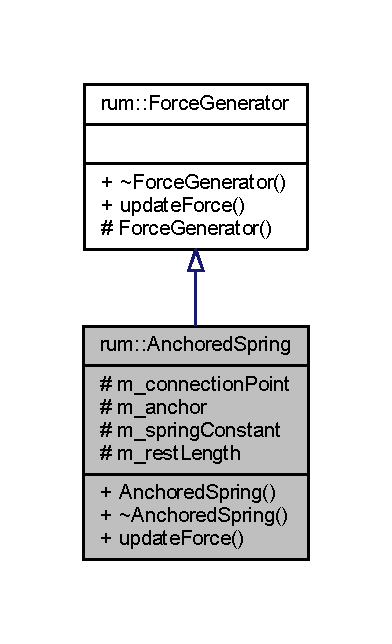
\includegraphics[width=188pt]{classrum_1_1_anchored_spring__inherit__graph}
\end{center}
\end{figure}


Collaboration diagram for rum\+:\+:Anchored\+Spring\+:\nopagebreak
\begin{figure}[H]
\begin{center}
\leavevmode
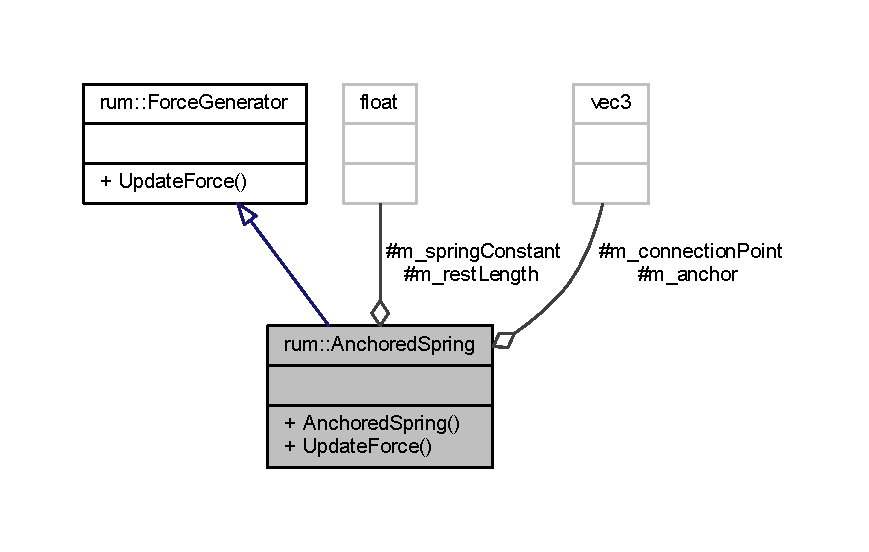
\includegraphics[width=350pt]{classrum_1_1_anchored_spring__coll__graph}
\end{center}
\end{figure}
\subsection*{Public Member Functions}
\begin{DoxyCompactItemize}
\item 
\mbox{\hyperlink{classrum_1_1_anchored_spring_a3bce11c4c0009f1ae3da23525cb99d6c}{Anchored\+Spring}} (const glm\+::vec3 \&anchor, const glm\+::vec3 \&local\+Connection\+Point, \mbox{\hyperlink{namespacerum_a7e8cca23573d5eaead0f138cbaa4862c}{real}} spring\+Constant, \mbox{\hyperlink{namespacerum_a7e8cca23573d5eaead0f138cbaa4862c}{real}} rest\+Length)
\item 
\mbox{\hyperlink{classrum_1_1_anchored_spring_a674ab5042f8a16e50f6635b2b7737b86}{$\sim$\+Anchored\+Spring}} ()
\item 
void \mbox{\hyperlink{classrum_1_1_anchored_spring_aeb146ac725ea6f9ee9c52b322ba70452}{update\+Force}} (\mbox{\hyperlink{classrum_1_1_rigid_body}{Rigid\+Body}} $\ast$body, \mbox{\hyperlink{namespacerum_a7e8cca23573d5eaead0f138cbaa4862c}{real}} duration) override
\end{DoxyCompactItemize}
\subsection*{Protected Attributes}
\begin{DoxyCompactItemize}
\item 
glm\+::vec3 \mbox{\hyperlink{classrum_1_1_anchored_spring_ab828f6a46832b1a36909bf858608579b}{m\+\_\+connection\+Point}}
\item 
glm\+::vec3 \mbox{\hyperlink{classrum_1_1_anchored_spring_ae13ff4ceb813a9e88182fdf04d890d08}{m\+\_\+anchor}}
\item 
\mbox{\hyperlink{namespacerum_a7e8cca23573d5eaead0f138cbaa4862c}{real}} \mbox{\hyperlink{classrum_1_1_anchored_spring_a9ceccbbc91b17c65825827b595d242d2}{m\+\_\+spring\+Constant}}
\item 
\mbox{\hyperlink{namespacerum_a7e8cca23573d5eaead0f138cbaa4862c}{real}} \mbox{\hyperlink{classrum_1_1_anchored_spring_a399861e72ff803834a5203f79741653c}{m\+\_\+rest\+Length}}
\end{DoxyCompactItemize}
\subsection*{Additional Inherited Members}


\subsection{Constructor \& Destructor Documentation}
\mbox{\Hypertarget{classrum_1_1_anchored_spring_a3bce11c4c0009f1ae3da23525cb99d6c}\label{classrum_1_1_anchored_spring_a3bce11c4c0009f1ae3da23525cb99d6c}} 
\index{rum\+::\+Anchored\+Spring@{rum\+::\+Anchored\+Spring}!Anchored\+Spring@{Anchored\+Spring}}
\index{Anchored\+Spring@{Anchored\+Spring}!rum\+::\+Anchored\+Spring@{rum\+::\+Anchored\+Spring}}
\subsubsection{\texorpdfstring{Anchored\+Spring()}{AnchoredSpring()}}
{\footnotesize\ttfamily rum\+::\+Anchored\+Spring\+::\+Anchored\+Spring (\begin{DoxyParamCaption}\item[{const glm\+::vec3 \&}]{anchor,  }\item[{const glm\+::vec3 \&}]{local\+Connection\+Point,  }\item[{\mbox{\hyperlink{namespacerum_a7e8cca23573d5eaead0f138cbaa4862c}{real}}}]{spring\+Constant,  }\item[{\mbox{\hyperlink{namespacerum_a7e8cca23573d5eaead0f138cbaa4862c}{real}}}]{rest\+Length }\end{DoxyParamCaption})\hspace{0.3cm}{\ttfamily [explicit]}}

\mbox{\Hypertarget{classrum_1_1_anchored_spring_a674ab5042f8a16e50f6635b2b7737b86}\label{classrum_1_1_anchored_spring_a674ab5042f8a16e50f6635b2b7737b86}} 
\index{rum\+::\+Anchored\+Spring@{rum\+::\+Anchored\+Spring}!````~Anchored\+Spring@{$\sim$\+Anchored\+Spring}}
\index{````~Anchored\+Spring@{$\sim$\+Anchored\+Spring}!rum\+::\+Anchored\+Spring@{rum\+::\+Anchored\+Spring}}
\subsubsection{\texorpdfstring{$\sim$\+Anchored\+Spring()}{~AnchoredSpring()}}
{\footnotesize\ttfamily rum\+::\+Anchored\+Spring\+::$\sim$\+Anchored\+Spring (\begin{DoxyParamCaption}{ }\end{DoxyParamCaption})\hspace{0.3cm}{\ttfamily [default]}}



\subsection{Member Function Documentation}
\mbox{\Hypertarget{classrum_1_1_anchored_spring_aeb146ac725ea6f9ee9c52b322ba70452}\label{classrum_1_1_anchored_spring_aeb146ac725ea6f9ee9c52b322ba70452}} 
\index{rum\+::\+Anchored\+Spring@{rum\+::\+Anchored\+Spring}!update\+Force@{update\+Force}}
\index{update\+Force@{update\+Force}!rum\+::\+Anchored\+Spring@{rum\+::\+Anchored\+Spring}}
\subsubsection{\texorpdfstring{update\+Force()}{updateForce()}}
{\footnotesize\ttfamily void rum\+::\+Anchored\+Spring\+::update\+Force (\begin{DoxyParamCaption}\item[{\mbox{\hyperlink{classrum_1_1_rigid_body}{Rigid\+Body}} $\ast$}]{body,  }\item[{\mbox{\hyperlink{namespacerum_a7e8cca23573d5eaead0f138cbaa4862c}{real}}}]{duration }\end{DoxyParamCaption})\hspace{0.3cm}{\ttfamily [override]}, {\ttfamily [virtual]}}



Reimplemented from \mbox{\hyperlink{classrum_1_1_force_generator_aee5f1dc03ba285b5122fa2a8ba790230}{rum\+::\+Force\+Generator}}.



\subsection{Member Data Documentation}
\mbox{\Hypertarget{classrum_1_1_anchored_spring_ae13ff4ceb813a9e88182fdf04d890d08}\label{classrum_1_1_anchored_spring_ae13ff4ceb813a9e88182fdf04d890d08}} 
\index{rum\+::\+Anchored\+Spring@{rum\+::\+Anchored\+Spring}!m\+\_\+anchor@{m\+\_\+anchor}}
\index{m\+\_\+anchor@{m\+\_\+anchor}!rum\+::\+Anchored\+Spring@{rum\+::\+Anchored\+Spring}}
\subsubsection{\texorpdfstring{m\+\_\+anchor}{m\_anchor}}
{\footnotesize\ttfamily glm\+::vec3 rum\+::\+Anchored\+Spring\+::m\+\_\+anchor\hspace{0.3cm}{\ttfamily [protected]}}

\mbox{\Hypertarget{classrum_1_1_anchored_spring_ab828f6a46832b1a36909bf858608579b}\label{classrum_1_1_anchored_spring_ab828f6a46832b1a36909bf858608579b}} 
\index{rum\+::\+Anchored\+Spring@{rum\+::\+Anchored\+Spring}!m\+\_\+connection\+Point@{m\+\_\+connection\+Point}}
\index{m\+\_\+connection\+Point@{m\+\_\+connection\+Point}!rum\+::\+Anchored\+Spring@{rum\+::\+Anchored\+Spring}}
\subsubsection{\texorpdfstring{m\+\_\+connection\+Point}{m\_connectionPoint}}
{\footnotesize\ttfamily glm\+::vec3 rum\+::\+Anchored\+Spring\+::m\+\_\+connection\+Point\hspace{0.3cm}{\ttfamily [protected]}}

\mbox{\Hypertarget{classrum_1_1_anchored_spring_a399861e72ff803834a5203f79741653c}\label{classrum_1_1_anchored_spring_a399861e72ff803834a5203f79741653c}} 
\index{rum\+::\+Anchored\+Spring@{rum\+::\+Anchored\+Spring}!m\+\_\+rest\+Length@{m\+\_\+rest\+Length}}
\index{m\+\_\+rest\+Length@{m\+\_\+rest\+Length}!rum\+::\+Anchored\+Spring@{rum\+::\+Anchored\+Spring}}
\subsubsection{\texorpdfstring{m\+\_\+rest\+Length}{m\_restLength}}
{\footnotesize\ttfamily \mbox{\hyperlink{namespacerum_a7e8cca23573d5eaead0f138cbaa4862c}{real}} rum\+::\+Anchored\+Spring\+::m\+\_\+rest\+Length\hspace{0.3cm}{\ttfamily [protected]}}

\mbox{\Hypertarget{classrum_1_1_anchored_spring_a9ceccbbc91b17c65825827b595d242d2}\label{classrum_1_1_anchored_spring_a9ceccbbc91b17c65825827b595d242d2}} 
\index{rum\+::\+Anchored\+Spring@{rum\+::\+Anchored\+Spring}!m\+\_\+spring\+Constant@{m\+\_\+spring\+Constant}}
\index{m\+\_\+spring\+Constant@{m\+\_\+spring\+Constant}!rum\+::\+Anchored\+Spring@{rum\+::\+Anchored\+Spring}}
\subsubsection{\texorpdfstring{m\+\_\+spring\+Constant}{m\_springConstant}}
{\footnotesize\ttfamily \mbox{\hyperlink{namespacerum_a7e8cca23573d5eaead0f138cbaa4862c}{real}} rum\+::\+Anchored\+Spring\+::m\+\_\+spring\+Constant\hspace{0.3cm}{\ttfamily [protected]}}



The documentation for this class was generated from the following files\+:\begin{DoxyCompactItemize}
\item 
D\+:/\+Library/\+Documents/\+Job/\+Forschungsmaster/\+Projekte/\+Rumble3\+D/\+Rumble3\+D/include/\+R3\+D/\+Rigid\+Body\+Engine/\mbox{\hyperlink{_anchored_spring_8h}{Anchored\+Spring.\+h}}\item 
D\+:/\+Library/\+Documents/\+Job/\+Forschungsmaster/\+Projekte/\+Rumble3\+D/\+Rumble3\+D/src/\+Rigid\+Body\+Engine/\mbox{\hyperlink{_anchored_spring_8cpp}{Anchored\+Spring.\+cpp}}\end{DoxyCompactItemize}

\hypertarget{classrum_1_1_bounding_box}{}\section{rum\+:\+:Bounding\+Box Class Reference}
\label{classrum_1_1_bounding_box}\index{rum\+::\+Bounding\+Box@{rum\+::\+Bounding\+Box}}


{\ttfamily \#include $<$Bounding\+Box.\+h$>$}



Collaboration diagram for rum\+:\+:Bounding\+Box\+:\nopagebreak
\begin{figure}[H]
\begin{center}
\leavevmode
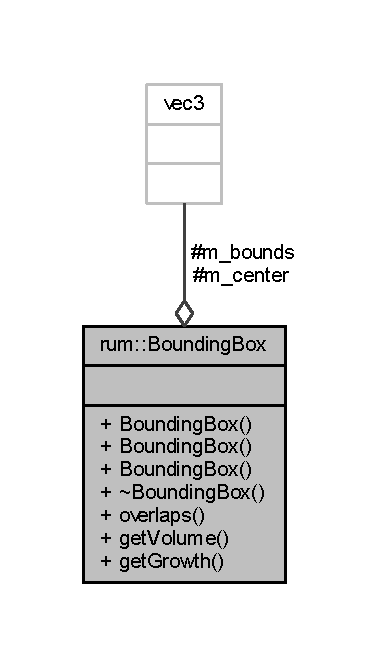
\includegraphics[width=183pt]{classrum_1_1_bounding_box__coll__graph}
\end{center}
\end{figure}
\subsection*{Public Member Functions}
\begin{DoxyCompactItemize}
\item 
\hyperlink{classrum_1_1_bounding_box_ab8fc622a27065c0bfe9e9f3d057c900e}{Bounding\+Box} ()
\item 
\hyperlink{classrum_1_1_bounding_box_a60123b8bafc7fa4ef78cdf2a4c49eac3}{Bounding\+Box} (const glm\+::vec3 \&center, const glm\+::vec3 \&bounds)
\item 
\hyperlink{classrum_1_1_bounding_box_a68f722c0cc72e5c939fa1fa382b26330}{Bounding\+Box} (const \hyperlink{classrum_1_1_bounding_box}{Bounding\+Box} \&one, const \hyperlink{classrum_1_1_bounding_box}{Bounding\+Box} \&two)
\item 
\hyperlink{classrum_1_1_bounding_box_a515a617dd779ad1932598f0bb6bd9669}{$\sim$\+Bounding\+Box} ()
\item 
bool \hyperlink{classrum_1_1_bounding_box_af7d2034adecd49f949b7bf5bfa942498}{Overlaps} (const \hyperlink{classrum_1_1_bounding_box}{Bounding\+Box} $\ast$other) const
\item 
\hyperlink{namespacerum_a7e8cca23573d5eaead0f138cbaa4862c}{real} \hyperlink{classrum_1_1_bounding_box_add513abe94c5ad77ff3ec2f29b6d6241}{Get\+Size} () const
\item 
\hyperlink{namespacerum_a7e8cca23573d5eaead0f138cbaa4862c}{real} \hyperlink{classrum_1_1_bounding_box_a944672fb8a07383cf4409393a62ffc1f}{Get\+Growth} (const \hyperlink{classrum_1_1_bounding_box}{Bounding\+Box} \&other) const
\end{DoxyCompactItemize}
\subsection*{Protected Attributes}
\begin{DoxyCompactItemize}
\item 
glm\+::vec3 \hyperlink{classrum_1_1_bounding_box_af9c7a5df5b02f646a1aa0d5cf0c4e1fd}{m\+\_\+center}
\item 
glm\+::vec3 \hyperlink{classrum_1_1_bounding_box_a676df9315a0bf21962b02c65cb765a3a}{m\+\_\+bounds}
\end{DoxyCompactItemize}


\subsection{Constructor \& Destructor Documentation}
\mbox{\Hypertarget{classrum_1_1_bounding_box_ab8fc622a27065c0bfe9e9f3d057c900e}\label{classrum_1_1_bounding_box_ab8fc622a27065c0bfe9e9f3d057c900e}} 
\index{rum\+::\+Bounding\+Box@{rum\+::\+Bounding\+Box}!Bounding\+Box@{Bounding\+Box}}
\index{Bounding\+Box@{Bounding\+Box}!rum\+::\+Bounding\+Box@{rum\+::\+Bounding\+Box}}
\subsubsection{\texorpdfstring{Bounding\+Box()}{BoundingBox()}\hspace{0.1cm}{\footnotesize\ttfamily [1/3]}}
{\footnotesize\ttfamily rum\+::\+Bounding\+Box\+::\+Bounding\+Box (\begin{DoxyParamCaption}{ }\end{DoxyParamCaption})}

\mbox{\Hypertarget{classrum_1_1_bounding_box_a60123b8bafc7fa4ef78cdf2a4c49eac3}\label{classrum_1_1_bounding_box_a60123b8bafc7fa4ef78cdf2a4c49eac3}} 
\index{rum\+::\+Bounding\+Box@{rum\+::\+Bounding\+Box}!Bounding\+Box@{Bounding\+Box}}
\index{Bounding\+Box@{Bounding\+Box}!rum\+::\+Bounding\+Box@{rum\+::\+Bounding\+Box}}
\subsubsection{\texorpdfstring{Bounding\+Box()}{BoundingBox()}\hspace{0.1cm}{\footnotesize\ttfamily [2/3]}}
{\footnotesize\ttfamily rum\+::\+Bounding\+Box\+::\+Bounding\+Box (\begin{DoxyParamCaption}\item[{const glm\+::vec3 \&}]{center,  }\item[{const glm\+::vec3 \&}]{bounds }\end{DoxyParamCaption})}

\mbox{\Hypertarget{classrum_1_1_bounding_box_a68f722c0cc72e5c939fa1fa382b26330}\label{classrum_1_1_bounding_box_a68f722c0cc72e5c939fa1fa382b26330}} 
\index{rum\+::\+Bounding\+Box@{rum\+::\+Bounding\+Box}!Bounding\+Box@{Bounding\+Box}}
\index{Bounding\+Box@{Bounding\+Box}!rum\+::\+Bounding\+Box@{rum\+::\+Bounding\+Box}}
\subsubsection{\texorpdfstring{Bounding\+Box()}{BoundingBox()}\hspace{0.1cm}{\footnotesize\ttfamily [3/3]}}
{\footnotesize\ttfamily rum\+::\+Bounding\+Box\+::\+Bounding\+Box (\begin{DoxyParamCaption}\item[{const \hyperlink{classrum_1_1_bounding_box}{Bounding\+Box} \&}]{one,  }\item[{const \hyperlink{classrum_1_1_bounding_box}{Bounding\+Box} \&}]{two }\end{DoxyParamCaption})}

\mbox{\Hypertarget{classrum_1_1_bounding_box_a515a617dd779ad1932598f0bb6bd9669}\label{classrum_1_1_bounding_box_a515a617dd779ad1932598f0bb6bd9669}} 
\index{rum\+::\+Bounding\+Box@{rum\+::\+Bounding\+Box}!````~Bounding\+Box@{$\sim$\+Bounding\+Box}}
\index{````~Bounding\+Box@{$\sim$\+Bounding\+Box}!rum\+::\+Bounding\+Box@{rum\+::\+Bounding\+Box}}
\subsubsection{\texorpdfstring{$\sim$\+Bounding\+Box()}{~BoundingBox()}}
{\footnotesize\ttfamily rum\+::\+Bounding\+Box\+::$\sim$\+Bounding\+Box (\begin{DoxyParamCaption}{ }\end{DoxyParamCaption})}



\subsection{Member Function Documentation}
\mbox{\Hypertarget{classrum_1_1_bounding_box_a944672fb8a07383cf4409393a62ffc1f}\label{classrum_1_1_bounding_box_a944672fb8a07383cf4409393a62ffc1f}} 
\index{rum\+::\+Bounding\+Box@{rum\+::\+Bounding\+Box}!Get\+Growth@{Get\+Growth}}
\index{Get\+Growth@{Get\+Growth}!rum\+::\+Bounding\+Box@{rum\+::\+Bounding\+Box}}
\subsubsection{\texorpdfstring{Get\+Growth()}{GetGrowth()}}
{\footnotesize\ttfamily \hyperlink{namespacerum_a7e8cca23573d5eaead0f138cbaa4862c}{real} rum\+::\+Bounding\+Box\+::\+Get\+Growth (\begin{DoxyParamCaption}\item[{const \hyperlink{classrum_1_1_bounding_box}{Bounding\+Box} \&}]{other }\end{DoxyParamCaption}) const}

\mbox{\Hypertarget{classrum_1_1_bounding_box_add513abe94c5ad77ff3ec2f29b6d6241}\label{classrum_1_1_bounding_box_add513abe94c5ad77ff3ec2f29b6d6241}} 
\index{rum\+::\+Bounding\+Box@{rum\+::\+Bounding\+Box}!Get\+Size@{Get\+Size}}
\index{Get\+Size@{Get\+Size}!rum\+::\+Bounding\+Box@{rum\+::\+Bounding\+Box}}
\subsubsection{\texorpdfstring{Get\+Size()}{GetSize()}}
{\footnotesize\ttfamily \hyperlink{namespacerum_a7e8cca23573d5eaead0f138cbaa4862c}{real} rum\+::\+Bounding\+Box\+::\+Get\+Size (\begin{DoxyParamCaption}{ }\end{DoxyParamCaption}) const}

\mbox{\Hypertarget{classrum_1_1_bounding_box_af7d2034adecd49f949b7bf5bfa942498}\label{classrum_1_1_bounding_box_af7d2034adecd49f949b7bf5bfa942498}} 
\index{rum\+::\+Bounding\+Box@{rum\+::\+Bounding\+Box}!Overlaps@{Overlaps}}
\index{Overlaps@{Overlaps}!rum\+::\+Bounding\+Box@{rum\+::\+Bounding\+Box}}
\subsubsection{\texorpdfstring{Overlaps()}{Overlaps()}}
{\footnotesize\ttfamily bool rum\+::\+Bounding\+Box\+::\+Overlaps (\begin{DoxyParamCaption}\item[{const \hyperlink{classrum_1_1_bounding_box}{Bounding\+Box} $\ast$}]{other }\end{DoxyParamCaption}) const}



\subsection{Member Data Documentation}
\mbox{\Hypertarget{classrum_1_1_bounding_box_a676df9315a0bf21962b02c65cb765a3a}\label{classrum_1_1_bounding_box_a676df9315a0bf21962b02c65cb765a3a}} 
\index{rum\+::\+Bounding\+Box@{rum\+::\+Bounding\+Box}!m\+\_\+bounds@{m\+\_\+bounds}}
\index{m\+\_\+bounds@{m\+\_\+bounds}!rum\+::\+Bounding\+Box@{rum\+::\+Bounding\+Box}}
\subsubsection{\texorpdfstring{m\+\_\+bounds}{m\_bounds}}
{\footnotesize\ttfamily glm\+::vec3 rum\+::\+Bounding\+Box\+::m\+\_\+bounds\hspace{0.3cm}{\ttfamily [protected]}}

\mbox{\Hypertarget{classrum_1_1_bounding_box_af9c7a5df5b02f646a1aa0d5cf0c4e1fd}\label{classrum_1_1_bounding_box_af9c7a5df5b02f646a1aa0d5cf0c4e1fd}} 
\index{rum\+::\+Bounding\+Box@{rum\+::\+Bounding\+Box}!m\+\_\+center@{m\+\_\+center}}
\index{m\+\_\+center@{m\+\_\+center}!rum\+::\+Bounding\+Box@{rum\+::\+Bounding\+Box}}
\subsubsection{\texorpdfstring{m\+\_\+center}{m\_center}}
{\footnotesize\ttfamily glm\+::vec3 rum\+::\+Bounding\+Box\+::m\+\_\+center\hspace{0.3cm}{\ttfamily [protected]}}



The documentation for this class was generated from the following files\+:\begin{DoxyCompactItemize}
\item 
F\+:/\+Library/\+Documents/\+Job/\+Forschungsmaster/\+Rumble3\+D/\+Rumble3\+D/include/\+R3\+D/\+Rigid\+Body\+Engine/\hyperlink{_bounding_box_8h}{Bounding\+Box.\+h}\item 
F\+:/\+Library/\+Documents/\+Job/\+Forschungsmaster/\+Rumble3\+D/\+Rumble3\+D/src/\+Rigid\+Body\+Engine/\hyperlink{_bounding_box_8cpp}{Bounding\+Box.\+cpp}\end{DoxyCompactItemize}

\hypertarget{classrum_1_1_bounding_sphere}{}\section{rum\+:\+:Bounding\+Sphere Class Reference}
\label{classrum_1_1_bounding_sphere}\index{rum\+::\+Bounding\+Sphere@{rum\+::\+Bounding\+Sphere}}


{\ttfamily \#include $<$Bounding\+Sphere.\+h$>$}



Collaboration diagram for rum\+:\+:Bounding\+Sphere\+:\nopagebreak
\begin{figure}[H]
\begin{center}
\leavevmode
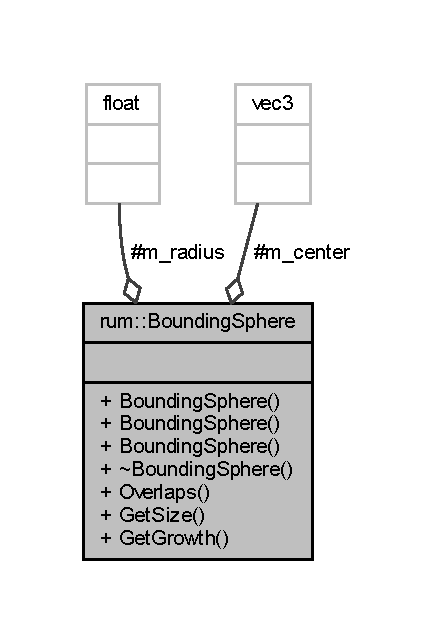
\includegraphics[width=208pt]{classrum_1_1_bounding_sphere__coll__graph}
\end{center}
\end{figure}
\subsection*{Public Member Functions}
\begin{DoxyCompactItemize}
\item 
\mbox{\hyperlink{classrum_1_1_bounding_sphere_a9fcd71c636d8603a7f2b8bf0571187ef}{Bounding\+Sphere}} ()
\item 
\mbox{\hyperlink{classrum_1_1_bounding_sphere_adc0112926da70e6670fd75feb04ba1d0}{Bounding\+Sphere}} (const glm\+::vec3 \&center, \mbox{\hyperlink{namespacerum_a7e8cca23573d5eaead0f138cbaa4862c}{real}} radius)
\item 
\mbox{\hyperlink{classrum_1_1_bounding_sphere_ad97a79a4d245770556b3526d3db9cad8}{Bounding\+Sphere}} (const \mbox{\hyperlink{classrum_1_1_bounding_sphere}{Bounding\+Sphere}} \&one, const \mbox{\hyperlink{classrum_1_1_bounding_sphere}{Bounding\+Sphere}} \&two)
\item 
\mbox{\hyperlink{classrum_1_1_bounding_sphere_a2a6e3e469ebaa4a783cc0688c065d171}{$\sim$\+Bounding\+Sphere}} ()
\item 
bool \mbox{\hyperlink{classrum_1_1_bounding_sphere_a14ef0d9e7cfd2f85b98e1ddb9c8b6b78}{overlaps}} (const \mbox{\hyperlink{classrum_1_1_bounding_sphere}{Bounding\+Sphere}} $\ast$other) const
\item 
\mbox{\hyperlink{namespacerum_a7e8cca23573d5eaead0f138cbaa4862c}{real}} \mbox{\hyperlink{classrum_1_1_bounding_sphere_a08f598ea27ab22c1eb18db9fcc2fa4da}{get\+Volume}} () const
\item 
\mbox{\hyperlink{namespacerum_a7e8cca23573d5eaead0f138cbaa4862c}{real}} \mbox{\hyperlink{classrum_1_1_bounding_sphere_abde38ee4e771f41c6128a42856ac5514}{get\+Growth}} (const \mbox{\hyperlink{classrum_1_1_bounding_sphere}{Bounding\+Sphere}} \&other) const
\end{DoxyCompactItemize}
\subsection*{Protected Attributes}
\begin{DoxyCompactItemize}
\item 
glm\+::vec3 \mbox{\hyperlink{classrum_1_1_bounding_sphere_acc7a118371f95f36831b12c1862fbfb1}{m\+\_\+center}}
\item 
\mbox{\hyperlink{namespacerum_a7e8cca23573d5eaead0f138cbaa4862c}{real}} \mbox{\hyperlink{classrum_1_1_bounding_sphere_acc810ba77f514caeef45a248f2ffb67c}{m\+\_\+radius}} \{\}
\end{DoxyCompactItemize}


\subsection{Constructor \& Destructor Documentation}
\mbox{\Hypertarget{classrum_1_1_bounding_sphere_a9fcd71c636d8603a7f2b8bf0571187ef}\label{classrum_1_1_bounding_sphere_a9fcd71c636d8603a7f2b8bf0571187ef}} 
\index{rum\+::\+Bounding\+Sphere@{rum\+::\+Bounding\+Sphere}!Bounding\+Sphere@{Bounding\+Sphere}}
\index{Bounding\+Sphere@{Bounding\+Sphere}!rum\+::\+Bounding\+Sphere@{rum\+::\+Bounding\+Sphere}}
\subsubsection{\texorpdfstring{Bounding\+Sphere()}{BoundingSphere()}\hspace{0.1cm}{\footnotesize\ttfamily [1/3]}}
{\footnotesize\ttfamily rum\+::\+Bounding\+Sphere\+::\+Bounding\+Sphere (\begin{DoxyParamCaption}{ }\end{DoxyParamCaption})\hspace{0.3cm}{\ttfamily [default]}}

\mbox{\Hypertarget{classrum_1_1_bounding_sphere_adc0112926da70e6670fd75feb04ba1d0}\label{classrum_1_1_bounding_sphere_adc0112926da70e6670fd75feb04ba1d0}} 
\index{rum\+::\+Bounding\+Sphere@{rum\+::\+Bounding\+Sphere}!Bounding\+Sphere@{Bounding\+Sphere}}
\index{Bounding\+Sphere@{Bounding\+Sphere}!rum\+::\+Bounding\+Sphere@{rum\+::\+Bounding\+Sphere}}
\subsubsection{\texorpdfstring{Bounding\+Sphere()}{BoundingSphere()}\hspace{0.1cm}{\footnotesize\ttfamily [2/3]}}
{\footnotesize\ttfamily rum\+::\+Bounding\+Sphere\+::\+Bounding\+Sphere (\begin{DoxyParamCaption}\item[{const glm\+::vec3 \&}]{center,  }\item[{\mbox{\hyperlink{namespacerum_a7e8cca23573d5eaead0f138cbaa4862c}{real}}}]{radius }\end{DoxyParamCaption})}

\mbox{\Hypertarget{classrum_1_1_bounding_sphere_ad97a79a4d245770556b3526d3db9cad8}\label{classrum_1_1_bounding_sphere_ad97a79a4d245770556b3526d3db9cad8}} 
\index{rum\+::\+Bounding\+Sphere@{rum\+::\+Bounding\+Sphere}!Bounding\+Sphere@{Bounding\+Sphere}}
\index{Bounding\+Sphere@{Bounding\+Sphere}!rum\+::\+Bounding\+Sphere@{rum\+::\+Bounding\+Sphere}}
\subsubsection{\texorpdfstring{Bounding\+Sphere()}{BoundingSphere()}\hspace{0.1cm}{\footnotesize\ttfamily [3/3]}}
{\footnotesize\ttfamily rum\+::\+Bounding\+Sphere\+::\+Bounding\+Sphere (\begin{DoxyParamCaption}\item[{const \mbox{\hyperlink{classrum_1_1_bounding_sphere}{Bounding\+Sphere}} \&}]{one,  }\item[{const \mbox{\hyperlink{classrum_1_1_bounding_sphere}{Bounding\+Sphere}} \&}]{two }\end{DoxyParamCaption})}

Create a bounding sphere which contains both given spheres. \mbox{\Hypertarget{classrum_1_1_bounding_sphere_a2a6e3e469ebaa4a783cc0688c065d171}\label{classrum_1_1_bounding_sphere_a2a6e3e469ebaa4a783cc0688c065d171}} 
\index{rum\+::\+Bounding\+Sphere@{rum\+::\+Bounding\+Sphere}!````~Bounding\+Sphere@{$\sim$\+Bounding\+Sphere}}
\index{````~Bounding\+Sphere@{$\sim$\+Bounding\+Sphere}!rum\+::\+Bounding\+Sphere@{rum\+::\+Bounding\+Sphere}}
\subsubsection{\texorpdfstring{$\sim$\+Bounding\+Sphere()}{~BoundingSphere()}}
{\footnotesize\ttfamily rum\+::\+Bounding\+Sphere\+::$\sim$\+Bounding\+Sphere (\begin{DoxyParamCaption}{ }\end{DoxyParamCaption})\hspace{0.3cm}{\ttfamily [default]}}



\subsection{Member Function Documentation}
\mbox{\Hypertarget{classrum_1_1_bounding_sphere_abde38ee4e771f41c6128a42856ac5514}\label{classrum_1_1_bounding_sphere_abde38ee4e771f41c6128a42856ac5514}} 
\index{rum\+::\+Bounding\+Sphere@{rum\+::\+Bounding\+Sphere}!get\+Growth@{get\+Growth}}
\index{get\+Growth@{get\+Growth}!rum\+::\+Bounding\+Sphere@{rum\+::\+Bounding\+Sphere}}
\subsubsection{\texorpdfstring{get\+Growth()}{getGrowth()}}
{\footnotesize\ttfamily \mbox{\hyperlink{namespacerum_a7e8cca23573d5eaead0f138cbaa4862c}{real}} rum\+::\+Bounding\+Sphere\+::get\+Growth (\begin{DoxyParamCaption}\item[{const \mbox{\hyperlink{classrum_1_1_bounding_sphere}{Bounding\+Sphere}} \&}]{other }\end{DoxyParamCaption}) const}

Gibt einen Wert zur�ck, der das Wachstum einer Kugel durch eine andere Kugel beschreibt, indem N�herungen der Oberfl�chen berechnet werden. \mbox{\Hypertarget{classrum_1_1_bounding_sphere_a08f598ea27ab22c1eb18db9fcc2fa4da}\label{classrum_1_1_bounding_sphere_a08f598ea27ab22c1eb18db9fcc2fa4da}} 
\index{rum\+::\+Bounding\+Sphere@{rum\+::\+Bounding\+Sphere}!get\+Volume@{get\+Volume}}
\index{get\+Volume@{get\+Volume}!rum\+::\+Bounding\+Sphere@{rum\+::\+Bounding\+Sphere}}
\subsubsection{\texorpdfstring{get\+Volume()}{getVolume()}}
{\footnotesize\ttfamily \mbox{\hyperlink{namespacerum_a7e8cca23573d5eaead0f138cbaa4862c}{real}} rum\+::\+Bounding\+Sphere\+::get\+Volume (\begin{DoxyParamCaption}{ }\end{DoxyParamCaption}) const}

Get the volume of this bounding sphere. \mbox{\Hypertarget{classrum_1_1_bounding_sphere_a14ef0d9e7cfd2f85b98e1ddb9c8b6b78}\label{classrum_1_1_bounding_sphere_a14ef0d9e7cfd2f85b98e1ddb9c8b6b78}} 
\index{rum\+::\+Bounding\+Sphere@{rum\+::\+Bounding\+Sphere}!overlaps@{overlaps}}
\index{overlaps@{overlaps}!rum\+::\+Bounding\+Sphere@{rum\+::\+Bounding\+Sphere}}
\subsubsection{\texorpdfstring{overlaps()}{overlaps()}}
{\footnotesize\ttfamily bool rum\+::\+Bounding\+Sphere\+::overlaps (\begin{DoxyParamCaption}\item[{const \mbox{\hyperlink{classrum_1_1_bounding_sphere}{Bounding\+Sphere}} $\ast$}]{other }\end{DoxyParamCaption}) const}

Check if this bounding sphere overlaps with the given bounding sphere \begin{DoxyReturn}{Returns}
True if they overlap, false otherwise. 
\end{DoxyReturn}


\subsection{Member Data Documentation}
\mbox{\Hypertarget{classrum_1_1_bounding_sphere_acc7a118371f95f36831b12c1862fbfb1}\label{classrum_1_1_bounding_sphere_acc7a118371f95f36831b12c1862fbfb1}} 
\index{rum\+::\+Bounding\+Sphere@{rum\+::\+Bounding\+Sphere}!m\+\_\+center@{m\+\_\+center}}
\index{m\+\_\+center@{m\+\_\+center}!rum\+::\+Bounding\+Sphere@{rum\+::\+Bounding\+Sphere}}
\subsubsection{\texorpdfstring{m\+\_\+center}{m\_center}}
{\footnotesize\ttfamily glm\+::vec3 rum\+::\+Bounding\+Sphere\+::m\+\_\+center\hspace{0.3cm}{\ttfamily [protected]}}

\mbox{\Hypertarget{classrum_1_1_bounding_sphere_acc810ba77f514caeef45a248f2ffb67c}\label{classrum_1_1_bounding_sphere_acc810ba77f514caeef45a248f2ffb67c}} 
\index{rum\+::\+Bounding\+Sphere@{rum\+::\+Bounding\+Sphere}!m\+\_\+radius@{m\+\_\+radius}}
\index{m\+\_\+radius@{m\+\_\+radius}!rum\+::\+Bounding\+Sphere@{rum\+::\+Bounding\+Sphere}}
\subsubsection{\texorpdfstring{m\+\_\+radius}{m\_radius}}
{\footnotesize\ttfamily \mbox{\hyperlink{namespacerum_a7e8cca23573d5eaead0f138cbaa4862c}{real}} rum\+::\+Bounding\+Sphere\+::m\+\_\+radius \{\}\hspace{0.3cm}{\ttfamily [protected]}}



The documentation for this class was generated from the following files\+:\begin{DoxyCompactItemize}
\item 
D\+:/\+Library/\+Documents/\+Job/\+Forschungsmaster/\+Projekte/\+Rumble3\+D/\+Rumble3\+D/include/\+R3\+D/\+Rigid\+Body\+Engine/\mbox{\hyperlink{_bounding_sphere_8h}{Bounding\+Sphere.\+h}}\item 
D\+:/\+Library/\+Documents/\+Job/\+Forschungsmaster/\+Projekte/\+Rumble3\+D/\+Rumble3\+D/src/\+Rigid\+Body\+Engine/\mbox{\hyperlink{_bounding_sphere_8cpp}{Bounding\+Sphere.\+cpp}}\end{DoxyCompactItemize}

\hypertarget{classrum_1_1_b_v_h_node}{}\section{rum\+:\+:B\+V\+H\+Node$<$ Bounding\+Volume\+Class $>$ Class Template Reference}
\label{classrum_1_1_b_v_h_node}\index{rum\+::\+B\+V\+H\+Node$<$ Bounding\+Volume\+Class $>$@{rum\+::\+B\+V\+H\+Node$<$ Bounding\+Volume\+Class $>$}}


{\ttfamily \#include $<$B\+V\+H\+Node.\+h$>$}



Collaboration diagram for rum\+:\+:B\+V\+H\+Node$<$ Bounding\+Volume\+Class $>$\+:\nopagebreak
\begin{figure}[H]
\begin{center}
\leavevmode
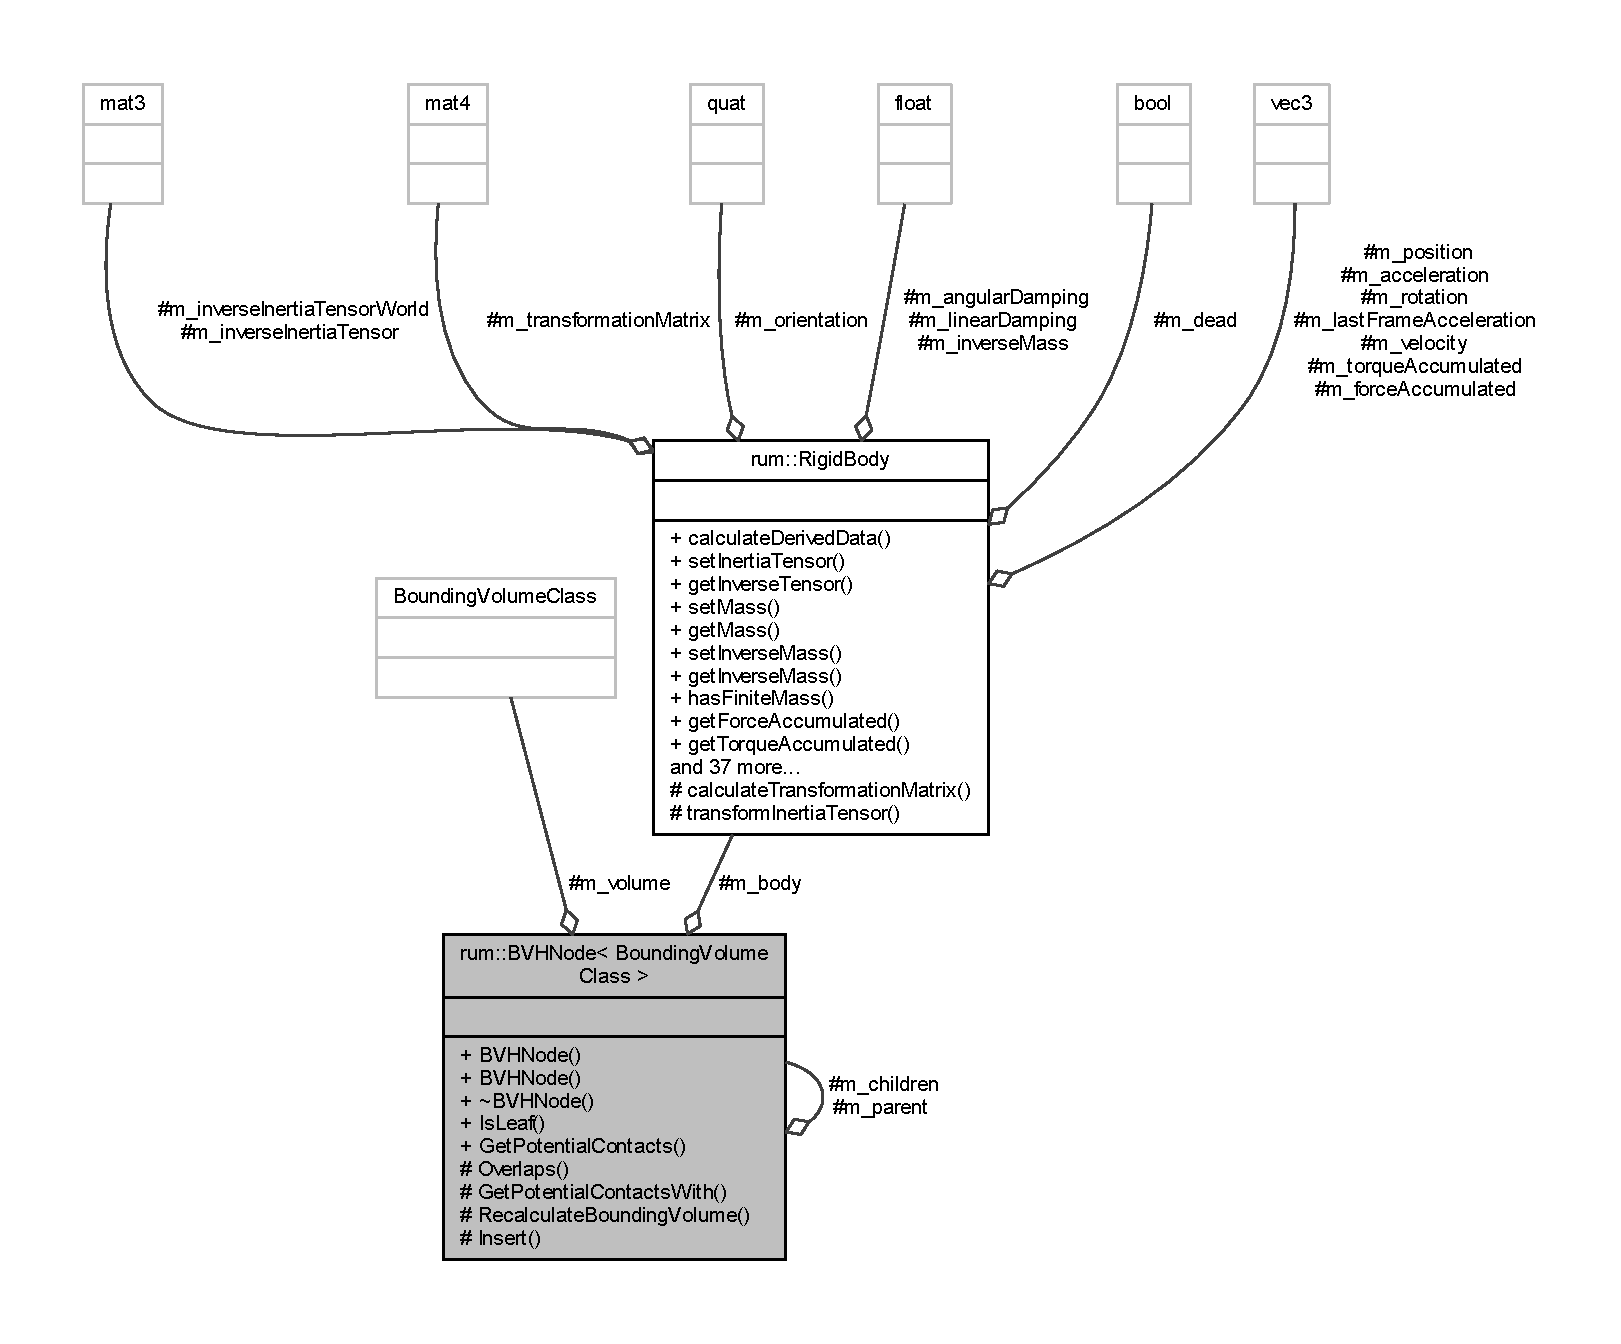
\includegraphics[width=350pt]{classrum_1_1_b_v_h_node__coll__graph}
\end{center}
\end{figure}
\subsection*{Public Member Functions}
\begin{DoxyCompactItemize}
\item 
\hyperlink{classrum_1_1_b_v_h_node_aca2a55118d5c021f92b8e0105fa32625}{B\+V\+H\+Node} ()
\item 
\hyperlink{classrum_1_1_b_v_h_node_a4d6bef35007d6473eefe2ce8979e2e2c}{B\+V\+H\+Node} (\hyperlink{classrum_1_1_b_v_h_node}{B\+V\+H\+Node}$<$ Bounding\+Volume\+Class $>$ $\ast$parent, const Bounding\+Volume\+Class \&volume, \hyperlink{classrum_1_1_rigid_body}{Rigid\+Body} $\ast$body=nullptr)
\item 
\hyperlink{classrum_1_1_b_v_h_node_a97283b0dd8f0cf52762da014a94ade0b}{$\sim$\+B\+V\+H\+Node} ()
\item 
bool \hyperlink{classrum_1_1_b_v_h_node_ad916d1d80373a61b95d99d6ae7472007}{Is\+Leaf} () const
\item 
unsigned int \hyperlink{classrum_1_1_b_v_h_node_a951e91e4c58802cb843e5b0a146c4eb1}{Get\+Potential\+Contacts} (\hyperlink{structrum_1_1_potential_contacts}{Potential\+Contacts} $\ast$contacts, unsigned int limit) const
\end{DoxyCompactItemize}
\subsection*{Protected Member Functions}
\begin{DoxyCompactItemize}
\item 
bool \hyperlink{classrum_1_1_b_v_h_node_a4d60cfdfc53028f0a567fe5f5c316848}{Overlaps} (\hyperlink{classrum_1_1_b_v_h_node}{B\+V\+H\+Node}$<$ Bounding\+Volume\+Class $>$ $\ast$other) const
\item 
unsigned \hyperlink{classrum_1_1_b_v_h_node_a51c82ced5651f99e338bd0ce71700ca6}{Get\+Potential\+Contacts\+With} (\hyperlink{classrum_1_1_b_v_h_node}{B\+V\+H\+Node}$<$ Bounding\+Volume\+Class $>$ $\ast$other, \hyperlink{structrum_1_1_potential_contacts}{Potential\+Contacts} $\ast$contacts, unsigned limit) const
\item 
void \hyperlink{classrum_1_1_b_v_h_node_a8cd9eb8eaf308170ae0350a617210096}{Recalculate\+Bounding\+Volume} ()
\item 
void \hyperlink{classrum_1_1_b_v_h_node_ab74f21c80eb2ad8087b9b897fd3dccd4}{Insert} (\hyperlink{classrum_1_1_rigid_body}{Rigid\+Body} $\ast$new\+Body, const Bounding\+Volume\+Class \&new\+Volume)
\end{DoxyCompactItemize}
\subsection*{Protected Attributes}
\begin{DoxyCompactItemize}
\item 
\hyperlink{classrum_1_1_b_v_h_node}{B\+V\+H\+Node} $\ast$ \hyperlink{classrum_1_1_b_v_h_node_a681ca4a3084ba34bd54c546a7ef2a36c}{m\+\_\+children} \mbox{[}2\mbox{]}
\item 
Bounding\+Volume\+Class \hyperlink{classrum_1_1_b_v_h_node_aae21162bff289e2d0d502c9360d0f36c}{m\+\_\+volume}
\item 
\hyperlink{classrum_1_1_rigid_body}{Rigid\+Body} $\ast$ \hyperlink{classrum_1_1_b_v_h_node_a24954eb90f55a8a29c6459706554c9d6}{m\+\_\+body}
\item 
\hyperlink{classrum_1_1_b_v_h_node}{B\+V\+H\+Node} $\ast$ \hyperlink{classrum_1_1_b_v_h_node_ae69483db4fada9afde3a31393243a87d}{m\+\_\+parent}
\end{DoxyCompactItemize}


\subsection{Constructor \& Destructor Documentation}
\mbox{\Hypertarget{classrum_1_1_b_v_h_node_aca2a55118d5c021f92b8e0105fa32625}\label{classrum_1_1_b_v_h_node_aca2a55118d5c021f92b8e0105fa32625}} 
\index{rum\+::\+B\+V\+H\+Node@{rum\+::\+B\+V\+H\+Node}!B\+V\+H\+Node@{B\+V\+H\+Node}}
\index{B\+V\+H\+Node@{B\+V\+H\+Node}!rum\+::\+B\+V\+H\+Node@{rum\+::\+B\+V\+H\+Node}}
\subsubsection{\texorpdfstring{B\+V\+H\+Node()}{BVHNode()}\hspace{0.1cm}{\footnotesize\ttfamily [1/2]}}
{\footnotesize\ttfamily template$<$class Bounding\+Volume\+Class $>$ \\
\hyperlink{classrum_1_1_b_v_h_node}{rum\+::\+B\+V\+H\+Node}$<$ Bounding\+Volume\+Class $>$\+::\hyperlink{classrum_1_1_b_v_h_node}{B\+V\+H\+Node} (\begin{DoxyParamCaption}{ }\end{DoxyParamCaption})}

\mbox{\Hypertarget{classrum_1_1_b_v_h_node_a4d6bef35007d6473eefe2ce8979e2e2c}\label{classrum_1_1_b_v_h_node_a4d6bef35007d6473eefe2ce8979e2e2c}} 
\index{rum\+::\+B\+V\+H\+Node@{rum\+::\+B\+V\+H\+Node}!B\+V\+H\+Node@{B\+V\+H\+Node}}
\index{B\+V\+H\+Node@{B\+V\+H\+Node}!rum\+::\+B\+V\+H\+Node@{rum\+::\+B\+V\+H\+Node}}
\subsubsection{\texorpdfstring{B\+V\+H\+Node()}{BVHNode()}\hspace{0.1cm}{\footnotesize\ttfamily [2/2]}}
{\footnotesize\ttfamily template$<$class Bounding\+Volume\+Class $>$ \\
\hyperlink{classrum_1_1_b_v_h_node}{rum\+::\+B\+V\+H\+Node}$<$ Bounding\+Volume\+Class $>$\+::\hyperlink{classrum_1_1_b_v_h_node}{B\+V\+H\+Node} (\begin{DoxyParamCaption}\item[{\hyperlink{classrum_1_1_b_v_h_node}{B\+V\+H\+Node}$<$ Bounding\+Volume\+Class $>$ $\ast$}]{parent,  }\item[{const Bounding\+Volume\+Class \&}]{volume,  }\item[{\hyperlink{classrum_1_1_rigid_body}{Rigid\+Body} $\ast$}]{body = {\ttfamily nullptr} }\end{DoxyParamCaption})}

\mbox{\Hypertarget{classrum_1_1_b_v_h_node_a97283b0dd8f0cf52762da014a94ade0b}\label{classrum_1_1_b_v_h_node_a97283b0dd8f0cf52762da014a94ade0b}} 
\index{rum\+::\+B\+V\+H\+Node@{rum\+::\+B\+V\+H\+Node}!````~B\+V\+H\+Node@{$\sim$\+B\+V\+H\+Node}}
\index{````~B\+V\+H\+Node@{$\sim$\+B\+V\+H\+Node}!rum\+::\+B\+V\+H\+Node@{rum\+::\+B\+V\+H\+Node}}
\subsubsection{\texorpdfstring{$\sim$\+B\+V\+H\+Node()}{~BVHNode()}}
{\footnotesize\ttfamily template$<$class Bounding\+Volume\+Class $>$ \\
\hyperlink{classrum_1_1_b_v_h_node}{rum\+::\+B\+V\+H\+Node}$<$ Bounding\+Volume\+Class $>$\+::$\sim$\hyperlink{classrum_1_1_b_v_h_node}{B\+V\+H\+Node} (\begin{DoxyParamCaption}{ }\end{DoxyParamCaption})}



\subsection{Member Function Documentation}
\mbox{\Hypertarget{classrum_1_1_b_v_h_node_a951e91e4c58802cb843e5b0a146c4eb1}\label{classrum_1_1_b_v_h_node_a951e91e4c58802cb843e5b0a146c4eb1}} 
\index{rum\+::\+B\+V\+H\+Node@{rum\+::\+B\+V\+H\+Node}!Get\+Potential\+Contacts@{Get\+Potential\+Contacts}}
\index{Get\+Potential\+Contacts@{Get\+Potential\+Contacts}!rum\+::\+B\+V\+H\+Node@{rum\+::\+B\+V\+H\+Node}}
\subsubsection{\texorpdfstring{Get\+Potential\+Contacts()}{GetPotentialContacts()}}
{\footnotesize\ttfamily template$<$class Bounding\+Volume\+Class $>$ \\
unsigned int \hyperlink{classrum_1_1_b_v_h_node}{rum\+::\+B\+V\+H\+Node}$<$ Bounding\+Volume\+Class $>$\+::Get\+Potential\+Contacts (\begin{DoxyParamCaption}\item[{\hyperlink{structrum_1_1_potential_contacts}{Potential\+Contacts} $\ast$}]{contacts,  }\item[{unsigned int}]{limit }\end{DoxyParamCaption}) const}

\mbox{\Hypertarget{classrum_1_1_b_v_h_node_a51c82ced5651f99e338bd0ce71700ca6}\label{classrum_1_1_b_v_h_node_a51c82ced5651f99e338bd0ce71700ca6}} 
\index{rum\+::\+B\+V\+H\+Node@{rum\+::\+B\+V\+H\+Node}!Get\+Potential\+Contacts\+With@{Get\+Potential\+Contacts\+With}}
\index{Get\+Potential\+Contacts\+With@{Get\+Potential\+Contacts\+With}!rum\+::\+B\+V\+H\+Node@{rum\+::\+B\+V\+H\+Node}}
\subsubsection{\texorpdfstring{Get\+Potential\+Contacts\+With()}{GetPotentialContactsWith()}}
{\footnotesize\ttfamily template$<$class Bounding\+Volume\+Class $>$ \\
unsigned \hyperlink{classrum_1_1_b_v_h_node}{rum\+::\+B\+V\+H\+Node}$<$ Bounding\+Volume\+Class $>$\+::Get\+Potential\+Contacts\+With (\begin{DoxyParamCaption}\item[{\hyperlink{classrum_1_1_b_v_h_node}{B\+V\+H\+Node}$<$ Bounding\+Volume\+Class $>$ $\ast$}]{other,  }\item[{\hyperlink{structrum_1_1_potential_contacts}{Potential\+Contacts} $\ast$}]{contacts,  }\item[{unsigned}]{limit }\end{DoxyParamCaption}) const\hspace{0.3cm}{\ttfamily [protected]}}

\mbox{\Hypertarget{classrum_1_1_b_v_h_node_ab74f21c80eb2ad8087b9b897fd3dccd4}\label{classrum_1_1_b_v_h_node_ab74f21c80eb2ad8087b9b897fd3dccd4}} 
\index{rum\+::\+B\+V\+H\+Node@{rum\+::\+B\+V\+H\+Node}!Insert@{Insert}}
\index{Insert@{Insert}!rum\+::\+B\+V\+H\+Node@{rum\+::\+B\+V\+H\+Node}}
\subsubsection{\texorpdfstring{Insert()}{Insert()}}
{\footnotesize\ttfamily template$<$class Bounding\+Volume\+Class $>$ \\
void \hyperlink{classrum_1_1_b_v_h_node}{rum\+::\+B\+V\+H\+Node}$<$ Bounding\+Volume\+Class $>$\+::Insert (\begin{DoxyParamCaption}\item[{\hyperlink{classrum_1_1_rigid_body}{Rigid\+Body} $\ast$}]{new\+Body,  }\item[{const Bounding\+Volume\+Class \&}]{new\+Volume }\end{DoxyParamCaption})\hspace{0.3cm}{\ttfamily [protected]}}

\mbox{\Hypertarget{classrum_1_1_b_v_h_node_ad916d1d80373a61b95d99d6ae7472007}\label{classrum_1_1_b_v_h_node_ad916d1d80373a61b95d99d6ae7472007}} 
\index{rum\+::\+B\+V\+H\+Node@{rum\+::\+B\+V\+H\+Node}!Is\+Leaf@{Is\+Leaf}}
\index{Is\+Leaf@{Is\+Leaf}!rum\+::\+B\+V\+H\+Node@{rum\+::\+B\+V\+H\+Node}}
\subsubsection{\texorpdfstring{Is\+Leaf()}{IsLeaf()}}
{\footnotesize\ttfamily template$<$class Bounding\+Volume\+Class $>$ \\
bool \hyperlink{classrum_1_1_b_v_h_node}{rum\+::\+B\+V\+H\+Node}$<$ Bounding\+Volume\+Class $>$\+::Is\+Leaf (\begin{DoxyParamCaption}{ }\end{DoxyParamCaption}) const}

\mbox{\Hypertarget{classrum_1_1_b_v_h_node_a4d60cfdfc53028f0a567fe5f5c316848}\label{classrum_1_1_b_v_h_node_a4d60cfdfc53028f0a567fe5f5c316848}} 
\index{rum\+::\+B\+V\+H\+Node@{rum\+::\+B\+V\+H\+Node}!Overlaps@{Overlaps}}
\index{Overlaps@{Overlaps}!rum\+::\+B\+V\+H\+Node@{rum\+::\+B\+V\+H\+Node}}
\subsubsection{\texorpdfstring{Overlaps()}{Overlaps()}}
{\footnotesize\ttfamily template$<$class Bounding\+Volume\+Class $>$ \\
bool \hyperlink{classrum_1_1_b_v_h_node}{rum\+::\+B\+V\+H\+Node}$<$ Bounding\+Volume\+Class $>$\+::Overlaps (\begin{DoxyParamCaption}\item[{\hyperlink{classrum_1_1_b_v_h_node}{B\+V\+H\+Node}$<$ Bounding\+Volume\+Class $>$ $\ast$}]{other }\end{DoxyParamCaption}) const\hspace{0.3cm}{\ttfamily [protected]}}

\mbox{\Hypertarget{classrum_1_1_b_v_h_node_a8cd9eb8eaf308170ae0350a617210096}\label{classrum_1_1_b_v_h_node_a8cd9eb8eaf308170ae0350a617210096}} 
\index{rum\+::\+B\+V\+H\+Node@{rum\+::\+B\+V\+H\+Node}!Recalculate\+Bounding\+Volume@{Recalculate\+Bounding\+Volume}}
\index{Recalculate\+Bounding\+Volume@{Recalculate\+Bounding\+Volume}!rum\+::\+B\+V\+H\+Node@{rum\+::\+B\+V\+H\+Node}}
\subsubsection{\texorpdfstring{Recalculate\+Bounding\+Volume()}{RecalculateBoundingVolume()}}
{\footnotesize\ttfamily template$<$class Bounding\+Volume\+Class $>$ \\
void \hyperlink{classrum_1_1_b_v_h_node}{rum\+::\+B\+V\+H\+Node}$<$ Bounding\+Volume\+Class $>$\+::Recalculate\+Bounding\+Volume (\begin{DoxyParamCaption}{ }\end{DoxyParamCaption})\hspace{0.3cm}{\ttfamily [protected]}}



\subsection{Member Data Documentation}
\mbox{\Hypertarget{classrum_1_1_b_v_h_node_a24954eb90f55a8a29c6459706554c9d6}\label{classrum_1_1_b_v_h_node_a24954eb90f55a8a29c6459706554c9d6}} 
\index{rum\+::\+B\+V\+H\+Node@{rum\+::\+B\+V\+H\+Node}!m\+\_\+body@{m\+\_\+body}}
\index{m\+\_\+body@{m\+\_\+body}!rum\+::\+B\+V\+H\+Node@{rum\+::\+B\+V\+H\+Node}}
\subsubsection{\texorpdfstring{m\+\_\+body}{m\_body}}
{\footnotesize\ttfamily template$<$class Bounding\+Volume\+Class$>$ \\
\hyperlink{classrum_1_1_rigid_body}{Rigid\+Body}$\ast$ \hyperlink{classrum_1_1_b_v_h_node}{rum\+::\+B\+V\+H\+Node}$<$ Bounding\+Volume\+Class $>$\+::m\+\_\+body\hspace{0.3cm}{\ttfamily [protected]}}

\mbox{\Hypertarget{classrum_1_1_b_v_h_node_a681ca4a3084ba34bd54c546a7ef2a36c}\label{classrum_1_1_b_v_h_node_a681ca4a3084ba34bd54c546a7ef2a36c}} 
\index{rum\+::\+B\+V\+H\+Node@{rum\+::\+B\+V\+H\+Node}!m\+\_\+children@{m\+\_\+children}}
\index{m\+\_\+children@{m\+\_\+children}!rum\+::\+B\+V\+H\+Node@{rum\+::\+B\+V\+H\+Node}}
\subsubsection{\texorpdfstring{m\+\_\+children}{m\_children}}
{\footnotesize\ttfamily template$<$class Bounding\+Volume\+Class$>$ \\
\hyperlink{classrum_1_1_b_v_h_node}{B\+V\+H\+Node}$\ast$ \hyperlink{classrum_1_1_b_v_h_node}{rum\+::\+B\+V\+H\+Node}$<$ Bounding\+Volume\+Class $>$\+::m\+\_\+children\mbox{[}2\mbox{]}\hspace{0.3cm}{\ttfamily [protected]}}

\mbox{\Hypertarget{classrum_1_1_b_v_h_node_ae69483db4fada9afde3a31393243a87d}\label{classrum_1_1_b_v_h_node_ae69483db4fada9afde3a31393243a87d}} 
\index{rum\+::\+B\+V\+H\+Node@{rum\+::\+B\+V\+H\+Node}!m\+\_\+parent@{m\+\_\+parent}}
\index{m\+\_\+parent@{m\+\_\+parent}!rum\+::\+B\+V\+H\+Node@{rum\+::\+B\+V\+H\+Node}}
\subsubsection{\texorpdfstring{m\+\_\+parent}{m\_parent}}
{\footnotesize\ttfamily template$<$class Bounding\+Volume\+Class$>$ \\
\hyperlink{classrum_1_1_b_v_h_node}{B\+V\+H\+Node}$\ast$ \hyperlink{classrum_1_1_b_v_h_node}{rum\+::\+B\+V\+H\+Node}$<$ Bounding\+Volume\+Class $>$\+::m\+\_\+parent\hspace{0.3cm}{\ttfamily [protected]}}

\mbox{\Hypertarget{classrum_1_1_b_v_h_node_aae21162bff289e2d0d502c9360d0f36c}\label{classrum_1_1_b_v_h_node_aae21162bff289e2d0d502c9360d0f36c}} 
\index{rum\+::\+B\+V\+H\+Node@{rum\+::\+B\+V\+H\+Node}!m\+\_\+volume@{m\+\_\+volume}}
\index{m\+\_\+volume@{m\+\_\+volume}!rum\+::\+B\+V\+H\+Node@{rum\+::\+B\+V\+H\+Node}}
\subsubsection{\texorpdfstring{m\+\_\+volume}{m\_volume}}
{\footnotesize\ttfamily template$<$class Bounding\+Volume\+Class$>$ \\
Bounding\+Volume\+Class \hyperlink{classrum_1_1_b_v_h_node}{rum\+::\+B\+V\+H\+Node}$<$ Bounding\+Volume\+Class $>$\+::m\+\_\+volume\hspace{0.3cm}{\ttfamily [protected]}}



The documentation for this class was generated from the following files\+:\begin{DoxyCompactItemize}
\item 
F\+:/\+Library/\+Documents/\+Job/\+Forschungsmaster/\+Rumble3\+D/\+Rumble3\+D/include/\+R3\+D/\+Rigid\+Body\+Engine/\hyperlink{_b_v_h_node_8h}{B\+V\+H\+Node.\+h}\item 
F\+:/\+Library/\+Documents/\+Job/\+Forschungsmaster/\+Rumble3\+D/\+Rumble3\+D/src/\+Rigid\+Body\+Engine/\hyperlink{_b_v_h_node_8cpp}{B\+V\+H\+Node.\+cpp}\end{DoxyCompactItemize}

\hypertarget{classrum_1_1_collision_box}{}\section{rum\+:\+:Collision\+Box Class Reference}
\label{classrum_1_1_collision_box}\index{rum\+::\+Collision\+Box@{rum\+::\+Collision\+Box}}


{\ttfamily \#include $<$Collision\+Box.\+h$>$}



Inheritance diagram for rum\+:\+:Collision\+Box\+:\nopagebreak
\begin{figure}[H]
\begin{center}
\leavevmode
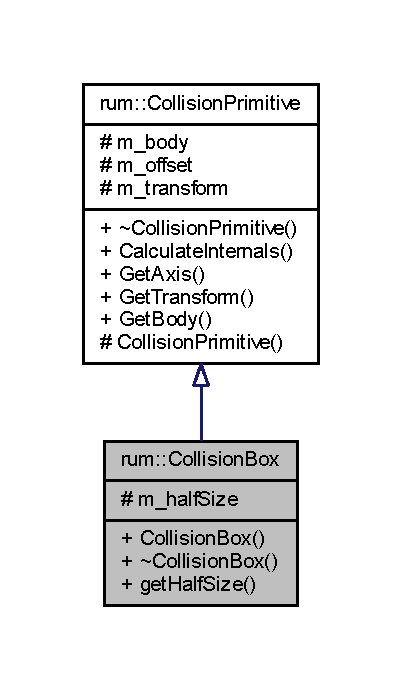
\includegraphics[width=193pt]{classrum_1_1_collision_box__inherit__graph}
\end{center}
\end{figure}


Collaboration diagram for rum\+:\+:Collision\+Box\+:\nopagebreak
\begin{figure}[H]
\begin{center}
\leavevmode
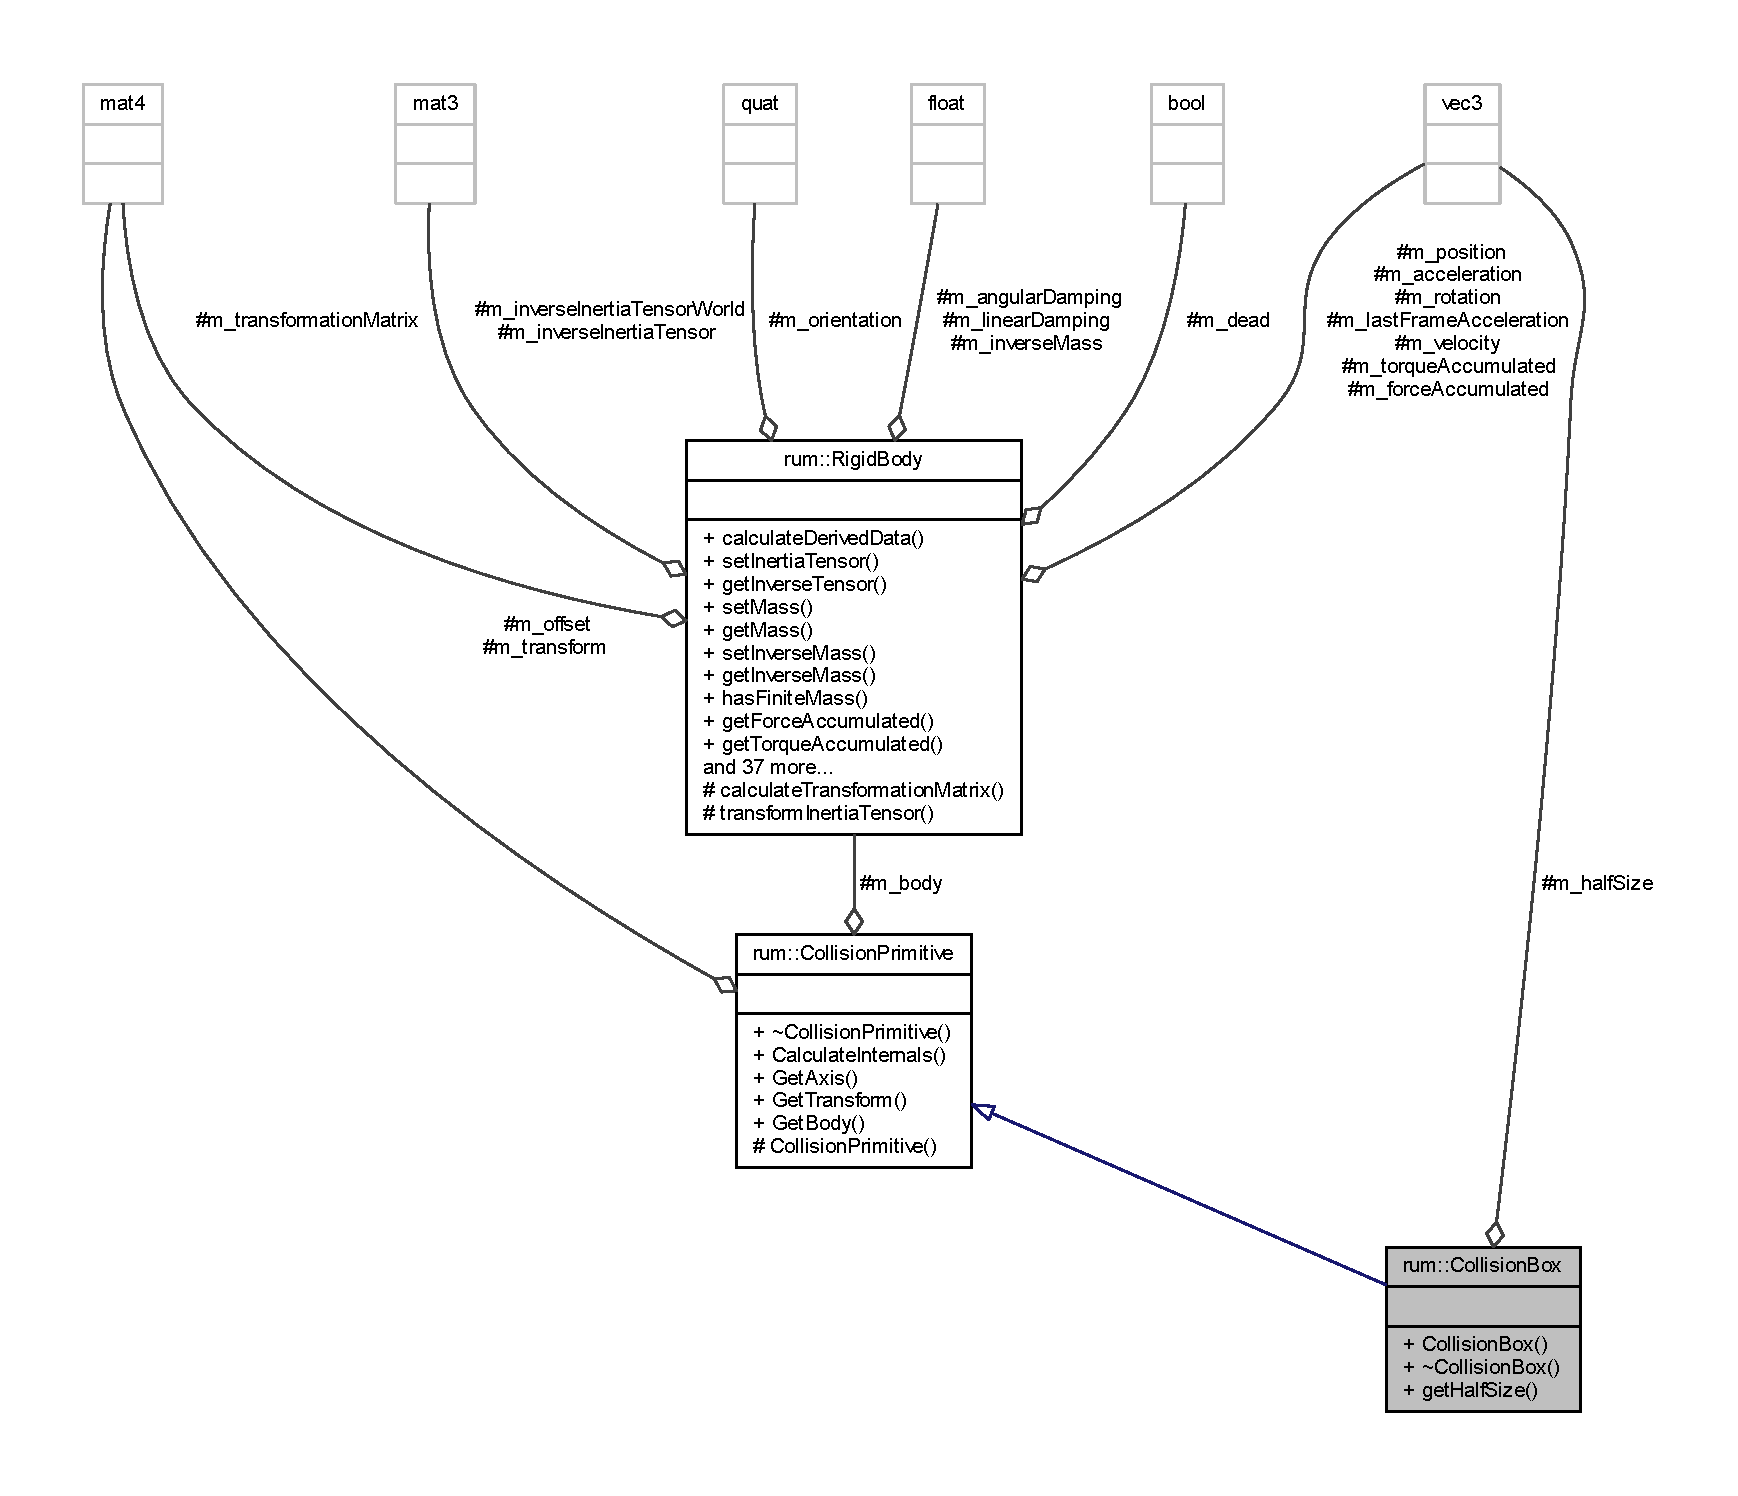
\includegraphics[width=350pt]{classrum_1_1_collision_box__coll__graph}
\end{center}
\end{figure}
\subsection*{Public Member Functions}
\begin{DoxyCompactItemize}
\item 
\mbox{\hyperlink{classrum_1_1_collision_box_a8b829760e2fb5c6ae02753067e0575d5}{Collision\+Box}} (\mbox{\hyperlink{classrum_1_1_rigid_body}{Rigid\+Body}} $\ast$body, const glm\+::mat4 \&offset, const glm\+::vec3 \&half\+Size)
\item 
\mbox{\hyperlink{classrum_1_1_collision_box_a3e480bda7dc21dad54dbc18bf38a7da3}{$\sim$\+Collision\+Box}} ()
\item 
glm\+::vec3 \mbox{\hyperlink{classrum_1_1_collision_box_a41fd485b6fc134f77a83efba31f19543}{get\+Half\+Size}} () const
\item 
void \mbox{\hyperlink{classrum_1_1_collision_box_a3f72c354e24f866be640f0b3f8e2a4b4}{generate\+Contact}} (\mbox{\hyperlink{classrum_1_1_i_narrow_phase_filter}{I\+Narrow\+Phase\+Filter}} $\ast$filter, \mbox{\hyperlink{classrum_1_1_collision_primitive}{Collision\+Primitive}} $\ast$other) override
\end{DoxyCompactItemize}
\subsection*{Protected Attributes}
\begin{DoxyCompactItemize}
\item 
glm\+::vec3 \mbox{\hyperlink{classrum_1_1_collision_box_ac154420e43adf96a09bd6d1340987bb5}{m\+\_\+half\+Size}}
\end{DoxyCompactItemize}
\subsection*{Additional Inherited Members}


\subsection{Constructor \& Destructor Documentation}
\mbox{\Hypertarget{classrum_1_1_collision_box_a8b829760e2fb5c6ae02753067e0575d5}\label{classrum_1_1_collision_box_a8b829760e2fb5c6ae02753067e0575d5}} 
\index{rum\+::\+Collision\+Box@{rum\+::\+Collision\+Box}!Collision\+Box@{Collision\+Box}}
\index{Collision\+Box@{Collision\+Box}!rum\+::\+Collision\+Box@{rum\+::\+Collision\+Box}}
\subsubsection{\texorpdfstring{Collision\+Box()}{CollisionBox()}}
{\footnotesize\ttfamily rum\+::\+Collision\+Box\+::\+Collision\+Box (\begin{DoxyParamCaption}\item[{\mbox{\hyperlink{classrum_1_1_rigid_body}{Rigid\+Body}} $\ast$}]{body,  }\item[{const glm\+::mat4 \&}]{offset,  }\item[{const glm\+::vec3 \&}]{half\+Size }\end{DoxyParamCaption})\hspace{0.3cm}{\ttfamily [explicit]}}

\mbox{\Hypertarget{classrum_1_1_collision_box_a3e480bda7dc21dad54dbc18bf38a7da3}\label{classrum_1_1_collision_box_a3e480bda7dc21dad54dbc18bf38a7da3}} 
\index{rum\+::\+Collision\+Box@{rum\+::\+Collision\+Box}!````~Collision\+Box@{$\sim$\+Collision\+Box}}
\index{````~Collision\+Box@{$\sim$\+Collision\+Box}!rum\+::\+Collision\+Box@{rum\+::\+Collision\+Box}}
\subsubsection{\texorpdfstring{$\sim$\+Collision\+Box()}{~CollisionBox()}}
{\footnotesize\ttfamily rum\+::\+Collision\+Box\+::$\sim$\+Collision\+Box (\begin{DoxyParamCaption}{ }\end{DoxyParamCaption})\hspace{0.3cm}{\ttfamily [default]}}



\subsection{Member Function Documentation}
\mbox{\Hypertarget{classrum_1_1_collision_box_a3f72c354e24f866be640f0b3f8e2a4b4}\label{classrum_1_1_collision_box_a3f72c354e24f866be640f0b3f8e2a4b4}} 
\index{rum\+::\+Collision\+Box@{rum\+::\+Collision\+Box}!generate\+Contact@{generate\+Contact}}
\index{generate\+Contact@{generate\+Contact}!rum\+::\+Collision\+Box@{rum\+::\+Collision\+Box}}
\subsubsection{\texorpdfstring{generate\+Contact()}{generateContact()}}
{\footnotesize\ttfamily void rum\+::\+Collision\+Box\+::generate\+Contact (\begin{DoxyParamCaption}\item[{\mbox{\hyperlink{classrum_1_1_i_narrow_phase_filter}{I\+Narrow\+Phase\+Filter}} $\ast$}]{filter,  }\item[{\mbox{\hyperlink{classrum_1_1_collision_primitive}{Collision\+Primitive}} $\ast$}]{other }\end{DoxyParamCaption})\hspace{0.3cm}{\ttfamily [override]}, {\ttfamily [virtual]}}



Implements \mbox{\hyperlink{classrum_1_1_collision_primitive_a31af51e97485378954de219b8411a27d}{rum\+::\+Collision\+Primitive}}.

\mbox{\Hypertarget{classrum_1_1_collision_box_a41fd485b6fc134f77a83efba31f19543}\label{classrum_1_1_collision_box_a41fd485b6fc134f77a83efba31f19543}} 
\index{rum\+::\+Collision\+Box@{rum\+::\+Collision\+Box}!get\+Half\+Size@{get\+Half\+Size}}
\index{get\+Half\+Size@{get\+Half\+Size}!rum\+::\+Collision\+Box@{rum\+::\+Collision\+Box}}
\subsubsection{\texorpdfstring{get\+Half\+Size()}{getHalfSize()}}
{\footnotesize\ttfamily glm\+::vec3 rum\+::\+Collision\+Box\+::get\+Half\+Size (\begin{DoxyParamCaption}{ }\end{DoxyParamCaption}) const}



\subsection{Member Data Documentation}
\mbox{\Hypertarget{classrum_1_1_collision_box_ac154420e43adf96a09bd6d1340987bb5}\label{classrum_1_1_collision_box_ac154420e43adf96a09bd6d1340987bb5}} 
\index{rum\+::\+Collision\+Box@{rum\+::\+Collision\+Box}!m\+\_\+half\+Size@{m\+\_\+half\+Size}}
\index{m\+\_\+half\+Size@{m\+\_\+half\+Size}!rum\+::\+Collision\+Box@{rum\+::\+Collision\+Box}}
\subsubsection{\texorpdfstring{m\+\_\+half\+Size}{m\_halfSize}}
{\footnotesize\ttfamily glm\+::vec3 rum\+::\+Collision\+Box\+::m\+\_\+half\+Size\hspace{0.3cm}{\ttfamily [protected]}}



The documentation for this class was generated from the following files\+:\begin{DoxyCompactItemize}
\item 
D\+:/\+Library/\+Documents/\+Job/\+Forschungsmaster/\+Projekte/\+Rumble3\+D/\+Rumble3\+D/include/\+R3\+D/\+Rigid\+Body\+Engine/\mbox{\hyperlink{_collision_box_8h}{Collision\+Box.\+h}}\item 
D\+:/\+Library/\+Documents/\+Job/\+Forschungsmaster/\+Projekte/\+Rumble3\+D/\+Rumble3\+D/src/\+Rigid\+Body\+Engine/\mbox{\hyperlink{_collision_box_8cpp}{Collision\+Box.\+cpp}}\end{DoxyCompactItemize}

\hypertarget{classrum_1_1_collision_data}{}\section{rum\+:\+:Collision\+Data Class Reference}
\label{classrum_1_1_collision_data}\index{rum\+::\+Collision\+Data@{rum\+::\+Collision\+Data}}


{\ttfamily \#include $<$Collision\+Data.\+h$>$}



Collaboration diagram for rum\+:\+:Collision\+Data\+:\nopagebreak
\begin{figure}[H]
\begin{center}
\leavevmode
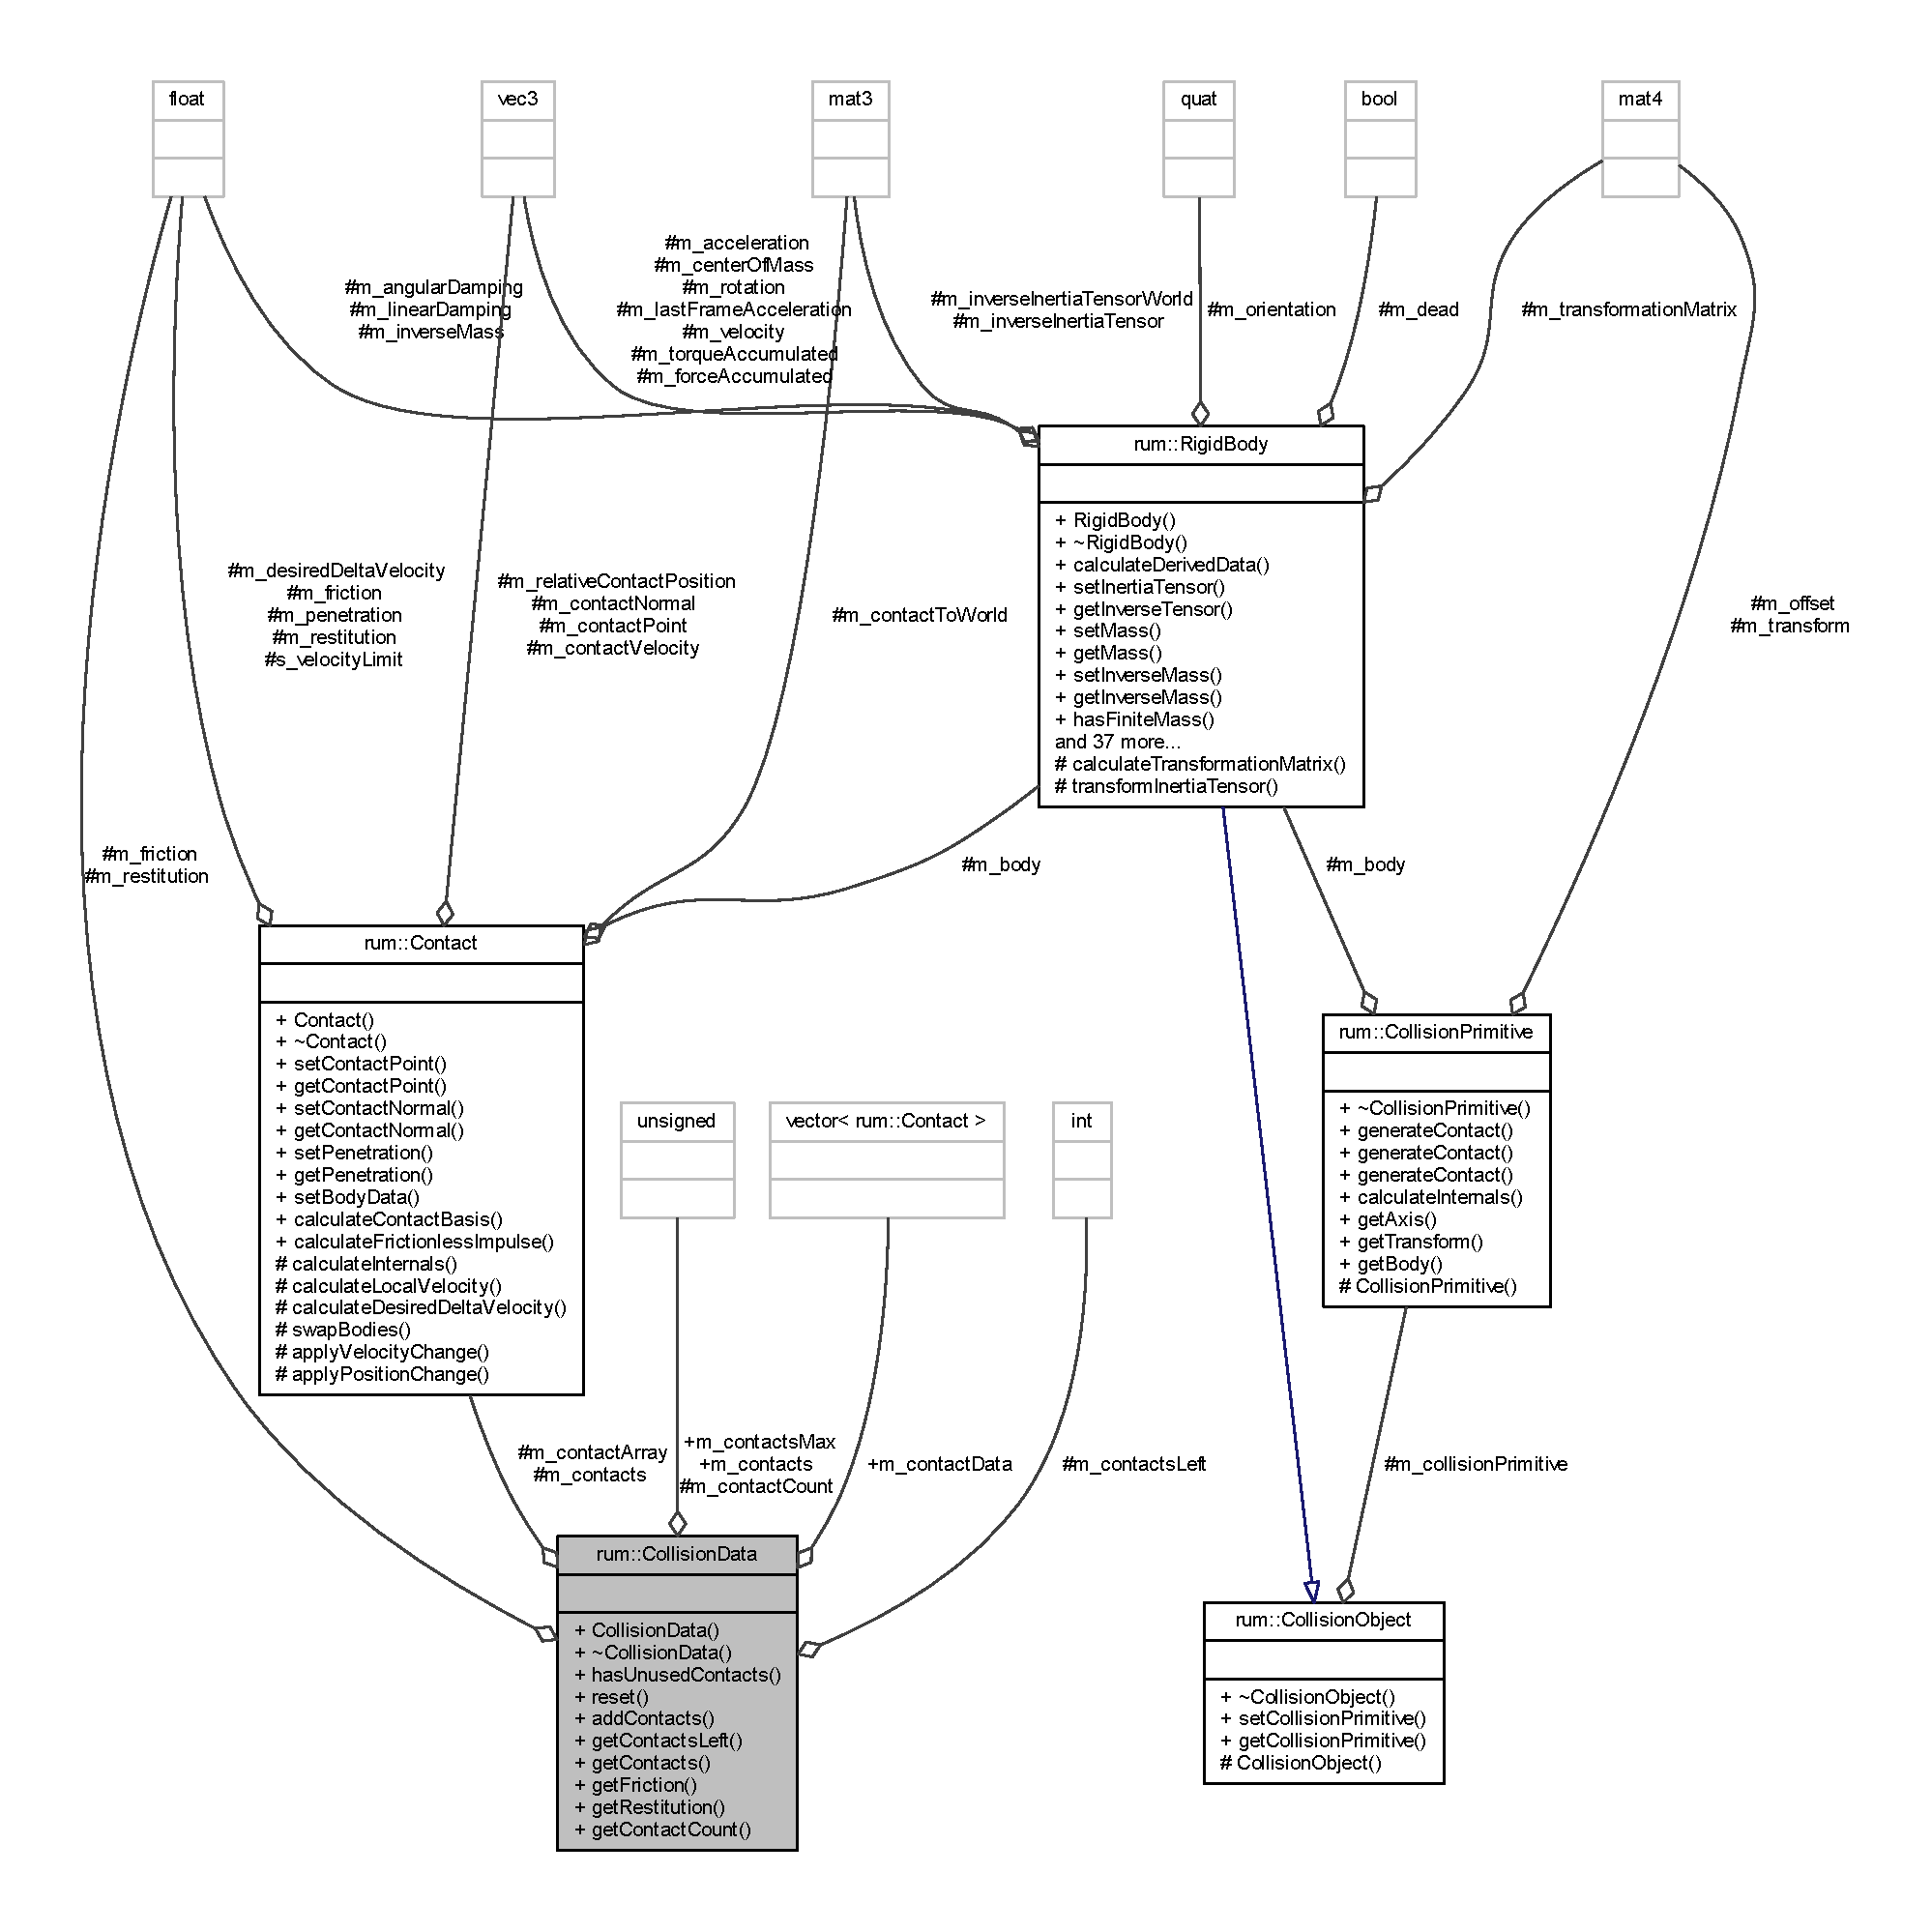
\includegraphics[width=350pt]{classrum_1_1_collision_data__coll__graph}
\end{center}
\end{figure}
\subsection*{Public Member Functions}
\begin{DoxyCompactItemize}
\item 
bool \hyperlink{classrum_1_1_collision_data_acbe7735f5186b368900f7c68ca2d7b4f}{has\+More\+Contacts} ()
\item 
void \hyperlink{classrum_1_1_collision_data_ae49fabbf40a855eab3ce0003aa418253}{reset} (unsigned max\+Contacts)
\item 
void \hyperlink{classrum_1_1_collision_data_a6774145a5f81c49c30c5d0c7954d35d5}{add\+Contacts} (unsigned count)
\item 
int \hyperlink{classrum_1_1_collision_data_a2b3dcbec102ae7affab46ba19c7c4eb7}{get\+Contacts\+Left} () const
\item 
\hyperlink{classrum_1_1_contact}{Contact} $\ast$ \hyperlink{classrum_1_1_collision_data_a0b9d69450fbefbb28b0d427793cccc26}{get\+Contacts} () const
\item 
\hyperlink{namespacerum_a7e8cca23573d5eaead0f138cbaa4862c}{real} \hyperlink{classrum_1_1_collision_data_a917290357ac710e3d4e1bfce4d040495}{get\+Friction} () const
\item 
\hyperlink{namespacerum_a7e8cca23573d5eaead0f138cbaa4862c}{real} \hyperlink{classrum_1_1_collision_data_aae54080198ebe0e4700142f0ad03b344}{get\+Restitution} () const
\item 
int \hyperlink{classrum_1_1_collision_data_a77b0f7209d6709f8a2041722428f56d5}{get\+Contact\+Count} () const
\end{DoxyCompactItemize}
\subsection*{Protected Attributes}
\begin{DoxyCompactItemize}
\item 
\hyperlink{classrum_1_1_contact}{Contact} $\ast$ \hyperlink{classrum_1_1_collision_data_a81c91a3b806491ce9a6c2b458e10cee6}{m\+\_\+contact\+Array}
\item 
\hyperlink{classrum_1_1_contact}{Contact} $\ast$ \hyperlink{classrum_1_1_collision_data_a4328ce35ae3759b3ca313177bb561ef0}{m\+\_\+contacts}
\item 
int \hyperlink{classrum_1_1_collision_data_a037132e6e4f65c885f1d29da338df4af}{m\+\_\+contacts\+Left}
\item 
unsigned \hyperlink{classrum_1_1_collision_data_a17225794f1a582d0d5c5565ffc3334ff}{m\+\_\+contact\+Count}
\item 
\hyperlink{namespacerum_a7e8cca23573d5eaead0f138cbaa4862c}{real} \hyperlink{classrum_1_1_collision_data_a752a7564c13eeff1a03b6552238f6a00}{m\+\_\+friction} = 0.\+5f
\item 
\hyperlink{namespacerum_a7e8cca23573d5eaead0f138cbaa4862c}{real} \hyperlink{classrum_1_1_collision_data_ab28c985d5b8554f548a485cac367c1fd}{m\+\_\+restitution} = 0.\+5f
\end{DoxyCompactItemize}


\subsection{Member Function Documentation}
\mbox{\Hypertarget{classrum_1_1_collision_data_a6774145a5f81c49c30c5d0c7954d35d5}\label{classrum_1_1_collision_data_a6774145a5f81c49c30c5d0c7954d35d5}} 
\index{rum\+::\+Collision\+Data@{rum\+::\+Collision\+Data}!add\+Contacts@{add\+Contacts}}
\index{add\+Contacts@{add\+Contacts}!rum\+::\+Collision\+Data@{rum\+::\+Collision\+Data}}
\subsubsection{\texorpdfstring{add\+Contacts()}{addContacts()}}
{\footnotesize\ttfamily void rum\+::\+Collision\+Data\+::add\+Contacts (\begin{DoxyParamCaption}\item[{unsigned}]{count }\end{DoxyParamCaption})}

\mbox{\Hypertarget{classrum_1_1_collision_data_a77b0f7209d6709f8a2041722428f56d5}\label{classrum_1_1_collision_data_a77b0f7209d6709f8a2041722428f56d5}} 
\index{rum\+::\+Collision\+Data@{rum\+::\+Collision\+Data}!get\+Contact\+Count@{get\+Contact\+Count}}
\index{get\+Contact\+Count@{get\+Contact\+Count}!rum\+::\+Collision\+Data@{rum\+::\+Collision\+Data}}
\subsubsection{\texorpdfstring{get\+Contact\+Count()}{getContactCount()}}
{\footnotesize\ttfamily int rum\+::\+Collision\+Data\+::get\+Contact\+Count (\begin{DoxyParamCaption}{ }\end{DoxyParamCaption}) const}

\mbox{\Hypertarget{classrum_1_1_collision_data_a0b9d69450fbefbb28b0d427793cccc26}\label{classrum_1_1_collision_data_a0b9d69450fbefbb28b0d427793cccc26}} 
\index{rum\+::\+Collision\+Data@{rum\+::\+Collision\+Data}!get\+Contacts@{get\+Contacts}}
\index{get\+Contacts@{get\+Contacts}!rum\+::\+Collision\+Data@{rum\+::\+Collision\+Data}}
\subsubsection{\texorpdfstring{get\+Contacts()}{getContacts()}}
{\footnotesize\ttfamily \hyperlink{classrum_1_1_contact}{Contact} $\ast$ rum\+::\+Collision\+Data\+::get\+Contacts (\begin{DoxyParamCaption}{ }\end{DoxyParamCaption}) const}

\mbox{\Hypertarget{classrum_1_1_collision_data_a2b3dcbec102ae7affab46ba19c7c4eb7}\label{classrum_1_1_collision_data_a2b3dcbec102ae7affab46ba19c7c4eb7}} 
\index{rum\+::\+Collision\+Data@{rum\+::\+Collision\+Data}!get\+Contacts\+Left@{get\+Contacts\+Left}}
\index{get\+Contacts\+Left@{get\+Contacts\+Left}!rum\+::\+Collision\+Data@{rum\+::\+Collision\+Data}}
\subsubsection{\texorpdfstring{get\+Contacts\+Left()}{getContactsLeft()}}
{\footnotesize\ttfamily int rum\+::\+Collision\+Data\+::get\+Contacts\+Left (\begin{DoxyParamCaption}{ }\end{DoxyParamCaption}) const}

\mbox{\Hypertarget{classrum_1_1_collision_data_a917290357ac710e3d4e1bfce4d040495}\label{classrum_1_1_collision_data_a917290357ac710e3d4e1bfce4d040495}} 
\index{rum\+::\+Collision\+Data@{rum\+::\+Collision\+Data}!get\+Friction@{get\+Friction}}
\index{get\+Friction@{get\+Friction}!rum\+::\+Collision\+Data@{rum\+::\+Collision\+Data}}
\subsubsection{\texorpdfstring{get\+Friction()}{getFriction()}}
{\footnotesize\ttfamily \hyperlink{namespacerum_a7e8cca23573d5eaead0f138cbaa4862c}{real} rum\+::\+Collision\+Data\+::get\+Friction (\begin{DoxyParamCaption}{ }\end{DoxyParamCaption}) const}

\mbox{\Hypertarget{classrum_1_1_collision_data_aae54080198ebe0e4700142f0ad03b344}\label{classrum_1_1_collision_data_aae54080198ebe0e4700142f0ad03b344}} 
\index{rum\+::\+Collision\+Data@{rum\+::\+Collision\+Data}!get\+Restitution@{get\+Restitution}}
\index{get\+Restitution@{get\+Restitution}!rum\+::\+Collision\+Data@{rum\+::\+Collision\+Data}}
\subsubsection{\texorpdfstring{get\+Restitution()}{getRestitution()}}
{\footnotesize\ttfamily \hyperlink{namespacerum_a7e8cca23573d5eaead0f138cbaa4862c}{real} rum\+::\+Collision\+Data\+::get\+Restitution (\begin{DoxyParamCaption}{ }\end{DoxyParamCaption}) const}

\mbox{\Hypertarget{classrum_1_1_collision_data_acbe7735f5186b368900f7c68ca2d7b4f}\label{classrum_1_1_collision_data_acbe7735f5186b368900f7c68ca2d7b4f}} 
\index{rum\+::\+Collision\+Data@{rum\+::\+Collision\+Data}!has\+More\+Contacts@{has\+More\+Contacts}}
\index{has\+More\+Contacts@{has\+More\+Contacts}!rum\+::\+Collision\+Data@{rum\+::\+Collision\+Data}}
\subsubsection{\texorpdfstring{has\+More\+Contacts()}{hasMoreContacts()}}
{\footnotesize\ttfamily bool rum\+::\+Collision\+Data\+::has\+More\+Contacts (\begin{DoxyParamCaption}{ }\end{DoxyParamCaption})}

\mbox{\Hypertarget{classrum_1_1_collision_data_ae49fabbf40a855eab3ce0003aa418253}\label{classrum_1_1_collision_data_ae49fabbf40a855eab3ce0003aa418253}} 
\index{rum\+::\+Collision\+Data@{rum\+::\+Collision\+Data}!reset@{reset}}
\index{reset@{reset}!rum\+::\+Collision\+Data@{rum\+::\+Collision\+Data}}
\subsubsection{\texorpdfstring{reset()}{reset()}}
{\footnotesize\ttfamily void rum\+::\+Collision\+Data\+::reset (\begin{DoxyParamCaption}\item[{unsigned}]{max\+Contacts }\end{DoxyParamCaption})}



\subsection{Member Data Documentation}
\mbox{\Hypertarget{classrum_1_1_collision_data_a81c91a3b806491ce9a6c2b458e10cee6}\label{classrum_1_1_collision_data_a81c91a3b806491ce9a6c2b458e10cee6}} 
\index{rum\+::\+Collision\+Data@{rum\+::\+Collision\+Data}!m\+\_\+contact\+Array@{m\+\_\+contact\+Array}}
\index{m\+\_\+contact\+Array@{m\+\_\+contact\+Array}!rum\+::\+Collision\+Data@{rum\+::\+Collision\+Data}}
\subsubsection{\texorpdfstring{m\+\_\+contact\+Array}{m\_contactArray}}
{\footnotesize\ttfamily \hyperlink{classrum_1_1_contact}{Contact}$\ast$ rum\+::\+Collision\+Data\+::m\+\_\+contact\+Array\hspace{0.3cm}{\ttfamily [protected]}}

\mbox{\Hypertarget{classrum_1_1_collision_data_a17225794f1a582d0d5c5565ffc3334ff}\label{classrum_1_1_collision_data_a17225794f1a582d0d5c5565ffc3334ff}} 
\index{rum\+::\+Collision\+Data@{rum\+::\+Collision\+Data}!m\+\_\+contact\+Count@{m\+\_\+contact\+Count}}
\index{m\+\_\+contact\+Count@{m\+\_\+contact\+Count}!rum\+::\+Collision\+Data@{rum\+::\+Collision\+Data}}
\subsubsection{\texorpdfstring{m\+\_\+contact\+Count}{m\_contactCount}}
{\footnotesize\ttfamily unsigned rum\+::\+Collision\+Data\+::m\+\_\+contact\+Count\hspace{0.3cm}{\ttfamily [protected]}}

\mbox{\Hypertarget{classrum_1_1_collision_data_a4328ce35ae3759b3ca313177bb561ef0}\label{classrum_1_1_collision_data_a4328ce35ae3759b3ca313177bb561ef0}} 
\index{rum\+::\+Collision\+Data@{rum\+::\+Collision\+Data}!m\+\_\+contacts@{m\+\_\+contacts}}
\index{m\+\_\+contacts@{m\+\_\+contacts}!rum\+::\+Collision\+Data@{rum\+::\+Collision\+Data}}
\subsubsection{\texorpdfstring{m\+\_\+contacts}{m\_contacts}}
{\footnotesize\ttfamily \hyperlink{classrum_1_1_contact}{Contact}$\ast$ rum\+::\+Collision\+Data\+::m\+\_\+contacts\hspace{0.3cm}{\ttfamily [protected]}}

\mbox{\Hypertarget{classrum_1_1_collision_data_a037132e6e4f65c885f1d29da338df4af}\label{classrum_1_1_collision_data_a037132e6e4f65c885f1d29da338df4af}} 
\index{rum\+::\+Collision\+Data@{rum\+::\+Collision\+Data}!m\+\_\+contacts\+Left@{m\+\_\+contacts\+Left}}
\index{m\+\_\+contacts\+Left@{m\+\_\+contacts\+Left}!rum\+::\+Collision\+Data@{rum\+::\+Collision\+Data}}
\subsubsection{\texorpdfstring{m\+\_\+contacts\+Left}{m\_contactsLeft}}
{\footnotesize\ttfamily int rum\+::\+Collision\+Data\+::m\+\_\+contacts\+Left\hspace{0.3cm}{\ttfamily [protected]}}

\mbox{\Hypertarget{classrum_1_1_collision_data_a752a7564c13eeff1a03b6552238f6a00}\label{classrum_1_1_collision_data_a752a7564c13eeff1a03b6552238f6a00}} 
\index{rum\+::\+Collision\+Data@{rum\+::\+Collision\+Data}!m\+\_\+friction@{m\+\_\+friction}}
\index{m\+\_\+friction@{m\+\_\+friction}!rum\+::\+Collision\+Data@{rum\+::\+Collision\+Data}}
\subsubsection{\texorpdfstring{m\+\_\+friction}{m\_friction}}
{\footnotesize\ttfamily \hyperlink{namespacerum_a7e8cca23573d5eaead0f138cbaa4862c}{real} rum\+::\+Collision\+Data\+::m\+\_\+friction = 0.\+5f\hspace{0.3cm}{\ttfamily [protected]}}

\mbox{\Hypertarget{classrum_1_1_collision_data_ab28c985d5b8554f548a485cac367c1fd}\label{classrum_1_1_collision_data_ab28c985d5b8554f548a485cac367c1fd}} 
\index{rum\+::\+Collision\+Data@{rum\+::\+Collision\+Data}!m\+\_\+restitution@{m\+\_\+restitution}}
\index{m\+\_\+restitution@{m\+\_\+restitution}!rum\+::\+Collision\+Data@{rum\+::\+Collision\+Data}}
\subsubsection{\texorpdfstring{m\+\_\+restitution}{m\_restitution}}
{\footnotesize\ttfamily \hyperlink{namespacerum_a7e8cca23573d5eaead0f138cbaa4862c}{real} rum\+::\+Collision\+Data\+::m\+\_\+restitution = 0.\+5f\hspace{0.3cm}{\ttfamily [protected]}}



The documentation for this class was generated from the following files\+:\begin{DoxyCompactItemize}
\item 
F\+:/\+Library/\+Documents/\+Job/\+Forschungsmaster/\+Rumble3\+D/\+Rumble3\+D/include/\+R3\+D/\+Rigid\+Body\+Engine/\hyperlink{_collision_data_8h}{Collision\+Data.\+h}\item 
F\+:/\+Library/\+Documents/\+Job/\+Forschungsmaster/\+Rumble3\+D/\+Rumble3\+D/src/\+Rigid\+Body\+Engine/\hyperlink{_collision_data_8cpp}{Collision\+Data.\+cpp}\end{DoxyCompactItemize}

\hypertarget{classrum_1_1_collision_detector}{}\section{rum\+:\+:Collision\+Detector Class Reference}
\label{classrum_1_1_collision_detector}\index{rum\+::\+Collision\+Detector@{rum\+::\+Collision\+Detector}}


{\ttfamily \#include $<$Collision\+Detector.\+h$>$}



Collaboration diagram for rum\+:\+:Collision\+Detector\+:\nopagebreak
\begin{figure}[H]
\begin{center}
\leavevmode
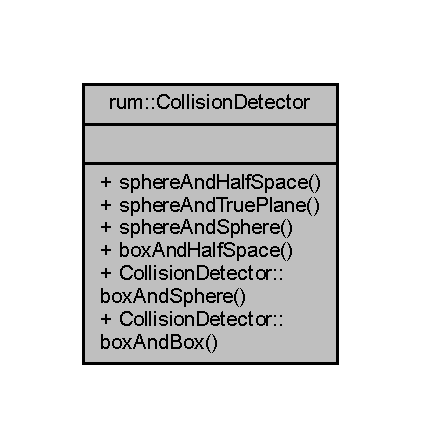
\includegraphics[width=245pt]{classrum_1_1_collision_detector__coll__graph}
\end{center}
\end{figure}
\subsection*{Public Types}
\begin{DoxyCompactItemize}
\item 
using \mbox{\hyperlink{classrum_1_1_collision_detector_a76f794d3db7491b5b21137c6332eccb3}{Broad\+Phase\+Filter\+\_\+\+Ptr}} = std\+::unique\+\_\+ptr$<$ \mbox{\hyperlink{classrum_1_1_i_broad_phase_filter}{I\+Broad\+Phase\+Filter}} $>$
\item 
using \mbox{\hyperlink{classrum_1_1_collision_detector_aa1a7155543cdbe0265865b3e6f14b260}{Intermediate\+Phase\+Filter\+\_\+\+Ptr}} = std\+::unique\+\_\+ptr$<$ \mbox{\hyperlink{classrum_1_1_i_intermediate_phase_filter}{I\+Intermediate\+Phase\+Filter}} $>$
\item 
using \mbox{\hyperlink{classrum_1_1_collision_detector_a8a6d24fed38f8be11b25e43eaabc9638}{Narrow\+Phase\+Filter\+\_\+\+Ptr}} = std\+::unique\+\_\+ptr$<$ \mbox{\hyperlink{classrum_1_1_i_narrow_phase_filter}{I\+Narrow\+Phase\+Filter}} $>$
\end{DoxyCompactItemize}
\subsection*{Public Member Functions}
\begin{DoxyCompactItemize}
\item 
\mbox{\hyperlink{classrum_1_1_collision_detector_a5547ad2cf2a42536f8d653405bbb6485}{Collision\+Detector}} (unsigned int iterations=10, unsigned int contacts\+Max=1000)
\item 
\mbox{\hyperlink{classrum_1_1_collision_detector_a55d704761a707ed6a8a6842f3d5058b5}{Collision\+Detector}} (const \mbox{\hyperlink{classrum_1_1_collision_detector}{Collision\+Detector}} \&)=delete
\item 
\mbox{\hyperlink{classrum_1_1_collision_detector_a9bf8f0c5853254f4a905879ab0187858}{$\sim$\+Collision\+Detector}} ()
\item 
const \mbox{\hyperlink{classrum_1_1_collision_data}{Collision\+Data}} \& \mbox{\hyperlink{classrum_1_1_collision_detector_aa8096b4bb5f7b6ebf1605202ef170734}{generate\+Collisions}} (const std\+::vector$<$ \mbox{\hyperlink{classrum_1_1_rigid_body}{Rigid\+Body}} $\ast$$>$ \&rigid\+Bodies)
\item 
void \mbox{\hyperlink{classrum_1_1_collision_detector_aa79501a56911cc6ea64e53278bedb2cb}{set\+Broad\+Phase\+Filter}} (\mbox{\hyperlink{classrum_1_1_collision_detector_a76f794d3db7491b5b21137c6332eccb3}{Broad\+Phase\+Filter\+\_\+\+Ptr}} filter)
\item 
\mbox{\hyperlink{classrum_1_1_i_broad_phase_filter}{I\+Broad\+Phase\+Filter}} $\ast$ \mbox{\hyperlink{classrum_1_1_collision_detector_aa03aaf950039ff0cac3013c8b23ed8d6}{get\+Broad\+Phase\+Filter}} () const
\item 
\mbox{\hyperlink{classrum_1_1_i_intermediate_phase_filter}{I\+Intermediate\+Phase\+Filter}} $\ast$ \mbox{\hyperlink{classrum_1_1_collision_detector_ac94d9993483834effa1baea4ca938ad3}{add\+Intermediate\+Phase\+Filter}} (\mbox{\hyperlink{classrum_1_1_collision_detector_aa1a7155543cdbe0265865b3e6f14b260}{Intermediate\+Phase\+Filter\+\_\+\+Ptr}} filter)
\item 
\mbox{\hyperlink{classrum_1_1_collision_detector_aa1a7155543cdbe0265865b3e6f14b260}{Intermediate\+Phase\+Filter\+\_\+\+Ptr}} \mbox{\hyperlink{classrum_1_1_collision_detector_a94446ddd3ad221a5403288f91fc538d9}{remove\+Intermediate\+Phase\+Filter}} (\mbox{\hyperlink{classrum_1_1_i_intermediate_phase_filter}{I\+Intermediate\+Phase\+Filter}} $\ast$filter)
\item 
void \mbox{\hyperlink{classrum_1_1_collision_detector_a378bc34c76126678e5ad0ef801d9a0d6}{remove\+All\+Intermediate\+Phase\+Filters}} ()
\item 
void \mbox{\hyperlink{classrum_1_1_collision_detector_ae81fd3b892eb3a03520b6487ae91dedd}{set\+Narrow\+Phase\+Filter}} (\mbox{\hyperlink{classrum_1_1_collision_detector_a8a6d24fed38f8be11b25e43eaabc9638}{Narrow\+Phase\+Filter\+\_\+\+Ptr}} filter)
\item 
\mbox{\hyperlink{classrum_1_1_i_narrow_phase_filter}{I\+Narrow\+Phase\+Filter}} $\ast$ \mbox{\hyperlink{classrum_1_1_collision_detector_a804d2926d30afa1e45629643b1262b64}{get\+Narrow\+Phase\+Filter}} () const
\end{DoxyCompactItemize}


\subsection{Detailed Description}
The \mbox{\hyperlink{classrum_1_1_collision_detector}{Collision\+Detector}} acts as a batch controller (batch sequential). It executes collision detection filters (programs) in a specific order to generate contacts. 

\subsection{Member Typedef Documentation}
\mbox{\Hypertarget{classrum_1_1_collision_detector_a76f794d3db7491b5b21137c6332eccb3}\label{classrum_1_1_collision_detector_a76f794d3db7491b5b21137c6332eccb3}} 
\index{rum\+::\+Collision\+Detector@{rum\+::\+Collision\+Detector}!Broad\+Phase\+Filter\+\_\+\+Ptr@{Broad\+Phase\+Filter\+\_\+\+Ptr}}
\index{Broad\+Phase\+Filter\+\_\+\+Ptr@{Broad\+Phase\+Filter\+\_\+\+Ptr}!rum\+::\+Collision\+Detector@{rum\+::\+Collision\+Detector}}
\subsubsection{\texorpdfstring{Broad\+Phase\+Filter\+\_\+\+Ptr}{BroadPhaseFilter\_Ptr}}
{\footnotesize\ttfamily using \mbox{\hyperlink{classrum_1_1_collision_detector_a76f794d3db7491b5b21137c6332eccb3}{rum\+::\+Collision\+Detector\+::\+Broad\+Phase\+Filter\+\_\+\+Ptr}} =  std\+::unique\+\_\+ptr$<$\mbox{\hyperlink{classrum_1_1_i_broad_phase_filter}{I\+Broad\+Phase\+Filter}}$>$}

\mbox{\Hypertarget{classrum_1_1_collision_detector_aa1a7155543cdbe0265865b3e6f14b260}\label{classrum_1_1_collision_detector_aa1a7155543cdbe0265865b3e6f14b260}} 
\index{rum\+::\+Collision\+Detector@{rum\+::\+Collision\+Detector}!Intermediate\+Phase\+Filter\+\_\+\+Ptr@{Intermediate\+Phase\+Filter\+\_\+\+Ptr}}
\index{Intermediate\+Phase\+Filter\+\_\+\+Ptr@{Intermediate\+Phase\+Filter\+\_\+\+Ptr}!rum\+::\+Collision\+Detector@{rum\+::\+Collision\+Detector}}
\subsubsection{\texorpdfstring{Intermediate\+Phase\+Filter\+\_\+\+Ptr}{IntermediatePhaseFilter\_Ptr}}
{\footnotesize\ttfamily using \mbox{\hyperlink{classrum_1_1_collision_detector_aa1a7155543cdbe0265865b3e6f14b260}{rum\+::\+Collision\+Detector\+::\+Intermediate\+Phase\+Filter\+\_\+\+Ptr}} =  std\+::unique\+\_\+ptr$<$\mbox{\hyperlink{classrum_1_1_i_intermediate_phase_filter}{I\+Intermediate\+Phase\+Filter}}$>$}

\mbox{\Hypertarget{classrum_1_1_collision_detector_a8a6d24fed38f8be11b25e43eaabc9638}\label{classrum_1_1_collision_detector_a8a6d24fed38f8be11b25e43eaabc9638}} 
\index{rum\+::\+Collision\+Detector@{rum\+::\+Collision\+Detector}!Narrow\+Phase\+Filter\+\_\+\+Ptr@{Narrow\+Phase\+Filter\+\_\+\+Ptr}}
\index{Narrow\+Phase\+Filter\+\_\+\+Ptr@{Narrow\+Phase\+Filter\+\_\+\+Ptr}!rum\+::\+Collision\+Detector@{rum\+::\+Collision\+Detector}}
\subsubsection{\texorpdfstring{Narrow\+Phase\+Filter\+\_\+\+Ptr}{NarrowPhaseFilter\_Ptr}}
{\footnotesize\ttfamily using \mbox{\hyperlink{classrum_1_1_collision_detector_a8a6d24fed38f8be11b25e43eaabc9638}{rum\+::\+Collision\+Detector\+::\+Narrow\+Phase\+Filter\+\_\+\+Ptr}} =  std\+::unique\+\_\+ptr$<$\mbox{\hyperlink{classrum_1_1_i_narrow_phase_filter}{I\+Narrow\+Phase\+Filter}}$>$}



\subsection{Constructor \& Destructor Documentation}
\mbox{\Hypertarget{classrum_1_1_collision_detector_a5547ad2cf2a42536f8d653405bbb6485}\label{classrum_1_1_collision_detector_a5547ad2cf2a42536f8d653405bbb6485}} 
\index{rum\+::\+Collision\+Detector@{rum\+::\+Collision\+Detector}!Collision\+Detector@{Collision\+Detector}}
\index{Collision\+Detector@{Collision\+Detector}!rum\+::\+Collision\+Detector@{rum\+::\+Collision\+Detector}}
\subsubsection{\texorpdfstring{Collision\+Detector()}{CollisionDetector()}\hspace{0.1cm}{\footnotesize\ttfamily [1/2]}}
{\footnotesize\ttfamily rum\+::\+Collision\+Detector\+::\+Collision\+Detector (\begin{DoxyParamCaption}\item[{unsigned int}]{iterations = {\ttfamily 10},  }\item[{unsigned int}]{contacts\+Max = {\ttfamily 1000} }\end{DoxyParamCaption})\hspace{0.3cm}{\ttfamily [explicit]}}

\mbox{\Hypertarget{classrum_1_1_collision_detector_a55d704761a707ed6a8a6842f3d5058b5}\label{classrum_1_1_collision_detector_a55d704761a707ed6a8a6842f3d5058b5}} 
\index{rum\+::\+Collision\+Detector@{rum\+::\+Collision\+Detector}!Collision\+Detector@{Collision\+Detector}}
\index{Collision\+Detector@{Collision\+Detector}!rum\+::\+Collision\+Detector@{rum\+::\+Collision\+Detector}}
\subsubsection{\texorpdfstring{Collision\+Detector()}{CollisionDetector()}\hspace{0.1cm}{\footnotesize\ttfamily [2/2]}}
{\footnotesize\ttfamily rum\+::\+Collision\+Detector\+::\+Collision\+Detector (\begin{DoxyParamCaption}\item[{const \mbox{\hyperlink{classrum_1_1_collision_detector}{Collision\+Detector}} \&}]{ }\end{DoxyParamCaption})\hspace{0.3cm}{\ttfamily [delete]}}

\mbox{\Hypertarget{classrum_1_1_collision_detector_a9bf8f0c5853254f4a905879ab0187858}\label{classrum_1_1_collision_detector_a9bf8f0c5853254f4a905879ab0187858}} 
\index{rum\+::\+Collision\+Detector@{rum\+::\+Collision\+Detector}!````~Collision\+Detector@{$\sim$\+Collision\+Detector}}
\index{````~Collision\+Detector@{$\sim$\+Collision\+Detector}!rum\+::\+Collision\+Detector@{rum\+::\+Collision\+Detector}}
\subsubsection{\texorpdfstring{$\sim$\+Collision\+Detector()}{~CollisionDetector()}}
{\footnotesize\ttfamily rum\+::\+Collision\+Detector\+::$\sim$\+Collision\+Detector (\begin{DoxyParamCaption}{ }\end{DoxyParamCaption})\hspace{0.3cm}{\ttfamily [default]}}



\subsection{Member Function Documentation}
\mbox{\Hypertarget{classrum_1_1_collision_detector_ac94d9993483834effa1baea4ca938ad3}\label{classrum_1_1_collision_detector_ac94d9993483834effa1baea4ca938ad3}} 
\index{rum\+::\+Collision\+Detector@{rum\+::\+Collision\+Detector}!add\+Intermediate\+Phase\+Filter@{add\+Intermediate\+Phase\+Filter}}
\index{add\+Intermediate\+Phase\+Filter@{add\+Intermediate\+Phase\+Filter}!rum\+::\+Collision\+Detector@{rum\+::\+Collision\+Detector}}
\subsubsection{\texorpdfstring{add\+Intermediate\+Phase\+Filter()}{addIntermediatePhaseFilter()}}
{\footnotesize\ttfamily \mbox{\hyperlink{classrum_1_1_i_intermediate_phase_filter}{I\+Intermediate\+Phase\+Filter}} $\ast$ rum\+::\+Collision\+Detector\+::add\+Intermediate\+Phase\+Filter (\begin{DoxyParamCaption}\item[{\mbox{\hyperlink{classrum_1_1_collision_detector_aa1a7155543cdbe0265865b3e6f14b260}{Intermediate\+Phase\+Filter\+\_\+\+Ptr}}}]{filter }\end{DoxyParamCaption})}

Add a new intermediate phase filter, which will be executed after all currently registered intermediate phase filters. \begin{DoxyReturn}{Returns}
The newly inserted intermediate phase filter. 
\end{DoxyReturn}
\mbox{\Hypertarget{classrum_1_1_collision_detector_aa8096b4bb5f7b6ebf1605202ef170734}\label{classrum_1_1_collision_detector_aa8096b4bb5f7b6ebf1605202ef170734}} 
\index{rum\+::\+Collision\+Detector@{rum\+::\+Collision\+Detector}!generate\+Collisions@{generate\+Collisions}}
\index{generate\+Collisions@{generate\+Collisions}!rum\+::\+Collision\+Detector@{rum\+::\+Collision\+Detector}}
\subsubsection{\texorpdfstring{generate\+Collisions()}{generateCollisions()}}
{\footnotesize\ttfamily const \mbox{\hyperlink{classrum_1_1_collision_data}{Collision\+Data}} \& rum\+::\+Collision\+Detector\+::generate\+Collisions (\begin{DoxyParamCaption}\item[{const std\+::vector$<$ \mbox{\hyperlink{classrum_1_1_rigid_body}{Rigid\+Body}} $\ast$$>$ \&}]{rigid\+Bodies }\end{DoxyParamCaption})}

Generate a number of contacts for the given rigid bodies with the help of the current filters. \mbox{\Hypertarget{classrum_1_1_collision_detector_aa03aaf950039ff0cac3013c8b23ed8d6}\label{classrum_1_1_collision_detector_aa03aaf950039ff0cac3013c8b23ed8d6}} 
\index{rum\+::\+Collision\+Detector@{rum\+::\+Collision\+Detector}!get\+Broad\+Phase\+Filter@{get\+Broad\+Phase\+Filter}}
\index{get\+Broad\+Phase\+Filter@{get\+Broad\+Phase\+Filter}!rum\+::\+Collision\+Detector@{rum\+::\+Collision\+Detector}}
\subsubsection{\texorpdfstring{get\+Broad\+Phase\+Filter()}{getBroadPhaseFilter()}}
{\footnotesize\ttfamily \mbox{\hyperlink{classrum_1_1_i_broad_phase_filter}{I\+Broad\+Phase\+Filter}} $\ast$ rum\+::\+Collision\+Detector\+::get\+Broad\+Phase\+Filter (\begin{DoxyParamCaption}{ }\end{DoxyParamCaption}) const}

Get the currently used broad phase filter. \mbox{\Hypertarget{classrum_1_1_collision_detector_a804d2926d30afa1e45629643b1262b64}\label{classrum_1_1_collision_detector_a804d2926d30afa1e45629643b1262b64}} 
\index{rum\+::\+Collision\+Detector@{rum\+::\+Collision\+Detector}!get\+Narrow\+Phase\+Filter@{get\+Narrow\+Phase\+Filter}}
\index{get\+Narrow\+Phase\+Filter@{get\+Narrow\+Phase\+Filter}!rum\+::\+Collision\+Detector@{rum\+::\+Collision\+Detector}}
\subsubsection{\texorpdfstring{get\+Narrow\+Phase\+Filter()}{getNarrowPhaseFilter()}}
{\footnotesize\ttfamily \mbox{\hyperlink{classrum_1_1_i_narrow_phase_filter}{I\+Narrow\+Phase\+Filter}} $\ast$ rum\+::\+Collision\+Detector\+::get\+Narrow\+Phase\+Filter (\begin{DoxyParamCaption}{ }\end{DoxyParamCaption}) const}

Get the currently used narrow phase filter \mbox{\Hypertarget{classrum_1_1_collision_detector_a378bc34c76126678e5ad0ef801d9a0d6}\label{classrum_1_1_collision_detector_a378bc34c76126678e5ad0ef801d9a0d6}} 
\index{rum\+::\+Collision\+Detector@{rum\+::\+Collision\+Detector}!remove\+All\+Intermediate\+Phase\+Filters@{remove\+All\+Intermediate\+Phase\+Filters}}
\index{remove\+All\+Intermediate\+Phase\+Filters@{remove\+All\+Intermediate\+Phase\+Filters}!rum\+::\+Collision\+Detector@{rum\+::\+Collision\+Detector}}
\subsubsection{\texorpdfstring{remove\+All\+Intermediate\+Phase\+Filters()}{removeAllIntermediatePhaseFilters()}}
{\footnotesize\ttfamily void rum\+::\+Collision\+Detector\+::remove\+All\+Intermediate\+Phase\+Filters (\begin{DoxyParamCaption}{ }\end{DoxyParamCaption})}

Clears the list of all currently registered intermediate phase filters. \mbox{\Hypertarget{classrum_1_1_collision_detector_a94446ddd3ad221a5403288f91fc538d9}\label{classrum_1_1_collision_detector_a94446ddd3ad221a5403288f91fc538d9}} 
\index{rum\+::\+Collision\+Detector@{rum\+::\+Collision\+Detector}!remove\+Intermediate\+Phase\+Filter@{remove\+Intermediate\+Phase\+Filter}}
\index{remove\+Intermediate\+Phase\+Filter@{remove\+Intermediate\+Phase\+Filter}!rum\+::\+Collision\+Detector@{rum\+::\+Collision\+Detector}}
\subsubsection{\texorpdfstring{remove\+Intermediate\+Phase\+Filter()}{removeIntermediatePhaseFilter()}}
{\footnotesize\ttfamily \mbox{\hyperlink{classrum_1_1_collision_detector_aa1a7155543cdbe0265865b3e6f14b260}{Collision\+Detector\+::\+Intermediate\+Phase\+Filter\+\_\+\+Ptr}} rum\+::\+Collision\+Detector\+::remove\+Intermediate\+Phase\+Filter (\begin{DoxyParamCaption}\item[{\mbox{\hyperlink{classrum_1_1_i_intermediate_phase_filter}{I\+Intermediate\+Phase\+Filter}} $\ast$}]{filter }\end{DoxyParamCaption})}

Remove the given filter from the current list of registered intermediate phase filters. \begin{DoxyReturn}{Returns}
True if the given filter was found and removed, false otherwise. 
\end{DoxyReturn}
\mbox{\Hypertarget{classrum_1_1_collision_detector_aa79501a56911cc6ea64e53278bedb2cb}\label{classrum_1_1_collision_detector_aa79501a56911cc6ea64e53278bedb2cb}} 
\index{rum\+::\+Collision\+Detector@{rum\+::\+Collision\+Detector}!set\+Broad\+Phase\+Filter@{set\+Broad\+Phase\+Filter}}
\index{set\+Broad\+Phase\+Filter@{set\+Broad\+Phase\+Filter}!rum\+::\+Collision\+Detector@{rum\+::\+Collision\+Detector}}
\subsubsection{\texorpdfstring{set\+Broad\+Phase\+Filter()}{setBroadPhaseFilter()}}
{\footnotesize\ttfamily void rum\+::\+Collision\+Detector\+::set\+Broad\+Phase\+Filter (\begin{DoxyParamCaption}\item[{\mbox{\hyperlink{classrum_1_1_collision_detector_a76f794d3db7491b5b21137c6332eccb3}{Broad\+Phase\+Filter\+\_\+\+Ptr}}}]{filter }\end{DoxyParamCaption})}

Set the broad phase filter \mbox{\Hypertarget{classrum_1_1_collision_detector_ae81fd3b892eb3a03520b6487ae91dedd}\label{classrum_1_1_collision_detector_ae81fd3b892eb3a03520b6487ae91dedd}} 
\index{rum\+::\+Collision\+Detector@{rum\+::\+Collision\+Detector}!set\+Narrow\+Phase\+Filter@{set\+Narrow\+Phase\+Filter}}
\index{set\+Narrow\+Phase\+Filter@{set\+Narrow\+Phase\+Filter}!rum\+::\+Collision\+Detector@{rum\+::\+Collision\+Detector}}
\subsubsection{\texorpdfstring{set\+Narrow\+Phase\+Filter()}{setNarrowPhaseFilter()}}
{\footnotesize\ttfamily void rum\+::\+Collision\+Detector\+::set\+Narrow\+Phase\+Filter (\begin{DoxyParamCaption}\item[{\mbox{\hyperlink{classrum_1_1_collision_detector_a8a6d24fed38f8be11b25e43eaabc9638}{Narrow\+Phase\+Filter\+\_\+\+Ptr}}}]{filter }\end{DoxyParamCaption})}

Set the narrow phase filter 

The documentation for this class was generated from the following files\+:\begin{DoxyCompactItemize}
\item 
D\+:/\+Library/\+Documents/\+Job/\+Forschungsmaster/\+Projekte/\+Rumble3\+D/\+Rumble3\+D/include/\+R3\+D/\+Rigid\+Body\+Engine/\+Collision\+Detection/\mbox{\hyperlink{_collision_detector_8h}{Collision\+Detector.\+h}}\item 
D\+:/\+Library/\+Documents/\+Job/\+Forschungsmaster/\+Projekte/\+Rumble3\+D/\+Rumble3\+D/src/\+Rigid\+Body\+Engine/\+Collision\+Detection/\mbox{\hyperlink{_collision_detector_8cpp}{Collision\+Detector.\+cpp}}\end{DoxyCompactItemize}

\hypertarget{classrum_1_1_collision_plane}{}\section{rum\+:\+:Collision\+Plane Class Reference}
\label{classrum_1_1_collision_plane}\index{rum\+::\+Collision\+Plane@{rum\+::\+Collision\+Plane}}


{\ttfamily \#include $<$Collision\+Plane.\+h$>$}



Collaboration diagram for rum\+:\+:Collision\+Plane\+:\nopagebreak
\begin{figure}[H]
\begin{center}
\leavevmode
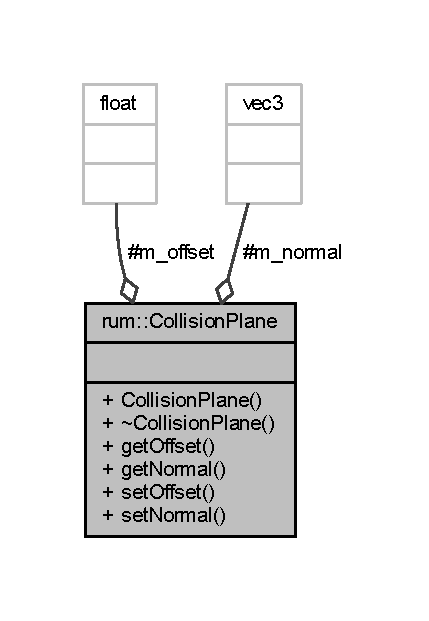
\includegraphics[width=206pt]{classrum_1_1_collision_plane__coll__graph}
\end{center}
\end{figure}
\subsection*{Public Member Functions}
\begin{DoxyCompactItemize}
\item 
\mbox{\hyperlink{classrum_1_1_collision_plane_acb1374bc8962e6f0e14a93c041ade93f}{Collision\+Plane}} (const glm\+::vec3 \&normal, \mbox{\hyperlink{namespacerum_a7e8cca23573d5eaead0f138cbaa4862c}{real}} offset)
\item 
\mbox{\hyperlink{classrum_1_1_collision_plane_aed3fc45bbe236d0e3674745ed511ea14}{$\sim$\+Collision\+Plane}} ()
\item 
\mbox{\hyperlink{namespacerum_a7e8cca23573d5eaead0f138cbaa4862c}{real}} \mbox{\hyperlink{classrum_1_1_collision_plane_a348709c5d226023ce51d17a0fdfbe408}{get\+Offset}} () const
\item 
glm\+::vec3 \mbox{\hyperlink{classrum_1_1_collision_plane_a699fae9d74e6e19c4e30870d538c3a71}{get\+Normal}} () const
\item 
void \mbox{\hyperlink{classrum_1_1_collision_plane_aeaa1d14df4d33c30a7495e72ff5fa454}{set\+Offset}} (\mbox{\hyperlink{namespacerum_a7e8cca23573d5eaead0f138cbaa4862c}{real}} offset)
\item 
void \mbox{\hyperlink{classrum_1_1_collision_plane_ade1d578943c87eba3f49134f6e19148d}{set\+Normal}} (const glm\+::vec3 \&normal)
\end{DoxyCompactItemize}
\subsection*{Protected Attributes}
\begin{DoxyCompactItemize}
\item 
glm\+::vec3 \mbox{\hyperlink{classrum_1_1_collision_plane_aa2f3d73f116cb6965cd561f25ea4b67e}{m\+\_\+normal}}
\item 
\mbox{\hyperlink{namespacerum_a7e8cca23573d5eaead0f138cbaa4862c}{real}} \mbox{\hyperlink{classrum_1_1_collision_plane_a0630544f46ad1830d7f73f94746f1f25}{m\+\_\+offset}}
\end{DoxyCompactItemize}


\subsection{Constructor \& Destructor Documentation}
\mbox{\Hypertarget{classrum_1_1_collision_plane_acb1374bc8962e6f0e14a93c041ade93f}\label{classrum_1_1_collision_plane_acb1374bc8962e6f0e14a93c041ade93f}} 
\index{rum\+::\+Collision\+Plane@{rum\+::\+Collision\+Plane}!Collision\+Plane@{Collision\+Plane}}
\index{Collision\+Plane@{Collision\+Plane}!rum\+::\+Collision\+Plane@{rum\+::\+Collision\+Plane}}
\subsubsection{\texorpdfstring{Collision\+Plane()}{CollisionPlane()}}
{\footnotesize\ttfamily rum\+::\+Collision\+Plane\+::\+Collision\+Plane (\begin{DoxyParamCaption}\item[{const glm\+::vec3 \&}]{normal,  }\item[{\mbox{\hyperlink{namespacerum_a7e8cca23573d5eaead0f138cbaa4862c}{real}}}]{offset }\end{DoxyParamCaption})}

\mbox{\Hypertarget{classrum_1_1_collision_plane_aed3fc45bbe236d0e3674745ed511ea14}\label{classrum_1_1_collision_plane_aed3fc45bbe236d0e3674745ed511ea14}} 
\index{rum\+::\+Collision\+Plane@{rum\+::\+Collision\+Plane}!````~Collision\+Plane@{$\sim$\+Collision\+Plane}}
\index{````~Collision\+Plane@{$\sim$\+Collision\+Plane}!rum\+::\+Collision\+Plane@{rum\+::\+Collision\+Plane}}
\subsubsection{\texorpdfstring{$\sim$\+Collision\+Plane()}{~CollisionPlane()}}
{\footnotesize\ttfamily rum\+::\+Collision\+Plane\+::$\sim$\+Collision\+Plane (\begin{DoxyParamCaption}{ }\end{DoxyParamCaption})\hspace{0.3cm}{\ttfamily [default]}}



\subsection{Member Function Documentation}
\mbox{\Hypertarget{classrum_1_1_collision_plane_a699fae9d74e6e19c4e30870d538c3a71}\label{classrum_1_1_collision_plane_a699fae9d74e6e19c4e30870d538c3a71}} 
\index{rum\+::\+Collision\+Plane@{rum\+::\+Collision\+Plane}!get\+Normal@{get\+Normal}}
\index{get\+Normal@{get\+Normal}!rum\+::\+Collision\+Plane@{rum\+::\+Collision\+Plane}}
\subsubsection{\texorpdfstring{get\+Normal()}{getNormal()}}
{\footnotesize\ttfamily glm\+::vec3 rum\+::\+Collision\+Plane\+::get\+Normal (\begin{DoxyParamCaption}{ }\end{DoxyParamCaption}) const}

\mbox{\Hypertarget{classrum_1_1_collision_plane_a348709c5d226023ce51d17a0fdfbe408}\label{classrum_1_1_collision_plane_a348709c5d226023ce51d17a0fdfbe408}} 
\index{rum\+::\+Collision\+Plane@{rum\+::\+Collision\+Plane}!get\+Offset@{get\+Offset}}
\index{get\+Offset@{get\+Offset}!rum\+::\+Collision\+Plane@{rum\+::\+Collision\+Plane}}
\subsubsection{\texorpdfstring{get\+Offset()}{getOffset()}}
{\footnotesize\ttfamily \mbox{\hyperlink{namespacerum_a7e8cca23573d5eaead0f138cbaa4862c}{real}} rum\+::\+Collision\+Plane\+::get\+Offset (\begin{DoxyParamCaption}{ }\end{DoxyParamCaption}) const}

\mbox{\Hypertarget{classrum_1_1_collision_plane_ade1d578943c87eba3f49134f6e19148d}\label{classrum_1_1_collision_plane_ade1d578943c87eba3f49134f6e19148d}} 
\index{rum\+::\+Collision\+Plane@{rum\+::\+Collision\+Plane}!set\+Normal@{set\+Normal}}
\index{set\+Normal@{set\+Normal}!rum\+::\+Collision\+Plane@{rum\+::\+Collision\+Plane}}
\subsubsection{\texorpdfstring{set\+Normal()}{setNormal()}}
{\footnotesize\ttfamily void rum\+::\+Collision\+Plane\+::set\+Normal (\begin{DoxyParamCaption}\item[{const glm\+::vec3 \&}]{normal }\end{DoxyParamCaption})}

\mbox{\Hypertarget{classrum_1_1_collision_plane_aeaa1d14df4d33c30a7495e72ff5fa454}\label{classrum_1_1_collision_plane_aeaa1d14df4d33c30a7495e72ff5fa454}} 
\index{rum\+::\+Collision\+Plane@{rum\+::\+Collision\+Plane}!set\+Offset@{set\+Offset}}
\index{set\+Offset@{set\+Offset}!rum\+::\+Collision\+Plane@{rum\+::\+Collision\+Plane}}
\subsubsection{\texorpdfstring{set\+Offset()}{setOffset()}}
{\footnotesize\ttfamily void rum\+::\+Collision\+Plane\+::set\+Offset (\begin{DoxyParamCaption}\item[{\mbox{\hyperlink{namespacerum_a7e8cca23573d5eaead0f138cbaa4862c}{real}}}]{offset }\end{DoxyParamCaption})}



\subsection{Member Data Documentation}
\mbox{\Hypertarget{classrum_1_1_collision_plane_aa2f3d73f116cb6965cd561f25ea4b67e}\label{classrum_1_1_collision_plane_aa2f3d73f116cb6965cd561f25ea4b67e}} 
\index{rum\+::\+Collision\+Plane@{rum\+::\+Collision\+Plane}!m\+\_\+normal@{m\+\_\+normal}}
\index{m\+\_\+normal@{m\+\_\+normal}!rum\+::\+Collision\+Plane@{rum\+::\+Collision\+Plane}}
\subsubsection{\texorpdfstring{m\+\_\+normal}{m\_normal}}
{\footnotesize\ttfamily glm\+::vec3 rum\+::\+Collision\+Plane\+::m\+\_\+normal\hspace{0.3cm}{\ttfamily [protected]}}

\mbox{\Hypertarget{classrum_1_1_collision_plane_a0630544f46ad1830d7f73f94746f1f25}\label{classrum_1_1_collision_plane_a0630544f46ad1830d7f73f94746f1f25}} 
\index{rum\+::\+Collision\+Plane@{rum\+::\+Collision\+Plane}!m\+\_\+offset@{m\+\_\+offset}}
\index{m\+\_\+offset@{m\+\_\+offset}!rum\+::\+Collision\+Plane@{rum\+::\+Collision\+Plane}}
\subsubsection{\texorpdfstring{m\+\_\+offset}{m\_offset}}
{\footnotesize\ttfamily \mbox{\hyperlink{namespacerum_a7e8cca23573d5eaead0f138cbaa4862c}{real}} rum\+::\+Collision\+Plane\+::m\+\_\+offset\hspace{0.3cm}{\ttfamily [protected]}}



The documentation for this class was generated from the following files\+:\begin{DoxyCompactItemize}
\item 
D\+:/\+Library/\+Documents/\+Job/\+Forschungsmaster/\+Projekte/\+Rumble3\+D/\+Rumble3\+D/include/\+R3\+D/\+Rigid\+Body\+Engine/\mbox{\hyperlink{_collision_plane_8h}{Collision\+Plane.\+h}}\item 
D\+:/\+Library/\+Documents/\+Job/\+Forschungsmaster/\+Projekte/\+Rumble3\+D/\+Rumble3\+D/src/\+Rigid\+Body\+Engine/\mbox{\hyperlink{_collision_plane_8cpp}{Collision\+Plane.\+cpp}}\end{DoxyCompactItemize}

\hypertarget{classrum_1_1_collision_primitive}{}\section{rum\+:\+:Collision\+Primitive Class Reference}
\label{classrum_1_1_collision_primitive}\index{rum\+::\+Collision\+Primitive@{rum\+::\+Collision\+Primitive}}


{\ttfamily \#include $<$Collision\+Primitive.\+h$>$}



Inheritance diagram for rum\+:\+:Collision\+Primitive\+:\nopagebreak
\begin{figure}[H]
\begin{center}
\leavevmode
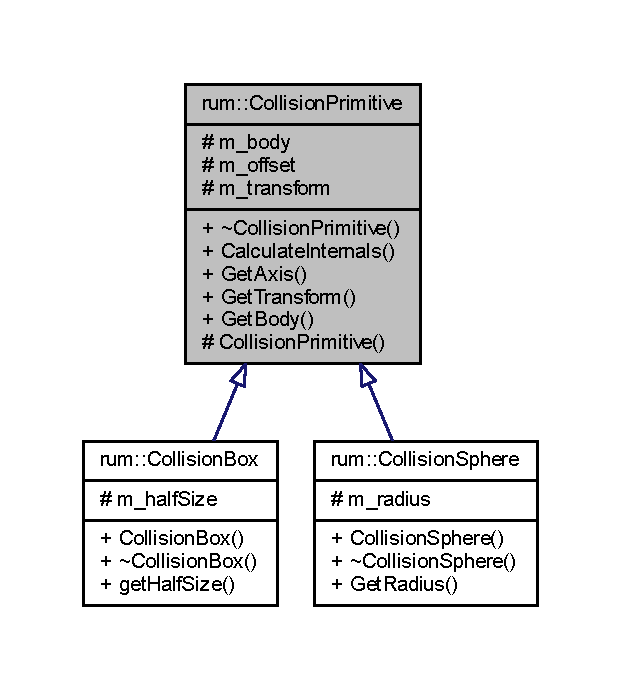
\includegraphics[width=308pt]{classrum_1_1_collision_primitive__inherit__graph}
\end{center}
\end{figure}


Collaboration diagram for rum\+:\+:Collision\+Primitive\+:\nopagebreak
\begin{figure}[H]
\begin{center}
\leavevmode
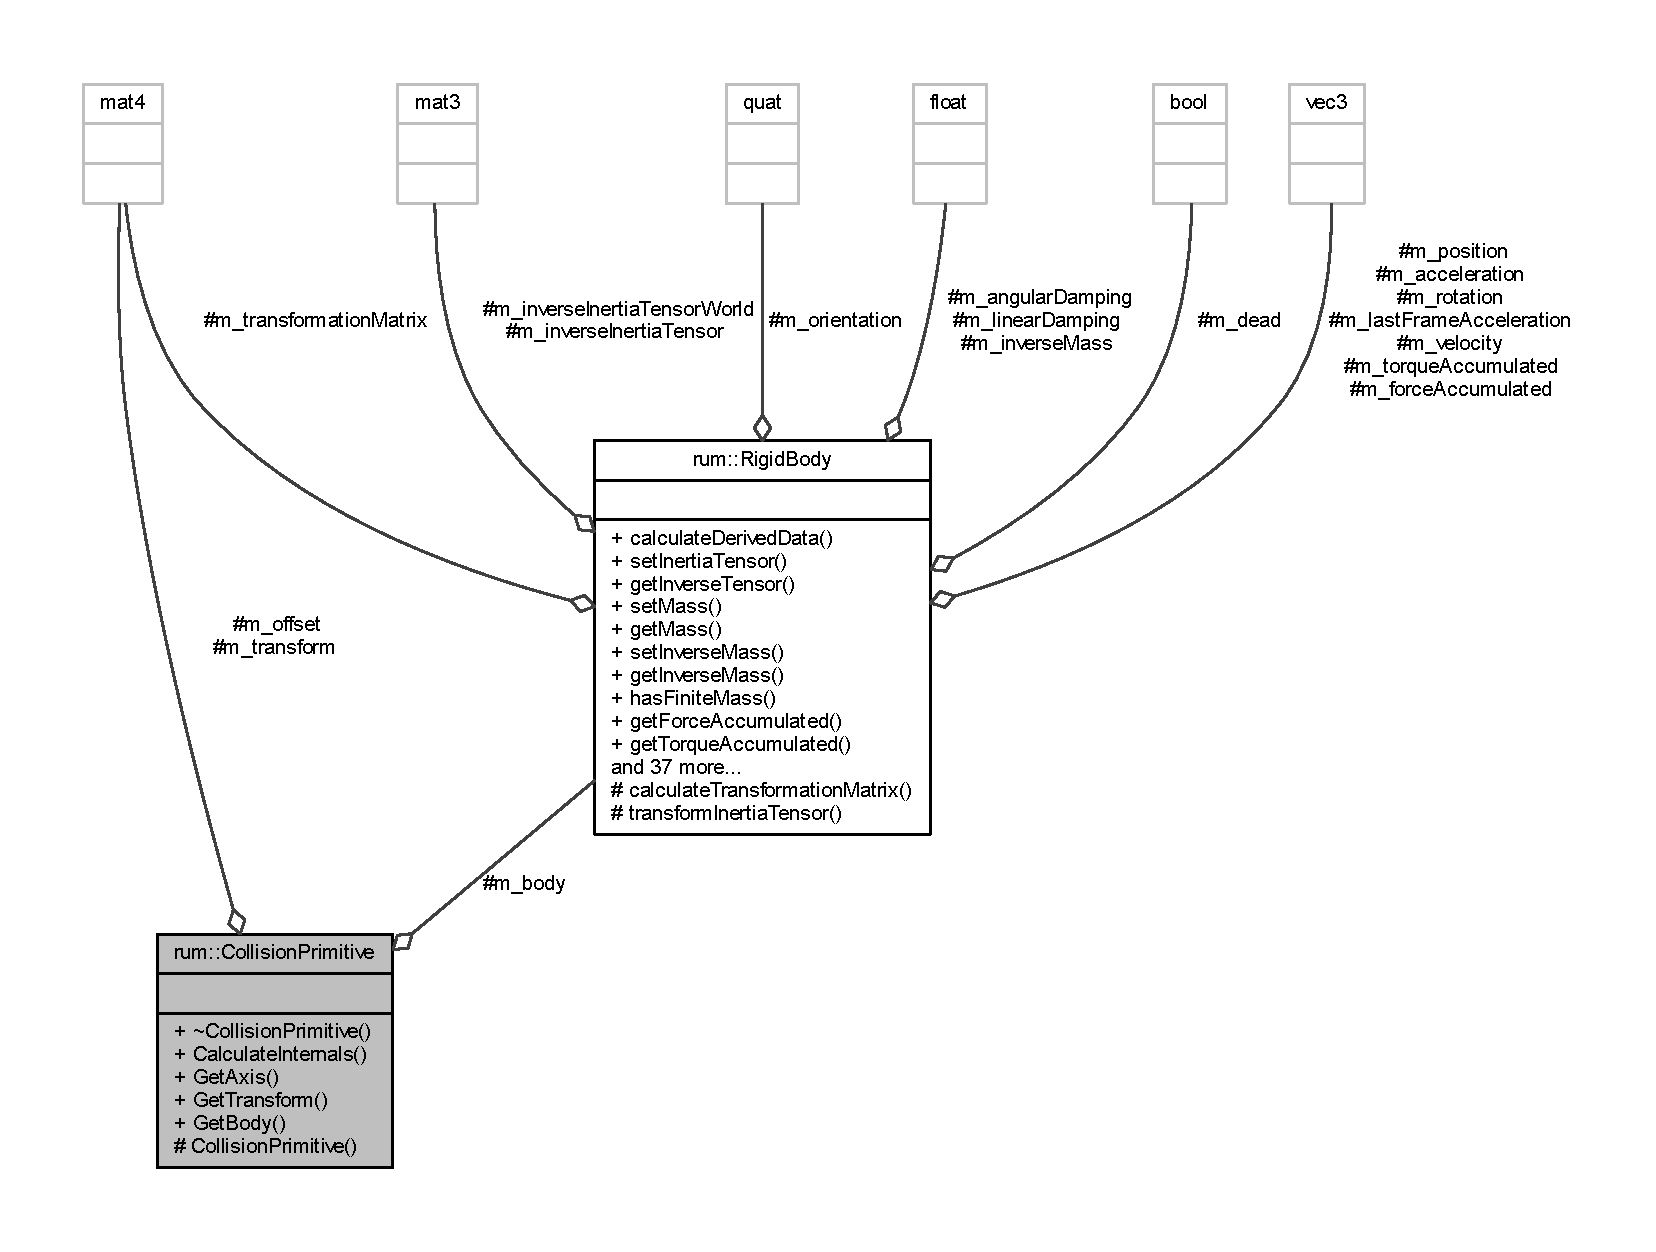
\includegraphics[width=350pt]{classrum_1_1_collision_primitive__coll__graph}
\end{center}
\end{figure}
\subsection*{Public Member Functions}
\begin{DoxyCompactItemize}
\item 
virtual \mbox{\hyperlink{classrum_1_1_collision_primitive_aaaa286303df8a1af561d698b4bb9f098}{$\sim$\+Collision\+Primitive}} ()
\item 
virtual void \mbox{\hyperlink{classrum_1_1_collision_primitive_a31af51e97485378954de219b8411a27d}{generate\+Contact}} (\mbox{\hyperlink{classrum_1_1_i_narrow_phase_filter}{I\+Narrow\+Phase\+Filter}} $\ast$filter, \mbox{\hyperlink{classrum_1_1_collision_primitive}{Collision\+Primitive}} $\ast$other)=0
\item 
void \mbox{\hyperlink{classrum_1_1_collision_primitive_afc7ac93a15b890539a4721638cbffe5a}{generate\+Contact}} (\mbox{\hyperlink{classrum_1_1_i_narrow_phase_filter}{I\+Narrow\+Phase\+Filter}} $\ast$filter, \mbox{\hyperlink{classrum_1_1_collision_box}{Collision\+Box}} $\ast$other)
\item 
void \mbox{\hyperlink{classrum_1_1_collision_primitive_a76af82066bef75988cce50fb3ac9e536}{generate\+Contact}} (\mbox{\hyperlink{classrum_1_1_i_narrow_phase_filter}{I\+Narrow\+Phase\+Filter}} $\ast$filter, \mbox{\hyperlink{classrum_1_1_collision_sphere}{Collision\+Sphere}} $\ast$other)
\item 
void \mbox{\hyperlink{classrum_1_1_collision_primitive_a422c1a39ca224b97e977022b5c781047}{calculate\+Internals}} ()
\item 
glm\+::vec3 \mbox{\hyperlink{classrum_1_1_collision_primitive_ad576d6ca6004b953fc7887b97856ee35}{get\+Axis}} (unsigned index) const
\item 
const glm\+::mat4 \& \mbox{\hyperlink{classrum_1_1_collision_primitive_a320a36ec6157bcdd373f40e5e9ab55d3}{get\+Transform}} () const
\item 
\mbox{\hyperlink{classrum_1_1_rigid_body}{Rigid\+Body}} $\ast$ \mbox{\hyperlink{classrum_1_1_collision_primitive_a36bb78c4a8e89c0000d91c228801e387}{get\+Body}} () const
\end{DoxyCompactItemize}
\subsection*{Protected Member Functions}
\begin{DoxyCompactItemize}
\item 
\mbox{\hyperlink{classrum_1_1_collision_primitive_af314a601d4528bc79710e9e7d9d0413e}{Collision\+Primitive}} ()
\end{DoxyCompactItemize}
\subsection*{Protected Attributes}
\begin{DoxyCompactItemize}
\item 
\mbox{\hyperlink{classrum_1_1_rigid_body}{Rigid\+Body}} $\ast$ \mbox{\hyperlink{classrum_1_1_collision_primitive_a9ef6e9862ac5e75330395368e401530e}{m\+\_\+body}} \{\}
\item 
glm\+::mat4 \mbox{\hyperlink{classrum_1_1_collision_primitive_a1617f197d7dbf54801bb21fbcedf730e}{m\+\_\+offset}}
\item 
glm\+::mat4 \mbox{\hyperlink{classrum_1_1_collision_primitive_a17dea68b6d2faa8573935fbaf4e81440}{m\+\_\+transform}}
\end{DoxyCompactItemize}


\subsection{Constructor \& Destructor Documentation}
\mbox{\Hypertarget{classrum_1_1_collision_primitive_aaaa286303df8a1af561d698b4bb9f098}\label{classrum_1_1_collision_primitive_aaaa286303df8a1af561d698b4bb9f098}} 
\index{rum\+::\+Collision\+Primitive@{rum\+::\+Collision\+Primitive}!````~Collision\+Primitive@{$\sim$\+Collision\+Primitive}}
\index{````~Collision\+Primitive@{$\sim$\+Collision\+Primitive}!rum\+::\+Collision\+Primitive@{rum\+::\+Collision\+Primitive}}
\subsubsection{\texorpdfstring{$\sim$\+Collision\+Primitive()}{~CollisionPrimitive()}}
{\footnotesize\ttfamily rum\+::\+Collision\+Primitive\+::$\sim$\+Collision\+Primitive (\begin{DoxyParamCaption}{ }\end{DoxyParamCaption})\hspace{0.3cm}{\ttfamily [virtual]}, {\ttfamily [default]}}

\mbox{\Hypertarget{classrum_1_1_collision_primitive_af314a601d4528bc79710e9e7d9d0413e}\label{classrum_1_1_collision_primitive_af314a601d4528bc79710e9e7d9d0413e}} 
\index{rum\+::\+Collision\+Primitive@{rum\+::\+Collision\+Primitive}!Collision\+Primitive@{Collision\+Primitive}}
\index{Collision\+Primitive@{Collision\+Primitive}!rum\+::\+Collision\+Primitive@{rum\+::\+Collision\+Primitive}}
\subsubsection{\texorpdfstring{Collision\+Primitive()}{CollisionPrimitive()}}
{\footnotesize\ttfamily rum\+::\+Collision\+Primitive\+::\+Collision\+Primitive (\begin{DoxyParamCaption}{ }\end{DoxyParamCaption})\hspace{0.3cm}{\ttfamily [explicit]}, {\ttfamily [protected]}, {\ttfamily [default]}}



\subsection{Member Function Documentation}
\mbox{\Hypertarget{classrum_1_1_collision_primitive_a422c1a39ca224b97e977022b5c781047}\label{classrum_1_1_collision_primitive_a422c1a39ca224b97e977022b5c781047}} 
\index{rum\+::\+Collision\+Primitive@{rum\+::\+Collision\+Primitive}!calculate\+Internals@{calculate\+Internals}}
\index{calculate\+Internals@{calculate\+Internals}!rum\+::\+Collision\+Primitive@{rum\+::\+Collision\+Primitive}}
\subsubsection{\texorpdfstring{calculate\+Internals()}{calculateInternals()}}
{\footnotesize\ttfamily void rum\+::\+Collision\+Primitive\+::calculate\+Internals (\begin{DoxyParamCaption}{ }\end{DoxyParamCaption})}

\mbox{\Hypertarget{classrum_1_1_collision_primitive_a31af51e97485378954de219b8411a27d}\label{classrum_1_1_collision_primitive_a31af51e97485378954de219b8411a27d}} 
\index{rum\+::\+Collision\+Primitive@{rum\+::\+Collision\+Primitive}!generate\+Contact@{generate\+Contact}}
\index{generate\+Contact@{generate\+Contact}!rum\+::\+Collision\+Primitive@{rum\+::\+Collision\+Primitive}}
\subsubsection{\texorpdfstring{generate\+Contact()}{generateContact()}\hspace{0.1cm}{\footnotesize\ttfamily [1/3]}}
{\footnotesize\ttfamily virtual void rum\+::\+Collision\+Primitive\+::generate\+Contact (\begin{DoxyParamCaption}\item[{\mbox{\hyperlink{classrum_1_1_i_narrow_phase_filter}{I\+Narrow\+Phase\+Filter}} $\ast$}]{filter,  }\item[{\mbox{\hyperlink{classrum_1_1_collision_primitive}{Collision\+Primitive}} $\ast$}]{other }\end{DoxyParamCaption})\hspace{0.3cm}{\ttfamily [pure virtual]}}



Implemented in \mbox{\hyperlink{classrum_1_1_collision_box_a3f72c354e24f866be640f0b3f8e2a4b4}{rum\+::\+Collision\+Box}}, and \mbox{\hyperlink{classrum_1_1_collision_sphere_a4101051ee3213ce5257adcabd1529c00}{rum\+::\+Collision\+Sphere}}.

\mbox{\Hypertarget{classrum_1_1_collision_primitive_afc7ac93a15b890539a4721638cbffe5a}\label{classrum_1_1_collision_primitive_afc7ac93a15b890539a4721638cbffe5a}} 
\index{rum\+::\+Collision\+Primitive@{rum\+::\+Collision\+Primitive}!generate\+Contact@{generate\+Contact}}
\index{generate\+Contact@{generate\+Contact}!rum\+::\+Collision\+Primitive@{rum\+::\+Collision\+Primitive}}
\subsubsection{\texorpdfstring{generate\+Contact()}{generateContact()}\hspace{0.1cm}{\footnotesize\ttfamily [2/3]}}
{\footnotesize\ttfamily void rum\+::\+Collision\+Primitive\+::generate\+Contact (\begin{DoxyParamCaption}\item[{\mbox{\hyperlink{classrum_1_1_i_narrow_phase_filter}{I\+Narrow\+Phase\+Filter}} $\ast$}]{filter,  }\item[{\mbox{\hyperlink{classrum_1_1_collision_box}{Collision\+Box}} $\ast$}]{other }\end{DoxyParamCaption})}

\mbox{\Hypertarget{classrum_1_1_collision_primitive_a76af82066bef75988cce50fb3ac9e536}\label{classrum_1_1_collision_primitive_a76af82066bef75988cce50fb3ac9e536}} 
\index{rum\+::\+Collision\+Primitive@{rum\+::\+Collision\+Primitive}!generate\+Contact@{generate\+Contact}}
\index{generate\+Contact@{generate\+Contact}!rum\+::\+Collision\+Primitive@{rum\+::\+Collision\+Primitive}}
\subsubsection{\texorpdfstring{generate\+Contact()}{generateContact()}\hspace{0.1cm}{\footnotesize\ttfamily [3/3]}}
{\footnotesize\ttfamily void rum\+::\+Collision\+Primitive\+::generate\+Contact (\begin{DoxyParamCaption}\item[{\mbox{\hyperlink{classrum_1_1_i_narrow_phase_filter}{I\+Narrow\+Phase\+Filter}} $\ast$}]{filter,  }\item[{\mbox{\hyperlink{classrum_1_1_collision_sphere}{Collision\+Sphere}} $\ast$}]{other }\end{DoxyParamCaption})}

\mbox{\Hypertarget{classrum_1_1_collision_primitive_ad576d6ca6004b953fc7887b97856ee35}\label{classrum_1_1_collision_primitive_ad576d6ca6004b953fc7887b97856ee35}} 
\index{rum\+::\+Collision\+Primitive@{rum\+::\+Collision\+Primitive}!get\+Axis@{get\+Axis}}
\index{get\+Axis@{get\+Axis}!rum\+::\+Collision\+Primitive@{rum\+::\+Collision\+Primitive}}
\subsubsection{\texorpdfstring{get\+Axis()}{getAxis()}}
{\footnotesize\ttfamily glm\+::vec3 rum\+::\+Collision\+Primitive\+::get\+Axis (\begin{DoxyParamCaption}\item[{unsigned}]{index }\end{DoxyParamCaption}) const}

\mbox{\Hypertarget{classrum_1_1_collision_primitive_a36bb78c4a8e89c0000d91c228801e387}\label{classrum_1_1_collision_primitive_a36bb78c4a8e89c0000d91c228801e387}} 
\index{rum\+::\+Collision\+Primitive@{rum\+::\+Collision\+Primitive}!get\+Body@{get\+Body}}
\index{get\+Body@{get\+Body}!rum\+::\+Collision\+Primitive@{rum\+::\+Collision\+Primitive}}
\subsubsection{\texorpdfstring{get\+Body()}{getBody()}}
{\footnotesize\ttfamily \mbox{\hyperlink{classrum_1_1_rigid_body}{Rigid\+Body}} $\ast$ rum\+::\+Collision\+Primitive\+::get\+Body (\begin{DoxyParamCaption}{ }\end{DoxyParamCaption}) const}

\mbox{\Hypertarget{classrum_1_1_collision_primitive_a320a36ec6157bcdd373f40e5e9ab55d3}\label{classrum_1_1_collision_primitive_a320a36ec6157bcdd373f40e5e9ab55d3}} 
\index{rum\+::\+Collision\+Primitive@{rum\+::\+Collision\+Primitive}!get\+Transform@{get\+Transform}}
\index{get\+Transform@{get\+Transform}!rum\+::\+Collision\+Primitive@{rum\+::\+Collision\+Primitive}}
\subsubsection{\texorpdfstring{get\+Transform()}{getTransform()}}
{\footnotesize\ttfamily const glm\+::mat4 \& rum\+::\+Collision\+Primitive\+::get\+Transform (\begin{DoxyParamCaption}{ }\end{DoxyParamCaption}) const}



\subsection{Member Data Documentation}
\mbox{\Hypertarget{classrum_1_1_collision_primitive_a9ef6e9862ac5e75330395368e401530e}\label{classrum_1_1_collision_primitive_a9ef6e9862ac5e75330395368e401530e}} 
\index{rum\+::\+Collision\+Primitive@{rum\+::\+Collision\+Primitive}!m\+\_\+body@{m\+\_\+body}}
\index{m\+\_\+body@{m\+\_\+body}!rum\+::\+Collision\+Primitive@{rum\+::\+Collision\+Primitive}}
\subsubsection{\texorpdfstring{m\+\_\+body}{m\_body}}
{\footnotesize\ttfamily \mbox{\hyperlink{classrum_1_1_rigid_body}{Rigid\+Body}}$\ast$ rum\+::\+Collision\+Primitive\+::m\+\_\+body \{\}\hspace{0.3cm}{\ttfamily [protected]}}

\mbox{\Hypertarget{classrum_1_1_collision_primitive_a1617f197d7dbf54801bb21fbcedf730e}\label{classrum_1_1_collision_primitive_a1617f197d7dbf54801bb21fbcedf730e}} 
\index{rum\+::\+Collision\+Primitive@{rum\+::\+Collision\+Primitive}!m\+\_\+offset@{m\+\_\+offset}}
\index{m\+\_\+offset@{m\+\_\+offset}!rum\+::\+Collision\+Primitive@{rum\+::\+Collision\+Primitive}}
\subsubsection{\texorpdfstring{m\+\_\+offset}{m\_offset}}
{\footnotesize\ttfamily glm\+::mat4 rum\+::\+Collision\+Primitive\+::m\+\_\+offset\hspace{0.3cm}{\ttfamily [protected]}}

\mbox{\Hypertarget{classrum_1_1_collision_primitive_a17dea68b6d2faa8573935fbaf4e81440}\label{classrum_1_1_collision_primitive_a17dea68b6d2faa8573935fbaf4e81440}} 
\index{rum\+::\+Collision\+Primitive@{rum\+::\+Collision\+Primitive}!m\+\_\+transform@{m\+\_\+transform}}
\index{m\+\_\+transform@{m\+\_\+transform}!rum\+::\+Collision\+Primitive@{rum\+::\+Collision\+Primitive}}
\subsubsection{\texorpdfstring{m\+\_\+transform}{m\_transform}}
{\footnotesize\ttfamily glm\+::mat4 rum\+::\+Collision\+Primitive\+::m\+\_\+transform\hspace{0.3cm}{\ttfamily [protected]}}



The documentation for this class was generated from the following files\+:\begin{DoxyCompactItemize}
\item 
D\+:/\+Library/\+Documents/\+Job/\+Forschungsmaster/\+Projekte/\+Rumble3\+D/\+Rumble3\+D/include/\+R3\+D/\+Rigid\+Body\+Engine/\mbox{\hyperlink{_collision_primitive_8h}{Collision\+Primitive.\+h}}\item 
D\+:/\+Library/\+Documents/\+Job/\+Forschungsmaster/\+Projekte/\+Rumble3\+D/\+Rumble3\+D/src/\+Rigid\+Body\+Engine/\mbox{\hyperlink{_collision_primitive_8cpp}{Collision\+Primitive.\+cpp}}\end{DoxyCompactItemize}

\hypertarget{classrum_1_1_collision_sphere}{}\section{rum\+:\+:Collision\+Sphere Class Reference}
\label{classrum_1_1_collision_sphere}\index{rum\+::\+Collision\+Sphere@{rum\+::\+Collision\+Sphere}}


{\ttfamily \#include $<$Collision\+Sphere.\+h$>$}



Inheritance diagram for rum\+:\+:Collision\+Sphere\+:\nopagebreak
\begin{figure}[H]
\begin{center}
\leavevmode
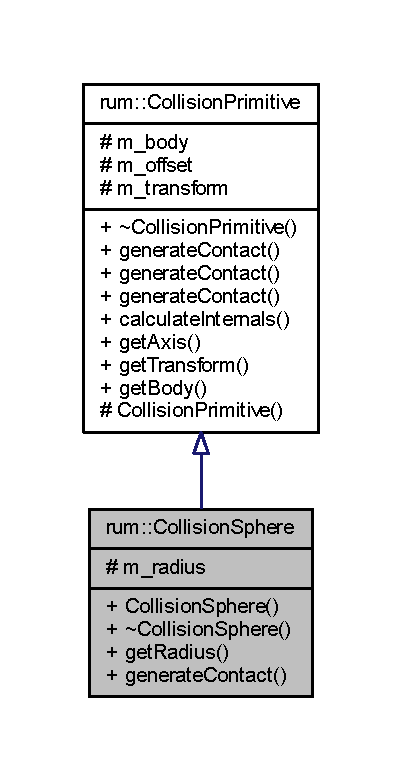
\includegraphics[width=193pt]{classrum_1_1_collision_sphere__inherit__graph}
\end{center}
\end{figure}


Collaboration diagram for rum\+:\+:Collision\+Sphere\+:\nopagebreak
\begin{figure}[H]
\begin{center}
\leavevmode
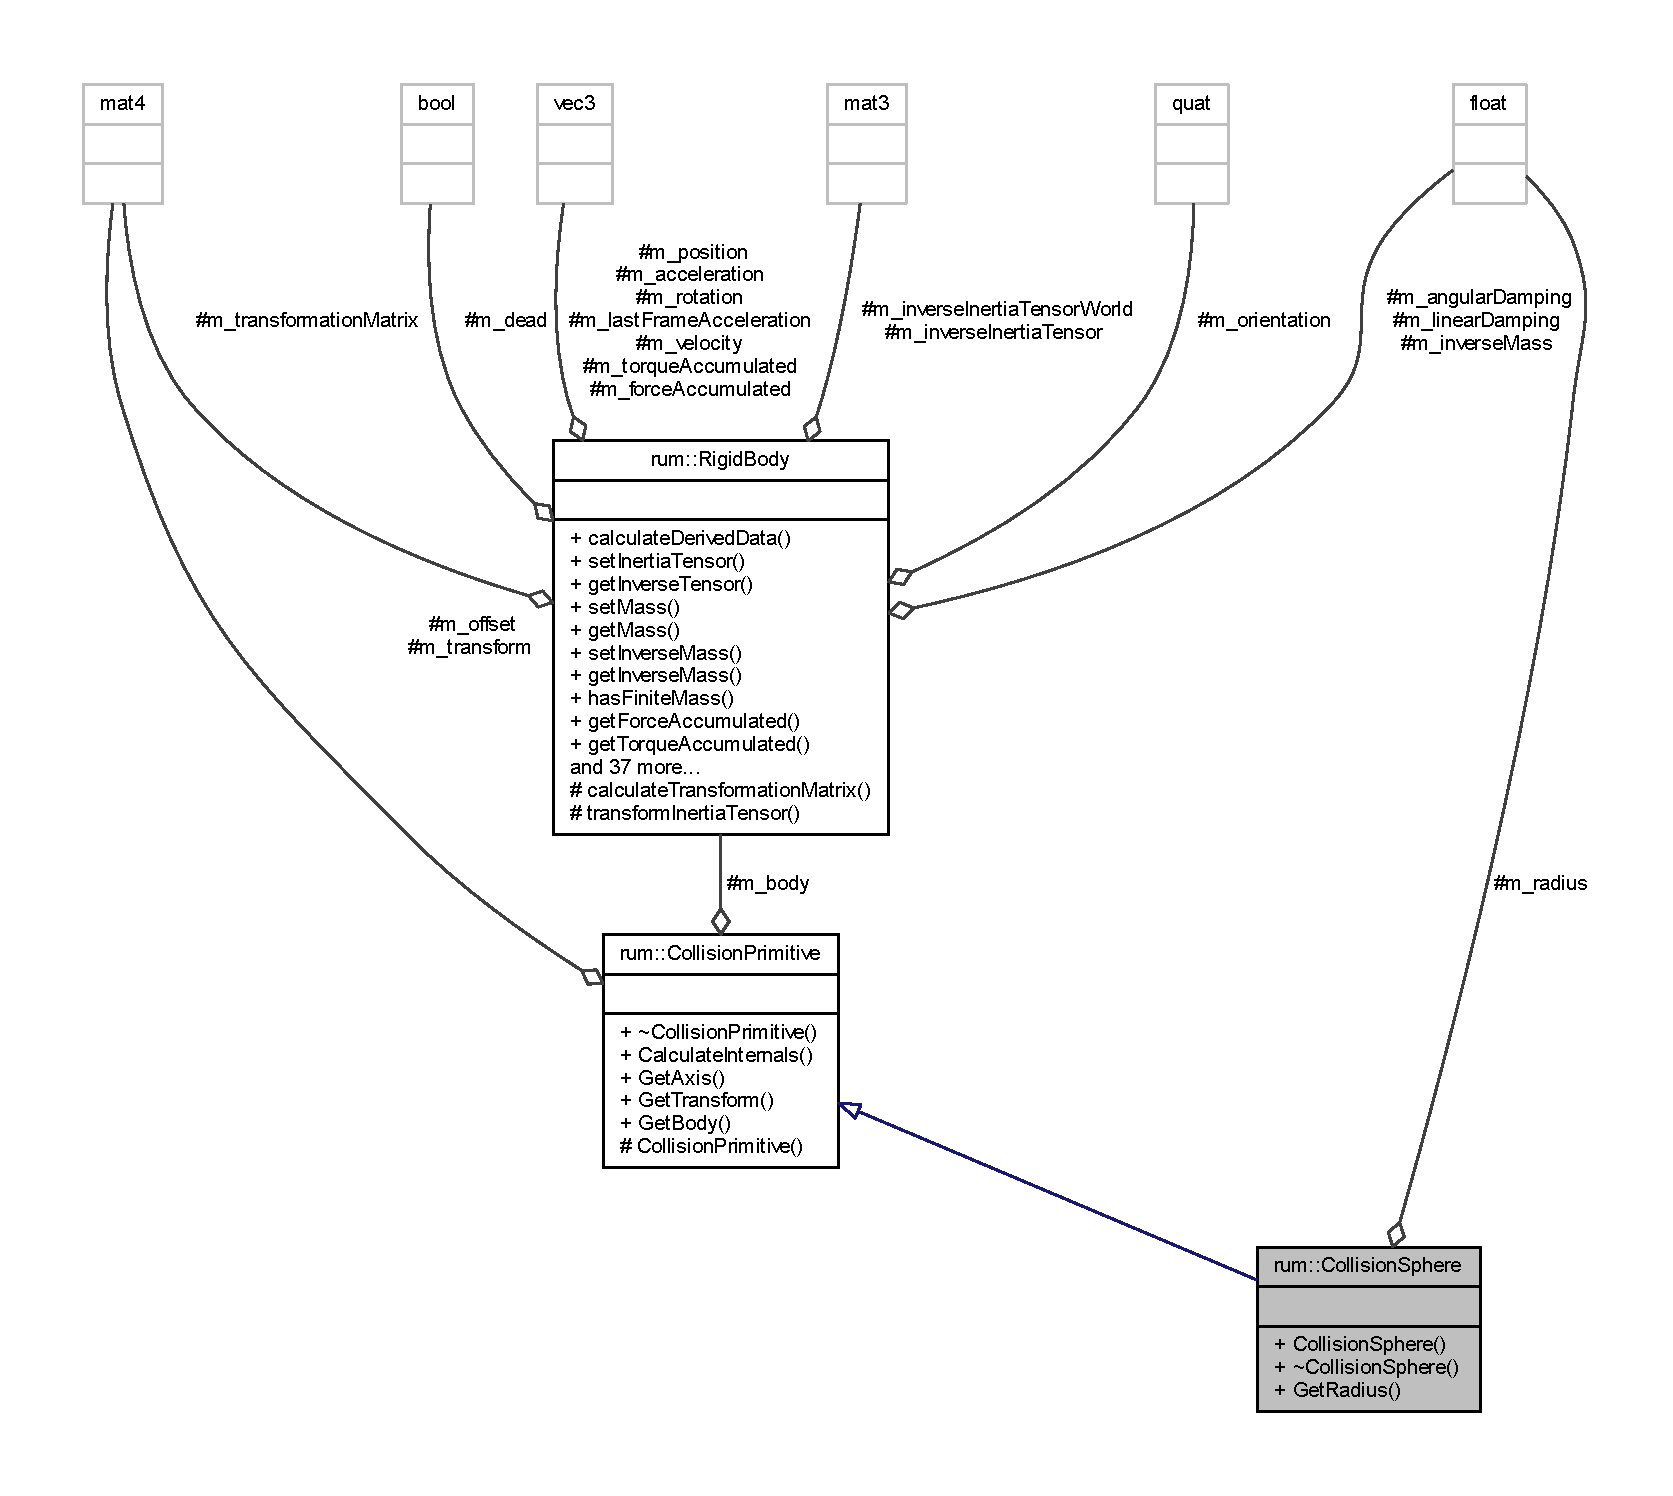
\includegraphics[width=350pt]{classrum_1_1_collision_sphere__coll__graph}
\end{center}
\end{figure}
\subsection*{Public Member Functions}
\begin{DoxyCompactItemize}
\item 
\hyperlink{classrum_1_1_collision_sphere_abdd9300c4f88d40d1b131cfcae6b94df}{Collision\+Sphere} (\hyperlink{classrum_1_1_rigid_body}{Rigid\+Body} $\ast$body, glm\+::mat4 offset, \hyperlink{namespacerum_a7e8cca23573d5eaead0f138cbaa4862c}{real} radius)
\item 
\hyperlink{classrum_1_1_collision_sphere_a6e3be5263f114a38ecb3bbf9b97ba8df}{$\sim$\+Collision\+Sphere} ()
\item 
\hyperlink{namespacerum_a7e8cca23573d5eaead0f138cbaa4862c}{real} \hyperlink{classrum_1_1_collision_sphere_a766fafc15150c2b14f2545c2401f35e1}{Get\+Radius} () const
\end{DoxyCompactItemize}
\subsection*{Protected Attributes}
\begin{DoxyCompactItemize}
\item 
\hyperlink{namespacerum_a7e8cca23573d5eaead0f138cbaa4862c}{real} \hyperlink{classrum_1_1_collision_sphere_a191922b8ffb7ea87aa1caf915c563aad}{m\+\_\+radius}
\end{DoxyCompactItemize}
\subsection*{Additional Inherited Members}


\subsection{Constructor \& Destructor Documentation}
\mbox{\Hypertarget{classrum_1_1_collision_sphere_abdd9300c4f88d40d1b131cfcae6b94df}\label{classrum_1_1_collision_sphere_abdd9300c4f88d40d1b131cfcae6b94df}} 
\index{rum\+::\+Collision\+Sphere@{rum\+::\+Collision\+Sphere}!Collision\+Sphere@{Collision\+Sphere}}
\index{Collision\+Sphere@{Collision\+Sphere}!rum\+::\+Collision\+Sphere@{rum\+::\+Collision\+Sphere}}
\subsubsection{\texorpdfstring{Collision\+Sphere()}{CollisionSphere()}}
{\footnotesize\ttfamily rum\+::\+Collision\+Sphere\+::\+Collision\+Sphere (\begin{DoxyParamCaption}\item[{\hyperlink{classrum_1_1_rigid_body}{Rigid\+Body} $\ast$}]{body,  }\item[{glm\+::mat4}]{offset,  }\item[{\hyperlink{namespacerum_a7e8cca23573d5eaead0f138cbaa4862c}{real}}]{radius }\end{DoxyParamCaption})}

\mbox{\Hypertarget{classrum_1_1_collision_sphere_a6e3be5263f114a38ecb3bbf9b97ba8df}\label{classrum_1_1_collision_sphere_a6e3be5263f114a38ecb3bbf9b97ba8df}} 
\index{rum\+::\+Collision\+Sphere@{rum\+::\+Collision\+Sphere}!````~Collision\+Sphere@{$\sim$\+Collision\+Sphere}}
\index{````~Collision\+Sphere@{$\sim$\+Collision\+Sphere}!rum\+::\+Collision\+Sphere@{rum\+::\+Collision\+Sphere}}
\subsubsection{\texorpdfstring{$\sim$\+Collision\+Sphere()}{~CollisionSphere()}}
{\footnotesize\ttfamily rum\+::\+Collision\+Sphere\+::$\sim$\+Collision\+Sphere (\begin{DoxyParamCaption}{ }\end{DoxyParamCaption})}



\subsection{Member Function Documentation}
\mbox{\Hypertarget{classrum_1_1_collision_sphere_a766fafc15150c2b14f2545c2401f35e1}\label{classrum_1_1_collision_sphere_a766fafc15150c2b14f2545c2401f35e1}} 
\index{rum\+::\+Collision\+Sphere@{rum\+::\+Collision\+Sphere}!Get\+Radius@{Get\+Radius}}
\index{Get\+Radius@{Get\+Radius}!rum\+::\+Collision\+Sphere@{rum\+::\+Collision\+Sphere}}
\subsubsection{\texorpdfstring{Get\+Radius()}{GetRadius()}}
{\footnotesize\ttfamily \hyperlink{namespacerum_a7e8cca23573d5eaead0f138cbaa4862c}{real} rum\+::\+Collision\+Sphere\+::\+Get\+Radius (\begin{DoxyParamCaption}{ }\end{DoxyParamCaption}) const}



\subsection{Member Data Documentation}
\mbox{\Hypertarget{classrum_1_1_collision_sphere_a191922b8ffb7ea87aa1caf915c563aad}\label{classrum_1_1_collision_sphere_a191922b8ffb7ea87aa1caf915c563aad}} 
\index{rum\+::\+Collision\+Sphere@{rum\+::\+Collision\+Sphere}!m\+\_\+radius@{m\+\_\+radius}}
\index{m\+\_\+radius@{m\+\_\+radius}!rum\+::\+Collision\+Sphere@{rum\+::\+Collision\+Sphere}}
\subsubsection{\texorpdfstring{m\+\_\+radius}{m\_radius}}
{\footnotesize\ttfamily \hyperlink{namespacerum_a7e8cca23573d5eaead0f138cbaa4862c}{real} rum\+::\+Collision\+Sphere\+::m\+\_\+radius\hspace{0.3cm}{\ttfamily [protected]}}



The documentation for this class was generated from the following files\+:\begin{DoxyCompactItemize}
\item 
F\+:/\+Library/\+Documents/\+Job/\+Forschungsmaster/\+Rumble3\+D/\+Rumble3\+D/include/\+R3\+D/\+Rigid\+Body\+Engine/\hyperlink{_collision_sphere_8h}{Collision\+Sphere.\+h}\item 
F\+:/\+Library/\+Documents/\+Job/\+Forschungsmaster/\+Rumble3\+D/\+Rumble3\+D/src/\+Rigid\+Body\+Engine/\hyperlink{_collision_sphere_8cpp}{Collision\+Sphere.\+cpp}\end{DoxyCompactItemize}

\hypertarget{classrum_1_1_contact}{}\section{rum\+:\+:Contact Class Reference}
\label{classrum_1_1_contact}\index{rum\+::\+Contact@{rum\+::\+Contact}}


{\ttfamily \#include $<$Contact.\+h$>$}



Collaboration diagram for rum\+:\+:Contact\+:\nopagebreak
\begin{figure}[H]
\begin{center}
\leavevmode
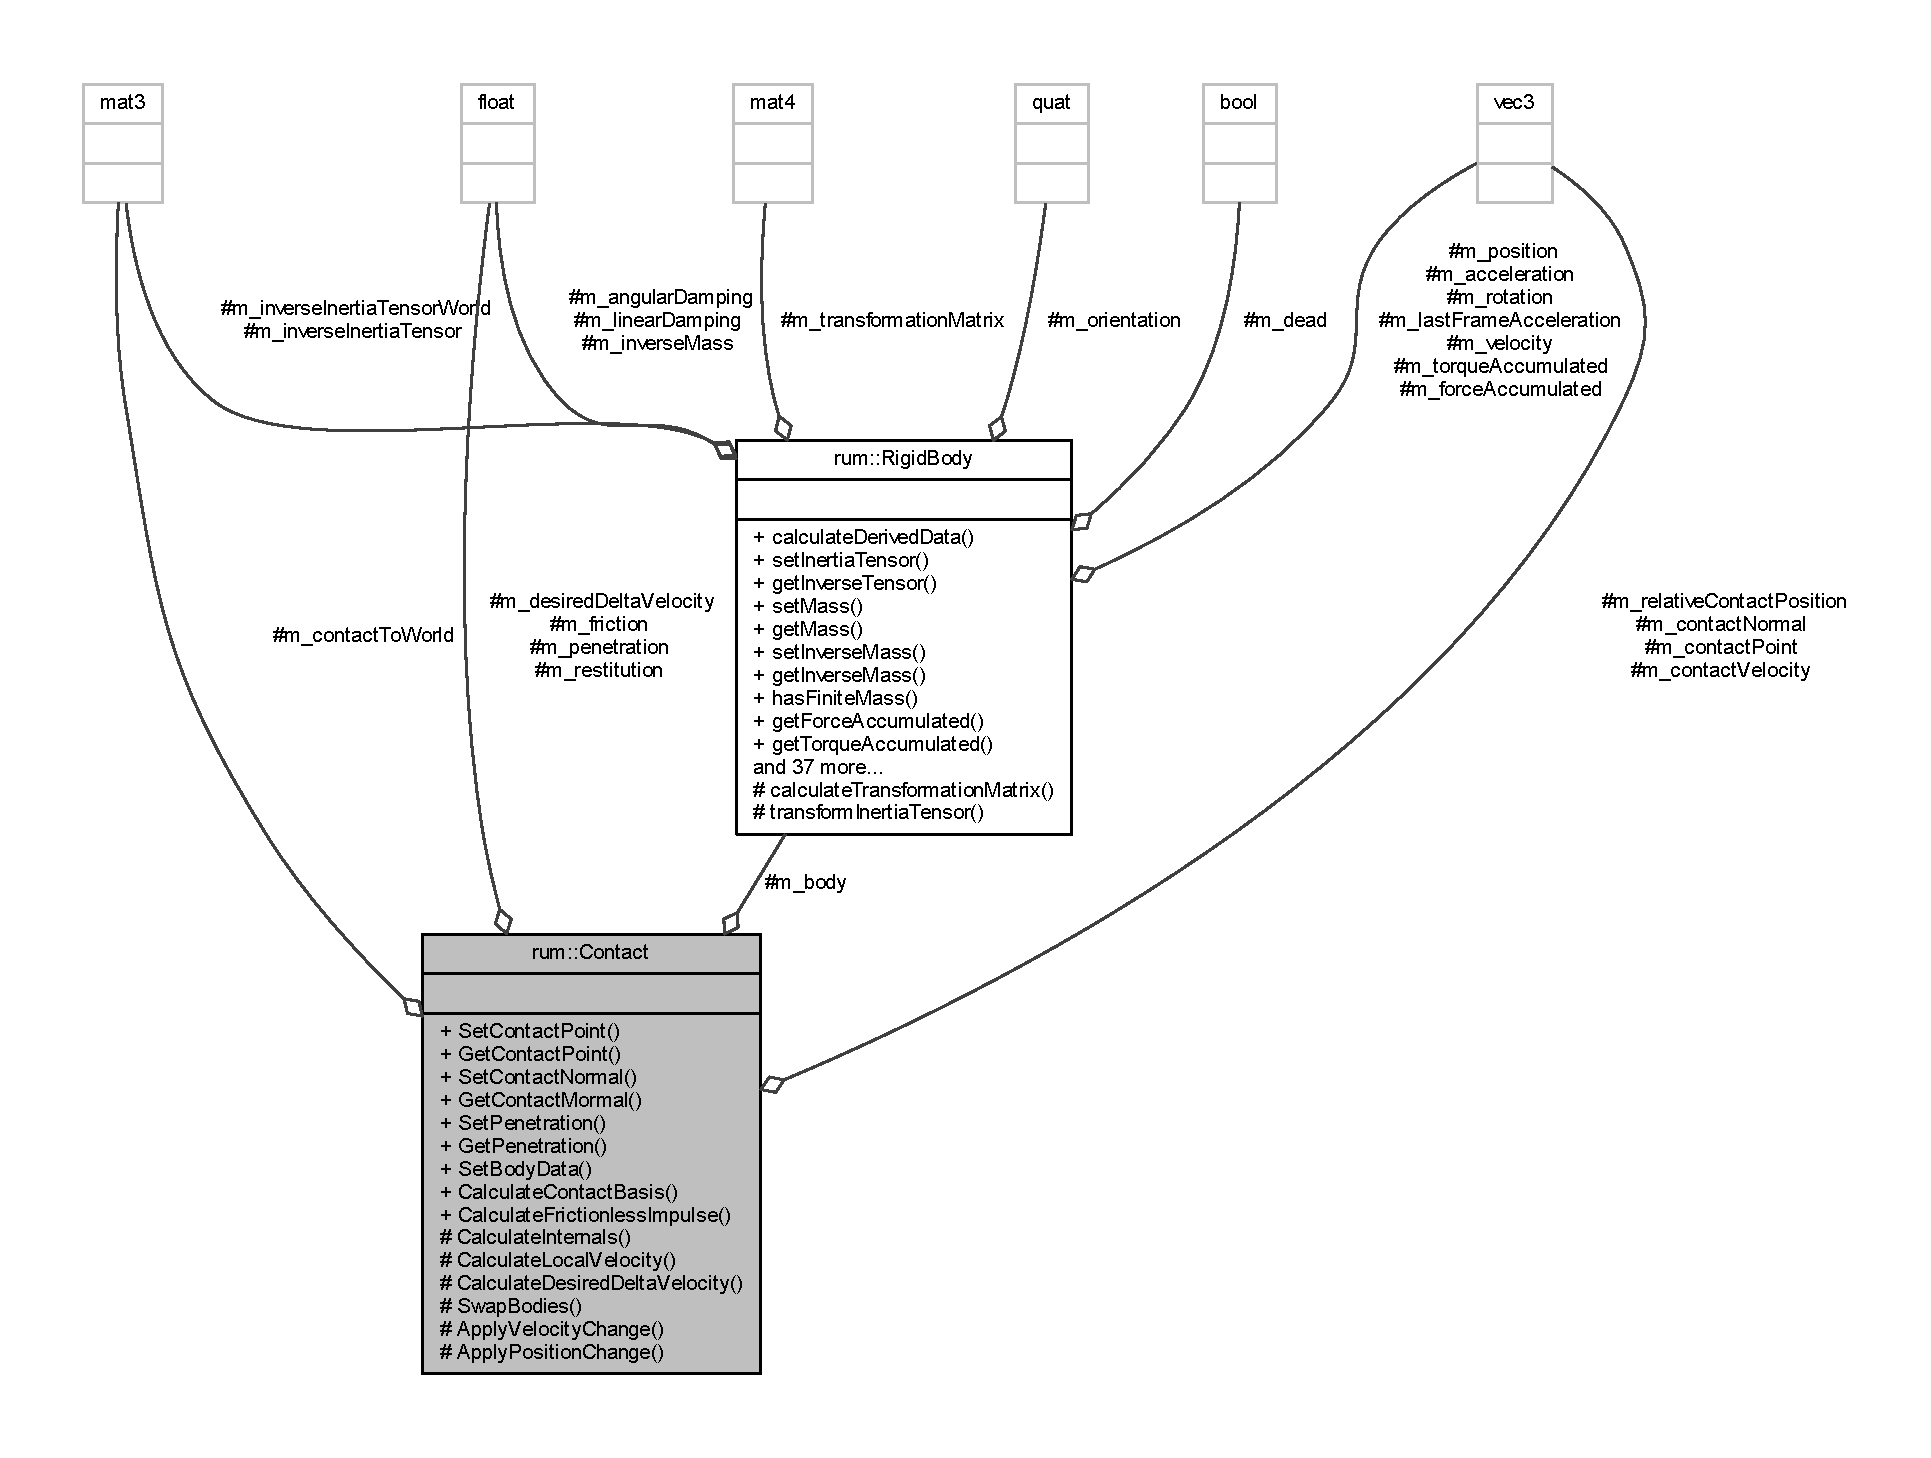
\includegraphics[width=350pt]{classrum_1_1_contact__coll__graph}
\end{center}
\end{figure}
\subsection*{Public Member Functions}
\begin{DoxyCompactItemize}
\item 
void \hyperlink{classrum_1_1_contact_a64ba0fca39f090fd7f211cb1a7585578}{Set\+Contact\+Point} (const glm\+::vec3 \&contact\+Point)
\item 
glm\+::vec3 \hyperlink{classrum_1_1_contact_a1a21b5351b7b4a84e05557232cc8b838}{Get\+Contact\+Point} ()
\item 
void \hyperlink{classrum_1_1_contact_a0e0cd538aab86185bd22e6660e225db2}{Set\+Contact\+Normal} (const glm\+::vec3 \&contact\+Normal)
\item 
glm\+::vec3 \hyperlink{classrum_1_1_contact_a4f3310ec7a77f61dbf8733b0fe127550}{Get\+Contact\+Mormal} ()
\item 
void \hyperlink{classrum_1_1_contact_a713b7b8eb8adcf50a616ab9e1b391ecc}{Set\+Penetration} (const \hyperlink{namespacerum_a7e8cca23573d5eaead0f138cbaa4862c}{real} penetration)
\item 
\hyperlink{namespacerum_a7e8cca23573d5eaead0f138cbaa4862c}{real} \hyperlink{classrum_1_1_contact_a337aa264d344357959c3f31494610292}{Get\+Penetration} ()
\item 
void \hyperlink{classrum_1_1_contact_ada3b091bf846f790e889c9cc526f47df}{Set\+Body\+Data} (\hyperlink{classrum_1_1_rigid_body}{Rigid\+Body} $\ast$one, \hyperlink{classrum_1_1_rigid_body}{Rigid\+Body} $\ast$two, \hyperlink{namespacerum_a7e8cca23573d5eaead0f138cbaa4862c}{real} friction, \hyperlink{namespacerum_a7e8cca23573d5eaead0f138cbaa4862c}{real} restitution)
\item 
void \hyperlink{classrum_1_1_contact_af2b19ba7393d8596ec34aac2de9aebfa}{Calculate\+Contact\+Basis} ()
\item 
glm\+::vec3 \hyperlink{classrum_1_1_contact_a74dad6b365bbe5337e61c2cfeed9f247}{Calculate\+Frictionless\+Impulse} (glm\+::mat3 $\ast$inverse\+Inertia\+Tensor)
\end{DoxyCompactItemize}
\subsection*{Protected Member Functions}
\begin{DoxyCompactItemize}
\item 
void \hyperlink{classrum_1_1_contact_a69187a1397d9855d53b176640e2d4346}{Calculate\+Internals} (\hyperlink{namespacerum_a7e8cca23573d5eaead0f138cbaa4862c}{real} duration)
\item 
glm\+::vec3 \hyperlink{classrum_1_1_contact_ad10049d2987b416faf35fc84817e6a1c}{Calculate\+Local\+Velocity} (unsigned body\+Index, \hyperlink{namespacerum_a7e8cca23573d5eaead0f138cbaa4862c}{real} duration)
\item 
void \hyperlink{classrum_1_1_contact_a0b77ca13a132628887894b9842816e32}{Calculate\+Desired\+Delta\+Velocity} (\hyperlink{namespacerum_a7e8cca23573d5eaead0f138cbaa4862c}{real} duration)
\item 
void \hyperlink{classrum_1_1_contact_a26fd198d01eac4046fd6dfc36a6c2e89}{Swap\+Bodies} ()
\item 
void \hyperlink{classrum_1_1_contact_a1e4cac982b6b49f5720f9ef9ce039864}{Apply\+Velocity\+Change} (glm\+::vec3 velocity\+Change\mbox{[}2\mbox{]}, glm\+::vec3 rotation\+Change\mbox{[}2\mbox{]})
\item 
void \hyperlink{classrum_1_1_contact_acd9c12208d68554a2e81494b5677ce86}{Apply\+Position\+Change} (glm\+::vec3 linear\+Change\mbox{[}2\mbox{]}, glm\+::vec3 angular\+Change\mbox{[}2\mbox{]}, \hyperlink{namespacerum_a7e8cca23573d5eaead0f138cbaa4862c}{real} penetration)
\end{DoxyCompactItemize}
\subsection*{Protected Attributes}
\begin{DoxyCompactItemize}
\item 
\hyperlink{classrum_1_1_rigid_body}{Rigid\+Body} $\ast$ \hyperlink{classrum_1_1_contact_a119ef7e9e16f64e6d3102a27d4c043dd}{m\+\_\+body} \mbox{[}2\mbox{]}
\item 
\hyperlink{namespacerum_a7e8cca23573d5eaead0f138cbaa4862c}{real} \hyperlink{classrum_1_1_contact_ab226a6190ff85141d7d67851b69c376f}{m\+\_\+friction}
\item 
\hyperlink{namespacerum_a7e8cca23573d5eaead0f138cbaa4862c}{real} \hyperlink{classrum_1_1_contact_a99498377d3d6b5ae69036c29fce0ff05}{m\+\_\+restitution}
\item 
glm\+::vec3 \hyperlink{classrum_1_1_contact_a5e70d4ad5c287cc877be38fd1efd57b0}{m\+\_\+contact\+Point}
\item 
glm\+::vec3 \hyperlink{classrum_1_1_contact_a2e85ae74bc451a99b9443dfe605cf2c4}{m\+\_\+contact\+Normal}
\item 
\hyperlink{namespacerum_a7e8cca23573d5eaead0f138cbaa4862c}{real} \hyperlink{classrum_1_1_contact_ae66eaa462e7faf31c9f1ecd78cf172d3}{m\+\_\+penetration}
\item 
glm\+::mat3 \hyperlink{classrum_1_1_contact_a10b413ee85f533c7e4e2ed13a6599836}{m\+\_\+contact\+To\+World}
\item 
glm\+::vec3 \hyperlink{classrum_1_1_contact_a350a7e23fdbbb38425ba302e9628bf08}{m\+\_\+contact\+Velocity}
\item 
\hyperlink{namespacerum_a7e8cca23573d5eaead0f138cbaa4862c}{real} \hyperlink{classrum_1_1_contact_a55d1f634223ef4deb365d47c3dae9a97}{m\+\_\+desired\+Delta\+Velocity}
\item 
glm\+::vec3 \hyperlink{classrum_1_1_contact_aae0e51d30ae3e1631dd2017ce87812ba}{m\+\_\+relative\+Contact\+Position} \mbox{[}2\mbox{]}
\end{DoxyCompactItemize}
\subsection*{Friends}
\begin{DoxyCompactItemize}
\item 
class \hyperlink{classrum_1_1_contact_a274795e9632d5cb7d5d387fc31136fe5}{Contact\+Resolver}
\end{DoxyCompactItemize}


\subsection{Member Function Documentation}
\mbox{\Hypertarget{classrum_1_1_contact_acd9c12208d68554a2e81494b5677ce86}\label{classrum_1_1_contact_acd9c12208d68554a2e81494b5677ce86}} 
\index{rum\+::\+Contact@{rum\+::\+Contact}!Apply\+Position\+Change@{Apply\+Position\+Change}}
\index{Apply\+Position\+Change@{Apply\+Position\+Change}!rum\+::\+Contact@{rum\+::\+Contact}}
\subsubsection{\texorpdfstring{Apply\+Position\+Change()}{ApplyPositionChange()}}
{\footnotesize\ttfamily void rum\+::\+Contact\+::\+Apply\+Position\+Change (\begin{DoxyParamCaption}\item[{glm\+::vec3}]{linear\+Change\mbox{[}2\mbox{]},  }\item[{glm\+::vec3}]{angular\+Change\mbox{[}2\mbox{]},  }\item[{\hyperlink{namespacerum_a7e8cca23573d5eaead0f138cbaa4862c}{real}}]{penetration }\end{DoxyParamCaption})\hspace{0.3cm}{\ttfamily [protected]}}

\mbox{\Hypertarget{classrum_1_1_contact_a1e4cac982b6b49f5720f9ef9ce039864}\label{classrum_1_1_contact_a1e4cac982b6b49f5720f9ef9ce039864}} 
\index{rum\+::\+Contact@{rum\+::\+Contact}!Apply\+Velocity\+Change@{Apply\+Velocity\+Change}}
\index{Apply\+Velocity\+Change@{Apply\+Velocity\+Change}!rum\+::\+Contact@{rum\+::\+Contact}}
\subsubsection{\texorpdfstring{Apply\+Velocity\+Change()}{ApplyVelocityChange()}}
{\footnotesize\ttfamily void rum\+::\+Contact\+::\+Apply\+Velocity\+Change (\begin{DoxyParamCaption}\item[{glm\+::vec3}]{velocity\+Change\mbox{[}2\mbox{]},  }\item[{glm\+::vec3}]{rotation\+Change\mbox{[}2\mbox{]} }\end{DoxyParamCaption})\hspace{0.3cm}{\ttfamily [protected]}}

\mbox{\Hypertarget{classrum_1_1_contact_af2b19ba7393d8596ec34aac2de9aebfa}\label{classrum_1_1_contact_af2b19ba7393d8596ec34aac2de9aebfa}} 
\index{rum\+::\+Contact@{rum\+::\+Contact}!Calculate\+Contact\+Basis@{Calculate\+Contact\+Basis}}
\index{Calculate\+Contact\+Basis@{Calculate\+Contact\+Basis}!rum\+::\+Contact@{rum\+::\+Contact}}
\subsubsection{\texorpdfstring{Calculate\+Contact\+Basis()}{CalculateContactBasis()}}
{\footnotesize\ttfamily void rum\+::\+Contact\+::\+Calculate\+Contact\+Basis (\begin{DoxyParamCaption}{ }\end{DoxyParamCaption})}

\mbox{\Hypertarget{classrum_1_1_contact_a0b77ca13a132628887894b9842816e32}\label{classrum_1_1_contact_a0b77ca13a132628887894b9842816e32}} 
\index{rum\+::\+Contact@{rum\+::\+Contact}!Calculate\+Desired\+Delta\+Velocity@{Calculate\+Desired\+Delta\+Velocity}}
\index{Calculate\+Desired\+Delta\+Velocity@{Calculate\+Desired\+Delta\+Velocity}!rum\+::\+Contact@{rum\+::\+Contact}}
\subsubsection{\texorpdfstring{Calculate\+Desired\+Delta\+Velocity()}{CalculateDesiredDeltaVelocity()}}
{\footnotesize\ttfamily void rum\+::\+Contact\+::\+Calculate\+Desired\+Delta\+Velocity (\begin{DoxyParamCaption}\item[{\hyperlink{namespacerum_a7e8cca23573d5eaead0f138cbaa4862c}{real}}]{duration }\end{DoxyParamCaption})\hspace{0.3cm}{\ttfamily [protected]}}

\mbox{\Hypertarget{classrum_1_1_contact_a74dad6b365bbe5337e61c2cfeed9f247}\label{classrum_1_1_contact_a74dad6b365bbe5337e61c2cfeed9f247}} 
\index{rum\+::\+Contact@{rum\+::\+Contact}!Calculate\+Frictionless\+Impulse@{Calculate\+Frictionless\+Impulse}}
\index{Calculate\+Frictionless\+Impulse@{Calculate\+Frictionless\+Impulse}!rum\+::\+Contact@{rum\+::\+Contact}}
\subsubsection{\texorpdfstring{Calculate\+Frictionless\+Impulse()}{CalculateFrictionlessImpulse()}}
{\footnotesize\ttfamily glm\+::vec3 rum\+::\+Contact\+::\+Calculate\+Frictionless\+Impulse (\begin{DoxyParamCaption}\item[{glm\+::mat3 $\ast$}]{inverse\+Inertia\+Tensor }\end{DoxyParamCaption})}

\mbox{\Hypertarget{classrum_1_1_contact_a69187a1397d9855d53b176640e2d4346}\label{classrum_1_1_contact_a69187a1397d9855d53b176640e2d4346}} 
\index{rum\+::\+Contact@{rum\+::\+Contact}!Calculate\+Internals@{Calculate\+Internals}}
\index{Calculate\+Internals@{Calculate\+Internals}!rum\+::\+Contact@{rum\+::\+Contact}}
\subsubsection{\texorpdfstring{Calculate\+Internals()}{CalculateInternals()}}
{\footnotesize\ttfamily void rum\+::\+Contact\+::\+Calculate\+Internals (\begin{DoxyParamCaption}\item[{\hyperlink{namespacerum_a7e8cca23573d5eaead0f138cbaa4862c}{real}}]{duration }\end{DoxyParamCaption})\hspace{0.3cm}{\ttfamily [protected]}}

\mbox{\Hypertarget{classrum_1_1_contact_ad10049d2987b416faf35fc84817e6a1c}\label{classrum_1_1_contact_ad10049d2987b416faf35fc84817e6a1c}} 
\index{rum\+::\+Contact@{rum\+::\+Contact}!Calculate\+Local\+Velocity@{Calculate\+Local\+Velocity}}
\index{Calculate\+Local\+Velocity@{Calculate\+Local\+Velocity}!rum\+::\+Contact@{rum\+::\+Contact}}
\subsubsection{\texorpdfstring{Calculate\+Local\+Velocity()}{CalculateLocalVelocity()}}
{\footnotesize\ttfamily glm\+::vec3 rum\+::\+Contact\+::\+Calculate\+Local\+Velocity (\begin{DoxyParamCaption}\item[{unsigned}]{body\+Index,  }\item[{\hyperlink{namespacerum_a7e8cca23573d5eaead0f138cbaa4862c}{real}}]{duration }\end{DoxyParamCaption})\hspace{0.3cm}{\ttfamily [protected]}}

\mbox{\Hypertarget{classrum_1_1_contact_a4f3310ec7a77f61dbf8733b0fe127550}\label{classrum_1_1_contact_a4f3310ec7a77f61dbf8733b0fe127550}} 
\index{rum\+::\+Contact@{rum\+::\+Contact}!Get\+Contact\+Mormal@{Get\+Contact\+Mormal}}
\index{Get\+Contact\+Mormal@{Get\+Contact\+Mormal}!rum\+::\+Contact@{rum\+::\+Contact}}
\subsubsection{\texorpdfstring{Get\+Contact\+Mormal()}{GetContactMormal()}}
{\footnotesize\ttfamily glm\+::vec3 rum\+::\+Contact\+::\+Get\+Contact\+Mormal (\begin{DoxyParamCaption}{ }\end{DoxyParamCaption})}

\mbox{\Hypertarget{classrum_1_1_contact_a1a21b5351b7b4a84e05557232cc8b838}\label{classrum_1_1_contact_a1a21b5351b7b4a84e05557232cc8b838}} 
\index{rum\+::\+Contact@{rum\+::\+Contact}!Get\+Contact\+Point@{Get\+Contact\+Point}}
\index{Get\+Contact\+Point@{Get\+Contact\+Point}!rum\+::\+Contact@{rum\+::\+Contact}}
\subsubsection{\texorpdfstring{Get\+Contact\+Point()}{GetContactPoint()}}
{\footnotesize\ttfamily glm\+::vec3 rum\+::\+Contact\+::\+Get\+Contact\+Point (\begin{DoxyParamCaption}{ }\end{DoxyParamCaption})}

\mbox{\Hypertarget{classrum_1_1_contact_a337aa264d344357959c3f31494610292}\label{classrum_1_1_contact_a337aa264d344357959c3f31494610292}} 
\index{rum\+::\+Contact@{rum\+::\+Contact}!Get\+Penetration@{Get\+Penetration}}
\index{Get\+Penetration@{Get\+Penetration}!rum\+::\+Contact@{rum\+::\+Contact}}
\subsubsection{\texorpdfstring{Get\+Penetration()}{GetPenetration()}}
{\footnotesize\ttfamily \hyperlink{namespacerum_a7e8cca23573d5eaead0f138cbaa4862c}{real} rum\+::\+Contact\+::\+Get\+Penetration (\begin{DoxyParamCaption}{ }\end{DoxyParamCaption})}

\mbox{\Hypertarget{classrum_1_1_contact_ada3b091bf846f790e889c9cc526f47df}\label{classrum_1_1_contact_ada3b091bf846f790e889c9cc526f47df}} 
\index{rum\+::\+Contact@{rum\+::\+Contact}!Set\+Body\+Data@{Set\+Body\+Data}}
\index{Set\+Body\+Data@{Set\+Body\+Data}!rum\+::\+Contact@{rum\+::\+Contact}}
\subsubsection{\texorpdfstring{Set\+Body\+Data()}{SetBodyData()}}
{\footnotesize\ttfamily void rum\+::\+Contact\+::\+Set\+Body\+Data (\begin{DoxyParamCaption}\item[{\hyperlink{classrum_1_1_rigid_body}{Rigid\+Body} $\ast$}]{one,  }\item[{\hyperlink{classrum_1_1_rigid_body}{Rigid\+Body} $\ast$}]{two,  }\item[{\hyperlink{namespacerum_a7e8cca23573d5eaead0f138cbaa4862c}{real}}]{friction,  }\item[{\hyperlink{namespacerum_a7e8cca23573d5eaead0f138cbaa4862c}{real}}]{restitution }\end{DoxyParamCaption})}

\mbox{\Hypertarget{classrum_1_1_contact_a0e0cd538aab86185bd22e6660e225db2}\label{classrum_1_1_contact_a0e0cd538aab86185bd22e6660e225db2}} 
\index{rum\+::\+Contact@{rum\+::\+Contact}!Set\+Contact\+Normal@{Set\+Contact\+Normal}}
\index{Set\+Contact\+Normal@{Set\+Contact\+Normal}!rum\+::\+Contact@{rum\+::\+Contact}}
\subsubsection{\texorpdfstring{Set\+Contact\+Normal()}{SetContactNormal()}}
{\footnotesize\ttfamily void rum\+::\+Contact\+::\+Set\+Contact\+Normal (\begin{DoxyParamCaption}\item[{const glm\+::vec3 \&}]{contact\+Normal }\end{DoxyParamCaption})}

\mbox{\Hypertarget{classrum_1_1_contact_a64ba0fca39f090fd7f211cb1a7585578}\label{classrum_1_1_contact_a64ba0fca39f090fd7f211cb1a7585578}} 
\index{rum\+::\+Contact@{rum\+::\+Contact}!Set\+Contact\+Point@{Set\+Contact\+Point}}
\index{Set\+Contact\+Point@{Set\+Contact\+Point}!rum\+::\+Contact@{rum\+::\+Contact}}
\subsubsection{\texorpdfstring{Set\+Contact\+Point()}{SetContactPoint()}}
{\footnotesize\ttfamily void rum\+::\+Contact\+::\+Set\+Contact\+Point (\begin{DoxyParamCaption}\item[{const glm\+::vec3 \&}]{contact\+Point }\end{DoxyParamCaption})}

\mbox{\Hypertarget{classrum_1_1_contact_a713b7b8eb8adcf50a616ab9e1b391ecc}\label{classrum_1_1_contact_a713b7b8eb8adcf50a616ab9e1b391ecc}} 
\index{rum\+::\+Contact@{rum\+::\+Contact}!Set\+Penetration@{Set\+Penetration}}
\index{Set\+Penetration@{Set\+Penetration}!rum\+::\+Contact@{rum\+::\+Contact}}
\subsubsection{\texorpdfstring{Set\+Penetration()}{SetPenetration()}}
{\footnotesize\ttfamily void rum\+::\+Contact\+::\+Set\+Penetration (\begin{DoxyParamCaption}\item[{const \hyperlink{namespacerum_a7e8cca23573d5eaead0f138cbaa4862c}{real}}]{penetration }\end{DoxyParamCaption})}

\mbox{\Hypertarget{classrum_1_1_contact_a26fd198d01eac4046fd6dfc36a6c2e89}\label{classrum_1_1_contact_a26fd198d01eac4046fd6dfc36a6c2e89}} 
\index{rum\+::\+Contact@{rum\+::\+Contact}!Swap\+Bodies@{Swap\+Bodies}}
\index{Swap\+Bodies@{Swap\+Bodies}!rum\+::\+Contact@{rum\+::\+Contact}}
\subsubsection{\texorpdfstring{Swap\+Bodies()}{SwapBodies()}}
{\footnotesize\ttfamily void rum\+::\+Contact\+::\+Swap\+Bodies (\begin{DoxyParamCaption}{ }\end{DoxyParamCaption})\hspace{0.3cm}{\ttfamily [protected]}}



\subsection{Friends And Related Function Documentation}
\mbox{\Hypertarget{classrum_1_1_contact_a274795e9632d5cb7d5d387fc31136fe5}\label{classrum_1_1_contact_a274795e9632d5cb7d5d387fc31136fe5}} 
\index{rum\+::\+Contact@{rum\+::\+Contact}!Contact\+Resolver@{Contact\+Resolver}}
\index{Contact\+Resolver@{Contact\+Resolver}!rum\+::\+Contact@{rum\+::\+Contact}}
\subsubsection{\texorpdfstring{Contact\+Resolver}{ContactResolver}}
{\footnotesize\ttfamily friend class \hyperlink{classrum_1_1_contact_resolver}{Contact\+Resolver}\hspace{0.3cm}{\ttfamily [friend]}}



\subsection{Member Data Documentation}
\mbox{\Hypertarget{classrum_1_1_contact_a119ef7e9e16f64e6d3102a27d4c043dd}\label{classrum_1_1_contact_a119ef7e9e16f64e6d3102a27d4c043dd}} 
\index{rum\+::\+Contact@{rum\+::\+Contact}!m\+\_\+body@{m\+\_\+body}}
\index{m\+\_\+body@{m\+\_\+body}!rum\+::\+Contact@{rum\+::\+Contact}}
\subsubsection{\texorpdfstring{m\+\_\+body}{m\_body}}
{\footnotesize\ttfamily \hyperlink{classrum_1_1_rigid_body}{Rigid\+Body}$\ast$ rum\+::\+Contact\+::m\+\_\+body\mbox{[}2\mbox{]}\hspace{0.3cm}{\ttfamily [protected]}}

\mbox{\Hypertarget{classrum_1_1_contact_a2e85ae74bc451a99b9443dfe605cf2c4}\label{classrum_1_1_contact_a2e85ae74bc451a99b9443dfe605cf2c4}} 
\index{rum\+::\+Contact@{rum\+::\+Contact}!m\+\_\+contact\+Normal@{m\+\_\+contact\+Normal}}
\index{m\+\_\+contact\+Normal@{m\+\_\+contact\+Normal}!rum\+::\+Contact@{rum\+::\+Contact}}
\subsubsection{\texorpdfstring{m\+\_\+contact\+Normal}{m\_contactNormal}}
{\footnotesize\ttfamily glm\+::vec3 rum\+::\+Contact\+::m\+\_\+contact\+Normal\hspace{0.3cm}{\ttfamily [protected]}}

\mbox{\Hypertarget{classrum_1_1_contact_a5e70d4ad5c287cc877be38fd1efd57b0}\label{classrum_1_1_contact_a5e70d4ad5c287cc877be38fd1efd57b0}} 
\index{rum\+::\+Contact@{rum\+::\+Contact}!m\+\_\+contact\+Point@{m\+\_\+contact\+Point}}
\index{m\+\_\+contact\+Point@{m\+\_\+contact\+Point}!rum\+::\+Contact@{rum\+::\+Contact}}
\subsubsection{\texorpdfstring{m\+\_\+contact\+Point}{m\_contactPoint}}
{\footnotesize\ttfamily glm\+::vec3 rum\+::\+Contact\+::m\+\_\+contact\+Point\hspace{0.3cm}{\ttfamily [protected]}}

\mbox{\Hypertarget{classrum_1_1_contact_a10b413ee85f533c7e4e2ed13a6599836}\label{classrum_1_1_contact_a10b413ee85f533c7e4e2ed13a6599836}} 
\index{rum\+::\+Contact@{rum\+::\+Contact}!m\+\_\+contact\+To\+World@{m\+\_\+contact\+To\+World}}
\index{m\+\_\+contact\+To\+World@{m\+\_\+contact\+To\+World}!rum\+::\+Contact@{rum\+::\+Contact}}
\subsubsection{\texorpdfstring{m\+\_\+contact\+To\+World}{m\_contactToWorld}}
{\footnotesize\ttfamily glm\+::mat3 rum\+::\+Contact\+::m\+\_\+contact\+To\+World\hspace{0.3cm}{\ttfamily [protected]}}

\mbox{\Hypertarget{classrum_1_1_contact_a350a7e23fdbbb38425ba302e9628bf08}\label{classrum_1_1_contact_a350a7e23fdbbb38425ba302e9628bf08}} 
\index{rum\+::\+Contact@{rum\+::\+Contact}!m\+\_\+contact\+Velocity@{m\+\_\+contact\+Velocity}}
\index{m\+\_\+contact\+Velocity@{m\+\_\+contact\+Velocity}!rum\+::\+Contact@{rum\+::\+Contact}}
\subsubsection{\texorpdfstring{m\+\_\+contact\+Velocity}{m\_contactVelocity}}
{\footnotesize\ttfamily glm\+::vec3 rum\+::\+Contact\+::m\+\_\+contact\+Velocity\hspace{0.3cm}{\ttfamily [protected]}}

\mbox{\Hypertarget{classrum_1_1_contact_a55d1f634223ef4deb365d47c3dae9a97}\label{classrum_1_1_contact_a55d1f634223ef4deb365d47c3dae9a97}} 
\index{rum\+::\+Contact@{rum\+::\+Contact}!m\+\_\+desired\+Delta\+Velocity@{m\+\_\+desired\+Delta\+Velocity}}
\index{m\+\_\+desired\+Delta\+Velocity@{m\+\_\+desired\+Delta\+Velocity}!rum\+::\+Contact@{rum\+::\+Contact}}
\subsubsection{\texorpdfstring{m\+\_\+desired\+Delta\+Velocity}{m\_desiredDeltaVelocity}}
{\footnotesize\ttfamily \hyperlink{namespacerum_a7e8cca23573d5eaead0f138cbaa4862c}{real} rum\+::\+Contact\+::m\+\_\+desired\+Delta\+Velocity\hspace{0.3cm}{\ttfamily [protected]}}

\mbox{\Hypertarget{classrum_1_1_contact_ab226a6190ff85141d7d67851b69c376f}\label{classrum_1_1_contact_ab226a6190ff85141d7d67851b69c376f}} 
\index{rum\+::\+Contact@{rum\+::\+Contact}!m\+\_\+friction@{m\+\_\+friction}}
\index{m\+\_\+friction@{m\+\_\+friction}!rum\+::\+Contact@{rum\+::\+Contact}}
\subsubsection{\texorpdfstring{m\+\_\+friction}{m\_friction}}
{\footnotesize\ttfamily \hyperlink{namespacerum_a7e8cca23573d5eaead0f138cbaa4862c}{real} rum\+::\+Contact\+::m\+\_\+friction\hspace{0.3cm}{\ttfamily [protected]}}

\mbox{\Hypertarget{classrum_1_1_contact_ae66eaa462e7faf31c9f1ecd78cf172d3}\label{classrum_1_1_contact_ae66eaa462e7faf31c9f1ecd78cf172d3}} 
\index{rum\+::\+Contact@{rum\+::\+Contact}!m\+\_\+penetration@{m\+\_\+penetration}}
\index{m\+\_\+penetration@{m\+\_\+penetration}!rum\+::\+Contact@{rum\+::\+Contact}}
\subsubsection{\texorpdfstring{m\+\_\+penetration}{m\_penetration}}
{\footnotesize\ttfamily \hyperlink{namespacerum_a7e8cca23573d5eaead0f138cbaa4862c}{real} rum\+::\+Contact\+::m\+\_\+penetration\hspace{0.3cm}{\ttfamily [protected]}}

\mbox{\Hypertarget{classrum_1_1_contact_aae0e51d30ae3e1631dd2017ce87812ba}\label{classrum_1_1_contact_aae0e51d30ae3e1631dd2017ce87812ba}} 
\index{rum\+::\+Contact@{rum\+::\+Contact}!m\+\_\+relative\+Contact\+Position@{m\+\_\+relative\+Contact\+Position}}
\index{m\+\_\+relative\+Contact\+Position@{m\+\_\+relative\+Contact\+Position}!rum\+::\+Contact@{rum\+::\+Contact}}
\subsubsection{\texorpdfstring{m\+\_\+relative\+Contact\+Position}{m\_relativeContactPosition}}
{\footnotesize\ttfamily glm\+::vec3 rum\+::\+Contact\+::m\+\_\+relative\+Contact\+Position\mbox{[}2\mbox{]}\hspace{0.3cm}{\ttfamily [protected]}}

\mbox{\Hypertarget{classrum_1_1_contact_a99498377d3d6b5ae69036c29fce0ff05}\label{classrum_1_1_contact_a99498377d3d6b5ae69036c29fce0ff05}} 
\index{rum\+::\+Contact@{rum\+::\+Contact}!m\+\_\+restitution@{m\+\_\+restitution}}
\index{m\+\_\+restitution@{m\+\_\+restitution}!rum\+::\+Contact@{rum\+::\+Contact}}
\subsubsection{\texorpdfstring{m\+\_\+restitution}{m\_restitution}}
{\footnotesize\ttfamily \hyperlink{namespacerum_a7e8cca23573d5eaead0f138cbaa4862c}{real} rum\+::\+Contact\+::m\+\_\+restitution\hspace{0.3cm}{\ttfamily [protected]}}



The documentation for this class was generated from the following files\+:\begin{DoxyCompactItemize}
\item 
F\+:/\+Library/\+Documents/\+Job/\+Forschungsmaster/\+Rumble3\+D/\+Rumble3\+D/include/\+R3\+D/\+Rigid\+Body\+Engine/\hyperlink{_contact_8h}{Contact.\+h}\item 
F\+:/\+Library/\+Documents/\+Job/\+Forschungsmaster/\+Rumble3\+D/\+Rumble3\+D/src/\+Rigid\+Body\+Engine/\hyperlink{_contact_8cpp}{Contact.\+cpp}\end{DoxyCompactItemize}

\hypertarget{classrum_1_1_contact_generator}{}\section{rum\+:\+:Contact\+Generator Class Reference}
\label{classrum_1_1_contact_generator}\index{rum\+::\+Contact\+Generator@{rum\+::\+Contact\+Generator}}


{\ttfamily \#include $<$Contact\+Generator.\+h$>$}



Collaboration diagram for rum\+:\+:Contact\+Generator\+:\nopagebreak
\begin{figure}[H]
\begin{center}
\leavevmode
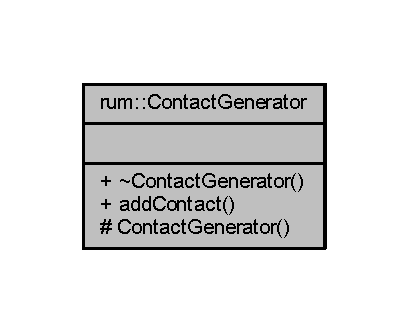
\includegraphics[width=196pt]{classrum_1_1_contact_generator__coll__graph}
\end{center}
\end{figure}
\subsection*{Public Member Functions}
\begin{DoxyCompactItemize}
\item 
virtual \mbox{\hyperlink{classrum_1_1_contact_generator_acbd18056803ce7fd435a7a9505ce96ab}{$\sim$\+Contact\+Generator}} ()
\item 
virtual unsigned \mbox{\hyperlink{classrum_1_1_contact_generator_a10e14c5da23ed3fa91a6abac2f133b72}{add\+Contact}} (\mbox{\hyperlink{classrum_1_1_contact}{Contact}} $\ast$contact, unsigned limit) const
\end{DoxyCompactItemize}
\subsection*{Protected Member Functions}
\begin{DoxyCompactItemize}
\item 
\mbox{\hyperlink{classrum_1_1_contact_generator_a0c509abdf4d3eda20983e452d7c493c9}{Contact\+Generator}} ()
\end{DoxyCompactItemize}


\subsection{Constructor \& Destructor Documentation}
\mbox{\Hypertarget{classrum_1_1_contact_generator_acbd18056803ce7fd435a7a9505ce96ab}\label{classrum_1_1_contact_generator_acbd18056803ce7fd435a7a9505ce96ab}} 
\index{rum\+::\+Contact\+Generator@{rum\+::\+Contact\+Generator}!````~Contact\+Generator@{$\sim$\+Contact\+Generator}}
\index{````~Contact\+Generator@{$\sim$\+Contact\+Generator}!rum\+::\+Contact\+Generator@{rum\+::\+Contact\+Generator}}
\subsubsection{\texorpdfstring{$\sim$\+Contact\+Generator()}{~ContactGenerator()}}
{\footnotesize\ttfamily rum\+::\+Contact\+Generator\+::$\sim$\+Contact\+Generator (\begin{DoxyParamCaption}{ }\end{DoxyParamCaption})\hspace{0.3cm}{\ttfamily [virtual]}, {\ttfamily [default]}}

\mbox{\Hypertarget{classrum_1_1_contact_generator_a0c509abdf4d3eda20983e452d7c493c9}\label{classrum_1_1_contact_generator_a0c509abdf4d3eda20983e452d7c493c9}} 
\index{rum\+::\+Contact\+Generator@{rum\+::\+Contact\+Generator}!Contact\+Generator@{Contact\+Generator}}
\index{Contact\+Generator@{Contact\+Generator}!rum\+::\+Contact\+Generator@{rum\+::\+Contact\+Generator}}
\subsubsection{\texorpdfstring{Contact\+Generator()}{ContactGenerator()}}
{\footnotesize\ttfamily rum\+::\+Contact\+Generator\+::\+Contact\+Generator (\begin{DoxyParamCaption}{ }\end{DoxyParamCaption})\hspace{0.3cm}{\ttfamily [explicit]}, {\ttfamily [protected]}, {\ttfamily [default]}}



\subsection{Member Function Documentation}
\mbox{\Hypertarget{classrum_1_1_contact_generator_a10e14c5da23ed3fa91a6abac2f133b72}\label{classrum_1_1_contact_generator_a10e14c5da23ed3fa91a6abac2f133b72}} 
\index{rum\+::\+Contact\+Generator@{rum\+::\+Contact\+Generator}!add\+Contact@{add\+Contact}}
\index{add\+Contact@{add\+Contact}!rum\+::\+Contact\+Generator@{rum\+::\+Contact\+Generator}}
\subsubsection{\texorpdfstring{add\+Contact()}{addContact()}}
{\footnotesize\ttfamily virtual unsigned rum\+::\+Contact\+Generator\+::add\+Contact (\begin{DoxyParamCaption}\item[{\mbox{\hyperlink{classrum_1_1_contact}{Contact}} $\ast$}]{contact,  }\item[{unsigned}]{limit }\end{DoxyParamCaption}) const\hspace{0.3cm}{\ttfamily [virtual]}}



The documentation for this class was generated from the following files\+:\begin{DoxyCompactItemize}
\item 
D\+:/\+Library/\+Documents/\+Job/\+Forschungsmaster/\+Projekte/\+Rumble3\+D/\+Rumble3\+D/include/\+R3\+D/\+Rigid\+Body\+Engine/\mbox{\hyperlink{_contact_generator_8h}{Contact\+Generator.\+h}}\item 
D\+:/\+Library/\+Documents/\+Job/\+Forschungsmaster/\+Projekte/\+Rumble3\+D/\+Rumble3\+D/src/\+Rigid\+Body\+Engine/\mbox{\hyperlink{_contact_generator_8cpp}{Contact\+Generator.\+cpp}}\end{DoxyCompactItemize}

\hypertarget{classrum_1_1_contact_resolver}{}\section{rum\+:\+:Contact\+Resolver Class Reference}
\label{classrum_1_1_contact_resolver}\index{rum\+::\+Contact\+Resolver@{rum\+::\+Contact\+Resolver}}


{\ttfamily \#include $<$Contact\+Resolver.\+h$>$}



Collaboration diagram for rum\+:\+:Contact\+Resolver\+:\nopagebreak
\begin{figure}[H]
\begin{center}
\leavevmode
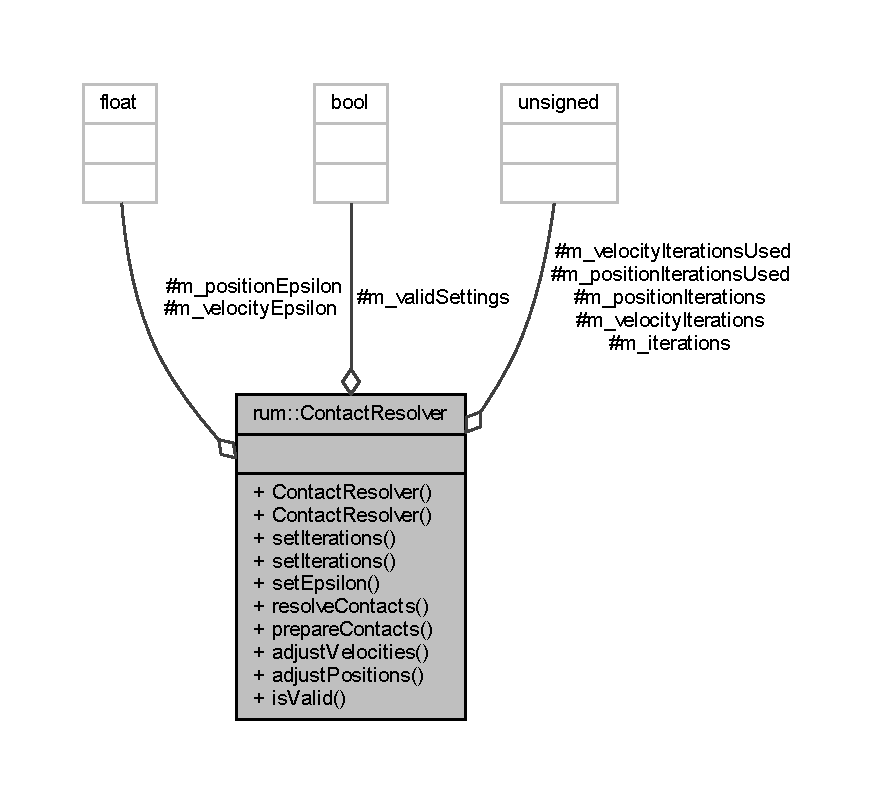
\includegraphics[width=350pt]{classrum_1_1_contact_resolver__coll__graph}
\end{center}
\end{figure}
\subsection*{Public Member Functions}
\begin{DoxyCompactItemize}
\item 
\hyperlink{classrum_1_1_contact_resolver_adaf1fa2fd7b845fb3b0496505074bd01}{Contact\+Resolver} (unsigned iterations, \hyperlink{namespacerum_a7e8cca23573d5eaead0f138cbaa4862c}{real} velocity\+Epsilon=\hyperlink{namespacerum_a7e8cca23573d5eaead0f138cbaa4862c}{real}(0.\+01f), real position\+Epsilon=real(0.\+01f))
\item 
\hyperlink{classrum_1_1_contact_resolver_a0d517774fa736afb5eb9098a5051761a}{Contact\+Resolver} (unsigned velocity\+Iterations, unsigned position\+Iterations, \hyperlink{namespacerum_a7e8cca23573d5eaead0f138cbaa4862c}{real} velocity\+Epsilon=\hyperlink{namespacerum_a7e8cca23573d5eaead0f138cbaa4862c}{real}(0.\+01f), real position\+Epsilon=real(0.\+01f))
\item 
void \hyperlink{classrum_1_1_contact_resolver_a22500b8327332e7c95c100aa30160ff8}{set\+Iterations} (unsigned iterations)
\item 
void \hyperlink{classrum_1_1_contact_resolver_a2dd2bf231348dc011449f43e71087182}{set\+Iterations} (unsigned velocity\+Iterations, unsigned position\+Iterations)
\item 
void \hyperlink{classrum_1_1_contact_resolver_a6dd5b9d5e4057068fd96fff89a607bcc}{set\+Epsilon} (\hyperlink{namespacerum_a7e8cca23573d5eaead0f138cbaa4862c}{real} velocity\+Epsilon, \hyperlink{namespacerum_a7e8cca23573d5eaead0f138cbaa4862c}{real} position\+Epsilon)
\item 
void \hyperlink{classrum_1_1_contact_resolver_a153040b39293571645cd24ab2dfb763a}{resolve\+Contacts} (\hyperlink{classrum_1_1_contact}{Contact} $\ast$contacts, unsigned num\+Contacts, \hyperlink{namespacerum_a7e8cca23573d5eaead0f138cbaa4862c}{real} duration)
\item 
void \hyperlink{classrum_1_1_contact_resolver_aa1171defbfc3b06d84a7221666198aaf}{prepare\+Contacts} (\hyperlink{classrum_1_1_contact}{Contact} $\ast$contacts, unsigned num\+Contacts, \hyperlink{namespacerum_a7e8cca23573d5eaead0f138cbaa4862c}{real} duration)
\item 
void \hyperlink{classrum_1_1_contact_resolver_a9a76b0e81743999eea3c0ec882960d4c}{adjust\+Velocities} (\hyperlink{classrum_1_1_contact}{Contact} $\ast$c, unsigned num\+Contacts, \hyperlink{namespacerum_a7e8cca23573d5eaead0f138cbaa4862c}{real} duration)
\item 
void \hyperlink{classrum_1_1_contact_resolver_a6900a5545bde3995302f22bdb7c85934}{adjust\+Positions} (\hyperlink{classrum_1_1_contact}{Contact} $\ast$c, unsigned num\+Contacts, \hyperlink{namespacerum_a7e8cca23573d5eaead0f138cbaa4862c}{real} duration)
\item 
bool \hyperlink{classrum_1_1_contact_resolver_ab5331d0189d4d9fe1c17622638a8b0e5}{is\+Valid} ()
\end{DoxyCompactItemize}
\subsection*{Protected Attributes}
\begin{DoxyCompactItemize}
\item 
unsigned \hyperlink{classrum_1_1_contact_resolver_a69b94c3b3bffe713655ed4b2209d17c3}{m\+\_\+velocity\+Iterations}
\item 
unsigned \hyperlink{classrum_1_1_contact_resolver_adb8b6bf74fdb76f502f412b947a6b6b9}{m\+\_\+position\+Iterations}
\item 
\hyperlink{namespacerum_a7e8cca23573d5eaead0f138cbaa4862c}{real} \hyperlink{classrum_1_1_contact_resolver_a2bd8f6cd976d45ce1fb8407c58d68e96}{m\+\_\+velocity\+Epsilon}
\item 
\hyperlink{namespacerum_a7e8cca23573d5eaead0f138cbaa4862c}{real} \hyperlink{classrum_1_1_contact_resolver_a7de7422d90c874c9b3852fb98612c6ce}{m\+\_\+position\+Epsilon}
\item 
unsigned \hyperlink{classrum_1_1_contact_resolver_a1f26bcb510350f094a9488c09125bcd7}{m\+\_\+velocity\+Iterations\+Used}
\item 
unsigned \hyperlink{classrum_1_1_contact_resolver_ad71be20b842af92754adcf9310a54fd6}{m\+\_\+position\+Iterations\+Used}
\item 
bool \hyperlink{classrum_1_1_contact_resolver_ab96daf85e76174045aada60b973bea4f}{m\+\_\+valid\+Settings}
\end{DoxyCompactItemize}


\subsection{Constructor \& Destructor Documentation}
\mbox{\Hypertarget{classrum_1_1_contact_resolver_adaf1fa2fd7b845fb3b0496505074bd01}\label{classrum_1_1_contact_resolver_adaf1fa2fd7b845fb3b0496505074bd01}} 
\index{rum\+::\+Contact\+Resolver@{rum\+::\+Contact\+Resolver}!Contact\+Resolver@{Contact\+Resolver}}
\index{Contact\+Resolver@{Contact\+Resolver}!rum\+::\+Contact\+Resolver@{rum\+::\+Contact\+Resolver}}
\subsubsection{\texorpdfstring{Contact\+Resolver()}{ContactResolver()}\hspace{0.1cm}{\footnotesize\ttfamily [1/2]}}
{\footnotesize\ttfamily rum\+::\+Contact\+Resolver\+::\+Contact\+Resolver (\begin{DoxyParamCaption}\item[{unsigned}]{iterations,  }\item[{\hyperlink{namespacerum_a7e8cca23573d5eaead0f138cbaa4862c}{real}}]{velocity\+Epsilon = {\ttfamily \hyperlink{namespacerum_a7e8cca23573d5eaead0f138cbaa4862c}{real}(0.01f)},  }\item[{\hyperlink{namespacerum_a7e8cca23573d5eaead0f138cbaa4862c}{real}}]{position\+Epsilon = {\ttfamily \hyperlink{namespacerum_a7e8cca23573d5eaead0f138cbaa4862c}{real}(0.01f)} }\end{DoxyParamCaption})}

Creates a new contact resolver with the given number of iterations per resolution call, and optional epsilon values. \mbox{\Hypertarget{classrum_1_1_contact_resolver_a0d517774fa736afb5eb9098a5051761a}\label{classrum_1_1_contact_resolver_a0d517774fa736afb5eb9098a5051761a}} 
\index{rum\+::\+Contact\+Resolver@{rum\+::\+Contact\+Resolver}!Contact\+Resolver@{Contact\+Resolver}}
\index{Contact\+Resolver@{Contact\+Resolver}!rum\+::\+Contact\+Resolver@{rum\+::\+Contact\+Resolver}}
\subsubsection{\texorpdfstring{Contact\+Resolver()}{ContactResolver()}\hspace{0.1cm}{\footnotesize\ttfamily [2/2]}}
{\footnotesize\ttfamily rum\+::\+Contact\+Resolver\+::\+Contact\+Resolver (\begin{DoxyParamCaption}\item[{unsigned}]{velocity\+Iterations,  }\item[{unsigned}]{position\+Iterations,  }\item[{\hyperlink{namespacerum_a7e8cca23573d5eaead0f138cbaa4862c}{real}}]{velocity\+Epsilon = {\ttfamily \hyperlink{namespacerum_a7e8cca23573d5eaead0f138cbaa4862c}{real}(0.01f)},  }\item[{\hyperlink{namespacerum_a7e8cca23573d5eaead0f138cbaa4862c}{real}}]{position\+Epsilon = {\ttfamily \hyperlink{namespacerum_a7e8cca23573d5eaead0f138cbaa4862c}{real}(0.01f)} }\end{DoxyParamCaption})}

Creates a new contact resolver with the given number of iterations for each kind of resolution, and optional epsilon values. 

\subsection{Member Function Documentation}
\mbox{\Hypertarget{classrum_1_1_contact_resolver_a6900a5545bde3995302f22bdb7c85934}\label{classrum_1_1_contact_resolver_a6900a5545bde3995302f22bdb7c85934}} 
\index{rum\+::\+Contact\+Resolver@{rum\+::\+Contact\+Resolver}!adjust\+Positions@{adjust\+Positions}}
\index{adjust\+Positions@{adjust\+Positions}!rum\+::\+Contact\+Resolver@{rum\+::\+Contact\+Resolver}}
\subsubsection{\texorpdfstring{adjust\+Positions()}{adjustPositions()}}
{\footnotesize\ttfamily void rum\+::\+Contact\+Resolver\+::adjust\+Positions (\begin{DoxyParamCaption}\item[{\hyperlink{classrum_1_1_contact}{Contact} $\ast$}]{c,  }\item[{unsigned}]{num\+Contacts,  }\item[{\hyperlink{namespacerum_a7e8cca23573d5eaead0f138cbaa4862c}{real}}]{duration }\end{DoxyParamCaption})}

\mbox{\Hypertarget{classrum_1_1_contact_resolver_a9a76b0e81743999eea3c0ec882960d4c}\label{classrum_1_1_contact_resolver_a9a76b0e81743999eea3c0ec882960d4c}} 
\index{rum\+::\+Contact\+Resolver@{rum\+::\+Contact\+Resolver}!adjust\+Velocities@{adjust\+Velocities}}
\index{adjust\+Velocities@{adjust\+Velocities}!rum\+::\+Contact\+Resolver@{rum\+::\+Contact\+Resolver}}
\subsubsection{\texorpdfstring{adjust\+Velocities()}{adjustVelocities()}}
{\footnotesize\ttfamily void rum\+::\+Contact\+Resolver\+::adjust\+Velocities (\begin{DoxyParamCaption}\item[{\hyperlink{classrum_1_1_contact}{Contact} $\ast$}]{c,  }\item[{unsigned}]{num\+Contacts,  }\item[{\hyperlink{namespacerum_a7e8cca23573d5eaead0f138cbaa4862c}{real}}]{duration }\end{DoxyParamCaption})}

\mbox{\Hypertarget{classrum_1_1_contact_resolver_ab5331d0189d4d9fe1c17622638a8b0e5}\label{classrum_1_1_contact_resolver_ab5331d0189d4d9fe1c17622638a8b0e5}} 
\index{rum\+::\+Contact\+Resolver@{rum\+::\+Contact\+Resolver}!is\+Valid@{is\+Valid}}
\index{is\+Valid@{is\+Valid}!rum\+::\+Contact\+Resolver@{rum\+::\+Contact\+Resolver}}
\subsubsection{\texorpdfstring{is\+Valid()}{isValid()}}
{\footnotesize\ttfamily bool rum\+::\+Contact\+Resolver\+::is\+Valid (\begin{DoxyParamCaption}{ }\end{DoxyParamCaption})}

\mbox{\Hypertarget{classrum_1_1_contact_resolver_aa1171defbfc3b06d84a7221666198aaf}\label{classrum_1_1_contact_resolver_aa1171defbfc3b06d84a7221666198aaf}} 
\index{rum\+::\+Contact\+Resolver@{rum\+::\+Contact\+Resolver}!prepare\+Contacts@{prepare\+Contacts}}
\index{prepare\+Contacts@{prepare\+Contacts}!rum\+::\+Contact\+Resolver@{rum\+::\+Contact\+Resolver}}
\subsubsection{\texorpdfstring{prepare\+Contacts()}{prepareContacts()}}
{\footnotesize\ttfamily void rum\+::\+Contact\+Resolver\+::prepare\+Contacts (\begin{DoxyParamCaption}\item[{\hyperlink{classrum_1_1_contact}{Contact} $\ast$}]{contacts,  }\item[{unsigned}]{num\+Contacts,  }\item[{\hyperlink{namespacerum_a7e8cca23573d5eaead0f138cbaa4862c}{real}}]{duration }\end{DoxyParamCaption})}

\mbox{\Hypertarget{classrum_1_1_contact_resolver_a153040b39293571645cd24ab2dfb763a}\label{classrum_1_1_contact_resolver_a153040b39293571645cd24ab2dfb763a}} 
\index{rum\+::\+Contact\+Resolver@{rum\+::\+Contact\+Resolver}!resolve\+Contacts@{resolve\+Contacts}}
\index{resolve\+Contacts@{resolve\+Contacts}!rum\+::\+Contact\+Resolver@{rum\+::\+Contact\+Resolver}}
\subsubsection{\texorpdfstring{resolve\+Contacts()}{resolveContacts()}}
{\footnotesize\ttfamily void rum\+::\+Contact\+Resolver\+::resolve\+Contacts (\begin{DoxyParamCaption}\item[{\hyperlink{classrum_1_1_contact}{Contact} $\ast$}]{contacts,  }\item[{unsigned}]{num\+Contacts,  }\item[{\hyperlink{namespacerum_a7e8cca23573d5eaead0f138cbaa4862c}{real}}]{duration }\end{DoxyParamCaption})}

\mbox{\Hypertarget{classrum_1_1_contact_resolver_a6dd5b9d5e4057068fd96fff89a607bcc}\label{classrum_1_1_contact_resolver_a6dd5b9d5e4057068fd96fff89a607bcc}} 
\index{rum\+::\+Contact\+Resolver@{rum\+::\+Contact\+Resolver}!set\+Epsilon@{set\+Epsilon}}
\index{set\+Epsilon@{set\+Epsilon}!rum\+::\+Contact\+Resolver@{rum\+::\+Contact\+Resolver}}
\subsubsection{\texorpdfstring{set\+Epsilon()}{setEpsilon()}}
{\footnotesize\ttfamily void rum\+::\+Contact\+Resolver\+::set\+Epsilon (\begin{DoxyParamCaption}\item[{\hyperlink{namespacerum_a7e8cca23573d5eaead0f138cbaa4862c}{real}}]{velocity\+Epsilon,  }\item[{\hyperlink{namespacerum_a7e8cca23573d5eaead0f138cbaa4862c}{real}}]{position\+Epsilon }\end{DoxyParamCaption})}

\mbox{\Hypertarget{classrum_1_1_contact_resolver_a22500b8327332e7c95c100aa30160ff8}\label{classrum_1_1_contact_resolver_a22500b8327332e7c95c100aa30160ff8}} 
\index{rum\+::\+Contact\+Resolver@{rum\+::\+Contact\+Resolver}!set\+Iterations@{set\+Iterations}}
\index{set\+Iterations@{set\+Iterations}!rum\+::\+Contact\+Resolver@{rum\+::\+Contact\+Resolver}}
\subsubsection{\texorpdfstring{set\+Iterations()}{setIterations()}\hspace{0.1cm}{\footnotesize\ttfamily [1/2]}}
{\footnotesize\ttfamily void rum\+::\+Contact\+Resolver\+::set\+Iterations (\begin{DoxyParamCaption}\item[{unsigned}]{iterations }\end{DoxyParamCaption})}

\mbox{\Hypertarget{classrum_1_1_contact_resolver_a2dd2bf231348dc011449f43e71087182}\label{classrum_1_1_contact_resolver_a2dd2bf231348dc011449f43e71087182}} 
\index{rum\+::\+Contact\+Resolver@{rum\+::\+Contact\+Resolver}!set\+Iterations@{set\+Iterations}}
\index{set\+Iterations@{set\+Iterations}!rum\+::\+Contact\+Resolver@{rum\+::\+Contact\+Resolver}}
\subsubsection{\texorpdfstring{set\+Iterations()}{setIterations()}\hspace{0.1cm}{\footnotesize\ttfamily [2/2]}}
{\footnotesize\ttfamily void rum\+::\+Contact\+Resolver\+::set\+Iterations (\begin{DoxyParamCaption}\item[{unsigned}]{velocity\+Iterations,  }\item[{unsigned}]{position\+Iterations }\end{DoxyParamCaption})}



\subsection{Member Data Documentation}
\mbox{\Hypertarget{classrum_1_1_contact_resolver_a7de7422d90c874c9b3852fb98612c6ce}\label{classrum_1_1_contact_resolver_a7de7422d90c874c9b3852fb98612c6ce}} 
\index{rum\+::\+Contact\+Resolver@{rum\+::\+Contact\+Resolver}!m\+\_\+position\+Epsilon@{m\+\_\+position\+Epsilon}}
\index{m\+\_\+position\+Epsilon@{m\+\_\+position\+Epsilon}!rum\+::\+Contact\+Resolver@{rum\+::\+Contact\+Resolver}}
\subsubsection{\texorpdfstring{m\+\_\+position\+Epsilon}{m\_positionEpsilon}}
{\footnotesize\ttfamily \hyperlink{namespacerum_a7e8cca23573d5eaead0f138cbaa4862c}{real} rum\+::\+Contact\+Resolver\+::m\+\_\+position\+Epsilon\hspace{0.3cm}{\ttfamily [protected]}}

To avoid instability penetrations smaller than this value are considered to be not interpenetrating. Too small and the simulation may be unstable, too large and the bodies may interpenetrate visually. A good starting point is the default of0.\+01. \mbox{\Hypertarget{classrum_1_1_contact_resolver_adb8b6bf74fdb76f502f412b947a6b6b9}\label{classrum_1_1_contact_resolver_adb8b6bf74fdb76f502f412b947a6b6b9}} 
\index{rum\+::\+Contact\+Resolver@{rum\+::\+Contact\+Resolver}!m\+\_\+position\+Iterations@{m\+\_\+position\+Iterations}}
\index{m\+\_\+position\+Iterations@{m\+\_\+position\+Iterations}!rum\+::\+Contact\+Resolver@{rum\+::\+Contact\+Resolver}}
\subsubsection{\texorpdfstring{m\+\_\+position\+Iterations}{m\_positionIterations}}
{\footnotesize\ttfamily unsigned rum\+::\+Contact\+Resolver\+::m\+\_\+position\+Iterations\hspace{0.3cm}{\ttfamily [protected]}}

Holds the number of iterations to perform when resolving position. \mbox{\Hypertarget{classrum_1_1_contact_resolver_ad71be20b842af92754adcf9310a54fd6}\label{classrum_1_1_contact_resolver_ad71be20b842af92754adcf9310a54fd6}} 
\index{rum\+::\+Contact\+Resolver@{rum\+::\+Contact\+Resolver}!m\+\_\+position\+Iterations\+Used@{m\+\_\+position\+Iterations\+Used}}
\index{m\+\_\+position\+Iterations\+Used@{m\+\_\+position\+Iterations\+Used}!rum\+::\+Contact\+Resolver@{rum\+::\+Contact\+Resolver}}
\subsubsection{\texorpdfstring{m\+\_\+position\+Iterations\+Used}{m\_positionIterationsUsed}}
{\footnotesize\ttfamily unsigned rum\+::\+Contact\+Resolver\+::m\+\_\+position\+Iterations\+Used\hspace{0.3cm}{\ttfamily [protected]}}

Stores the number of position iterations used in the last call to resolve contacts. \mbox{\Hypertarget{classrum_1_1_contact_resolver_ab96daf85e76174045aada60b973bea4f}\label{classrum_1_1_contact_resolver_ab96daf85e76174045aada60b973bea4f}} 
\index{rum\+::\+Contact\+Resolver@{rum\+::\+Contact\+Resolver}!m\+\_\+valid\+Settings@{m\+\_\+valid\+Settings}}
\index{m\+\_\+valid\+Settings@{m\+\_\+valid\+Settings}!rum\+::\+Contact\+Resolver@{rum\+::\+Contact\+Resolver}}
\subsubsection{\texorpdfstring{m\+\_\+valid\+Settings}{m\_validSettings}}
{\footnotesize\ttfamily bool rum\+::\+Contact\+Resolver\+::m\+\_\+valid\+Settings\hspace{0.3cm}{\ttfamily [protected]}}

Keeps track of whether the internal settings are valid. \mbox{\Hypertarget{classrum_1_1_contact_resolver_a2bd8f6cd976d45ce1fb8407c58d68e96}\label{classrum_1_1_contact_resolver_a2bd8f6cd976d45ce1fb8407c58d68e96}} 
\index{rum\+::\+Contact\+Resolver@{rum\+::\+Contact\+Resolver}!m\+\_\+velocity\+Epsilon@{m\+\_\+velocity\+Epsilon}}
\index{m\+\_\+velocity\+Epsilon@{m\+\_\+velocity\+Epsilon}!rum\+::\+Contact\+Resolver@{rum\+::\+Contact\+Resolver}}
\subsubsection{\texorpdfstring{m\+\_\+velocity\+Epsilon}{m\_velocityEpsilon}}
{\footnotesize\ttfamily \hyperlink{namespacerum_a7e8cca23573d5eaead0f138cbaa4862c}{real} rum\+::\+Contact\+Resolver\+::m\+\_\+velocity\+Epsilon\hspace{0.3cm}{\ttfamily [protected]}}

To avoid instability velocities smaller than this value are considered to be zero. Too small and the simulation may be unstable, too large and the bodies may interpenetrate visually. A good starting point is the default of 0.\+01. \mbox{\Hypertarget{classrum_1_1_contact_resolver_a69b94c3b3bffe713655ed4b2209d17c3}\label{classrum_1_1_contact_resolver_a69b94c3b3bffe713655ed4b2209d17c3}} 
\index{rum\+::\+Contact\+Resolver@{rum\+::\+Contact\+Resolver}!m\+\_\+velocity\+Iterations@{m\+\_\+velocity\+Iterations}}
\index{m\+\_\+velocity\+Iterations@{m\+\_\+velocity\+Iterations}!rum\+::\+Contact\+Resolver@{rum\+::\+Contact\+Resolver}}
\subsubsection{\texorpdfstring{m\+\_\+velocity\+Iterations}{m\_velocityIterations}}
{\footnotesize\ttfamily unsigned rum\+::\+Contact\+Resolver\+::m\+\_\+velocity\+Iterations\hspace{0.3cm}{\ttfamily [protected]}}

Holds the number of iterations to perform when resolving velocity. \mbox{\Hypertarget{classrum_1_1_contact_resolver_a1f26bcb510350f094a9488c09125bcd7}\label{classrum_1_1_contact_resolver_a1f26bcb510350f094a9488c09125bcd7}} 
\index{rum\+::\+Contact\+Resolver@{rum\+::\+Contact\+Resolver}!m\+\_\+velocity\+Iterations\+Used@{m\+\_\+velocity\+Iterations\+Used}}
\index{m\+\_\+velocity\+Iterations\+Used@{m\+\_\+velocity\+Iterations\+Used}!rum\+::\+Contact\+Resolver@{rum\+::\+Contact\+Resolver}}
\subsubsection{\texorpdfstring{m\+\_\+velocity\+Iterations\+Used}{m\_velocityIterationsUsed}}
{\footnotesize\ttfamily unsigned rum\+::\+Contact\+Resolver\+::m\+\_\+velocity\+Iterations\+Used\hspace{0.3cm}{\ttfamily [protected]}}

Stores the number of velocity iterations used in the last call to resolve contacts. 

The documentation for this class was generated from the following files\+:\begin{DoxyCompactItemize}
\item 
F\+:/\+Library/\+Documents/\+Job/\+Forschungsmaster/\+Rumble3\+D/\+Rumble3\+D/include/\+R3\+D/\+Rigid\+Body\+Engine/\hyperlink{_contact_resolver_8h}{Contact\+Resolver.\+h}\item 
F\+:/\+Library/\+Documents/\+Job/\+Forschungsmaster/\+Rumble3\+D/\+Rumble3\+D/src/\+Rigid\+Body\+Engine/\hyperlink{_contact_resolver_8cpp}{Contact\+Resolver.\+cpp}\end{DoxyCompactItemize}

\hypertarget{classrum_1_1_directed_force}{}\section{rum\+:\+:Directed\+Force Class Reference}
\label{classrum_1_1_directed_force}\index{rum\+::\+Directed\+Force@{rum\+::\+Directed\+Force}}


{\ttfamily \#include $<$Directed\+Force.\+h$>$}



Inheritance diagram for rum\+:\+:Directed\+Force\+:\nopagebreak
\begin{figure}[H]
\begin{center}
\leavevmode
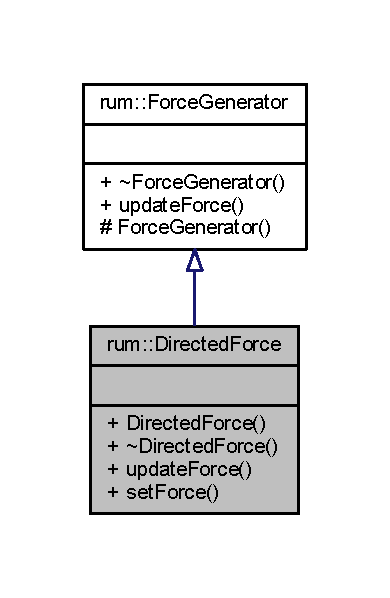
\includegraphics[width=187pt]{classrum_1_1_directed_force__inherit__graph}
\end{center}
\end{figure}


Collaboration diagram for rum\+:\+:Directed\+Force\+:\nopagebreak
\begin{figure}[H]
\begin{center}
\leavevmode
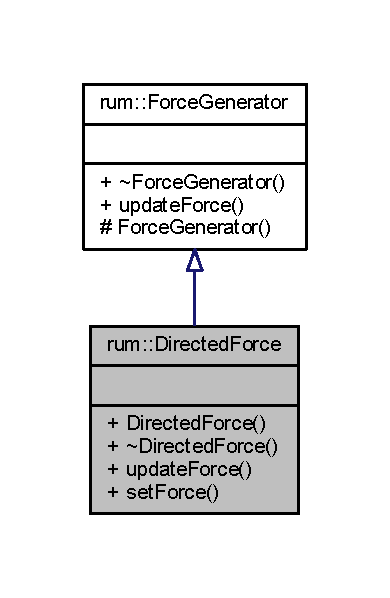
\includegraphics[width=187pt]{classrum_1_1_directed_force__coll__graph}
\end{center}
\end{figure}
\subsection*{Public Member Functions}
\begin{DoxyCompactItemize}
\item 
\hyperlink{classrum_1_1_directed_force_ac6be6fbfe8f21ed2c6c3cf050ac180b8}{Directed\+Force} (glm\+::vec3 local\+Position, glm\+::vec3 force)
\item 
\hyperlink{classrum_1_1_directed_force_a6da6baf550b205f22f3c95d7140334c0}{$\sim$\+Directed\+Force} ()
\item 
void \hyperlink{classrum_1_1_directed_force_a79b53d849f80fb69ca1fa42ea43829b4}{Update\+Force} (\hyperlink{classrum_1_1_rigid_body}{Rigid\+Body} $\ast$body, \hyperlink{namespacerum_a7e8cca23573d5eaead0f138cbaa4862c}{real} duration) override
\item 
void \hyperlink{classrum_1_1_directed_force_ae632c56c26193e81ff71501dab5b8e04}{Set\+Force} (const glm\+::vec3 \&force)
\end{DoxyCompactItemize}


\subsection{Constructor \& Destructor Documentation}
\mbox{\Hypertarget{classrum_1_1_directed_force_ac6be6fbfe8f21ed2c6c3cf050ac180b8}\label{classrum_1_1_directed_force_ac6be6fbfe8f21ed2c6c3cf050ac180b8}} 
\index{rum\+::\+Directed\+Force@{rum\+::\+Directed\+Force}!Directed\+Force@{Directed\+Force}}
\index{Directed\+Force@{Directed\+Force}!rum\+::\+Directed\+Force@{rum\+::\+Directed\+Force}}
\subsubsection{\texorpdfstring{Directed\+Force()}{DirectedForce()}}
{\footnotesize\ttfamily rum\+::\+Directed\+Force\+::\+Directed\+Force (\begin{DoxyParamCaption}\item[{glm\+::vec3}]{local\+Position,  }\item[{glm\+::vec3}]{force }\end{DoxyParamCaption})}

\mbox{\Hypertarget{classrum_1_1_directed_force_a6da6baf550b205f22f3c95d7140334c0}\label{classrum_1_1_directed_force_a6da6baf550b205f22f3c95d7140334c0}} 
\index{rum\+::\+Directed\+Force@{rum\+::\+Directed\+Force}!````~Directed\+Force@{$\sim$\+Directed\+Force}}
\index{````~Directed\+Force@{$\sim$\+Directed\+Force}!rum\+::\+Directed\+Force@{rum\+::\+Directed\+Force}}
\subsubsection{\texorpdfstring{$\sim$\+Directed\+Force()}{~DirectedForce()}}
{\footnotesize\ttfamily rum\+::\+Directed\+Force\+::$\sim$\+Directed\+Force (\begin{DoxyParamCaption}{ }\end{DoxyParamCaption})}



\subsection{Member Function Documentation}
\mbox{\Hypertarget{classrum_1_1_directed_force_ae632c56c26193e81ff71501dab5b8e04}\label{classrum_1_1_directed_force_ae632c56c26193e81ff71501dab5b8e04}} 
\index{rum\+::\+Directed\+Force@{rum\+::\+Directed\+Force}!Set\+Force@{Set\+Force}}
\index{Set\+Force@{Set\+Force}!rum\+::\+Directed\+Force@{rum\+::\+Directed\+Force}}
\subsubsection{\texorpdfstring{Set\+Force()}{SetForce()}}
{\footnotesize\ttfamily void rum\+::\+Directed\+Force\+::\+Set\+Force (\begin{DoxyParamCaption}\item[{const glm\+::vec3 \&}]{force }\end{DoxyParamCaption})}

\mbox{\Hypertarget{classrum_1_1_directed_force_a79b53d849f80fb69ca1fa42ea43829b4}\label{classrum_1_1_directed_force_a79b53d849f80fb69ca1fa42ea43829b4}} 
\index{rum\+::\+Directed\+Force@{rum\+::\+Directed\+Force}!Update\+Force@{Update\+Force}}
\index{Update\+Force@{Update\+Force}!rum\+::\+Directed\+Force@{rum\+::\+Directed\+Force}}
\subsubsection{\texorpdfstring{Update\+Force()}{UpdateForce()}}
{\footnotesize\ttfamily void rum\+::\+Directed\+Force\+::\+Update\+Force (\begin{DoxyParamCaption}\item[{\hyperlink{classrum_1_1_rigid_body}{Rigid\+Body} $\ast$}]{body,  }\item[{\hyperlink{namespacerum_a7e8cca23573d5eaead0f138cbaa4862c}{real}}]{duration }\end{DoxyParamCaption})\hspace{0.3cm}{\ttfamily [override]}, {\ttfamily [virtual]}}



Implements \hyperlink{classrum_1_1_force_generator_a6b038c9a39e4cf64b2dcf2741804a824}{rum\+::\+Force\+Generator}.



The documentation for this class was generated from the following files\+:\begin{DoxyCompactItemize}
\item 
F\+:/\+Library/\+Documents/\+Job/\+Forschungsmaster/\+Rumble3\+D/\+Rumble3\+D/include/\+R3\+D/\+Rigid\+Body\+Engine/\hyperlink{_directed_force_8h}{Directed\+Force.\+h}\item 
F\+:/\+Library/\+Documents/\+Job/\+Forschungsmaster/\+Rumble3\+D/\+Rumble3\+D/src/\+Rigid\+Body\+Engine/\hyperlink{_directed_force_8cpp}{Directed\+Force.\+cpp}\end{DoxyCompactItemize}

\hypertarget{classrum_1_1_force_generator}{}\section{rum\+:\+:Force\+Generator Class Reference}
\label{classrum_1_1_force_generator}\index{rum\+::\+Force\+Generator@{rum\+::\+Force\+Generator}}


{\ttfamily \#include $<$Force\+Generator.\+h$>$}



Inheritance diagram for rum\+:\+:Force\+Generator\+:\nopagebreak
\begin{figure}[H]
\begin{center}
\leavevmode
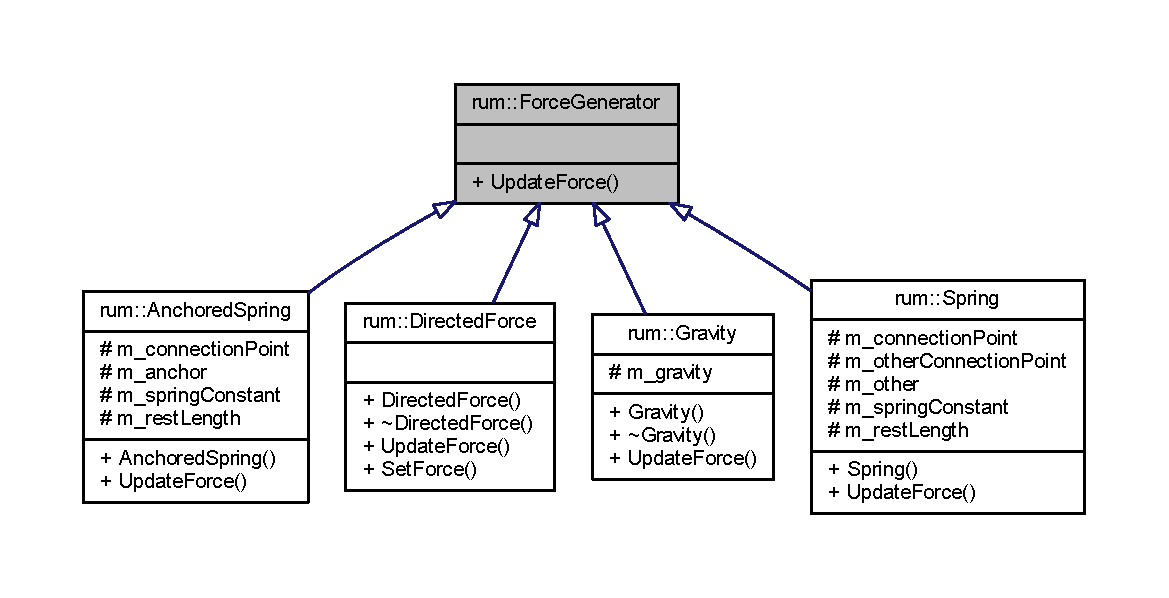
\includegraphics[width=350pt]{classrum_1_1_force_generator__inherit__graph}
\end{center}
\end{figure}


Collaboration diagram for rum\+:\+:Force\+Generator\+:\nopagebreak
\begin{figure}[H]
\begin{center}
\leavevmode
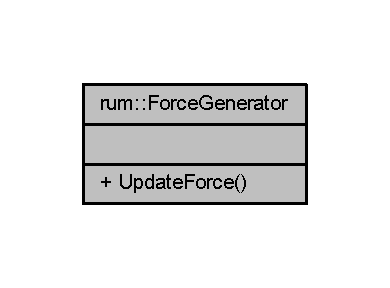
\includegraphics[width=187pt]{classrum_1_1_force_generator__coll__graph}
\end{center}
\end{figure}
\subsection*{Public Member Functions}
\begin{DoxyCompactItemize}
\item 
virtual void \hyperlink{classrum_1_1_force_generator_a6b038c9a39e4cf64b2dcf2741804a824}{Update\+Force} (\hyperlink{classrum_1_1_rigid_body}{Rigid\+Body} $\ast$body, \hyperlink{namespacerum_a7e8cca23573d5eaead0f138cbaa4862c}{real} duration)=0
\end{DoxyCompactItemize}


\subsection{Member Function Documentation}
\mbox{\Hypertarget{classrum_1_1_force_generator_a6b038c9a39e4cf64b2dcf2741804a824}\label{classrum_1_1_force_generator_a6b038c9a39e4cf64b2dcf2741804a824}} 
\index{rum\+::\+Force\+Generator@{rum\+::\+Force\+Generator}!Update\+Force@{Update\+Force}}
\index{Update\+Force@{Update\+Force}!rum\+::\+Force\+Generator@{rum\+::\+Force\+Generator}}
\subsubsection{\texorpdfstring{Update\+Force()}{UpdateForce()}}
{\footnotesize\ttfamily virtual void rum\+::\+Force\+Generator\+::\+Update\+Force (\begin{DoxyParamCaption}\item[{\hyperlink{classrum_1_1_rigid_body}{Rigid\+Body} $\ast$}]{body,  }\item[{\hyperlink{namespacerum_a7e8cca23573d5eaead0f138cbaa4862c}{real}}]{duration }\end{DoxyParamCaption})\hspace{0.3cm}{\ttfamily [pure virtual]}}



Implemented in \hyperlink{classrum_1_1_spring_ac9c58b1740f347199669132722b998af}{rum\+::\+Spring}, \hyperlink{classrum_1_1_anchored_spring_a7fd4b23ad409fbb678ecace8e99fed68}{rum\+::\+Anchored\+Spring}, \hyperlink{classrum_1_1_directed_force_a79b53d849f80fb69ca1fa42ea43829b4}{rum\+::\+Directed\+Force}, and \hyperlink{classrum_1_1_gravity_a721c721904536378636143b21486ea2c}{rum\+::\+Gravity}.



The documentation for this class was generated from the following file\+:\begin{DoxyCompactItemize}
\item 
F\+:/\+Library/\+Documents/\+Job/\+Forschungsmaster/\+Rumble3\+D/\+Rumble3\+D/include/\+R3\+D/\+Rigid\+Body\+Engine/\hyperlink{_force_generator_8h}{Force\+Generator.\+h}\end{DoxyCompactItemize}

\hypertarget{structrum_1_1_force_registry_1_1_force_registration_entry}{}\section{rum\+:\+:Force\+Registry\+:\+:Force\+Registration\+Entry Struct Reference}
\label{structrum_1_1_force_registry_1_1_force_registration_entry}\index{rum\+::\+Force\+Registry\+::\+Force\+Registration\+Entry@{rum\+::\+Force\+Registry\+::\+Force\+Registration\+Entry}}


{\ttfamily \#include $<$Force\+Registry.\+h$>$}



Collaboration diagram for rum\+:\+:Force\+Registry\+:\+:Force\+Registration\+Entry\+:\nopagebreak
\begin{figure}[H]
\begin{center}
\leavevmode
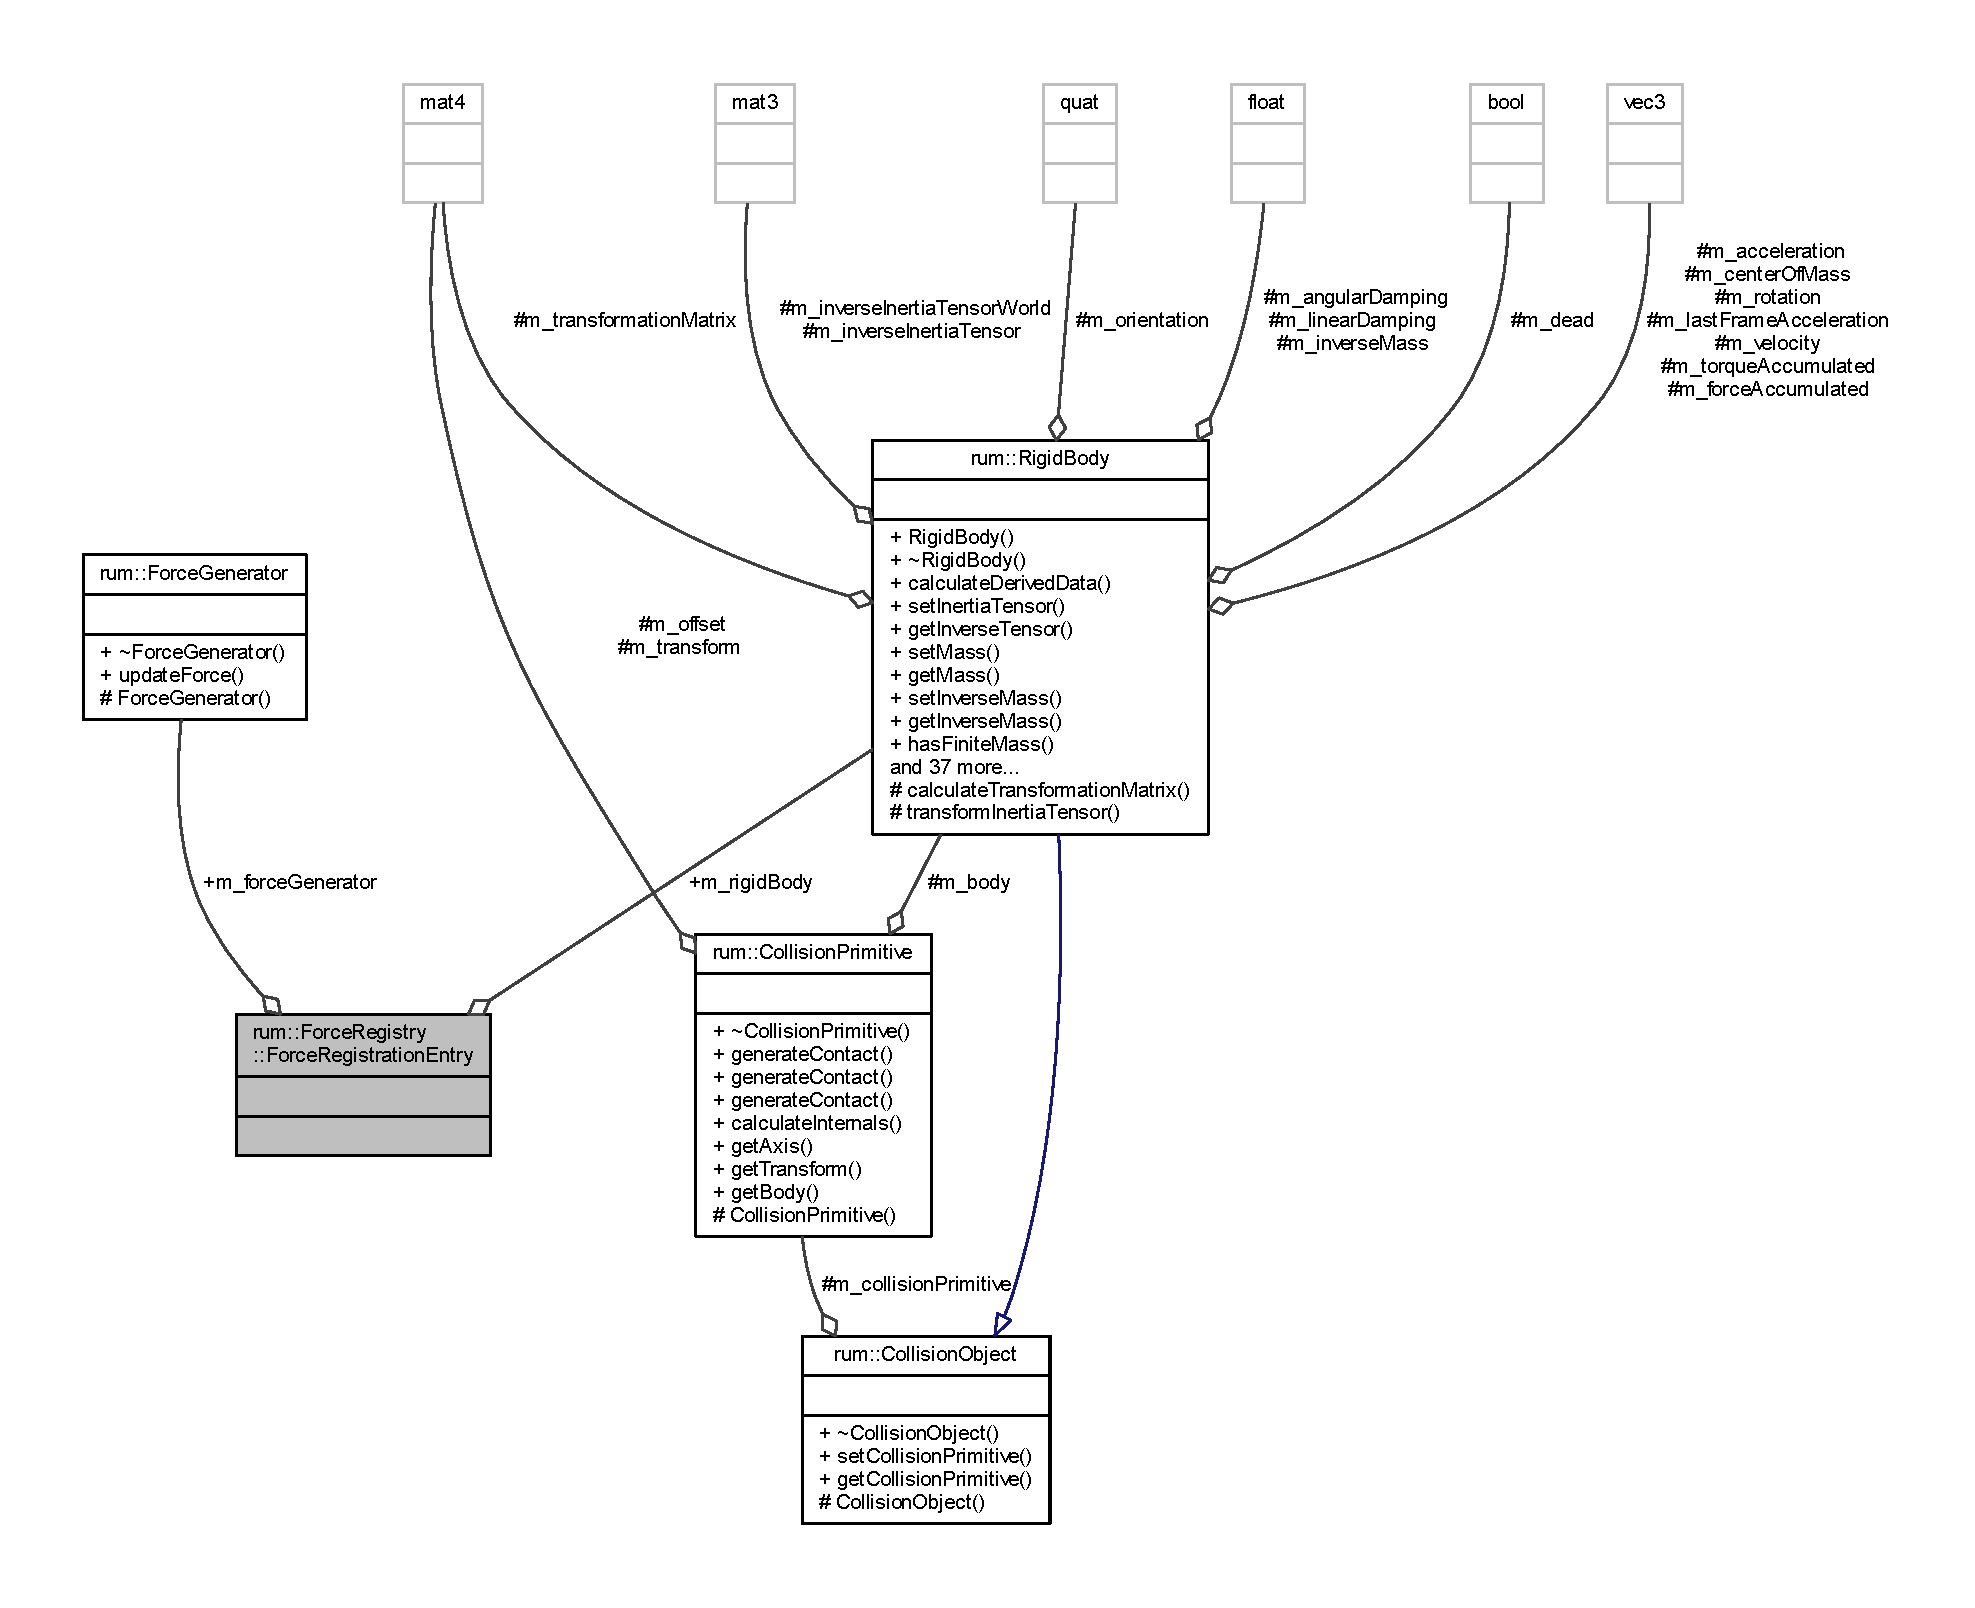
\includegraphics[width=350pt]{structrum_1_1_force_registry_1_1_force_registration_entry__coll__graph}
\end{center}
\end{figure}
\subsection*{Public Attributes}
\begin{DoxyCompactItemize}
\item 
\hyperlink{classrum_1_1_rigid_body}{Rigid\+Body} $\ast$ \hyperlink{structrum_1_1_force_registry_1_1_force_registration_entry_a35ba48cd73a75a00b3f265517d598c60}{rigid\+Body}
\item 
\hyperlink{classrum_1_1_force_generator}{Force\+Generator} $\ast$ \hyperlink{structrum_1_1_force_registry_1_1_force_registration_entry_a869a20d3c38ba31167a2ddc29315c861}{force\+Generator}
\end{DoxyCompactItemize}


\subsection{Member Data Documentation}
\mbox{\Hypertarget{structrum_1_1_force_registry_1_1_force_registration_entry_a869a20d3c38ba31167a2ddc29315c861}\label{structrum_1_1_force_registry_1_1_force_registration_entry_a869a20d3c38ba31167a2ddc29315c861}} 
\index{rum\+::\+Force\+Registry\+::\+Force\+Registration\+Entry@{rum\+::\+Force\+Registry\+::\+Force\+Registration\+Entry}!force\+Generator@{force\+Generator}}
\index{force\+Generator@{force\+Generator}!rum\+::\+Force\+Registry\+::\+Force\+Registration\+Entry@{rum\+::\+Force\+Registry\+::\+Force\+Registration\+Entry}}
\subsubsection{\texorpdfstring{force\+Generator}{forceGenerator}}
{\footnotesize\ttfamily \hyperlink{classrum_1_1_force_generator}{Force\+Generator}$\ast$ rum\+::\+Force\+Registry\+::\+Force\+Registration\+Entry\+::force\+Generator}

\mbox{\Hypertarget{structrum_1_1_force_registry_1_1_force_registration_entry_a35ba48cd73a75a00b3f265517d598c60}\label{structrum_1_1_force_registry_1_1_force_registration_entry_a35ba48cd73a75a00b3f265517d598c60}} 
\index{rum\+::\+Force\+Registry\+::\+Force\+Registration\+Entry@{rum\+::\+Force\+Registry\+::\+Force\+Registration\+Entry}!rigid\+Body@{rigid\+Body}}
\index{rigid\+Body@{rigid\+Body}!rum\+::\+Force\+Registry\+::\+Force\+Registration\+Entry@{rum\+::\+Force\+Registry\+::\+Force\+Registration\+Entry}}
\subsubsection{\texorpdfstring{rigid\+Body}{rigidBody}}
{\footnotesize\ttfamily \hyperlink{classrum_1_1_rigid_body}{Rigid\+Body}$\ast$ rum\+::\+Force\+Registry\+::\+Force\+Registration\+Entry\+::rigid\+Body}



The documentation for this struct was generated from the following file\+:\begin{DoxyCompactItemize}
\item 
F\+:/\+Library/\+Documents/\+Job/\+Forschungsmaster/\+Rumble3\+D/\+Rumble3\+D/include/\+R3\+D/\+Rigid\+Body\+Engine/\hyperlink{_force_registry_8h}{Force\+Registry.\+h}\end{DoxyCompactItemize}

\hypertarget{classrum_1_1_force_registry}{}\section{rum\+:\+:Force\+Registry Class Reference}
\label{classrum_1_1_force_registry}\index{rum\+::\+Force\+Registry@{rum\+::\+Force\+Registry}}


{\ttfamily \#include $<$Force\+Registry.\+h$>$}



Collaboration diagram for rum\+:\+:Force\+Registry\+:\nopagebreak
\begin{figure}[H]
\begin{center}
\leavevmode
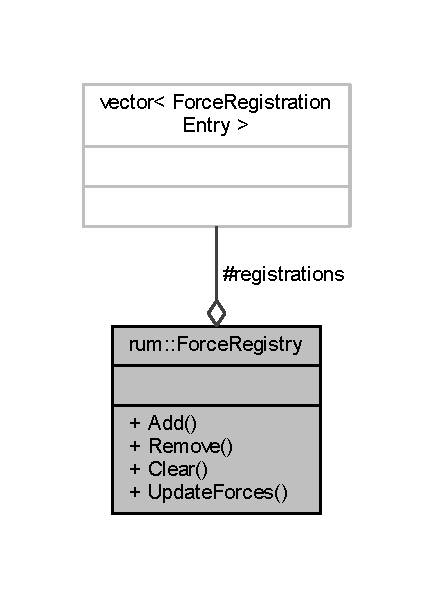
\includegraphics[width=208pt]{classrum_1_1_force_registry__coll__graph}
\end{center}
\end{figure}
\subsection*{Classes}
\begin{DoxyCompactItemize}
\item 
struct \hyperlink{structrum_1_1_force_registry_1_1_force_registration_entry}{Force\+Registration\+Entry}
\end{DoxyCompactItemize}
\subsection*{Public Member Functions}
\begin{DoxyCompactItemize}
\item 
void \hyperlink{classrum_1_1_force_registry_a3062f9ea0518bdef2624b39e17eb95d4}{Add} (\hyperlink{classrum_1_1_rigid_body}{Rigid\+Body} $\ast$rigid\+Body, \hyperlink{classrum_1_1_force_generator}{Force\+Generator} $\ast$fg)
\item 
void \hyperlink{classrum_1_1_force_registry_a26782e5d963910c3b61b27362591ba36}{Remove} (\hyperlink{classrum_1_1_rigid_body}{Rigid\+Body} $\ast$rigid\+Body, \hyperlink{classrum_1_1_force_generator}{Force\+Generator} $\ast$fg)
\item 
void \hyperlink{classrum_1_1_force_registry_a571da7ffd245ae2b09dd5538881a19de}{Clear} ()
\item 
void \hyperlink{classrum_1_1_force_registry_a162fdd23949e8c99523257a551c41e7c}{Update\+Forces} (\hyperlink{namespacerum_a7e8cca23573d5eaead0f138cbaa4862c}{real} duration)
\end{DoxyCompactItemize}
\subsection*{Protected Types}
\begin{DoxyCompactItemize}
\item 
typedef std\+::vector$<$ \hyperlink{structrum_1_1_force_registry_1_1_force_registration_entry}{Force\+Registration\+Entry} $>$ \hyperlink{classrum_1_1_force_registry_a9523605286e7ef4f693c3c485df757a6}{Registry}
\end{DoxyCompactItemize}
\subsection*{Protected Attributes}
\begin{DoxyCompactItemize}
\item 
\hyperlink{classrum_1_1_force_registry_a9523605286e7ef4f693c3c485df757a6}{Registry} \hyperlink{classrum_1_1_force_registry_a6b37ba6705d19a996324d1d10d642041}{registrations}
\end{DoxyCompactItemize}


\subsection{Member Typedef Documentation}
\mbox{\Hypertarget{classrum_1_1_force_registry_a9523605286e7ef4f693c3c485df757a6}\label{classrum_1_1_force_registry_a9523605286e7ef4f693c3c485df757a6}} 
\index{rum\+::\+Force\+Registry@{rum\+::\+Force\+Registry}!Registry@{Registry}}
\index{Registry@{Registry}!rum\+::\+Force\+Registry@{rum\+::\+Force\+Registry}}
\subsubsection{\texorpdfstring{Registry}{Registry}}
{\footnotesize\ttfamily typedef std\+::vector$<$\hyperlink{structrum_1_1_force_registry_1_1_force_registration_entry}{Force\+Registration\+Entry}$>$ \hyperlink{classrum_1_1_force_registry_a9523605286e7ef4f693c3c485df757a6}{rum\+::\+Force\+Registry\+::\+Registry}\hspace{0.3cm}{\ttfamily [protected]}}



\subsection{Member Function Documentation}
\mbox{\Hypertarget{classrum_1_1_force_registry_a3062f9ea0518bdef2624b39e17eb95d4}\label{classrum_1_1_force_registry_a3062f9ea0518bdef2624b39e17eb95d4}} 
\index{rum\+::\+Force\+Registry@{rum\+::\+Force\+Registry}!Add@{Add}}
\index{Add@{Add}!rum\+::\+Force\+Registry@{rum\+::\+Force\+Registry}}
\subsubsection{\texorpdfstring{Add()}{Add()}}
{\footnotesize\ttfamily void rum\+::\+Force\+Registry\+::\+Add (\begin{DoxyParamCaption}\item[{\hyperlink{classrum_1_1_rigid_body}{Rigid\+Body} $\ast$}]{rigid\+Body,  }\item[{\hyperlink{classrum_1_1_force_generator}{Force\+Generator} $\ast$}]{fg }\end{DoxyParamCaption})}

\mbox{\Hypertarget{classrum_1_1_force_registry_a571da7ffd245ae2b09dd5538881a19de}\label{classrum_1_1_force_registry_a571da7ffd245ae2b09dd5538881a19de}} 
\index{rum\+::\+Force\+Registry@{rum\+::\+Force\+Registry}!Clear@{Clear}}
\index{Clear@{Clear}!rum\+::\+Force\+Registry@{rum\+::\+Force\+Registry}}
\subsubsection{\texorpdfstring{Clear()}{Clear()}}
{\footnotesize\ttfamily void rum\+::\+Force\+Registry\+::\+Clear (\begin{DoxyParamCaption}{ }\end{DoxyParamCaption})}

\mbox{\Hypertarget{classrum_1_1_force_registry_a26782e5d963910c3b61b27362591ba36}\label{classrum_1_1_force_registry_a26782e5d963910c3b61b27362591ba36}} 
\index{rum\+::\+Force\+Registry@{rum\+::\+Force\+Registry}!Remove@{Remove}}
\index{Remove@{Remove}!rum\+::\+Force\+Registry@{rum\+::\+Force\+Registry}}
\subsubsection{\texorpdfstring{Remove()}{Remove()}}
{\footnotesize\ttfamily void rum\+::\+Force\+Registry\+::\+Remove (\begin{DoxyParamCaption}\item[{\hyperlink{classrum_1_1_rigid_body}{Rigid\+Body} $\ast$}]{rigid\+Body,  }\item[{\hyperlink{classrum_1_1_force_generator}{Force\+Generator} $\ast$}]{fg }\end{DoxyParamCaption})}

\mbox{\Hypertarget{classrum_1_1_force_registry_a162fdd23949e8c99523257a551c41e7c}\label{classrum_1_1_force_registry_a162fdd23949e8c99523257a551c41e7c}} 
\index{rum\+::\+Force\+Registry@{rum\+::\+Force\+Registry}!Update\+Forces@{Update\+Forces}}
\index{Update\+Forces@{Update\+Forces}!rum\+::\+Force\+Registry@{rum\+::\+Force\+Registry}}
\subsubsection{\texorpdfstring{Update\+Forces()}{UpdateForces()}}
{\footnotesize\ttfamily void rum\+::\+Force\+Registry\+::\+Update\+Forces (\begin{DoxyParamCaption}\item[{\hyperlink{namespacerum_a7e8cca23573d5eaead0f138cbaa4862c}{real}}]{duration }\end{DoxyParamCaption})}



\subsection{Member Data Documentation}
\mbox{\Hypertarget{classrum_1_1_force_registry_a6b37ba6705d19a996324d1d10d642041}\label{classrum_1_1_force_registry_a6b37ba6705d19a996324d1d10d642041}} 
\index{rum\+::\+Force\+Registry@{rum\+::\+Force\+Registry}!registrations@{registrations}}
\index{registrations@{registrations}!rum\+::\+Force\+Registry@{rum\+::\+Force\+Registry}}
\subsubsection{\texorpdfstring{registrations}{registrations}}
{\footnotesize\ttfamily \hyperlink{classrum_1_1_force_registry_a9523605286e7ef4f693c3c485df757a6}{Registry} rum\+::\+Force\+Registry\+::registrations\hspace{0.3cm}{\ttfamily [protected]}}



The documentation for this class was generated from the following files\+:\begin{DoxyCompactItemize}
\item 
F\+:/\+Library/\+Documents/\+Job/\+Forschungsmaster/\+Rumble3\+D/\+Rumble3\+D/include/\+R3\+D/\+Rigid\+Body\+Engine/\hyperlink{_force_registry_8h}{Force\+Registry.\+h}\item 
F\+:/\+Library/\+Documents/\+Job/\+Forschungsmaster/\+Rumble3\+D/\+Rumble3\+D/src/\+Rigid\+Body\+Engine/\hyperlink{_force_registry_8cpp}{Force\+Registry.\+cpp}\end{DoxyCompactItemize}

\hypertarget{classrum_1_1_gravity}{}\section{rum\+:\+:Gravity Class Reference}
\label{classrum_1_1_gravity}\index{rum\+::\+Gravity@{rum\+::\+Gravity}}


{\ttfamily \#include $<$Gravity.\+h$>$}



Inheritance diagram for rum\+:\+:Gravity\+:\nopagebreak
\begin{figure}[H]
\begin{center}
\leavevmode
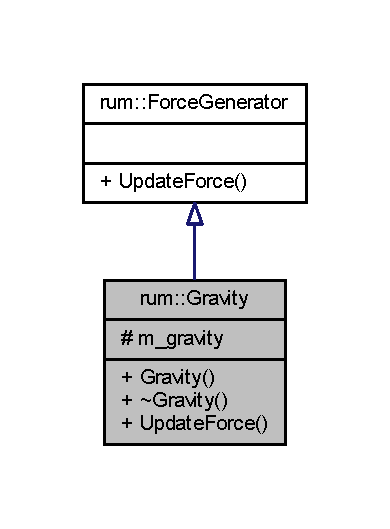
\includegraphics[width=187pt]{classrum_1_1_gravity__inherit__graph}
\end{center}
\end{figure}


Collaboration diagram for rum\+:\+:Gravity\+:\nopagebreak
\begin{figure}[H]
\begin{center}
\leavevmode
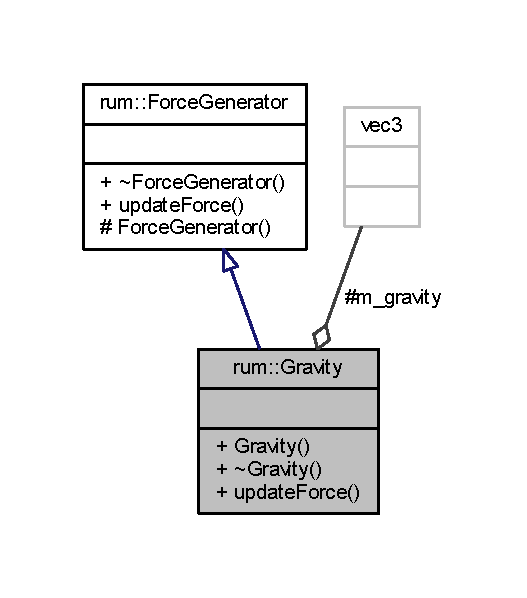
\includegraphics[width=256pt]{classrum_1_1_gravity__coll__graph}
\end{center}
\end{figure}
\subsection*{Public Member Functions}
\begin{DoxyCompactItemize}
\item 
\hyperlink{classrum_1_1_gravity_a9fca05b6d906fec4c40507b0c738dff8}{Gravity} (const glm\+::vec3 \&gravity)
\item 
\hyperlink{classrum_1_1_gravity_a67fc63876df40007e8c7bde5e8a72569}{$\sim$\+Gravity} ()
\item 
virtual void \hyperlink{classrum_1_1_gravity_a721c721904536378636143b21486ea2c}{Update\+Force} (\hyperlink{classrum_1_1_rigid_body}{Rigid\+Body} $\ast$body, \hyperlink{namespacerum_a7e8cca23573d5eaead0f138cbaa4862c}{real} duration) override
\end{DoxyCompactItemize}
\subsection*{Protected Attributes}
\begin{DoxyCompactItemize}
\item 
glm\+::vec3 \hyperlink{classrum_1_1_gravity_a82c9f64363024c45e96ba851a612613b}{m\+\_\+gravity}
\end{DoxyCompactItemize}


\subsection{Constructor \& Destructor Documentation}
\mbox{\Hypertarget{classrum_1_1_gravity_a9fca05b6d906fec4c40507b0c738dff8}\label{classrum_1_1_gravity_a9fca05b6d906fec4c40507b0c738dff8}} 
\index{rum\+::\+Gravity@{rum\+::\+Gravity}!Gravity@{Gravity}}
\index{Gravity@{Gravity}!rum\+::\+Gravity@{rum\+::\+Gravity}}
\subsubsection{\texorpdfstring{Gravity()}{Gravity()}}
{\footnotesize\ttfamily rum\+::\+Gravity\+::\+Gravity (\begin{DoxyParamCaption}\item[{const glm\+::vec3 \&}]{gravity }\end{DoxyParamCaption})}

\mbox{\Hypertarget{classrum_1_1_gravity_a67fc63876df40007e8c7bde5e8a72569}\label{classrum_1_1_gravity_a67fc63876df40007e8c7bde5e8a72569}} 
\index{rum\+::\+Gravity@{rum\+::\+Gravity}!````~Gravity@{$\sim$\+Gravity}}
\index{````~Gravity@{$\sim$\+Gravity}!rum\+::\+Gravity@{rum\+::\+Gravity}}
\subsubsection{\texorpdfstring{$\sim$\+Gravity()}{~Gravity()}}
{\footnotesize\ttfamily rum\+::\+Gravity\+::$\sim$\+Gravity (\begin{DoxyParamCaption}{ }\end{DoxyParamCaption})}



\subsection{Member Function Documentation}
\mbox{\Hypertarget{classrum_1_1_gravity_a721c721904536378636143b21486ea2c}\label{classrum_1_1_gravity_a721c721904536378636143b21486ea2c}} 
\index{rum\+::\+Gravity@{rum\+::\+Gravity}!Update\+Force@{Update\+Force}}
\index{Update\+Force@{Update\+Force}!rum\+::\+Gravity@{rum\+::\+Gravity}}
\subsubsection{\texorpdfstring{Update\+Force()}{UpdateForce()}}
{\footnotesize\ttfamily void rum\+::\+Gravity\+::\+Update\+Force (\begin{DoxyParamCaption}\item[{\hyperlink{classrum_1_1_rigid_body}{Rigid\+Body} $\ast$}]{body,  }\item[{\hyperlink{namespacerum_a7e8cca23573d5eaead0f138cbaa4862c}{real}}]{duration }\end{DoxyParamCaption})\hspace{0.3cm}{\ttfamily [override]}, {\ttfamily [virtual]}}



Implements \hyperlink{classrum_1_1_force_generator_a6b038c9a39e4cf64b2dcf2741804a824}{rum\+::\+Force\+Generator}.



\subsection{Member Data Documentation}
\mbox{\Hypertarget{classrum_1_1_gravity_a82c9f64363024c45e96ba851a612613b}\label{classrum_1_1_gravity_a82c9f64363024c45e96ba851a612613b}} 
\index{rum\+::\+Gravity@{rum\+::\+Gravity}!m\+\_\+gravity@{m\+\_\+gravity}}
\index{m\+\_\+gravity@{m\+\_\+gravity}!rum\+::\+Gravity@{rum\+::\+Gravity}}
\subsubsection{\texorpdfstring{m\+\_\+gravity}{m\_gravity}}
{\footnotesize\ttfamily glm\+::vec3 rum\+::\+Gravity\+::m\+\_\+gravity\hspace{0.3cm}{\ttfamily [protected]}}



The documentation for this class was generated from the following files\+:\begin{DoxyCompactItemize}
\item 
F\+:/\+Library/\+Documents/\+Job/\+Forschungsmaster/\+Rumble3\+D/\+Rumble3\+D/include/\+R3\+D/\+Rigid\+Body\+Engine/\hyperlink{_gravity_8h}{Gravity.\+h}\item 
F\+:/\+Library/\+Documents/\+Job/\+Forschungsmaster/\+Rumble3\+D/\+Rumble3\+D/src/\+Rigid\+Body\+Engine/\hyperlink{_gravity_8cpp}{Gravity.\+cpp}\end{DoxyCompactItemize}

\hypertarget{classrum_1_1_particle}{}\section{rum\+:\+:Particle Class Reference}
\label{classrum_1_1_particle}\index{rum\+::\+Particle@{rum\+::\+Particle}}


{\ttfamily \#include $<$Particle.\+h$>$}



Collaboration diagram for rum\+:\+:Particle\+:\nopagebreak
\begin{figure}[H]
\begin{center}
\leavevmode
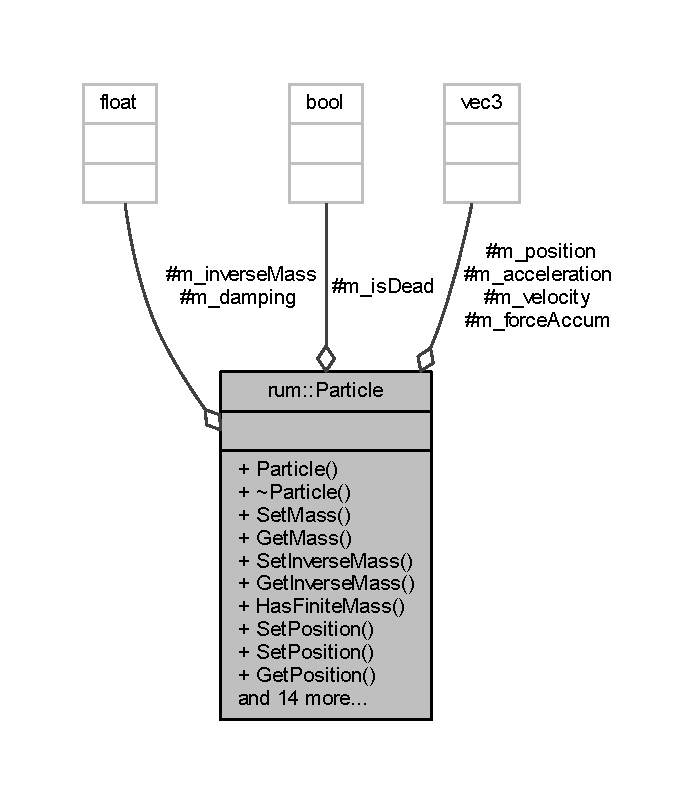
\includegraphics[width=335pt]{classrum_1_1_particle__coll__graph}
\end{center}
\end{figure}
\subsection*{Public Member Functions}
\begin{DoxyCompactItemize}
\item 
\hyperlink{classrum_1_1_particle_a9ae5ce0fc18a8be75950b336b92ecd75}{Particle} ()
\item 
virtual \hyperlink{classrum_1_1_particle_abc143197fe05fa60a1a3ccbf7b5f0fe8}{$\sim$\+Particle} ()
\item 
void \hyperlink{classrum_1_1_particle_a6525cbbbf7709bdacb7cb431d3622661}{Set\+Mass} (const \hyperlink{namespacerum_a7e8cca23573d5eaead0f138cbaa4862c}{real} mass)
\item 
\hyperlink{namespacerum_a7e8cca23573d5eaead0f138cbaa4862c}{real} \hyperlink{classrum_1_1_particle_a060c6f1db7424d67b4c01e6f7e538eca}{Get\+Mass} () const
\item 
void \hyperlink{classrum_1_1_particle_a2233ab971870fc1cf2337f01cdcae4fb}{Set\+Inverse\+Mass} (const \hyperlink{namespacerum_a7e8cca23573d5eaead0f138cbaa4862c}{real} inverse\+Mass)
\item 
\hyperlink{namespacerum_a7e8cca23573d5eaead0f138cbaa4862c}{real} \hyperlink{classrum_1_1_particle_a97e3662e7232daf4f2eabb79e4e06a3e}{Get\+Inverse\+Mass} () const
\item 
bool \hyperlink{classrum_1_1_particle_a0c19cd4e0c2933b4cc6357bb70c2c1a1}{Has\+Finite\+Mass} ()
\item 
void \hyperlink{classrum_1_1_particle_a2c564f2fe0122a6dd33b8113fde29e6d}{Set\+Position} (const glm\+::vec3 \&position)
\item 
void \hyperlink{classrum_1_1_particle_a1886668419cd31d6e0dacd1b62087ca0}{Set\+Position} (const \hyperlink{namespacerum_a7e8cca23573d5eaead0f138cbaa4862c}{real} x, const \hyperlink{namespacerum_a7e8cca23573d5eaead0f138cbaa4862c}{real} y, const \hyperlink{namespacerum_a7e8cca23573d5eaead0f138cbaa4862c}{real} z)
\item 
const glm\+::vec3 \& \hyperlink{classrum_1_1_particle_a78064d4405febbf7939070d1d2861594}{Get\+Position} () const
\item 
void \hyperlink{classrum_1_1_particle_a48c69c70728f76190cf698a0bb733607}{Set\+Velocity} (const glm\+::vec3 \&velocity)
\item 
void \hyperlink{classrum_1_1_particle_a481befad17e369f9ca7de3d60965a5d8}{Set\+Velocity} (const \hyperlink{namespacerum_a7e8cca23573d5eaead0f138cbaa4862c}{real} x, const \hyperlink{namespacerum_a7e8cca23573d5eaead0f138cbaa4862c}{real} y, const \hyperlink{namespacerum_a7e8cca23573d5eaead0f138cbaa4862c}{real} z)
\item 
const glm\+::vec3 \& \hyperlink{classrum_1_1_particle_adc199154d918e360103fa99f5b697604}{Get\+Velocity} () const
\item 
void \hyperlink{classrum_1_1_particle_a541556744b743995687bfabd42be67eb}{Set\+Acceleration} (const glm\+::vec3 \&acceleration)
\item 
void \hyperlink{classrum_1_1_particle_abfc528b024698e69b09b33ca6828f551}{Set\+Acceleration} (const \hyperlink{namespacerum_a7e8cca23573d5eaead0f138cbaa4862c}{real} x, const \hyperlink{namespacerum_a7e8cca23573d5eaead0f138cbaa4862c}{real} y, const \hyperlink{namespacerum_a7e8cca23573d5eaead0f138cbaa4862c}{real} z)
\item 
const glm\+::vec3 \& \hyperlink{classrum_1_1_particle_a2fee14e654f4914de9c5455d26223b86}{Get\+Acceleration} () const
\item 
void \hyperlink{classrum_1_1_particle_a9472726d229860f267dc8b7e8b7fe2cc}{Set\+Damping} (const \hyperlink{namespacerum_a7e8cca23573d5eaead0f138cbaa4862c}{real} damping)
\item 
\hyperlink{namespacerum_a7e8cca23573d5eaead0f138cbaa4862c}{real} \hyperlink{classrum_1_1_particle_a8635e9e5ab669d9d754195a265293dde}{Get\+Damping} () const
\item 
void \hyperlink{classrum_1_1_particle_acd315e7907736b20493e091651cff616}{Set\+Is\+Dead} (bool is\+Dead)
\item 
bool \hyperlink{classrum_1_1_particle_af9cc5e4971981a3ad4c59370aa80a6ee}{Is\+Dead} ()
\item 
const glm\+::vec3 \& \hyperlink{classrum_1_1_particle_aa13821d1abbcc67a90d37936b58c632b}{Get\+Force\+Accum} ()
\item 
void \hyperlink{classrum_1_1_particle_adb76d2210f9fc1f95839a3c116a52b38}{Clear\+Accumulator} ()
\item 
void \hyperlink{classrum_1_1_particle_afe6a59e7c46860227b61b57eee5a37b0}{Add\+Force} (const glm\+::vec3 \&force)
\item 
virtual void \hyperlink{classrum_1_1_particle_ac2200e991b81a380177275d6dd04ab64}{Integrate} (\hyperlink{namespacerum_a7e8cca23573d5eaead0f138cbaa4862c}{real} duration)
\end{DoxyCompactItemize}
\subsection*{Protected Attributes}
\begin{DoxyCompactItemize}
\item 
glm\+::vec3 \hyperlink{classrum_1_1_particle_a6e7c397b620c9d03fb6c7d4359649d40}{m\+\_\+position}
\item 
glm\+::vec3 \hyperlink{classrum_1_1_particle_a8dfab481a4ef728d40e86f7369baf307}{m\+\_\+velocity}
\item 
glm\+::vec3 \hyperlink{classrum_1_1_particle_aee85fab3a2d274ecc7d997f1c0c34132}{m\+\_\+acceleration}
\item 
glm\+::vec3 \hyperlink{classrum_1_1_particle_afe25996db7b8665b775e4b46d52fea50}{m\+\_\+force\+Accum}
\item 
\hyperlink{namespacerum_a7e8cca23573d5eaead0f138cbaa4862c}{real} \hyperlink{classrum_1_1_particle_a7fa92aadbccc9d999d84cef129cf8870}{m\+\_\+inverse\+Mass}
\item 
\hyperlink{namespacerum_a7e8cca23573d5eaead0f138cbaa4862c}{real} \hyperlink{classrum_1_1_particle_a76f5e4b0ed29a1d86419230621dd1047}{m\+\_\+damping}
\item 
bool \hyperlink{classrum_1_1_particle_ab056fc8b2187694c0742bd234b9cc6a3}{m\+\_\+is\+Dead}
\end{DoxyCompactItemize}


\subsection{Constructor \& Destructor Documentation}
\mbox{\Hypertarget{classrum_1_1_particle_a9ae5ce0fc18a8be75950b336b92ecd75}\label{classrum_1_1_particle_a9ae5ce0fc18a8be75950b336b92ecd75}} 
\index{rum\+::\+Particle@{rum\+::\+Particle}!Particle@{Particle}}
\index{Particle@{Particle}!rum\+::\+Particle@{rum\+::\+Particle}}
\subsubsection{\texorpdfstring{Particle()}{Particle()}}
{\footnotesize\ttfamily rum\+::\+Particle\+::\+Particle (\begin{DoxyParamCaption}{ }\end{DoxyParamCaption})\hspace{0.3cm}{\ttfamily [explicit]}}

\mbox{\Hypertarget{classrum_1_1_particle_abc143197fe05fa60a1a3ccbf7b5f0fe8}\label{classrum_1_1_particle_abc143197fe05fa60a1a3ccbf7b5f0fe8}} 
\index{rum\+::\+Particle@{rum\+::\+Particle}!````~Particle@{$\sim$\+Particle}}
\index{````~Particle@{$\sim$\+Particle}!rum\+::\+Particle@{rum\+::\+Particle}}
\subsubsection{\texorpdfstring{$\sim$\+Particle()}{~Particle()}}
{\footnotesize\ttfamily rum\+::\+Particle\+::$\sim$\+Particle (\begin{DoxyParamCaption}{ }\end{DoxyParamCaption})\hspace{0.3cm}{\ttfamily [virtual]}}



\subsection{Member Function Documentation}
\mbox{\Hypertarget{classrum_1_1_particle_afe6a59e7c46860227b61b57eee5a37b0}\label{classrum_1_1_particle_afe6a59e7c46860227b61b57eee5a37b0}} 
\index{rum\+::\+Particle@{rum\+::\+Particle}!Add\+Force@{Add\+Force}}
\index{Add\+Force@{Add\+Force}!rum\+::\+Particle@{rum\+::\+Particle}}
\subsubsection{\texorpdfstring{Add\+Force()}{AddForce()}}
{\footnotesize\ttfamily void rum\+::\+Particle\+::\+Add\+Force (\begin{DoxyParamCaption}\item[{const glm\+::vec3 \&}]{force }\end{DoxyParamCaption})}

Add a force to the force accumulator. \mbox{\Hypertarget{classrum_1_1_particle_adb76d2210f9fc1f95839a3c116a52b38}\label{classrum_1_1_particle_adb76d2210f9fc1f95839a3c116a52b38}} 
\index{rum\+::\+Particle@{rum\+::\+Particle}!Clear\+Accumulator@{Clear\+Accumulator}}
\index{Clear\+Accumulator@{Clear\+Accumulator}!rum\+::\+Particle@{rum\+::\+Particle}}
\subsubsection{\texorpdfstring{Clear\+Accumulator()}{ClearAccumulator()}}
{\footnotesize\ttfamily void rum\+::\+Particle\+::\+Clear\+Accumulator (\begin{DoxyParamCaption}{ }\end{DoxyParamCaption})}

Set the accumulated forces to zero. \mbox{\Hypertarget{classrum_1_1_particle_a2fee14e654f4914de9c5455d26223b86}\label{classrum_1_1_particle_a2fee14e654f4914de9c5455d26223b86}} 
\index{rum\+::\+Particle@{rum\+::\+Particle}!Get\+Acceleration@{Get\+Acceleration}}
\index{Get\+Acceleration@{Get\+Acceleration}!rum\+::\+Particle@{rum\+::\+Particle}}
\subsubsection{\texorpdfstring{Get\+Acceleration()}{GetAcceleration()}}
{\footnotesize\ttfamily const glm\+::vec3 \& rum\+::\+Particle\+::\+Get\+Acceleration (\begin{DoxyParamCaption}{ }\end{DoxyParamCaption}) const}

\mbox{\Hypertarget{classrum_1_1_particle_a8635e9e5ab669d9d754195a265293dde}\label{classrum_1_1_particle_a8635e9e5ab669d9d754195a265293dde}} 
\index{rum\+::\+Particle@{rum\+::\+Particle}!Get\+Damping@{Get\+Damping}}
\index{Get\+Damping@{Get\+Damping}!rum\+::\+Particle@{rum\+::\+Particle}}
\subsubsection{\texorpdfstring{Get\+Damping()}{GetDamping()}}
{\footnotesize\ttfamily \hyperlink{namespacerum_a7e8cca23573d5eaead0f138cbaa4862c}{real} rum\+::\+Particle\+::\+Get\+Damping (\begin{DoxyParamCaption}{ }\end{DoxyParamCaption}) const}

Get the linear damping constant of this particle. \mbox{\Hypertarget{classrum_1_1_particle_aa13821d1abbcc67a90d37936b58c632b}\label{classrum_1_1_particle_aa13821d1abbcc67a90d37936b58c632b}} 
\index{rum\+::\+Particle@{rum\+::\+Particle}!Get\+Force\+Accum@{Get\+Force\+Accum}}
\index{Get\+Force\+Accum@{Get\+Force\+Accum}!rum\+::\+Particle@{rum\+::\+Particle}}
\subsubsection{\texorpdfstring{Get\+Force\+Accum()}{GetForceAccum()}}
{\footnotesize\ttfamily const glm\+::vec3 \& rum\+::\+Particle\+::\+Get\+Force\+Accum (\begin{DoxyParamCaption}{ }\end{DoxyParamCaption})}

Get current sum of accumulated forces. \mbox{\Hypertarget{classrum_1_1_particle_a97e3662e7232daf4f2eabb79e4e06a3e}\label{classrum_1_1_particle_a97e3662e7232daf4f2eabb79e4e06a3e}} 
\index{rum\+::\+Particle@{rum\+::\+Particle}!Get\+Inverse\+Mass@{Get\+Inverse\+Mass}}
\index{Get\+Inverse\+Mass@{Get\+Inverse\+Mass}!rum\+::\+Particle@{rum\+::\+Particle}}
\subsubsection{\texorpdfstring{Get\+Inverse\+Mass()}{GetInverseMass()}}
{\footnotesize\ttfamily \hyperlink{namespacerum_a7e8cca23573d5eaead0f138cbaa4862c}{real} rum\+::\+Particle\+::\+Get\+Inverse\+Mass (\begin{DoxyParamCaption}{ }\end{DoxyParamCaption}) const}

Get the current inverse mass of this particle If particle has infinite mass, inverse mass will be 0. \mbox{\Hypertarget{classrum_1_1_particle_a060c6f1db7424d67b4c01e6f7e538eca}\label{classrum_1_1_particle_a060c6f1db7424d67b4c01e6f7e538eca}} 
\index{rum\+::\+Particle@{rum\+::\+Particle}!Get\+Mass@{Get\+Mass}}
\index{Get\+Mass@{Get\+Mass}!rum\+::\+Particle@{rum\+::\+Particle}}
\subsubsection{\texorpdfstring{Get\+Mass()}{GetMass()}}
{\footnotesize\ttfamily \hyperlink{namespacerum_a7e8cca23573d5eaead0f138cbaa4862c}{real} rum\+::\+Particle\+::\+Get\+Mass (\begin{DoxyParamCaption}{ }\end{DoxyParamCaption}) const}

Get the current mass of this particle. \mbox{\Hypertarget{classrum_1_1_particle_a78064d4405febbf7939070d1d2861594}\label{classrum_1_1_particle_a78064d4405febbf7939070d1d2861594}} 
\index{rum\+::\+Particle@{rum\+::\+Particle}!Get\+Position@{Get\+Position}}
\index{Get\+Position@{Get\+Position}!rum\+::\+Particle@{rum\+::\+Particle}}
\subsubsection{\texorpdfstring{Get\+Position()}{GetPosition()}}
{\footnotesize\ttfamily const glm\+::vec3 \& rum\+::\+Particle\+::\+Get\+Position (\begin{DoxyParamCaption}{ }\end{DoxyParamCaption}) const}

Get the current position of this particle. \mbox{\Hypertarget{classrum_1_1_particle_adc199154d918e360103fa99f5b697604}\label{classrum_1_1_particle_adc199154d918e360103fa99f5b697604}} 
\index{rum\+::\+Particle@{rum\+::\+Particle}!Get\+Velocity@{Get\+Velocity}}
\index{Get\+Velocity@{Get\+Velocity}!rum\+::\+Particle@{rum\+::\+Particle}}
\subsubsection{\texorpdfstring{Get\+Velocity()}{GetVelocity()}}
{\footnotesize\ttfamily const glm\+::vec3 \& rum\+::\+Particle\+::\+Get\+Velocity (\begin{DoxyParamCaption}{ }\end{DoxyParamCaption}) const}

Get the current velocity of this particle. \mbox{\Hypertarget{classrum_1_1_particle_a0c19cd4e0c2933b4cc6357bb70c2c1a1}\label{classrum_1_1_particle_a0c19cd4e0c2933b4cc6357bb70c2c1a1}} 
\index{rum\+::\+Particle@{rum\+::\+Particle}!Has\+Finite\+Mass@{Has\+Finite\+Mass}}
\index{Has\+Finite\+Mass@{Has\+Finite\+Mass}!rum\+::\+Particle@{rum\+::\+Particle}}
\subsubsection{\texorpdfstring{Has\+Finite\+Mass()}{HasFiniteMass()}}
{\footnotesize\ttfamily bool rum\+::\+Particle\+::\+Has\+Finite\+Mass (\begin{DoxyParamCaption}{ }\end{DoxyParamCaption})}

Check if this particle has infinite mass. \begin{DoxyReturn}{Returns}
True if mass is infinite. 
\end{DoxyReturn}
\mbox{\Hypertarget{classrum_1_1_particle_ac2200e991b81a380177275d6dd04ab64}\label{classrum_1_1_particle_ac2200e991b81a380177275d6dd04ab64}} 
\index{rum\+::\+Particle@{rum\+::\+Particle}!Integrate@{Integrate}}
\index{Integrate@{Integrate}!rum\+::\+Particle@{rum\+::\+Particle}}
\subsubsection{\texorpdfstring{Integrate()}{Integrate()}}
{\footnotesize\ttfamily void rum\+::\+Particle\+::\+Integrate (\begin{DoxyParamCaption}\item[{\hyperlink{namespacerum_a7e8cca23573d5eaead0f138cbaa4862c}{real}}]{duration }\end{DoxyParamCaption})\hspace{0.3cm}{\ttfamily [virtual]}}

Apply forces and update position, velocity and acceleration. \mbox{\Hypertarget{classrum_1_1_particle_af9cc5e4971981a3ad4c59370aa80a6ee}\label{classrum_1_1_particle_af9cc5e4971981a3ad4c59370aa80a6ee}} 
\index{rum\+::\+Particle@{rum\+::\+Particle}!Is\+Dead@{Is\+Dead}}
\index{Is\+Dead@{Is\+Dead}!rum\+::\+Particle@{rum\+::\+Particle}}
\subsubsection{\texorpdfstring{Is\+Dead()}{IsDead()}}
{\footnotesize\ttfamily bool rum\+::\+Particle\+::\+Is\+Dead (\begin{DoxyParamCaption}{ }\end{DoxyParamCaption})}

Check if this particle is dead. \mbox{\Hypertarget{classrum_1_1_particle_a541556744b743995687bfabd42be67eb}\label{classrum_1_1_particle_a541556744b743995687bfabd42be67eb}} 
\index{rum\+::\+Particle@{rum\+::\+Particle}!Set\+Acceleration@{Set\+Acceleration}}
\index{Set\+Acceleration@{Set\+Acceleration}!rum\+::\+Particle@{rum\+::\+Particle}}
\subsubsection{\texorpdfstring{Set\+Acceleration()}{SetAcceleration()}\hspace{0.1cm}{\footnotesize\ttfamily [1/2]}}
{\footnotesize\ttfamily void rum\+::\+Particle\+::\+Set\+Acceleration (\begin{DoxyParamCaption}\item[{const glm\+::vec3 \&}]{acceleration }\end{DoxyParamCaption})}

\mbox{\Hypertarget{classrum_1_1_particle_abfc528b024698e69b09b33ca6828f551}\label{classrum_1_1_particle_abfc528b024698e69b09b33ca6828f551}} 
\index{rum\+::\+Particle@{rum\+::\+Particle}!Set\+Acceleration@{Set\+Acceleration}}
\index{Set\+Acceleration@{Set\+Acceleration}!rum\+::\+Particle@{rum\+::\+Particle}}
\subsubsection{\texorpdfstring{Set\+Acceleration()}{SetAcceleration()}\hspace{0.1cm}{\footnotesize\ttfamily [2/2]}}
{\footnotesize\ttfamily void rum\+::\+Particle\+::\+Set\+Acceleration (\begin{DoxyParamCaption}\item[{const \hyperlink{namespacerum_a7e8cca23573d5eaead0f138cbaa4862c}{real}}]{x,  }\item[{const \hyperlink{namespacerum_a7e8cca23573d5eaead0f138cbaa4862c}{real}}]{y,  }\item[{const \hyperlink{namespacerum_a7e8cca23573d5eaead0f138cbaa4862c}{real}}]{z }\end{DoxyParamCaption})}

\mbox{\Hypertarget{classrum_1_1_particle_a9472726d229860f267dc8b7e8b7fe2cc}\label{classrum_1_1_particle_a9472726d229860f267dc8b7e8b7fe2cc}} 
\index{rum\+::\+Particle@{rum\+::\+Particle}!Set\+Damping@{Set\+Damping}}
\index{Set\+Damping@{Set\+Damping}!rum\+::\+Particle@{rum\+::\+Particle}}
\subsubsection{\texorpdfstring{Set\+Damping()}{SetDamping()}}
{\footnotesize\ttfamily void rum\+::\+Particle\+::\+Set\+Damping (\begin{DoxyParamCaption}\item[{const \hyperlink{namespacerum_a7e8cca23573d5eaead0f138cbaa4862c}{real}}]{damping }\end{DoxyParamCaption})}

Change the linear damping constant of this particle. \mbox{\Hypertarget{classrum_1_1_particle_a2233ab971870fc1cf2337f01cdcae4fb}\label{classrum_1_1_particle_a2233ab971870fc1cf2337f01cdcae4fb}} 
\index{rum\+::\+Particle@{rum\+::\+Particle}!Set\+Inverse\+Mass@{Set\+Inverse\+Mass}}
\index{Set\+Inverse\+Mass@{Set\+Inverse\+Mass}!rum\+::\+Particle@{rum\+::\+Particle}}
\subsubsection{\texorpdfstring{Set\+Inverse\+Mass()}{SetInverseMass()}}
{\footnotesize\ttfamily void rum\+::\+Particle\+::\+Set\+Inverse\+Mass (\begin{DoxyParamCaption}\item[{const \hyperlink{namespacerum_a7e8cca23573d5eaead0f138cbaa4862c}{real}}]{inverse\+Mass }\end{DoxyParamCaption})}

Change the inverse mass of this particle to the given value. Implicitly changes mass. 
\begin{DoxyParams}{Parameters}
{\em inverse\+Mass} & A value of 0 is equivalent to infinite mass. \\
\hline
\end{DoxyParams}
\mbox{\Hypertarget{classrum_1_1_particle_acd315e7907736b20493e091651cff616}\label{classrum_1_1_particle_acd315e7907736b20493e091651cff616}} 
\index{rum\+::\+Particle@{rum\+::\+Particle}!Set\+Is\+Dead@{Set\+Is\+Dead}}
\index{Set\+Is\+Dead@{Set\+Is\+Dead}!rum\+::\+Particle@{rum\+::\+Particle}}
\subsubsection{\texorpdfstring{Set\+Is\+Dead()}{SetIsDead()}}
{\footnotesize\ttfamily void rum\+::\+Particle\+::\+Set\+Is\+Dead (\begin{DoxyParamCaption}\item[{bool}]{is\+Dead }\end{DoxyParamCaption})}

Set dead state of this particle. \mbox{\Hypertarget{classrum_1_1_particle_a6525cbbbf7709bdacb7cb431d3622661}\label{classrum_1_1_particle_a6525cbbbf7709bdacb7cb431d3622661}} 
\index{rum\+::\+Particle@{rum\+::\+Particle}!Set\+Mass@{Set\+Mass}}
\index{Set\+Mass@{Set\+Mass}!rum\+::\+Particle@{rum\+::\+Particle}}
\subsubsection{\texorpdfstring{Set\+Mass()}{SetMass()}}
{\footnotesize\ttfamily void rum\+::\+Particle\+::\+Set\+Mass (\begin{DoxyParamCaption}\item[{const \hyperlink{namespacerum_a7e8cca23573d5eaead0f138cbaa4862c}{real}}]{mass }\end{DoxyParamCaption})}

Change the mass of this particle to the given given value. Implicitly changes inverse mass. \mbox{\Hypertarget{classrum_1_1_particle_a2c564f2fe0122a6dd33b8113fde29e6d}\label{classrum_1_1_particle_a2c564f2fe0122a6dd33b8113fde29e6d}} 
\index{rum\+::\+Particle@{rum\+::\+Particle}!Set\+Position@{Set\+Position}}
\index{Set\+Position@{Set\+Position}!rum\+::\+Particle@{rum\+::\+Particle}}
\subsubsection{\texorpdfstring{Set\+Position()}{SetPosition()}\hspace{0.1cm}{\footnotesize\ttfamily [1/2]}}
{\footnotesize\ttfamily void rum\+::\+Particle\+::\+Set\+Position (\begin{DoxyParamCaption}\item[{const glm\+::vec3 \&}]{position }\end{DoxyParamCaption})}

Change particle position to given vector. \mbox{\Hypertarget{classrum_1_1_particle_a1886668419cd31d6e0dacd1b62087ca0}\label{classrum_1_1_particle_a1886668419cd31d6e0dacd1b62087ca0}} 
\index{rum\+::\+Particle@{rum\+::\+Particle}!Set\+Position@{Set\+Position}}
\index{Set\+Position@{Set\+Position}!rum\+::\+Particle@{rum\+::\+Particle}}
\subsubsection{\texorpdfstring{Set\+Position()}{SetPosition()}\hspace{0.1cm}{\footnotesize\ttfamily [2/2]}}
{\footnotesize\ttfamily void rum\+::\+Particle\+::\+Set\+Position (\begin{DoxyParamCaption}\item[{const \hyperlink{namespacerum_a7e8cca23573d5eaead0f138cbaa4862c}{real}}]{x,  }\item[{const \hyperlink{namespacerum_a7e8cca23573d5eaead0f138cbaa4862c}{real}}]{y,  }\item[{const \hyperlink{namespacerum_a7e8cca23573d5eaead0f138cbaa4862c}{real}}]{z }\end{DoxyParamCaption})}

Change particle position to given coordinates. \mbox{\Hypertarget{classrum_1_1_particle_a48c69c70728f76190cf698a0bb733607}\label{classrum_1_1_particle_a48c69c70728f76190cf698a0bb733607}} 
\index{rum\+::\+Particle@{rum\+::\+Particle}!Set\+Velocity@{Set\+Velocity}}
\index{Set\+Velocity@{Set\+Velocity}!rum\+::\+Particle@{rum\+::\+Particle}}
\subsubsection{\texorpdfstring{Set\+Velocity()}{SetVelocity()}\hspace{0.1cm}{\footnotesize\ttfamily [1/2]}}
{\footnotesize\ttfamily void rum\+::\+Particle\+::\+Set\+Velocity (\begin{DoxyParamCaption}\item[{const glm\+::vec3 \&}]{velocity }\end{DoxyParamCaption})}

Change the current velocity of this particle to the given velocity. \mbox{\Hypertarget{classrum_1_1_particle_a481befad17e369f9ca7de3d60965a5d8}\label{classrum_1_1_particle_a481befad17e369f9ca7de3d60965a5d8}} 
\index{rum\+::\+Particle@{rum\+::\+Particle}!Set\+Velocity@{Set\+Velocity}}
\index{Set\+Velocity@{Set\+Velocity}!rum\+::\+Particle@{rum\+::\+Particle}}
\subsubsection{\texorpdfstring{Set\+Velocity()}{SetVelocity()}\hspace{0.1cm}{\footnotesize\ttfamily [2/2]}}
{\footnotesize\ttfamily void rum\+::\+Particle\+::\+Set\+Velocity (\begin{DoxyParamCaption}\item[{const \hyperlink{namespacerum_a7e8cca23573d5eaead0f138cbaa4862c}{real}}]{x,  }\item[{const \hyperlink{namespacerum_a7e8cca23573d5eaead0f138cbaa4862c}{real}}]{y,  }\item[{const \hyperlink{namespacerum_a7e8cca23573d5eaead0f138cbaa4862c}{real}}]{z }\end{DoxyParamCaption})}

Change the current velocity of this particle to the given velocity. 

\subsection{Member Data Documentation}
\mbox{\Hypertarget{classrum_1_1_particle_aee85fab3a2d274ecc7d997f1c0c34132}\label{classrum_1_1_particle_aee85fab3a2d274ecc7d997f1c0c34132}} 
\index{rum\+::\+Particle@{rum\+::\+Particle}!m\+\_\+acceleration@{m\+\_\+acceleration}}
\index{m\+\_\+acceleration@{m\+\_\+acceleration}!rum\+::\+Particle@{rum\+::\+Particle}}
\subsubsection{\texorpdfstring{m\+\_\+acceleration}{m\_acceleration}}
{\footnotesize\ttfamily glm\+::vec3 rum\+::\+Particle\+::m\+\_\+acceleration\hspace{0.3cm}{\ttfamily [protected]}}

\mbox{\Hypertarget{classrum_1_1_particle_a76f5e4b0ed29a1d86419230621dd1047}\label{classrum_1_1_particle_a76f5e4b0ed29a1d86419230621dd1047}} 
\index{rum\+::\+Particle@{rum\+::\+Particle}!m\+\_\+damping@{m\+\_\+damping}}
\index{m\+\_\+damping@{m\+\_\+damping}!rum\+::\+Particle@{rum\+::\+Particle}}
\subsubsection{\texorpdfstring{m\+\_\+damping}{m\_damping}}
{\footnotesize\ttfamily \hyperlink{namespacerum_a7e8cca23573d5eaead0f138cbaa4862c}{real} rum\+::\+Particle\+::m\+\_\+damping\hspace{0.3cm}{\ttfamily [protected]}}

\mbox{\Hypertarget{classrum_1_1_particle_afe25996db7b8665b775e4b46d52fea50}\label{classrum_1_1_particle_afe25996db7b8665b775e4b46d52fea50}} 
\index{rum\+::\+Particle@{rum\+::\+Particle}!m\+\_\+force\+Accum@{m\+\_\+force\+Accum}}
\index{m\+\_\+force\+Accum@{m\+\_\+force\+Accum}!rum\+::\+Particle@{rum\+::\+Particle}}
\subsubsection{\texorpdfstring{m\+\_\+force\+Accum}{m\_forceAccum}}
{\footnotesize\ttfamily glm\+::vec3 rum\+::\+Particle\+::m\+\_\+force\+Accum\hspace{0.3cm}{\ttfamily [protected]}}

\mbox{\Hypertarget{classrum_1_1_particle_a7fa92aadbccc9d999d84cef129cf8870}\label{classrum_1_1_particle_a7fa92aadbccc9d999d84cef129cf8870}} 
\index{rum\+::\+Particle@{rum\+::\+Particle}!m\+\_\+inverse\+Mass@{m\+\_\+inverse\+Mass}}
\index{m\+\_\+inverse\+Mass@{m\+\_\+inverse\+Mass}!rum\+::\+Particle@{rum\+::\+Particle}}
\subsubsection{\texorpdfstring{m\+\_\+inverse\+Mass}{m\_inverseMass}}
{\footnotesize\ttfamily \hyperlink{namespacerum_a7e8cca23573d5eaead0f138cbaa4862c}{real} rum\+::\+Particle\+::m\+\_\+inverse\+Mass\hspace{0.3cm}{\ttfamily [protected]}}

\mbox{\Hypertarget{classrum_1_1_particle_ab056fc8b2187694c0742bd234b9cc6a3}\label{classrum_1_1_particle_ab056fc8b2187694c0742bd234b9cc6a3}} 
\index{rum\+::\+Particle@{rum\+::\+Particle}!m\+\_\+is\+Dead@{m\+\_\+is\+Dead}}
\index{m\+\_\+is\+Dead@{m\+\_\+is\+Dead}!rum\+::\+Particle@{rum\+::\+Particle}}
\subsubsection{\texorpdfstring{m\+\_\+is\+Dead}{m\_isDead}}
{\footnotesize\ttfamily bool rum\+::\+Particle\+::m\+\_\+is\+Dead\hspace{0.3cm}{\ttfamily [protected]}}

\mbox{\Hypertarget{classrum_1_1_particle_a6e7c397b620c9d03fb6c7d4359649d40}\label{classrum_1_1_particle_a6e7c397b620c9d03fb6c7d4359649d40}} 
\index{rum\+::\+Particle@{rum\+::\+Particle}!m\+\_\+position@{m\+\_\+position}}
\index{m\+\_\+position@{m\+\_\+position}!rum\+::\+Particle@{rum\+::\+Particle}}
\subsubsection{\texorpdfstring{m\+\_\+position}{m\_position}}
{\footnotesize\ttfamily glm\+::vec3 rum\+::\+Particle\+::m\+\_\+position\hspace{0.3cm}{\ttfamily [protected]}}

\mbox{\Hypertarget{classrum_1_1_particle_a8dfab481a4ef728d40e86f7369baf307}\label{classrum_1_1_particle_a8dfab481a4ef728d40e86f7369baf307}} 
\index{rum\+::\+Particle@{rum\+::\+Particle}!m\+\_\+velocity@{m\+\_\+velocity}}
\index{m\+\_\+velocity@{m\+\_\+velocity}!rum\+::\+Particle@{rum\+::\+Particle}}
\subsubsection{\texorpdfstring{m\+\_\+velocity}{m\_velocity}}
{\footnotesize\ttfamily glm\+::vec3 rum\+::\+Particle\+::m\+\_\+velocity\hspace{0.3cm}{\ttfamily [protected]}}



The documentation for this class was generated from the following files\+:\begin{DoxyCompactItemize}
\item 
F\+:/\+Library/\+Documents/\+Job/\+Forschungsmaster/\+Rumble3\+D/\+Rumble3\+D/include/\+R3\+D/\+Particle\+Engine/\hyperlink{_particle_8h}{Particle.\+h}\item 
F\+:/\+Library/\+Documents/\+Job/\+Forschungsmaster/\+Rumble3\+D/\+Rumble3\+D/src/\+Particle\+Engine/\hyperlink{_particle_8cpp}{Particle.\+cpp}\end{DoxyCompactItemize}

\hypertarget{classrum_1_1_particle_anchored_spring}{}\section{rum\+:\+:Particle\+Anchored\+Spring Class Reference}
\label{classrum_1_1_particle_anchored_spring}\index{rum\+::\+Particle\+Anchored\+Spring@{rum\+::\+Particle\+Anchored\+Spring}}


{\ttfamily \#include $<$Particle\+Anchored\+Spring.\+h$>$}



Inheritance diagram for rum\+:\+:Particle\+Anchored\+Spring\+:\nopagebreak
\begin{figure}[H]
\begin{center}
\leavevmode
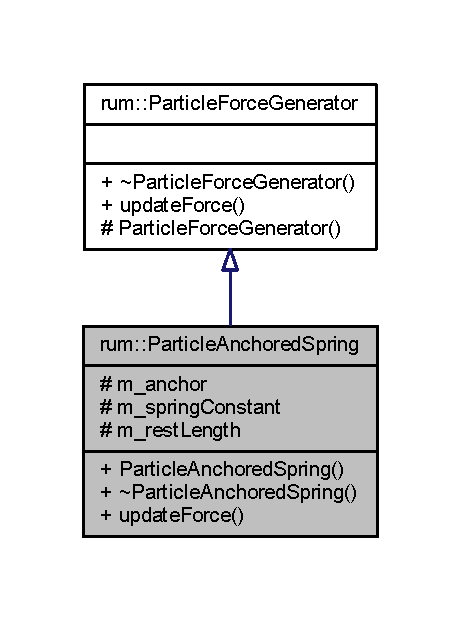
\includegraphics[width=221pt]{classrum_1_1_particle_anchored_spring__inherit__graph}
\end{center}
\end{figure}


Collaboration diagram for rum\+:\+:Particle\+Anchored\+Spring\+:\nopagebreak
\begin{figure}[H]
\begin{center}
\leavevmode
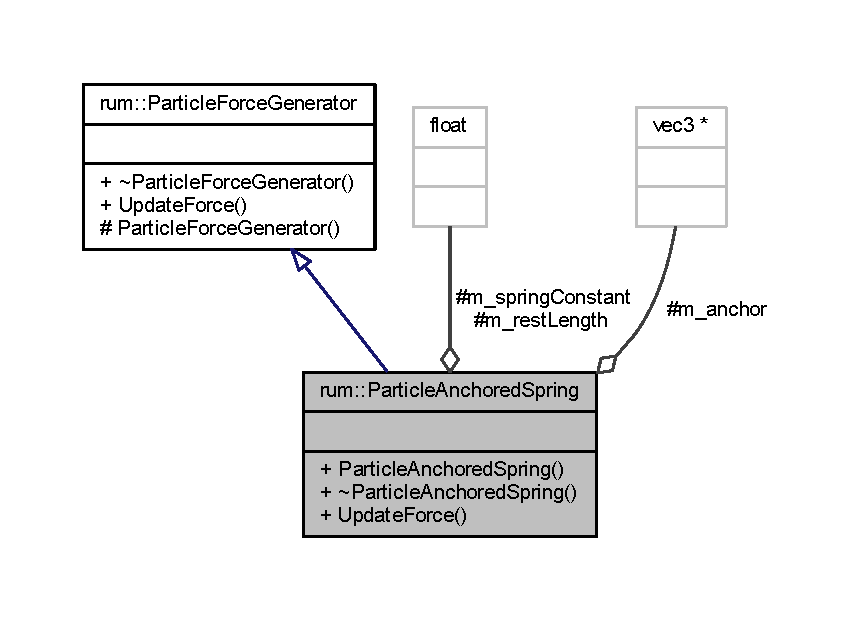
\includegraphics[width=350pt]{classrum_1_1_particle_anchored_spring__coll__graph}
\end{center}
\end{figure}
\subsection*{Public Member Functions}
\begin{DoxyCompactItemize}
\item 
\hyperlink{classrum_1_1_particle_anchored_spring_af0057780e9cc36a2c3e80d5d2ced533b}{Particle\+Anchored\+Spring} (glm\+::vec3 $\ast$anchor, \hyperlink{namespacerum_a7e8cca23573d5eaead0f138cbaa4862c}{real} spring\+Constant, \hyperlink{namespacerum_a7e8cca23573d5eaead0f138cbaa4862c}{real} rest\+Length)
\item 
\hyperlink{classrum_1_1_particle_anchored_spring_a590f7f2dbb306ba4ac5cb7963c8dbf22}{$\sim$\+Particle\+Anchored\+Spring} ()
\item 
virtual void \hyperlink{classrum_1_1_particle_anchored_spring_aa4fcab6f3de51c6b89f3a65b80814cc6}{Update\+Force} (\hyperlink{classrum_1_1_particle}{Particle} $\ast$particle, \hyperlink{namespacerum_a7e8cca23573d5eaead0f138cbaa4862c}{real} duration)
\end{DoxyCompactItemize}
\subsection*{Protected Attributes}
\begin{DoxyCompactItemize}
\item 
glm\+::vec3 $\ast$ \hyperlink{classrum_1_1_particle_anchored_spring_a33813234e4924860ce0f5ee29efd5c96}{m\+\_\+anchor}
\item 
\hyperlink{namespacerum_a7e8cca23573d5eaead0f138cbaa4862c}{real} \hyperlink{classrum_1_1_particle_anchored_spring_a1f5b5cc0af0815b1d7d9902c515f9ed8}{m\+\_\+spring\+Constant}
\item 
\hyperlink{namespacerum_a7e8cca23573d5eaead0f138cbaa4862c}{real} \hyperlink{classrum_1_1_particle_anchored_spring_ae0b4ab273dfd453b9e871ec1371d8ab8}{m\+\_\+rest\+Length}
\end{DoxyCompactItemize}
\subsection*{Additional Inherited Members}


\subsection{Constructor \& Destructor Documentation}
\mbox{\Hypertarget{classrum_1_1_particle_anchored_spring_af0057780e9cc36a2c3e80d5d2ced533b}\label{classrum_1_1_particle_anchored_spring_af0057780e9cc36a2c3e80d5d2ced533b}} 
\index{rum\+::\+Particle\+Anchored\+Spring@{rum\+::\+Particle\+Anchored\+Spring}!Particle\+Anchored\+Spring@{Particle\+Anchored\+Spring}}
\index{Particle\+Anchored\+Spring@{Particle\+Anchored\+Spring}!rum\+::\+Particle\+Anchored\+Spring@{rum\+::\+Particle\+Anchored\+Spring}}
\subsubsection{\texorpdfstring{Particle\+Anchored\+Spring()}{ParticleAnchoredSpring()}}
{\footnotesize\ttfamily rum\+::\+Particle\+Anchored\+Spring\+::\+Particle\+Anchored\+Spring (\begin{DoxyParamCaption}\item[{glm\+::vec3 $\ast$}]{anchor,  }\item[{\hyperlink{namespacerum_a7e8cca23573d5eaead0f138cbaa4862c}{real}}]{spring\+Constant,  }\item[{\hyperlink{namespacerum_a7e8cca23573d5eaead0f138cbaa4862c}{real}}]{rest\+Length }\end{DoxyParamCaption})\hspace{0.3cm}{\ttfamily [explicit]}}

\mbox{\Hypertarget{classrum_1_1_particle_anchored_spring_a590f7f2dbb306ba4ac5cb7963c8dbf22}\label{classrum_1_1_particle_anchored_spring_a590f7f2dbb306ba4ac5cb7963c8dbf22}} 
\index{rum\+::\+Particle\+Anchored\+Spring@{rum\+::\+Particle\+Anchored\+Spring}!````~Particle\+Anchored\+Spring@{$\sim$\+Particle\+Anchored\+Spring}}
\index{````~Particle\+Anchored\+Spring@{$\sim$\+Particle\+Anchored\+Spring}!rum\+::\+Particle\+Anchored\+Spring@{rum\+::\+Particle\+Anchored\+Spring}}
\subsubsection{\texorpdfstring{$\sim$\+Particle\+Anchored\+Spring()}{~ParticleAnchoredSpring()}}
{\footnotesize\ttfamily rum\+::\+Particle\+Anchored\+Spring\+::$\sim$\+Particle\+Anchored\+Spring (\begin{DoxyParamCaption}{ }\end{DoxyParamCaption})}



\subsection{Member Function Documentation}
\mbox{\Hypertarget{classrum_1_1_particle_anchored_spring_aa4fcab6f3de51c6b89f3a65b80814cc6}\label{classrum_1_1_particle_anchored_spring_aa4fcab6f3de51c6b89f3a65b80814cc6}} 
\index{rum\+::\+Particle\+Anchored\+Spring@{rum\+::\+Particle\+Anchored\+Spring}!Update\+Force@{Update\+Force}}
\index{Update\+Force@{Update\+Force}!rum\+::\+Particle\+Anchored\+Spring@{rum\+::\+Particle\+Anchored\+Spring}}
\subsubsection{\texorpdfstring{Update\+Force()}{UpdateForce()}}
{\footnotesize\ttfamily void rum\+::\+Particle\+Anchored\+Spring\+::\+Update\+Force (\begin{DoxyParamCaption}\item[{\hyperlink{classrum_1_1_particle}{Particle} $\ast$}]{particle,  }\item[{\hyperlink{namespacerum_a7e8cca23573d5eaead0f138cbaa4862c}{real}}]{duration }\end{DoxyParamCaption})\hspace{0.3cm}{\ttfamily [virtual]}}



Implements \hyperlink{classrum_1_1_particle_force_generator_aca758295718deb8569796185ccbe8d54}{rum\+::\+Particle\+Force\+Generator}.



\subsection{Member Data Documentation}
\mbox{\Hypertarget{classrum_1_1_particle_anchored_spring_a33813234e4924860ce0f5ee29efd5c96}\label{classrum_1_1_particle_anchored_spring_a33813234e4924860ce0f5ee29efd5c96}} 
\index{rum\+::\+Particle\+Anchored\+Spring@{rum\+::\+Particle\+Anchored\+Spring}!m\+\_\+anchor@{m\+\_\+anchor}}
\index{m\+\_\+anchor@{m\+\_\+anchor}!rum\+::\+Particle\+Anchored\+Spring@{rum\+::\+Particle\+Anchored\+Spring}}
\subsubsection{\texorpdfstring{m\+\_\+anchor}{m\_anchor}}
{\footnotesize\ttfamily glm\+::vec3$\ast$ rum\+::\+Particle\+Anchored\+Spring\+::m\+\_\+anchor\hspace{0.3cm}{\ttfamily [protected]}}

\mbox{\Hypertarget{classrum_1_1_particle_anchored_spring_ae0b4ab273dfd453b9e871ec1371d8ab8}\label{classrum_1_1_particle_anchored_spring_ae0b4ab273dfd453b9e871ec1371d8ab8}} 
\index{rum\+::\+Particle\+Anchored\+Spring@{rum\+::\+Particle\+Anchored\+Spring}!m\+\_\+rest\+Length@{m\+\_\+rest\+Length}}
\index{m\+\_\+rest\+Length@{m\+\_\+rest\+Length}!rum\+::\+Particle\+Anchored\+Spring@{rum\+::\+Particle\+Anchored\+Spring}}
\subsubsection{\texorpdfstring{m\+\_\+rest\+Length}{m\_restLength}}
{\footnotesize\ttfamily \hyperlink{namespacerum_a7e8cca23573d5eaead0f138cbaa4862c}{real} rum\+::\+Particle\+Anchored\+Spring\+::m\+\_\+rest\+Length\hspace{0.3cm}{\ttfamily [protected]}}

\mbox{\Hypertarget{classrum_1_1_particle_anchored_spring_a1f5b5cc0af0815b1d7d9902c515f9ed8}\label{classrum_1_1_particle_anchored_spring_a1f5b5cc0af0815b1d7d9902c515f9ed8}} 
\index{rum\+::\+Particle\+Anchored\+Spring@{rum\+::\+Particle\+Anchored\+Spring}!m\+\_\+spring\+Constant@{m\+\_\+spring\+Constant}}
\index{m\+\_\+spring\+Constant@{m\+\_\+spring\+Constant}!rum\+::\+Particle\+Anchored\+Spring@{rum\+::\+Particle\+Anchored\+Spring}}
\subsubsection{\texorpdfstring{m\+\_\+spring\+Constant}{m\_springConstant}}
{\footnotesize\ttfamily \hyperlink{namespacerum_a7e8cca23573d5eaead0f138cbaa4862c}{real} rum\+::\+Particle\+Anchored\+Spring\+::m\+\_\+spring\+Constant\hspace{0.3cm}{\ttfamily [protected]}}



The documentation for this class was generated from the following files\+:\begin{DoxyCompactItemize}
\item 
F\+:/\+Library/\+Documents/\+Job/\+Forschungsmaster/\+Rumble3\+D/\+Rumble3\+D/include/\+R3\+D/\+Particle\+Engine/\hyperlink{_particle_anchored_spring_8h}{Particle\+Anchored\+Spring.\+h}\item 
F\+:/\+Library/\+Documents/\+Job/\+Forschungsmaster/\+Rumble3\+D/\+Rumble3\+D/src/\+Particle\+Engine/\hyperlink{_particle_anchored_spring_8cpp}{Particle\+Anchored\+Spring.\+cpp}\end{DoxyCompactItemize}

\hypertarget{classrum_1_1_particle_bungee}{}\section{rum\+:\+:Particle\+Bungee Class Reference}
\label{classrum_1_1_particle_bungee}\index{rum\+::\+Particle\+Bungee@{rum\+::\+Particle\+Bungee}}


{\ttfamily \#include $<$Particle\+Bungee.\+h$>$}



Inheritance diagram for rum\+:\+:Particle\+Bungee\+:\nopagebreak
\begin{figure}[H]
\begin{center}
\leavevmode
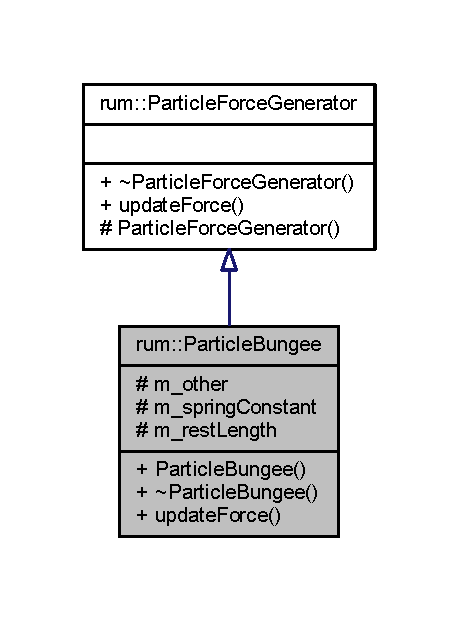
\includegraphics[width=220pt]{classrum_1_1_particle_bungee__inherit__graph}
\end{center}
\end{figure}


Collaboration diagram for rum\+:\+:Particle\+Bungee\+:\nopagebreak
\begin{figure}[H]
\begin{center}
\leavevmode
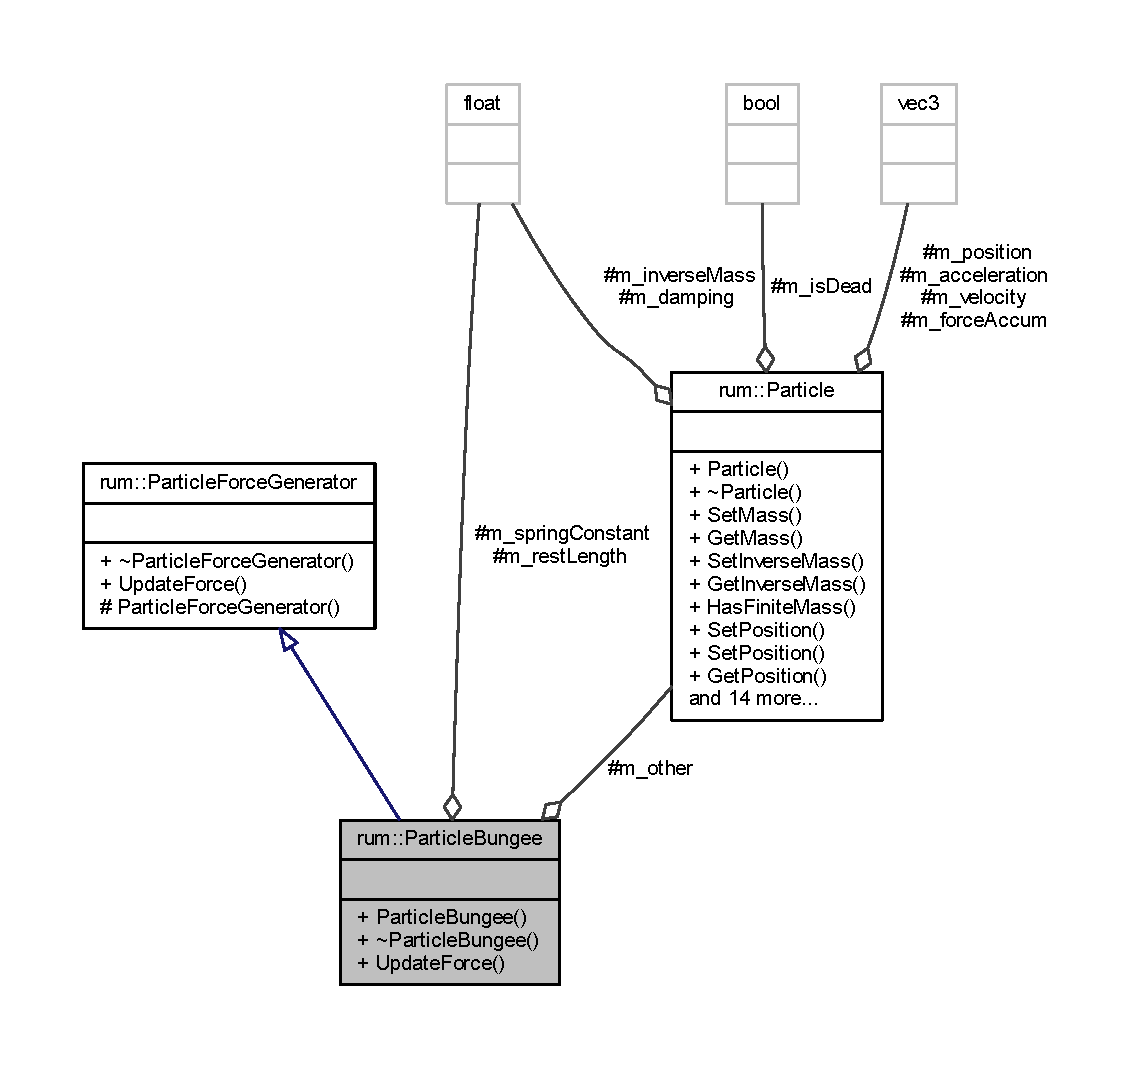
\includegraphics[width=350pt]{classrum_1_1_particle_bungee__coll__graph}
\end{center}
\end{figure}
\subsection*{Public Member Functions}
\begin{DoxyCompactItemize}
\item 
\hyperlink{classrum_1_1_particle_bungee_a8908b5c848fb6ebc45f420e0924e033e}{Particle\+Bungee} (\hyperlink{classrum_1_1_particle}{Particle} $\ast$other, \hyperlink{namespacerum_a7e8cca23573d5eaead0f138cbaa4862c}{real} spring\+Constant, \hyperlink{namespacerum_a7e8cca23573d5eaead0f138cbaa4862c}{real} rest\+Length)
\item 
\hyperlink{classrum_1_1_particle_bungee_aaff4a95227aaec80896d0030ded6c6b3}{$\sim$\+Particle\+Bungee} ()
\item 
virtual void \hyperlink{classrum_1_1_particle_bungee_a631e7f4c92c881b9a62471e2f75e2a2c}{Update\+Force} (\hyperlink{classrum_1_1_particle}{Particle} $\ast$particle, \hyperlink{namespacerum_a7e8cca23573d5eaead0f138cbaa4862c}{real} duration)
\end{DoxyCompactItemize}
\subsection*{Protected Attributes}
\begin{DoxyCompactItemize}
\item 
\hyperlink{classrum_1_1_particle}{Particle} $\ast$ \hyperlink{classrum_1_1_particle_bungee_a86d11a089a58dca74854d94630d9f125}{m\+\_\+other}
\item 
\hyperlink{namespacerum_a7e8cca23573d5eaead0f138cbaa4862c}{real} \hyperlink{classrum_1_1_particle_bungee_a4a77b3fb166e4e56dc3a57f5807d985f}{m\+\_\+spring\+Constant}
\item 
\hyperlink{namespacerum_a7e8cca23573d5eaead0f138cbaa4862c}{real} \hyperlink{classrum_1_1_particle_bungee_a4392eb2dc76c9371acfddcb852bb3737}{m\+\_\+rest\+Length}
\end{DoxyCompactItemize}
\subsection*{Additional Inherited Members}


\subsection{Constructor \& Destructor Documentation}
\mbox{\Hypertarget{classrum_1_1_particle_bungee_a8908b5c848fb6ebc45f420e0924e033e}\label{classrum_1_1_particle_bungee_a8908b5c848fb6ebc45f420e0924e033e}} 
\index{rum\+::\+Particle\+Bungee@{rum\+::\+Particle\+Bungee}!Particle\+Bungee@{Particle\+Bungee}}
\index{Particle\+Bungee@{Particle\+Bungee}!rum\+::\+Particle\+Bungee@{rum\+::\+Particle\+Bungee}}
\subsubsection{\texorpdfstring{Particle\+Bungee()}{ParticleBungee()}}
{\footnotesize\ttfamily rum\+::\+Particle\+Bungee\+::\+Particle\+Bungee (\begin{DoxyParamCaption}\item[{\hyperlink{classrum_1_1_particle}{Particle} $\ast$}]{other,  }\item[{\hyperlink{namespacerum_a7e8cca23573d5eaead0f138cbaa4862c}{real}}]{spring\+Constant,  }\item[{\hyperlink{namespacerum_a7e8cca23573d5eaead0f138cbaa4862c}{real}}]{rest\+Length }\end{DoxyParamCaption})\hspace{0.3cm}{\ttfamily [explicit]}}

\mbox{\Hypertarget{classrum_1_1_particle_bungee_aaff4a95227aaec80896d0030ded6c6b3}\label{classrum_1_1_particle_bungee_aaff4a95227aaec80896d0030ded6c6b3}} 
\index{rum\+::\+Particle\+Bungee@{rum\+::\+Particle\+Bungee}!````~Particle\+Bungee@{$\sim$\+Particle\+Bungee}}
\index{````~Particle\+Bungee@{$\sim$\+Particle\+Bungee}!rum\+::\+Particle\+Bungee@{rum\+::\+Particle\+Bungee}}
\subsubsection{\texorpdfstring{$\sim$\+Particle\+Bungee()}{~ParticleBungee()}}
{\footnotesize\ttfamily rum\+::\+Particle\+Bungee\+::$\sim$\+Particle\+Bungee (\begin{DoxyParamCaption}{ }\end{DoxyParamCaption})}



\subsection{Member Function Documentation}
\mbox{\Hypertarget{classrum_1_1_particle_bungee_a631e7f4c92c881b9a62471e2f75e2a2c}\label{classrum_1_1_particle_bungee_a631e7f4c92c881b9a62471e2f75e2a2c}} 
\index{rum\+::\+Particle\+Bungee@{rum\+::\+Particle\+Bungee}!Update\+Force@{Update\+Force}}
\index{Update\+Force@{Update\+Force}!rum\+::\+Particle\+Bungee@{rum\+::\+Particle\+Bungee}}
\subsubsection{\texorpdfstring{Update\+Force()}{UpdateForce()}}
{\footnotesize\ttfamily void rum\+::\+Particle\+Bungee\+::\+Update\+Force (\begin{DoxyParamCaption}\item[{\hyperlink{classrum_1_1_particle}{Particle} $\ast$}]{particle,  }\item[{\hyperlink{namespacerum_a7e8cca23573d5eaead0f138cbaa4862c}{real}}]{duration }\end{DoxyParamCaption})\hspace{0.3cm}{\ttfamily [virtual]}}



Implements \hyperlink{classrum_1_1_particle_force_generator_aca758295718deb8569796185ccbe8d54}{rum\+::\+Particle\+Force\+Generator}.



\subsection{Member Data Documentation}
\mbox{\Hypertarget{classrum_1_1_particle_bungee_a86d11a089a58dca74854d94630d9f125}\label{classrum_1_1_particle_bungee_a86d11a089a58dca74854d94630d9f125}} 
\index{rum\+::\+Particle\+Bungee@{rum\+::\+Particle\+Bungee}!m\+\_\+other@{m\+\_\+other}}
\index{m\+\_\+other@{m\+\_\+other}!rum\+::\+Particle\+Bungee@{rum\+::\+Particle\+Bungee}}
\subsubsection{\texorpdfstring{m\+\_\+other}{m\_other}}
{\footnotesize\ttfamily \hyperlink{classrum_1_1_particle}{Particle}$\ast$ rum\+::\+Particle\+Bungee\+::m\+\_\+other\hspace{0.3cm}{\ttfamily [protected]}}

\mbox{\Hypertarget{classrum_1_1_particle_bungee_a4392eb2dc76c9371acfddcb852bb3737}\label{classrum_1_1_particle_bungee_a4392eb2dc76c9371acfddcb852bb3737}} 
\index{rum\+::\+Particle\+Bungee@{rum\+::\+Particle\+Bungee}!m\+\_\+rest\+Length@{m\+\_\+rest\+Length}}
\index{m\+\_\+rest\+Length@{m\+\_\+rest\+Length}!rum\+::\+Particle\+Bungee@{rum\+::\+Particle\+Bungee}}
\subsubsection{\texorpdfstring{m\+\_\+rest\+Length}{m\_restLength}}
{\footnotesize\ttfamily \hyperlink{namespacerum_a7e8cca23573d5eaead0f138cbaa4862c}{real} rum\+::\+Particle\+Bungee\+::m\+\_\+rest\+Length\hspace{0.3cm}{\ttfamily [protected]}}

\mbox{\Hypertarget{classrum_1_1_particle_bungee_a4a77b3fb166e4e56dc3a57f5807d985f}\label{classrum_1_1_particle_bungee_a4a77b3fb166e4e56dc3a57f5807d985f}} 
\index{rum\+::\+Particle\+Bungee@{rum\+::\+Particle\+Bungee}!m\+\_\+spring\+Constant@{m\+\_\+spring\+Constant}}
\index{m\+\_\+spring\+Constant@{m\+\_\+spring\+Constant}!rum\+::\+Particle\+Bungee@{rum\+::\+Particle\+Bungee}}
\subsubsection{\texorpdfstring{m\+\_\+spring\+Constant}{m\_springConstant}}
{\footnotesize\ttfamily \hyperlink{namespacerum_a7e8cca23573d5eaead0f138cbaa4862c}{real} rum\+::\+Particle\+Bungee\+::m\+\_\+spring\+Constant\hspace{0.3cm}{\ttfamily [protected]}}



The documentation for this class was generated from the following files\+:\begin{DoxyCompactItemize}
\item 
F\+:/\+Library/\+Documents/\+Job/\+Forschungsmaster/\+Rumble3\+D/\+Rumble3\+D/include/\+R3\+D/\+Particle\+Engine/\hyperlink{_particle_bungee_8h}{Particle\+Bungee.\+h}\item 
F\+:/\+Library/\+Documents/\+Job/\+Forschungsmaster/\+Rumble3\+D/\+Rumble3\+D/src/\+Particle\+Engine/\hyperlink{_particle_bungee_8cpp}{Particle\+Bungee.\+cpp}\end{DoxyCompactItemize}

\hypertarget{classrum_1_1_particle_buoyancy}{}\section{rum\+:\+:Particle\+Buoyancy Class Reference}
\label{classrum_1_1_particle_buoyancy}\index{rum\+::\+Particle\+Buoyancy@{rum\+::\+Particle\+Buoyancy}}


{\ttfamily \#include $<$Particle\+Buoyancy.\+h$>$}



Inheritance diagram for rum\+:\+:Particle\+Buoyancy\+:\nopagebreak
\begin{figure}[H]
\begin{center}
\leavevmode
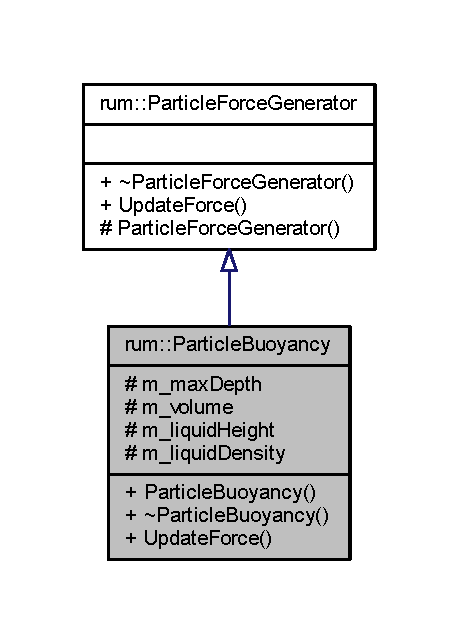
\includegraphics[width=220pt]{classrum_1_1_particle_buoyancy__inherit__graph}
\end{center}
\end{figure}


Collaboration diagram for rum\+:\+:Particle\+Buoyancy\+:\nopagebreak
\begin{figure}[H]
\begin{center}
\leavevmode
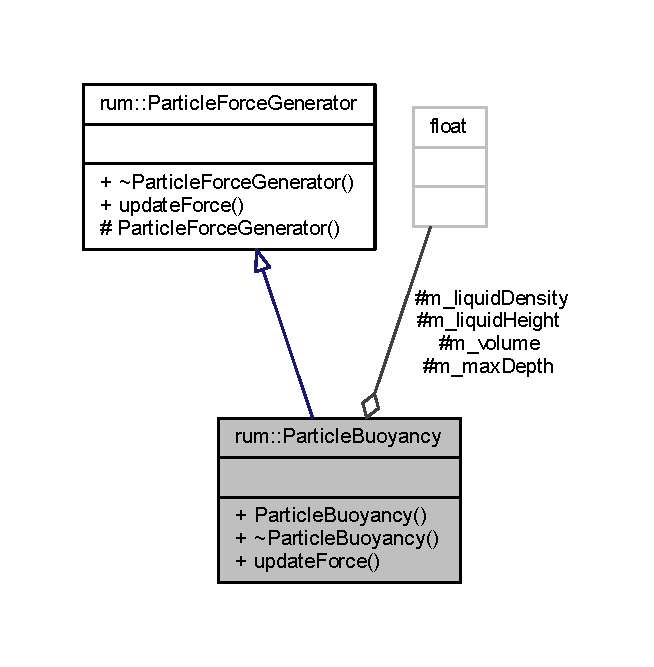
\includegraphics[width=314pt]{classrum_1_1_particle_buoyancy__coll__graph}
\end{center}
\end{figure}
\subsection*{Public Member Functions}
\begin{DoxyCompactItemize}
\item 
\mbox{\hyperlink{classrum_1_1_particle_buoyancy_a25df269bba530e8275ee0e22e9fce166}{Particle\+Buoyancy}} (\mbox{\hyperlink{namespacerum_a7e8cca23573d5eaead0f138cbaa4862c}{real}} max\+Depth, \mbox{\hyperlink{namespacerum_a7e8cca23573d5eaead0f138cbaa4862c}{real}} volume, \mbox{\hyperlink{namespacerum_a7e8cca23573d5eaead0f138cbaa4862c}{real}} liquid\+Height, \mbox{\hyperlink{namespacerum_a7e8cca23573d5eaead0f138cbaa4862c}{real}} liquid\+Density=\mbox{\hyperlink{namespacerum_a7e8cca23573d5eaead0f138cbaa4862c}{real}}(1000.\+0f))
\item 
\mbox{\hyperlink{classrum_1_1_particle_buoyancy_a892e6f064e5eb1be8e7d2af8c76b856c}{$\sim$\+Particle\+Buoyancy}} ()
\item 
void \mbox{\hyperlink{classrum_1_1_particle_buoyancy_a192992c47ce2b47fd06d0224e0cf86f4}{update\+Force}} (\mbox{\hyperlink{classrum_1_1_particle}{Particle}} $\ast$particle, \mbox{\hyperlink{namespacerum_a7e8cca23573d5eaead0f138cbaa4862c}{real}} duration) override
\end{DoxyCompactItemize}
\subsection*{Protected Attributes}
\begin{DoxyCompactItemize}
\item 
\mbox{\hyperlink{namespacerum_a7e8cca23573d5eaead0f138cbaa4862c}{real}} \mbox{\hyperlink{classrum_1_1_particle_buoyancy_af29f25245a785fc1bceafeac08728370}{m\+\_\+max\+Depth}}
\item 
\mbox{\hyperlink{namespacerum_a7e8cca23573d5eaead0f138cbaa4862c}{real}} \mbox{\hyperlink{classrum_1_1_particle_buoyancy_acb0a75c58de8ddede0b4be9939917c32}{m\+\_\+volume}}
\item 
\mbox{\hyperlink{namespacerum_a7e8cca23573d5eaead0f138cbaa4862c}{real}} \mbox{\hyperlink{classrum_1_1_particle_buoyancy_a220309bad493fc0d090bd3e91d9f4acb}{m\+\_\+liquid\+Height}}
\item 
\mbox{\hyperlink{namespacerum_a7e8cca23573d5eaead0f138cbaa4862c}{real}} \mbox{\hyperlink{classrum_1_1_particle_buoyancy_a8e347c9390d2eb5e4340f6e3c9d8d332}{m\+\_\+liquid\+Density}}
\end{DoxyCompactItemize}
\subsection*{Additional Inherited Members}


\subsection{Constructor \& Destructor Documentation}
\mbox{\Hypertarget{classrum_1_1_particle_buoyancy_a25df269bba530e8275ee0e22e9fce166}\label{classrum_1_1_particle_buoyancy_a25df269bba530e8275ee0e22e9fce166}} 
\index{rum\+::\+Particle\+Buoyancy@{rum\+::\+Particle\+Buoyancy}!Particle\+Buoyancy@{Particle\+Buoyancy}}
\index{Particle\+Buoyancy@{Particle\+Buoyancy}!rum\+::\+Particle\+Buoyancy@{rum\+::\+Particle\+Buoyancy}}
\subsubsection{\texorpdfstring{Particle\+Buoyancy()}{ParticleBuoyancy()}}
{\footnotesize\ttfamily rum\+::\+Particle\+Buoyancy\+::\+Particle\+Buoyancy (\begin{DoxyParamCaption}\item[{\mbox{\hyperlink{namespacerum_a7e8cca23573d5eaead0f138cbaa4862c}{real}}}]{max\+Depth,  }\item[{\mbox{\hyperlink{namespacerum_a7e8cca23573d5eaead0f138cbaa4862c}{real}}}]{volume,  }\item[{\mbox{\hyperlink{namespacerum_a7e8cca23573d5eaead0f138cbaa4862c}{real}}}]{liquid\+Height,  }\item[{\mbox{\hyperlink{namespacerum_a7e8cca23573d5eaead0f138cbaa4862c}{real}}}]{liquid\+Density = {\ttfamily \mbox{\hyperlink{namespacerum_a7e8cca23573d5eaead0f138cbaa4862c}{real}}(1000.0f)} }\end{DoxyParamCaption})\hspace{0.3cm}{\ttfamily [explicit]}}

\mbox{\Hypertarget{classrum_1_1_particle_buoyancy_a892e6f064e5eb1be8e7d2af8c76b856c}\label{classrum_1_1_particle_buoyancy_a892e6f064e5eb1be8e7d2af8c76b856c}} 
\index{rum\+::\+Particle\+Buoyancy@{rum\+::\+Particle\+Buoyancy}!````~Particle\+Buoyancy@{$\sim$\+Particle\+Buoyancy}}
\index{````~Particle\+Buoyancy@{$\sim$\+Particle\+Buoyancy}!rum\+::\+Particle\+Buoyancy@{rum\+::\+Particle\+Buoyancy}}
\subsubsection{\texorpdfstring{$\sim$\+Particle\+Buoyancy()}{~ParticleBuoyancy()}}
{\footnotesize\ttfamily rum\+::\+Particle\+Buoyancy\+::$\sim$\+Particle\+Buoyancy (\begin{DoxyParamCaption}{ }\end{DoxyParamCaption})}



\subsection{Member Function Documentation}
\mbox{\Hypertarget{classrum_1_1_particle_buoyancy_a192992c47ce2b47fd06d0224e0cf86f4}\label{classrum_1_1_particle_buoyancy_a192992c47ce2b47fd06d0224e0cf86f4}} 
\index{rum\+::\+Particle\+Buoyancy@{rum\+::\+Particle\+Buoyancy}!update\+Force@{update\+Force}}
\index{update\+Force@{update\+Force}!rum\+::\+Particle\+Buoyancy@{rum\+::\+Particle\+Buoyancy}}
\subsubsection{\texorpdfstring{update\+Force()}{updateForce()}}
{\footnotesize\ttfamily void rum\+::\+Particle\+Buoyancy\+::update\+Force (\begin{DoxyParamCaption}\item[{\mbox{\hyperlink{classrum_1_1_particle}{Particle}} $\ast$}]{particle,  }\item[{\mbox{\hyperlink{namespacerum_a7e8cca23573d5eaead0f138cbaa4862c}{real}}}]{duration }\end{DoxyParamCaption})\hspace{0.3cm}{\ttfamily [override]}, {\ttfamily [virtual]}}



Implements \mbox{\hyperlink{classrum_1_1_particle_force_generator_af7abcafb9527220988ec4b9dde817b34}{rum\+::\+Particle\+Force\+Generator}}.



\subsection{Member Data Documentation}
\mbox{\Hypertarget{classrum_1_1_particle_buoyancy_a8e347c9390d2eb5e4340f6e3c9d8d332}\label{classrum_1_1_particle_buoyancy_a8e347c9390d2eb5e4340f6e3c9d8d332}} 
\index{rum\+::\+Particle\+Buoyancy@{rum\+::\+Particle\+Buoyancy}!m\+\_\+liquid\+Density@{m\+\_\+liquid\+Density}}
\index{m\+\_\+liquid\+Density@{m\+\_\+liquid\+Density}!rum\+::\+Particle\+Buoyancy@{rum\+::\+Particle\+Buoyancy}}
\subsubsection{\texorpdfstring{m\+\_\+liquid\+Density}{m\_liquidDensity}}
{\footnotesize\ttfamily \mbox{\hyperlink{namespacerum_a7e8cca23573d5eaead0f138cbaa4862c}{real}} rum\+::\+Particle\+Buoyancy\+::m\+\_\+liquid\+Density\hspace{0.3cm}{\ttfamily [protected]}}

\mbox{\Hypertarget{classrum_1_1_particle_buoyancy_a220309bad493fc0d090bd3e91d9f4acb}\label{classrum_1_1_particle_buoyancy_a220309bad493fc0d090bd3e91d9f4acb}} 
\index{rum\+::\+Particle\+Buoyancy@{rum\+::\+Particle\+Buoyancy}!m\+\_\+liquid\+Height@{m\+\_\+liquid\+Height}}
\index{m\+\_\+liquid\+Height@{m\+\_\+liquid\+Height}!rum\+::\+Particle\+Buoyancy@{rum\+::\+Particle\+Buoyancy}}
\subsubsection{\texorpdfstring{m\+\_\+liquid\+Height}{m\_liquidHeight}}
{\footnotesize\ttfamily \mbox{\hyperlink{namespacerum_a7e8cca23573d5eaead0f138cbaa4862c}{real}} rum\+::\+Particle\+Buoyancy\+::m\+\_\+liquid\+Height\hspace{0.3cm}{\ttfamily [protected]}}

\mbox{\Hypertarget{classrum_1_1_particle_buoyancy_af29f25245a785fc1bceafeac08728370}\label{classrum_1_1_particle_buoyancy_af29f25245a785fc1bceafeac08728370}} 
\index{rum\+::\+Particle\+Buoyancy@{rum\+::\+Particle\+Buoyancy}!m\+\_\+max\+Depth@{m\+\_\+max\+Depth}}
\index{m\+\_\+max\+Depth@{m\+\_\+max\+Depth}!rum\+::\+Particle\+Buoyancy@{rum\+::\+Particle\+Buoyancy}}
\subsubsection{\texorpdfstring{m\+\_\+max\+Depth}{m\_maxDepth}}
{\footnotesize\ttfamily \mbox{\hyperlink{namespacerum_a7e8cca23573d5eaead0f138cbaa4862c}{real}} rum\+::\+Particle\+Buoyancy\+::m\+\_\+max\+Depth\hspace{0.3cm}{\ttfamily [protected]}}

\mbox{\Hypertarget{classrum_1_1_particle_buoyancy_acb0a75c58de8ddede0b4be9939917c32}\label{classrum_1_1_particle_buoyancy_acb0a75c58de8ddede0b4be9939917c32}} 
\index{rum\+::\+Particle\+Buoyancy@{rum\+::\+Particle\+Buoyancy}!m\+\_\+volume@{m\+\_\+volume}}
\index{m\+\_\+volume@{m\+\_\+volume}!rum\+::\+Particle\+Buoyancy@{rum\+::\+Particle\+Buoyancy}}
\subsubsection{\texorpdfstring{m\+\_\+volume}{m\_volume}}
{\footnotesize\ttfamily \mbox{\hyperlink{namespacerum_a7e8cca23573d5eaead0f138cbaa4862c}{real}} rum\+::\+Particle\+Buoyancy\+::m\+\_\+volume\hspace{0.3cm}{\ttfamily [protected]}}



The documentation for this class was generated from the following files\+:\begin{DoxyCompactItemize}
\item 
D\+:/\+Library/\+Documents/\+Job/\+Forschungsmaster/\+Projekte/\+Rumble3\+D/\+Rumble3\+D/include/\+R3\+D/\+Particle\+Engine/\mbox{\hyperlink{_particle_buoyancy_8h}{Particle\+Buoyancy.\+h}}\item 
D\+:/\+Library/\+Documents/\+Job/\+Forschungsmaster/\+Projekte/\+Rumble3\+D/\+Rumble3\+D/src/\+Particle\+Engine/\mbox{\hyperlink{_particle_buoyancy_8cpp}{Particle\+Buoyancy.\+cpp}}\end{DoxyCompactItemize}

\hypertarget{classrum_1_1_particle_cable}{}\section{rum\+:\+:Particle\+Cable Class Reference}
\label{classrum_1_1_particle_cable}\index{rum\+::\+Particle\+Cable@{rum\+::\+Particle\+Cable}}


{\ttfamily \#include $<$Particle\+Cable.\+h$>$}



Inheritance diagram for rum\+:\+:Particle\+Cable\+:\nopagebreak
\begin{figure}[H]
\begin{center}
\leavevmode
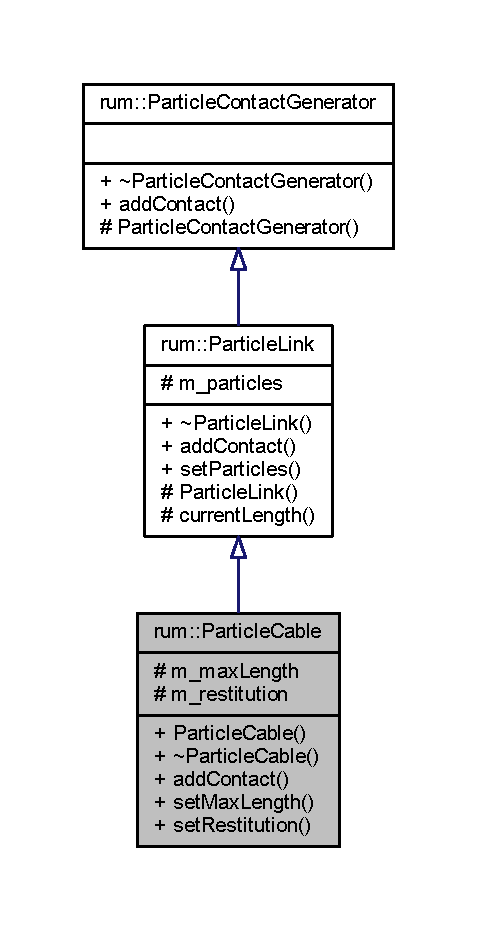
\includegraphics[width=229pt]{classrum_1_1_particle_cable__inherit__graph}
\end{center}
\end{figure}


Collaboration diagram for rum\+:\+:Particle\+Cable\+:\nopagebreak
\begin{figure}[H]
\begin{center}
\leavevmode
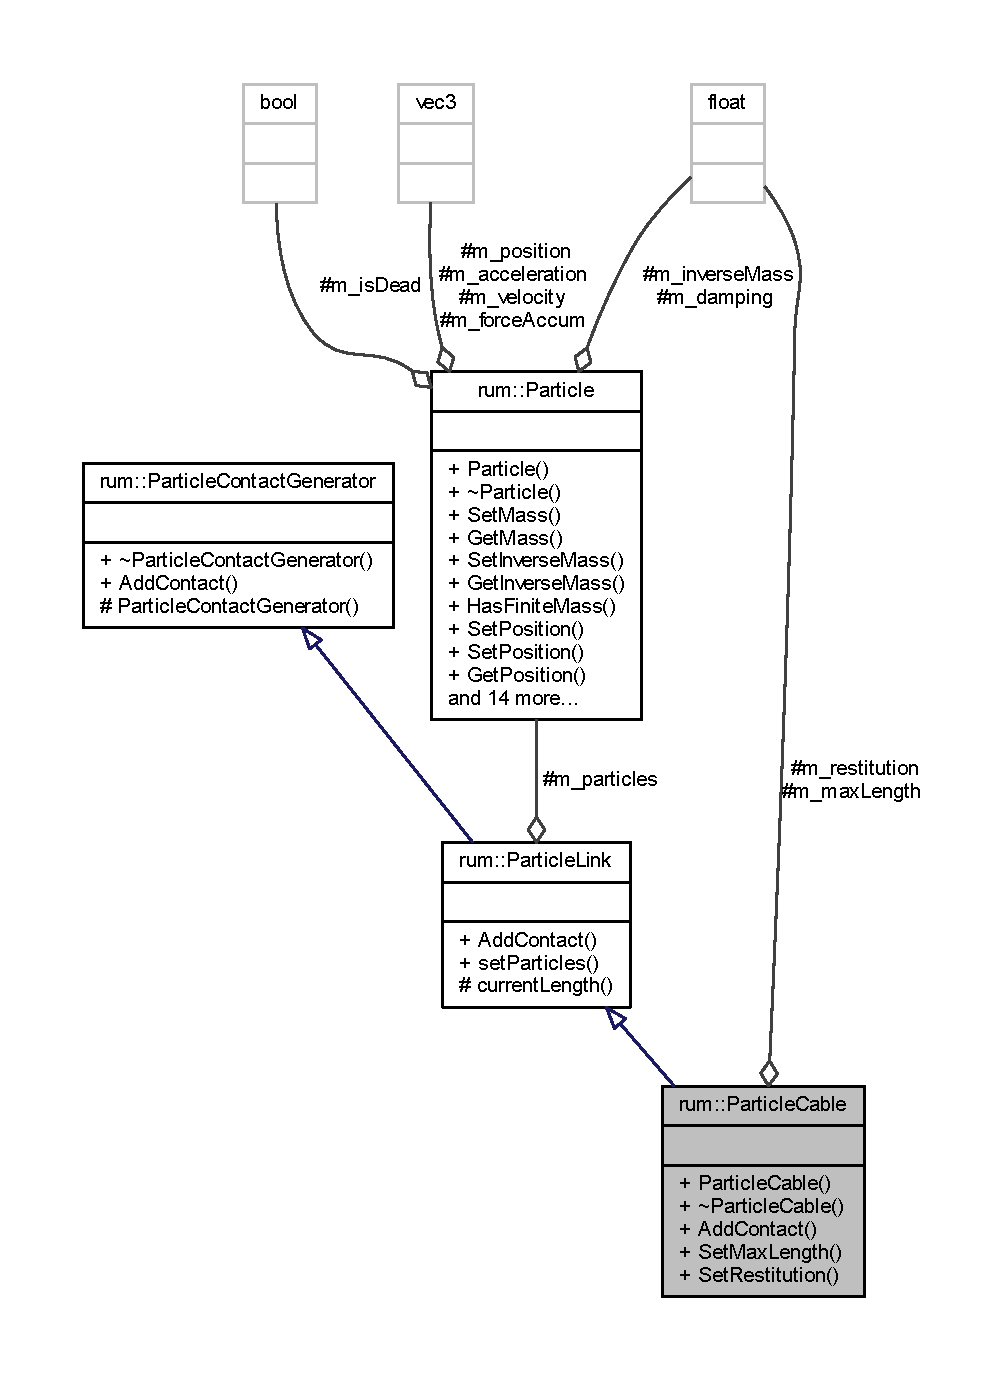
\includegraphics[width=350pt]{classrum_1_1_particle_cable__coll__graph}
\end{center}
\end{figure}
\subsection*{Public Member Functions}
\begin{DoxyCompactItemize}
\item 
\mbox{\hyperlink{classrum_1_1_particle_cable_ad2b529c1d51b6af9f3c2e7f535e64c0c}{Particle\+Cable}} ()
\item 
\mbox{\hyperlink{classrum_1_1_particle_cable_aac2552bf3ddefc5c59fd7953a719b43a}{$\sim$\+Particle\+Cable}} ()
\item 
unsigned int \mbox{\hyperlink{classrum_1_1_particle_cable_a078344be0db7ccc00d326ac767736431}{add\+Contact}} (\mbox{\hyperlink{classrum_1_1_particle_contact}{Particle\+Contact}} $\ast$contact, unsigned int limit) const override
\item 
void \mbox{\hyperlink{classrum_1_1_particle_cable_a3a40cd1d2581bec38d66275af22c9347}{set\+Max\+Length}} (\mbox{\hyperlink{namespacerum_a7e8cca23573d5eaead0f138cbaa4862c}{real}} max\+Length)
\item 
void \mbox{\hyperlink{classrum_1_1_particle_cable_ab6b2076bdb4bd5ab15a695a17649ae56}{set\+Restitution}} (\mbox{\hyperlink{namespacerum_a7e8cca23573d5eaead0f138cbaa4862c}{real}} restitution)
\end{DoxyCompactItemize}
\subsection*{Protected Attributes}
\begin{DoxyCompactItemize}
\item 
\mbox{\hyperlink{namespacerum_a7e8cca23573d5eaead0f138cbaa4862c}{real}} \mbox{\hyperlink{classrum_1_1_particle_cable_a7232daf25d24eff2f98e03918bfbfb7c}{m\+\_\+max\+Length}}
\item 
\mbox{\hyperlink{namespacerum_a7e8cca23573d5eaead0f138cbaa4862c}{real}} \mbox{\hyperlink{classrum_1_1_particle_cable_affbb776b02c85a36d0d0bb1ca6f4234a}{m\+\_\+restitution}}
\end{DoxyCompactItemize}
\subsection*{Additional Inherited Members}


\subsection{Constructor \& Destructor Documentation}
\mbox{\Hypertarget{classrum_1_1_particle_cable_ad2b529c1d51b6af9f3c2e7f535e64c0c}\label{classrum_1_1_particle_cable_ad2b529c1d51b6af9f3c2e7f535e64c0c}} 
\index{rum\+::\+Particle\+Cable@{rum\+::\+Particle\+Cable}!Particle\+Cable@{Particle\+Cable}}
\index{Particle\+Cable@{Particle\+Cable}!rum\+::\+Particle\+Cable@{rum\+::\+Particle\+Cable}}
\subsubsection{\texorpdfstring{Particle\+Cable()}{ParticleCable()}}
{\footnotesize\ttfamily rum\+::\+Particle\+Cable\+::\+Particle\+Cable (\begin{DoxyParamCaption}{ }\end{DoxyParamCaption})\hspace{0.3cm}{\ttfamily [explicit]}}

\mbox{\Hypertarget{classrum_1_1_particle_cable_aac2552bf3ddefc5c59fd7953a719b43a}\label{classrum_1_1_particle_cable_aac2552bf3ddefc5c59fd7953a719b43a}} 
\index{rum\+::\+Particle\+Cable@{rum\+::\+Particle\+Cable}!````~Particle\+Cable@{$\sim$\+Particle\+Cable}}
\index{````~Particle\+Cable@{$\sim$\+Particle\+Cable}!rum\+::\+Particle\+Cable@{rum\+::\+Particle\+Cable}}
\subsubsection{\texorpdfstring{$\sim$\+Particle\+Cable()}{~ParticleCable()}}
{\footnotesize\ttfamily rum\+::\+Particle\+Cable\+::$\sim$\+Particle\+Cable (\begin{DoxyParamCaption}{ }\end{DoxyParamCaption})}



\subsection{Member Function Documentation}
\mbox{\Hypertarget{classrum_1_1_particle_cable_a078344be0db7ccc00d326ac767736431}\label{classrum_1_1_particle_cable_a078344be0db7ccc00d326ac767736431}} 
\index{rum\+::\+Particle\+Cable@{rum\+::\+Particle\+Cable}!add\+Contact@{add\+Contact}}
\index{add\+Contact@{add\+Contact}!rum\+::\+Particle\+Cable@{rum\+::\+Particle\+Cable}}
\subsubsection{\texorpdfstring{add\+Contact()}{addContact()}}
{\footnotesize\ttfamily unsigned int rum\+::\+Particle\+Cable\+::add\+Contact (\begin{DoxyParamCaption}\item[{\mbox{\hyperlink{classrum_1_1_particle_contact}{Particle\+Contact}} $\ast$}]{contact,  }\item[{unsigned int}]{limit }\end{DoxyParamCaption}) const\hspace{0.3cm}{\ttfamily [override]}, {\ttfamily [virtual]}}



Implements \mbox{\hyperlink{classrum_1_1_particle_link_a0da76619bd1d2ae04d5f8173c2883ff2}{rum\+::\+Particle\+Link}}.

\mbox{\Hypertarget{classrum_1_1_particle_cable_a3a40cd1d2581bec38d66275af22c9347}\label{classrum_1_1_particle_cable_a3a40cd1d2581bec38d66275af22c9347}} 
\index{rum\+::\+Particle\+Cable@{rum\+::\+Particle\+Cable}!set\+Max\+Length@{set\+Max\+Length}}
\index{set\+Max\+Length@{set\+Max\+Length}!rum\+::\+Particle\+Cable@{rum\+::\+Particle\+Cable}}
\subsubsection{\texorpdfstring{set\+Max\+Length()}{setMaxLength()}}
{\footnotesize\ttfamily void rum\+::\+Particle\+Cable\+::set\+Max\+Length (\begin{DoxyParamCaption}\item[{\mbox{\hyperlink{namespacerum_a7e8cca23573d5eaead0f138cbaa4862c}{real}}}]{max\+Length }\end{DoxyParamCaption})}

\mbox{\Hypertarget{classrum_1_1_particle_cable_ab6b2076bdb4bd5ab15a695a17649ae56}\label{classrum_1_1_particle_cable_ab6b2076bdb4bd5ab15a695a17649ae56}} 
\index{rum\+::\+Particle\+Cable@{rum\+::\+Particle\+Cable}!set\+Restitution@{set\+Restitution}}
\index{set\+Restitution@{set\+Restitution}!rum\+::\+Particle\+Cable@{rum\+::\+Particle\+Cable}}
\subsubsection{\texorpdfstring{set\+Restitution()}{setRestitution()}}
{\footnotesize\ttfamily void rum\+::\+Particle\+Cable\+::set\+Restitution (\begin{DoxyParamCaption}\item[{\mbox{\hyperlink{namespacerum_a7e8cca23573d5eaead0f138cbaa4862c}{real}}}]{restitution }\end{DoxyParamCaption})}



\subsection{Member Data Documentation}
\mbox{\Hypertarget{classrum_1_1_particle_cable_a7232daf25d24eff2f98e03918bfbfb7c}\label{classrum_1_1_particle_cable_a7232daf25d24eff2f98e03918bfbfb7c}} 
\index{rum\+::\+Particle\+Cable@{rum\+::\+Particle\+Cable}!m\+\_\+max\+Length@{m\+\_\+max\+Length}}
\index{m\+\_\+max\+Length@{m\+\_\+max\+Length}!rum\+::\+Particle\+Cable@{rum\+::\+Particle\+Cable}}
\subsubsection{\texorpdfstring{m\+\_\+max\+Length}{m\_maxLength}}
{\footnotesize\ttfamily \mbox{\hyperlink{namespacerum_a7e8cca23573d5eaead0f138cbaa4862c}{real}} rum\+::\+Particle\+Cable\+::m\+\_\+max\+Length\hspace{0.3cm}{\ttfamily [protected]}}

\mbox{\Hypertarget{classrum_1_1_particle_cable_affbb776b02c85a36d0d0bb1ca6f4234a}\label{classrum_1_1_particle_cable_affbb776b02c85a36d0d0bb1ca6f4234a}} 
\index{rum\+::\+Particle\+Cable@{rum\+::\+Particle\+Cable}!m\+\_\+restitution@{m\+\_\+restitution}}
\index{m\+\_\+restitution@{m\+\_\+restitution}!rum\+::\+Particle\+Cable@{rum\+::\+Particle\+Cable}}
\subsubsection{\texorpdfstring{m\+\_\+restitution}{m\_restitution}}
{\footnotesize\ttfamily \mbox{\hyperlink{namespacerum_a7e8cca23573d5eaead0f138cbaa4862c}{real}} rum\+::\+Particle\+Cable\+::m\+\_\+restitution\hspace{0.3cm}{\ttfamily [protected]}}



The documentation for this class was generated from the following files\+:\begin{DoxyCompactItemize}
\item 
D\+:/\+Library/\+Documents/\+Job/\+Forschungsmaster/\+Projekte/\+Rumble3\+D/\+Rumble3\+D/include/\+R3\+D/\+Particle\+Engine/\mbox{\hyperlink{_particle_cable_8h}{Particle\+Cable.\+h}}\item 
D\+:/\+Library/\+Documents/\+Job/\+Forschungsmaster/\+Projekte/\+Rumble3\+D/\+Rumble3\+D/src/\+Particle\+Engine/\mbox{\hyperlink{_particle_cable_8cpp}{Particle\+Cable.\+cpp}}\end{DoxyCompactItemize}

\hypertarget{classrum_1_1_particle_collision}{}\section{rum\+:\+:Particle\+Collision Class Reference}
\label{classrum_1_1_particle_collision}\index{rum\+::\+Particle\+Collision@{rum\+::\+Particle\+Collision}}


{\ttfamily \#include $<$Particle\+Collision.\+h$>$}



Inheritance diagram for rum\+:\+:Particle\+Collision\+:\nopagebreak
\begin{figure}[H]
\begin{center}
\leavevmode
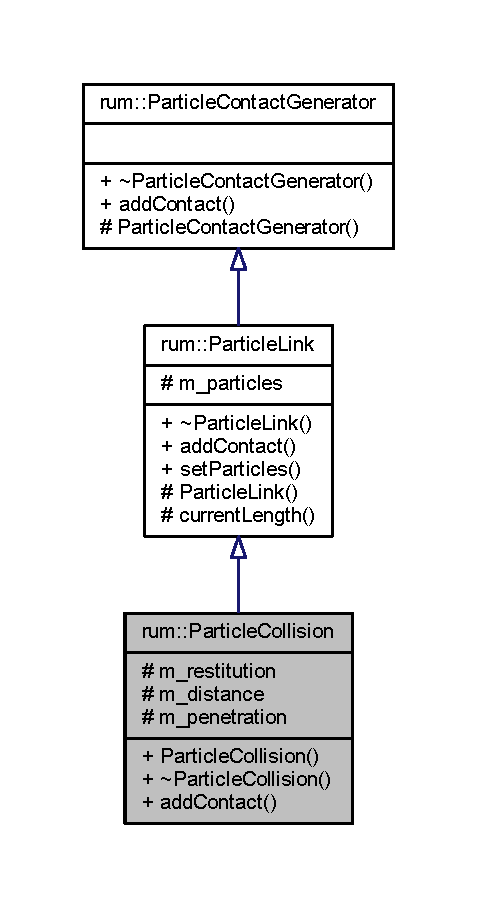
\includegraphics[width=229pt]{classrum_1_1_particle_collision__inherit__graph}
\end{center}
\end{figure}


Collaboration diagram for rum\+:\+:Particle\+Collision\+:\nopagebreak
\begin{figure}[H]
\begin{center}
\leavevmode
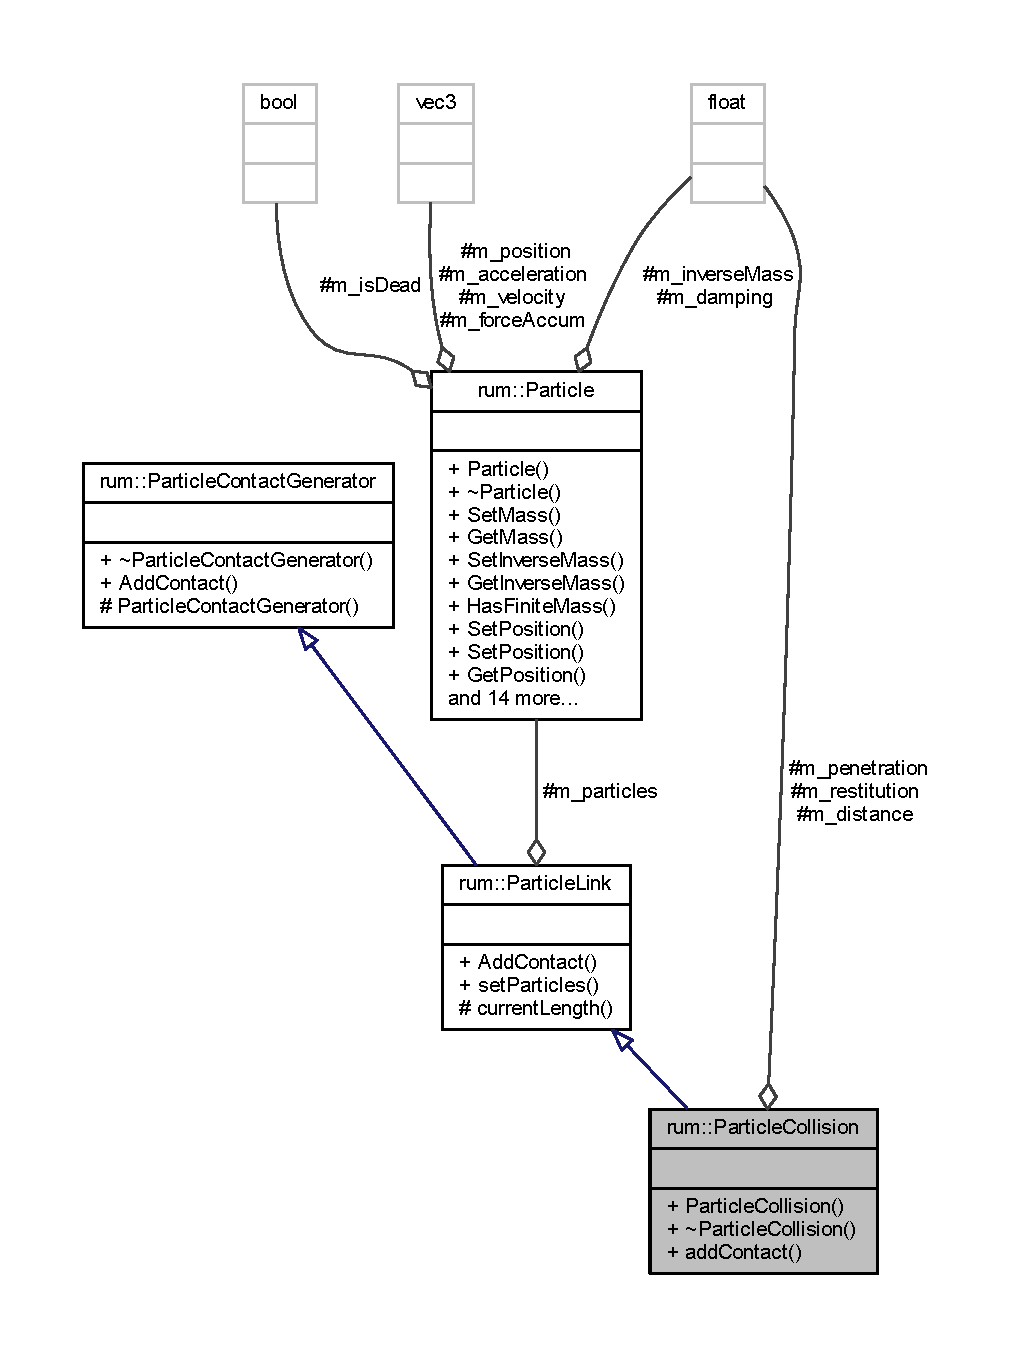
\includegraphics[width=350pt]{classrum_1_1_particle_collision__coll__graph}
\end{center}
\end{figure}
\subsection*{Public Member Functions}
\begin{DoxyCompactItemize}
\item 
\mbox{\hyperlink{classrum_1_1_particle_collision_a56570896eab4c089fd3df8fa6e96454c}{Particle\+Collision}} (\mbox{\hyperlink{namespacerum_a7e8cca23573d5eaead0f138cbaa4862c}{real}} restitution, \mbox{\hyperlink{namespacerum_a7e8cca23573d5eaead0f138cbaa4862c}{real}} distance, \mbox{\hyperlink{namespacerum_a7e8cca23573d5eaead0f138cbaa4862c}{real}} penetration)
\item 
\mbox{\hyperlink{classrum_1_1_particle_collision_afad930c6a0755e28c2bbca80cc7b5759}{$\sim$\+Particle\+Collision}} ()
\item 
unsigned int \mbox{\hyperlink{classrum_1_1_particle_collision_a0f935f8f4093623ea52a6fcbb902b2a4}{add\+Contact}} (\mbox{\hyperlink{classrum_1_1_particle_contact}{Particle\+Contact}} $\ast$contact, unsigned limit) const override
\end{DoxyCompactItemize}
\subsection*{Protected Attributes}
\begin{DoxyCompactItemize}
\item 
\mbox{\hyperlink{namespacerum_a7e8cca23573d5eaead0f138cbaa4862c}{real}} \mbox{\hyperlink{classrum_1_1_particle_collision_ae7aca9af657f5aea5e5e8c1261a51569}{m\+\_\+restitution}}
\item 
\mbox{\hyperlink{namespacerum_a7e8cca23573d5eaead0f138cbaa4862c}{real}} \mbox{\hyperlink{classrum_1_1_particle_collision_ae3b3e58675e2312ed3fe6a53c5882cc6}{m\+\_\+distance}}
\item 
\mbox{\hyperlink{namespacerum_a7e8cca23573d5eaead0f138cbaa4862c}{real}} \mbox{\hyperlink{classrum_1_1_particle_collision_a9ad398fd1a7b78e8ae8083610be60abb}{m\+\_\+penetration}}
\end{DoxyCompactItemize}
\subsection*{Additional Inherited Members}


\subsection{Constructor \& Destructor Documentation}
\mbox{\Hypertarget{classrum_1_1_particle_collision_a56570896eab4c089fd3df8fa6e96454c}\label{classrum_1_1_particle_collision_a56570896eab4c089fd3df8fa6e96454c}} 
\index{rum\+::\+Particle\+Collision@{rum\+::\+Particle\+Collision}!Particle\+Collision@{Particle\+Collision}}
\index{Particle\+Collision@{Particle\+Collision}!rum\+::\+Particle\+Collision@{rum\+::\+Particle\+Collision}}
\subsubsection{\texorpdfstring{Particle\+Collision()}{ParticleCollision()}}
{\footnotesize\ttfamily rum\+::\+Particle\+Collision\+::\+Particle\+Collision (\begin{DoxyParamCaption}\item[{\mbox{\hyperlink{namespacerum_a7e8cca23573d5eaead0f138cbaa4862c}{real}}}]{restitution,  }\item[{\mbox{\hyperlink{namespacerum_a7e8cca23573d5eaead0f138cbaa4862c}{real}}}]{distance,  }\item[{\mbox{\hyperlink{namespacerum_a7e8cca23573d5eaead0f138cbaa4862c}{real}}}]{penetration }\end{DoxyParamCaption})\hspace{0.3cm}{\ttfamily [explicit]}}

\mbox{\Hypertarget{classrum_1_1_particle_collision_afad930c6a0755e28c2bbca80cc7b5759}\label{classrum_1_1_particle_collision_afad930c6a0755e28c2bbca80cc7b5759}} 
\index{rum\+::\+Particle\+Collision@{rum\+::\+Particle\+Collision}!````~Particle\+Collision@{$\sim$\+Particle\+Collision}}
\index{````~Particle\+Collision@{$\sim$\+Particle\+Collision}!rum\+::\+Particle\+Collision@{rum\+::\+Particle\+Collision}}
\subsubsection{\texorpdfstring{$\sim$\+Particle\+Collision()}{~ParticleCollision()}}
{\footnotesize\ttfamily rum\+::\+Particle\+Collision\+::$\sim$\+Particle\+Collision (\begin{DoxyParamCaption}{ }\end{DoxyParamCaption})}



\subsection{Member Function Documentation}
\mbox{\Hypertarget{classrum_1_1_particle_collision_a0f935f8f4093623ea52a6fcbb902b2a4}\label{classrum_1_1_particle_collision_a0f935f8f4093623ea52a6fcbb902b2a4}} 
\index{rum\+::\+Particle\+Collision@{rum\+::\+Particle\+Collision}!add\+Contact@{add\+Contact}}
\index{add\+Contact@{add\+Contact}!rum\+::\+Particle\+Collision@{rum\+::\+Particle\+Collision}}
\subsubsection{\texorpdfstring{add\+Contact()}{addContact()}}
{\footnotesize\ttfamily unsigned int rum\+::\+Particle\+Collision\+::add\+Contact (\begin{DoxyParamCaption}\item[{\mbox{\hyperlink{classrum_1_1_particle_contact}{Particle\+Contact}} $\ast$}]{contact,  }\item[{unsigned}]{limit }\end{DoxyParamCaption}) const\hspace{0.3cm}{\ttfamily [override]}}



\subsection{Member Data Documentation}
\mbox{\Hypertarget{classrum_1_1_particle_collision_ae3b3e58675e2312ed3fe6a53c5882cc6}\label{classrum_1_1_particle_collision_ae3b3e58675e2312ed3fe6a53c5882cc6}} 
\index{rum\+::\+Particle\+Collision@{rum\+::\+Particle\+Collision}!m\+\_\+distance@{m\+\_\+distance}}
\index{m\+\_\+distance@{m\+\_\+distance}!rum\+::\+Particle\+Collision@{rum\+::\+Particle\+Collision}}
\subsubsection{\texorpdfstring{m\+\_\+distance}{m\_distance}}
{\footnotesize\ttfamily \mbox{\hyperlink{namespacerum_a7e8cca23573d5eaead0f138cbaa4862c}{real}} rum\+::\+Particle\+Collision\+::m\+\_\+distance\hspace{0.3cm}{\ttfamily [protected]}}

\mbox{\Hypertarget{classrum_1_1_particle_collision_a9ad398fd1a7b78e8ae8083610be60abb}\label{classrum_1_1_particle_collision_a9ad398fd1a7b78e8ae8083610be60abb}} 
\index{rum\+::\+Particle\+Collision@{rum\+::\+Particle\+Collision}!m\+\_\+penetration@{m\+\_\+penetration}}
\index{m\+\_\+penetration@{m\+\_\+penetration}!rum\+::\+Particle\+Collision@{rum\+::\+Particle\+Collision}}
\subsubsection{\texorpdfstring{m\+\_\+penetration}{m\_penetration}}
{\footnotesize\ttfamily \mbox{\hyperlink{namespacerum_a7e8cca23573d5eaead0f138cbaa4862c}{real}} rum\+::\+Particle\+Collision\+::m\+\_\+penetration\hspace{0.3cm}{\ttfamily [protected]}}

\mbox{\Hypertarget{classrum_1_1_particle_collision_ae7aca9af657f5aea5e5e8c1261a51569}\label{classrum_1_1_particle_collision_ae7aca9af657f5aea5e5e8c1261a51569}} 
\index{rum\+::\+Particle\+Collision@{rum\+::\+Particle\+Collision}!m\+\_\+restitution@{m\+\_\+restitution}}
\index{m\+\_\+restitution@{m\+\_\+restitution}!rum\+::\+Particle\+Collision@{rum\+::\+Particle\+Collision}}
\subsubsection{\texorpdfstring{m\+\_\+restitution}{m\_restitution}}
{\footnotesize\ttfamily \mbox{\hyperlink{namespacerum_a7e8cca23573d5eaead0f138cbaa4862c}{real}} rum\+::\+Particle\+Collision\+::m\+\_\+restitution\hspace{0.3cm}{\ttfamily [protected]}}



The documentation for this class was generated from the following files\+:\begin{DoxyCompactItemize}
\item 
D\+:/\+Library/\+Documents/\+Job/\+Forschungsmaster/\+Projekte/\+Rumble3\+D/\+Rumble3\+D/include/\+R3\+D/\+Particle\+Engine/\mbox{\hyperlink{_particle_collision_8h}{Particle\+Collision.\+h}}\item 
D\+:/\+Library/\+Documents/\+Job/\+Forschungsmaster/\+Projekte/\+Rumble3\+D/\+Rumble3\+D/src/\+Particle\+Engine/\mbox{\hyperlink{_particle_collision_8cpp}{Particle\+Collision.\+cpp}}\end{DoxyCompactItemize}

\hypertarget{classrum_1_1_particle_constraint}{}\section{rum\+:\+:Particle\+Constraint Class Reference}
\label{classrum_1_1_particle_constraint}\index{rum\+::\+Particle\+Constraint@{rum\+::\+Particle\+Constraint}}


{\ttfamily \#include $<$Particle\+Constraint.\+h$>$}



Inheritance diagram for rum\+:\+:Particle\+Constraint\+:\nopagebreak
\begin{figure}[H]
\begin{center}
\leavevmode
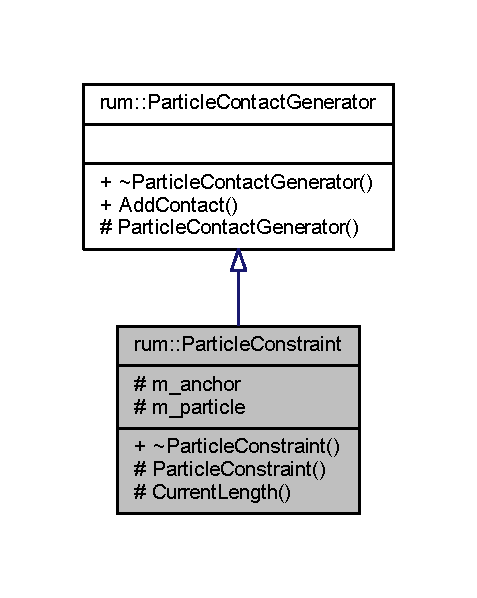
\includegraphics[width=229pt]{classrum_1_1_particle_constraint__inherit__graph}
\end{center}
\end{figure}


Collaboration diagram for rum\+:\+:Particle\+Constraint\+:\nopagebreak
\begin{figure}[H]
\begin{center}
\leavevmode
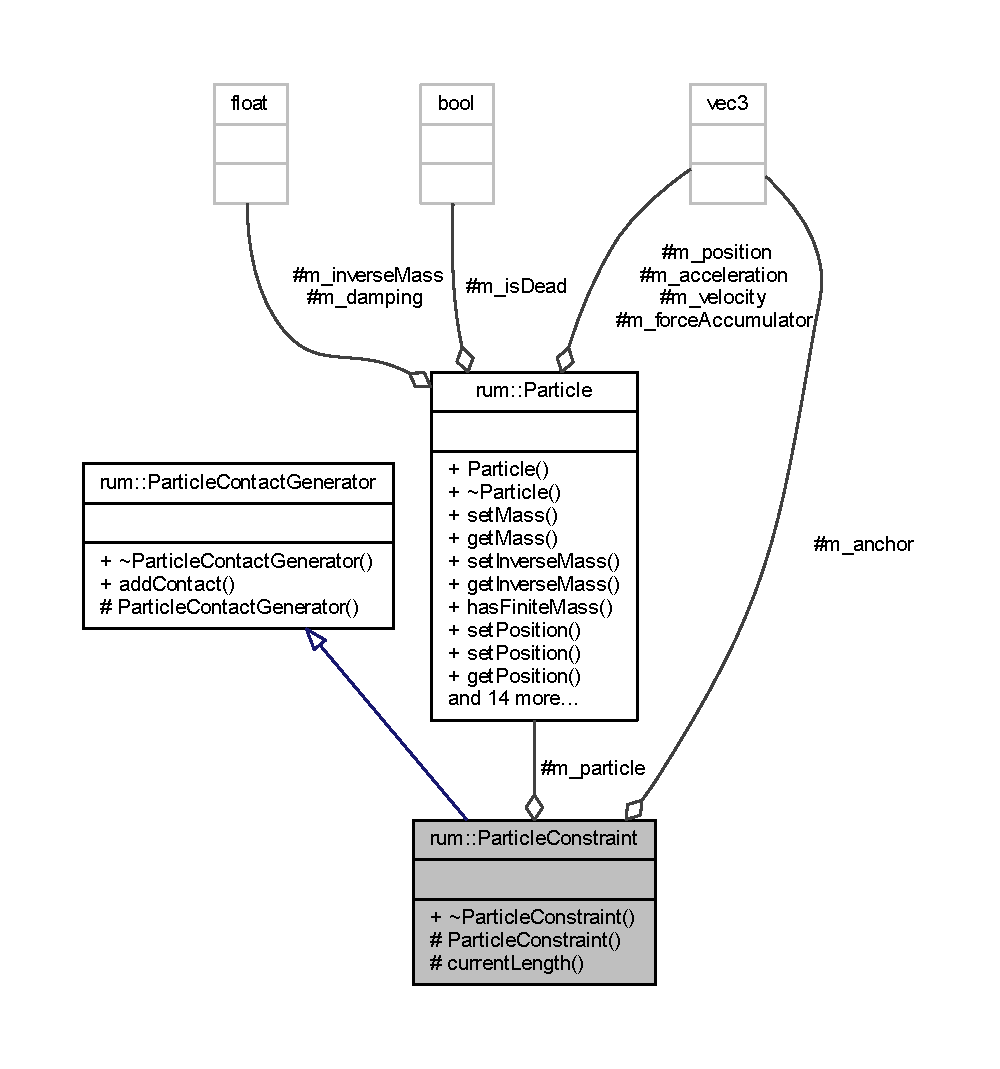
\includegraphics[width=350pt]{classrum_1_1_particle_constraint__coll__graph}
\end{center}
\end{figure}
\subsection*{Public Member Functions}
\begin{DoxyCompactItemize}
\item 
virtual \mbox{\hyperlink{classrum_1_1_particle_constraint_a746b1856af604ddc7e0b763114b11d43}{$\sim$\+Particle\+Constraint}} ()
\end{DoxyCompactItemize}
\subsection*{Protected Member Functions}
\begin{DoxyCompactItemize}
\item 
\mbox{\hyperlink{classrum_1_1_particle_constraint_aee5151f3813c45df9e65bf5ae29ba1d1}{Particle\+Constraint}} ()
\item 
\mbox{\hyperlink{namespacerum_a7e8cca23573d5eaead0f138cbaa4862c}{real}} \mbox{\hyperlink{classrum_1_1_particle_constraint_a5a9d5520ee68acb19f91b792c0858d1d}{current\+Length}} () const
\end{DoxyCompactItemize}
\subsection*{Protected Attributes}
\begin{DoxyCompactItemize}
\item 
glm\+::vec3 \mbox{\hyperlink{classrum_1_1_particle_constraint_a9822cd4e0be33424d7b3ffe0dce583a8}{m\+\_\+anchor}}
\item 
\mbox{\hyperlink{classrum_1_1_particle}{Particle}} $\ast$ \mbox{\hyperlink{classrum_1_1_particle_constraint_a78a37fb2e7d93ebdace6020a484ab35e}{m\+\_\+particle}}
\end{DoxyCompactItemize}


\subsection{Constructor \& Destructor Documentation}
\mbox{\Hypertarget{classrum_1_1_particle_constraint_a746b1856af604ddc7e0b763114b11d43}\label{classrum_1_1_particle_constraint_a746b1856af604ddc7e0b763114b11d43}} 
\index{rum\+::\+Particle\+Constraint@{rum\+::\+Particle\+Constraint}!````~Particle\+Constraint@{$\sim$\+Particle\+Constraint}}
\index{````~Particle\+Constraint@{$\sim$\+Particle\+Constraint}!rum\+::\+Particle\+Constraint@{rum\+::\+Particle\+Constraint}}
\subsubsection{\texorpdfstring{$\sim$\+Particle\+Constraint()}{~ParticleConstraint()}}
{\footnotesize\ttfamily rum\+::\+Particle\+Constraint\+::$\sim$\+Particle\+Constraint (\begin{DoxyParamCaption}{ }\end{DoxyParamCaption})\hspace{0.3cm}{\ttfamily [virtual]}}

\mbox{\Hypertarget{classrum_1_1_particle_constraint_aee5151f3813c45df9e65bf5ae29ba1d1}\label{classrum_1_1_particle_constraint_aee5151f3813c45df9e65bf5ae29ba1d1}} 
\index{rum\+::\+Particle\+Constraint@{rum\+::\+Particle\+Constraint}!Particle\+Constraint@{Particle\+Constraint}}
\index{Particle\+Constraint@{Particle\+Constraint}!rum\+::\+Particle\+Constraint@{rum\+::\+Particle\+Constraint}}
\subsubsection{\texorpdfstring{Particle\+Constraint()}{ParticleConstraint()}}
{\footnotesize\ttfamily rum\+::\+Particle\+Constraint\+::\+Particle\+Constraint (\begin{DoxyParamCaption}{ }\end{DoxyParamCaption})\hspace{0.3cm}{\ttfamily [explicit]}, {\ttfamily [protected]}}



\subsection{Member Function Documentation}
\mbox{\Hypertarget{classrum_1_1_particle_constraint_a5a9d5520ee68acb19f91b792c0858d1d}\label{classrum_1_1_particle_constraint_a5a9d5520ee68acb19f91b792c0858d1d}} 
\index{rum\+::\+Particle\+Constraint@{rum\+::\+Particle\+Constraint}!current\+Length@{current\+Length}}
\index{current\+Length@{current\+Length}!rum\+::\+Particle\+Constraint@{rum\+::\+Particle\+Constraint}}
\subsubsection{\texorpdfstring{current\+Length()}{currentLength()}}
{\footnotesize\ttfamily \mbox{\hyperlink{namespacerum_a7e8cca23573d5eaead0f138cbaa4862c}{real}} rum\+::\+Particle\+Constraint\+::current\+Length (\begin{DoxyParamCaption}{ }\end{DoxyParamCaption}) const\hspace{0.3cm}{\ttfamily [protected]}}



\subsection{Member Data Documentation}
\mbox{\Hypertarget{classrum_1_1_particle_constraint_a9822cd4e0be33424d7b3ffe0dce583a8}\label{classrum_1_1_particle_constraint_a9822cd4e0be33424d7b3ffe0dce583a8}} 
\index{rum\+::\+Particle\+Constraint@{rum\+::\+Particle\+Constraint}!m\+\_\+anchor@{m\+\_\+anchor}}
\index{m\+\_\+anchor@{m\+\_\+anchor}!rum\+::\+Particle\+Constraint@{rum\+::\+Particle\+Constraint}}
\subsubsection{\texorpdfstring{m\+\_\+anchor}{m\_anchor}}
{\footnotesize\ttfamily glm\+::vec3 rum\+::\+Particle\+Constraint\+::m\+\_\+anchor\hspace{0.3cm}{\ttfamily [protected]}}

\mbox{\Hypertarget{classrum_1_1_particle_constraint_a78a37fb2e7d93ebdace6020a484ab35e}\label{classrum_1_1_particle_constraint_a78a37fb2e7d93ebdace6020a484ab35e}} 
\index{rum\+::\+Particle\+Constraint@{rum\+::\+Particle\+Constraint}!m\+\_\+particle@{m\+\_\+particle}}
\index{m\+\_\+particle@{m\+\_\+particle}!rum\+::\+Particle\+Constraint@{rum\+::\+Particle\+Constraint}}
\subsubsection{\texorpdfstring{m\+\_\+particle}{m\_particle}}
{\footnotesize\ttfamily \mbox{\hyperlink{classrum_1_1_particle}{Particle}}$\ast$ rum\+::\+Particle\+Constraint\+::m\+\_\+particle\hspace{0.3cm}{\ttfamily [protected]}}



The documentation for this class was generated from the following files\+:\begin{DoxyCompactItemize}
\item 
D\+:/\+Library/\+Documents/\+Job/\+Forschungsmaster/\+Projekte/\+Rumble3\+D/\+Rumble3\+D/include/\+R3\+D/\+Particle\+Engine/\mbox{\hyperlink{_particle_constraint_8h}{Particle\+Constraint.\+h}}\item 
D\+:/\+Library/\+Documents/\+Job/\+Forschungsmaster/\+Projekte/\+Rumble3\+D/\+Rumble3\+D/src/\+Particle\+Engine/\mbox{\hyperlink{_particle_constraint_8cpp}{Particle\+Constraint.\+cpp}}\end{DoxyCompactItemize}

\hypertarget{classrum_1_1_particle_contact}{}\section{rum\+:\+:Particle\+Contact Class Reference}
\label{classrum_1_1_particle_contact}\index{rum\+::\+Particle\+Contact@{rum\+::\+Particle\+Contact}}


{\ttfamily \#include $<$Particle\+Contact.\+h$>$}



Collaboration diagram for rum\+:\+:Particle\+Contact\+:\nopagebreak
\begin{figure}[H]
\begin{center}
\leavevmode
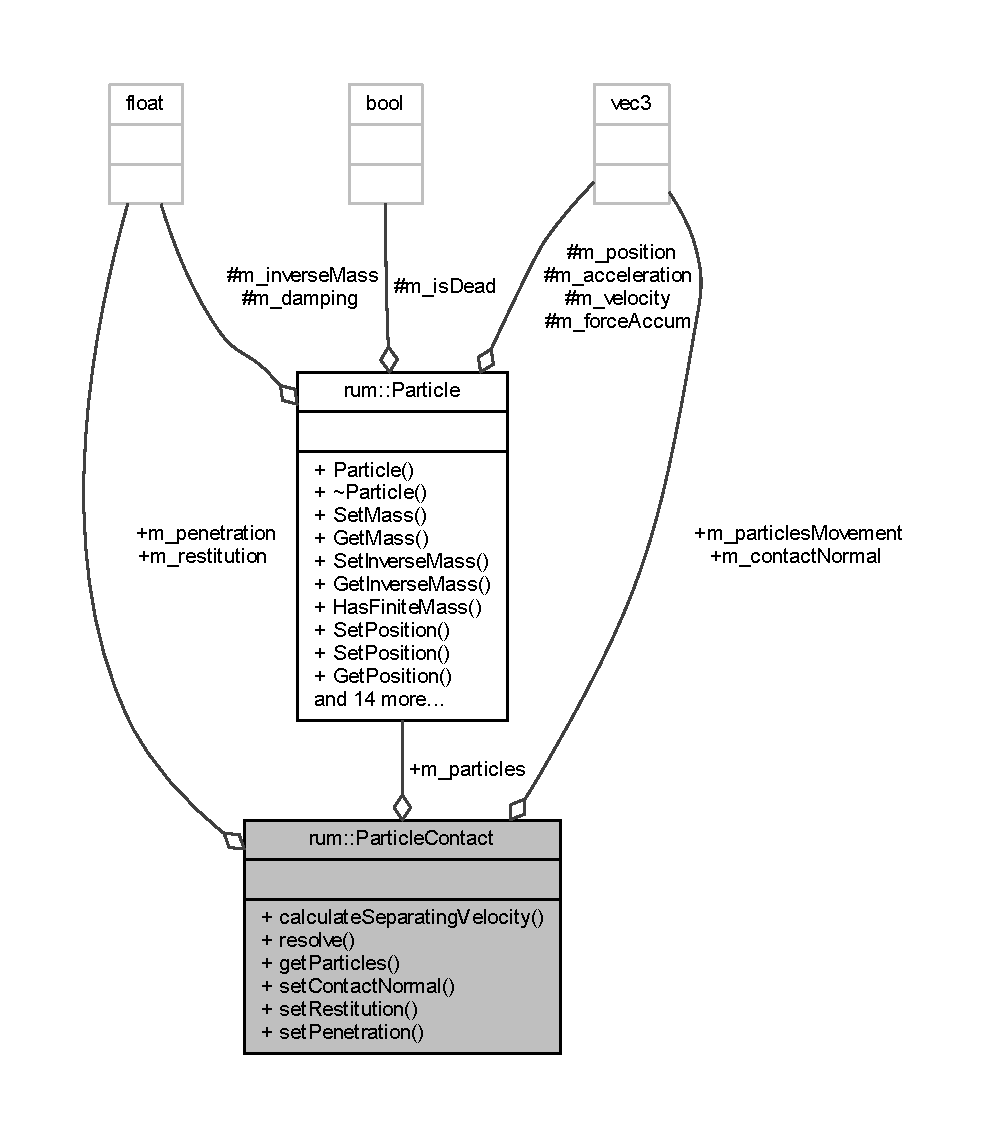
\includegraphics[width=350pt]{classrum_1_1_particle_contact__coll__graph}
\end{center}
\end{figure}
\subsection*{Public Member Functions}
\begin{DoxyCompactItemize}
\item 
\mbox{\hyperlink{classrum_1_1_particle_contact_aab189df2f191ed165769f7545c0681d9}{Particle\+Contact}} ()
\item 
\mbox{\hyperlink{classrum_1_1_particle_contact_aa1f7ccaa9ef517fae352e24a9bc8e79e}{$\sim$\+Particle\+Contact}} ()
\item 
\mbox{\hyperlink{namespacerum_a7e8cca23573d5eaead0f138cbaa4862c}{real}} \mbox{\hyperlink{classrum_1_1_particle_contact_a85e06dde6b23622bf8d9f6a99205fcfc}{calculate\+Separating\+Velocity}} () const
\item 
void \mbox{\hyperlink{classrum_1_1_particle_contact_acf090d7537e78bea0e9008b55a3959c9}{resolve}} (\mbox{\hyperlink{namespacerum_a7e8cca23573d5eaead0f138cbaa4862c}{real}} duration)
\item 
\mbox{\hyperlink{classrum_1_1_particle}{Particle}} $\ast$ \mbox{\hyperlink{classrum_1_1_particle_contact_a3cccc345ae55939b5fca963e86d7deae}{get\+Particles}} ()
\item 
void \mbox{\hyperlink{classrum_1_1_particle_contact_a0626aa815eab861f15cc9dfc582452a6}{set\+Contact\+Normal}} (glm\+::vec3 normal)
\item 
void \mbox{\hyperlink{classrum_1_1_particle_contact_abf356cecb0c3c42d889a561afc901a97}{set\+Restitution}} (\mbox{\hyperlink{namespacerum_a7e8cca23573d5eaead0f138cbaa4862c}{real}} restitution)
\item 
void \mbox{\hyperlink{classrum_1_1_particle_contact_ab31f404b4e571262ade5c9d8b1f36f97}{set\+Penetration}} (\mbox{\hyperlink{namespacerum_a7e8cca23573d5eaead0f138cbaa4862c}{real}} penetration)
\end{DoxyCompactItemize}
\subsection*{Public Attributes}
\begin{DoxyCompactItemize}
\item 
\mbox{\hyperlink{classrum_1_1_particle}{Particle}} $\ast$ \mbox{\hyperlink{classrum_1_1_particle_contact_a01267c3d6f9227b318a7b49182d01006}{m\+\_\+particles}} \mbox{[}2\mbox{]} \{\}
\item 
\mbox{\hyperlink{namespacerum_a7e8cca23573d5eaead0f138cbaa4862c}{real}} \mbox{\hyperlink{classrum_1_1_particle_contact_a0be16bc823ae27866228345eb3349482}{m\+\_\+restitution}} \{\}
\item 
glm\+::vec3 \mbox{\hyperlink{classrum_1_1_particle_contact_a8b0d26e0c773a739f34eb27d7e8d9c17}{m\+\_\+contact\+Normal}}
\item 
\mbox{\hyperlink{namespacerum_a7e8cca23573d5eaead0f138cbaa4862c}{real}} \mbox{\hyperlink{classrum_1_1_particle_contact_a935966849508ec47d3c6330816f873de}{m\+\_\+penetration}} \{\}
\item 
glm\+::vec3 \mbox{\hyperlink{classrum_1_1_particle_contact_ab03921d708387e5bbc3a0c01f1f5a3da}{m\+\_\+particles\+Movement}} \mbox{[}2\mbox{]}
\end{DoxyCompactItemize}
\subsection*{Friends}
\begin{DoxyCompactItemize}
\item 
class \mbox{\hyperlink{classrum_1_1_particle_contact_ab2e3f4c3dc9b46966c6ec90e0fe88b6c}{Particle\+Contact\+Resolver}}
\end{DoxyCompactItemize}


\subsection{Constructor \& Destructor Documentation}
\mbox{\Hypertarget{classrum_1_1_particle_contact_aab189df2f191ed165769f7545c0681d9}\label{classrum_1_1_particle_contact_aab189df2f191ed165769f7545c0681d9}} 
\index{rum\+::\+Particle\+Contact@{rum\+::\+Particle\+Contact}!Particle\+Contact@{Particle\+Contact}}
\index{Particle\+Contact@{Particle\+Contact}!rum\+::\+Particle\+Contact@{rum\+::\+Particle\+Contact}}
\subsubsection{\texorpdfstring{Particle\+Contact()}{ParticleContact()}}
{\footnotesize\ttfamily rum\+::\+Particle\+Contact\+::\+Particle\+Contact (\begin{DoxyParamCaption}{ }\end{DoxyParamCaption})\hspace{0.3cm}{\ttfamily [explicit]}, {\ttfamily [default]}}

\mbox{\Hypertarget{classrum_1_1_particle_contact_aa1f7ccaa9ef517fae352e24a9bc8e79e}\label{classrum_1_1_particle_contact_aa1f7ccaa9ef517fae352e24a9bc8e79e}} 
\index{rum\+::\+Particle\+Contact@{rum\+::\+Particle\+Contact}!````~Particle\+Contact@{$\sim$\+Particle\+Contact}}
\index{````~Particle\+Contact@{$\sim$\+Particle\+Contact}!rum\+::\+Particle\+Contact@{rum\+::\+Particle\+Contact}}
\subsubsection{\texorpdfstring{$\sim$\+Particle\+Contact()}{~ParticleContact()}}
{\footnotesize\ttfamily rum\+::\+Particle\+Contact\+::$\sim$\+Particle\+Contact (\begin{DoxyParamCaption}{ }\end{DoxyParamCaption})\hspace{0.3cm}{\ttfamily [default]}}



\subsection{Member Function Documentation}
\mbox{\Hypertarget{classrum_1_1_particle_contact_a85e06dde6b23622bf8d9f6a99205fcfc}\label{classrum_1_1_particle_contact_a85e06dde6b23622bf8d9f6a99205fcfc}} 
\index{rum\+::\+Particle\+Contact@{rum\+::\+Particle\+Contact}!calculate\+Separating\+Velocity@{calculate\+Separating\+Velocity}}
\index{calculate\+Separating\+Velocity@{calculate\+Separating\+Velocity}!rum\+::\+Particle\+Contact@{rum\+::\+Particle\+Contact}}
\subsubsection{\texorpdfstring{calculate\+Separating\+Velocity()}{calculateSeparatingVelocity()}}
{\footnotesize\ttfamily \mbox{\hyperlink{namespacerum_a7e8cca23573d5eaead0f138cbaa4862c}{real}} rum\+::\+Particle\+Contact\+::calculate\+Separating\+Velocity (\begin{DoxyParamCaption}{ }\end{DoxyParamCaption}) const}

\mbox{\Hypertarget{classrum_1_1_particle_contact_a3cccc345ae55939b5fca963e86d7deae}\label{classrum_1_1_particle_contact_a3cccc345ae55939b5fca963e86d7deae}} 
\index{rum\+::\+Particle\+Contact@{rum\+::\+Particle\+Contact}!get\+Particles@{get\+Particles}}
\index{get\+Particles@{get\+Particles}!rum\+::\+Particle\+Contact@{rum\+::\+Particle\+Contact}}
\subsubsection{\texorpdfstring{get\+Particles()}{getParticles()}}
{\footnotesize\ttfamily \mbox{\hyperlink{classrum_1_1_particle}{Particle}} $\ast$ rum\+::\+Particle\+Contact\+::get\+Particles (\begin{DoxyParamCaption}{ }\end{DoxyParamCaption})}

\mbox{\Hypertarget{classrum_1_1_particle_contact_acf090d7537e78bea0e9008b55a3959c9}\label{classrum_1_1_particle_contact_acf090d7537e78bea0e9008b55a3959c9}} 
\index{rum\+::\+Particle\+Contact@{rum\+::\+Particle\+Contact}!resolve@{resolve}}
\index{resolve@{resolve}!rum\+::\+Particle\+Contact@{rum\+::\+Particle\+Contact}}
\subsubsection{\texorpdfstring{resolve()}{resolve()}}
{\footnotesize\ttfamily void rum\+::\+Particle\+Contact\+::resolve (\begin{DoxyParamCaption}\item[{\mbox{\hyperlink{namespacerum_a7e8cca23573d5eaead0f138cbaa4862c}{real}}}]{duration }\end{DoxyParamCaption})}

\mbox{\Hypertarget{classrum_1_1_particle_contact_a0626aa815eab861f15cc9dfc582452a6}\label{classrum_1_1_particle_contact_a0626aa815eab861f15cc9dfc582452a6}} 
\index{rum\+::\+Particle\+Contact@{rum\+::\+Particle\+Contact}!set\+Contact\+Normal@{set\+Contact\+Normal}}
\index{set\+Contact\+Normal@{set\+Contact\+Normal}!rum\+::\+Particle\+Contact@{rum\+::\+Particle\+Contact}}
\subsubsection{\texorpdfstring{set\+Contact\+Normal()}{setContactNormal()}}
{\footnotesize\ttfamily void rum\+::\+Particle\+Contact\+::set\+Contact\+Normal (\begin{DoxyParamCaption}\item[{glm\+::vec3}]{normal }\end{DoxyParamCaption})}

\mbox{\Hypertarget{classrum_1_1_particle_contact_ab31f404b4e571262ade5c9d8b1f36f97}\label{classrum_1_1_particle_contact_ab31f404b4e571262ade5c9d8b1f36f97}} 
\index{rum\+::\+Particle\+Contact@{rum\+::\+Particle\+Contact}!set\+Penetration@{set\+Penetration}}
\index{set\+Penetration@{set\+Penetration}!rum\+::\+Particle\+Contact@{rum\+::\+Particle\+Contact}}
\subsubsection{\texorpdfstring{set\+Penetration()}{setPenetration()}}
{\footnotesize\ttfamily void rum\+::\+Particle\+Contact\+::set\+Penetration (\begin{DoxyParamCaption}\item[{\mbox{\hyperlink{namespacerum_a7e8cca23573d5eaead0f138cbaa4862c}{real}}}]{penetration }\end{DoxyParamCaption})}

\mbox{\Hypertarget{classrum_1_1_particle_contact_abf356cecb0c3c42d889a561afc901a97}\label{classrum_1_1_particle_contact_abf356cecb0c3c42d889a561afc901a97}} 
\index{rum\+::\+Particle\+Contact@{rum\+::\+Particle\+Contact}!set\+Restitution@{set\+Restitution}}
\index{set\+Restitution@{set\+Restitution}!rum\+::\+Particle\+Contact@{rum\+::\+Particle\+Contact}}
\subsubsection{\texorpdfstring{set\+Restitution()}{setRestitution()}}
{\footnotesize\ttfamily void rum\+::\+Particle\+Contact\+::set\+Restitution (\begin{DoxyParamCaption}\item[{\mbox{\hyperlink{namespacerum_a7e8cca23573d5eaead0f138cbaa4862c}{real}}}]{restitution }\end{DoxyParamCaption})}



\subsection{Friends And Related Function Documentation}
\mbox{\Hypertarget{classrum_1_1_particle_contact_ab2e3f4c3dc9b46966c6ec90e0fe88b6c}\label{classrum_1_1_particle_contact_ab2e3f4c3dc9b46966c6ec90e0fe88b6c}} 
\index{rum\+::\+Particle\+Contact@{rum\+::\+Particle\+Contact}!Particle\+Contact\+Resolver@{Particle\+Contact\+Resolver}}
\index{Particle\+Contact\+Resolver@{Particle\+Contact\+Resolver}!rum\+::\+Particle\+Contact@{rum\+::\+Particle\+Contact}}
\subsubsection{\texorpdfstring{Particle\+Contact\+Resolver}{ParticleContactResolver}}
{\footnotesize\ttfamily friend class \mbox{\hyperlink{classrum_1_1_particle_contact_resolver}{Particle\+Contact\+Resolver}}\hspace{0.3cm}{\ttfamily [friend]}}



\subsection{Member Data Documentation}
\mbox{\Hypertarget{classrum_1_1_particle_contact_a8b0d26e0c773a739f34eb27d7e8d9c17}\label{classrum_1_1_particle_contact_a8b0d26e0c773a739f34eb27d7e8d9c17}} 
\index{rum\+::\+Particle\+Contact@{rum\+::\+Particle\+Contact}!m\+\_\+contact\+Normal@{m\+\_\+contact\+Normal}}
\index{m\+\_\+contact\+Normal@{m\+\_\+contact\+Normal}!rum\+::\+Particle\+Contact@{rum\+::\+Particle\+Contact}}
\subsubsection{\texorpdfstring{m\+\_\+contact\+Normal}{m\_contactNormal}}
{\footnotesize\ttfamily glm\+::vec3 rum\+::\+Particle\+Contact\+::m\+\_\+contact\+Normal}

\mbox{\Hypertarget{classrum_1_1_particle_contact_a01267c3d6f9227b318a7b49182d01006}\label{classrum_1_1_particle_contact_a01267c3d6f9227b318a7b49182d01006}} 
\index{rum\+::\+Particle\+Contact@{rum\+::\+Particle\+Contact}!m\+\_\+particles@{m\+\_\+particles}}
\index{m\+\_\+particles@{m\+\_\+particles}!rum\+::\+Particle\+Contact@{rum\+::\+Particle\+Contact}}
\subsubsection{\texorpdfstring{m\+\_\+particles}{m\_particles}}
{\footnotesize\ttfamily \mbox{\hyperlink{classrum_1_1_particle}{Particle}}$\ast$ rum\+::\+Particle\+Contact\+::m\+\_\+particles\mbox{[}2\mbox{]} \{\}}

\mbox{\Hypertarget{classrum_1_1_particle_contact_ab03921d708387e5bbc3a0c01f1f5a3da}\label{classrum_1_1_particle_contact_ab03921d708387e5bbc3a0c01f1f5a3da}} 
\index{rum\+::\+Particle\+Contact@{rum\+::\+Particle\+Contact}!m\+\_\+particles\+Movement@{m\+\_\+particles\+Movement}}
\index{m\+\_\+particles\+Movement@{m\+\_\+particles\+Movement}!rum\+::\+Particle\+Contact@{rum\+::\+Particle\+Contact}}
\subsubsection{\texorpdfstring{m\+\_\+particles\+Movement}{m\_particlesMovement}}
{\footnotesize\ttfamily glm\+::vec3 rum\+::\+Particle\+Contact\+::m\+\_\+particles\+Movement\mbox{[}2\mbox{]}}

\mbox{\Hypertarget{classrum_1_1_particle_contact_a935966849508ec47d3c6330816f873de}\label{classrum_1_1_particle_contact_a935966849508ec47d3c6330816f873de}} 
\index{rum\+::\+Particle\+Contact@{rum\+::\+Particle\+Contact}!m\+\_\+penetration@{m\+\_\+penetration}}
\index{m\+\_\+penetration@{m\+\_\+penetration}!rum\+::\+Particle\+Contact@{rum\+::\+Particle\+Contact}}
\subsubsection{\texorpdfstring{m\+\_\+penetration}{m\_penetration}}
{\footnotesize\ttfamily \mbox{\hyperlink{namespacerum_a7e8cca23573d5eaead0f138cbaa4862c}{real}} rum\+::\+Particle\+Contact\+::m\+\_\+penetration \{\}}

\mbox{\Hypertarget{classrum_1_1_particle_contact_a0be16bc823ae27866228345eb3349482}\label{classrum_1_1_particle_contact_a0be16bc823ae27866228345eb3349482}} 
\index{rum\+::\+Particle\+Contact@{rum\+::\+Particle\+Contact}!m\+\_\+restitution@{m\+\_\+restitution}}
\index{m\+\_\+restitution@{m\+\_\+restitution}!rum\+::\+Particle\+Contact@{rum\+::\+Particle\+Contact}}
\subsubsection{\texorpdfstring{m\+\_\+restitution}{m\_restitution}}
{\footnotesize\ttfamily \mbox{\hyperlink{namespacerum_a7e8cca23573d5eaead0f138cbaa4862c}{real}} rum\+::\+Particle\+Contact\+::m\+\_\+restitution \{\}}



The documentation for this class was generated from the following files\+:\begin{DoxyCompactItemize}
\item 
D\+:/\+Library/\+Documents/\+Job/\+Forschungsmaster/\+Projekte/\+Rumble3\+D/\+Rumble3\+D/include/\+R3\+D/\+Particle\+Engine/\mbox{\hyperlink{_particle_contact_8h}{Particle\+Contact.\+h}}\item 
D\+:/\+Library/\+Documents/\+Job/\+Forschungsmaster/\+Projekte/\+Rumble3\+D/\+Rumble3\+D/src/\+Particle\+Engine/\mbox{\hyperlink{_particle_contact_8cpp}{Particle\+Contact.\+cpp}}\end{DoxyCompactItemize}

\hypertarget{classrum_1_1_particle_contact_generator}{}\section{rum\+:\+:Particle\+Contact\+Generator Class Reference}
\label{classrum_1_1_particle_contact_generator}\index{rum\+::\+Particle\+Contact\+Generator@{rum\+::\+Particle\+Contact\+Generator}}


{\ttfamily \#include $<$Particle\+Contact\+Generator.\+h$>$}



Inheritance diagram for rum\+:\+:Particle\+Contact\+Generator\+:\nopagebreak
\begin{figure}[H]
\begin{center}
\leavevmode
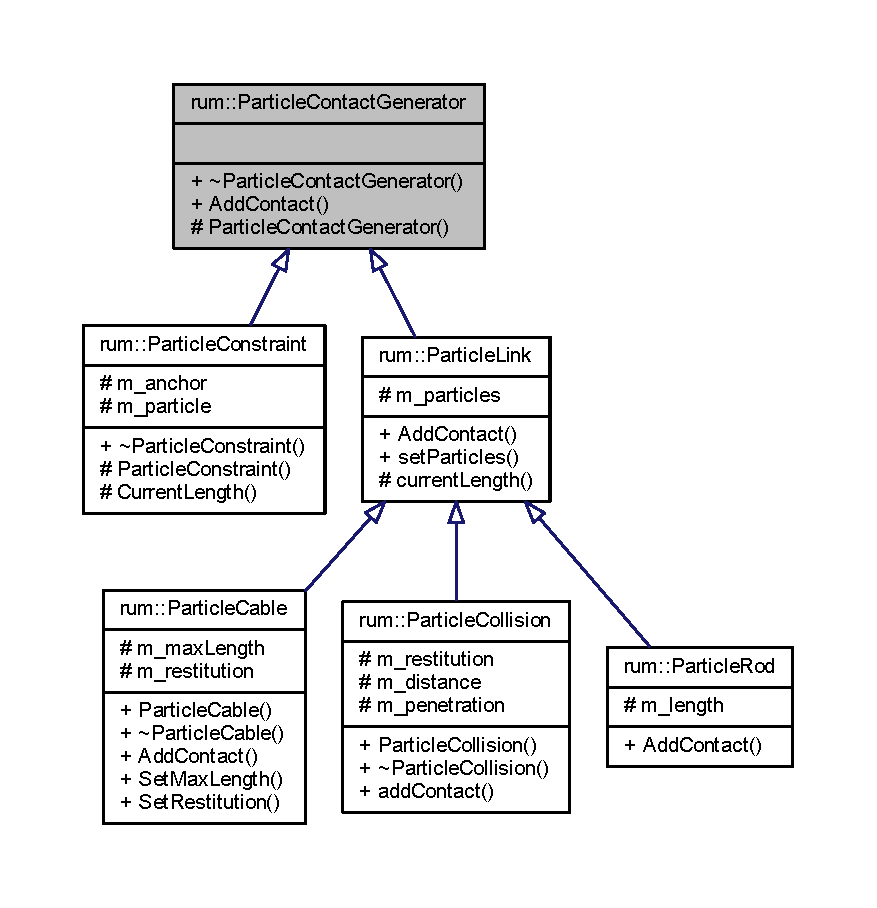
\includegraphics[width=350pt]{classrum_1_1_particle_contact_generator__inherit__graph}
\end{center}
\end{figure}


Collaboration diagram for rum\+:\+:Particle\+Contact\+Generator\+:\nopagebreak
\begin{figure}[H]
\begin{center}
\leavevmode
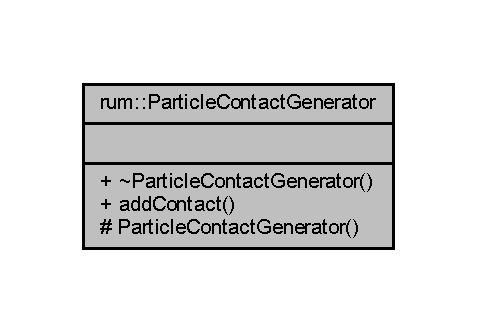
\includegraphics[width=229pt]{classrum_1_1_particle_contact_generator__coll__graph}
\end{center}
\end{figure}
\subsection*{Public Member Functions}
\begin{DoxyCompactItemize}
\item 
virtual \mbox{\hyperlink{classrum_1_1_particle_contact_generator_a79743de72e95cfa6db189bc9f0d99b71}{$\sim$\+Particle\+Contact\+Generator}} ()
\item 
virtual unsigned \mbox{\hyperlink{classrum_1_1_particle_contact_generator_a343d3df815d7e170458fe937fe82aad5}{add\+Contact}} (\mbox{\hyperlink{classrum_1_1_particle_contact}{Particle\+Contact}} $\ast$contact, unsigned int limit) const =0
\end{DoxyCompactItemize}
\subsection*{Protected Member Functions}
\begin{DoxyCompactItemize}
\item 
\mbox{\hyperlink{classrum_1_1_particle_contact_generator_aefec37ffef72a54397c6952c6d2e65ba}{Particle\+Contact\+Generator}} ()
\end{DoxyCompactItemize}


\subsection{Constructor \& Destructor Documentation}
\mbox{\Hypertarget{classrum_1_1_particle_contact_generator_a79743de72e95cfa6db189bc9f0d99b71}\label{classrum_1_1_particle_contact_generator_a79743de72e95cfa6db189bc9f0d99b71}} 
\index{rum\+::\+Particle\+Contact\+Generator@{rum\+::\+Particle\+Contact\+Generator}!````~Particle\+Contact\+Generator@{$\sim$\+Particle\+Contact\+Generator}}
\index{````~Particle\+Contact\+Generator@{$\sim$\+Particle\+Contact\+Generator}!rum\+::\+Particle\+Contact\+Generator@{rum\+::\+Particle\+Contact\+Generator}}
\subsubsection{\texorpdfstring{$\sim$\+Particle\+Contact\+Generator()}{~ParticleContactGenerator()}}
{\footnotesize\ttfamily rum\+::\+Particle\+Contact\+Generator\+::$\sim$\+Particle\+Contact\+Generator (\begin{DoxyParamCaption}{ }\end{DoxyParamCaption})\hspace{0.3cm}{\ttfamily [virtual]}}

\mbox{\Hypertarget{classrum_1_1_particle_contact_generator_aefec37ffef72a54397c6952c6d2e65ba}\label{classrum_1_1_particle_contact_generator_aefec37ffef72a54397c6952c6d2e65ba}} 
\index{rum\+::\+Particle\+Contact\+Generator@{rum\+::\+Particle\+Contact\+Generator}!Particle\+Contact\+Generator@{Particle\+Contact\+Generator}}
\index{Particle\+Contact\+Generator@{Particle\+Contact\+Generator}!rum\+::\+Particle\+Contact\+Generator@{rum\+::\+Particle\+Contact\+Generator}}
\subsubsection{\texorpdfstring{Particle\+Contact\+Generator()}{ParticleContactGenerator()}}
{\footnotesize\ttfamily rum\+::\+Particle\+Contact\+Generator\+::\+Particle\+Contact\+Generator (\begin{DoxyParamCaption}{ }\end{DoxyParamCaption})\hspace{0.3cm}{\ttfamily [explicit]}, {\ttfamily [protected]}}



\subsection{Member Function Documentation}
\mbox{\Hypertarget{classrum_1_1_particle_contact_generator_a343d3df815d7e170458fe937fe82aad5}\label{classrum_1_1_particle_contact_generator_a343d3df815d7e170458fe937fe82aad5}} 
\index{rum\+::\+Particle\+Contact\+Generator@{rum\+::\+Particle\+Contact\+Generator}!add\+Contact@{add\+Contact}}
\index{add\+Contact@{add\+Contact}!rum\+::\+Particle\+Contact\+Generator@{rum\+::\+Particle\+Contact\+Generator}}
\subsubsection{\texorpdfstring{add\+Contact()}{addContact()}}
{\footnotesize\ttfamily virtual unsigned rum\+::\+Particle\+Contact\+Generator\+::add\+Contact (\begin{DoxyParamCaption}\item[{\mbox{\hyperlink{classrum_1_1_particle_contact}{Particle\+Contact}} $\ast$}]{contact,  }\item[{unsigned int}]{limit }\end{DoxyParamCaption}) const\hspace{0.3cm}{\ttfamily [pure virtual]}}



Implemented in \mbox{\hyperlink{classrum_1_1_particle_link_a0da76619bd1d2ae04d5f8173c2883ff2}{rum\+::\+Particle\+Link}}, and \mbox{\hyperlink{classrum_1_1_particle_cable_a078344be0db7ccc00d326ac767736431}{rum\+::\+Particle\+Cable}}.



The documentation for this class was generated from the following files\+:\begin{DoxyCompactItemize}
\item 
D\+:/\+Library/\+Documents/\+Job/\+Forschungsmaster/\+Projekte/\+Rumble3\+D/\+Rumble3\+D/include/\+R3\+D/\+Particle\+Engine/\mbox{\hyperlink{_particle_contact_generator_8h}{Particle\+Contact\+Generator.\+h}}\item 
D\+:/\+Library/\+Documents/\+Job/\+Forschungsmaster/\+Projekte/\+Rumble3\+D/\+Rumble3\+D/src/\+Particle\+Engine/\mbox{\hyperlink{_particle_contact_generator_8cpp}{Particle\+Contact\+Generator.\+cpp}}\end{DoxyCompactItemize}

\hypertarget{classrum_1_1_particle_contact_resolver}{}\section{rum\+:\+:Particle\+Contact\+Resolver Class Reference}
\label{classrum_1_1_particle_contact_resolver}\index{rum\+::\+Particle\+Contact\+Resolver@{rum\+::\+Particle\+Contact\+Resolver}}


{\ttfamily \#include $<$Particle\+Contact\+Resolver.\+h$>$}



Collaboration diagram for rum\+:\+:Particle\+Contact\+Resolver\+:\nopagebreak
\begin{figure}[H]
\begin{center}
\leavevmode
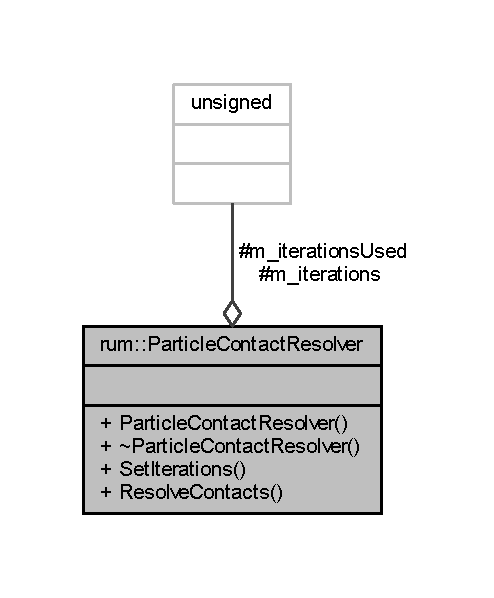
\includegraphics[width=237pt]{classrum_1_1_particle_contact_resolver__coll__graph}
\end{center}
\end{figure}
\subsection*{Public Member Functions}
\begin{DoxyCompactItemize}
\item 
\mbox{\hyperlink{classrum_1_1_particle_contact_resolver_a1921a5520c8940065d04f3bb890680bc}{Particle\+Contact\+Resolver}} (unsigned int iterations)
\item 
\mbox{\hyperlink{classrum_1_1_particle_contact_resolver_aa87e6c4d5a737b9882969350c99505b9}{$\sim$\+Particle\+Contact\+Resolver}} ()
\item 
void \mbox{\hyperlink{classrum_1_1_particle_contact_resolver_ad713c38f5928fd75b31efc7acbaf924c}{set\+Iterations}} (unsigned int iterations)
\item 
void \mbox{\hyperlink{classrum_1_1_particle_contact_resolver_a670f0bd7f3ad2840e3c3c6cbb4e15b96}{resolve\+Contacts}} (\mbox{\hyperlink{classrum_1_1_particle_contact}{Particle\+Contact}} $\ast$contact\+Array, unsigned int number\+Of\+Contacts, \mbox{\hyperlink{namespacerum_a7e8cca23573d5eaead0f138cbaa4862c}{real}} duration)
\end{DoxyCompactItemize}
\subsection*{Protected Attributes}
\begin{DoxyCompactItemize}
\item 
unsigned \mbox{\hyperlink{classrum_1_1_particle_contact_resolver_a123300d59a87b791f53844d992b87ab7}{m\+\_\+iterations}}
\item 
unsigned \mbox{\hyperlink{classrum_1_1_particle_contact_resolver_ab86206e4f42fb6da8b7e6337d393cfdf}{m\+\_\+iterations\+Used}}
\end{DoxyCompactItemize}


\subsection{Constructor \& Destructor Documentation}
\mbox{\Hypertarget{classrum_1_1_particle_contact_resolver_a1921a5520c8940065d04f3bb890680bc}\label{classrum_1_1_particle_contact_resolver_a1921a5520c8940065d04f3bb890680bc}} 
\index{rum\+::\+Particle\+Contact\+Resolver@{rum\+::\+Particle\+Contact\+Resolver}!Particle\+Contact\+Resolver@{Particle\+Contact\+Resolver}}
\index{Particle\+Contact\+Resolver@{Particle\+Contact\+Resolver}!rum\+::\+Particle\+Contact\+Resolver@{rum\+::\+Particle\+Contact\+Resolver}}
\subsubsection{\texorpdfstring{Particle\+Contact\+Resolver()}{ParticleContactResolver()}}
{\footnotesize\ttfamily rum\+::\+Particle\+Contact\+Resolver\+::\+Particle\+Contact\+Resolver (\begin{DoxyParamCaption}\item[{unsigned int}]{iterations }\end{DoxyParamCaption})\hspace{0.3cm}{\ttfamily [explicit]}}

\mbox{\Hypertarget{classrum_1_1_particle_contact_resolver_aa87e6c4d5a737b9882969350c99505b9}\label{classrum_1_1_particle_contact_resolver_aa87e6c4d5a737b9882969350c99505b9}} 
\index{rum\+::\+Particle\+Contact\+Resolver@{rum\+::\+Particle\+Contact\+Resolver}!````~Particle\+Contact\+Resolver@{$\sim$\+Particle\+Contact\+Resolver}}
\index{````~Particle\+Contact\+Resolver@{$\sim$\+Particle\+Contact\+Resolver}!rum\+::\+Particle\+Contact\+Resolver@{rum\+::\+Particle\+Contact\+Resolver}}
\subsubsection{\texorpdfstring{$\sim$\+Particle\+Contact\+Resolver()}{~ParticleContactResolver()}}
{\footnotesize\ttfamily rum\+::\+Particle\+Contact\+Resolver\+::$\sim$\+Particle\+Contact\+Resolver (\begin{DoxyParamCaption}{ }\end{DoxyParamCaption})\hspace{0.3cm}{\ttfamily [default]}}



\subsection{Member Function Documentation}
\mbox{\Hypertarget{classrum_1_1_particle_contact_resolver_a670f0bd7f3ad2840e3c3c6cbb4e15b96}\label{classrum_1_1_particle_contact_resolver_a670f0bd7f3ad2840e3c3c6cbb4e15b96}} 
\index{rum\+::\+Particle\+Contact\+Resolver@{rum\+::\+Particle\+Contact\+Resolver}!resolve\+Contacts@{resolve\+Contacts}}
\index{resolve\+Contacts@{resolve\+Contacts}!rum\+::\+Particle\+Contact\+Resolver@{rum\+::\+Particle\+Contact\+Resolver}}
\subsubsection{\texorpdfstring{resolve\+Contacts()}{resolveContacts()}}
{\footnotesize\ttfamily void rum\+::\+Particle\+Contact\+Resolver\+::resolve\+Contacts (\begin{DoxyParamCaption}\item[{\mbox{\hyperlink{classrum_1_1_particle_contact}{Particle\+Contact}} $\ast$}]{contact\+Array,  }\item[{unsigned int}]{number\+Of\+Contacts,  }\item[{\mbox{\hyperlink{namespacerum_a7e8cca23573d5eaead0f138cbaa4862c}{real}}}]{duration }\end{DoxyParamCaption})}

Resolve collision and penetration. \mbox{\Hypertarget{classrum_1_1_particle_contact_resolver_ad713c38f5928fd75b31efc7acbaf924c}\label{classrum_1_1_particle_contact_resolver_ad713c38f5928fd75b31efc7acbaf924c}} 
\index{rum\+::\+Particle\+Contact\+Resolver@{rum\+::\+Particle\+Contact\+Resolver}!set\+Iterations@{set\+Iterations}}
\index{set\+Iterations@{set\+Iterations}!rum\+::\+Particle\+Contact\+Resolver@{rum\+::\+Particle\+Contact\+Resolver}}
\subsubsection{\texorpdfstring{set\+Iterations()}{setIterations()}}
{\footnotesize\ttfamily void rum\+::\+Particle\+Contact\+Resolver\+::set\+Iterations (\begin{DoxyParamCaption}\item[{unsigned int}]{iterations }\end{DoxyParamCaption})}

Set the number of iterations after creation. 

\subsection{Member Data Documentation}
\mbox{\Hypertarget{classrum_1_1_particle_contact_resolver_a123300d59a87b791f53844d992b87ab7}\label{classrum_1_1_particle_contact_resolver_a123300d59a87b791f53844d992b87ab7}} 
\index{rum\+::\+Particle\+Contact\+Resolver@{rum\+::\+Particle\+Contact\+Resolver}!m\+\_\+iterations@{m\+\_\+iterations}}
\index{m\+\_\+iterations@{m\+\_\+iterations}!rum\+::\+Particle\+Contact\+Resolver@{rum\+::\+Particle\+Contact\+Resolver}}
\subsubsection{\texorpdfstring{m\+\_\+iterations}{m\_iterations}}
{\footnotesize\ttfamily unsigned rum\+::\+Particle\+Contact\+Resolver\+::m\+\_\+iterations\hspace{0.3cm}{\ttfamily [protected]}}

\mbox{\Hypertarget{classrum_1_1_particle_contact_resolver_ab86206e4f42fb6da8b7e6337d393cfdf}\label{classrum_1_1_particle_contact_resolver_ab86206e4f42fb6da8b7e6337d393cfdf}} 
\index{rum\+::\+Particle\+Contact\+Resolver@{rum\+::\+Particle\+Contact\+Resolver}!m\+\_\+iterations\+Used@{m\+\_\+iterations\+Used}}
\index{m\+\_\+iterations\+Used@{m\+\_\+iterations\+Used}!rum\+::\+Particle\+Contact\+Resolver@{rum\+::\+Particle\+Contact\+Resolver}}
\subsubsection{\texorpdfstring{m\+\_\+iterations\+Used}{m\_iterationsUsed}}
{\footnotesize\ttfamily unsigned rum\+::\+Particle\+Contact\+Resolver\+::m\+\_\+iterations\+Used\hspace{0.3cm}{\ttfamily [protected]}}



The documentation for this class was generated from the following files\+:\begin{DoxyCompactItemize}
\item 
D\+:/\+Library/\+Documents/\+Job/\+Forschungsmaster/\+Projekte/\+Rumble3\+D/\+Rumble3\+D/include/\+R3\+D/\+Particle\+Engine/\mbox{\hyperlink{_particle_contact_resolver_8h}{Particle\+Contact\+Resolver.\+h}}\item 
D\+:/\+Library/\+Documents/\+Job/\+Forschungsmaster/\+Projekte/\+Rumble3\+D/\+Rumble3\+D/src/\+Particle\+Engine/\mbox{\hyperlink{_particle_contact_resolver_8cpp}{Particle\+Contact\+Resolver.\+cpp}}\end{DoxyCompactItemize}

\hypertarget{classrum_1_1_particle_drag}{}\section{rum\+:\+:Particle\+Drag Class Reference}
\label{classrum_1_1_particle_drag}\index{rum\+::\+Particle\+Drag@{rum\+::\+Particle\+Drag}}


{\ttfamily \#include $<$Particle\+Drag.\+h$>$}



Inheritance diagram for rum\+:\+:Particle\+Drag\+:\nopagebreak
\begin{figure}[H]
\begin{center}
\leavevmode
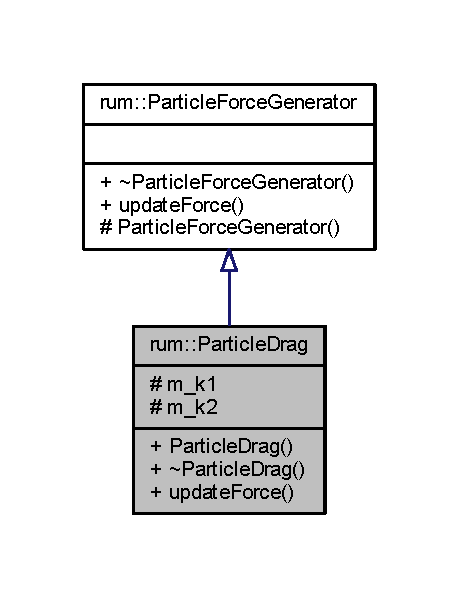
\includegraphics[width=220pt]{classrum_1_1_particle_drag__inherit__graph}
\end{center}
\end{figure}


Collaboration diagram for rum\+:\+:Particle\+Drag\+:\nopagebreak
\begin{figure}[H]
\begin{center}
\leavevmode
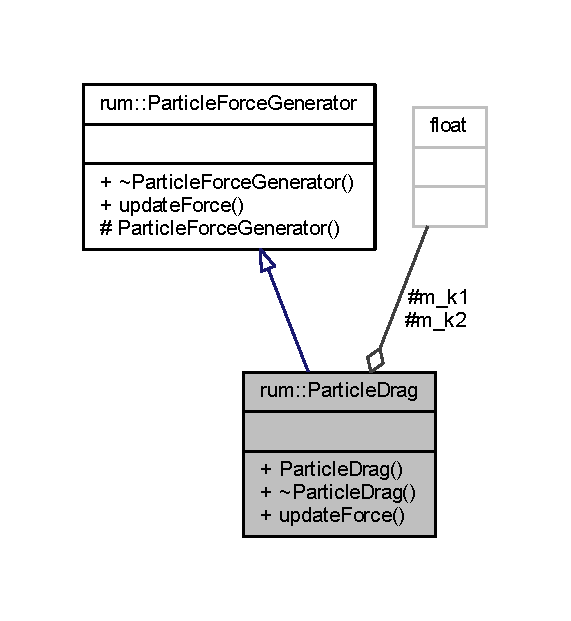
\includegraphics[width=274pt]{classrum_1_1_particle_drag__coll__graph}
\end{center}
\end{figure}
\subsection*{Public Member Functions}
\begin{DoxyCompactItemize}
\item 
\mbox{\hyperlink{classrum_1_1_particle_drag_a8489f5c5deb622003656afc4989e71bb}{Particle\+Drag}} (\mbox{\hyperlink{namespacerum_a7e8cca23573d5eaead0f138cbaa4862c}{real}} k1, \mbox{\hyperlink{namespacerum_a7e8cca23573d5eaead0f138cbaa4862c}{real}} k2)
\item 
\mbox{\hyperlink{classrum_1_1_particle_drag_a21072ca38b82529540f361a24cbec508}{$\sim$\+Particle\+Drag}} ()
\item 
void \mbox{\hyperlink{classrum_1_1_particle_drag_a61c989e4a66ae25372c5983178067525}{update\+Force}} (\mbox{\hyperlink{classrum_1_1_particle}{Particle}} $\ast$particle, \mbox{\hyperlink{namespacerum_a7e8cca23573d5eaead0f138cbaa4862c}{real}} duration) override
\end{DoxyCompactItemize}
\subsection*{Protected Attributes}
\begin{DoxyCompactItemize}
\item 
\mbox{\hyperlink{namespacerum_a7e8cca23573d5eaead0f138cbaa4862c}{real}} \mbox{\hyperlink{classrum_1_1_particle_drag_ad4fcf721667ea70b2ee8ca5ddac9d0ed}{m\+\_\+k1}}
\item 
\mbox{\hyperlink{namespacerum_a7e8cca23573d5eaead0f138cbaa4862c}{real}} \mbox{\hyperlink{classrum_1_1_particle_drag_a30f863703e55b68316c64c6f9a8cc25f}{m\+\_\+k2}}
\end{DoxyCompactItemize}
\subsection*{Additional Inherited Members}


\subsection{Constructor \& Destructor Documentation}
\mbox{\Hypertarget{classrum_1_1_particle_drag_a8489f5c5deb622003656afc4989e71bb}\label{classrum_1_1_particle_drag_a8489f5c5deb622003656afc4989e71bb}} 
\index{rum\+::\+Particle\+Drag@{rum\+::\+Particle\+Drag}!Particle\+Drag@{Particle\+Drag}}
\index{Particle\+Drag@{Particle\+Drag}!rum\+::\+Particle\+Drag@{rum\+::\+Particle\+Drag}}
\subsubsection{\texorpdfstring{Particle\+Drag()}{ParticleDrag()}}
{\footnotesize\ttfamily rum\+::\+Particle\+Drag\+::\+Particle\+Drag (\begin{DoxyParamCaption}\item[{\mbox{\hyperlink{namespacerum_a7e8cca23573d5eaead0f138cbaa4862c}{real}}}]{k1,  }\item[{\mbox{\hyperlink{namespacerum_a7e8cca23573d5eaead0f138cbaa4862c}{real}}}]{k2 }\end{DoxyParamCaption})}

\mbox{\Hypertarget{classrum_1_1_particle_drag_a21072ca38b82529540f361a24cbec508}\label{classrum_1_1_particle_drag_a21072ca38b82529540f361a24cbec508}} 
\index{rum\+::\+Particle\+Drag@{rum\+::\+Particle\+Drag}!````~Particle\+Drag@{$\sim$\+Particle\+Drag}}
\index{````~Particle\+Drag@{$\sim$\+Particle\+Drag}!rum\+::\+Particle\+Drag@{rum\+::\+Particle\+Drag}}
\subsubsection{\texorpdfstring{$\sim$\+Particle\+Drag()}{~ParticleDrag()}}
{\footnotesize\ttfamily rum\+::\+Particle\+Drag\+::$\sim$\+Particle\+Drag (\begin{DoxyParamCaption}{ }\end{DoxyParamCaption})}



\subsection{Member Function Documentation}
\mbox{\Hypertarget{classrum_1_1_particle_drag_a61c989e4a66ae25372c5983178067525}\label{classrum_1_1_particle_drag_a61c989e4a66ae25372c5983178067525}} 
\index{rum\+::\+Particle\+Drag@{rum\+::\+Particle\+Drag}!update\+Force@{update\+Force}}
\index{update\+Force@{update\+Force}!rum\+::\+Particle\+Drag@{rum\+::\+Particle\+Drag}}
\subsubsection{\texorpdfstring{update\+Force()}{updateForce()}}
{\footnotesize\ttfamily void rum\+::\+Particle\+Drag\+::update\+Force (\begin{DoxyParamCaption}\item[{\mbox{\hyperlink{classrum_1_1_particle}{Particle}} $\ast$}]{particle,  }\item[{\mbox{\hyperlink{namespacerum_a7e8cca23573d5eaead0f138cbaa4862c}{real}}}]{duration }\end{DoxyParamCaption})\hspace{0.3cm}{\ttfamily [override]}, {\ttfamily [virtual]}}



Implements \mbox{\hyperlink{classrum_1_1_particle_force_generator_af7abcafb9527220988ec4b9dde817b34}{rum\+::\+Particle\+Force\+Generator}}.



\subsection{Member Data Documentation}
\mbox{\Hypertarget{classrum_1_1_particle_drag_ad4fcf721667ea70b2ee8ca5ddac9d0ed}\label{classrum_1_1_particle_drag_ad4fcf721667ea70b2ee8ca5ddac9d0ed}} 
\index{rum\+::\+Particle\+Drag@{rum\+::\+Particle\+Drag}!m\+\_\+k1@{m\+\_\+k1}}
\index{m\+\_\+k1@{m\+\_\+k1}!rum\+::\+Particle\+Drag@{rum\+::\+Particle\+Drag}}
\subsubsection{\texorpdfstring{m\+\_\+k1}{m\_k1}}
{\footnotesize\ttfamily \mbox{\hyperlink{namespacerum_a7e8cca23573d5eaead0f138cbaa4862c}{real}} rum\+::\+Particle\+Drag\+::m\+\_\+k1\hspace{0.3cm}{\ttfamily [protected]}}

\mbox{\Hypertarget{classrum_1_1_particle_drag_a30f863703e55b68316c64c6f9a8cc25f}\label{classrum_1_1_particle_drag_a30f863703e55b68316c64c6f9a8cc25f}} 
\index{rum\+::\+Particle\+Drag@{rum\+::\+Particle\+Drag}!m\+\_\+k2@{m\+\_\+k2}}
\index{m\+\_\+k2@{m\+\_\+k2}!rum\+::\+Particle\+Drag@{rum\+::\+Particle\+Drag}}
\subsubsection{\texorpdfstring{m\+\_\+k2}{m\_k2}}
{\footnotesize\ttfamily \mbox{\hyperlink{namespacerum_a7e8cca23573d5eaead0f138cbaa4862c}{real}} rum\+::\+Particle\+Drag\+::m\+\_\+k2\hspace{0.3cm}{\ttfamily [protected]}}



The documentation for this class was generated from the following files\+:\begin{DoxyCompactItemize}
\item 
D\+:/\+Library/\+Documents/\+Job/\+Forschungsmaster/\+Projekte/\+Rumble3\+D/\+Rumble3\+D/include/\+R3\+D/\+Particle\+Engine/\mbox{\hyperlink{_particle_drag_8h}{Particle\+Drag.\+h}}\item 
D\+:/\+Library/\+Documents/\+Job/\+Forschungsmaster/\+Projekte/\+Rumble3\+D/\+Rumble3\+D/src/\+Particle\+Engine/\mbox{\hyperlink{_particle_drag_8cpp}{Particle\+Drag.\+cpp}}\end{DoxyCompactItemize}

\hypertarget{classrum_1_1_particle_force_generator}{}\section{rum\+:\+:Particle\+Force\+Generator Class Reference}
\label{classrum_1_1_particle_force_generator}\index{rum\+::\+Particle\+Force\+Generator@{rum\+::\+Particle\+Force\+Generator}}


{\ttfamily \#include $<$Particle\+Force\+Generator.\+h$>$}



Inheritance diagram for rum\+:\+:Particle\+Force\+Generator\+:\nopagebreak
\begin{figure}[H]
\begin{center}
\leavevmode
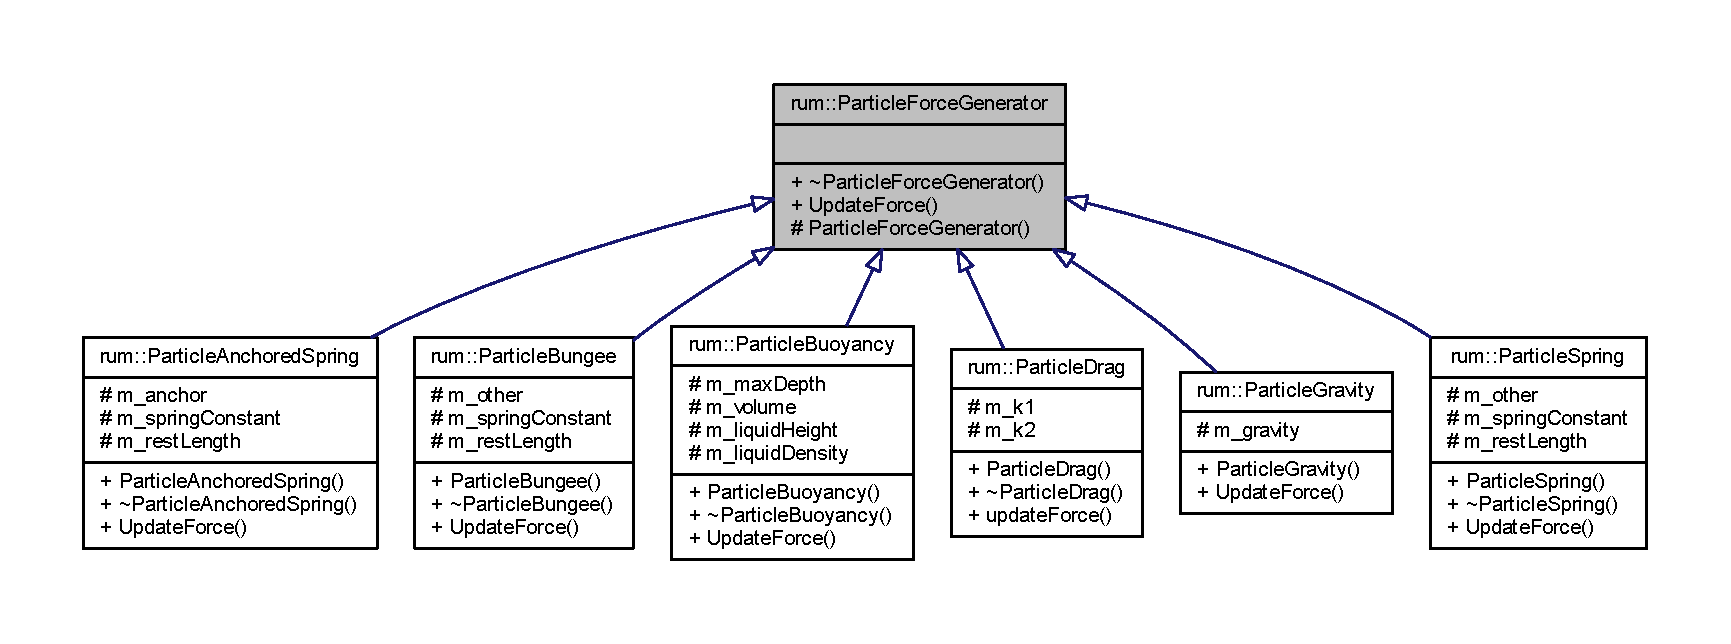
\includegraphics[width=350pt]{classrum_1_1_particle_force_generator__inherit__graph}
\end{center}
\end{figure}


Collaboration diagram for rum\+:\+:Particle\+Force\+Generator\+:\nopagebreak
\begin{figure}[H]
\begin{center}
\leavevmode
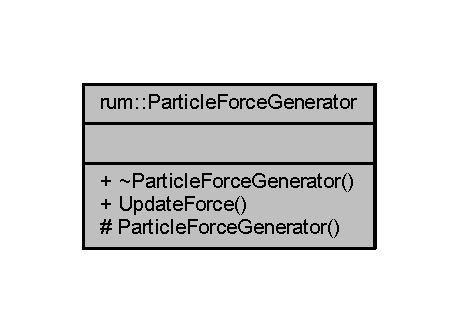
\includegraphics[width=220pt]{classrum_1_1_particle_force_generator__coll__graph}
\end{center}
\end{figure}
\subsection*{Public Member Functions}
\begin{DoxyCompactItemize}
\item 
virtual \hyperlink{classrum_1_1_particle_force_generator_aa6dd4ed9f382793958a76187e84fa104}{$\sim$\+Particle\+Force\+Generator} ()
\item 
virtual void \hyperlink{classrum_1_1_particle_force_generator_aca758295718deb8569796185ccbe8d54}{Update\+Force} (\hyperlink{classrum_1_1_particle}{Particle} $\ast$particle, \hyperlink{namespacerum_a7e8cca23573d5eaead0f138cbaa4862c}{real} duration)=0
\end{DoxyCompactItemize}
\subsection*{Protected Member Functions}
\begin{DoxyCompactItemize}
\item 
\hyperlink{classrum_1_1_particle_force_generator_a06c2ba0d0ed6d18353bb09f5e3c01ebf}{Particle\+Force\+Generator} ()
\end{DoxyCompactItemize}


\subsection{Constructor \& Destructor Documentation}
\mbox{\Hypertarget{classrum_1_1_particle_force_generator_aa6dd4ed9f382793958a76187e84fa104}\label{classrum_1_1_particle_force_generator_aa6dd4ed9f382793958a76187e84fa104}} 
\index{rum\+::\+Particle\+Force\+Generator@{rum\+::\+Particle\+Force\+Generator}!````~Particle\+Force\+Generator@{$\sim$\+Particle\+Force\+Generator}}
\index{````~Particle\+Force\+Generator@{$\sim$\+Particle\+Force\+Generator}!rum\+::\+Particle\+Force\+Generator@{rum\+::\+Particle\+Force\+Generator}}
\subsubsection{\texorpdfstring{$\sim$\+Particle\+Force\+Generator()}{~ParticleForceGenerator()}}
{\footnotesize\ttfamily rum\+::\+Particle\+Force\+Generator\+::$\sim$\+Particle\+Force\+Generator (\begin{DoxyParamCaption}{ }\end{DoxyParamCaption})\hspace{0.3cm}{\ttfamily [virtual]}}

\mbox{\Hypertarget{classrum_1_1_particle_force_generator_a06c2ba0d0ed6d18353bb09f5e3c01ebf}\label{classrum_1_1_particle_force_generator_a06c2ba0d0ed6d18353bb09f5e3c01ebf}} 
\index{rum\+::\+Particle\+Force\+Generator@{rum\+::\+Particle\+Force\+Generator}!Particle\+Force\+Generator@{Particle\+Force\+Generator}}
\index{Particle\+Force\+Generator@{Particle\+Force\+Generator}!rum\+::\+Particle\+Force\+Generator@{rum\+::\+Particle\+Force\+Generator}}
\subsubsection{\texorpdfstring{Particle\+Force\+Generator()}{ParticleForceGenerator()}}
{\footnotesize\ttfamily rum\+::\+Particle\+Force\+Generator\+::\+Particle\+Force\+Generator (\begin{DoxyParamCaption}{ }\end{DoxyParamCaption})\hspace{0.3cm}{\ttfamily [explicit]}, {\ttfamily [protected]}}



\subsection{Member Function Documentation}
\mbox{\Hypertarget{classrum_1_1_particle_force_generator_aca758295718deb8569796185ccbe8d54}\label{classrum_1_1_particle_force_generator_aca758295718deb8569796185ccbe8d54}} 
\index{rum\+::\+Particle\+Force\+Generator@{rum\+::\+Particle\+Force\+Generator}!Update\+Force@{Update\+Force}}
\index{Update\+Force@{Update\+Force}!rum\+::\+Particle\+Force\+Generator@{rum\+::\+Particle\+Force\+Generator}}
\subsubsection{\texorpdfstring{Update\+Force()}{UpdateForce()}}
{\footnotesize\ttfamily virtual void rum\+::\+Particle\+Force\+Generator\+::\+Update\+Force (\begin{DoxyParamCaption}\item[{\hyperlink{classrum_1_1_particle}{Particle} $\ast$}]{particle,  }\item[{\hyperlink{namespacerum_a7e8cca23573d5eaead0f138cbaa4862c}{real}}]{duration }\end{DoxyParamCaption})\hspace{0.3cm}{\ttfamily [pure virtual]}}



Implemented in \hyperlink{classrum_1_1_particle_anchored_spring_aa4fcab6f3de51c6b89f3a65b80814cc6}{rum\+::\+Particle\+Anchored\+Spring}, \hyperlink{classrum_1_1_particle_gravity_a8b943480e3856d1818e5090097403679}{rum\+::\+Particle\+Gravity}, \hyperlink{classrum_1_1_particle_bungee_a631e7f4c92c881b9a62471e2f75e2a2c}{rum\+::\+Particle\+Bungee}, \hyperlink{classrum_1_1_particle_buoyancy_aeda5d90f9ac512fdf63079739b9af0b7}{rum\+::\+Particle\+Buoyancy}, and \hyperlink{classrum_1_1_particle_spring_aed78e527b0a96a392fe5d9e1ffa50ca6}{rum\+::\+Particle\+Spring}.



The documentation for this class was generated from the following files\+:\begin{DoxyCompactItemize}
\item 
F\+:/\+Library/\+Documents/\+Job/\+Forschungsmaster/\+Rumble3\+D/\+Rumble3\+D/include/\+R3\+D/\+Particle\+Engine/\hyperlink{_particle_force_generator_8h}{Particle\+Force\+Generator.\+h}\item 
F\+:/\+Library/\+Documents/\+Job/\+Forschungsmaster/\+Rumble3\+D/\+Rumble3\+D/src/\+Particle\+Engine/\hyperlink{_particle_force_generator_8cpp}{Particle\+Force\+Generator.\+cpp}\end{DoxyCompactItemize}

\hypertarget{structrum_1_1_particle_force_registry_1_1_particle_force_registration_entry}{}\section{rum\+:\+:Particle\+Force\+Registry\+:\+:Particle\+Force\+Registration\+Entry Struct Reference}
\label{structrum_1_1_particle_force_registry_1_1_particle_force_registration_entry}\index{rum\+::\+Particle\+Force\+Registry\+::\+Particle\+Force\+Registration\+Entry@{rum\+::\+Particle\+Force\+Registry\+::\+Particle\+Force\+Registration\+Entry}}


{\ttfamily \#include $<$Particle\+Force\+Registry.\+h$>$}



Collaboration diagram for rum\+:\+:Particle\+Force\+Registry\+:\+:Particle\+Force\+Registration\+Entry\+:\nopagebreak
\begin{figure}[H]
\begin{center}
\leavevmode
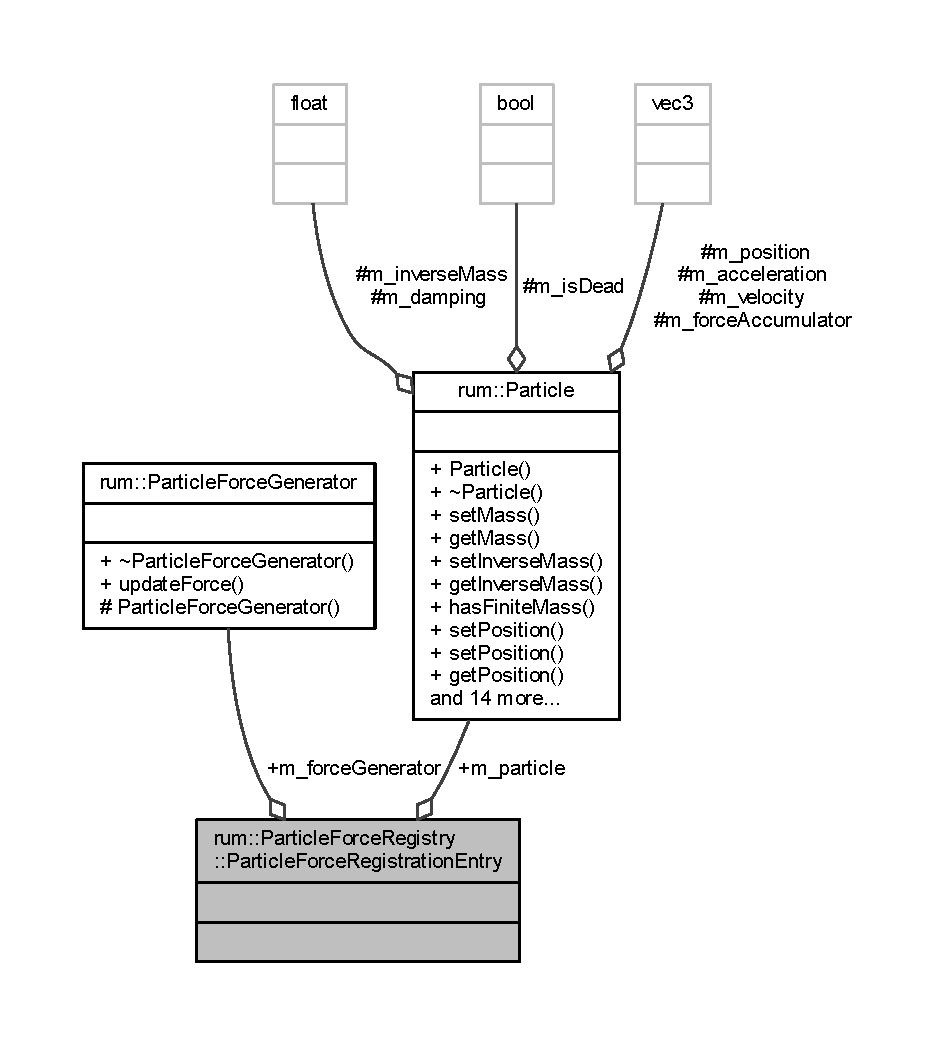
\includegraphics[width=350pt]{structrum_1_1_particle_force_registry_1_1_particle_force_registration_entry__coll__graph}
\end{center}
\end{figure}
\subsection*{Public Attributes}
\begin{DoxyCompactItemize}
\item 
\hyperlink{classrum_1_1_particle}{Particle} $\ast$ \hyperlink{structrum_1_1_particle_force_registry_1_1_particle_force_registration_entry_a9bf2865b17e61b75159bc197d0f84e3e}{particle}
\item 
\hyperlink{classrum_1_1_particle_force_generator}{Particle\+Force\+Generator} $\ast$ \hyperlink{structrum_1_1_particle_force_registry_1_1_particle_force_registration_entry_af067a2e67b30ccd345b584d1740334a7}{force\+Generator}
\end{DoxyCompactItemize}


\subsection{Member Data Documentation}
\mbox{\Hypertarget{structrum_1_1_particle_force_registry_1_1_particle_force_registration_entry_af067a2e67b30ccd345b584d1740334a7}\label{structrum_1_1_particle_force_registry_1_1_particle_force_registration_entry_af067a2e67b30ccd345b584d1740334a7}} 
\index{rum\+::\+Particle\+Force\+Registry\+::\+Particle\+Force\+Registration\+Entry@{rum\+::\+Particle\+Force\+Registry\+::\+Particle\+Force\+Registration\+Entry}!force\+Generator@{force\+Generator}}
\index{force\+Generator@{force\+Generator}!rum\+::\+Particle\+Force\+Registry\+::\+Particle\+Force\+Registration\+Entry@{rum\+::\+Particle\+Force\+Registry\+::\+Particle\+Force\+Registration\+Entry}}
\subsubsection{\texorpdfstring{force\+Generator}{forceGenerator}}
{\footnotesize\ttfamily \hyperlink{classrum_1_1_particle_force_generator}{Particle\+Force\+Generator}$\ast$ rum\+::\+Particle\+Force\+Registry\+::\+Particle\+Force\+Registration\+Entry\+::force\+Generator}

\mbox{\Hypertarget{structrum_1_1_particle_force_registry_1_1_particle_force_registration_entry_a9bf2865b17e61b75159bc197d0f84e3e}\label{structrum_1_1_particle_force_registry_1_1_particle_force_registration_entry_a9bf2865b17e61b75159bc197d0f84e3e}} 
\index{rum\+::\+Particle\+Force\+Registry\+::\+Particle\+Force\+Registration\+Entry@{rum\+::\+Particle\+Force\+Registry\+::\+Particle\+Force\+Registration\+Entry}!particle@{particle}}
\index{particle@{particle}!rum\+::\+Particle\+Force\+Registry\+::\+Particle\+Force\+Registration\+Entry@{rum\+::\+Particle\+Force\+Registry\+::\+Particle\+Force\+Registration\+Entry}}
\subsubsection{\texorpdfstring{particle}{particle}}
{\footnotesize\ttfamily \hyperlink{classrum_1_1_particle}{Particle}$\ast$ rum\+::\+Particle\+Force\+Registry\+::\+Particle\+Force\+Registration\+Entry\+::particle}



The documentation for this struct was generated from the following file\+:\begin{DoxyCompactItemize}
\item 
F\+:/\+Library/\+Documents/\+Job/\+Forschungsmaster/\+Rumble3\+D/\+Rumble3\+D/include/\+R3\+D/\+Particle\+Engine/\hyperlink{_particle_force_registry_8h}{Particle\+Force\+Registry.\+h}\end{DoxyCompactItemize}

\hypertarget{classrum_1_1_particle_force_registry}{}\section{rum\+:\+:Particle\+Force\+Registry Class Reference}
\label{classrum_1_1_particle_force_registry}\index{rum\+::\+Particle\+Force\+Registry@{rum\+::\+Particle\+Force\+Registry}}


{\ttfamily \#include $<$Particle\+Force\+Registry.\+h$>$}



Collaboration diagram for rum\+:\+:Particle\+Force\+Registry\+:\nopagebreak
\begin{figure}[H]
\begin{center}
\leavevmode
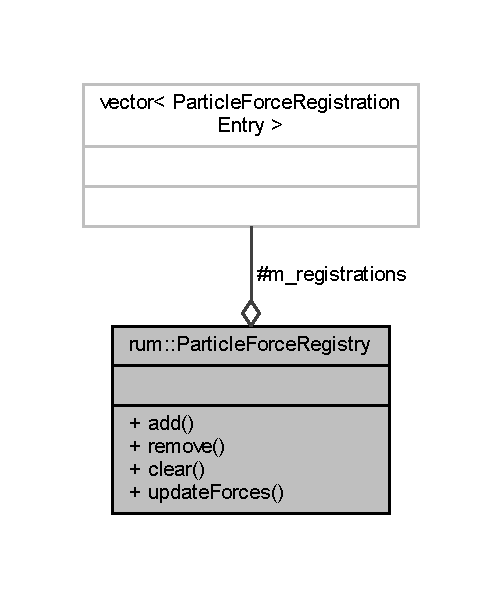
\includegraphics[width=241pt]{classrum_1_1_particle_force_registry__coll__graph}
\end{center}
\end{figure}
\subsection*{Classes}
\begin{DoxyCompactItemize}
\item 
struct \mbox{\hyperlink{structrum_1_1_particle_force_registry_1_1_particle_force_registration_entry}{Particle\+Force\+Registration\+Entry}}
\end{DoxyCompactItemize}
\subsection*{Public Member Functions}
\begin{DoxyCompactItemize}
\item 
void \mbox{\hyperlink{classrum_1_1_particle_force_registry_a9297d30559870d6a33a459430d2ac757}{add}} (\mbox{\hyperlink{classrum_1_1_particle}{Particle}} $\ast$particle, \mbox{\hyperlink{classrum_1_1_particle_force_generator}{Particle\+Force\+Generator}} $\ast$fg)
\item 
void \mbox{\hyperlink{classrum_1_1_particle_force_registry_a326fe2b591d058a3feea1effa5ac3a70}{remove}} (\mbox{\hyperlink{classrum_1_1_particle}{Particle}} $\ast$particle, \mbox{\hyperlink{classrum_1_1_particle_force_generator}{Particle\+Force\+Generator}} $\ast$fg)
\item 
void \mbox{\hyperlink{classrum_1_1_particle_force_registry_a856ccf8959632accfbec1abf67813b71}{clear}} ()
\item 
void \mbox{\hyperlink{classrum_1_1_particle_force_registry_a0c7ba8f4e4572243079e4e9758080aa0}{update\+Forces}} (\mbox{\hyperlink{namespacerum_a7e8cca23573d5eaead0f138cbaa4862c}{real}} duration)
\end{DoxyCompactItemize}
\subsection*{Protected Types}
\begin{DoxyCompactItemize}
\item 
typedef std\+::vector$<$ \mbox{\hyperlink{structrum_1_1_particle_force_registry_1_1_particle_force_registration_entry}{Particle\+Force\+Registration\+Entry}} $>$ \mbox{\hyperlink{classrum_1_1_particle_force_registry_a63b7b5a4c79dafe5b3658505c7ac1163}{Registry}}
\end{DoxyCompactItemize}
\subsection*{Protected Attributes}
\begin{DoxyCompactItemize}
\item 
\mbox{\hyperlink{classrum_1_1_particle_force_registry_a63b7b5a4c79dafe5b3658505c7ac1163}{Registry}} \mbox{\hyperlink{classrum_1_1_particle_force_registry_a650e1205958b828c0d501b812b35212a}{m\+\_\+registrations}}
\end{DoxyCompactItemize}


\subsection{Member Typedef Documentation}
\mbox{\Hypertarget{classrum_1_1_particle_force_registry_a63b7b5a4c79dafe5b3658505c7ac1163}\label{classrum_1_1_particle_force_registry_a63b7b5a4c79dafe5b3658505c7ac1163}} 
\index{rum\+::\+Particle\+Force\+Registry@{rum\+::\+Particle\+Force\+Registry}!Registry@{Registry}}
\index{Registry@{Registry}!rum\+::\+Particle\+Force\+Registry@{rum\+::\+Particle\+Force\+Registry}}
\subsubsection{\texorpdfstring{Registry}{Registry}}
{\footnotesize\ttfamily typedef std\+::vector$<$\mbox{\hyperlink{structrum_1_1_particle_force_registry_1_1_particle_force_registration_entry}{Particle\+Force\+Registration\+Entry}}$>$ \mbox{\hyperlink{classrum_1_1_particle_force_registry_a63b7b5a4c79dafe5b3658505c7ac1163}{rum\+::\+Particle\+Force\+Registry\+::\+Registry}}\hspace{0.3cm}{\ttfamily [protected]}}



\subsection{Member Function Documentation}
\mbox{\Hypertarget{classrum_1_1_particle_force_registry_a9297d30559870d6a33a459430d2ac757}\label{classrum_1_1_particle_force_registry_a9297d30559870d6a33a459430d2ac757}} 
\index{rum\+::\+Particle\+Force\+Registry@{rum\+::\+Particle\+Force\+Registry}!add@{add}}
\index{add@{add}!rum\+::\+Particle\+Force\+Registry@{rum\+::\+Particle\+Force\+Registry}}
\subsubsection{\texorpdfstring{add()}{add()}}
{\footnotesize\ttfamily void rum\+::\+Particle\+Force\+Registry\+::add (\begin{DoxyParamCaption}\item[{\mbox{\hyperlink{classrum_1_1_particle}{Particle}} $\ast$}]{particle,  }\item[{\mbox{\hyperlink{classrum_1_1_particle_force_generator}{Particle\+Force\+Generator}} $\ast$}]{fg }\end{DoxyParamCaption})}

\mbox{\Hypertarget{classrum_1_1_particle_force_registry_a856ccf8959632accfbec1abf67813b71}\label{classrum_1_1_particle_force_registry_a856ccf8959632accfbec1abf67813b71}} 
\index{rum\+::\+Particle\+Force\+Registry@{rum\+::\+Particle\+Force\+Registry}!clear@{clear}}
\index{clear@{clear}!rum\+::\+Particle\+Force\+Registry@{rum\+::\+Particle\+Force\+Registry}}
\subsubsection{\texorpdfstring{clear()}{clear()}}
{\footnotesize\ttfamily void rum\+::\+Particle\+Force\+Registry\+::clear (\begin{DoxyParamCaption}{ }\end{DoxyParamCaption})}

\mbox{\Hypertarget{classrum_1_1_particle_force_registry_a326fe2b591d058a3feea1effa5ac3a70}\label{classrum_1_1_particle_force_registry_a326fe2b591d058a3feea1effa5ac3a70}} 
\index{rum\+::\+Particle\+Force\+Registry@{rum\+::\+Particle\+Force\+Registry}!remove@{remove}}
\index{remove@{remove}!rum\+::\+Particle\+Force\+Registry@{rum\+::\+Particle\+Force\+Registry}}
\subsubsection{\texorpdfstring{remove()}{remove()}}
{\footnotesize\ttfamily void rum\+::\+Particle\+Force\+Registry\+::remove (\begin{DoxyParamCaption}\item[{\mbox{\hyperlink{classrum_1_1_particle}{Particle}} $\ast$}]{particle,  }\item[{\mbox{\hyperlink{classrum_1_1_particle_force_generator}{Particle\+Force\+Generator}} $\ast$}]{fg }\end{DoxyParamCaption})}

\mbox{\Hypertarget{classrum_1_1_particle_force_registry_a0c7ba8f4e4572243079e4e9758080aa0}\label{classrum_1_1_particle_force_registry_a0c7ba8f4e4572243079e4e9758080aa0}} 
\index{rum\+::\+Particle\+Force\+Registry@{rum\+::\+Particle\+Force\+Registry}!update\+Forces@{update\+Forces}}
\index{update\+Forces@{update\+Forces}!rum\+::\+Particle\+Force\+Registry@{rum\+::\+Particle\+Force\+Registry}}
\subsubsection{\texorpdfstring{update\+Forces()}{updateForces()}}
{\footnotesize\ttfamily void rum\+::\+Particle\+Force\+Registry\+::update\+Forces (\begin{DoxyParamCaption}\item[{\mbox{\hyperlink{namespacerum_a7e8cca23573d5eaead0f138cbaa4862c}{real}}}]{duration }\end{DoxyParamCaption})}



\subsection{Member Data Documentation}
\mbox{\Hypertarget{classrum_1_1_particle_force_registry_a650e1205958b828c0d501b812b35212a}\label{classrum_1_1_particle_force_registry_a650e1205958b828c0d501b812b35212a}} 
\index{rum\+::\+Particle\+Force\+Registry@{rum\+::\+Particle\+Force\+Registry}!m\+\_\+registrations@{m\+\_\+registrations}}
\index{m\+\_\+registrations@{m\+\_\+registrations}!rum\+::\+Particle\+Force\+Registry@{rum\+::\+Particle\+Force\+Registry}}
\subsubsection{\texorpdfstring{m\+\_\+registrations}{m\_registrations}}
{\footnotesize\ttfamily \mbox{\hyperlink{classrum_1_1_particle_force_registry_a63b7b5a4c79dafe5b3658505c7ac1163}{Registry}} rum\+::\+Particle\+Force\+Registry\+::m\+\_\+registrations\hspace{0.3cm}{\ttfamily [protected]}}



The documentation for this class was generated from the following files\+:\begin{DoxyCompactItemize}
\item 
D\+:/\+Library/\+Documents/\+Job/\+Forschungsmaster/\+Projekte/\+Rumble3\+D/\+Rumble3\+D/include/\+R3\+D/\+Particle\+Engine/\mbox{\hyperlink{_particle_force_registry_8h}{Particle\+Force\+Registry.\+h}}\item 
D\+:/\+Library/\+Documents/\+Job/\+Forschungsmaster/\+Projekte/\+Rumble3\+D/\+Rumble3\+D/src/\+Particle\+Engine/\mbox{\hyperlink{_particle_force_registry_8cpp}{Particle\+Force\+Registry.\+cpp}}\end{DoxyCompactItemize}

\hypertarget{classrum_1_1_particle_gravity}{}\section{rum\+:\+:Particle\+Gravity Class Reference}
\label{classrum_1_1_particle_gravity}\index{rum\+::\+Particle\+Gravity@{rum\+::\+Particle\+Gravity}}


{\ttfamily \#include $<$Particle\+Gravity.\+h$>$}



Inheritance diagram for rum\+:\+:Particle\+Gravity\+:\nopagebreak
\begin{figure}[H]
\begin{center}
\leavevmode
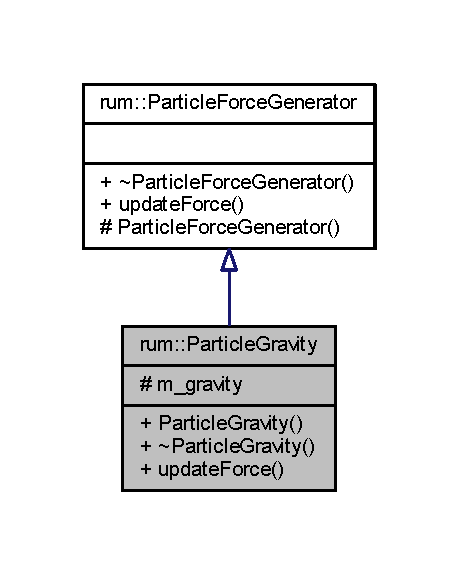
\includegraphics[width=220pt]{classrum_1_1_particle_gravity__inherit__graph}
\end{center}
\end{figure}


Collaboration diagram for rum\+:\+:Particle\+Gravity\+:\nopagebreak
\begin{figure}[H]
\begin{center}
\leavevmode
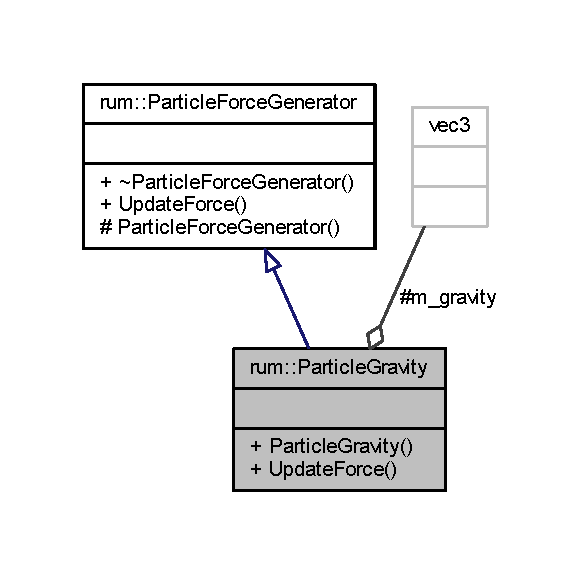
\includegraphics[width=281pt]{classrum_1_1_particle_gravity__coll__graph}
\end{center}
\end{figure}
\subsection*{Public Member Functions}
\begin{DoxyCompactItemize}
\item 
\mbox{\hyperlink{classrum_1_1_particle_gravity_af489016667073103233d0703ab2efbaa}{Particle\+Gravity}} (const glm\+::vec3 \&gravity)
\item 
\mbox{\hyperlink{classrum_1_1_particle_gravity_a4c09cee665172d402c6c545a3f9119ce}{$\sim$\+Particle\+Gravity}} ()
\item 
void \mbox{\hyperlink{classrum_1_1_particle_gravity_a52871a283cfef5377ef493bed81954a7}{update\+Force}} (\mbox{\hyperlink{classrum_1_1_particle}{Particle}} $\ast$particle, \mbox{\hyperlink{namespacerum_a7e8cca23573d5eaead0f138cbaa4862c}{real}} duration) override
\end{DoxyCompactItemize}
\subsection*{Protected Attributes}
\begin{DoxyCompactItemize}
\item 
glm\+::vec3 \mbox{\hyperlink{classrum_1_1_particle_gravity_a9fbc86ccd5d18e93626a6c4b0fc3b5e2}{m\+\_\+gravity}}
\end{DoxyCompactItemize}
\subsection*{Additional Inherited Members}


\subsection{Constructor \& Destructor Documentation}
\mbox{\Hypertarget{classrum_1_1_particle_gravity_af489016667073103233d0703ab2efbaa}\label{classrum_1_1_particle_gravity_af489016667073103233d0703ab2efbaa}} 
\index{rum\+::\+Particle\+Gravity@{rum\+::\+Particle\+Gravity}!Particle\+Gravity@{Particle\+Gravity}}
\index{Particle\+Gravity@{Particle\+Gravity}!rum\+::\+Particle\+Gravity@{rum\+::\+Particle\+Gravity}}
\subsubsection{\texorpdfstring{Particle\+Gravity()}{ParticleGravity()}}
{\footnotesize\ttfamily rum\+::\+Particle\+Gravity\+::\+Particle\+Gravity (\begin{DoxyParamCaption}\item[{const glm\+::vec3 \&}]{gravity }\end{DoxyParamCaption})\hspace{0.3cm}{\ttfamily [explicit]}}

\mbox{\Hypertarget{classrum_1_1_particle_gravity_a4c09cee665172d402c6c545a3f9119ce}\label{classrum_1_1_particle_gravity_a4c09cee665172d402c6c545a3f9119ce}} 
\index{rum\+::\+Particle\+Gravity@{rum\+::\+Particle\+Gravity}!````~Particle\+Gravity@{$\sim$\+Particle\+Gravity}}
\index{````~Particle\+Gravity@{$\sim$\+Particle\+Gravity}!rum\+::\+Particle\+Gravity@{rum\+::\+Particle\+Gravity}}
\subsubsection{\texorpdfstring{$\sim$\+Particle\+Gravity()}{~ParticleGravity()}}
{\footnotesize\ttfamily rum\+::\+Particle\+Gravity\+::$\sim$\+Particle\+Gravity (\begin{DoxyParamCaption}{ }\end{DoxyParamCaption})\hspace{0.3cm}{\ttfamily [default]}}



\subsection{Member Function Documentation}
\mbox{\Hypertarget{classrum_1_1_particle_gravity_a52871a283cfef5377ef493bed81954a7}\label{classrum_1_1_particle_gravity_a52871a283cfef5377ef493bed81954a7}} 
\index{rum\+::\+Particle\+Gravity@{rum\+::\+Particle\+Gravity}!update\+Force@{update\+Force}}
\index{update\+Force@{update\+Force}!rum\+::\+Particle\+Gravity@{rum\+::\+Particle\+Gravity}}
\subsubsection{\texorpdfstring{update\+Force()}{updateForce()}}
{\footnotesize\ttfamily void rum\+::\+Particle\+Gravity\+::update\+Force (\begin{DoxyParamCaption}\item[{\mbox{\hyperlink{classrum_1_1_particle}{Particle}} $\ast$}]{particle,  }\item[{\mbox{\hyperlink{namespacerum_a7e8cca23573d5eaead0f138cbaa4862c}{real}}}]{duration }\end{DoxyParamCaption})\hspace{0.3cm}{\ttfamily [override]}, {\ttfamily [virtual]}}



Implements \mbox{\hyperlink{classrum_1_1_particle_force_generator_af7abcafb9527220988ec4b9dde817b34}{rum\+::\+Particle\+Force\+Generator}}.



\subsection{Member Data Documentation}
\mbox{\Hypertarget{classrum_1_1_particle_gravity_a9fbc86ccd5d18e93626a6c4b0fc3b5e2}\label{classrum_1_1_particle_gravity_a9fbc86ccd5d18e93626a6c4b0fc3b5e2}} 
\index{rum\+::\+Particle\+Gravity@{rum\+::\+Particle\+Gravity}!m\+\_\+gravity@{m\+\_\+gravity}}
\index{m\+\_\+gravity@{m\+\_\+gravity}!rum\+::\+Particle\+Gravity@{rum\+::\+Particle\+Gravity}}
\subsubsection{\texorpdfstring{m\+\_\+gravity}{m\_gravity}}
{\footnotesize\ttfamily glm\+::vec3 rum\+::\+Particle\+Gravity\+::m\+\_\+gravity\hspace{0.3cm}{\ttfamily [protected]}}



The documentation for this class was generated from the following files\+:\begin{DoxyCompactItemize}
\item 
D\+:/\+Library/\+Documents/\+Job/\+Forschungsmaster/\+Projekte/\+Rumble3\+D/\+Rumble3\+D/include/\+R3\+D/\+Particle\+Engine/\mbox{\hyperlink{_particle_gravity_8h}{Particle\+Gravity.\+h}}\item 
D\+:/\+Library/\+Documents/\+Job/\+Forschungsmaster/\+Projekte/\+Rumble3\+D/\+Rumble3\+D/src/\+Particle\+Engine/\mbox{\hyperlink{_particle_gravity_8cpp}{Particle\+Gravity.\+cpp}}\end{DoxyCompactItemize}

\hypertarget{classrum_1_1_particle_link}{}\section{rum\+:\+:Particle\+Link Class Reference}
\label{classrum_1_1_particle_link}\index{rum\+::\+Particle\+Link@{rum\+::\+Particle\+Link}}


{\ttfamily \#include $<$Particle\+Link.\+h$>$}



Inheritance diagram for rum\+:\+:Particle\+Link\+:\nopagebreak
\begin{figure}[H]
\begin{center}
\leavevmode
\includegraphics[width=350pt]{classrum_1_1_particle_link__inherit__graph}
\end{center}
\end{figure}


Collaboration diagram for rum\+:\+:Particle\+Link\+:\nopagebreak
\begin{figure}[H]
\begin{center}
\leavevmode
\includegraphics[width=350pt]{classrum_1_1_particle_link__coll__graph}
\end{center}
\end{figure}
\subsection*{Public Member Functions}
\begin{DoxyCompactItemize}
\item 
virtual \mbox{\hyperlink{classrum_1_1_particle_link_a93add8689cecd885bfe9652d3d9dc440}{$\sim$\+Particle\+Link}} ()
\item 
unsigned int \mbox{\hyperlink{classrum_1_1_particle_link_a0da76619bd1d2ae04d5f8173c2883ff2}{add\+Contact}} (\mbox{\hyperlink{classrum_1_1_particle_contact}{Particle\+Contact}} $\ast$contact, unsigned int limit) const override=0
\item 
void \mbox{\hyperlink{classrum_1_1_particle_link_a9c9c83b1752a6b7e8d95658218402128}{set\+Particles}} (\mbox{\hyperlink{classrum_1_1_particle}{Particle}} $\ast$particle0, \mbox{\hyperlink{classrum_1_1_particle}{Particle}} $\ast$particle1=nullptr)
\end{DoxyCompactItemize}
\subsection*{Protected Member Functions}
\begin{DoxyCompactItemize}
\item 
\mbox{\hyperlink{classrum_1_1_particle_link_abcd2cccf1292b259443298ba7fc724d1}{Particle\+Link}} ()
\item 
\mbox{\hyperlink{namespacerum_a7e8cca23573d5eaead0f138cbaa4862c}{real}} \mbox{\hyperlink{classrum_1_1_particle_link_ad77a03be98566b0913aad0882e2283ac}{current\+Length}} () const
\end{DoxyCompactItemize}
\subsection*{Protected Attributes}
\begin{DoxyCompactItemize}
\item 
\mbox{\hyperlink{classrum_1_1_particle}{Particle}} $\ast$ \mbox{\hyperlink{classrum_1_1_particle_link_a0a919ccae0b5813620d5010d49094dc7}{m\+\_\+particles}} \mbox{[}2\mbox{]} \{\}
\end{DoxyCompactItemize}


\subsection{Constructor \& Destructor Documentation}
\mbox{\Hypertarget{classrum_1_1_particle_link_a93add8689cecd885bfe9652d3d9dc440}\label{classrum_1_1_particle_link_a93add8689cecd885bfe9652d3d9dc440}} 
\index{rum\+::\+Particle\+Link@{rum\+::\+Particle\+Link}!````~Particle\+Link@{$\sim$\+Particle\+Link}}
\index{````~Particle\+Link@{$\sim$\+Particle\+Link}!rum\+::\+Particle\+Link@{rum\+::\+Particle\+Link}}
\subsubsection{\texorpdfstring{$\sim$\+Particle\+Link()}{~ParticleLink()}}
{\footnotesize\ttfamily rum\+::\+Particle\+Link\+::$\sim$\+Particle\+Link (\begin{DoxyParamCaption}{ }\end{DoxyParamCaption})\hspace{0.3cm}{\ttfamily [virtual]}, {\ttfamily [default]}}

\mbox{\Hypertarget{classrum_1_1_particle_link_abcd2cccf1292b259443298ba7fc724d1}\label{classrum_1_1_particle_link_abcd2cccf1292b259443298ba7fc724d1}} 
\index{rum\+::\+Particle\+Link@{rum\+::\+Particle\+Link}!Particle\+Link@{Particle\+Link}}
\index{Particle\+Link@{Particle\+Link}!rum\+::\+Particle\+Link@{rum\+::\+Particle\+Link}}
\subsubsection{\texorpdfstring{Particle\+Link()}{ParticleLink()}}
{\footnotesize\ttfamily rum\+::\+Particle\+Link\+::\+Particle\+Link (\begin{DoxyParamCaption}{ }\end{DoxyParamCaption})\hspace{0.3cm}{\ttfamily [explicit]}, {\ttfamily [protected]}, {\ttfamily [default]}}



\subsection{Member Function Documentation}
\mbox{\Hypertarget{classrum_1_1_particle_link_a0da76619bd1d2ae04d5f8173c2883ff2}\label{classrum_1_1_particle_link_a0da76619bd1d2ae04d5f8173c2883ff2}} 
\index{rum\+::\+Particle\+Link@{rum\+::\+Particle\+Link}!add\+Contact@{add\+Contact}}
\index{add\+Contact@{add\+Contact}!rum\+::\+Particle\+Link@{rum\+::\+Particle\+Link}}
\subsubsection{\texorpdfstring{add\+Contact()}{addContact()}}
{\footnotesize\ttfamily unsigned int rum\+::\+Particle\+Link\+::add\+Contact (\begin{DoxyParamCaption}\item[{\mbox{\hyperlink{classrum_1_1_particle_contact}{Particle\+Contact}} $\ast$}]{contact,  }\item[{unsigned int}]{limit }\end{DoxyParamCaption}) const\hspace{0.3cm}{\ttfamily [override]}, {\ttfamily [pure virtual]}}



Implements \mbox{\hyperlink{classrum_1_1_particle_contact_generator_a343d3df815d7e170458fe937fe82aad5}{rum\+::\+Particle\+Contact\+Generator}}.



Implemented in \mbox{\hyperlink{classrum_1_1_particle_cable_a078344be0db7ccc00d326ac767736431}{rum\+::\+Particle\+Cable}}.

\mbox{\Hypertarget{classrum_1_1_particle_link_ad77a03be98566b0913aad0882e2283ac}\label{classrum_1_1_particle_link_ad77a03be98566b0913aad0882e2283ac}} 
\index{rum\+::\+Particle\+Link@{rum\+::\+Particle\+Link}!current\+Length@{current\+Length}}
\index{current\+Length@{current\+Length}!rum\+::\+Particle\+Link@{rum\+::\+Particle\+Link}}
\subsubsection{\texorpdfstring{current\+Length()}{currentLength()}}
{\footnotesize\ttfamily \mbox{\hyperlink{namespacerum_a7e8cca23573d5eaead0f138cbaa4862c}{real}} rum\+::\+Particle\+Link\+::current\+Length (\begin{DoxyParamCaption}{ }\end{DoxyParamCaption}) const\hspace{0.3cm}{\ttfamily [protected]}}

\mbox{\Hypertarget{classrum_1_1_particle_link_a9c9c83b1752a6b7e8d95658218402128}\label{classrum_1_1_particle_link_a9c9c83b1752a6b7e8d95658218402128}} 
\index{rum\+::\+Particle\+Link@{rum\+::\+Particle\+Link}!set\+Particles@{set\+Particles}}
\index{set\+Particles@{set\+Particles}!rum\+::\+Particle\+Link@{rum\+::\+Particle\+Link}}
\subsubsection{\texorpdfstring{set\+Particles()}{setParticles()}}
{\footnotesize\ttfamily void rum\+::\+Particle\+Link\+::set\+Particles (\begin{DoxyParamCaption}\item[{\mbox{\hyperlink{classrum_1_1_particle}{Particle}} $\ast$}]{particle0,  }\item[{\mbox{\hyperlink{classrum_1_1_particle}{Particle}} $\ast$}]{particle1 = {\ttfamily nullptr} }\end{DoxyParamCaption})}



\subsection{Member Data Documentation}
\mbox{\Hypertarget{classrum_1_1_particle_link_a0a919ccae0b5813620d5010d49094dc7}\label{classrum_1_1_particle_link_a0a919ccae0b5813620d5010d49094dc7}} 
\index{rum\+::\+Particle\+Link@{rum\+::\+Particle\+Link}!m\+\_\+particles@{m\+\_\+particles}}
\index{m\+\_\+particles@{m\+\_\+particles}!rum\+::\+Particle\+Link@{rum\+::\+Particle\+Link}}
\subsubsection{\texorpdfstring{m\+\_\+particles}{m\_particles}}
{\footnotesize\ttfamily \mbox{\hyperlink{classrum_1_1_particle}{Particle}}$\ast$ rum\+::\+Particle\+Link\+::m\+\_\+particles\mbox{[}2\mbox{]} \{\}\hspace{0.3cm}{\ttfamily [protected]}}



The documentation for this class was generated from the following files\+:\begin{DoxyCompactItemize}
\item 
D\+:/\+Library/\+Documents/\+Job/\+Forschungsmaster/\+Projekte/\+Rumble3\+D/\+Rumble3\+D/include/\+R3\+D/\+Particle\+Engine/\mbox{\hyperlink{_particle_link_8h}{Particle\+Link.\+h}}\item 
D\+:/\+Library/\+Documents/\+Job/\+Forschungsmaster/\+Projekte/\+Rumble3\+D/\+Rumble3\+D/src/\+Particle\+Engine/\mbox{\hyperlink{_particle_link_8cpp}{Particle\+Link.\+cpp}}\end{DoxyCompactItemize}

\hypertarget{classrum_1_1_particle_rod}{}\section{rum\+:\+:Particle\+Rod Class Reference}
\label{classrum_1_1_particle_rod}\index{rum\+::\+Particle\+Rod@{rum\+::\+Particle\+Rod}}


{\ttfamily \#include $<$Particle\+Rod.\+h$>$}



Inheritance diagram for rum\+:\+:Particle\+Rod\+:\nopagebreak
\begin{figure}[H]
\begin{center}
\leavevmode
\includegraphics[width=229pt]{classrum_1_1_particle_rod__inherit__graph}
\end{center}
\end{figure}


Collaboration diagram for rum\+:\+:Particle\+Rod\+:\nopagebreak
\begin{figure}[H]
\begin{center}
\leavevmode
\includegraphics[width=350pt]{classrum_1_1_particle_rod__coll__graph}
\end{center}
\end{figure}
\subsection*{Public Member Functions}
\begin{DoxyCompactItemize}
\item 
virtual \mbox{\hyperlink{classrum_1_1_particle_rod_a59886e0bd126236a5f4cf1098ac39122}{$\sim$\+Particle\+Rod}} ()
\end{DoxyCompactItemize}
\subsection*{Protected Member Functions}
\begin{DoxyCompactItemize}
\item 
\mbox{\hyperlink{classrum_1_1_particle_rod_a76dc622d8d214830fc8b270e7cc21efc}{Particle\+Rod}} ()
\end{DoxyCompactItemize}
\subsection*{Protected Attributes}
\begin{DoxyCompactItemize}
\item 
\mbox{\hyperlink{namespacerum_a7e8cca23573d5eaead0f138cbaa4862c}{real}} \mbox{\hyperlink{classrum_1_1_particle_rod_a9f5c266ef3a91afc3f3c41b7c0f300a9}{m\+\_\+length}} \{\}
\end{DoxyCompactItemize}


\subsection{Constructor \& Destructor Documentation}
\mbox{\Hypertarget{classrum_1_1_particle_rod_a59886e0bd126236a5f4cf1098ac39122}\label{classrum_1_1_particle_rod_a59886e0bd126236a5f4cf1098ac39122}} 
\index{rum\+::\+Particle\+Rod@{rum\+::\+Particle\+Rod}!````~Particle\+Rod@{$\sim$\+Particle\+Rod}}
\index{````~Particle\+Rod@{$\sim$\+Particle\+Rod}!rum\+::\+Particle\+Rod@{rum\+::\+Particle\+Rod}}
\subsubsection{\texorpdfstring{$\sim$\+Particle\+Rod()}{~ParticleRod()}}
{\footnotesize\ttfamily rum\+::\+Particle\+Rod\+::$\sim$\+Particle\+Rod (\begin{DoxyParamCaption}{ }\end{DoxyParamCaption})\hspace{0.3cm}{\ttfamily [virtual]}, {\ttfamily [default]}}

\mbox{\Hypertarget{classrum_1_1_particle_rod_a76dc622d8d214830fc8b270e7cc21efc}\label{classrum_1_1_particle_rod_a76dc622d8d214830fc8b270e7cc21efc}} 
\index{rum\+::\+Particle\+Rod@{rum\+::\+Particle\+Rod}!Particle\+Rod@{Particle\+Rod}}
\index{Particle\+Rod@{Particle\+Rod}!rum\+::\+Particle\+Rod@{rum\+::\+Particle\+Rod}}
\subsubsection{\texorpdfstring{Particle\+Rod()}{ParticleRod()}}
{\footnotesize\ttfamily rum\+::\+Particle\+Rod\+::\+Particle\+Rod (\begin{DoxyParamCaption}{ }\end{DoxyParamCaption})\hspace{0.3cm}{\ttfamily [explicit]}, {\ttfamily [protected]}, {\ttfamily [default]}}



\subsection{Member Data Documentation}
\mbox{\Hypertarget{classrum_1_1_particle_rod_a9f5c266ef3a91afc3f3c41b7c0f300a9}\label{classrum_1_1_particle_rod_a9f5c266ef3a91afc3f3c41b7c0f300a9}} 
\index{rum\+::\+Particle\+Rod@{rum\+::\+Particle\+Rod}!m\+\_\+length@{m\+\_\+length}}
\index{m\+\_\+length@{m\+\_\+length}!rum\+::\+Particle\+Rod@{rum\+::\+Particle\+Rod}}
\subsubsection{\texorpdfstring{m\+\_\+length}{m\_length}}
{\footnotesize\ttfamily \mbox{\hyperlink{namespacerum_a7e8cca23573d5eaead0f138cbaa4862c}{real}} rum\+::\+Particle\+Rod\+::m\+\_\+length \{\}\hspace{0.3cm}{\ttfamily [protected]}}



The documentation for this class was generated from the following files\+:\begin{DoxyCompactItemize}
\item 
D\+:/\+Library/\+Documents/\+Job/\+Forschungsmaster/\+Projekte/\+Rumble3\+D/\+Rumble3\+D/include/\+R3\+D/\+Particle\+Engine/\mbox{\hyperlink{_particle_rod_8h}{Particle\+Rod.\+h}}\item 
D\+:/\+Library/\+Documents/\+Job/\+Forschungsmaster/\+Projekte/\+Rumble3\+D/\+Rumble3\+D/src/\+Particle\+Engine/\mbox{\hyperlink{_particle_rod_8cpp}{Particle\+Rod.\+cpp}}\end{DoxyCompactItemize}

\hypertarget{classrum_1_1_particle_spring}{}\section{rum\+:\+:Particle\+Spring Class Reference}
\label{classrum_1_1_particle_spring}\index{rum\+::\+Particle\+Spring@{rum\+::\+Particle\+Spring}}


{\ttfamily \#include $<$Particle\+Spring.\+h$>$}



Inheritance diagram for rum\+:\+:Particle\+Spring\+:\nopagebreak
\begin{figure}[H]
\begin{center}
\leavevmode
\includegraphics[width=220pt]{classrum_1_1_particle_spring__inherit__graph}
\end{center}
\end{figure}


Collaboration diagram for rum\+:\+:Particle\+Spring\+:\nopagebreak
\begin{figure}[H]
\begin{center}
\leavevmode
\includegraphics[width=350pt]{classrum_1_1_particle_spring__coll__graph}
\end{center}
\end{figure}
\subsection*{Public Member Functions}
\begin{DoxyCompactItemize}
\item 
\hyperlink{classrum_1_1_particle_spring_af66a4191e6d0e567d0f88cc60f398c63}{Particle\+Spring} (\hyperlink{classrum_1_1_particle}{Particle} $\ast$other, \hyperlink{namespacerum_a7e8cca23573d5eaead0f138cbaa4862c}{real} spring\+Constant, \hyperlink{namespacerum_a7e8cca23573d5eaead0f138cbaa4862c}{real} rest\+Length)
\item 
\hyperlink{classrum_1_1_particle_spring_ac48ba65487b023ea754b4e0e8a33dafc}{$\sim$\+Particle\+Spring} ()
\item 
virtual void \hyperlink{classrum_1_1_particle_spring_aed78e527b0a96a392fe5d9e1ffa50ca6}{Update\+Force} (\hyperlink{classrum_1_1_particle}{Particle} $\ast$particle, \hyperlink{namespacerum_a7e8cca23573d5eaead0f138cbaa4862c}{real} duration)
\end{DoxyCompactItemize}
\subsection*{Protected Attributes}
\begin{DoxyCompactItemize}
\item 
\hyperlink{classrum_1_1_particle}{Particle} $\ast$ \hyperlink{classrum_1_1_particle_spring_aa09612b88d608ed80225c05baddfc0a3}{m\+\_\+other}
\item 
\hyperlink{namespacerum_a7e8cca23573d5eaead0f138cbaa4862c}{real} \hyperlink{classrum_1_1_particle_spring_ab799a061ff48edc65244d2df25a443ee}{m\+\_\+spring\+Constant}
\item 
\hyperlink{namespacerum_a7e8cca23573d5eaead0f138cbaa4862c}{real} \hyperlink{classrum_1_1_particle_spring_a4e126e603b40716ece3ef38108290dae}{m\+\_\+rest\+Length}
\end{DoxyCompactItemize}
\subsection*{Additional Inherited Members}


\subsection{Constructor \& Destructor Documentation}
\mbox{\Hypertarget{classrum_1_1_particle_spring_af66a4191e6d0e567d0f88cc60f398c63}\label{classrum_1_1_particle_spring_af66a4191e6d0e567d0f88cc60f398c63}} 
\index{rum\+::\+Particle\+Spring@{rum\+::\+Particle\+Spring}!Particle\+Spring@{Particle\+Spring}}
\index{Particle\+Spring@{Particle\+Spring}!rum\+::\+Particle\+Spring@{rum\+::\+Particle\+Spring}}
\subsubsection{\texorpdfstring{Particle\+Spring()}{ParticleSpring()}}
{\footnotesize\ttfamily rum\+::\+Particle\+Spring\+::\+Particle\+Spring (\begin{DoxyParamCaption}\item[{\hyperlink{classrum_1_1_particle}{Particle} $\ast$}]{other,  }\item[{\hyperlink{namespacerum_a7e8cca23573d5eaead0f138cbaa4862c}{real}}]{spring\+Constant,  }\item[{\hyperlink{namespacerum_a7e8cca23573d5eaead0f138cbaa4862c}{real}}]{rest\+Length }\end{DoxyParamCaption})}

\mbox{\Hypertarget{classrum_1_1_particle_spring_ac48ba65487b023ea754b4e0e8a33dafc}\label{classrum_1_1_particle_spring_ac48ba65487b023ea754b4e0e8a33dafc}} 
\index{rum\+::\+Particle\+Spring@{rum\+::\+Particle\+Spring}!````~Particle\+Spring@{$\sim$\+Particle\+Spring}}
\index{````~Particle\+Spring@{$\sim$\+Particle\+Spring}!rum\+::\+Particle\+Spring@{rum\+::\+Particle\+Spring}}
\subsubsection{\texorpdfstring{$\sim$\+Particle\+Spring()}{~ParticleSpring()}}
{\footnotesize\ttfamily rum\+::\+Particle\+Spring\+::$\sim$\+Particle\+Spring (\begin{DoxyParamCaption}{ }\end{DoxyParamCaption})}



\subsection{Member Function Documentation}
\mbox{\Hypertarget{classrum_1_1_particle_spring_aed78e527b0a96a392fe5d9e1ffa50ca6}\label{classrum_1_1_particle_spring_aed78e527b0a96a392fe5d9e1ffa50ca6}} 
\index{rum\+::\+Particle\+Spring@{rum\+::\+Particle\+Spring}!Update\+Force@{Update\+Force}}
\index{Update\+Force@{Update\+Force}!rum\+::\+Particle\+Spring@{rum\+::\+Particle\+Spring}}
\subsubsection{\texorpdfstring{Update\+Force()}{UpdateForce()}}
{\footnotesize\ttfamily void rum\+::\+Particle\+Spring\+::\+Update\+Force (\begin{DoxyParamCaption}\item[{\hyperlink{classrum_1_1_particle}{Particle} $\ast$}]{particle,  }\item[{\hyperlink{namespacerum_a7e8cca23573d5eaead0f138cbaa4862c}{real}}]{duration }\end{DoxyParamCaption})\hspace{0.3cm}{\ttfamily [virtual]}}



Implements \hyperlink{classrum_1_1_particle_force_generator_aca758295718deb8569796185ccbe8d54}{rum\+::\+Particle\+Force\+Generator}.



\subsection{Member Data Documentation}
\mbox{\Hypertarget{classrum_1_1_particle_spring_aa09612b88d608ed80225c05baddfc0a3}\label{classrum_1_1_particle_spring_aa09612b88d608ed80225c05baddfc0a3}} 
\index{rum\+::\+Particle\+Spring@{rum\+::\+Particle\+Spring}!m\+\_\+other@{m\+\_\+other}}
\index{m\+\_\+other@{m\+\_\+other}!rum\+::\+Particle\+Spring@{rum\+::\+Particle\+Spring}}
\subsubsection{\texorpdfstring{m\+\_\+other}{m\_other}}
{\footnotesize\ttfamily \hyperlink{classrum_1_1_particle}{Particle}$\ast$ rum\+::\+Particle\+Spring\+::m\+\_\+other\hspace{0.3cm}{\ttfamily [protected]}}

\mbox{\Hypertarget{classrum_1_1_particle_spring_a4e126e603b40716ece3ef38108290dae}\label{classrum_1_1_particle_spring_a4e126e603b40716ece3ef38108290dae}} 
\index{rum\+::\+Particle\+Spring@{rum\+::\+Particle\+Spring}!m\+\_\+rest\+Length@{m\+\_\+rest\+Length}}
\index{m\+\_\+rest\+Length@{m\+\_\+rest\+Length}!rum\+::\+Particle\+Spring@{rum\+::\+Particle\+Spring}}
\subsubsection{\texorpdfstring{m\+\_\+rest\+Length}{m\_restLength}}
{\footnotesize\ttfamily \hyperlink{namespacerum_a7e8cca23573d5eaead0f138cbaa4862c}{real} rum\+::\+Particle\+Spring\+::m\+\_\+rest\+Length\hspace{0.3cm}{\ttfamily [protected]}}

\mbox{\Hypertarget{classrum_1_1_particle_spring_ab799a061ff48edc65244d2df25a443ee}\label{classrum_1_1_particle_spring_ab799a061ff48edc65244d2df25a443ee}} 
\index{rum\+::\+Particle\+Spring@{rum\+::\+Particle\+Spring}!m\+\_\+spring\+Constant@{m\+\_\+spring\+Constant}}
\index{m\+\_\+spring\+Constant@{m\+\_\+spring\+Constant}!rum\+::\+Particle\+Spring@{rum\+::\+Particle\+Spring}}
\subsubsection{\texorpdfstring{m\+\_\+spring\+Constant}{m\_springConstant}}
{\footnotesize\ttfamily \hyperlink{namespacerum_a7e8cca23573d5eaead0f138cbaa4862c}{real} rum\+::\+Particle\+Spring\+::m\+\_\+spring\+Constant\hspace{0.3cm}{\ttfamily [protected]}}



The documentation for this class was generated from the following files\+:\begin{DoxyCompactItemize}
\item 
F\+:/\+Library/\+Documents/\+Job/\+Forschungsmaster/\+Rumble3\+D/\+Rumble3\+D/include/\+R3\+D/\+Particle\+Engine/\hyperlink{_particle_spring_8h}{Particle\+Spring.\+h}\item 
F\+:/\+Library/\+Documents/\+Job/\+Forschungsmaster/\+Rumble3\+D/\+Rumble3\+D/src/\+Particle\+Engine/\hyperlink{_particle_spring_8cpp}{Particle\+Spring.\+cpp}\end{DoxyCompactItemize}

\hypertarget{classrum_1_1_particle_world}{}\section{rum\+:\+:Particle\+World Class Reference}
\label{classrum_1_1_particle_world}\index{rum\+::\+Particle\+World@{rum\+::\+Particle\+World}}


{\ttfamily \#include $<$Particle\+World.\+h$>$}



Inheritance diagram for rum\+:\+:Particle\+World\+:\nopagebreak
\begin{figure}[H]
\begin{center}
\leavevmode
\includegraphics[width=239pt]{classrum_1_1_particle_world__inherit__graph}
\end{center}
\end{figure}


Collaboration diagram for rum\+:\+:Particle\+World\+:\nopagebreak
\begin{figure}[H]
\begin{center}
\leavevmode
\includegraphics[height=550pt]{classrum_1_1_particle_world__coll__graph}
\end{center}
\end{figure}
\subsection*{Public Types}
\begin{DoxyCompactItemize}
\item 
using \hyperlink{classrum_1_1_particle_world_ac172daef7c571097de59488881afa300}{Particles} = std\+::vector$<$ \hyperlink{classrum_1_1_particle}{Particle} $\ast$ $>$
\item 
using \hyperlink{classrum_1_1_particle_world_a78bc596aacdfcee5c3b788fb350a84c1}{Contact\+Generators} = std\+::vector$<$ \hyperlink{classrum_1_1_particle_contact_generator}{Particle\+Contact\+Generator} $\ast$ $>$
\end{DoxyCompactItemize}
\subsection*{Public Member Functions}
\begin{DoxyCompactItemize}
\item 
\hyperlink{classrum_1_1_particle_world_a1de60a26fde85310d906b829bd20e5d1}{Particle\+World} (unsigned int max\+Contacts, unsigned int iterations=0)
\item 
\hyperlink{classrum_1_1_particle_world_a8aaca4550e9469cd4a363fedee6ed75c}{$\sim$\+Particle\+World} ()
\item 
virtual void \hyperlink{classrum_1_1_particle_world_add8060f77975d47e984a0e0a3d1a0c0c}{On\+Begin} () override
\item 
virtual void \hyperlink{classrum_1_1_particle_world_ab30292cabe306715e49b5234abff1f3c}{Reset} () override
\item 
virtual void \hyperlink{classrum_1_1_particle_world_a3d71b71a6a76744b75990e1c53efd92e}{Step} (const \hyperlink{namespacerum_a7e8cca23573d5eaead0f138cbaa4862c}{real} time\+Delta) override
\item 
virtual void \hyperlink{classrum_1_1_particle_world_a8537914776ce477d40ff97ed7b7730d2}{Integrate} (\hyperlink{namespacerum_a7e8cca23573d5eaead0f138cbaa4862c}{real} duration) override
\item 
void \hyperlink{classrum_1_1_particle_world_a082a750fe9f9ebe0f2b9537fe62eeb71}{Add\+Particle} (\hyperlink{classrum_1_1_particle}{Particle} $\ast$p)
\item 
void \hyperlink{classrum_1_1_particle_world_a1e1ec7ffcd63ea5e1387de1fa1b8bea4}{Remove\+Particle} (\hyperlink{classrum_1_1_particle}{Particle} $\ast$p)
\item 
void \hyperlink{classrum_1_1_particle_world_a8b83f021e1fe1634e109c2854a1bd0e6}{Remove\+All\+Particles} ()
\item 
void \hyperlink{classrum_1_1_particle_world_a6ee40c3bfe3cae4667f68be881d43958}{Add\+Contact\+Generator} (\hyperlink{classrum_1_1_particle_contact_generator}{Particle\+Contact\+Generator} $\ast$pcg)
\item 
void \hyperlink{classrum_1_1_particle_world_abd7e00ca94ac98c4e410808227ca343a}{Remove\+Contact\+Generator} (\hyperlink{classrum_1_1_particle_contact_generator}{Particle\+Contact\+Generator} $\ast$pcg)
\item 
void \hyperlink{classrum_1_1_particle_world_a1cce582ad1d87d19246d821ac8d21a8b}{Remove\+All\+Contact\+Generators} ()
\item 
\hyperlink{classrum_1_1_particle_force_registry}{Particle\+Force\+Registry} \& \hyperlink{classrum_1_1_particle_world_a3a4d112218f537a590d2f482dea25d6c}{Get\+Particle\+Force\+Registry} ()
\end{DoxyCompactItemize}
\subsection*{Additional Inherited Members}


\subsection{Member Typedef Documentation}
\mbox{\Hypertarget{classrum_1_1_particle_world_a78bc596aacdfcee5c3b788fb350a84c1}\label{classrum_1_1_particle_world_a78bc596aacdfcee5c3b788fb350a84c1}} 
\index{rum\+::\+Particle\+World@{rum\+::\+Particle\+World}!Contact\+Generators@{Contact\+Generators}}
\index{Contact\+Generators@{Contact\+Generators}!rum\+::\+Particle\+World@{rum\+::\+Particle\+World}}
\subsubsection{\texorpdfstring{Contact\+Generators}{ContactGenerators}}
{\footnotesize\ttfamily using \hyperlink{classrum_1_1_particle_world_a78bc596aacdfcee5c3b788fb350a84c1}{rum\+::\+Particle\+World\+::\+Contact\+Generators} =  std\+::vector$<$\hyperlink{classrum_1_1_particle_contact_generator}{Particle\+Contact\+Generator}$\ast$$>$}

\mbox{\Hypertarget{classrum_1_1_particle_world_ac172daef7c571097de59488881afa300}\label{classrum_1_1_particle_world_ac172daef7c571097de59488881afa300}} 
\index{rum\+::\+Particle\+World@{rum\+::\+Particle\+World}!Particles@{Particles}}
\index{Particles@{Particles}!rum\+::\+Particle\+World@{rum\+::\+Particle\+World}}
\subsubsection{\texorpdfstring{Particles}{Particles}}
{\footnotesize\ttfamily using \hyperlink{classrum_1_1_particle_world_ac172daef7c571097de59488881afa300}{rum\+::\+Particle\+World\+::\+Particles} =  std\+::vector$<$\hyperlink{classrum_1_1_particle}{Particle}$\ast$$>$}



\subsection{Constructor \& Destructor Documentation}
\mbox{\Hypertarget{classrum_1_1_particle_world_a1de60a26fde85310d906b829bd20e5d1}\label{classrum_1_1_particle_world_a1de60a26fde85310d906b829bd20e5d1}} 
\index{rum\+::\+Particle\+World@{rum\+::\+Particle\+World}!Particle\+World@{Particle\+World}}
\index{Particle\+World@{Particle\+World}!rum\+::\+Particle\+World@{rum\+::\+Particle\+World}}
\subsubsection{\texorpdfstring{Particle\+World()}{ParticleWorld()}}
{\footnotesize\ttfamily rum\+::\+Particle\+World\+::\+Particle\+World (\begin{DoxyParamCaption}\item[{unsigned int}]{max\+Contacts,  }\item[{unsigned int}]{iterations = {\ttfamily 0} }\end{DoxyParamCaption})}

Teilchen-\/\+Simulator mit max\+Contacts Kontakten und einer optionalen Anzahl Iterationen. Falls iterations == 0, dann werden 2 $\ast$ Anzahl der Kontakte Iterationen durchgef�hrt. \mbox{\Hypertarget{classrum_1_1_particle_world_a8aaca4550e9469cd4a363fedee6ed75c}\label{classrum_1_1_particle_world_a8aaca4550e9469cd4a363fedee6ed75c}} 
\index{rum\+::\+Particle\+World@{rum\+::\+Particle\+World}!````~Particle\+World@{$\sim$\+Particle\+World}}
\index{````~Particle\+World@{$\sim$\+Particle\+World}!rum\+::\+Particle\+World@{rum\+::\+Particle\+World}}
\subsubsection{\texorpdfstring{$\sim$\+Particle\+World()}{~ParticleWorld()}}
{\footnotesize\ttfamily rum\+::\+Particle\+World\+::$\sim$\+Particle\+World (\begin{DoxyParamCaption}{ }\end{DoxyParamCaption})}



\subsection{Member Function Documentation}
\mbox{\Hypertarget{classrum_1_1_particle_world_a6ee40c3bfe3cae4667f68be881d43958}\label{classrum_1_1_particle_world_a6ee40c3bfe3cae4667f68be881d43958}} 
\index{rum\+::\+Particle\+World@{rum\+::\+Particle\+World}!Add\+Contact\+Generator@{Add\+Contact\+Generator}}
\index{Add\+Contact\+Generator@{Add\+Contact\+Generator}!rum\+::\+Particle\+World@{rum\+::\+Particle\+World}}
\subsubsection{\texorpdfstring{Add\+Contact\+Generator()}{AddContactGenerator()}}
{\footnotesize\ttfamily void rum\+::\+Particle\+World\+::\+Add\+Contact\+Generator (\begin{DoxyParamCaption}\item[{\hyperlink{classrum_1_1_particle_contact_generator}{Particle\+Contact\+Generator} $\ast$}]{pcg }\end{DoxyParamCaption})}

Add another contact generator \mbox{\Hypertarget{classrum_1_1_particle_world_a082a750fe9f9ebe0f2b9537fe62eeb71}\label{classrum_1_1_particle_world_a082a750fe9f9ebe0f2b9537fe62eeb71}} 
\index{rum\+::\+Particle\+World@{rum\+::\+Particle\+World}!Add\+Particle@{Add\+Particle}}
\index{Add\+Particle@{Add\+Particle}!rum\+::\+Particle\+World@{rum\+::\+Particle\+World}}
\subsubsection{\texorpdfstring{Add\+Particle()}{AddParticle()}}
{\footnotesize\ttfamily void rum\+::\+Particle\+World\+::\+Add\+Particle (\begin{DoxyParamCaption}\item[{\hyperlink{classrum_1_1_particle}{Particle} $\ast$}]{p }\end{DoxyParamCaption})}

Add another particle \mbox{\Hypertarget{classrum_1_1_particle_world_a3a4d112218f537a590d2f482dea25d6c}\label{classrum_1_1_particle_world_a3a4d112218f537a590d2f482dea25d6c}} 
\index{rum\+::\+Particle\+World@{rum\+::\+Particle\+World}!Get\+Particle\+Force\+Registry@{Get\+Particle\+Force\+Registry}}
\index{Get\+Particle\+Force\+Registry@{Get\+Particle\+Force\+Registry}!rum\+::\+Particle\+World@{rum\+::\+Particle\+World}}
\subsubsection{\texorpdfstring{Get\+Particle\+Force\+Registry()}{GetParticleForceRegistry()}}
{\footnotesize\ttfamily \hyperlink{classrum_1_1_particle_force_registry}{rum\+::\+Particle\+Force\+Registry} \& rum\+::\+Particle\+World\+::\+Get\+Particle\+Force\+Registry (\begin{DoxyParamCaption}{ }\end{DoxyParamCaption})}

Needed to bind particles to particle force generators \mbox{\Hypertarget{classrum_1_1_particle_world_a8537914776ce477d40ff97ed7b7730d2}\label{classrum_1_1_particle_world_a8537914776ce477d40ff97ed7b7730d2}} 
\index{rum\+::\+Particle\+World@{rum\+::\+Particle\+World}!Integrate@{Integrate}}
\index{Integrate@{Integrate}!rum\+::\+Particle\+World@{rum\+::\+Particle\+World}}
\subsubsection{\texorpdfstring{Integrate()}{Integrate()}}
{\footnotesize\ttfamily void rum\+::\+Particle\+World\+::\+Integrate (\begin{DoxyParamCaption}\item[{\hyperlink{namespacerum_a7e8cca23573d5eaead0f138cbaa4862c}{real}}]{time\+Delta }\end{DoxyParamCaption})\hspace{0.3cm}{\ttfamily [override]}, {\ttfamily [virtual]}}

Apply the changes as a result of the simulation. 

Implements \hyperlink{classrum_1_1_physics_engine_module_a8635a9194b86cf3c70723ebb4e8c967c}{rum\+::\+Physics\+Engine\+Module}.

\mbox{\Hypertarget{classrum_1_1_particle_world_add8060f77975d47e984a0e0a3d1a0c0c}\label{classrum_1_1_particle_world_add8060f77975d47e984a0e0a3d1a0c0c}} 
\index{rum\+::\+Particle\+World@{rum\+::\+Particle\+World}!On\+Begin@{On\+Begin}}
\index{On\+Begin@{On\+Begin}!rum\+::\+Particle\+World@{rum\+::\+Particle\+World}}
\subsubsection{\texorpdfstring{On\+Begin()}{OnBegin()}}
{\footnotesize\ttfamily void rum\+::\+Particle\+World\+::\+On\+Begin (\begin{DoxyParamCaption}{ }\end{DoxyParamCaption})\hspace{0.3cm}{\ttfamily [override]}, {\ttfamily [virtual]}}

Initializations for a single frame (tick) 

Reimplemented from \hyperlink{classrum_1_1_physics_engine_module_a6d599ea88574a867e22b569b8e83f5c2}{rum\+::\+Physics\+Engine\+Module}.

\mbox{\Hypertarget{classrum_1_1_particle_world_a1cce582ad1d87d19246d821ac8d21a8b}\label{classrum_1_1_particle_world_a1cce582ad1d87d19246d821ac8d21a8b}} 
\index{rum\+::\+Particle\+World@{rum\+::\+Particle\+World}!Remove\+All\+Contact\+Generators@{Remove\+All\+Contact\+Generators}}
\index{Remove\+All\+Contact\+Generators@{Remove\+All\+Contact\+Generators}!rum\+::\+Particle\+World@{rum\+::\+Particle\+World}}
\subsubsection{\texorpdfstring{Remove\+All\+Contact\+Generators()}{RemoveAllContactGenerators()}}
{\footnotesize\ttfamily void rum\+::\+Particle\+World\+::\+Remove\+All\+Contact\+Generators (\begin{DoxyParamCaption}{ }\end{DoxyParamCaption})}

Remove all contact generators \mbox{\Hypertarget{classrum_1_1_particle_world_a8b83f021e1fe1634e109c2854a1bd0e6}\label{classrum_1_1_particle_world_a8b83f021e1fe1634e109c2854a1bd0e6}} 
\index{rum\+::\+Particle\+World@{rum\+::\+Particle\+World}!Remove\+All\+Particles@{Remove\+All\+Particles}}
\index{Remove\+All\+Particles@{Remove\+All\+Particles}!rum\+::\+Particle\+World@{rum\+::\+Particle\+World}}
\subsubsection{\texorpdfstring{Remove\+All\+Particles()}{RemoveAllParticles()}}
{\footnotesize\ttfamily void rum\+::\+Particle\+World\+::\+Remove\+All\+Particles (\begin{DoxyParamCaption}{ }\end{DoxyParamCaption})}

Remove all particles \mbox{\Hypertarget{classrum_1_1_particle_world_abd7e00ca94ac98c4e410808227ca343a}\label{classrum_1_1_particle_world_abd7e00ca94ac98c4e410808227ca343a}} 
\index{rum\+::\+Particle\+World@{rum\+::\+Particle\+World}!Remove\+Contact\+Generator@{Remove\+Contact\+Generator}}
\index{Remove\+Contact\+Generator@{Remove\+Contact\+Generator}!rum\+::\+Particle\+World@{rum\+::\+Particle\+World}}
\subsubsection{\texorpdfstring{Remove\+Contact\+Generator()}{RemoveContactGenerator()}}
{\footnotesize\ttfamily void rum\+::\+Particle\+World\+::\+Remove\+Contact\+Generator (\begin{DoxyParamCaption}\item[{\hyperlink{classrum_1_1_particle_contact_generator}{Particle\+Contact\+Generator} $\ast$}]{pcg }\end{DoxyParamCaption})}

Remove a specific contact generator \mbox{\Hypertarget{classrum_1_1_particle_world_a1e1ec7ffcd63ea5e1387de1fa1b8bea4}\label{classrum_1_1_particle_world_a1e1ec7ffcd63ea5e1387de1fa1b8bea4}} 
\index{rum\+::\+Particle\+World@{rum\+::\+Particle\+World}!Remove\+Particle@{Remove\+Particle}}
\index{Remove\+Particle@{Remove\+Particle}!rum\+::\+Particle\+World@{rum\+::\+Particle\+World}}
\subsubsection{\texorpdfstring{Remove\+Particle()}{RemoveParticle()}}
{\footnotesize\ttfamily void rum\+::\+Particle\+World\+::\+Remove\+Particle (\begin{DoxyParamCaption}\item[{\hyperlink{classrum_1_1_particle}{Particle} $\ast$}]{p }\end{DoxyParamCaption})}

Remove a specific particle \mbox{\Hypertarget{classrum_1_1_particle_world_ab30292cabe306715e49b5234abff1f3c}\label{classrum_1_1_particle_world_ab30292cabe306715e49b5234abff1f3c}} 
\index{rum\+::\+Particle\+World@{rum\+::\+Particle\+World}!Reset@{Reset}}
\index{Reset@{Reset}!rum\+::\+Particle\+World@{rum\+::\+Particle\+World}}
\subsubsection{\texorpdfstring{Reset()}{Reset()}}
{\footnotesize\ttfamily void rum\+::\+Particle\+World\+::\+Reset (\begin{DoxyParamCaption}{ }\end{DoxyParamCaption})\hspace{0.3cm}{\ttfamily [override]}, {\ttfamily [virtual]}}

Reset the physics engine module to its initial state 

Implements \hyperlink{classrum_1_1_physics_engine_module_a1ee77a3a48ced8291a86506e6904ca9e}{rum\+::\+Physics\+Engine\+Module}.

\mbox{\Hypertarget{classrum_1_1_particle_world_a3d71b71a6a76744b75990e1c53efd92e}\label{classrum_1_1_particle_world_a3d71b71a6a76744b75990e1c53efd92e}} 
\index{rum\+::\+Particle\+World@{rum\+::\+Particle\+World}!Step@{Step}}
\index{Step@{Step}!rum\+::\+Particle\+World@{rum\+::\+Particle\+World}}
\subsubsection{\texorpdfstring{Step()}{Step()}}
{\footnotesize\ttfamily void rum\+::\+Particle\+World\+::\+Step (\begin{DoxyParamCaption}\item[{const \hyperlink{namespacerum_a7e8cca23573d5eaead0f138cbaa4862c}{real}}]{time\+Delta }\end{DoxyParamCaption})\hspace{0.3cm}{\ttfamily [override]}, {\ttfamily [virtual]}}

Calculate changes in the physics engine and accumulate them in buffers. Will not apply those changes yet. 

Implements \hyperlink{classrum_1_1_physics_engine_module_a0c8bfcf27aee16f05ef9a83948f330ac}{rum\+::\+Physics\+Engine\+Module}.



The documentation for this class was generated from the following files\+:\begin{DoxyCompactItemize}
\item 
F\+:/\+Library/\+Documents/\+Job/\+Forschungsmaster/\+Rumble3\+D/\+Rumble3\+D/include/\+R3\+D/\+Particle\+Engine/\hyperlink{_particle_world_8h}{Particle\+World.\+h}\item 
F\+:/\+Library/\+Documents/\+Job/\+Forschungsmaster/\+Rumble3\+D/\+Rumble3\+D/src/\+Particle\+Engine/\hyperlink{_particle_world_8cpp}{Particle\+World.\+cpp}\end{DoxyCompactItemize}

\hypertarget{classrum_1_1_physics_engine}{}\section{rum\+:\+:Physics\+Engine Class Reference}
\label{classrum_1_1_physics_engine}\index{rum\+::\+Physics\+Engine@{rum\+::\+Physics\+Engine}}


{\ttfamily \#include $<$Physics\+Engine.\+h$>$}



Collaboration diagram for rum\+:\+:Physics\+Engine\+:\nopagebreak
\begin{figure}[H]
\begin{center}
\leavevmode
\includegraphics[width=197pt]{classrum_1_1_physics_engine__coll__graph}
\end{center}
\end{figure}
\subsection*{Public Member Functions}
\begin{DoxyCompactItemize}
\item 
\hyperlink{classrum_1_1_physics_engine_a9085eaf9e3fc5f840dbc10c1574028a4}{Physics\+Engine} ()
\item 
\hyperlink{classrum_1_1_physics_engine_ad88a3f6114a8851c682de8b3c09c8da8}{$\sim$\+Physics\+Engine} ()
\item 
void \hyperlink{classrum_1_1_physics_engine_af48e5bd066198391bd5c7284b51a6633}{Update} (const \hyperlink{namespacerum_a7e8cca23573d5eaead0f138cbaa4862c}{real} time\+Delta)
\item 
\hyperlink{classrum_1_1_physics_engine_module}{Physics\+Engine\+Module} $\ast$ \hyperlink{classrum_1_1_physics_engine_a2cb5a92d621c50d89764b93fbabcb2bd}{Find\+Module} (const std\+::string \&key) const
\item 
bool \hyperlink{classrum_1_1_physics_engine_a625ab8e7b852ad91d97df5600bfd32a2}{Is\+Module\+Registered} (const std\+::string \&key) const
\item 
\hyperlink{classrum_1_1_physics_engine_module}{Physics\+Engine\+Module} $\ast$ \hyperlink{classrum_1_1_physics_engine_ac8e1bad8e3f99070fa79be045ff40463}{Register\+Module} (const std\+::string \&key, \hyperlink{classrum_1_1_physics_engine_module}{Physics\+Engine\+Module} $\ast$module)
\item 
\hyperlink{classrum_1_1_physics_engine_module}{Physics\+Engine\+Module} $\ast$ \hyperlink{classrum_1_1_physics_engine_a1ea5fff27011701817f5acabb69e072c}{Unregister\+Module} (const std\+::string \&key)
\end{DoxyCompactItemize}


\subsection{Detailed Description}
The \hyperlink{classrum_1_1_physics_engine}{Physics\+Engine} is the main component of this library and consists of multiple \hyperlink{classrum_1_1_physics_engine_module}{Physics\+Engine\+Module}. 

\subsection{Constructor \& Destructor Documentation}
\mbox{\Hypertarget{classrum_1_1_physics_engine_a9085eaf9e3fc5f840dbc10c1574028a4}\label{classrum_1_1_physics_engine_a9085eaf9e3fc5f840dbc10c1574028a4}} 
\index{rum\+::\+Physics\+Engine@{rum\+::\+Physics\+Engine}!Physics\+Engine@{Physics\+Engine}}
\index{Physics\+Engine@{Physics\+Engine}!rum\+::\+Physics\+Engine@{rum\+::\+Physics\+Engine}}
\subsubsection{\texorpdfstring{Physics\+Engine()}{PhysicsEngine()}}
{\footnotesize\ttfamily rum\+::\+Physics\+Engine\+::\+Physics\+Engine (\begin{DoxyParamCaption}{ }\end{DoxyParamCaption})\hspace{0.3cm}{\ttfamily [explicit]}}

\mbox{\Hypertarget{classrum_1_1_physics_engine_ad88a3f6114a8851c682de8b3c09c8da8}\label{classrum_1_1_physics_engine_ad88a3f6114a8851c682de8b3c09c8da8}} 
\index{rum\+::\+Physics\+Engine@{rum\+::\+Physics\+Engine}!````~Physics\+Engine@{$\sim$\+Physics\+Engine}}
\index{````~Physics\+Engine@{$\sim$\+Physics\+Engine}!rum\+::\+Physics\+Engine@{rum\+::\+Physics\+Engine}}
\subsubsection{\texorpdfstring{$\sim$\+Physics\+Engine()}{~PhysicsEngine()}}
{\footnotesize\ttfamily rum\+::\+Physics\+Engine\+::$\sim$\+Physics\+Engine (\begin{DoxyParamCaption}{ }\end{DoxyParamCaption})}



\subsection{Member Function Documentation}
\mbox{\Hypertarget{classrum_1_1_physics_engine_a2cb5a92d621c50d89764b93fbabcb2bd}\label{classrum_1_1_physics_engine_a2cb5a92d621c50d89764b93fbabcb2bd}} 
\index{rum\+::\+Physics\+Engine@{rum\+::\+Physics\+Engine}!Find\+Module@{Find\+Module}}
\index{Find\+Module@{Find\+Module}!rum\+::\+Physics\+Engine@{rum\+::\+Physics\+Engine}}
\subsubsection{\texorpdfstring{Find\+Module()}{FindModule()}}
{\footnotesize\ttfamily \hyperlink{classrum_1_1_physics_engine_module}{rum\+::\+Physics\+Engine\+Module} $\ast$ rum\+::\+Physics\+Engine\+::\+Find\+Module (\begin{DoxyParamCaption}\item[{const std\+::string \&}]{key }\end{DoxyParamCaption}) const}

Try to find an existing module. \begin{DoxyReturn}{Returns}
The found module or nullptr if the module doesn\textquotesingle{}t exist. 
\end{DoxyReturn}
\mbox{\Hypertarget{classrum_1_1_physics_engine_a625ab8e7b852ad91d97df5600bfd32a2}\label{classrum_1_1_physics_engine_a625ab8e7b852ad91d97df5600bfd32a2}} 
\index{rum\+::\+Physics\+Engine@{rum\+::\+Physics\+Engine}!Is\+Module\+Registered@{Is\+Module\+Registered}}
\index{Is\+Module\+Registered@{Is\+Module\+Registered}!rum\+::\+Physics\+Engine@{rum\+::\+Physics\+Engine}}
\subsubsection{\texorpdfstring{Is\+Module\+Registered()}{IsModuleRegistered()}}
{\footnotesize\ttfamily bool rum\+::\+Physics\+Engine\+::\+Is\+Module\+Registered (\begin{DoxyParamCaption}\item[{const std\+::string \&}]{key }\end{DoxyParamCaption}) const}

Check if a module with the given key is already registered. \begin{DoxyReturn}{Returns}
True if module is registered. 
\end{DoxyReturn}
\mbox{\Hypertarget{classrum_1_1_physics_engine_ac8e1bad8e3f99070fa79be045ff40463}\label{classrum_1_1_physics_engine_ac8e1bad8e3f99070fa79be045ff40463}} 
\index{rum\+::\+Physics\+Engine@{rum\+::\+Physics\+Engine}!Register\+Module@{Register\+Module}}
\index{Register\+Module@{Register\+Module}!rum\+::\+Physics\+Engine@{rum\+::\+Physics\+Engine}}
\subsubsection{\texorpdfstring{Register\+Module()}{RegisterModule()}}
{\footnotesize\ttfamily \hyperlink{classrum_1_1_physics_engine_module}{rum\+::\+Physics\+Engine\+Module} $\ast$ rum\+::\+Physics\+Engine\+::\+Register\+Module (\begin{DoxyParamCaption}\item[{const std\+::string \&}]{key,  }\item[{\hyperlink{classrum_1_1_physics_engine_module}{Physics\+Engine\+Module} $\ast$}]{module }\end{DoxyParamCaption})}

Register a new physics module with a given key. Fails, when a module with the same key is already registered. \begin{DoxyReturn}{Returns}
The registered module or an existing module with the same key. 
\end{DoxyReturn}
\mbox{\Hypertarget{classrum_1_1_physics_engine_a1ea5fff27011701817f5acabb69e072c}\label{classrum_1_1_physics_engine_a1ea5fff27011701817f5acabb69e072c}} 
\index{rum\+::\+Physics\+Engine@{rum\+::\+Physics\+Engine}!Unregister\+Module@{Unregister\+Module}}
\index{Unregister\+Module@{Unregister\+Module}!rum\+::\+Physics\+Engine@{rum\+::\+Physics\+Engine}}
\subsubsection{\texorpdfstring{Unregister\+Module()}{UnregisterModule()}}
{\footnotesize\ttfamily \hyperlink{classrum_1_1_physics_engine_module}{rum\+::\+Physics\+Engine\+Module} $\ast$ rum\+::\+Physics\+Engine\+::\+Unregister\+Module (\begin{DoxyParamCaption}\item[{const std\+::string \&}]{key }\end{DoxyParamCaption})}

Unregister an existing physics module. \begin{DoxyReturn}{Returns}
The unregistered module or nullptr if the module doesn\textquotesingle{}t exist. 
\end{DoxyReturn}
\mbox{\Hypertarget{classrum_1_1_physics_engine_af48e5bd066198391bd5c7284b51a6633}\label{classrum_1_1_physics_engine_af48e5bd066198391bd5c7284b51a6633}} 
\index{rum\+::\+Physics\+Engine@{rum\+::\+Physics\+Engine}!Update@{Update}}
\index{Update@{Update}!rum\+::\+Physics\+Engine@{rum\+::\+Physics\+Engine}}
\subsubsection{\texorpdfstring{Update()}{Update()}}
{\footnotesize\ttfamily void rum\+::\+Physics\+Engine\+::\+Update (\begin{DoxyParamCaption}\item[{const \hyperlink{namespacerum_a7e8cca23573d5eaead0f138cbaa4862c}{real}}]{time\+Delta }\end{DoxyParamCaption})}

Update physic modules. 

The documentation for this class was generated from the following files\+:\begin{DoxyCompactItemize}
\item 
F\+:/\+Library/\+Documents/\+Job/\+Forschungsmaster/\+Rumble3\+D/\+Rumble3\+D/include/\+R3\+D/\hyperlink{_physics_engine_8h}{Physics\+Engine.\+h}\item 
F\+:/\+Library/\+Documents/\+Job/\+Forschungsmaster/\+Rumble3\+D/\+Rumble3\+D/src/\hyperlink{_physics_engine_8cpp}{Physics\+Engine.\+cpp}\end{DoxyCompactItemize}

\hypertarget{classrum_1_1_physics_engine_module}{}\section{rum\+:\+:Physics\+Engine\+Module Class Reference}
\label{classrum_1_1_physics_engine_module}\index{rum\+::\+Physics\+Engine\+Module@{rum\+::\+Physics\+Engine\+Module}}


{\ttfamily \#include $<$Physics\+Engine\+Module.\+h$>$}



Inheritance diagram for rum\+:\+:Physics\+Engine\+Module\+:\nopagebreak
\begin{figure}[H]
\begin{center}
\leavevmode
\includegraphics[width=350pt]{classrum_1_1_physics_engine_module__inherit__graph}
\end{center}
\end{figure}


Collaboration diagram for rum\+:\+:Physics\+Engine\+Module\+:\nopagebreak
\begin{figure}[H]
\begin{center}
\leavevmode
\includegraphics[width=216pt]{classrum_1_1_physics_engine_module__coll__graph}
\end{center}
\end{figure}
\subsection*{Public Member Functions}
\begin{DoxyCompactItemize}
\item 
virtual \hyperlink{classrum_1_1_physics_engine_module_a5ca9d6dd8dc60cec6c562f5aa80ecf64}{$\sim$\+Physics\+Engine\+Module} ()
\item 
virtual void \hyperlink{classrum_1_1_physics_engine_module_a6d599ea88574a867e22b569b8e83f5c2}{On\+Begin} ()
\item 
virtual void \hyperlink{classrum_1_1_physics_engine_module_a82e0d611a6a42f118d8ae92ff3ee91a0}{On\+End} ()
\item 
virtual void \hyperlink{classrum_1_1_physics_engine_module_a0c8bfcf27aee16f05ef9a83948f330ac}{Step} (const \hyperlink{namespacerum_a7e8cca23573d5eaead0f138cbaa4862c}{real} time\+Delta)=0
\item 
virtual void \hyperlink{classrum_1_1_physics_engine_module_a8635a9194b86cf3c70723ebb4e8c967c}{Integrate} (const \hyperlink{namespacerum_a7e8cca23573d5eaead0f138cbaa4862c}{real} time\+Delta)=0
\item 
virtual void \hyperlink{classrum_1_1_physics_engine_module_a1ee77a3a48ced8291a86506e6904ca9e}{Reset} ()=0
\item 
void \hyperlink{classrum_1_1_physics_engine_module_a5570ab64f9ff8e6449cbdbc32c9c36c9}{Enable} (bool enabled)
\item 
bool \hyperlink{classrum_1_1_physics_engine_module_ae87521693e0b32f7ed741eb73b4db806}{Is\+Enabled} () const
\end{DoxyCompactItemize}
\subsection*{Protected Member Functions}
\begin{DoxyCompactItemize}
\item 
\hyperlink{classrum_1_1_physics_engine_module_ab94c27f034522f95456f7736b50b6063}{Physics\+Engine\+Module} ()
\end{DoxyCompactItemize}
\subsection*{Protected Attributes}
\begin{DoxyCompactItemize}
\item 
bool \hyperlink{classrum_1_1_physics_engine_module_acf8ef2890d8aed6c265d28e4e0288e88}{m\+\_\+enabled}
\end{DoxyCompactItemize}


\subsection{Detailed Description}
Abstract class for physic engine modules. 

\subsection{Constructor \& Destructor Documentation}
\mbox{\Hypertarget{classrum_1_1_physics_engine_module_a5ca9d6dd8dc60cec6c562f5aa80ecf64}\label{classrum_1_1_physics_engine_module_a5ca9d6dd8dc60cec6c562f5aa80ecf64}} 
\index{rum\+::\+Physics\+Engine\+Module@{rum\+::\+Physics\+Engine\+Module}!````~Physics\+Engine\+Module@{$\sim$\+Physics\+Engine\+Module}}
\index{````~Physics\+Engine\+Module@{$\sim$\+Physics\+Engine\+Module}!rum\+::\+Physics\+Engine\+Module@{rum\+::\+Physics\+Engine\+Module}}
\subsubsection{\texorpdfstring{$\sim$\+Physics\+Engine\+Module()}{~PhysicsEngineModule()}}
{\footnotesize\ttfamily rum\+::\+Physics\+Engine\+Module\+::$\sim$\+Physics\+Engine\+Module (\begin{DoxyParamCaption}{ }\end{DoxyParamCaption})\hspace{0.3cm}{\ttfamily [virtual]}}

\mbox{\Hypertarget{classrum_1_1_physics_engine_module_ab94c27f034522f95456f7736b50b6063}\label{classrum_1_1_physics_engine_module_ab94c27f034522f95456f7736b50b6063}} 
\index{rum\+::\+Physics\+Engine\+Module@{rum\+::\+Physics\+Engine\+Module}!Physics\+Engine\+Module@{Physics\+Engine\+Module}}
\index{Physics\+Engine\+Module@{Physics\+Engine\+Module}!rum\+::\+Physics\+Engine\+Module@{rum\+::\+Physics\+Engine\+Module}}
\subsubsection{\texorpdfstring{Physics\+Engine\+Module()}{PhysicsEngineModule()}}
{\footnotesize\ttfamily rum\+::\+Physics\+Engine\+Module\+::\+Physics\+Engine\+Module (\begin{DoxyParamCaption}{ }\end{DoxyParamCaption})\hspace{0.3cm}{\ttfamily [explicit]}, {\ttfamily [protected]}}



\subsection{Member Function Documentation}
\mbox{\Hypertarget{classrum_1_1_physics_engine_module_a5570ab64f9ff8e6449cbdbc32c9c36c9}\label{classrum_1_1_physics_engine_module_a5570ab64f9ff8e6449cbdbc32c9c36c9}} 
\index{rum\+::\+Physics\+Engine\+Module@{rum\+::\+Physics\+Engine\+Module}!Enable@{Enable}}
\index{Enable@{Enable}!rum\+::\+Physics\+Engine\+Module@{rum\+::\+Physics\+Engine\+Module}}
\subsubsection{\texorpdfstring{Enable()}{Enable()}}
{\footnotesize\ttfamily void rum\+::\+Physics\+Engine\+Module\+::\+Enable (\begin{DoxyParamCaption}\item[{bool}]{enabled }\end{DoxyParamCaption})}

Enable or disable this module. \mbox{\Hypertarget{classrum_1_1_physics_engine_module_a8635a9194b86cf3c70723ebb4e8c967c}\label{classrum_1_1_physics_engine_module_a8635a9194b86cf3c70723ebb4e8c967c}} 
\index{rum\+::\+Physics\+Engine\+Module@{rum\+::\+Physics\+Engine\+Module}!Integrate@{Integrate}}
\index{Integrate@{Integrate}!rum\+::\+Physics\+Engine\+Module@{rum\+::\+Physics\+Engine\+Module}}
\subsubsection{\texorpdfstring{Integrate()}{Integrate()}}
{\footnotesize\ttfamily virtual void rum\+::\+Physics\+Engine\+Module\+::\+Integrate (\begin{DoxyParamCaption}\item[{const \hyperlink{namespacerum_a7e8cca23573d5eaead0f138cbaa4862c}{real}}]{time\+Delta }\end{DoxyParamCaption})\hspace{0.3cm}{\ttfamily [pure virtual]}}

Apply the changes as a result of the simulation. 

Implemented in \hyperlink{classrum_1_1_particle_world_a8537914776ce477d40ff97ed7b7730d2}{rum\+::\+Particle\+World}.

\mbox{\Hypertarget{classrum_1_1_physics_engine_module_ae87521693e0b32f7ed741eb73b4db806}\label{classrum_1_1_physics_engine_module_ae87521693e0b32f7ed741eb73b4db806}} 
\index{rum\+::\+Physics\+Engine\+Module@{rum\+::\+Physics\+Engine\+Module}!Is\+Enabled@{Is\+Enabled}}
\index{Is\+Enabled@{Is\+Enabled}!rum\+::\+Physics\+Engine\+Module@{rum\+::\+Physics\+Engine\+Module}}
\subsubsection{\texorpdfstring{Is\+Enabled()}{IsEnabled()}}
{\footnotesize\ttfamily bool rum\+::\+Physics\+Engine\+Module\+::\+Is\+Enabled (\begin{DoxyParamCaption}{ }\end{DoxyParamCaption}) const}

Check if this module is currently enabled. \begin{DoxyReturn}{Returns}
true if currently enabled. 
\end{DoxyReturn}
\mbox{\Hypertarget{classrum_1_1_physics_engine_module_a6d599ea88574a867e22b569b8e83f5c2}\label{classrum_1_1_physics_engine_module_a6d599ea88574a867e22b569b8e83f5c2}} 
\index{rum\+::\+Physics\+Engine\+Module@{rum\+::\+Physics\+Engine\+Module}!On\+Begin@{On\+Begin}}
\index{On\+Begin@{On\+Begin}!rum\+::\+Physics\+Engine\+Module@{rum\+::\+Physics\+Engine\+Module}}
\subsubsection{\texorpdfstring{On\+Begin()}{OnBegin()}}
{\footnotesize\ttfamily void rum\+::\+Physics\+Engine\+Module\+::\+On\+Begin (\begin{DoxyParamCaption}{ }\end{DoxyParamCaption})\hspace{0.3cm}{\ttfamily [virtual]}}



Reimplemented in \hyperlink{classrum_1_1_particle_world_add8060f77975d47e984a0e0a3d1a0c0c}{rum\+::\+Particle\+World}.

\mbox{\Hypertarget{classrum_1_1_physics_engine_module_a82e0d611a6a42f118d8ae92ff3ee91a0}\label{classrum_1_1_physics_engine_module_a82e0d611a6a42f118d8ae92ff3ee91a0}} 
\index{rum\+::\+Physics\+Engine\+Module@{rum\+::\+Physics\+Engine\+Module}!On\+End@{On\+End}}
\index{On\+End@{On\+End}!rum\+::\+Physics\+Engine\+Module@{rum\+::\+Physics\+Engine\+Module}}
\subsubsection{\texorpdfstring{On\+End()}{OnEnd()}}
{\footnotesize\ttfamily void rum\+::\+Physics\+Engine\+Module\+::\+On\+End (\begin{DoxyParamCaption}{ }\end{DoxyParamCaption})\hspace{0.3cm}{\ttfamily [virtual]}}

\mbox{\Hypertarget{classrum_1_1_physics_engine_module_a1ee77a3a48ced8291a86506e6904ca9e}\label{classrum_1_1_physics_engine_module_a1ee77a3a48ced8291a86506e6904ca9e}} 
\index{rum\+::\+Physics\+Engine\+Module@{rum\+::\+Physics\+Engine\+Module}!Reset@{Reset}}
\index{Reset@{Reset}!rum\+::\+Physics\+Engine\+Module@{rum\+::\+Physics\+Engine\+Module}}
\subsubsection{\texorpdfstring{Reset()}{Reset()}}
{\footnotesize\ttfamily virtual void rum\+::\+Physics\+Engine\+Module\+::\+Reset (\begin{DoxyParamCaption}{ }\end{DoxyParamCaption})\hspace{0.3cm}{\ttfamily [pure virtual]}}

Reset the physics engine module to its initial state 

Implemented in \hyperlink{classrum_1_1_particle_world_ab30292cabe306715e49b5234abff1f3c}{rum\+::\+Particle\+World}.

\mbox{\Hypertarget{classrum_1_1_physics_engine_module_a0c8bfcf27aee16f05ef9a83948f330ac}\label{classrum_1_1_physics_engine_module_a0c8bfcf27aee16f05ef9a83948f330ac}} 
\index{rum\+::\+Physics\+Engine\+Module@{rum\+::\+Physics\+Engine\+Module}!Step@{Step}}
\index{Step@{Step}!rum\+::\+Physics\+Engine\+Module@{rum\+::\+Physics\+Engine\+Module}}
\subsubsection{\texorpdfstring{Step()}{Step()}}
{\footnotesize\ttfamily virtual void rum\+::\+Physics\+Engine\+Module\+::\+Step (\begin{DoxyParamCaption}\item[{const \hyperlink{namespacerum_a7e8cca23573d5eaead0f138cbaa4862c}{real}}]{time\+Delta }\end{DoxyParamCaption})\hspace{0.3cm}{\ttfamily [pure virtual]}}

Calculate changes in the physics engine and accumulate them in buffers. Will not apply those changes yet. 

Implemented in \hyperlink{classrum_1_1_particle_world_a3d71b71a6a76744b75990e1c53efd92e}{rum\+::\+Particle\+World}.



\subsection{Member Data Documentation}
\mbox{\Hypertarget{classrum_1_1_physics_engine_module_acf8ef2890d8aed6c265d28e4e0288e88}\label{classrum_1_1_physics_engine_module_acf8ef2890d8aed6c265d28e4e0288e88}} 
\index{rum\+::\+Physics\+Engine\+Module@{rum\+::\+Physics\+Engine\+Module}!m\+\_\+enabled@{m\+\_\+enabled}}
\index{m\+\_\+enabled@{m\+\_\+enabled}!rum\+::\+Physics\+Engine\+Module@{rum\+::\+Physics\+Engine\+Module}}
\subsubsection{\texorpdfstring{m\+\_\+enabled}{m\_enabled}}
{\footnotesize\ttfamily bool rum\+::\+Physics\+Engine\+Module\+::m\+\_\+enabled\hspace{0.3cm}{\ttfamily [protected]}}



The documentation for this class was generated from the following files\+:\begin{DoxyCompactItemize}
\item 
F\+:/\+Library/\+Documents/\+Job/\+Forschungsmaster/\+Rumble3\+D/\+Rumble3\+D/include/\+R3\+D/\hyperlink{_physics_engine_module_8h}{Physics\+Engine\+Module.\+h}\item 
F\+:/\+Library/\+Documents/\+Job/\+Forschungsmaster/\+Rumble3\+D/\+Rumble3\+D/src/\hyperlink{_physics_engine_module_8cpp}{Physics\+Engine\+Module.\+cpp}\end{DoxyCompactItemize}

\hypertarget{structrum_1_1_potential_contacts}{}\section{rum\+:\+:Potential\+Contacts Struct Reference}
\label{structrum_1_1_potential_contacts}\index{rum\+::\+Potential\+Contacts@{rum\+::\+Potential\+Contacts}}


{\ttfamily \#include $<$B\+V\+H\+Node.\+h$>$}



Collaboration diagram for rum\+:\+:Potential\+Contacts\+:\nopagebreak
\begin{figure}[H]
\begin{center}
\leavevmode
\includegraphics[width=350pt]{structrum_1_1_potential_contacts__coll__graph}
\end{center}
\end{figure}
\subsection*{Public Attributes}
\begin{DoxyCompactItemize}
\item 
\hyperlink{classrum_1_1_rigid_body}{Rigid\+Body} $\ast$ \hyperlink{structrum_1_1_potential_contacts_aafcf13b8f1f9525413bb919a8ad2c82f}{bodies} \mbox{[}2\mbox{]}
\end{DoxyCompactItemize}


\subsection{Member Data Documentation}
\mbox{\Hypertarget{structrum_1_1_potential_contacts_aafcf13b8f1f9525413bb919a8ad2c82f}\label{structrum_1_1_potential_contacts_aafcf13b8f1f9525413bb919a8ad2c82f}} 
\index{rum\+::\+Potential\+Contacts@{rum\+::\+Potential\+Contacts}!bodies@{bodies}}
\index{bodies@{bodies}!rum\+::\+Potential\+Contacts@{rum\+::\+Potential\+Contacts}}
\subsubsection{\texorpdfstring{bodies}{bodies}}
{\footnotesize\ttfamily \hyperlink{classrum_1_1_rigid_body}{Rigid\+Body}$\ast$ rum\+::\+Potential\+Contacts\+::bodies\mbox{[}2\mbox{]}}



The documentation for this struct was generated from the following file\+:\begin{DoxyCompactItemize}
\item 
F\+:/\+Library/\+Documents/\+Job/\+Forschungsmaster/\+Rumble3\+D/\+Rumble3\+D/include/\+R3\+D/\+Rigid\+Body\+Engine/\hyperlink{_b_v_h_node_8h}{B\+V\+H\+Node.\+h}\end{DoxyCompactItemize}

\hypertarget{classrum_1_1_rigid_body}{}\section{rum\+:\+:Rigid\+Body Class Reference}
\label{classrum_1_1_rigid_body}\index{rum\+::\+Rigid\+Body@{rum\+::\+Rigid\+Body}}


{\ttfamily \#include $<$Rigid\+Body.\+h$>$}



Inheritance diagram for rum\+:\+:Rigid\+Body\+:\nopagebreak
\begin{figure}[H]
\begin{center}
\leavevmode
\includegraphics[height=550pt]{classrum_1_1_rigid_body__inherit__graph}
\end{center}
\end{figure}


Collaboration diagram for rum\+:\+:Rigid\+Body\+:\nopagebreak
\begin{figure}[H]
\begin{center}
\leavevmode
\includegraphics[width=350pt]{classrum_1_1_rigid_body__coll__graph}
\end{center}
\end{figure}
\subsection*{Public Member Functions}
\begin{DoxyCompactItemize}
\item 
\mbox{\hyperlink{classrum_1_1_rigid_body_ae1efd6c0e714636693c8e476b39565b4}{Rigid\+Body}} ()
\item 
\mbox{\hyperlink{classrum_1_1_rigid_body_ad14fd1ea1e482143ad982675a63517fd}{$\sim$\+Rigid\+Body}} ()
\item 
void \mbox{\hyperlink{classrum_1_1_rigid_body_a3f14dfc9bb7dcfc961373b8f7cb71dc9}{calculate\+Derived\+Data}} ()
\item 
void \mbox{\hyperlink{classrum_1_1_rigid_body_a15fd4045586f493df7611c7d362bff16}{set\+Inertia\+Tensor}} (const glm\+::mat3 \&inertia\+Tensor)
\item 
glm\+::mat3 \mbox{\hyperlink{classrum_1_1_rigid_body_a3b58d995c906e40954b616124195c07c}{get\+Inverse\+Tensor}} () const
\item 
void \mbox{\hyperlink{classrum_1_1_rigid_body_ae12c446bc4f73154e049ba176d89c6d8}{set\+Mass}} (\mbox{\hyperlink{namespacerum_a7e8cca23573d5eaead0f138cbaa4862c}{real}} mass)
\item 
\mbox{\hyperlink{namespacerum_a7e8cca23573d5eaead0f138cbaa4862c}{real}} \mbox{\hyperlink{classrum_1_1_rigid_body_a07818ed12a3e223b40191a5d934a2c94}{get\+Mass}} () const
\item 
void \mbox{\hyperlink{classrum_1_1_rigid_body_a2e6890fd82efab0d277eb3a0e899ad24}{set\+Inverse\+Mass}} (\mbox{\hyperlink{namespacerum_a7e8cca23573d5eaead0f138cbaa4862c}{real}} inverse\+Mass)
\item 
\mbox{\hyperlink{namespacerum_a7e8cca23573d5eaead0f138cbaa4862c}{real}} \mbox{\hyperlink{classrum_1_1_rigid_body_a4c1a53f80f22157d60037099bb54544a}{get\+Inverse\+Mass}} () const
\item 
bool \mbox{\hyperlink{classrum_1_1_rigid_body_a2f9a0176ad97d72081fce6f9724e52ea}{has\+Finite\+Mass}} () const
\item 
glm\+::vec3 \mbox{\hyperlink{classrum_1_1_rigid_body_a4ca360e3c321f79d604ae951ea6f0121}{get\+Force\+Accumulated}} () const
\item 
glm\+::vec3 \mbox{\hyperlink{classrum_1_1_rigid_body_a3df551fd59fe930491f573d9d9e4d1d4}{get\+Torque\+Accumulated}} () const
\item 
void \mbox{\hyperlink{classrum_1_1_rigid_body_acca155dcca1bcd56fde11a4cc23c9dea}{set\+Center\+Of\+Mass}} (const glm\+::vec3 \&center\+Of\+Mass)
\item 
void \mbox{\hyperlink{classrum_1_1_rigid_body_a983c67327b420e87c1c9f8d1fd29d68d}{set\+Center\+Of\+Mass}} (\mbox{\hyperlink{namespacerum_a7e8cca23573d5eaead0f138cbaa4862c}{real}} x, \mbox{\hyperlink{namespacerum_a7e8cca23573d5eaead0f138cbaa4862c}{real}} y, \mbox{\hyperlink{namespacerum_a7e8cca23573d5eaead0f138cbaa4862c}{real}} z)
\item 
glm\+::vec3 \mbox{\hyperlink{classrum_1_1_rigid_body_ab570c04bca7673a3e80286a71f7bfa76}{get\+Center\+Of\+Mass}} () const
\item 
void \mbox{\hyperlink{classrum_1_1_rigid_body_a807a0309fef97be32db6f1e981e2f029}{set\+Velocity}} (const glm\+::vec3 \&velocity)
\item 
void \mbox{\hyperlink{classrum_1_1_rigid_body_abca9a7836044d66793a26584a06cf58b}{set\+Velocity}} (\mbox{\hyperlink{namespacerum_a7e8cca23573d5eaead0f138cbaa4862c}{real}} x, \mbox{\hyperlink{namespacerum_a7e8cca23573d5eaead0f138cbaa4862c}{real}} y, \mbox{\hyperlink{namespacerum_a7e8cca23573d5eaead0f138cbaa4862c}{real}} z)
\item 
glm\+::vec3 \mbox{\hyperlink{classrum_1_1_rigid_body_a4e321b456c54e8090e1c897d513829f9}{get\+Velocity}} () const
\item 
void \mbox{\hyperlink{classrum_1_1_rigid_body_a217a8370a7196e29e2e02fa57cde9bb4}{set\+Acceleration}} (const glm\+::vec3 \&acceleration)
\item 
void \mbox{\hyperlink{classrum_1_1_rigid_body_a01f23f1951a646cbc534f4d5742f9ec0}{set\+Acceleration}} (\mbox{\hyperlink{namespacerum_a7e8cca23573d5eaead0f138cbaa4862c}{real}} x, \mbox{\hyperlink{namespacerum_a7e8cca23573d5eaead0f138cbaa4862c}{real}} y, \mbox{\hyperlink{namespacerum_a7e8cca23573d5eaead0f138cbaa4862c}{real}} z)
\item 
glm\+::vec3 \mbox{\hyperlink{classrum_1_1_rigid_body_a8b303ca817b107348692e5b442ae7a56}{get\+Acceleration}} () const
\item 
void \mbox{\hyperlink{classrum_1_1_rigid_body_a95cdc17498c69170c32231fb35ba4cdd}{set\+Linear\+Damping}} (\mbox{\hyperlink{namespacerum_a7e8cca23573d5eaead0f138cbaa4862c}{real}} linear\+Damping)
\item 
\mbox{\hyperlink{namespacerum_a7e8cca23573d5eaead0f138cbaa4862c}{real}} \mbox{\hyperlink{classrum_1_1_rigid_body_a637e50a502427fdd128873a015e84997}{get\+Linear\+Damping}} () const
\item 
void \mbox{\hyperlink{classrum_1_1_rigid_body_a5eb02440283b3dc6ebd7e2afbf769614}{set\+Angular\+Damping}} (\mbox{\hyperlink{namespacerum_a7e8cca23573d5eaead0f138cbaa4862c}{real}} angular\+Damping)
\item 
\mbox{\hyperlink{namespacerum_a7e8cca23573d5eaead0f138cbaa4862c}{real}} \mbox{\hyperlink{classrum_1_1_rigid_body_a13f45609fd48d44695190a4bd81f2ad7}{get\+Angular\+Damping}} () const
\item 
void \mbox{\hyperlink{classrum_1_1_rigid_body_a2f4565f3884f4870403a2f6000860a81}{set\+Orientation}} (const glm\+::quat \&orientation)
\item 
void \mbox{\hyperlink{classrum_1_1_rigid_body_a86cae542fe9bde0f917bf8886b8cbb15}{set\+Orientation}} (\mbox{\hyperlink{namespacerum_a7e8cca23573d5eaead0f138cbaa4862c}{real}} r, \mbox{\hyperlink{namespacerum_a7e8cca23573d5eaead0f138cbaa4862c}{real}} i, \mbox{\hyperlink{namespacerum_a7e8cca23573d5eaead0f138cbaa4862c}{real}} j, \mbox{\hyperlink{namespacerum_a7e8cca23573d5eaead0f138cbaa4862c}{real}} k)
\item 
glm\+::quat \mbox{\hyperlink{classrum_1_1_rigid_body_a333d4b85e26497a8939faa1d0048d131}{get\+Orientation}} () const
\item 
void \mbox{\hyperlink{classrum_1_1_rigid_body_aa6b6e73db8fefb0a54d82cf245b6bda6}{set\+Rotation}} (const glm\+::vec3 \&rotation)
\item 
void \mbox{\hyperlink{classrum_1_1_rigid_body_a354acdf9002bcce27ed7d8d51469a06c}{set\+Rotation}} (\mbox{\hyperlink{namespacerum_a7e8cca23573d5eaead0f138cbaa4862c}{real}} x, \mbox{\hyperlink{namespacerum_a7e8cca23573d5eaead0f138cbaa4862c}{real}} y, \mbox{\hyperlink{namespacerum_a7e8cca23573d5eaead0f138cbaa4862c}{real}} z)
\item 
glm\+::vec3 \mbox{\hyperlink{classrum_1_1_rigid_body_aa99998dba8c818290cfba8dacccd66a2}{get\+Rotation}} () const
\item 
glm\+::mat4 \mbox{\hyperlink{classrum_1_1_rigid_body_a5e289b46c1849f186295d7f3cdef113d}{get\+Transformation\+Matrix}} () const
\item 
void \mbox{\hyperlink{classrum_1_1_rigid_body_a1bef6c65c76a64c0a7ea8ebff4cd5c58}{get\+Inverse\+Inertia\+Tensor\+World}} (glm\+::mat3 $\ast$inverse\+Inertia\+Tensor\+World) const
\item 
void \mbox{\hyperlink{classrum_1_1_rigid_body_a347acf72fd3aa739218025050713948a}{add\+Velocity}} (const glm\+::vec3 \&delta\+Velocity)
\item 
void \mbox{\hyperlink{classrum_1_1_rigid_body_a8d3625960b75bdf71c205274896d1969}{add\+Rotation}} (const glm\+::vec3 \&delta\+Rotation)
\item 
bool \mbox{\hyperlink{classrum_1_1_rigid_body_a7ee754f4781cc54404e23ef6095d405b}{is\+Dead}} () const
\item 
void \mbox{\hyperlink{classrum_1_1_rigid_body_a54f9d7a3a62ce43ebb01b4e0b3734481}{set\+Dead}} (bool dead)
\item 
void \mbox{\hyperlink{classrum_1_1_rigid_body_ae6048d852853ae37ebc9301b430ad021}{clear\+Accumulators}} ()
\item 
void \mbox{\hyperlink{classrum_1_1_rigid_body_a82678048704e31e6781d107c89094706}{add\+Force}} (const glm\+::vec3 \&force)
\item 
void \mbox{\hyperlink{classrum_1_1_rigid_body_a8bfbbe5f4c71e6e3d484479bcbf98b8e}{add\+Force\+At\+Point}} (const glm\+::vec3 \&force, const glm\+::vec3 \&point)
\item 
void \mbox{\hyperlink{classrum_1_1_rigid_body_a5025fc4cc7be3202b84485ae2fdfdcf7}{add\+Force\+At\+Body\+Point}} (const glm\+::vec3 \&force, const glm\+::vec3 \&point)
\item 
void \mbox{\hyperlink{classrum_1_1_rigid_body_aaaf225465b2beb2e1d5737adb17a1421}{add\+Torque}} (const glm\+::vec3 \&torque)
\item 
glm\+::vec3 \mbox{\hyperlink{classrum_1_1_rigid_body_a4aff0a01d641859d37f87126d15ec277}{get\+Point\+In\+Local\+Space}} (const glm\+::vec3 \&point) const
\item 
glm\+::vec3 \mbox{\hyperlink{classrum_1_1_rigid_body_a6c47248ece653cb70c2bf5e785d3d13c}{get\+Point\+In\+World\+Space}} (const glm\+::vec3 \&point) const
\item 
glm\+::vec3 \mbox{\hyperlink{classrum_1_1_rigid_body_a7904a2e04f4b5b491b1ac092474a96ec}{get\+Direction\+In\+Local\+Space}} (const glm\+::vec3 \&direction) const
\item 
glm\+::vec3 \mbox{\hyperlink{classrum_1_1_rigid_body_a5b6261b8cc054b044219f976d2b9d5e3}{get\+Direction\+In\+World\+Space}} (const glm\+::vec3 \&direction) const
\item 
virtual void \mbox{\hyperlink{classrum_1_1_rigid_body_a3f9e7cf532fc67b639b489a3875b08fd}{integrate}} (\mbox{\hyperlink{namespacerum_a7e8cca23573d5eaead0f138cbaa4862c}{real}} duration)
\end{DoxyCompactItemize}
\subsection*{Static Protected Member Functions}
\begin{DoxyCompactItemize}
\item 
static void \mbox{\hyperlink{classrum_1_1_rigid_body_a14e0125fad626f899e31e2aa4a4c7a71}{calculate\+Transformation\+Matrix}} (glm\+::mat4 \&transformation\+Matrix, const glm\+::vec3 \&position, const glm\+::quat \&orientation)
\item 
static void \mbox{\hyperlink{classrum_1_1_rigid_body_aacbc5d4d598578ebe4624dd5b10d1253}{transform\+Inertia\+Tensor}} (glm\+::mat3 \&iit\+World, const glm\+::mat3 \&iit, const glm\+::mat4 \&rot\+Mat)
\end{DoxyCompactItemize}
\subsection*{Protected Attributes}
\begin{DoxyCompactItemize}
\item 
\mbox{\hyperlink{namespacerum_a7e8cca23573d5eaead0f138cbaa4862c}{real}} \mbox{\hyperlink{classrum_1_1_rigid_body_ae44a097e5f506fa92b4362fb7f3d1e34}{m\+\_\+inverse\+Mass}} \{\}
\item 
\mbox{\hyperlink{namespacerum_a7e8cca23573d5eaead0f138cbaa4862c}{real}} \mbox{\hyperlink{classrum_1_1_rigid_body_a1d4bf555e6b2f2bb856d4e0d54ee7578}{m\+\_\+linear\+Damping}} \{\}
\item 
\mbox{\hyperlink{namespacerum_a7e8cca23573d5eaead0f138cbaa4862c}{real}} \mbox{\hyperlink{classrum_1_1_rigid_body_ae4da76f319cb35a3d9c98ca3b6a49978}{m\+\_\+angular\+Damping}} \{\}
\item 
glm\+::vec3 \mbox{\hyperlink{classrum_1_1_rigid_body_af44c1d43b7ea38d7d4e80e85d7435856}{m\+\_\+center\+Of\+Mass}}
\item 
glm\+::quat \mbox{\hyperlink{classrum_1_1_rigid_body_ad6a5781f0de7e6389c4d77ed9b35d36a}{m\+\_\+orientation}}
\item 
glm\+::vec3 \mbox{\hyperlink{classrum_1_1_rigid_body_a48ac9b6ee9e5b953e811b9d53b5152c4}{m\+\_\+velocity}}
\item 
glm\+::vec3 \mbox{\hyperlink{classrum_1_1_rigid_body_a6ac55e43c61722e4cba0dac0a0a703b3}{m\+\_\+acceleration}}
\item 
glm\+::vec3 \mbox{\hyperlink{classrum_1_1_rigid_body_a781351881377ba7e431191d2c1967c7b}{m\+\_\+last\+Frame\+Acceleration}}
\item 
glm\+::vec3 \mbox{\hyperlink{classrum_1_1_rigid_body_ab28218707fc017407491826bb40a06e5}{m\+\_\+rotation}}
\item 
glm\+::mat4 \mbox{\hyperlink{classrum_1_1_rigid_body_ad3a0b17141b70e55f03a713f3892100e}{m\+\_\+transformation\+Matrix}}
\item 
glm\+::mat3 \mbox{\hyperlink{classrum_1_1_rigid_body_a2d280d2c778fe82a303d8495a71b3470}{m\+\_\+inverse\+Inertia\+Tensor}}
\item 
glm\+::mat3 \mbox{\hyperlink{classrum_1_1_rigid_body_a2d1996a62209043fe5c43a5bc275f912}{m\+\_\+inverse\+Inertia\+Tensor\+World}}
\item 
glm\+::vec3 \mbox{\hyperlink{classrum_1_1_rigid_body_a7e38f8a99d5dd102ea8496814048bcc0}{m\+\_\+force\+Accumulated}}
\item 
glm\+::vec3 \mbox{\hyperlink{classrum_1_1_rigid_body_a9d879f2a5d1430d4c16931bc6b96459d}{m\+\_\+torque\+Accumulated}}
\item 
bool \mbox{\hyperlink{classrum_1_1_rigid_body_aeca9c644919b9a8974e016cc1e8b9e71}{m\+\_\+dead}} = false
\end{DoxyCompactItemize}
\subsection*{Additional Inherited Members}


\subsection{Constructor \& Destructor Documentation}
\mbox{\Hypertarget{classrum_1_1_rigid_body_ae1efd6c0e714636693c8e476b39565b4}\label{classrum_1_1_rigid_body_ae1efd6c0e714636693c8e476b39565b4}} 
\index{rum\+::\+Rigid\+Body@{rum\+::\+Rigid\+Body}!Rigid\+Body@{Rigid\+Body}}
\index{Rigid\+Body@{Rigid\+Body}!rum\+::\+Rigid\+Body@{rum\+::\+Rigid\+Body}}
\subsubsection{\texorpdfstring{Rigid\+Body()}{RigidBody()}}
{\footnotesize\ttfamily rum\+::\+Rigid\+Body\+::\+Rigid\+Body (\begin{DoxyParamCaption}{ }\end{DoxyParamCaption})\hspace{0.3cm}{\ttfamily [explicit]}, {\ttfamily [default]}}

\mbox{\Hypertarget{classrum_1_1_rigid_body_ad14fd1ea1e482143ad982675a63517fd}\label{classrum_1_1_rigid_body_ad14fd1ea1e482143ad982675a63517fd}} 
\index{rum\+::\+Rigid\+Body@{rum\+::\+Rigid\+Body}!````~Rigid\+Body@{$\sim$\+Rigid\+Body}}
\index{````~Rigid\+Body@{$\sim$\+Rigid\+Body}!rum\+::\+Rigid\+Body@{rum\+::\+Rigid\+Body}}
\subsubsection{\texorpdfstring{$\sim$\+Rigid\+Body()}{~RigidBody()}}
{\footnotesize\ttfamily rum\+::\+Rigid\+Body\+::$\sim$\+Rigid\+Body (\begin{DoxyParamCaption}{ }\end{DoxyParamCaption})\hspace{0.3cm}{\ttfamily [default]}}



\subsection{Member Function Documentation}
\mbox{\Hypertarget{classrum_1_1_rigid_body_a82678048704e31e6781d107c89094706}\label{classrum_1_1_rigid_body_a82678048704e31e6781d107c89094706}} 
\index{rum\+::\+Rigid\+Body@{rum\+::\+Rigid\+Body}!add\+Force@{add\+Force}}
\index{add\+Force@{add\+Force}!rum\+::\+Rigid\+Body@{rum\+::\+Rigid\+Body}}
\subsubsection{\texorpdfstring{add\+Force()}{addForce()}}
{\footnotesize\ttfamily void rum\+::\+Rigid\+Body\+::add\+Force (\begin{DoxyParamCaption}\item[{const glm\+::vec3 \&}]{force }\end{DoxyParamCaption})}

\mbox{\Hypertarget{classrum_1_1_rigid_body_a5025fc4cc7be3202b84485ae2fdfdcf7}\label{classrum_1_1_rigid_body_a5025fc4cc7be3202b84485ae2fdfdcf7}} 
\index{rum\+::\+Rigid\+Body@{rum\+::\+Rigid\+Body}!add\+Force\+At\+Body\+Point@{add\+Force\+At\+Body\+Point}}
\index{add\+Force\+At\+Body\+Point@{add\+Force\+At\+Body\+Point}!rum\+::\+Rigid\+Body@{rum\+::\+Rigid\+Body}}
\subsubsection{\texorpdfstring{add\+Force\+At\+Body\+Point()}{addForceAtBodyPoint()}}
{\footnotesize\ttfamily void rum\+::\+Rigid\+Body\+::add\+Force\+At\+Body\+Point (\begin{DoxyParamCaption}\item[{const glm\+::vec3 \&}]{force,  }\item[{const glm\+::vec3 \&}]{point }\end{DoxyParamCaption})}

\mbox{\Hypertarget{classrum_1_1_rigid_body_a8bfbbe5f4c71e6e3d484479bcbf98b8e}\label{classrum_1_1_rigid_body_a8bfbbe5f4c71e6e3d484479bcbf98b8e}} 
\index{rum\+::\+Rigid\+Body@{rum\+::\+Rigid\+Body}!add\+Force\+At\+Point@{add\+Force\+At\+Point}}
\index{add\+Force\+At\+Point@{add\+Force\+At\+Point}!rum\+::\+Rigid\+Body@{rum\+::\+Rigid\+Body}}
\subsubsection{\texorpdfstring{add\+Force\+At\+Point()}{addForceAtPoint()}}
{\footnotesize\ttfamily void rum\+::\+Rigid\+Body\+::add\+Force\+At\+Point (\begin{DoxyParamCaption}\item[{const glm\+::vec3 \&}]{force,  }\item[{const glm\+::vec3 \&}]{point }\end{DoxyParamCaption})}

\mbox{\Hypertarget{classrum_1_1_rigid_body_a8d3625960b75bdf71c205274896d1969}\label{classrum_1_1_rigid_body_a8d3625960b75bdf71c205274896d1969}} 
\index{rum\+::\+Rigid\+Body@{rum\+::\+Rigid\+Body}!add\+Rotation@{add\+Rotation}}
\index{add\+Rotation@{add\+Rotation}!rum\+::\+Rigid\+Body@{rum\+::\+Rigid\+Body}}
\subsubsection{\texorpdfstring{add\+Rotation()}{addRotation()}}
{\footnotesize\ttfamily void rum\+::\+Rigid\+Body\+::add\+Rotation (\begin{DoxyParamCaption}\item[{const glm\+::vec3 \&}]{delta\+Rotation }\end{DoxyParamCaption})}

\mbox{\Hypertarget{classrum_1_1_rigid_body_aaaf225465b2beb2e1d5737adb17a1421}\label{classrum_1_1_rigid_body_aaaf225465b2beb2e1d5737adb17a1421}} 
\index{rum\+::\+Rigid\+Body@{rum\+::\+Rigid\+Body}!add\+Torque@{add\+Torque}}
\index{add\+Torque@{add\+Torque}!rum\+::\+Rigid\+Body@{rum\+::\+Rigid\+Body}}
\subsubsection{\texorpdfstring{add\+Torque()}{addTorque()}}
{\footnotesize\ttfamily void rum\+::\+Rigid\+Body\+::add\+Torque (\begin{DoxyParamCaption}\item[{const glm\+::vec3 \&}]{torque }\end{DoxyParamCaption})}

\mbox{\Hypertarget{classrum_1_1_rigid_body_a347acf72fd3aa739218025050713948a}\label{classrum_1_1_rigid_body_a347acf72fd3aa739218025050713948a}} 
\index{rum\+::\+Rigid\+Body@{rum\+::\+Rigid\+Body}!add\+Velocity@{add\+Velocity}}
\index{add\+Velocity@{add\+Velocity}!rum\+::\+Rigid\+Body@{rum\+::\+Rigid\+Body}}
\subsubsection{\texorpdfstring{add\+Velocity()}{addVelocity()}}
{\footnotesize\ttfamily void rum\+::\+Rigid\+Body\+::add\+Velocity (\begin{DoxyParamCaption}\item[{const glm\+::vec3 \&}]{delta\+Velocity }\end{DoxyParamCaption})}

\mbox{\Hypertarget{classrum_1_1_rigid_body_a3f14dfc9bb7dcfc961373b8f7cb71dc9}\label{classrum_1_1_rigid_body_a3f14dfc9bb7dcfc961373b8f7cb71dc9}} 
\index{rum\+::\+Rigid\+Body@{rum\+::\+Rigid\+Body}!calculate\+Derived\+Data@{calculate\+Derived\+Data}}
\index{calculate\+Derived\+Data@{calculate\+Derived\+Data}!rum\+::\+Rigid\+Body@{rum\+::\+Rigid\+Body}}
\subsubsection{\texorpdfstring{calculate\+Derived\+Data()}{calculateDerivedData()}}
{\footnotesize\ttfamily void rum\+::\+Rigid\+Body\+::calculate\+Derived\+Data (\begin{DoxyParamCaption}{ }\end{DoxyParamCaption})}

\mbox{\Hypertarget{classrum_1_1_rigid_body_a14e0125fad626f899e31e2aa4a4c7a71}\label{classrum_1_1_rigid_body_a14e0125fad626f899e31e2aa4a4c7a71}} 
\index{rum\+::\+Rigid\+Body@{rum\+::\+Rigid\+Body}!calculate\+Transformation\+Matrix@{calculate\+Transformation\+Matrix}}
\index{calculate\+Transformation\+Matrix@{calculate\+Transformation\+Matrix}!rum\+::\+Rigid\+Body@{rum\+::\+Rigid\+Body}}
\subsubsection{\texorpdfstring{calculate\+Transformation\+Matrix()}{calculateTransformationMatrix()}}
{\footnotesize\ttfamily void rum\+::\+Rigid\+Body\+::calculate\+Transformation\+Matrix (\begin{DoxyParamCaption}\item[{glm\+::mat4 \&}]{transformation\+Matrix,  }\item[{const glm\+::vec3 \&}]{position,  }\item[{const glm\+::quat \&}]{orientation }\end{DoxyParamCaption})\hspace{0.3cm}{\ttfamily [static]}, {\ttfamily [protected]}}

\mbox{\Hypertarget{classrum_1_1_rigid_body_ae6048d852853ae37ebc9301b430ad021}\label{classrum_1_1_rigid_body_ae6048d852853ae37ebc9301b430ad021}} 
\index{rum\+::\+Rigid\+Body@{rum\+::\+Rigid\+Body}!clear\+Accumulators@{clear\+Accumulators}}
\index{clear\+Accumulators@{clear\+Accumulators}!rum\+::\+Rigid\+Body@{rum\+::\+Rigid\+Body}}
\subsubsection{\texorpdfstring{clear\+Accumulators()}{clearAccumulators()}}
{\footnotesize\ttfamily void rum\+::\+Rigid\+Body\+::clear\+Accumulators (\begin{DoxyParamCaption}{ }\end{DoxyParamCaption})}

\mbox{\Hypertarget{classrum_1_1_rigid_body_a8b303ca817b107348692e5b442ae7a56}\label{classrum_1_1_rigid_body_a8b303ca817b107348692e5b442ae7a56}} 
\index{rum\+::\+Rigid\+Body@{rum\+::\+Rigid\+Body}!get\+Acceleration@{get\+Acceleration}}
\index{get\+Acceleration@{get\+Acceleration}!rum\+::\+Rigid\+Body@{rum\+::\+Rigid\+Body}}
\subsubsection{\texorpdfstring{get\+Acceleration()}{getAcceleration()}}
{\footnotesize\ttfamily glm\+::vec3 rum\+::\+Rigid\+Body\+::get\+Acceleration (\begin{DoxyParamCaption}{ }\end{DoxyParamCaption}) const}

\mbox{\Hypertarget{classrum_1_1_rigid_body_a13f45609fd48d44695190a4bd81f2ad7}\label{classrum_1_1_rigid_body_a13f45609fd48d44695190a4bd81f2ad7}} 
\index{rum\+::\+Rigid\+Body@{rum\+::\+Rigid\+Body}!get\+Angular\+Damping@{get\+Angular\+Damping}}
\index{get\+Angular\+Damping@{get\+Angular\+Damping}!rum\+::\+Rigid\+Body@{rum\+::\+Rigid\+Body}}
\subsubsection{\texorpdfstring{get\+Angular\+Damping()}{getAngularDamping()}}
{\footnotesize\ttfamily \mbox{\hyperlink{namespacerum_a7e8cca23573d5eaead0f138cbaa4862c}{real}} rum\+::\+Rigid\+Body\+::get\+Angular\+Damping (\begin{DoxyParamCaption}{ }\end{DoxyParamCaption}) const}

\mbox{\Hypertarget{classrum_1_1_rigid_body_ab570c04bca7673a3e80286a71f7bfa76}\label{classrum_1_1_rigid_body_ab570c04bca7673a3e80286a71f7bfa76}} 
\index{rum\+::\+Rigid\+Body@{rum\+::\+Rigid\+Body}!get\+Center\+Of\+Mass@{get\+Center\+Of\+Mass}}
\index{get\+Center\+Of\+Mass@{get\+Center\+Of\+Mass}!rum\+::\+Rigid\+Body@{rum\+::\+Rigid\+Body}}
\subsubsection{\texorpdfstring{get\+Center\+Of\+Mass()}{getCenterOfMass()}}
{\footnotesize\ttfamily glm\+::vec3 rum\+::\+Rigid\+Body\+::get\+Center\+Of\+Mass (\begin{DoxyParamCaption}{ }\end{DoxyParamCaption}) const}

\mbox{\Hypertarget{classrum_1_1_rigid_body_a7904a2e04f4b5b491b1ac092474a96ec}\label{classrum_1_1_rigid_body_a7904a2e04f4b5b491b1ac092474a96ec}} 
\index{rum\+::\+Rigid\+Body@{rum\+::\+Rigid\+Body}!get\+Direction\+In\+Local\+Space@{get\+Direction\+In\+Local\+Space}}
\index{get\+Direction\+In\+Local\+Space@{get\+Direction\+In\+Local\+Space}!rum\+::\+Rigid\+Body@{rum\+::\+Rigid\+Body}}
\subsubsection{\texorpdfstring{get\+Direction\+In\+Local\+Space()}{getDirectionInLocalSpace()}}
{\footnotesize\ttfamily glm\+::vec3 rum\+::\+Rigid\+Body\+::get\+Direction\+In\+Local\+Space (\begin{DoxyParamCaption}\item[{const glm\+::vec3 \&}]{direction }\end{DoxyParamCaption}) const}

\mbox{\Hypertarget{classrum_1_1_rigid_body_a5b6261b8cc054b044219f976d2b9d5e3}\label{classrum_1_1_rigid_body_a5b6261b8cc054b044219f976d2b9d5e3}} 
\index{rum\+::\+Rigid\+Body@{rum\+::\+Rigid\+Body}!get\+Direction\+In\+World\+Space@{get\+Direction\+In\+World\+Space}}
\index{get\+Direction\+In\+World\+Space@{get\+Direction\+In\+World\+Space}!rum\+::\+Rigid\+Body@{rum\+::\+Rigid\+Body}}
\subsubsection{\texorpdfstring{get\+Direction\+In\+World\+Space()}{getDirectionInWorldSpace()}}
{\footnotesize\ttfamily glm\+::vec3 rum\+::\+Rigid\+Body\+::get\+Direction\+In\+World\+Space (\begin{DoxyParamCaption}\item[{const glm\+::vec3 \&}]{direction }\end{DoxyParamCaption}) const}

\mbox{\Hypertarget{classrum_1_1_rigid_body_a4ca360e3c321f79d604ae951ea6f0121}\label{classrum_1_1_rigid_body_a4ca360e3c321f79d604ae951ea6f0121}} 
\index{rum\+::\+Rigid\+Body@{rum\+::\+Rigid\+Body}!get\+Force\+Accumulated@{get\+Force\+Accumulated}}
\index{get\+Force\+Accumulated@{get\+Force\+Accumulated}!rum\+::\+Rigid\+Body@{rum\+::\+Rigid\+Body}}
\subsubsection{\texorpdfstring{get\+Force\+Accumulated()}{getForceAccumulated()}}
{\footnotesize\ttfamily glm\+::vec3 rum\+::\+Rigid\+Body\+::get\+Force\+Accumulated (\begin{DoxyParamCaption}{ }\end{DoxyParamCaption}) const}

\mbox{\Hypertarget{classrum_1_1_rigid_body_a1bef6c65c76a64c0a7ea8ebff4cd5c58}\label{classrum_1_1_rigid_body_a1bef6c65c76a64c0a7ea8ebff4cd5c58}} 
\index{rum\+::\+Rigid\+Body@{rum\+::\+Rigid\+Body}!get\+Inverse\+Inertia\+Tensor\+World@{get\+Inverse\+Inertia\+Tensor\+World}}
\index{get\+Inverse\+Inertia\+Tensor\+World@{get\+Inverse\+Inertia\+Tensor\+World}!rum\+::\+Rigid\+Body@{rum\+::\+Rigid\+Body}}
\subsubsection{\texorpdfstring{get\+Inverse\+Inertia\+Tensor\+World()}{getInverseInertiaTensorWorld()}}
{\footnotesize\ttfamily void rum\+::\+Rigid\+Body\+::get\+Inverse\+Inertia\+Tensor\+World (\begin{DoxyParamCaption}\item[{glm\+::mat3 $\ast$}]{inverse\+Inertia\+Tensor\+World }\end{DoxyParamCaption}) const}

\mbox{\Hypertarget{classrum_1_1_rigid_body_a4c1a53f80f22157d60037099bb54544a}\label{classrum_1_1_rigid_body_a4c1a53f80f22157d60037099bb54544a}} 
\index{rum\+::\+Rigid\+Body@{rum\+::\+Rigid\+Body}!get\+Inverse\+Mass@{get\+Inverse\+Mass}}
\index{get\+Inverse\+Mass@{get\+Inverse\+Mass}!rum\+::\+Rigid\+Body@{rum\+::\+Rigid\+Body}}
\subsubsection{\texorpdfstring{get\+Inverse\+Mass()}{getInverseMass()}}
{\footnotesize\ttfamily \mbox{\hyperlink{namespacerum_a7e8cca23573d5eaead0f138cbaa4862c}{real}} rum\+::\+Rigid\+Body\+::get\+Inverse\+Mass (\begin{DoxyParamCaption}{ }\end{DoxyParamCaption}) const}

\mbox{\Hypertarget{classrum_1_1_rigid_body_a3b58d995c906e40954b616124195c07c}\label{classrum_1_1_rigid_body_a3b58d995c906e40954b616124195c07c}} 
\index{rum\+::\+Rigid\+Body@{rum\+::\+Rigid\+Body}!get\+Inverse\+Tensor@{get\+Inverse\+Tensor}}
\index{get\+Inverse\+Tensor@{get\+Inverse\+Tensor}!rum\+::\+Rigid\+Body@{rum\+::\+Rigid\+Body}}
\subsubsection{\texorpdfstring{get\+Inverse\+Tensor()}{getInverseTensor()}}
{\footnotesize\ttfamily glm\+::mat3 rum\+::\+Rigid\+Body\+::get\+Inverse\+Tensor (\begin{DoxyParamCaption}{ }\end{DoxyParamCaption}) const}

\mbox{\Hypertarget{classrum_1_1_rigid_body_a637e50a502427fdd128873a015e84997}\label{classrum_1_1_rigid_body_a637e50a502427fdd128873a015e84997}} 
\index{rum\+::\+Rigid\+Body@{rum\+::\+Rigid\+Body}!get\+Linear\+Damping@{get\+Linear\+Damping}}
\index{get\+Linear\+Damping@{get\+Linear\+Damping}!rum\+::\+Rigid\+Body@{rum\+::\+Rigid\+Body}}
\subsubsection{\texorpdfstring{get\+Linear\+Damping()}{getLinearDamping()}}
{\footnotesize\ttfamily \mbox{\hyperlink{namespacerum_a7e8cca23573d5eaead0f138cbaa4862c}{real}} rum\+::\+Rigid\+Body\+::get\+Linear\+Damping (\begin{DoxyParamCaption}{ }\end{DoxyParamCaption}) const}

\mbox{\Hypertarget{classrum_1_1_rigid_body_a07818ed12a3e223b40191a5d934a2c94}\label{classrum_1_1_rigid_body_a07818ed12a3e223b40191a5d934a2c94}} 
\index{rum\+::\+Rigid\+Body@{rum\+::\+Rigid\+Body}!get\+Mass@{get\+Mass}}
\index{get\+Mass@{get\+Mass}!rum\+::\+Rigid\+Body@{rum\+::\+Rigid\+Body}}
\subsubsection{\texorpdfstring{get\+Mass()}{getMass()}}
{\footnotesize\ttfamily \mbox{\hyperlink{namespacerum_a7e8cca23573d5eaead0f138cbaa4862c}{real}} rum\+::\+Rigid\+Body\+::get\+Mass (\begin{DoxyParamCaption}{ }\end{DoxyParamCaption}) const}

\mbox{\Hypertarget{classrum_1_1_rigid_body_a333d4b85e26497a8939faa1d0048d131}\label{classrum_1_1_rigid_body_a333d4b85e26497a8939faa1d0048d131}} 
\index{rum\+::\+Rigid\+Body@{rum\+::\+Rigid\+Body}!get\+Orientation@{get\+Orientation}}
\index{get\+Orientation@{get\+Orientation}!rum\+::\+Rigid\+Body@{rum\+::\+Rigid\+Body}}
\subsubsection{\texorpdfstring{get\+Orientation()}{getOrientation()}}
{\footnotesize\ttfamily glm\+::quat rum\+::\+Rigid\+Body\+::get\+Orientation (\begin{DoxyParamCaption}{ }\end{DoxyParamCaption}) const}

\mbox{\Hypertarget{classrum_1_1_rigid_body_a4aff0a01d641859d37f87126d15ec277}\label{classrum_1_1_rigid_body_a4aff0a01d641859d37f87126d15ec277}} 
\index{rum\+::\+Rigid\+Body@{rum\+::\+Rigid\+Body}!get\+Point\+In\+Local\+Space@{get\+Point\+In\+Local\+Space}}
\index{get\+Point\+In\+Local\+Space@{get\+Point\+In\+Local\+Space}!rum\+::\+Rigid\+Body@{rum\+::\+Rigid\+Body}}
\subsubsection{\texorpdfstring{get\+Point\+In\+Local\+Space()}{getPointInLocalSpace()}}
{\footnotesize\ttfamily glm\+::vec3 rum\+::\+Rigid\+Body\+::get\+Point\+In\+Local\+Space (\begin{DoxyParamCaption}\item[{const glm\+::vec3 \&}]{point }\end{DoxyParamCaption}) const}

\mbox{\Hypertarget{classrum_1_1_rigid_body_a6c47248ece653cb70c2bf5e785d3d13c}\label{classrum_1_1_rigid_body_a6c47248ece653cb70c2bf5e785d3d13c}} 
\index{rum\+::\+Rigid\+Body@{rum\+::\+Rigid\+Body}!get\+Point\+In\+World\+Space@{get\+Point\+In\+World\+Space}}
\index{get\+Point\+In\+World\+Space@{get\+Point\+In\+World\+Space}!rum\+::\+Rigid\+Body@{rum\+::\+Rigid\+Body}}
\subsubsection{\texorpdfstring{get\+Point\+In\+World\+Space()}{getPointInWorldSpace()}}
{\footnotesize\ttfamily glm\+::vec3 rum\+::\+Rigid\+Body\+::get\+Point\+In\+World\+Space (\begin{DoxyParamCaption}\item[{const glm\+::vec3 \&}]{point }\end{DoxyParamCaption}) const}

\mbox{\Hypertarget{classrum_1_1_rigid_body_aa99998dba8c818290cfba8dacccd66a2}\label{classrum_1_1_rigid_body_aa99998dba8c818290cfba8dacccd66a2}} 
\index{rum\+::\+Rigid\+Body@{rum\+::\+Rigid\+Body}!get\+Rotation@{get\+Rotation}}
\index{get\+Rotation@{get\+Rotation}!rum\+::\+Rigid\+Body@{rum\+::\+Rigid\+Body}}
\subsubsection{\texorpdfstring{get\+Rotation()}{getRotation()}}
{\footnotesize\ttfamily glm\+::vec3 rum\+::\+Rigid\+Body\+::get\+Rotation (\begin{DoxyParamCaption}{ }\end{DoxyParamCaption}) const}

\mbox{\Hypertarget{classrum_1_1_rigid_body_a3df551fd59fe930491f573d9d9e4d1d4}\label{classrum_1_1_rigid_body_a3df551fd59fe930491f573d9d9e4d1d4}} 
\index{rum\+::\+Rigid\+Body@{rum\+::\+Rigid\+Body}!get\+Torque\+Accumulated@{get\+Torque\+Accumulated}}
\index{get\+Torque\+Accumulated@{get\+Torque\+Accumulated}!rum\+::\+Rigid\+Body@{rum\+::\+Rigid\+Body}}
\subsubsection{\texorpdfstring{get\+Torque\+Accumulated()}{getTorqueAccumulated()}}
{\footnotesize\ttfamily glm\+::vec3 rum\+::\+Rigid\+Body\+::get\+Torque\+Accumulated (\begin{DoxyParamCaption}{ }\end{DoxyParamCaption}) const}

\mbox{\Hypertarget{classrum_1_1_rigid_body_a5e289b46c1849f186295d7f3cdef113d}\label{classrum_1_1_rigid_body_a5e289b46c1849f186295d7f3cdef113d}} 
\index{rum\+::\+Rigid\+Body@{rum\+::\+Rigid\+Body}!get\+Transformation\+Matrix@{get\+Transformation\+Matrix}}
\index{get\+Transformation\+Matrix@{get\+Transformation\+Matrix}!rum\+::\+Rigid\+Body@{rum\+::\+Rigid\+Body}}
\subsubsection{\texorpdfstring{get\+Transformation\+Matrix()}{getTransformationMatrix()}}
{\footnotesize\ttfamily glm\+::mat4 rum\+::\+Rigid\+Body\+::get\+Transformation\+Matrix (\begin{DoxyParamCaption}{ }\end{DoxyParamCaption}) const}

\mbox{\Hypertarget{classrum_1_1_rigid_body_a4e321b456c54e8090e1c897d513829f9}\label{classrum_1_1_rigid_body_a4e321b456c54e8090e1c897d513829f9}} 
\index{rum\+::\+Rigid\+Body@{rum\+::\+Rigid\+Body}!get\+Velocity@{get\+Velocity}}
\index{get\+Velocity@{get\+Velocity}!rum\+::\+Rigid\+Body@{rum\+::\+Rigid\+Body}}
\subsubsection{\texorpdfstring{get\+Velocity()}{getVelocity()}}
{\footnotesize\ttfamily glm\+::vec3 rum\+::\+Rigid\+Body\+::get\+Velocity (\begin{DoxyParamCaption}{ }\end{DoxyParamCaption}) const}

\mbox{\Hypertarget{classrum_1_1_rigid_body_a2f9a0176ad97d72081fce6f9724e52ea}\label{classrum_1_1_rigid_body_a2f9a0176ad97d72081fce6f9724e52ea}} 
\index{rum\+::\+Rigid\+Body@{rum\+::\+Rigid\+Body}!has\+Finite\+Mass@{has\+Finite\+Mass}}
\index{has\+Finite\+Mass@{has\+Finite\+Mass}!rum\+::\+Rigid\+Body@{rum\+::\+Rigid\+Body}}
\subsubsection{\texorpdfstring{has\+Finite\+Mass()}{hasFiniteMass()}}
{\footnotesize\ttfamily bool rum\+::\+Rigid\+Body\+::has\+Finite\+Mass (\begin{DoxyParamCaption}{ }\end{DoxyParamCaption}) const}

\mbox{\Hypertarget{classrum_1_1_rigid_body_a3f9e7cf532fc67b639b489a3875b08fd}\label{classrum_1_1_rigid_body_a3f9e7cf532fc67b639b489a3875b08fd}} 
\index{rum\+::\+Rigid\+Body@{rum\+::\+Rigid\+Body}!integrate@{integrate}}
\index{integrate@{integrate}!rum\+::\+Rigid\+Body@{rum\+::\+Rigid\+Body}}
\subsubsection{\texorpdfstring{integrate()}{integrate()}}
{\footnotesize\ttfamily void rum\+::\+Rigid\+Body\+::integrate (\begin{DoxyParamCaption}\item[{\mbox{\hyperlink{namespacerum_a7e8cca23573d5eaead0f138cbaa4862c}{real}}}]{duration }\end{DoxyParamCaption})\hspace{0.3cm}{\ttfamily [virtual]}}

\mbox{\Hypertarget{classrum_1_1_rigid_body_a7ee754f4781cc54404e23ef6095d405b}\label{classrum_1_1_rigid_body_a7ee754f4781cc54404e23ef6095d405b}} 
\index{rum\+::\+Rigid\+Body@{rum\+::\+Rigid\+Body}!is\+Dead@{is\+Dead}}
\index{is\+Dead@{is\+Dead}!rum\+::\+Rigid\+Body@{rum\+::\+Rigid\+Body}}
\subsubsection{\texorpdfstring{is\+Dead()}{isDead()}}
{\footnotesize\ttfamily bool rum\+::\+Rigid\+Body\+::is\+Dead (\begin{DoxyParamCaption}{ }\end{DoxyParamCaption}) const}

\mbox{\Hypertarget{classrum_1_1_rigid_body_a217a8370a7196e29e2e02fa57cde9bb4}\label{classrum_1_1_rigid_body_a217a8370a7196e29e2e02fa57cde9bb4}} 
\index{rum\+::\+Rigid\+Body@{rum\+::\+Rigid\+Body}!set\+Acceleration@{set\+Acceleration}}
\index{set\+Acceleration@{set\+Acceleration}!rum\+::\+Rigid\+Body@{rum\+::\+Rigid\+Body}}
\subsubsection{\texorpdfstring{set\+Acceleration()}{setAcceleration()}\hspace{0.1cm}{\footnotesize\ttfamily [1/2]}}
{\footnotesize\ttfamily void rum\+::\+Rigid\+Body\+::set\+Acceleration (\begin{DoxyParamCaption}\item[{const glm\+::vec3 \&}]{acceleration }\end{DoxyParamCaption})}

\mbox{\Hypertarget{classrum_1_1_rigid_body_a01f23f1951a646cbc534f4d5742f9ec0}\label{classrum_1_1_rigid_body_a01f23f1951a646cbc534f4d5742f9ec0}} 
\index{rum\+::\+Rigid\+Body@{rum\+::\+Rigid\+Body}!set\+Acceleration@{set\+Acceleration}}
\index{set\+Acceleration@{set\+Acceleration}!rum\+::\+Rigid\+Body@{rum\+::\+Rigid\+Body}}
\subsubsection{\texorpdfstring{set\+Acceleration()}{setAcceleration()}\hspace{0.1cm}{\footnotesize\ttfamily [2/2]}}
{\footnotesize\ttfamily void rum\+::\+Rigid\+Body\+::set\+Acceleration (\begin{DoxyParamCaption}\item[{\mbox{\hyperlink{namespacerum_a7e8cca23573d5eaead0f138cbaa4862c}{real}}}]{x,  }\item[{\mbox{\hyperlink{namespacerum_a7e8cca23573d5eaead0f138cbaa4862c}{real}}}]{y,  }\item[{\mbox{\hyperlink{namespacerum_a7e8cca23573d5eaead0f138cbaa4862c}{real}}}]{z }\end{DoxyParamCaption})}

\mbox{\Hypertarget{classrum_1_1_rigid_body_a5eb02440283b3dc6ebd7e2afbf769614}\label{classrum_1_1_rigid_body_a5eb02440283b3dc6ebd7e2afbf769614}} 
\index{rum\+::\+Rigid\+Body@{rum\+::\+Rigid\+Body}!set\+Angular\+Damping@{set\+Angular\+Damping}}
\index{set\+Angular\+Damping@{set\+Angular\+Damping}!rum\+::\+Rigid\+Body@{rum\+::\+Rigid\+Body}}
\subsubsection{\texorpdfstring{set\+Angular\+Damping()}{setAngularDamping()}}
{\footnotesize\ttfamily void rum\+::\+Rigid\+Body\+::set\+Angular\+Damping (\begin{DoxyParamCaption}\item[{\mbox{\hyperlink{namespacerum_a7e8cca23573d5eaead0f138cbaa4862c}{real}}}]{angular\+Damping }\end{DoxyParamCaption})}

\mbox{\Hypertarget{classrum_1_1_rigid_body_acca155dcca1bcd56fde11a4cc23c9dea}\label{classrum_1_1_rigid_body_acca155dcca1bcd56fde11a4cc23c9dea}} 
\index{rum\+::\+Rigid\+Body@{rum\+::\+Rigid\+Body}!set\+Center\+Of\+Mass@{set\+Center\+Of\+Mass}}
\index{set\+Center\+Of\+Mass@{set\+Center\+Of\+Mass}!rum\+::\+Rigid\+Body@{rum\+::\+Rigid\+Body}}
\subsubsection{\texorpdfstring{set\+Center\+Of\+Mass()}{setCenterOfMass()}\hspace{0.1cm}{\footnotesize\ttfamily [1/2]}}
{\footnotesize\ttfamily void rum\+::\+Rigid\+Body\+::set\+Center\+Of\+Mass (\begin{DoxyParamCaption}\item[{const glm\+::vec3 \&}]{center\+Of\+Mass }\end{DoxyParamCaption})}

\mbox{\Hypertarget{classrum_1_1_rigid_body_a983c67327b420e87c1c9f8d1fd29d68d}\label{classrum_1_1_rigid_body_a983c67327b420e87c1c9f8d1fd29d68d}} 
\index{rum\+::\+Rigid\+Body@{rum\+::\+Rigid\+Body}!set\+Center\+Of\+Mass@{set\+Center\+Of\+Mass}}
\index{set\+Center\+Of\+Mass@{set\+Center\+Of\+Mass}!rum\+::\+Rigid\+Body@{rum\+::\+Rigid\+Body}}
\subsubsection{\texorpdfstring{set\+Center\+Of\+Mass()}{setCenterOfMass()}\hspace{0.1cm}{\footnotesize\ttfamily [2/2]}}
{\footnotesize\ttfamily void rum\+::\+Rigid\+Body\+::set\+Center\+Of\+Mass (\begin{DoxyParamCaption}\item[{\mbox{\hyperlink{namespacerum_a7e8cca23573d5eaead0f138cbaa4862c}{real}}}]{x,  }\item[{\mbox{\hyperlink{namespacerum_a7e8cca23573d5eaead0f138cbaa4862c}{real}}}]{y,  }\item[{\mbox{\hyperlink{namespacerum_a7e8cca23573d5eaead0f138cbaa4862c}{real}}}]{z }\end{DoxyParamCaption})}

\mbox{\Hypertarget{classrum_1_1_rigid_body_a54f9d7a3a62ce43ebb01b4e0b3734481}\label{classrum_1_1_rigid_body_a54f9d7a3a62ce43ebb01b4e0b3734481}} 
\index{rum\+::\+Rigid\+Body@{rum\+::\+Rigid\+Body}!set\+Dead@{set\+Dead}}
\index{set\+Dead@{set\+Dead}!rum\+::\+Rigid\+Body@{rum\+::\+Rigid\+Body}}
\subsubsection{\texorpdfstring{set\+Dead()}{setDead()}}
{\footnotesize\ttfamily void rum\+::\+Rigid\+Body\+::set\+Dead (\begin{DoxyParamCaption}\item[{bool}]{dead }\end{DoxyParamCaption})}

\mbox{\Hypertarget{classrum_1_1_rigid_body_a15fd4045586f493df7611c7d362bff16}\label{classrum_1_1_rigid_body_a15fd4045586f493df7611c7d362bff16}} 
\index{rum\+::\+Rigid\+Body@{rum\+::\+Rigid\+Body}!set\+Inertia\+Tensor@{set\+Inertia\+Tensor}}
\index{set\+Inertia\+Tensor@{set\+Inertia\+Tensor}!rum\+::\+Rigid\+Body@{rum\+::\+Rigid\+Body}}
\subsubsection{\texorpdfstring{set\+Inertia\+Tensor()}{setInertiaTensor()}}
{\footnotesize\ttfamily void rum\+::\+Rigid\+Body\+::set\+Inertia\+Tensor (\begin{DoxyParamCaption}\item[{const glm\+::mat3 \&}]{inertia\+Tensor }\end{DoxyParamCaption})}

\mbox{\Hypertarget{classrum_1_1_rigid_body_a2e6890fd82efab0d277eb3a0e899ad24}\label{classrum_1_1_rigid_body_a2e6890fd82efab0d277eb3a0e899ad24}} 
\index{rum\+::\+Rigid\+Body@{rum\+::\+Rigid\+Body}!set\+Inverse\+Mass@{set\+Inverse\+Mass}}
\index{set\+Inverse\+Mass@{set\+Inverse\+Mass}!rum\+::\+Rigid\+Body@{rum\+::\+Rigid\+Body}}
\subsubsection{\texorpdfstring{set\+Inverse\+Mass()}{setInverseMass()}}
{\footnotesize\ttfamily void rum\+::\+Rigid\+Body\+::set\+Inverse\+Mass (\begin{DoxyParamCaption}\item[{\mbox{\hyperlink{namespacerum_a7e8cca23573d5eaead0f138cbaa4862c}{real}}}]{inverse\+Mass }\end{DoxyParamCaption})}

\mbox{\Hypertarget{classrum_1_1_rigid_body_a95cdc17498c69170c32231fb35ba4cdd}\label{classrum_1_1_rigid_body_a95cdc17498c69170c32231fb35ba4cdd}} 
\index{rum\+::\+Rigid\+Body@{rum\+::\+Rigid\+Body}!set\+Linear\+Damping@{set\+Linear\+Damping}}
\index{set\+Linear\+Damping@{set\+Linear\+Damping}!rum\+::\+Rigid\+Body@{rum\+::\+Rigid\+Body}}
\subsubsection{\texorpdfstring{set\+Linear\+Damping()}{setLinearDamping()}}
{\footnotesize\ttfamily void rum\+::\+Rigid\+Body\+::set\+Linear\+Damping (\begin{DoxyParamCaption}\item[{\mbox{\hyperlink{namespacerum_a7e8cca23573d5eaead0f138cbaa4862c}{real}}}]{linear\+Damping }\end{DoxyParamCaption})}

\mbox{\Hypertarget{classrum_1_1_rigid_body_ae12c446bc4f73154e049ba176d89c6d8}\label{classrum_1_1_rigid_body_ae12c446bc4f73154e049ba176d89c6d8}} 
\index{rum\+::\+Rigid\+Body@{rum\+::\+Rigid\+Body}!set\+Mass@{set\+Mass}}
\index{set\+Mass@{set\+Mass}!rum\+::\+Rigid\+Body@{rum\+::\+Rigid\+Body}}
\subsubsection{\texorpdfstring{set\+Mass()}{setMass()}}
{\footnotesize\ttfamily void rum\+::\+Rigid\+Body\+::set\+Mass (\begin{DoxyParamCaption}\item[{\mbox{\hyperlink{namespacerum_a7e8cca23573d5eaead0f138cbaa4862c}{real}}}]{mass }\end{DoxyParamCaption})}

\mbox{\Hypertarget{classrum_1_1_rigid_body_a2f4565f3884f4870403a2f6000860a81}\label{classrum_1_1_rigid_body_a2f4565f3884f4870403a2f6000860a81}} 
\index{rum\+::\+Rigid\+Body@{rum\+::\+Rigid\+Body}!set\+Orientation@{set\+Orientation}}
\index{set\+Orientation@{set\+Orientation}!rum\+::\+Rigid\+Body@{rum\+::\+Rigid\+Body}}
\subsubsection{\texorpdfstring{set\+Orientation()}{setOrientation()}\hspace{0.1cm}{\footnotesize\ttfamily [1/2]}}
{\footnotesize\ttfamily void rum\+::\+Rigid\+Body\+::set\+Orientation (\begin{DoxyParamCaption}\item[{const glm\+::quat \&}]{orientation }\end{DoxyParamCaption})}

\mbox{\Hypertarget{classrum_1_1_rigid_body_a86cae542fe9bde0f917bf8886b8cbb15}\label{classrum_1_1_rigid_body_a86cae542fe9bde0f917bf8886b8cbb15}} 
\index{rum\+::\+Rigid\+Body@{rum\+::\+Rigid\+Body}!set\+Orientation@{set\+Orientation}}
\index{set\+Orientation@{set\+Orientation}!rum\+::\+Rigid\+Body@{rum\+::\+Rigid\+Body}}
\subsubsection{\texorpdfstring{set\+Orientation()}{setOrientation()}\hspace{0.1cm}{\footnotesize\ttfamily [2/2]}}
{\footnotesize\ttfamily void rum\+::\+Rigid\+Body\+::set\+Orientation (\begin{DoxyParamCaption}\item[{\mbox{\hyperlink{namespacerum_a7e8cca23573d5eaead0f138cbaa4862c}{real}}}]{r,  }\item[{\mbox{\hyperlink{namespacerum_a7e8cca23573d5eaead0f138cbaa4862c}{real}}}]{i,  }\item[{\mbox{\hyperlink{namespacerum_a7e8cca23573d5eaead0f138cbaa4862c}{real}}}]{j,  }\item[{\mbox{\hyperlink{namespacerum_a7e8cca23573d5eaead0f138cbaa4862c}{real}}}]{k }\end{DoxyParamCaption})}

\mbox{\Hypertarget{classrum_1_1_rigid_body_aa6b6e73db8fefb0a54d82cf245b6bda6}\label{classrum_1_1_rigid_body_aa6b6e73db8fefb0a54d82cf245b6bda6}} 
\index{rum\+::\+Rigid\+Body@{rum\+::\+Rigid\+Body}!set\+Rotation@{set\+Rotation}}
\index{set\+Rotation@{set\+Rotation}!rum\+::\+Rigid\+Body@{rum\+::\+Rigid\+Body}}
\subsubsection{\texorpdfstring{set\+Rotation()}{setRotation()}\hspace{0.1cm}{\footnotesize\ttfamily [1/2]}}
{\footnotesize\ttfamily void rum\+::\+Rigid\+Body\+::set\+Rotation (\begin{DoxyParamCaption}\item[{const glm\+::vec3 \&}]{rotation }\end{DoxyParamCaption})}

\mbox{\Hypertarget{classrum_1_1_rigid_body_a354acdf9002bcce27ed7d8d51469a06c}\label{classrum_1_1_rigid_body_a354acdf9002bcce27ed7d8d51469a06c}} 
\index{rum\+::\+Rigid\+Body@{rum\+::\+Rigid\+Body}!set\+Rotation@{set\+Rotation}}
\index{set\+Rotation@{set\+Rotation}!rum\+::\+Rigid\+Body@{rum\+::\+Rigid\+Body}}
\subsubsection{\texorpdfstring{set\+Rotation()}{setRotation()}\hspace{0.1cm}{\footnotesize\ttfamily [2/2]}}
{\footnotesize\ttfamily void rum\+::\+Rigid\+Body\+::set\+Rotation (\begin{DoxyParamCaption}\item[{\mbox{\hyperlink{namespacerum_a7e8cca23573d5eaead0f138cbaa4862c}{real}}}]{x,  }\item[{\mbox{\hyperlink{namespacerum_a7e8cca23573d5eaead0f138cbaa4862c}{real}}}]{y,  }\item[{\mbox{\hyperlink{namespacerum_a7e8cca23573d5eaead0f138cbaa4862c}{real}}}]{z }\end{DoxyParamCaption})}

\mbox{\Hypertarget{classrum_1_1_rigid_body_a807a0309fef97be32db6f1e981e2f029}\label{classrum_1_1_rigid_body_a807a0309fef97be32db6f1e981e2f029}} 
\index{rum\+::\+Rigid\+Body@{rum\+::\+Rigid\+Body}!set\+Velocity@{set\+Velocity}}
\index{set\+Velocity@{set\+Velocity}!rum\+::\+Rigid\+Body@{rum\+::\+Rigid\+Body}}
\subsubsection{\texorpdfstring{set\+Velocity()}{setVelocity()}\hspace{0.1cm}{\footnotesize\ttfamily [1/2]}}
{\footnotesize\ttfamily void rum\+::\+Rigid\+Body\+::set\+Velocity (\begin{DoxyParamCaption}\item[{const glm\+::vec3 \&}]{velocity }\end{DoxyParamCaption})}

\mbox{\Hypertarget{classrum_1_1_rigid_body_abca9a7836044d66793a26584a06cf58b}\label{classrum_1_1_rigid_body_abca9a7836044d66793a26584a06cf58b}} 
\index{rum\+::\+Rigid\+Body@{rum\+::\+Rigid\+Body}!set\+Velocity@{set\+Velocity}}
\index{set\+Velocity@{set\+Velocity}!rum\+::\+Rigid\+Body@{rum\+::\+Rigid\+Body}}
\subsubsection{\texorpdfstring{set\+Velocity()}{setVelocity()}\hspace{0.1cm}{\footnotesize\ttfamily [2/2]}}
{\footnotesize\ttfamily void rum\+::\+Rigid\+Body\+::set\+Velocity (\begin{DoxyParamCaption}\item[{\mbox{\hyperlink{namespacerum_a7e8cca23573d5eaead0f138cbaa4862c}{real}}}]{x,  }\item[{\mbox{\hyperlink{namespacerum_a7e8cca23573d5eaead0f138cbaa4862c}{real}}}]{y,  }\item[{\mbox{\hyperlink{namespacerum_a7e8cca23573d5eaead0f138cbaa4862c}{real}}}]{z }\end{DoxyParamCaption})}

\mbox{\Hypertarget{classrum_1_1_rigid_body_aacbc5d4d598578ebe4624dd5b10d1253}\label{classrum_1_1_rigid_body_aacbc5d4d598578ebe4624dd5b10d1253}} 
\index{rum\+::\+Rigid\+Body@{rum\+::\+Rigid\+Body}!transform\+Inertia\+Tensor@{transform\+Inertia\+Tensor}}
\index{transform\+Inertia\+Tensor@{transform\+Inertia\+Tensor}!rum\+::\+Rigid\+Body@{rum\+::\+Rigid\+Body}}
\subsubsection{\texorpdfstring{transform\+Inertia\+Tensor()}{transformInertiaTensor()}}
{\footnotesize\ttfamily void rum\+::\+Rigid\+Body\+::transform\+Inertia\+Tensor (\begin{DoxyParamCaption}\item[{glm\+::mat3 \&}]{iit\+World,  }\item[{const glm\+::mat3 \&}]{iit,  }\item[{const glm\+::mat4 \&}]{rot\+Mat }\end{DoxyParamCaption})\hspace{0.3cm}{\ttfamily [static]}, {\ttfamily [protected]}}



\subsection{Member Data Documentation}
\mbox{\Hypertarget{classrum_1_1_rigid_body_a6ac55e43c61722e4cba0dac0a0a703b3}\label{classrum_1_1_rigid_body_a6ac55e43c61722e4cba0dac0a0a703b3}} 
\index{rum\+::\+Rigid\+Body@{rum\+::\+Rigid\+Body}!m\+\_\+acceleration@{m\+\_\+acceleration}}
\index{m\+\_\+acceleration@{m\+\_\+acceleration}!rum\+::\+Rigid\+Body@{rum\+::\+Rigid\+Body}}
\subsubsection{\texorpdfstring{m\+\_\+acceleration}{m\_acceleration}}
{\footnotesize\ttfamily glm\+::vec3 rum\+::\+Rigid\+Body\+::m\+\_\+acceleration\hspace{0.3cm}{\ttfamily [protected]}}

\mbox{\Hypertarget{classrum_1_1_rigid_body_ae4da76f319cb35a3d9c98ca3b6a49978}\label{classrum_1_1_rigid_body_ae4da76f319cb35a3d9c98ca3b6a49978}} 
\index{rum\+::\+Rigid\+Body@{rum\+::\+Rigid\+Body}!m\+\_\+angular\+Damping@{m\+\_\+angular\+Damping}}
\index{m\+\_\+angular\+Damping@{m\+\_\+angular\+Damping}!rum\+::\+Rigid\+Body@{rum\+::\+Rigid\+Body}}
\subsubsection{\texorpdfstring{m\+\_\+angular\+Damping}{m\_angularDamping}}
{\footnotesize\ttfamily \mbox{\hyperlink{namespacerum_a7e8cca23573d5eaead0f138cbaa4862c}{real}} rum\+::\+Rigid\+Body\+::m\+\_\+angular\+Damping \{\}\hspace{0.3cm}{\ttfamily [protected]}}

\mbox{\Hypertarget{classrum_1_1_rigid_body_af44c1d43b7ea38d7d4e80e85d7435856}\label{classrum_1_1_rigid_body_af44c1d43b7ea38d7d4e80e85d7435856}} 
\index{rum\+::\+Rigid\+Body@{rum\+::\+Rigid\+Body}!m\+\_\+center\+Of\+Mass@{m\+\_\+center\+Of\+Mass}}
\index{m\+\_\+center\+Of\+Mass@{m\+\_\+center\+Of\+Mass}!rum\+::\+Rigid\+Body@{rum\+::\+Rigid\+Body}}
\subsubsection{\texorpdfstring{m\+\_\+center\+Of\+Mass}{m\_centerOfMass}}
{\footnotesize\ttfamily glm\+::vec3 rum\+::\+Rigid\+Body\+::m\+\_\+center\+Of\+Mass\hspace{0.3cm}{\ttfamily [protected]}}

\mbox{\Hypertarget{classrum_1_1_rigid_body_aeca9c644919b9a8974e016cc1e8b9e71}\label{classrum_1_1_rigid_body_aeca9c644919b9a8974e016cc1e8b9e71}} 
\index{rum\+::\+Rigid\+Body@{rum\+::\+Rigid\+Body}!m\+\_\+dead@{m\+\_\+dead}}
\index{m\+\_\+dead@{m\+\_\+dead}!rum\+::\+Rigid\+Body@{rum\+::\+Rigid\+Body}}
\subsubsection{\texorpdfstring{m\+\_\+dead}{m\_dead}}
{\footnotesize\ttfamily bool rum\+::\+Rigid\+Body\+::m\+\_\+dead = false\hspace{0.3cm}{\ttfamily [protected]}}

\mbox{\Hypertarget{classrum_1_1_rigid_body_a7e38f8a99d5dd102ea8496814048bcc0}\label{classrum_1_1_rigid_body_a7e38f8a99d5dd102ea8496814048bcc0}} 
\index{rum\+::\+Rigid\+Body@{rum\+::\+Rigid\+Body}!m\+\_\+force\+Accumulated@{m\+\_\+force\+Accumulated}}
\index{m\+\_\+force\+Accumulated@{m\+\_\+force\+Accumulated}!rum\+::\+Rigid\+Body@{rum\+::\+Rigid\+Body}}
\subsubsection{\texorpdfstring{m\+\_\+force\+Accumulated}{m\_forceAccumulated}}
{\footnotesize\ttfamily glm\+::vec3 rum\+::\+Rigid\+Body\+::m\+\_\+force\+Accumulated\hspace{0.3cm}{\ttfamily [protected]}}

\mbox{\Hypertarget{classrum_1_1_rigid_body_a2d280d2c778fe82a303d8495a71b3470}\label{classrum_1_1_rigid_body_a2d280d2c778fe82a303d8495a71b3470}} 
\index{rum\+::\+Rigid\+Body@{rum\+::\+Rigid\+Body}!m\+\_\+inverse\+Inertia\+Tensor@{m\+\_\+inverse\+Inertia\+Tensor}}
\index{m\+\_\+inverse\+Inertia\+Tensor@{m\+\_\+inverse\+Inertia\+Tensor}!rum\+::\+Rigid\+Body@{rum\+::\+Rigid\+Body}}
\subsubsection{\texorpdfstring{m\+\_\+inverse\+Inertia\+Tensor}{m\_inverseInertiaTensor}}
{\footnotesize\ttfamily glm\+::mat3 rum\+::\+Rigid\+Body\+::m\+\_\+inverse\+Inertia\+Tensor\hspace{0.3cm}{\ttfamily [protected]}}

\mbox{\Hypertarget{classrum_1_1_rigid_body_a2d1996a62209043fe5c43a5bc275f912}\label{classrum_1_1_rigid_body_a2d1996a62209043fe5c43a5bc275f912}} 
\index{rum\+::\+Rigid\+Body@{rum\+::\+Rigid\+Body}!m\+\_\+inverse\+Inertia\+Tensor\+World@{m\+\_\+inverse\+Inertia\+Tensor\+World}}
\index{m\+\_\+inverse\+Inertia\+Tensor\+World@{m\+\_\+inverse\+Inertia\+Tensor\+World}!rum\+::\+Rigid\+Body@{rum\+::\+Rigid\+Body}}
\subsubsection{\texorpdfstring{m\+\_\+inverse\+Inertia\+Tensor\+World}{m\_inverseInertiaTensorWorld}}
{\footnotesize\ttfamily glm\+::mat3 rum\+::\+Rigid\+Body\+::m\+\_\+inverse\+Inertia\+Tensor\+World\hspace{0.3cm}{\ttfamily [protected]}}

\mbox{\Hypertarget{classrum_1_1_rigid_body_ae44a097e5f506fa92b4362fb7f3d1e34}\label{classrum_1_1_rigid_body_ae44a097e5f506fa92b4362fb7f3d1e34}} 
\index{rum\+::\+Rigid\+Body@{rum\+::\+Rigid\+Body}!m\+\_\+inverse\+Mass@{m\+\_\+inverse\+Mass}}
\index{m\+\_\+inverse\+Mass@{m\+\_\+inverse\+Mass}!rum\+::\+Rigid\+Body@{rum\+::\+Rigid\+Body}}
\subsubsection{\texorpdfstring{m\+\_\+inverse\+Mass}{m\_inverseMass}}
{\footnotesize\ttfamily \mbox{\hyperlink{namespacerum_a7e8cca23573d5eaead0f138cbaa4862c}{real}} rum\+::\+Rigid\+Body\+::m\+\_\+inverse\+Mass \{\}\hspace{0.3cm}{\ttfamily [protected]}}

\mbox{\Hypertarget{classrum_1_1_rigid_body_a781351881377ba7e431191d2c1967c7b}\label{classrum_1_1_rigid_body_a781351881377ba7e431191d2c1967c7b}} 
\index{rum\+::\+Rigid\+Body@{rum\+::\+Rigid\+Body}!m\+\_\+last\+Frame\+Acceleration@{m\+\_\+last\+Frame\+Acceleration}}
\index{m\+\_\+last\+Frame\+Acceleration@{m\+\_\+last\+Frame\+Acceleration}!rum\+::\+Rigid\+Body@{rum\+::\+Rigid\+Body}}
\subsubsection{\texorpdfstring{m\+\_\+last\+Frame\+Acceleration}{m\_lastFrameAcceleration}}
{\footnotesize\ttfamily glm\+::vec3 rum\+::\+Rigid\+Body\+::m\+\_\+last\+Frame\+Acceleration\hspace{0.3cm}{\ttfamily [protected]}}

\mbox{\Hypertarget{classrum_1_1_rigid_body_a1d4bf555e6b2f2bb856d4e0d54ee7578}\label{classrum_1_1_rigid_body_a1d4bf555e6b2f2bb856d4e0d54ee7578}} 
\index{rum\+::\+Rigid\+Body@{rum\+::\+Rigid\+Body}!m\+\_\+linear\+Damping@{m\+\_\+linear\+Damping}}
\index{m\+\_\+linear\+Damping@{m\+\_\+linear\+Damping}!rum\+::\+Rigid\+Body@{rum\+::\+Rigid\+Body}}
\subsubsection{\texorpdfstring{m\+\_\+linear\+Damping}{m\_linearDamping}}
{\footnotesize\ttfamily \mbox{\hyperlink{namespacerum_a7e8cca23573d5eaead0f138cbaa4862c}{real}} rum\+::\+Rigid\+Body\+::m\+\_\+linear\+Damping \{\}\hspace{0.3cm}{\ttfamily [protected]}}

\mbox{\Hypertarget{classrum_1_1_rigid_body_ad6a5781f0de7e6389c4d77ed9b35d36a}\label{classrum_1_1_rigid_body_ad6a5781f0de7e6389c4d77ed9b35d36a}} 
\index{rum\+::\+Rigid\+Body@{rum\+::\+Rigid\+Body}!m\+\_\+orientation@{m\+\_\+orientation}}
\index{m\+\_\+orientation@{m\+\_\+orientation}!rum\+::\+Rigid\+Body@{rum\+::\+Rigid\+Body}}
\subsubsection{\texorpdfstring{m\+\_\+orientation}{m\_orientation}}
{\footnotesize\ttfamily glm\+::quat rum\+::\+Rigid\+Body\+::m\+\_\+orientation\hspace{0.3cm}{\ttfamily [protected]}}

\mbox{\Hypertarget{classrum_1_1_rigid_body_ab28218707fc017407491826bb40a06e5}\label{classrum_1_1_rigid_body_ab28218707fc017407491826bb40a06e5}} 
\index{rum\+::\+Rigid\+Body@{rum\+::\+Rigid\+Body}!m\+\_\+rotation@{m\+\_\+rotation}}
\index{m\+\_\+rotation@{m\+\_\+rotation}!rum\+::\+Rigid\+Body@{rum\+::\+Rigid\+Body}}
\subsubsection{\texorpdfstring{m\+\_\+rotation}{m\_rotation}}
{\footnotesize\ttfamily glm\+::vec3 rum\+::\+Rigid\+Body\+::m\+\_\+rotation\hspace{0.3cm}{\ttfamily [protected]}}

\mbox{\Hypertarget{classrum_1_1_rigid_body_a9d879f2a5d1430d4c16931bc6b96459d}\label{classrum_1_1_rigid_body_a9d879f2a5d1430d4c16931bc6b96459d}} 
\index{rum\+::\+Rigid\+Body@{rum\+::\+Rigid\+Body}!m\+\_\+torque\+Accumulated@{m\+\_\+torque\+Accumulated}}
\index{m\+\_\+torque\+Accumulated@{m\+\_\+torque\+Accumulated}!rum\+::\+Rigid\+Body@{rum\+::\+Rigid\+Body}}
\subsubsection{\texorpdfstring{m\+\_\+torque\+Accumulated}{m\_torqueAccumulated}}
{\footnotesize\ttfamily glm\+::vec3 rum\+::\+Rigid\+Body\+::m\+\_\+torque\+Accumulated\hspace{0.3cm}{\ttfamily [protected]}}

\mbox{\Hypertarget{classrum_1_1_rigid_body_ad3a0b17141b70e55f03a713f3892100e}\label{classrum_1_1_rigid_body_ad3a0b17141b70e55f03a713f3892100e}} 
\index{rum\+::\+Rigid\+Body@{rum\+::\+Rigid\+Body}!m\+\_\+transformation\+Matrix@{m\+\_\+transformation\+Matrix}}
\index{m\+\_\+transformation\+Matrix@{m\+\_\+transformation\+Matrix}!rum\+::\+Rigid\+Body@{rum\+::\+Rigid\+Body}}
\subsubsection{\texorpdfstring{m\+\_\+transformation\+Matrix}{m\_transformationMatrix}}
{\footnotesize\ttfamily glm\+::mat4 rum\+::\+Rigid\+Body\+::m\+\_\+transformation\+Matrix\hspace{0.3cm}{\ttfamily [protected]}}

\mbox{\Hypertarget{classrum_1_1_rigid_body_a48ac9b6ee9e5b953e811b9d53b5152c4}\label{classrum_1_1_rigid_body_a48ac9b6ee9e5b953e811b9d53b5152c4}} 
\index{rum\+::\+Rigid\+Body@{rum\+::\+Rigid\+Body}!m\+\_\+velocity@{m\+\_\+velocity}}
\index{m\+\_\+velocity@{m\+\_\+velocity}!rum\+::\+Rigid\+Body@{rum\+::\+Rigid\+Body}}
\subsubsection{\texorpdfstring{m\+\_\+velocity}{m\_velocity}}
{\footnotesize\ttfamily glm\+::vec3 rum\+::\+Rigid\+Body\+::m\+\_\+velocity\hspace{0.3cm}{\ttfamily [protected]}}



The documentation for this class was generated from the following files\+:\begin{DoxyCompactItemize}
\item 
D\+:/\+Library/\+Documents/\+Job/\+Forschungsmaster/\+Projekte/\+Rumble3\+D/\+Rumble3\+D/include/\+R3\+D/\+Rigid\+Body\+Engine/\mbox{\hyperlink{_rigid_body_8h}{Rigid\+Body.\+h}}\item 
D\+:/\+Library/\+Documents/\+Job/\+Forschungsmaster/\+Projekte/\+Rumble3\+D/\+Rumble3\+D/src/\+Rigid\+Body\+Engine/\mbox{\hyperlink{_rigid_body_8cpp}{Rigid\+Body.\+cpp}}\end{DoxyCompactItemize}

\hypertarget{classrum_1_1_rigid_body_world}{}\section{rum\+:\+:Rigid\+Body\+World Class Reference}
\label{classrum_1_1_rigid_body_world}\index{rum\+::\+Rigid\+Body\+World@{rum\+::\+Rigid\+Body\+World}}


{\ttfamily \#include $<$Rigid\+Body\+World.\+h$>$}



Inheritance diagram for rum\+:\+:Rigid\+Body\+World\+:\nopagebreak
\begin{figure}[H]
\begin{center}
\leavevmode
\includegraphics[width=230pt]{classrum_1_1_rigid_body_world__inherit__graph}
\end{center}
\end{figure}


Collaboration diagram for rum\+:\+:Rigid\+Body\+World\+:\nopagebreak
\begin{figure}[H]
\begin{center}
\leavevmode
\includegraphics[height=550pt]{classrum_1_1_rigid_body_world__coll__graph}
\end{center}
\end{figure}
\subsection*{Public Types}
\begin{DoxyCompactItemize}
\item 
typedef std\+::list$<$ \hyperlink{classrum_1_1_rigid_body}{Rigid\+Body} $\ast$ $>$ \hyperlink{classrum_1_1_rigid_body_world_afe5860f7166496b2adca2b8febe24b00}{Rigid\+Bodies}
\item 
typedef std\+::list$<$ \hyperlink{classrum_1_1_collision_box}{Collision\+Box} $\ast$ $>$ \hyperlink{classrum_1_1_rigid_body_world_a61fdadb1dd461f21c67f82c35ff08d1e}{Collision\+Boxes}
\item 
typedef std\+::list$<$ \hyperlink{classrum_1_1_collision_primitive}{Collision\+Primitive} $\ast$ $>$ \hyperlink{classrum_1_1_rigid_body_world_aac4ad352eb6647e1055b306c8dad6640}{Collision\+Primitives}
\end{DoxyCompactItemize}
\subsection*{Public Member Functions}
\begin{DoxyCompactItemize}
\item 
\hyperlink{classrum_1_1_rigid_body_world_a4ee28cf5c01d2501b86f1a561bd81b5b}{Rigid\+Body\+World} (unsigned max\+Contacts, unsigned iterations)
\item 
\hyperlink{classrum_1_1_rigid_body_world_ad3c644b75ec540c77eac4afdcb4fb894}{$\sim$\+Rigid\+Body\+World} ()
\item 
void \hyperlink{classrum_1_1_rigid_body_world_ad7112530d6702445b7ce3ed6d2364c5a}{integrate} (\hyperlink{namespacerum_a7e8cca23573d5eaead0f138cbaa4862c}{real} duration)
\item 
void \hyperlink{classrum_1_1_rigid_body_world_afaeef60e06bb9804ea2316dc6b7c2653}{add\+Rigid\+Body} (\hyperlink{classrum_1_1_rigid_body}{Rigid\+Body} $\ast$rb)
\item 
void \hyperlink{classrum_1_1_rigid_body_world_ad43516679c85851f227a3f637ec22a8f}{remove\+Rigid\+Body} (\hyperlink{classrum_1_1_rigid_body}{Rigid\+Body} $\ast$rb)
\item 
void \hyperlink{classrum_1_1_rigid_body_world_a8a5b1d19a8cc5cd6018ff3e4150e3a75}{Remove\+All\+Rigid\+Bodies} ()
\item 
void \hyperlink{classrum_1_1_rigid_body_world_ac31792a35fd305feb3b78317595b6a88}{Add\+Force\+Generator} (\hyperlink{classrum_1_1_rigid_body}{Rigid\+Body} $\ast$rigid\+Body, \hyperlink{classrum_1_1_force_generator}{Force\+Generator} $\ast$force\+Generator)
\item 
void \hyperlink{classrum_1_1_rigid_body_world_aab51d7273a8868425adfd4d7b9536ee0}{Remove\+Force\+Generator} (\hyperlink{classrum_1_1_rigid_body}{Rigid\+Body} $\ast$rigid\+Body, \hyperlink{classrum_1_1_force_generator}{Force\+Generator} $\ast$force\+Generator)
\item 
void \hyperlink{classrum_1_1_rigid_body_world_a8035c1b8adbf487d68bcbcea020acaa6}{Remove\+All\+Force\+Generators} ()
\item 
void \hyperlink{classrum_1_1_rigid_body_world_a8e771d43f2242d305055f2bd5017715d}{add\+Collision\+Box} (\hyperlink{classrum_1_1_collision_box}{Collision\+Box} $\ast$box)
\item 
void \hyperlink{classrum_1_1_rigid_body_world_a812a6ce6c6a1b577cf2cd8ef8d1fb525}{add\+Collision\+Primitive} (\hyperlink{classrum_1_1_collision_primitive}{Collision\+Primitive} $\ast$primitive)
\item 
\hyperlink{classrum_1_1_force_registry}{Force\+Registry} $\ast$ \hyperlink{classrum_1_1_rigid_body_world_ad48970bd5edc2982d4d64d9861a3f25d}{get\+Rigid\+Body\+Force\+Registry} ()
\item 
void \hyperlink{classrum_1_1_rigid_body_world_a104eac3b31fdb31280dc13345c2d8653}{Start\+Frame} ()
\item 
void \hyperlink{classrum_1_1_rigid_body_world_ae1e8c9b40613123a99dd14fe19926807}{run\+Physics} (const \hyperlink{namespacerum_a7e8cca23573d5eaead0f138cbaa4862c}{real} duration, unsigned \&tmp)
\end{DoxyCompactItemize}
\subsection*{Additional Inherited Members}


\subsection{Member Typedef Documentation}
\mbox{\Hypertarget{classrum_1_1_rigid_body_world_a61fdadb1dd461f21c67f82c35ff08d1e}\label{classrum_1_1_rigid_body_world_a61fdadb1dd461f21c67f82c35ff08d1e}} 
\index{rum\+::\+Rigid\+Body\+World@{rum\+::\+Rigid\+Body\+World}!Collision\+Boxes@{Collision\+Boxes}}
\index{Collision\+Boxes@{Collision\+Boxes}!rum\+::\+Rigid\+Body\+World@{rum\+::\+Rigid\+Body\+World}}
\subsubsection{\texorpdfstring{Collision\+Boxes}{CollisionBoxes}}
{\footnotesize\ttfamily typedef std\+::list$<$\hyperlink{classrum_1_1_collision_box}{Collision\+Box}$\ast$$>$ \hyperlink{classrum_1_1_rigid_body_world_a61fdadb1dd461f21c67f82c35ff08d1e}{rum\+::\+Rigid\+Body\+World\+::\+Collision\+Boxes}}

\mbox{\Hypertarget{classrum_1_1_rigid_body_world_aac4ad352eb6647e1055b306c8dad6640}\label{classrum_1_1_rigid_body_world_aac4ad352eb6647e1055b306c8dad6640}} 
\index{rum\+::\+Rigid\+Body\+World@{rum\+::\+Rigid\+Body\+World}!Collision\+Primitives@{Collision\+Primitives}}
\index{Collision\+Primitives@{Collision\+Primitives}!rum\+::\+Rigid\+Body\+World@{rum\+::\+Rigid\+Body\+World}}
\subsubsection{\texorpdfstring{Collision\+Primitives}{CollisionPrimitives}}
{\footnotesize\ttfamily typedef std\+::list$<$\hyperlink{classrum_1_1_collision_primitive}{Collision\+Primitive}$\ast$$>$ \hyperlink{classrum_1_1_rigid_body_world_aac4ad352eb6647e1055b306c8dad6640}{rum\+::\+Rigid\+Body\+World\+::\+Collision\+Primitives}}

\mbox{\Hypertarget{classrum_1_1_rigid_body_world_afe5860f7166496b2adca2b8febe24b00}\label{classrum_1_1_rigid_body_world_afe5860f7166496b2adca2b8febe24b00}} 
\index{rum\+::\+Rigid\+Body\+World@{rum\+::\+Rigid\+Body\+World}!Rigid\+Bodies@{Rigid\+Bodies}}
\index{Rigid\+Bodies@{Rigid\+Bodies}!rum\+::\+Rigid\+Body\+World@{rum\+::\+Rigid\+Body\+World}}
\subsubsection{\texorpdfstring{Rigid\+Bodies}{RigidBodies}}
{\footnotesize\ttfamily typedef std\+::list$<$\hyperlink{classrum_1_1_rigid_body}{Rigid\+Body}$\ast$$>$ \hyperlink{classrum_1_1_rigid_body_world_afe5860f7166496b2adca2b8febe24b00}{rum\+::\+Rigid\+Body\+World\+::\+Rigid\+Bodies}}



\subsection{Constructor \& Destructor Documentation}
\mbox{\Hypertarget{classrum_1_1_rigid_body_world_a4ee28cf5c01d2501b86f1a561bd81b5b}\label{classrum_1_1_rigid_body_world_a4ee28cf5c01d2501b86f1a561bd81b5b}} 
\index{rum\+::\+Rigid\+Body\+World@{rum\+::\+Rigid\+Body\+World}!Rigid\+Body\+World@{Rigid\+Body\+World}}
\index{Rigid\+Body\+World@{Rigid\+Body\+World}!rum\+::\+Rigid\+Body\+World@{rum\+::\+Rigid\+Body\+World}}
\subsubsection{\texorpdfstring{Rigid\+Body\+World()}{RigidBodyWorld()}}
{\footnotesize\ttfamily rum\+::\+Rigid\+Body\+World\+::\+Rigid\+Body\+World (\begin{DoxyParamCaption}\item[{unsigned}]{max\+Contacts,  }\item[{unsigned}]{iterations }\end{DoxyParamCaption})}

\mbox{\Hypertarget{classrum_1_1_rigid_body_world_ad3c644b75ec540c77eac4afdcb4fb894}\label{classrum_1_1_rigid_body_world_ad3c644b75ec540c77eac4afdcb4fb894}} 
\index{rum\+::\+Rigid\+Body\+World@{rum\+::\+Rigid\+Body\+World}!````~Rigid\+Body\+World@{$\sim$\+Rigid\+Body\+World}}
\index{````~Rigid\+Body\+World@{$\sim$\+Rigid\+Body\+World}!rum\+::\+Rigid\+Body\+World@{rum\+::\+Rigid\+Body\+World}}
\subsubsection{\texorpdfstring{$\sim$\+Rigid\+Body\+World()}{~RigidBodyWorld()}}
{\footnotesize\ttfamily rum\+::\+Rigid\+Body\+World\+::$\sim$\+Rigid\+Body\+World (\begin{DoxyParamCaption}{ }\end{DoxyParamCaption})}



\subsection{Member Function Documentation}
\mbox{\Hypertarget{classrum_1_1_rigid_body_world_a8e771d43f2242d305055f2bd5017715d}\label{classrum_1_1_rigid_body_world_a8e771d43f2242d305055f2bd5017715d}} 
\index{rum\+::\+Rigid\+Body\+World@{rum\+::\+Rigid\+Body\+World}!add\+Collision\+Box@{add\+Collision\+Box}}
\index{add\+Collision\+Box@{add\+Collision\+Box}!rum\+::\+Rigid\+Body\+World@{rum\+::\+Rigid\+Body\+World}}
\subsubsection{\texorpdfstring{add\+Collision\+Box()}{addCollisionBox()}}
{\footnotesize\ttfamily void rum\+::\+Rigid\+Body\+World\+::add\+Collision\+Box (\begin{DoxyParamCaption}\item[{\hyperlink{classrum_1_1_collision_box}{Collision\+Box} $\ast$}]{box }\end{DoxyParamCaption})}

\mbox{\Hypertarget{classrum_1_1_rigid_body_world_a812a6ce6c6a1b577cf2cd8ef8d1fb525}\label{classrum_1_1_rigid_body_world_a812a6ce6c6a1b577cf2cd8ef8d1fb525}} 
\index{rum\+::\+Rigid\+Body\+World@{rum\+::\+Rigid\+Body\+World}!add\+Collision\+Primitive@{add\+Collision\+Primitive}}
\index{add\+Collision\+Primitive@{add\+Collision\+Primitive}!rum\+::\+Rigid\+Body\+World@{rum\+::\+Rigid\+Body\+World}}
\subsubsection{\texorpdfstring{add\+Collision\+Primitive()}{addCollisionPrimitive()}}
{\footnotesize\ttfamily void rum\+::\+Rigid\+Body\+World\+::add\+Collision\+Primitive (\begin{DoxyParamCaption}\item[{\hyperlink{classrum_1_1_collision_primitive}{Collision\+Primitive} $\ast$}]{primitive }\end{DoxyParamCaption})}

\mbox{\Hypertarget{classrum_1_1_rigid_body_world_ac31792a35fd305feb3b78317595b6a88}\label{classrum_1_1_rigid_body_world_ac31792a35fd305feb3b78317595b6a88}} 
\index{rum\+::\+Rigid\+Body\+World@{rum\+::\+Rigid\+Body\+World}!Add\+Force\+Generator@{Add\+Force\+Generator}}
\index{Add\+Force\+Generator@{Add\+Force\+Generator}!rum\+::\+Rigid\+Body\+World@{rum\+::\+Rigid\+Body\+World}}
\subsubsection{\texorpdfstring{Add\+Force\+Generator()}{AddForceGenerator()}}
{\footnotesize\ttfamily void rum\+::\+Rigid\+Body\+World\+::\+Add\+Force\+Generator (\begin{DoxyParamCaption}\item[{\hyperlink{classrum_1_1_rigid_body}{Rigid\+Body} $\ast$}]{rigid\+Body,  }\item[{\hyperlink{classrum_1_1_force_generator}{Force\+Generator} $\ast$}]{force\+Generator }\end{DoxyParamCaption})}

\mbox{\Hypertarget{classrum_1_1_rigid_body_world_afaeef60e06bb9804ea2316dc6b7c2653}\label{classrum_1_1_rigid_body_world_afaeef60e06bb9804ea2316dc6b7c2653}} 
\index{rum\+::\+Rigid\+Body\+World@{rum\+::\+Rigid\+Body\+World}!add\+Rigid\+Body@{add\+Rigid\+Body}}
\index{add\+Rigid\+Body@{add\+Rigid\+Body}!rum\+::\+Rigid\+Body\+World@{rum\+::\+Rigid\+Body\+World}}
\subsubsection{\texorpdfstring{add\+Rigid\+Body()}{addRigidBody()}}
{\footnotesize\ttfamily void rum\+::\+Rigid\+Body\+World\+::add\+Rigid\+Body (\begin{DoxyParamCaption}\item[{\hyperlink{classrum_1_1_rigid_body}{Rigid\+Body} $\ast$}]{rb }\end{DoxyParamCaption})}

\mbox{\Hypertarget{classrum_1_1_rigid_body_world_ad48970bd5edc2982d4d64d9861a3f25d}\label{classrum_1_1_rigid_body_world_ad48970bd5edc2982d4d64d9861a3f25d}} 
\index{rum\+::\+Rigid\+Body\+World@{rum\+::\+Rigid\+Body\+World}!get\+Rigid\+Body\+Force\+Registry@{get\+Rigid\+Body\+Force\+Registry}}
\index{get\+Rigid\+Body\+Force\+Registry@{get\+Rigid\+Body\+Force\+Registry}!rum\+::\+Rigid\+Body\+World@{rum\+::\+Rigid\+Body\+World}}
\subsubsection{\texorpdfstring{get\+Rigid\+Body\+Force\+Registry()}{getRigidBodyForceRegistry()}}
{\footnotesize\ttfamily \hyperlink{classrum_1_1_force_registry}{Force\+Registry} $\ast$ rum\+::\+Rigid\+Body\+World\+::get\+Rigid\+Body\+Force\+Registry (\begin{DoxyParamCaption}{ }\end{DoxyParamCaption})}

\mbox{\Hypertarget{classrum_1_1_rigid_body_world_ad7112530d6702445b7ce3ed6d2364c5a}\label{classrum_1_1_rigid_body_world_ad7112530d6702445b7ce3ed6d2364c5a}} 
\index{rum\+::\+Rigid\+Body\+World@{rum\+::\+Rigid\+Body\+World}!integrate@{integrate}}
\index{integrate@{integrate}!rum\+::\+Rigid\+Body\+World@{rum\+::\+Rigid\+Body\+World}}
\subsubsection{\texorpdfstring{integrate()}{integrate()}}
{\footnotesize\ttfamily void rum\+::\+Rigid\+Body\+World\+::integrate (\begin{DoxyParamCaption}\item[{\hyperlink{namespacerum_a7e8cca23573d5eaead0f138cbaa4862c}{real}}]{duration }\end{DoxyParamCaption})}

\mbox{\Hypertarget{classrum_1_1_rigid_body_world_a8035c1b8adbf487d68bcbcea020acaa6}\label{classrum_1_1_rigid_body_world_a8035c1b8adbf487d68bcbcea020acaa6}} 
\index{rum\+::\+Rigid\+Body\+World@{rum\+::\+Rigid\+Body\+World}!Remove\+All\+Force\+Generators@{Remove\+All\+Force\+Generators}}
\index{Remove\+All\+Force\+Generators@{Remove\+All\+Force\+Generators}!rum\+::\+Rigid\+Body\+World@{rum\+::\+Rigid\+Body\+World}}
\subsubsection{\texorpdfstring{Remove\+All\+Force\+Generators()}{RemoveAllForceGenerators()}}
{\footnotesize\ttfamily void rum\+::\+Rigid\+Body\+World\+::\+Remove\+All\+Force\+Generators (\begin{DoxyParamCaption}{ }\end{DoxyParamCaption})}

\mbox{\Hypertarget{classrum_1_1_rigid_body_world_a8a5b1d19a8cc5cd6018ff3e4150e3a75}\label{classrum_1_1_rigid_body_world_a8a5b1d19a8cc5cd6018ff3e4150e3a75}} 
\index{rum\+::\+Rigid\+Body\+World@{rum\+::\+Rigid\+Body\+World}!Remove\+All\+Rigid\+Bodies@{Remove\+All\+Rigid\+Bodies}}
\index{Remove\+All\+Rigid\+Bodies@{Remove\+All\+Rigid\+Bodies}!rum\+::\+Rigid\+Body\+World@{rum\+::\+Rigid\+Body\+World}}
\subsubsection{\texorpdfstring{Remove\+All\+Rigid\+Bodies()}{RemoveAllRigidBodies()}}
{\footnotesize\ttfamily void rum\+::\+Rigid\+Body\+World\+::\+Remove\+All\+Rigid\+Bodies (\begin{DoxyParamCaption}{ }\end{DoxyParamCaption})}

\mbox{\Hypertarget{classrum_1_1_rigid_body_world_aab51d7273a8868425adfd4d7b9536ee0}\label{classrum_1_1_rigid_body_world_aab51d7273a8868425adfd4d7b9536ee0}} 
\index{rum\+::\+Rigid\+Body\+World@{rum\+::\+Rigid\+Body\+World}!Remove\+Force\+Generator@{Remove\+Force\+Generator}}
\index{Remove\+Force\+Generator@{Remove\+Force\+Generator}!rum\+::\+Rigid\+Body\+World@{rum\+::\+Rigid\+Body\+World}}
\subsubsection{\texorpdfstring{Remove\+Force\+Generator()}{RemoveForceGenerator()}}
{\footnotesize\ttfamily void rum\+::\+Rigid\+Body\+World\+::\+Remove\+Force\+Generator (\begin{DoxyParamCaption}\item[{\hyperlink{classrum_1_1_rigid_body}{Rigid\+Body} $\ast$}]{rigid\+Body,  }\item[{\hyperlink{classrum_1_1_force_generator}{Force\+Generator} $\ast$}]{force\+Generator }\end{DoxyParamCaption})}

\mbox{\Hypertarget{classrum_1_1_rigid_body_world_ad43516679c85851f227a3f637ec22a8f}\label{classrum_1_1_rigid_body_world_ad43516679c85851f227a3f637ec22a8f}} 
\index{rum\+::\+Rigid\+Body\+World@{rum\+::\+Rigid\+Body\+World}!remove\+Rigid\+Body@{remove\+Rigid\+Body}}
\index{remove\+Rigid\+Body@{remove\+Rigid\+Body}!rum\+::\+Rigid\+Body\+World@{rum\+::\+Rigid\+Body\+World}}
\subsubsection{\texorpdfstring{remove\+Rigid\+Body()}{removeRigidBody()}}
{\footnotesize\ttfamily void rum\+::\+Rigid\+Body\+World\+::remove\+Rigid\+Body (\begin{DoxyParamCaption}\item[{\hyperlink{classrum_1_1_rigid_body}{Rigid\+Body} $\ast$}]{rb }\end{DoxyParamCaption})}

\mbox{\Hypertarget{classrum_1_1_rigid_body_world_ae1e8c9b40613123a99dd14fe19926807}\label{classrum_1_1_rigid_body_world_ae1e8c9b40613123a99dd14fe19926807}} 
\index{rum\+::\+Rigid\+Body\+World@{rum\+::\+Rigid\+Body\+World}!run\+Physics@{run\+Physics}}
\index{run\+Physics@{run\+Physics}!rum\+::\+Rigid\+Body\+World@{rum\+::\+Rigid\+Body\+World}}
\subsubsection{\texorpdfstring{run\+Physics()}{runPhysics()}}
{\footnotesize\ttfamily void rum\+::\+Rigid\+Body\+World\+::run\+Physics (\begin{DoxyParamCaption}\item[{const \hyperlink{namespacerum_a7e8cca23573d5eaead0f138cbaa4862c}{real}}]{duration,  }\item[{unsigned \&}]{tmp }\end{DoxyParamCaption})}

\mbox{\Hypertarget{classrum_1_1_rigid_body_world_a104eac3b31fdb31280dc13345c2d8653}\label{classrum_1_1_rigid_body_world_a104eac3b31fdb31280dc13345c2d8653}} 
\index{rum\+::\+Rigid\+Body\+World@{rum\+::\+Rigid\+Body\+World}!Start\+Frame@{Start\+Frame}}
\index{Start\+Frame@{Start\+Frame}!rum\+::\+Rigid\+Body\+World@{rum\+::\+Rigid\+Body\+World}}
\subsubsection{\texorpdfstring{Start\+Frame()}{StartFrame()}}
{\footnotesize\ttfamily void rum\+::\+Rigid\+Body\+World\+::\+Start\+Frame (\begin{DoxyParamCaption}{ }\end{DoxyParamCaption})}



The documentation for this class was generated from the following files\+:\begin{DoxyCompactItemize}
\item 
F\+:/\+Library/\+Documents/\+Job/\+Forschungsmaster/\+Rumble3\+D/\+Rumble3\+D/include/\+R3\+D/\+Rigid\+Body\+Engine/\hyperlink{_rigid_body_world_8h}{Rigid\+Body\+World.\+h}\item 
F\+:/\+Library/\+Documents/\+Job/\+Forschungsmaster/\+Rumble3\+D/\+Rumble3\+D/src/\+Rigid\+Body\+Engine/\hyperlink{_rigid_body_world_8cpp}{Rigid\+Body\+World.\+cpp}\end{DoxyCompactItemize}

\hypertarget{classrum_1_1_spring}{}\section{rum\+:\+:Spring Class Reference}
\label{classrum_1_1_spring}\index{rum\+::\+Spring@{rum\+::\+Spring}}


{\ttfamily \#include $<$Spring.\+h$>$}



Inheritance diagram for rum\+:\+:Spring\+:\nopagebreak
\begin{figure}[H]
\begin{center}
\leavevmode
\includegraphics[width=211pt]{classrum_1_1_spring__inherit__graph}
\end{center}
\end{figure}


Collaboration diagram for rum\+:\+:Spring\+:\nopagebreak
\begin{figure}[H]
\begin{center}
\leavevmode
\includegraphics[width=350pt]{classrum_1_1_spring__coll__graph}
\end{center}
\end{figure}
\subsection*{Public Member Functions}
\begin{DoxyCompactItemize}
\item 
\hyperlink{classrum_1_1_spring_a2277a63f256766c6f92a6a7e1d505273}{Spring} (const glm\+::vec3 \&local\+Connection\+Point, \hyperlink{classrum_1_1_rigid_body}{Rigid\+Body} $\ast$other, const glm\+::vec3 \&other\+Connection\+Point, \hyperlink{namespacerum_a7e8cca23573d5eaead0f138cbaa4862c}{real} spring\+Constant, \hyperlink{namespacerum_a7e8cca23573d5eaead0f138cbaa4862c}{real} rest\+Length)
\item 
virtual void \hyperlink{classrum_1_1_spring_ac9c58b1740f347199669132722b998af}{Update\+Force} (\hyperlink{classrum_1_1_rigid_body}{Rigid\+Body} $\ast$body, \hyperlink{namespacerum_a7e8cca23573d5eaead0f138cbaa4862c}{real} duration) override
\end{DoxyCompactItemize}
\subsection*{Protected Attributes}
\begin{DoxyCompactItemize}
\item 
glm\+::vec3 \hyperlink{classrum_1_1_spring_a182a3c508405acaa78d0d69131762184}{m\+\_\+connection\+Point}
\item 
glm\+::vec3 \hyperlink{classrum_1_1_spring_a79133430ee2006e38131dc8d0942df4b}{m\+\_\+other\+Connection\+Point}
\item 
\hyperlink{classrum_1_1_rigid_body}{Rigid\+Body} $\ast$ \hyperlink{classrum_1_1_spring_ae4ab596b13dc5ea550b6025fe8eaaf43}{m\+\_\+other}
\item 
\hyperlink{namespacerum_a7e8cca23573d5eaead0f138cbaa4862c}{real} \hyperlink{classrum_1_1_spring_a820806622160bcdd02d756a1cabadc20}{m\+\_\+spring\+Constant}
\item 
\hyperlink{namespacerum_a7e8cca23573d5eaead0f138cbaa4862c}{real} \hyperlink{classrum_1_1_spring_a78a5d56210e733d7bb92e02a98ee4d49}{m\+\_\+rest\+Length}
\end{DoxyCompactItemize}


\subsection{Constructor \& Destructor Documentation}
\mbox{\Hypertarget{classrum_1_1_spring_a2277a63f256766c6f92a6a7e1d505273}\label{classrum_1_1_spring_a2277a63f256766c6f92a6a7e1d505273}} 
\index{rum\+::\+Spring@{rum\+::\+Spring}!Spring@{Spring}}
\index{Spring@{Spring}!rum\+::\+Spring@{rum\+::\+Spring}}
\subsubsection{\texorpdfstring{Spring()}{Spring()}}
{\footnotesize\ttfamily rum\+::\+Spring\+::\+Spring (\begin{DoxyParamCaption}\item[{const glm\+::vec3 \&}]{local\+Connection\+Point,  }\item[{\hyperlink{classrum_1_1_rigid_body}{Rigid\+Body} $\ast$}]{other,  }\item[{const glm\+::vec3 \&}]{other\+Connection\+Point,  }\item[{\hyperlink{namespacerum_a7e8cca23573d5eaead0f138cbaa4862c}{real}}]{spring\+Constant,  }\item[{\hyperlink{namespacerum_a7e8cca23573d5eaead0f138cbaa4862c}{real}}]{rest\+Length }\end{DoxyParamCaption})}



\subsection{Member Function Documentation}
\mbox{\Hypertarget{classrum_1_1_spring_ac9c58b1740f347199669132722b998af}\label{classrum_1_1_spring_ac9c58b1740f347199669132722b998af}} 
\index{rum\+::\+Spring@{rum\+::\+Spring}!Update\+Force@{Update\+Force}}
\index{Update\+Force@{Update\+Force}!rum\+::\+Spring@{rum\+::\+Spring}}
\subsubsection{\texorpdfstring{Update\+Force()}{UpdateForce()}}
{\footnotesize\ttfamily void rum\+::\+Spring\+::\+Update\+Force (\begin{DoxyParamCaption}\item[{\hyperlink{classrum_1_1_rigid_body}{Rigid\+Body} $\ast$}]{body,  }\item[{\hyperlink{namespacerum_a7e8cca23573d5eaead0f138cbaa4862c}{real}}]{duration }\end{DoxyParamCaption})\hspace{0.3cm}{\ttfamily [override]}, {\ttfamily [virtual]}}



Implements \hyperlink{classrum_1_1_force_generator_a6b038c9a39e4cf64b2dcf2741804a824}{rum\+::\+Force\+Generator}.



\subsection{Member Data Documentation}
\mbox{\Hypertarget{classrum_1_1_spring_a182a3c508405acaa78d0d69131762184}\label{classrum_1_1_spring_a182a3c508405acaa78d0d69131762184}} 
\index{rum\+::\+Spring@{rum\+::\+Spring}!m\+\_\+connection\+Point@{m\+\_\+connection\+Point}}
\index{m\+\_\+connection\+Point@{m\+\_\+connection\+Point}!rum\+::\+Spring@{rum\+::\+Spring}}
\subsubsection{\texorpdfstring{m\+\_\+connection\+Point}{m\_connectionPoint}}
{\footnotesize\ttfamily glm\+::vec3 rum\+::\+Spring\+::m\+\_\+connection\+Point\hspace{0.3cm}{\ttfamily [protected]}}

\mbox{\Hypertarget{classrum_1_1_spring_ae4ab596b13dc5ea550b6025fe8eaaf43}\label{classrum_1_1_spring_ae4ab596b13dc5ea550b6025fe8eaaf43}} 
\index{rum\+::\+Spring@{rum\+::\+Spring}!m\+\_\+other@{m\+\_\+other}}
\index{m\+\_\+other@{m\+\_\+other}!rum\+::\+Spring@{rum\+::\+Spring}}
\subsubsection{\texorpdfstring{m\+\_\+other}{m\_other}}
{\footnotesize\ttfamily \hyperlink{classrum_1_1_rigid_body}{Rigid\+Body}$\ast$ rum\+::\+Spring\+::m\+\_\+other\hspace{0.3cm}{\ttfamily [protected]}}

\mbox{\Hypertarget{classrum_1_1_spring_a79133430ee2006e38131dc8d0942df4b}\label{classrum_1_1_spring_a79133430ee2006e38131dc8d0942df4b}} 
\index{rum\+::\+Spring@{rum\+::\+Spring}!m\+\_\+other\+Connection\+Point@{m\+\_\+other\+Connection\+Point}}
\index{m\+\_\+other\+Connection\+Point@{m\+\_\+other\+Connection\+Point}!rum\+::\+Spring@{rum\+::\+Spring}}
\subsubsection{\texorpdfstring{m\+\_\+other\+Connection\+Point}{m\_otherConnectionPoint}}
{\footnotesize\ttfamily glm\+::vec3 rum\+::\+Spring\+::m\+\_\+other\+Connection\+Point\hspace{0.3cm}{\ttfamily [protected]}}

\mbox{\Hypertarget{classrum_1_1_spring_a78a5d56210e733d7bb92e02a98ee4d49}\label{classrum_1_1_spring_a78a5d56210e733d7bb92e02a98ee4d49}} 
\index{rum\+::\+Spring@{rum\+::\+Spring}!m\+\_\+rest\+Length@{m\+\_\+rest\+Length}}
\index{m\+\_\+rest\+Length@{m\+\_\+rest\+Length}!rum\+::\+Spring@{rum\+::\+Spring}}
\subsubsection{\texorpdfstring{m\+\_\+rest\+Length}{m\_restLength}}
{\footnotesize\ttfamily \hyperlink{namespacerum_a7e8cca23573d5eaead0f138cbaa4862c}{real} rum\+::\+Spring\+::m\+\_\+rest\+Length\hspace{0.3cm}{\ttfamily [protected]}}

\mbox{\Hypertarget{classrum_1_1_spring_a820806622160bcdd02d756a1cabadc20}\label{classrum_1_1_spring_a820806622160bcdd02d756a1cabadc20}} 
\index{rum\+::\+Spring@{rum\+::\+Spring}!m\+\_\+spring\+Constant@{m\+\_\+spring\+Constant}}
\index{m\+\_\+spring\+Constant@{m\+\_\+spring\+Constant}!rum\+::\+Spring@{rum\+::\+Spring}}
\subsubsection{\texorpdfstring{m\+\_\+spring\+Constant}{m\_springConstant}}
{\footnotesize\ttfamily \hyperlink{namespacerum_a7e8cca23573d5eaead0f138cbaa4862c}{real} rum\+::\+Spring\+::m\+\_\+spring\+Constant\hspace{0.3cm}{\ttfamily [protected]}}



The documentation for this class was generated from the following files\+:\begin{DoxyCompactItemize}
\item 
F\+:/\+Library/\+Documents/\+Job/\+Forschungsmaster/\+Rumble3\+D/\+Rumble3\+D/include/\+R3\+D/\+Rigid\+Body\+Engine/\hyperlink{_spring_8h}{Spring.\+h}\item 
F\+:/\+Library/\+Documents/\+Job/\+Forschungsmaster/\+Rumble3\+D/\+Rumble3\+D/src/\+Rigid\+Body\+Engine/\hyperlink{_spring_8cpp}{Spring.\+cpp}\end{DoxyCompactItemize}

\hypertarget{classrum_1_1_test_class}{}\section{rum\+:\+:Test\+Class Class Reference}
\label{classrum_1_1_test_class}\index{rum\+::\+Test\+Class@{rum\+::\+Test\+Class}}


{\ttfamily \#include $<$Physics\+Engine.\+h$>$}



Collaboration diagram for rum\+:\+:Test\+Class\+:\nopagebreak
\begin{figure}[H]
\begin{center}
\leavevmode
\includegraphics[width=163pt]{classrum_1_1_test_class__coll__graph}
\end{center}
\end{figure}
\subsection*{Public Member Functions}
\begin{DoxyCompactItemize}
\item 
int \hyperlink{classrum_1_1_test_class_a88160ad1f781de9c35cb6b2f0e28a34d}{Test} ()
\end{DoxyCompactItemize}


\subsection{Detailed Description}
\begin{DoxyRefDesc}{Todo}
\item[\hyperlink{todo__todo000001}{Todo}]R\+E\+M\+O\+VE \hyperlink{classrum_1_1_test_class}{Test\+Class} \end{DoxyRefDesc}


\subsection{Member Function Documentation}
\mbox{\Hypertarget{classrum_1_1_test_class_a88160ad1f781de9c35cb6b2f0e28a34d}\label{classrum_1_1_test_class_a88160ad1f781de9c35cb6b2f0e28a34d}} 
\index{rum\+::\+Test\+Class@{rum\+::\+Test\+Class}!Test@{Test}}
\index{Test@{Test}!rum\+::\+Test\+Class@{rum\+::\+Test\+Class}}
\subsubsection{\texorpdfstring{Test()}{Test()}}
{\footnotesize\ttfamily int rum\+::\+Test\+Class\+::\+Test (\begin{DoxyParamCaption}{ }\end{DoxyParamCaption})\hspace{0.3cm}{\ttfamily [inline]}}



The documentation for this class was generated from the following file\+:\begin{DoxyCompactItemize}
\item 
F\+:/\+Library/\+Documents/\+Job/\+Forschungsmaster/\+Rumble3\+D/\+Rumble3\+D/include/\+R3\+D/\hyperlink{_physics_engine_8h}{Physics\+Engine.\+h}\end{DoxyCompactItemize}

\chapter{File Documentation}
\hypertarget{_config_8h}{}\section{F\+:/\+Library/\+Documents/\+Job/\+Forschungsmaster/\+Rumble3\+D/\+Rumble3\+D/include/\+R3\+D/\+Common/\+Config.h File Reference}
\label{_config_8h}\index{F\+:/\+Library/\+Documents/\+Job/\+Forschungsmaster/\+Rumble3\+D/\+Rumble3\+D/include/\+R3\+D/\+Common/\+Config.\+h@{F\+:/\+Library/\+Documents/\+Job/\+Forschungsmaster/\+Rumble3\+D/\+Rumble3\+D/include/\+R3\+D/\+Common/\+Config.\+h}}
This graph shows which files directly or indirectly include this file\+:\nopagebreak
\begin{figure}[H]
\begin{center}
\leavevmode
\includegraphics[width=350pt]{_config_8h__dep__incl}
\end{center}
\end{figure}
\subsection*{Macros}
\begin{DoxyCompactItemize}
\item 
\#define \hyperlink{_config_8h_a013fa10aa63a3b48a4a5a6b9cc1897b0}{\+\_\+\+\_\+\+P\+R\+E\+C\+I\+S\+I\+O\+N\+\_\+\+L\+E\+V\+E\+L\+\_\+\+L\+O\+W\+\_\+\+\_\+}~0
\item 
\#define \hyperlink{_config_8h_ab00c89dbf77ed2d2a9f53a04b42aec1a}{\+\_\+\+\_\+\+P\+R\+E\+C\+I\+S\+I\+O\+N\+\_\+\+L\+E\+V\+E\+L\+\_\+\+M\+E\+D\+\_\+\+\_\+}~1
\item 
\#define \hyperlink{_config_8h_a2c51ba94a0acda1efb14f37ea5478dd9}{\+\_\+\+\_\+\+P\+R\+E\+C\+I\+S\+I\+O\+N\+\_\+\+L\+E\+V\+E\+L\+\_\+\+H\+I\+G\+H\+\_\+\+\_\+}~2
\end{DoxyCompactItemize}


\subsection{Macro Definition Documentation}
\mbox{\Hypertarget{_config_8h_a2c51ba94a0acda1efb14f37ea5478dd9}\label{_config_8h_a2c51ba94a0acda1efb14f37ea5478dd9}} 
\index{Config.\+h@{Config.\+h}!\+\_\+\+\_\+\+P\+R\+E\+C\+I\+S\+I\+O\+N\+\_\+\+L\+E\+V\+E\+L\+\_\+\+H\+I\+G\+H\+\_\+\+\_\+@{\+\_\+\+\_\+\+P\+R\+E\+C\+I\+S\+I\+O\+N\+\_\+\+L\+E\+V\+E\+L\+\_\+\+H\+I\+G\+H\+\_\+\+\_\+}}
\index{\+\_\+\+\_\+\+P\+R\+E\+C\+I\+S\+I\+O\+N\+\_\+\+L\+E\+V\+E\+L\+\_\+\+H\+I\+G\+H\+\_\+\+\_\+@{\+\_\+\+\_\+\+P\+R\+E\+C\+I\+S\+I\+O\+N\+\_\+\+L\+E\+V\+E\+L\+\_\+\+H\+I\+G\+H\+\_\+\+\_\+}!Config.\+h@{Config.\+h}}
\subsubsection{\texorpdfstring{\+\_\+\+\_\+\+P\+R\+E\+C\+I\+S\+I\+O\+N\+\_\+\+L\+E\+V\+E\+L\+\_\+\+H\+I\+G\+H\+\_\+\+\_\+}{\_\_PRECISION\_LEVEL\_HIGH\_\_}}
{\footnotesize\ttfamily \#define \+\_\+\+\_\+\+P\+R\+E\+C\+I\+S\+I\+O\+N\+\_\+\+L\+E\+V\+E\+L\+\_\+\+H\+I\+G\+H\+\_\+\+\_\+~2}

\mbox{\Hypertarget{_config_8h_a013fa10aa63a3b48a4a5a6b9cc1897b0}\label{_config_8h_a013fa10aa63a3b48a4a5a6b9cc1897b0}} 
\index{Config.\+h@{Config.\+h}!\+\_\+\+\_\+\+P\+R\+E\+C\+I\+S\+I\+O\+N\+\_\+\+L\+E\+V\+E\+L\+\_\+\+L\+O\+W\+\_\+\+\_\+@{\+\_\+\+\_\+\+P\+R\+E\+C\+I\+S\+I\+O\+N\+\_\+\+L\+E\+V\+E\+L\+\_\+\+L\+O\+W\+\_\+\+\_\+}}
\index{\+\_\+\+\_\+\+P\+R\+E\+C\+I\+S\+I\+O\+N\+\_\+\+L\+E\+V\+E\+L\+\_\+\+L\+O\+W\+\_\+\+\_\+@{\+\_\+\+\_\+\+P\+R\+E\+C\+I\+S\+I\+O\+N\+\_\+\+L\+E\+V\+E\+L\+\_\+\+L\+O\+W\+\_\+\+\_\+}!Config.\+h@{Config.\+h}}
\subsubsection{\texorpdfstring{\+\_\+\+\_\+\+P\+R\+E\+C\+I\+S\+I\+O\+N\+\_\+\+L\+E\+V\+E\+L\+\_\+\+L\+O\+W\+\_\+\+\_\+}{\_\_PRECISION\_LEVEL\_LOW\_\_}}
{\footnotesize\ttfamily \#define \+\_\+\+\_\+\+P\+R\+E\+C\+I\+S\+I\+O\+N\+\_\+\+L\+E\+V\+E\+L\+\_\+\+L\+O\+W\+\_\+\+\_\+~0}

\mbox{\Hypertarget{_config_8h_ab00c89dbf77ed2d2a9f53a04b42aec1a}\label{_config_8h_ab00c89dbf77ed2d2a9f53a04b42aec1a}} 
\index{Config.\+h@{Config.\+h}!\+\_\+\+\_\+\+P\+R\+E\+C\+I\+S\+I\+O\+N\+\_\+\+L\+E\+V\+E\+L\+\_\+\+M\+E\+D\+\_\+\+\_\+@{\+\_\+\+\_\+\+P\+R\+E\+C\+I\+S\+I\+O\+N\+\_\+\+L\+E\+V\+E\+L\+\_\+\+M\+E\+D\+\_\+\+\_\+}}
\index{\+\_\+\+\_\+\+P\+R\+E\+C\+I\+S\+I\+O\+N\+\_\+\+L\+E\+V\+E\+L\+\_\+\+M\+E\+D\+\_\+\+\_\+@{\+\_\+\+\_\+\+P\+R\+E\+C\+I\+S\+I\+O\+N\+\_\+\+L\+E\+V\+E\+L\+\_\+\+M\+E\+D\+\_\+\+\_\+}!Config.\+h@{Config.\+h}}
\subsubsection{\texorpdfstring{\+\_\+\+\_\+\+P\+R\+E\+C\+I\+S\+I\+O\+N\+\_\+\+L\+E\+V\+E\+L\+\_\+\+M\+E\+D\+\_\+\+\_\+}{\_\_PRECISION\_LEVEL\_MED\_\_}}
{\footnotesize\ttfamily \#define \+\_\+\+\_\+\+P\+R\+E\+C\+I\+S\+I\+O\+N\+\_\+\+L\+E\+V\+E\+L\+\_\+\+M\+E\+D\+\_\+\+\_\+~1}


\hypertarget{_precision_8h}{}\section{D\+:/\+Library/\+Documents/\+Job/\+Forschungsmaster/\+Projekte/\+Simulation\+Visualization/\+Rumble3\+D/\+Rumble3\+D/include/\+R3\+D/\+Common/\+Precision.h File Reference}
\label{_precision_8h}\index{D\+:/\+Library/\+Documents/\+Job/\+Forschungsmaster/\+Projekte/\+Simulation\+Visualization/\+Rumble3\+D/\+Rumble3\+D/include/\+R3\+D/\+Common/\+Precision.\+h@{D\+:/\+Library/\+Documents/\+Job/\+Forschungsmaster/\+Projekte/\+Simulation\+Visualization/\+Rumble3\+D/\+Rumble3\+D/include/\+R3\+D/\+Common/\+Precision.\+h}}
{\ttfamily \#include \char`\"{}Config.\+h\char`\"{}}\newline
{\ttfamily \#include $<$cmath$>$}\newline
{\ttfamily \#include $<$limits$>$}\newline
Include dependency graph for Precision.\+h\+:\nopagebreak
\begin{figure}[H]
\begin{center}
\leavevmode
\includegraphics[width=256pt]{_precision_8h__incl}
\end{center}
\end{figure}
This graph shows which files directly or indirectly include this file\+:\nopagebreak
\begin{figure}[H]
\begin{center}
\leavevmode
\includegraphics[width=350pt]{_precision_8h__dep__incl}
\end{center}
\end{figure}
\subsection*{Namespaces}
\begin{DoxyCompactItemize}
\item 
 \mbox{\hyperlink{namespacer3}{r3}}
\begin{DoxyCompactList}\small\item\em Abstract class for computation interfaces used for particle worlds. \end{DoxyCompactList}\end{DoxyCompactItemize}
\subsection*{Macros}
\begin{DoxyCompactItemize}
\item 
\#define \mbox{\hyperlink{_precision_8h_a47a496136d7f53b10cfacab5f3af17f9}{R3\+D\+\_\+\+R\+E\+A\+L\+\_\+\+M\+IN}}~F\+L\+T\+\_\+\+M\+IN
\item 
\#define \mbox{\hyperlink{_precision_8h_a19c1979c9242424c7af88822a56d6d0d}{R3\+D\+\_\+\+R\+E\+A\+L\+\_\+\+M\+AX}}~F\+L\+T\+\_\+\+M\+AX
\item 
\#define \mbox{\hyperlink{_precision_8h_a666f2ecf39f2b15358d1f6110481db8d}{R3\+D\+\_\+\+R\+E\+A\+L\+\_\+\+P\+R\+E\+C\+I\+S\+I\+O\+N\+\_\+\+D\+E\+C\+I\+M\+A\+L\+\_\+\+D\+IG}}~F\+L\+T\+\_\+\+D\+E\+C\+I\+M\+A\+L\+\_\+\+D\+IG
\item 
\#define \mbox{\hyperlink{_precision_8h_ab382ddb3ae2223ad0e729c82f793a954}{R3\+D\+\_\+\+R\+E\+A\+L\+\_\+\+P\+R\+E\+C\+I\+S\+I\+O\+N\+\_\+\+D\+IG}}~F\+L\+T\+\_\+\+D\+IG
\item 
\#define \mbox{\hyperlink{_precision_8h_ad9d09b0a39cd2765af41b2ce7f3f1e34}{R3\+D\+\_\+\+R\+E\+A\+L\+\_\+\+M\+A\+N\+T\+\_\+\+D\+IG}}~F\+L\+T\+\_\+\+M\+A\+N\+T\+\_\+\+D\+IG
\item 
\#define \mbox{\hyperlink{_precision_8h_a14e6a34c24bbd93730a1abb62a0f23a7}{R3\+D\+\_\+\+R\+E\+A\+L\+\_\+\+E\+P\+S\+I\+L\+ON}}~F\+L\+T\+\_\+\+E\+P\+S\+I\+L\+ON
\item 
\#define \mbox{\hyperlink{_precision_8h_a44c5bff8a8d7ac574c102a648e0c85f5}{R3\+D\+\_\+\+R\+E\+A\+L\+\_\+\+M\+A\+X\+\_\+10\+\_\+\+E\+XP}}~F\+L\+T\+\_\+\+M\+A\+X\+\_\+10\+\_\+\+E\+XP
\item 
\#define \mbox{\hyperlink{_precision_8h_ac7ac00556e6aa98137d2d87fa10ed041}{R3\+D\+\_\+\+R\+E\+A\+L\+\_\+\+M\+A\+X\+\_\+\+E\+XP}}~F\+L\+T\+\_\+\+M\+A\+X\+\_\+\+E\+XP
\item 
\#define \mbox{\hyperlink{_precision_8h_aa1c8211c694e438920b213e799ef2a8d}{R3\+D\+\_\+\+R\+E\+A\+L\+\_\+\+M\+I\+N\+\_\+10\+\_\+\+E\+XP}}~F\+L\+T\+\_\+\+M\+I\+N\+\_\+10\+\_\+\+E\+XP
\item 
\#define \mbox{\hyperlink{_precision_8h_a92afd08c45374ade1b5f97359ba5efe3}{R3\+D\+\_\+\+R\+E\+A\+L\+\_\+\+M\+I\+N\+\_\+\+E\+XP}}~F\+L\+T\+\_\+\+M\+I\+N\+\_\+\+E\+XP
\item 
\#define \mbox{\hyperlink{_precision_8h_a5b7e0b7c4d34f87c579ea007a0fb3443}{R3\+D\+\_\+\+R\+E\+A\+L\+\_\+\+M\+I\+N\+\_\+\+P\+O\+S\+\_\+\+V\+A\+L\+UE}}~F\+L\+T\+\_\+\+T\+R\+U\+E\+\_\+\+M\+IN
\end{DoxyCompactItemize}
\subsection*{Typedefs}
\begin{DoxyCompactItemize}
\item 
using \mbox{\hyperlink{namespacer3_ab2016b3e3f743fb735afce242f0dc1eb}{r3\+::real}} = float
\end{DoxyCompactItemize}


\subsection{Macro Definition Documentation}
\mbox{\Hypertarget{_precision_8h_a14e6a34c24bbd93730a1abb62a0f23a7}\label{_precision_8h_a14e6a34c24bbd93730a1abb62a0f23a7}} 
\index{Precision.\+h@{Precision.\+h}!R3\+D\+\_\+\+R\+E\+A\+L\+\_\+\+E\+P\+S\+I\+L\+ON@{R3\+D\+\_\+\+R\+E\+A\+L\+\_\+\+E\+P\+S\+I\+L\+ON}}
\index{R3\+D\+\_\+\+R\+E\+A\+L\+\_\+\+E\+P\+S\+I\+L\+ON@{R3\+D\+\_\+\+R\+E\+A\+L\+\_\+\+E\+P\+S\+I\+L\+ON}!Precision.\+h@{Precision.\+h}}
\subsubsection{\texorpdfstring{R3\+D\+\_\+\+R\+E\+A\+L\+\_\+\+E\+P\+S\+I\+L\+ON}{R3D\_REAL\_EPSILON}}
{\footnotesize\ttfamily \#define R3\+D\+\_\+\+R\+E\+A\+L\+\_\+\+E\+P\+S\+I\+L\+ON~F\+L\+T\+\_\+\+E\+P\+S\+I\+L\+ON}

\mbox{\Hypertarget{_precision_8h_ad9d09b0a39cd2765af41b2ce7f3f1e34}\label{_precision_8h_ad9d09b0a39cd2765af41b2ce7f3f1e34}} 
\index{Precision.\+h@{Precision.\+h}!R3\+D\+\_\+\+R\+E\+A\+L\+\_\+\+M\+A\+N\+T\+\_\+\+D\+IG@{R3\+D\+\_\+\+R\+E\+A\+L\+\_\+\+M\+A\+N\+T\+\_\+\+D\+IG}}
\index{R3\+D\+\_\+\+R\+E\+A\+L\+\_\+\+M\+A\+N\+T\+\_\+\+D\+IG@{R3\+D\+\_\+\+R\+E\+A\+L\+\_\+\+M\+A\+N\+T\+\_\+\+D\+IG}!Precision.\+h@{Precision.\+h}}
\subsubsection{\texorpdfstring{R3\+D\+\_\+\+R\+E\+A\+L\+\_\+\+M\+A\+N\+T\+\_\+\+D\+IG}{R3D\_REAL\_MANT\_DIG}}
{\footnotesize\ttfamily \#define R3\+D\+\_\+\+R\+E\+A\+L\+\_\+\+M\+A\+N\+T\+\_\+\+D\+IG~F\+L\+T\+\_\+\+M\+A\+N\+T\+\_\+\+D\+IG}

\mbox{\Hypertarget{_precision_8h_a19c1979c9242424c7af88822a56d6d0d}\label{_precision_8h_a19c1979c9242424c7af88822a56d6d0d}} 
\index{Precision.\+h@{Precision.\+h}!R3\+D\+\_\+\+R\+E\+A\+L\+\_\+\+M\+AX@{R3\+D\+\_\+\+R\+E\+A\+L\+\_\+\+M\+AX}}
\index{R3\+D\+\_\+\+R\+E\+A\+L\+\_\+\+M\+AX@{R3\+D\+\_\+\+R\+E\+A\+L\+\_\+\+M\+AX}!Precision.\+h@{Precision.\+h}}
\subsubsection{\texorpdfstring{R3\+D\+\_\+\+R\+E\+A\+L\+\_\+\+M\+AX}{R3D\_REAL\_MAX}}
{\footnotesize\ttfamily \#define R3\+D\+\_\+\+R\+E\+A\+L\+\_\+\+M\+AX~F\+L\+T\+\_\+\+M\+AX}

\mbox{\Hypertarget{_precision_8h_a44c5bff8a8d7ac574c102a648e0c85f5}\label{_precision_8h_a44c5bff8a8d7ac574c102a648e0c85f5}} 
\index{Precision.\+h@{Precision.\+h}!R3\+D\+\_\+\+R\+E\+A\+L\+\_\+\+M\+A\+X\+\_\+10\+\_\+\+E\+XP@{R3\+D\+\_\+\+R\+E\+A\+L\+\_\+\+M\+A\+X\+\_\+10\+\_\+\+E\+XP}}
\index{R3\+D\+\_\+\+R\+E\+A\+L\+\_\+\+M\+A\+X\+\_\+10\+\_\+\+E\+XP@{R3\+D\+\_\+\+R\+E\+A\+L\+\_\+\+M\+A\+X\+\_\+10\+\_\+\+E\+XP}!Precision.\+h@{Precision.\+h}}
\subsubsection{\texorpdfstring{R3\+D\+\_\+\+R\+E\+A\+L\+\_\+\+M\+A\+X\+\_\+10\+\_\+\+E\+XP}{R3D\_REAL\_MAX\_10\_EXP}}
{\footnotesize\ttfamily \#define R3\+D\+\_\+\+R\+E\+A\+L\+\_\+\+M\+A\+X\+\_\+10\+\_\+\+E\+XP~F\+L\+T\+\_\+\+M\+A\+X\+\_\+10\+\_\+\+E\+XP}

\mbox{\Hypertarget{_precision_8h_ac7ac00556e6aa98137d2d87fa10ed041}\label{_precision_8h_ac7ac00556e6aa98137d2d87fa10ed041}} 
\index{Precision.\+h@{Precision.\+h}!R3\+D\+\_\+\+R\+E\+A\+L\+\_\+\+M\+A\+X\+\_\+\+E\+XP@{R3\+D\+\_\+\+R\+E\+A\+L\+\_\+\+M\+A\+X\+\_\+\+E\+XP}}
\index{R3\+D\+\_\+\+R\+E\+A\+L\+\_\+\+M\+A\+X\+\_\+\+E\+XP@{R3\+D\+\_\+\+R\+E\+A\+L\+\_\+\+M\+A\+X\+\_\+\+E\+XP}!Precision.\+h@{Precision.\+h}}
\subsubsection{\texorpdfstring{R3\+D\+\_\+\+R\+E\+A\+L\+\_\+\+M\+A\+X\+\_\+\+E\+XP}{R3D\_REAL\_MAX\_EXP}}
{\footnotesize\ttfamily \#define R3\+D\+\_\+\+R\+E\+A\+L\+\_\+\+M\+A\+X\+\_\+\+E\+XP~F\+L\+T\+\_\+\+M\+A\+X\+\_\+\+E\+XP}

\mbox{\Hypertarget{_precision_8h_a47a496136d7f53b10cfacab5f3af17f9}\label{_precision_8h_a47a496136d7f53b10cfacab5f3af17f9}} 
\index{Precision.\+h@{Precision.\+h}!R3\+D\+\_\+\+R\+E\+A\+L\+\_\+\+M\+IN@{R3\+D\+\_\+\+R\+E\+A\+L\+\_\+\+M\+IN}}
\index{R3\+D\+\_\+\+R\+E\+A\+L\+\_\+\+M\+IN@{R3\+D\+\_\+\+R\+E\+A\+L\+\_\+\+M\+IN}!Precision.\+h@{Precision.\+h}}
\subsubsection{\texorpdfstring{R3\+D\+\_\+\+R\+E\+A\+L\+\_\+\+M\+IN}{R3D\_REAL\_MIN}}
{\footnotesize\ttfamily \#define R3\+D\+\_\+\+R\+E\+A\+L\+\_\+\+M\+IN~F\+L\+T\+\_\+\+M\+IN}

\mbox{\Hypertarget{_precision_8h_aa1c8211c694e438920b213e799ef2a8d}\label{_precision_8h_aa1c8211c694e438920b213e799ef2a8d}} 
\index{Precision.\+h@{Precision.\+h}!R3\+D\+\_\+\+R\+E\+A\+L\+\_\+\+M\+I\+N\+\_\+10\+\_\+\+E\+XP@{R3\+D\+\_\+\+R\+E\+A\+L\+\_\+\+M\+I\+N\+\_\+10\+\_\+\+E\+XP}}
\index{R3\+D\+\_\+\+R\+E\+A\+L\+\_\+\+M\+I\+N\+\_\+10\+\_\+\+E\+XP@{R3\+D\+\_\+\+R\+E\+A\+L\+\_\+\+M\+I\+N\+\_\+10\+\_\+\+E\+XP}!Precision.\+h@{Precision.\+h}}
\subsubsection{\texorpdfstring{R3\+D\+\_\+\+R\+E\+A\+L\+\_\+\+M\+I\+N\+\_\+10\+\_\+\+E\+XP}{R3D\_REAL\_MIN\_10\_EXP}}
{\footnotesize\ttfamily \#define R3\+D\+\_\+\+R\+E\+A\+L\+\_\+\+M\+I\+N\+\_\+10\+\_\+\+E\+XP~F\+L\+T\+\_\+\+M\+I\+N\+\_\+10\+\_\+\+E\+XP}

\mbox{\Hypertarget{_precision_8h_a92afd08c45374ade1b5f97359ba5efe3}\label{_precision_8h_a92afd08c45374ade1b5f97359ba5efe3}} 
\index{Precision.\+h@{Precision.\+h}!R3\+D\+\_\+\+R\+E\+A\+L\+\_\+\+M\+I\+N\+\_\+\+E\+XP@{R3\+D\+\_\+\+R\+E\+A\+L\+\_\+\+M\+I\+N\+\_\+\+E\+XP}}
\index{R3\+D\+\_\+\+R\+E\+A\+L\+\_\+\+M\+I\+N\+\_\+\+E\+XP@{R3\+D\+\_\+\+R\+E\+A\+L\+\_\+\+M\+I\+N\+\_\+\+E\+XP}!Precision.\+h@{Precision.\+h}}
\subsubsection{\texorpdfstring{R3\+D\+\_\+\+R\+E\+A\+L\+\_\+\+M\+I\+N\+\_\+\+E\+XP}{R3D\_REAL\_MIN\_EXP}}
{\footnotesize\ttfamily \#define R3\+D\+\_\+\+R\+E\+A\+L\+\_\+\+M\+I\+N\+\_\+\+E\+XP~F\+L\+T\+\_\+\+M\+I\+N\+\_\+\+E\+XP}

\mbox{\Hypertarget{_precision_8h_a5b7e0b7c4d34f87c579ea007a0fb3443}\label{_precision_8h_a5b7e0b7c4d34f87c579ea007a0fb3443}} 
\index{Precision.\+h@{Precision.\+h}!R3\+D\+\_\+\+R\+E\+A\+L\+\_\+\+M\+I\+N\+\_\+\+P\+O\+S\+\_\+\+V\+A\+L\+UE@{R3\+D\+\_\+\+R\+E\+A\+L\+\_\+\+M\+I\+N\+\_\+\+P\+O\+S\+\_\+\+V\+A\+L\+UE}}
\index{R3\+D\+\_\+\+R\+E\+A\+L\+\_\+\+M\+I\+N\+\_\+\+P\+O\+S\+\_\+\+V\+A\+L\+UE@{R3\+D\+\_\+\+R\+E\+A\+L\+\_\+\+M\+I\+N\+\_\+\+P\+O\+S\+\_\+\+V\+A\+L\+UE}!Precision.\+h@{Precision.\+h}}
\subsubsection{\texorpdfstring{R3\+D\+\_\+\+R\+E\+A\+L\+\_\+\+M\+I\+N\+\_\+\+P\+O\+S\+\_\+\+V\+A\+L\+UE}{R3D\_REAL\_MIN\_POS\_VALUE}}
{\footnotesize\ttfamily \#define R3\+D\+\_\+\+R\+E\+A\+L\+\_\+\+M\+I\+N\+\_\+\+P\+O\+S\+\_\+\+V\+A\+L\+UE~F\+L\+T\+\_\+\+T\+R\+U\+E\+\_\+\+M\+IN}

\mbox{\Hypertarget{_precision_8h_a666f2ecf39f2b15358d1f6110481db8d}\label{_precision_8h_a666f2ecf39f2b15358d1f6110481db8d}} 
\index{Precision.\+h@{Precision.\+h}!R3\+D\+\_\+\+R\+E\+A\+L\+\_\+\+P\+R\+E\+C\+I\+S\+I\+O\+N\+\_\+\+D\+E\+C\+I\+M\+A\+L\+\_\+\+D\+IG@{R3\+D\+\_\+\+R\+E\+A\+L\+\_\+\+P\+R\+E\+C\+I\+S\+I\+O\+N\+\_\+\+D\+E\+C\+I\+M\+A\+L\+\_\+\+D\+IG}}
\index{R3\+D\+\_\+\+R\+E\+A\+L\+\_\+\+P\+R\+E\+C\+I\+S\+I\+O\+N\+\_\+\+D\+E\+C\+I\+M\+A\+L\+\_\+\+D\+IG@{R3\+D\+\_\+\+R\+E\+A\+L\+\_\+\+P\+R\+E\+C\+I\+S\+I\+O\+N\+\_\+\+D\+E\+C\+I\+M\+A\+L\+\_\+\+D\+IG}!Precision.\+h@{Precision.\+h}}
\subsubsection{\texorpdfstring{R3\+D\+\_\+\+R\+E\+A\+L\+\_\+\+P\+R\+E\+C\+I\+S\+I\+O\+N\+\_\+\+D\+E\+C\+I\+M\+A\+L\+\_\+\+D\+IG}{R3D\_REAL\_PRECISION\_DECIMAL\_DIG}}
{\footnotesize\ttfamily \#define R3\+D\+\_\+\+R\+E\+A\+L\+\_\+\+P\+R\+E\+C\+I\+S\+I\+O\+N\+\_\+\+D\+E\+C\+I\+M\+A\+L\+\_\+\+D\+IG~F\+L\+T\+\_\+\+D\+E\+C\+I\+M\+A\+L\+\_\+\+D\+IG}

\mbox{\Hypertarget{_precision_8h_ab382ddb3ae2223ad0e729c82f793a954}\label{_precision_8h_ab382ddb3ae2223ad0e729c82f793a954}} 
\index{Precision.\+h@{Precision.\+h}!R3\+D\+\_\+\+R\+E\+A\+L\+\_\+\+P\+R\+E\+C\+I\+S\+I\+O\+N\+\_\+\+D\+IG@{R3\+D\+\_\+\+R\+E\+A\+L\+\_\+\+P\+R\+E\+C\+I\+S\+I\+O\+N\+\_\+\+D\+IG}}
\index{R3\+D\+\_\+\+R\+E\+A\+L\+\_\+\+P\+R\+E\+C\+I\+S\+I\+O\+N\+\_\+\+D\+IG@{R3\+D\+\_\+\+R\+E\+A\+L\+\_\+\+P\+R\+E\+C\+I\+S\+I\+O\+N\+\_\+\+D\+IG}!Precision.\+h@{Precision.\+h}}
\subsubsection{\texorpdfstring{R3\+D\+\_\+\+R\+E\+A\+L\+\_\+\+P\+R\+E\+C\+I\+S\+I\+O\+N\+\_\+\+D\+IG}{R3D\_REAL\_PRECISION\_DIG}}
{\footnotesize\ttfamily \#define R3\+D\+\_\+\+R\+E\+A\+L\+\_\+\+P\+R\+E\+C\+I\+S\+I\+O\+N\+\_\+\+D\+IG~F\+L\+T\+\_\+\+D\+IG}


\hypertarget{_particle_8h}{}\section{C\+:/\+Library/\+Job/\+Projekte/\+Simulation\+Visualization/\+Rumble3\+D/\+Rumble3\+D/include/\+R3\+D/\+Particle\+Engine/\+Particle.h File Reference}
\label{_particle_8h}\index{C\+:/\+Library/\+Job/\+Projekte/\+Simulation\+Visualization/\+Rumble3\+D/\+Rumble3\+D/include/\+R3\+D/\+Particle\+Engine/\+Particle.\+h@{C\+:/\+Library/\+Job/\+Projekte/\+Simulation\+Visualization/\+Rumble3\+D/\+Rumble3\+D/include/\+R3\+D/\+Particle\+Engine/\+Particle.\+h}}
{\ttfamily \#include \char`\"{}R3\+D/\+Common/\+Common.\+h\char`\"{}}\newline
{\ttfamily \#include \char`\"{}R3\+D/\+Common/\+Precision.\+h\char`\"{}}\newline
{\ttfamily \#include \char`\"{}R3\+D/\+Particle\+Engine/\+Particle\+Def.\+h\char`\"{}}\newline
{\ttfamily \#include $<$glm/glm.\+hpp$>$}\newline
Include dependency graph for Particle.\+h\+:\nopagebreak
\begin{figure}[H]
\begin{center}
\leavevmode
\includegraphics[width=350pt]{_particle_8h__incl}
\end{center}
\end{figure}
This graph shows which files directly or indirectly include this file\+:\nopagebreak
\begin{figure}[H]
\begin{center}
\leavevmode
\includegraphics[width=350pt]{_particle_8h__dep__incl}
\end{center}
\end{figure}
\subsection*{Classes}
\begin{DoxyCompactItemize}
\item 
class \mbox{\hyperlink{classr3_1_1_particle}{r3\+::\+Particle}}
\begin{DoxyCompactList}\small\item\em A \mbox{\hyperlink{classr3_1_1_particle}{Particle}} represents a single point in space with physical properties. A particle has no orientation and therefor can\textquotesingle{}t be rotated. \end{DoxyCompactList}\end{DoxyCompactItemize}
\subsection*{Namespaces}
\begin{DoxyCompactItemize}
\item 
 \mbox{\hyperlink{namespacer3}{r3}}
\end{DoxyCompactItemize}

\hypertarget{_particle_anchored_spring_8h}{}\section{D\+:/\+Library/\+Documents/\+Job/\+Forschungsmaster/\+Projekte/\+Simulation\+Visualization/\+Rumble3\+D/\+Rumble3\+D/include/\+R3\+D/\+Particle\+Engine/\+Particle\+Anchored\+Spring.h File Reference}
\label{_particle_anchored_spring_8h}\index{D\+:/\+Library/\+Documents/\+Job/\+Forschungsmaster/\+Projekte/\+Simulation\+Visualization/\+Rumble3\+D/\+Rumble3\+D/include/\+R3\+D/\+Particle\+Engine/\+Particle\+Anchored\+Spring.\+h@{D\+:/\+Library/\+Documents/\+Job/\+Forschungsmaster/\+Projekte/\+Simulation\+Visualization/\+Rumble3\+D/\+Rumble3\+D/include/\+R3\+D/\+Particle\+Engine/\+Particle\+Anchored\+Spring.\+h}}
{\ttfamily \#include \char`\"{}R3\+D/\+Common/\+Common.\+h\char`\"{}}\newline
{\ttfamily \#include \char`\"{}Particle\+Force\+Generator.\+h\char`\"{}}\newline
{\ttfamily \#include \char`\"{}R3\+D/\+Common/\+Precision.\+h\char`\"{}}\newline
{\ttfamily \#include $<$glm/glm.\+hpp$>$}\newline
Include dependency graph for Particle\+Anchored\+Spring.\+h\+:\nopagebreak
\begin{figure}[H]
\begin{center}
\leavevmode
\includegraphics[width=350pt]{_particle_anchored_spring_8h__incl}
\end{center}
\end{figure}
This graph shows which files directly or indirectly include this file\+:\nopagebreak
\begin{figure}[H]
\begin{center}
\leavevmode
\includegraphics[width=276pt]{_particle_anchored_spring_8h__dep__incl}
\end{center}
\end{figure}
\subsection*{Classes}
\begin{DoxyCompactItemize}
\item 
class \mbox{\hyperlink{classr3_1_1_particle_anchored_spring}{r3\+::\+Particle\+Anchored\+Spring}}
\end{DoxyCompactItemize}
\subsection*{Namespaces}
\begin{DoxyCompactItemize}
\item 
 \mbox{\hyperlink{namespacer3}{r3}}
\begin{DoxyCompactList}\small\item\em Abstract class for computation interfaces used for particle worlds. \end{DoxyCompactList}\end{DoxyCompactItemize}

\hypertarget{_particle_bungee_8h}{}\section{D\+:/\+Library/\+Documents/\+Job/\+Forschungsmaster/\+Projekte/\+Simulation\+Visualization/\+Rumble3\+D/\+Rumble3\+D/include/\+R3\+D/\+Particle\+Engine/\+Particle\+Bungee.h File Reference}
\label{_particle_bungee_8h}\index{D\+:/\+Library/\+Documents/\+Job/\+Forschungsmaster/\+Projekte/\+Simulation\+Visualization/\+Rumble3\+D/\+Rumble3\+D/include/\+R3\+D/\+Particle\+Engine/\+Particle\+Bungee.\+h@{D\+:/\+Library/\+Documents/\+Job/\+Forschungsmaster/\+Projekte/\+Simulation\+Visualization/\+Rumble3\+D/\+Rumble3\+D/include/\+R3\+D/\+Particle\+Engine/\+Particle\+Bungee.\+h}}
{\ttfamily \#include \char`\"{}R3\+D/\+Common/\+Common.\+h\char`\"{}}\newline
{\ttfamily \#include \char`\"{}R3\+D/\+Particle\+Engine/\+I\+Particle\+Force\+Generator.\+h\char`\"{}}\newline
{\ttfamily \#include \char`\"{}R3\+D/\+Common/\+Precision.\+h\char`\"{}}\newline
Include dependency graph for Particle\+Bungee.\+h\+:\nopagebreak
\begin{figure}[H]
\begin{center}
\leavevmode
\includegraphics[width=350pt]{_particle_bungee_8h__incl}
\end{center}
\end{figure}
This graph shows which files directly or indirectly include this file\+:\nopagebreak
\begin{figure}[H]
\begin{center}
\leavevmode
\includegraphics[width=275pt]{_particle_bungee_8h__dep__incl}
\end{center}
\end{figure}
\subsection*{Classes}
\begin{DoxyCompactItemize}
\item 
class \mbox{\hyperlink{classr3_1_1_particle_bungee}{r3\+::\+Particle\+Bungee}}
\begin{DoxyCompactList}\small\item\em A \mbox{\hyperlink{classr3_1_1_particle_bungee}{Particle\+Bungee}} is a particle force generator, which simulates a bungee cord and connects two particles. \end{DoxyCompactList}\end{DoxyCompactItemize}
\subsection*{Namespaces}
\begin{DoxyCompactItemize}
\item 
 \mbox{\hyperlink{namespacer3}{r3}}
\end{DoxyCompactItemize}

\hypertarget{_particle_buoyancy_8h}{}\section{D\+:/\+Library/\+Documents/\+Job/\+Forschungsmaster/\+Projekte/\+Rumble3\+D/\+Rumble3\+D/include/\+R3\+D/\+Particle\+Engine/\+Particle\+Buoyancy.h File Reference}
\label{_particle_buoyancy_8h}\index{D\+:/\+Library/\+Documents/\+Job/\+Forschungsmaster/\+Projekte/\+Rumble3\+D/\+Rumble3\+D/include/\+R3\+D/\+Particle\+Engine/\+Particle\+Buoyancy.\+h@{D\+:/\+Library/\+Documents/\+Job/\+Forschungsmaster/\+Projekte/\+Rumble3\+D/\+Rumble3\+D/include/\+R3\+D/\+Particle\+Engine/\+Particle\+Buoyancy.\+h}}
{\ttfamily \#include \char`\"{}R3\+D/\+Common/\+Common.\+h\char`\"{}}\newline
{\ttfamily \#include \char`\"{}R3\+D/\+Particle\+Engine/\+Particle\+Force\+Generator.\+h\char`\"{}}\newline
{\ttfamily \#include \char`\"{}R3\+D/\+Common/\+Precision.\+h\char`\"{}}\newline
Include dependency graph for Particle\+Buoyancy.\+h\+:\nopagebreak
\begin{figure}[H]
\begin{center}
\leavevmode
\includegraphics[width=350pt]{_particle_buoyancy_8h__incl}
\end{center}
\end{figure}
This graph shows which files directly or indirectly include this file\+:\nopagebreak
\begin{figure}[H]
\begin{center}
\leavevmode
\includegraphics[width=277pt]{_particle_buoyancy_8h__dep__incl}
\end{center}
\end{figure}
\subsection*{Classes}
\begin{DoxyCompactItemize}
\item 
class \mbox{\hyperlink{classrum_1_1_particle_buoyancy}{rum\+::\+Particle\+Buoyancy}}
\end{DoxyCompactItemize}
\subsection*{Namespaces}
\begin{DoxyCompactItemize}
\item 
 \mbox{\hyperlink{namespacerum}{rum}}
\begin{DoxyCompactList}\small\item\em Abstract class for computation interfaces used for particle worlds. \end{DoxyCompactList}\end{DoxyCompactItemize}

\hypertarget{_particle_cable_8h}{}\section{F\+:/\+Library/\+Documents/\+Job/\+Forschungsmaster/\+Rumble3\+D/\+Rumble3\+D/include/\+R3\+D/\+Particle\+Engine/\+Particle\+Cable.h File Reference}
\label{_particle_cable_8h}\index{F\+:/\+Library/\+Documents/\+Job/\+Forschungsmaster/\+Rumble3\+D/\+Rumble3\+D/include/\+R3\+D/\+Particle\+Engine/\+Particle\+Cable.\+h@{F\+:/\+Library/\+Documents/\+Job/\+Forschungsmaster/\+Rumble3\+D/\+Rumble3\+D/include/\+R3\+D/\+Particle\+Engine/\+Particle\+Cable.\+h}}
{\ttfamily \#include \char`\"{}Particle\+Link.\+h\char`\"{}}\newline
{\ttfamily \#include \char`\"{}R3\+D/\+Common/\+Precision.\+h\char`\"{}}\newline
Include dependency graph for Particle\+Cable.\+h\+:\nopagebreak
\begin{figure}[H]
\begin{center}
\leavevmode
\includegraphics[width=350pt]{_particle_cable_8h__incl}
\end{center}
\end{figure}
This graph shows which files directly or indirectly include this file\+:\nopagebreak
\begin{figure}[H]
\begin{center}
\leavevmode
\includegraphics[width=350pt]{_particle_cable_8h__dep__incl}
\end{center}
\end{figure}
\subsection*{Classes}
\begin{DoxyCompactItemize}
\item 
class \hyperlink{classrum_1_1_particle_cable}{rum\+::\+Particle\+Cable}
\end{DoxyCompactItemize}
\subsection*{Namespaces}
\begin{DoxyCompactItemize}
\item 
 \hyperlink{namespacerum}{rum}
\end{DoxyCompactItemize}

\hypertarget{_particle_collision_8h}{}\section{C\+:/\+Library/\+Job/\+Projekte/\+Simulation\+Visualization/\+Rumble3\+D/\+Rumble3\+D/include/\+R3\+D/\+Particle\+Engine/\+Particle\+Collision.h File Reference}
\label{_particle_collision_8h}\index{C\+:/\+Library/\+Job/\+Projekte/\+Simulation\+Visualization/\+Rumble3\+D/\+Rumble3\+D/include/\+R3\+D/\+Particle\+Engine/\+Particle\+Collision.\+h@{C\+:/\+Library/\+Job/\+Projekte/\+Simulation\+Visualization/\+Rumble3\+D/\+Rumble3\+D/include/\+R3\+D/\+Particle\+Engine/\+Particle\+Collision.\+h}}
{\ttfamily \#include \char`\"{}R3\+D/\+Common/\+Common.\+h\char`\"{}}\newline
{\ttfamily \#include \char`\"{}Particle\+Link.\+h\char`\"{}}\newline
{\ttfamily \#include \char`\"{}R3\+D/\+Common/\+Precision.\+h\char`\"{}}\newline
Include dependency graph for Particle\+Collision.\+h\+:\nopagebreak
\begin{figure}[H]
\begin{center}
\leavevmode
\includegraphics[width=350pt]{_particle_collision_8h__incl}
\end{center}
\end{figure}
This graph shows which files directly or indirectly include this file\+:\nopagebreak
\begin{figure}[H]
\begin{center}
\leavevmode
\includegraphics[width=265pt]{_particle_collision_8h__dep__incl}
\end{center}
\end{figure}
\subsection*{Classes}
\begin{DoxyCompactItemize}
\item 
class \mbox{\hyperlink{classr3_1_1_particle_collision}{r3\+::\+Particle\+Collision}}
\begin{DoxyCompactList}\small\item\em A \mbox{\hyperlink{classr3_1_1_particle_collision}{Particle\+Collision}} can maintains a certain distance between two particles. A contact will be generated if those particles are too close together. \end{DoxyCompactList}\end{DoxyCompactItemize}
\subsection*{Namespaces}
\begin{DoxyCompactItemize}
\item 
 \mbox{\hyperlink{namespacer3}{r3}}
\end{DoxyCompactItemize}

\hypertarget{_particle_constraint_8h}{}\section{F\+:/\+Library/\+Documents/\+Job/\+Forschungsmaster/\+Rumble3\+D/\+Rumble3\+D/include/\+R3\+D/\+Particle\+Engine/\+Particle\+Constraint.h File Reference}
\label{_particle_constraint_8h}\index{F\+:/\+Library/\+Documents/\+Job/\+Forschungsmaster/\+Rumble3\+D/\+Rumble3\+D/include/\+R3\+D/\+Particle\+Engine/\+Particle\+Constraint.\+h@{F\+:/\+Library/\+Documents/\+Job/\+Forschungsmaster/\+Rumble3\+D/\+Rumble3\+D/include/\+R3\+D/\+Particle\+Engine/\+Particle\+Constraint.\+h}}
{\ttfamily \#include \char`\"{}Particle\+Contact\+Generator.\+h\char`\"{}}\newline
{\ttfamily \#include \char`\"{}R3\+D/\+Common/\+Precision.\+h\char`\"{}}\newline
{\ttfamily \#include $<$glm/glm.\+hpp$>$}\newline
Include dependency graph for Particle\+Constraint.\+h\+:\nopagebreak
\begin{figure}[H]
\begin{center}
\leavevmode
\includegraphics[width=350pt]{_particle_constraint_8h__incl}
\end{center}
\end{figure}
This graph shows which files directly or indirectly include this file\+:\nopagebreak
\begin{figure}[H]
\begin{center}
\leavevmode
\includegraphics[width=350pt]{_particle_constraint_8h__dep__incl}
\end{center}
\end{figure}
\subsection*{Classes}
\begin{DoxyCompactItemize}
\item 
class \hyperlink{classrum_1_1_particle_constraint}{rum\+::\+Particle\+Constraint}
\end{DoxyCompactItemize}
\subsection*{Namespaces}
\begin{DoxyCompactItemize}
\item 
 \hyperlink{namespacerum}{rum}
\end{DoxyCompactItemize}

\hypertarget{_particle_contact_8h}{}\section{D\+:/\+Library/\+Documents/\+Job/\+Forschungsmaster/\+Projekte/\+Rumble3\+D/\+Rumble3\+D/include/\+R3\+D/\+Particle\+Engine/\+Particle\+Contact.h File Reference}
\label{_particle_contact_8h}\index{D\+:/\+Library/\+Documents/\+Job/\+Forschungsmaster/\+Projekte/\+Rumble3\+D/\+Rumble3\+D/include/\+R3\+D/\+Particle\+Engine/\+Particle\+Contact.\+h@{D\+:/\+Library/\+Documents/\+Job/\+Forschungsmaster/\+Projekte/\+Rumble3\+D/\+Rumble3\+D/include/\+R3\+D/\+Particle\+Engine/\+Particle\+Contact.\+h}}
{\ttfamily \#include \char`\"{}R3\+D/\+Common/\+Common.\+h\char`\"{}}\newline
{\ttfamily \#include \char`\"{}R3\+D/\+Common/\+Precision.\+h\char`\"{}}\newline
{\ttfamily \#include $<$glm/glm.\+hpp$>$}\newline
Include dependency graph for Particle\+Contact.\+h\+:\nopagebreak
\begin{figure}[H]
\begin{center}
\leavevmode
\includegraphics[width=350pt]{_particle_contact_8h__incl}
\end{center}
\end{figure}
This graph shows which files directly or indirectly include this file\+:\nopagebreak
\begin{figure}[H]
\begin{center}
\leavevmode
\includegraphics[width=350pt]{_particle_contact_8h__dep__incl}
\end{center}
\end{figure}
\subsection*{Classes}
\begin{DoxyCompactItemize}
\item 
class \mbox{\hyperlink{classrum_1_1_particle_contact}{rum\+::\+Particle\+Contact}}
\end{DoxyCompactItemize}
\subsection*{Namespaces}
\begin{DoxyCompactItemize}
\item 
 \mbox{\hyperlink{namespacerum}{rum}}
\begin{DoxyCompactList}\small\item\em Abstract class for computation interfaces used for particle worlds. \end{DoxyCompactList}\end{DoxyCompactItemize}

\hypertarget{_particle_contact_generator_8h}{}\section{D\+:/\+Job/\+Forschungsmaster/\+Projekte/\+Simulation\+Visualization/\+Rumble3\+D/\+Rumble3\+D/include/\+R3\+D/\+Particle\+Engine/\+Particle\+Contact\+Generator.h File Reference}
\label{_particle_contact_generator_8h}\index{D\+:/\+Job/\+Forschungsmaster/\+Projekte/\+Simulation\+Visualization/\+Rumble3\+D/\+Rumble3\+D/include/\+R3\+D/\+Particle\+Engine/\+Particle\+Contact\+Generator.\+h@{D\+:/\+Job/\+Forschungsmaster/\+Projekte/\+Simulation\+Visualization/\+Rumble3\+D/\+Rumble3\+D/include/\+R3\+D/\+Particle\+Engine/\+Particle\+Contact\+Generator.\+h}}
{\ttfamily \#include \char`\"{}R3\+D/\+Common/\+Common.\+h\char`\"{}}\newline
Include dependency graph for Particle\+Contact\+Generator.\+h\+:\nopagebreak
\begin{figure}[H]
\begin{center}
\leavevmode
\includegraphics[width=283pt]{_particle_contact_generator_8h__incl}
\end{center}
\end{figure}
This graph shows which files directly or indirectly include this file\+:\nopagebreak
\begin{figure}[H]
\begin{center}
\leavevmode
\includegraphics[width=350pt]{_particle_contact_generator_8h__dep__incl}
\end{center}
\end{figure}
\subsection*{Classes}
\begin{DoxyCompactItemize}
\item 
class \mbox{\hyperlink{classr3_1_1_particle_contact_generator}{r3\+::\+Particle\+Contact\+Generator}}
\end{DoxyCompactItemize}
\subsection*{Namespaces}
\begin{DoxyCompactItemize}
\item 
 \mbox{\hyperlink{namespacer3}{r3}}
\begin{DoxyCompactList}\small\item\em Abstract class for computation interfaces used for particle worlds. \end{DoxyCompactList}\end{DoxyCompactItemize}

\hypertarget{_particle_contact_resolver_8h}{}\section{D\+:/\+Library/\+Documents/\+Job/\+Forschungsmaster/\+Projekte/\+Simulation\+Visualization/\+Rumble3\+D/\+Rumble3\+D/include/\+R3\+D/\+Particle\+Engine/\+Particle\+Contact\+Resolver.h File Reference}
\label{_particle_contact_resolver_8h}\index{D\+:/\+Library/\+Documents/\+Job/\+Forschungsmaster/\+Projekte/\+Simulation\+Visualization/\+Rumble3\+D/\+Rumble3\+D/include/\+R3\+D/\+Particle\+Engine/\+Particle\+Contact\+Resolver.\+h@{D\+:/\+Library/\+Documents/\+Job/\+Forschungsmaster/\+Projekte/\+Simulation\+Visualization/\+Rumble3\+D/\+Rumble3\+D/include/\+R3\+D/\+Particle\+Engine/\+Particle\+Contact\+Resolver.\+h}}
{\ttfamily \#include \char`\"{}R3\+D/\+Common/\+Common.\+h\char`\"{}}\newline
{\ttfamily \#include \char`\"{}R3\+D/\+Common/\+Precision.\+h\char`\"{}}\newline
{\ttfamily \#include \char`\"{}R3\+D/\+Utility/\+Fixed\+Size\+Container.\+h\char`\"{}}\newline
Include dependency graph for Particle\+Contact\+Resolver.\+h\+:\nopagebreak
\begin{figure}[H]
\begin{center}
\leavevmode
\includegraphics[width=350pt]{_particle_contact_resolver_8h__incl}
\end{center}
\end{figure}
This graph shows which files directly or indirectly include this file\+:\nopagebreak
\begin{figure}[H]
\begin{center}
\leavevmode
\includegraphics[width=350pt]{_particle_contact_resolver_8h__dep__incl}
\end{center}
\end{figure}
\subsection*{Classes}
\begin{DoxyCompactItemize}
\item 
class \mbox{\hyperlink{classr3_1_1_particle_contact_resolver}{r3\+::\+Particle\+Contact\+Resolver}}
\begin{DoxyCompactList}\small\item\em A \mbox{\hyperlink{classr3_1_1_particle_contact_resolver}{Particle\+Contact\+Resolver}} resolves a given number of contacts. \end{DoxyCompactList}\end{DoxyCompactItemize}
\subsection*{Namespaces}
\begin{DoxyCompactItemize}
\item 
 \mbox{\hyperlink{namespacer3}{r3}}
\end{DoxyCompactItemize}

\hypertarget{_particle_drag_8h}{}\section{D\+:/\+Job/\+Forschungsmaster/\+Projekte/\+Simulation\+Visualization/\+Rumble3\+D/\+Rumble3\+D/include/\+R3\+D/\+Particle\+Engine/\+Particle\+Drag.h File Reference}
\label{_particle_drag_8h}\index{D\+:/\+Job/\+Forschungsmaster/\+Projekte/\+Simulation\+Visualization/\+Rumble3\+D/\+Rumble3\+D/include/\+R3\+D/\+Particle\+Engine/\+Particle\+Drag.\+h@{D\+:/\+Job/\+Forschungsmaster/\+Projekte/\+Simulation\+Visualization/\+Rumble3\+D/\+Rumble3\+D/include/\+R3\+D/\+Particle\+Engine/\+Particle\+Drag.\+h}}
<<<<<<< Updated upstream
{\ttfamily \#include \char`\"{}Particle\+Force\+Generator.\+h\char`\"{}}\newline
=======
{\ttfamily \#include \char`\"{}I\+Particle\+Force\+Generator.\+h\char`\"{}}\newline
>>>>>>> Stashed changes
{\ttfamily \#include \char`\"{}R3\+D/\+Common/\+Common.\+h\char`\"{}}\newline
{\ttfamily \#include \char`\"{}R3\+D/\+Common/\+Precision.\+h\char`\"{}}\newline
Include dependency graph for Particle\+Drag.\+h\+:\nopagebreak
\begin{figure}[H]
\begin{center}
\leavevmode
\includegraphics[width=350pt]{_particle_drag_8h__incl}
\end{center}
\end{figure}
This graph shows which files directly or indirectly include this file\+:\nopagebreak
\begin{figure}[H]
\begin{center}
\leavevmode
\includegraphics[width=275pt]{_particle_drag_8h__dep__incl}
\end{center}
\end{figure}
\subsection*{Classes}
\begin{DoxyCompactItemize}
\item 
class \mbox{\hyperlink{classr3_1_1_particle_drag}{r3\+::\+Particle\+Drag}}
\end{DoxyCompactItemize}
\subsection*{Namespaces}
\begin{DoxyCompactItemize}
\item 
 \mbox{\hyperlink{namespacer3}{r3}}
\begin{DoxyCompactList}\small\item\em Abstract class for computation interfaces used for particle worlds. \end{DoxyCompactList}\end{DoxyCompactItemize}

\hypertarget{_particle_engine_fwd_8h}{}\section{F\+:/\+Library/\+Documents/\+Job/\+Forschungsmaster/\+Rumble3\+D/\+Rumble3\+D/include/\+R3\+D/\+Particle\+Engine/\+Particle\+Engine\+Fwd.h File Reference}
\label{_particle_engine_fwd_8h}\index{F\+:/\+Library/\+Documents/\+Job/\+Forschungsmaster/\+Rumble3\+D/\+Rumble3\+D/include/\+R3\+D/\+Particle\+Engine/\+Particle\+Engine\+Fwd.\+h@{F\+:/\+Library/\+Documents/\+Job/\+Forschungsmaster/\+Rumble3\+D/\+Rumble3\+D/include/\+R3\+D/\+Particle\+Engine/\+Particle\+Engine\+Fwd.\+h}}
\subsection*{Namespaces}
\begin{DoxyCompactItemize}
\item 
 \hyperlink{namespacerum}{rum}
\end{DoxyCompactItemize}

\hypertarget{_particle_engine_root_8h}{}\section{F\+:/\+Library/\+Documents/\+Job/\+Forschungsmaster/\+Rumble3\+D/\+Rumble3\+D/include/\+R3\+D/\+Particle\+Engine/\+Particle\+Engine\+Root.h File Reference}
\label{_particle_engine_root_8h}\index{F\+:/\+Library/\+Documents/\+Job/\+Forschungsmaster/\+Rumble3\+D/\+Rumble3\+D/include/\+R3\+D/\+Particle\+Engine/\+Particle\+Engine\+Root.\+h@{F\+:/\+Library/\+Documents/\+Job/\+Forschungsmaster/\+Rumble3\+D/\+Rumble3\+D/include/\+R3\+D/\+Particle\+Engine/\+Particle\+Engine\+Root.\+h}}
{\ttfamily \#include \char`\"{}R3\+D/\+Particle\+Engine/\+Particle.\+h\char`\"{}}\newline
{\ttfamily \#include \char`\"{}R3\+D/\+Particle\+Engine/\+Particle\+Anchored\+Spring.\+h\char`\"{}}\newline
{\ttfamily \#include \char`\"{}R3\+D/\+Particle\+Engine/\+Particle\+Bungee.\+h\char`\"{}}\newline
{\ttfamily \#include \char`\"{}R3\+D/\+Particle\+Engine/\+Particle\+Buoyancy.\+h\char`\"{}}\newline
{\ttfamily \#include \char`\"{}R3\+D/\+Particle\+Engine/\+Particle\+Cable.\+h\char`\"{}}\newline
{\ttfamily \#include \char`\"{}R3\+D/\+Particle\+Engine/\+Particle\+Collision.\+h\char`\"{}}\newline
{\ttfamily \#include \char`\"{}R3\+D/\+Particle\+Engine/\+Particle\+Constraint.\+h\char`\"{}}\newline
{\ttfamily \#include \char`\"{}R3\+D/\+Particle\+Engine/\+Particle\+Contact.\+h\char`\"{}}\newline
{\ttfamily \#include \char`\"{}R3\+D/\+Particle\+Engine/\+Particle\+Contact\+Generator.\+h\char`\"{}}\newline
{\ttfamily \#include \char`\"{}R3\+D/\+Particle\+Engine/\+Particle\+Contact\+Resolver.\+h\char`\"{}}\newline
{\ttfamily \#include \char`\"{}R3\+D/\+Particle\+Engine/\+Particle\+Drag.\+h\char`\"{}}\newline
{\ttfamily \#include \char`\"{}R3\+D/\+Particle\+Engine/\+Particle\+Force\+Generator.\+h\char`\"{}}\newline
{\ttfamily \#include \char`\"{}R3\+D/\+Particle\+Engine/\+Particle\+Force\+Registry.\+h\char`\"{}}\newline
{\ttfamily \#include \char`\"{}R3\+D/\+Particle\+Engine/\+Particle\+Gravity.\+h\char`\"{}}\newline
{\ttfamily \#include \char`\"{}R3\+D/\+Particle\+Engine/\+Particle\+Link.\+h\char`\"{}}\newline
{\ttfamily \#include \char`\"{}R3\+D/\+Particle\+Engine/\+Particle\+Rod.\+h\char`\"{}}\newline
{\ttfamily \#include \char`\"{}R3\+D/\+Particle\+Engine/\+Particle\+Spring.\+h\char`\"{}}\newline
{\ttfamily \#include \char`\"{}R3\+D/\+Particle\+Engine/\+Particle\+World.\+h\char`\"{}}\newline
Include dependency graph for Particle\+Engine\+Root.\+h\+:\nopagebreak
\begin{figure}[H]
\begin{center}
\leavevmode
\includegraphics[width=350pt]{_particle_engine_root_8h__incl}
\end{center}
\end{figure}

\hypertarget{_particle_force_generator_8h}{}\section{F\+:/\+Library/\+Documents/\+Job/\+Forschungsmaster/\+Rumble3\+D/\+Rumble3\+D/include/\+R3\+D/\+Particle\+Engine/\+Particle\+Force\+Generator.h File Reference}
\label{_particle_force_generator_8h}\index{F\+:/\+Library/\+Documents/\+Job/\+Forschungsmaster/\+Rumble3\+D/\+Rumble3\+D/include/\+R3\+D/\+Particle\+Engine/\+Particle\+Force\+Generator.\+h@{F\+:/\+Library/\+Documents/\+Job/\+Forschungsmaster/\+Rumble3\+D/\+Rumble3\+D/include/\+R3\+D/\+Particle\+Engine/\+Particle\+Force\+Generator.\+h}}
{\ttfamily \#include \char`\"{}R3\+D/\+Common/\+Precision.\+h\char`\"{}}\newline
Include dependency graph for Particle\+Force\+Generator.\+h\+:\nopagebreak
\begin{figure}[H]
\begin{center}
\leavevmode
\includegraphics[width=257pt]{_particle_force_generator_8h__incl}
\end{center}
\end{figure}
This graph shows which files directly or indirectly include this file\+:\nopagebreak
\begin{figure}[H]
\begin{center}
\leavevmode
\includegraphics[width=350pt]{_particle_force_generator_8h__dep__incl}
\end{center}
\end{figure}
\subsection*{Classes}
\begin{DoxyCompactItemize}
\item 
class \hyperlink{classrum_1_1_particle_force_generator}{rum\+::\+Particle\+Force\+Generator}
\end{DoxyCompactItemize}
\subsection*{Namespaces}
\begin{DoxyCompactItemize}
\item 
 \hyperlink{namespacerum}{rum}
\end{DoxyCompactItemize}

\hypertarget{_particle_force_registry_8h}{}\section{D\+:/\+Library/\+Documents/\+Job/\+Forschungsmaster/\+Projekte/\+Simulation\+Visualization/\+Rumble3\+D/\+Rumble3\+D/include/\+R3\+D/\+Particle\+Engine/\+Particle\+Force\+Registry.h File Reference}
\label{_particle_force_registry_8h}\index{D\+:/\+Library/\+Documents/\+Job/\+Forschungsmaster/\+Projekte/\+Simulation\+Visualization/\+Rumble3\+D/\+Rumble3\+D/include/\+R3\+D/\+Particle\+Engine/\+Particle\+Force\+Registry.\+h@{D\+:/\+Library/\+Documents/\+Job/\+Forschungsmaster/\+Projekte/\+Simulation\+Visualization/\+Rumble3\+D/\+Rumble3\+D/include/\+R3\+D/\+Particle\+Engine/\+Particle\+Force\+Registry.\+h}}
{\ttfamily \#include \char`\"{}R3\+D/\+Common/\+Common.\+h\char`\"{}}\newline
{\ttfamily \#include \char`\"{}R3\+D/\+Common/\+Precision.\+h\char`\"{}}\newline
{\ttfamily \#include $<$vector$>$}\newline
Include dependency graph for Particle\+Force\+Registry.\+h\+:\nopagebreak
\begin{figure}[H]
\begin{center}
\leavevmode
\includegraphics[width=350pt]{_particle_force_registry_8h__incl}
\end{center}
\end{figure}
This graph shows which files directly or indirectly include this file\+:\nopagebreak
\begin{figure}[H]
\begin{center}
\leavevmode
\includegraphics[width=350pt]{_particle_force_registry_8h__dep__incl}
\end{center}
\end{figure}
\subsection*{Classes}
\begin{DoxyCompactItemize}
\item 
class \mbox{\hyperlink{classr3_1_1_particle_force_registry}{r3\+::\+Particle\+Force\+Registry}}
\begin{DoxyCompactList}\small\item\em A \mbox{\hyperlink{classr3_1_1_particle_force_registry}{Particle\+Force\+Registry}} contains a set of Particle\+Force\+Generators and Particles they act on. \end{DoxyCompactList}\item 
struct \mbox{\hyperlink{structr3_1_1_particle_force_registry_1_1_particle_force_registration_entry}{r3\+::\+Particle\+Force\+Registry\+::\+Particle\+Force\+Registration\+Entry}}
\end{DoxyCompactItemize}
\subsection*{Namespaces}
\begin{DoxyCompactItemize}
\item 
 \mbox{\hyperlink{namespacer3}{r3}}
\end{DoxyCompactItemize}

\hypertarget{_particle_gravity_8h}{}\section{D\+:/\+Library/\+Documents/\+Job/\+Forschungsmaster/\+Projekte/\+Simulation\+Visualization/\+Rumble3\+D/\+Rumble3\+D/include/\+R3\+D/\+Particle\+Engine/\+Particle\+Gravity.h File Reference}
\label{_particle_gravity_8h}\index{D\+:/\+Library/\+Documents/\+Job/\+Forschungsmaster/\+Projekte/\+Simulation\+Visualization/\+Rumble3\+D/\+Rumble3\+D/include/\+R3\+D/\+Particle\+Engine/\+Particle\+Gravity.\+h@{D\+:/\+Library/\+Documents/\+Job/\+Forschungsmaster/\+Projekte/\+Simulation\+Visualization/\+Rumble3\+D/\+Rumble3\+D/include/\+R3\+D/\+Particle\+Engine/\+Particle\+Gravity.\+h}}
{\ttfamily \#include \char`\"{}R3\+D/\+Common/\+Common.\+h\char`\"{}}\newline
{\ttfamily \#include \char`\"{}Particle\+Force\+Generator.\+h\char`\"{}}\newline
{\ttfamily \#include \char`\"{}R3\+D/\+Common/\+Precision.\+h\char`\"{}}\newline
{\ttfamily \#include $<$glm/glm.\+hpp$>$}\newline
Include dependency graph for Particle\+Gravity.\+h\+:\nopagebreak
\begin{figure}[H]
\begin{center}
\leavevmode
\includegraphics[width=350pt]{_particle_gravity_8h__incl}
\end{center}
\end{figure}
This graph shows which files directly or indirectly include this file\+:\nopagebreak
\begin{figure}[H]
\begin{center}
\leavevmode
\includegraphics[width=275pt]{_particle_gravity_8h__dep__incl}
\end{center}
\end{figure}
\subsection*{Classes}
\begin{DoxyCompactItemize}
\item 
class \mbox{\hyperlink{classr3_1_1_particle_gravity}{r3\+::\+Particle\+Gravity}}
\end{DoxyCompactItemize}
\subsection*{Namespaces}
\begin{DoxyCompactItemize}
\item 
 \mbox{\hyperlink{namespacer3}{r3}}
\begin{DoxyCompactList}\small\item\em Abstract class for computation interfaces used for particle worlds. \end{DoxyCompactList}\end{DoxyCompactItemize}

\hypertarget{_particle_link_8h}{}\section{D\+:/\+Job/\+Forschungsmaster/\+Projekte/\+Simulation\+Visualization/\+Rumble3\+D/\+Rumble3\+D/include/\+R3\+D/\+Particle\+Engine/\+Particle\+Link.h File Reference}
\label{_particle_link_8h}\index{D\+:/\+Job/\+Forschungsmaster/\+Projekte/\+Simulation\+Visualization/\+Rumble3\+D/\+Rumble3\+D/include/\+R3\+D/\+Particle\+Engine/\+Particle\+Link.\+h@{D\+:/\+Job/\+Forschungsmaster/\+Projekte/\+Simulation\+Visualization/\+Rumble3\+D/\+Rumble3\+D/include/\+R3\+D/\+Particle\+Engine/\+Particle\+Link.\+h}}
{\ttfamily \#include \char`\"{}Particle\+Contact\+Generator.\+h\char`\"{}}\newline
{\ttfamily \#include \char`\"{}R3\+D/\+Common/\+Common.\+h\char`\"{}}\newline
{\ttfamily \#include \char`\"{}R3\+D/\+Common/\+Precision.\+h\char`\"{}}\newline
Include dependency graph for Particle\+Link.\+h\+:\nopagebreak
\begin{figure}[H]
\begin{center}
\leavevmode
\includegraphics[width=350pt]{_particle_link_8h__incl}
\end{center}
\end{figure}
This graph shows which files directly or indirectly include this file\+:\nopagebreak
\begin{figure}[H]
\begin{center}
\leavevmode
\includegraphics[width=350pt]{_particle_link_8h__dep__incl}
\end{center}
\end{figure}
\subsection*{Classes}
\begin{DoxyCompactItemize}
\item 
class \mbox{\hyperlink{classr3_1_1_particle_link}{r3\+::\+Particle\+Link}}
\end{DoxyCompactItemize}
\subsection*{Namespaces}
\begin{DoxyCompactItemize}
\item 
 \mbox{\hyperlink{namespacer3}{r3}}
\begin{DoxyCompactList}\small\item\em Abstract class for computation interfaces used for particle worlds. \end{DoxyCompactList}\end{DoxyCompactItemize}

\hypertarget{_particle_rod_8h}{}\section{C\+:/\+Library/\+Job/\+Projekte/\+Simulation\+Visualization/\+Rumble3\+D/\+Rumble3\+D/include/\+R3\+D/\+Particle\+Engine/\+Particle\+Rod.h File Reference}
\label{_particle_rod_8h}\index{C\+:/\+Library/\+Job/\+Projekte/\+Simulation\+Visualization/\+Rumble3\+D/\+Rumble3\+D/include/\+R3\+D/\+Particle\+Engine/\+Particle\+Rod.\+h@{C\+:/\+Library/\+Job/\+Projekte/\+Simulation\+Visualization/\+Rumble3\+D/\+Rumble3\+D/include/\+R3\+D/\+Particle\+Engine/\+Particle\+Rod.\+h}}
{\ttfamily \#include \char`\"{}Particle\+Link.\+h\char`\"{}}\newline
{\ttfamily \#include \char`\"{}R3\+D/\+Common/\+Common.\+h\char`\"{}}\newline
{\ttfamily \#include \char`\"{}R3\+D/\+Common/\+Precision.\+h\char`\"{}}\newline
Include dependency graph for Particle\+Rod.\+h\+:\nopagebreak
\begin{figure}[H]
\begin{center}
\leavevmode
\includegraphics[width=350pt]{_particle_rod_8h__incl}
\end{center}
\end{figure}
This graph shows which files directly or indirectly include this file\+:\nopagebreak
\begin{figure}[H]
\begin{center}
\leavevmode
\includegraphics[width=246pt]{_particle_rod_8h__dep__incl}
\end{center}
\end{figure}
\subsection*{Classes}
\begin{DoxyCompactItemize}
\item 
class \mbox{\hyperlink{classr3_1_1_particle_rod}{r3\+::\+Particle\+Rod}}
\begin{DoxyCompactList}\small\item\em Abstract class, which creates a distance constraint between two particles. A contact gets created if this constraint is not fulfilled. \end{DoxyCompactList}\end{DoxyCompactItemize}
\subsection*{Namespaces}
\begin{DoxyCompactItemize}
\item 
 \mbox{\hyperlink{namespacer3}{r3}}
\end{DoxyCompactItemize}

\hypertarget{_particle_spring_8h}{}\section{D\+:/\+Job/\+Forschungsmaster/\+Projekte/\+Simulation\+Visualization/\+Rumble3\+D/\+Rumble3\+D/include/\+R3\+D/\+Particle\+Engine/\+Particle\+Spring.h File Reference}
\label{_particle_spring_8h}\index{D\+:/\+Job/\+Forschungsmaster/\+Projekte/\+Simulation\+Visualization/\+Rumble3\+D/\+Rumble3\+D/include/\+R3\+D/\+Particle\+Engine/\+Particle\+Spring.\+h@{D\+:/\+Job/\+Forschungsmaster/\+Projekte/\+Simulation\+Visualization/\+Rumble3\+D/\+Rumble3\+D/include/\+R3\+D/\+Particle\+Engine/\+Particle\+Spring.\+h}}
<<<<<<< Updated upstream
{\ttfamily \#include \char`\"{}Particle\+Force\+Generator.\+h\char`\"{}}\newline
=======
{\ttfamily \#include \char`\"{}I\+Particle\+Force\+Generator.\+h\char`\"{}}\newline
>>>>>>> Stashed changes
{\ttfamily \#include \char`\"{}R3\+D/\+Common/\+Common.\+h\char`\"{}}\newline
{\ttfamily \#include \char`\"{}R3\+D/\+Common/\+Precision.\+h\char`\"{}}\newline
Include dependency graph for Particle\+Spring.\+h\+:\nopagebreak
\begin{figure}[H]
\begin{center}
\leavevmode
\includegraphics[width=350pt]{_particle_spring_8h__incl}
\end{center}
\end{figure}
This graph shows which files directly or indirectly include this file\+:\nopagebreak
\begin{figure}[H]
\begin{center}
\leavevmode
\includegraphics[width=275pt]{_particle_spring_8h__dep__incl}
\end{center}
\end{figure}
\subsection*{Classes}
\begin{DoxyCompactItemize}
\item 
class \mbox{\hyperlink{classr3_1_1_particle_spring}{r3\+::\+Particle\+Spring}}
\end{DoxyCompactItemize}
\subsection*{Namespaces}
\begin{DoxyCompactItemize}
\item 
 \mbox{\hyperlink{namespacer3}{r3}}
\begin{DoxyCompactList}\small\item\em Abstract class for computation interfaces used for particle worlds. \end{DoxyCompactList}\end{DoxyCompactItemize}

\hypertarget{_particle_world_8h}{}\section{C\+:/\+Library/\+Job/\+Projekte/\+Simulation\+Visualization/\+Rumble3\+D/\+Rumble3\+D/include/\+R3\+D/\+Particle\+Engine/\+Particle\+World.h File Reference}
\label{_particle_world_8h}\index{C\+:/\+Library/\+Job/\+Projekte/\+Simulation\+Visualization/\+Rumble3\+D/\+Rumble3\+D/include/\+R3\+D/\+Particle\+Engine/\+Particle\+World.\+h@{C\+:/\+Library/\+Job/\+Projekte/\+Simulation\+Visualization/\+Rumble3\+D/\+Rumble3\+D/include/\+R3\+D/\+Particle\+Engine/\+Particle\+World.\+h}}
{\ttfamily \#include \char`\"{}R3\+D/\+Physics\+Engine\+Module.\+h\char`\"{}}\newline
{\ttfamily \#include \char`\"{}R3\+D/\+Common/\+Common.\+h\char`\"{}}\newline
{\ttfamily \#include \char`\"{}R3\+D/\+Particle\+Engine/\+Particle\+Def.\+h\char`\"{}}\newline
{\ttfamily \#include \char`\"{}R3\+D/\+Particle\+Engine/\+Particle\+Force\+Registry.\+h\char`\"{}}\newline
{\ttfamily \#include \char`\"{}R3\+D/\+Particle\+Engine/\+Particle\+Contact\+Generator\+Registry.\+h\char`\"{}}\newline
{\ttfamily \#include $<$vector$>$}\newline
Include dependency graph for Particle\+World.\+h\+:\nopagebreak
\begin{figure}[H]
\begin{center}
\leavevmode
\includegraphics[width=350pt]{_particle_world_8h__incl}
\end{center}
\end{figure}
This graph shows which files directly or indirectly include this file\+:\nopagebreak
\begin{figure}[H]
\begin{center}
\leavevmode
\includegraphics[width=350pt]{_particle_world_8h__dep__incl}
\end{center}
\end{figure}
\subsection*{Classes}
\begin{DoxyCompactItemize}
\item 
class \mbox{\hyperlink{classr3_1_1_particle_world}{r3\+::\+Particle\+World}}
\begin{DoxyCompactList}\small\item\em A \mbox{\hyperlink{classr3_1_1_particle_world}{Particle\+World}} is a physics engine module, used to simulate particles. \end{DoxyCompactList}\end{DoxyCompactItemize}
\subsection*{Namespaces}
\begin{DoxyCompactItemize}
\item 
 \mbox{\hyperlink{namespacer3}{r3}}
\end{DoxyCompactItemize}

\hypertarget{_physics_engine_8h}{}\section{D\+:/\+Library/\+Documents/\+Job/\+Forschungsmaster/\+Projekte/\+Rumble3\+D/\+Rumble3\+D/include/\+R3\+D/\+Physics\+Engine.h File Reference}
\label{_physics_engine_8h}\index{D\+:/\+Library/\+Documents/\+Job/\+Forschungsmaster/\+Projekte/\+Rumble3\+D/\+Rumble3\+D/include/\+R3\+D/\+Physics\+Engine.\+h@{D\+:/\+Library/\+Documents/\+Job/\+Forschungsmaster/\+Projekte/\+Rumble3\+D/\+Rumble3\+D/include/\+R3\+D/\+Physics\+Engine.\+h}}
{\ttfamily \#include \char`\"{}R3\+D/\+Common/\+Common.\+h\char`\"{}}\newline
{\ttfamily \#include \char`\"{}R3\+D/\+Common/\+Precision.\+h\char`\"{}}\newline
{\ttfamily \#include $<$map$>$}\newline
{\ttfamily \#include $<$string$>$}\newline
Include dependency graph for Physics\+Engine.\+h\+:\nopagebreak
\begin{figure}[H]
\begin{center}
\leavevmode
\includegraphics[width=350pt]{_physics_engine_8h__incl}
\end{center}
\end{figure}
This graph shows which files directly or indirectly include this file\+:\nopagebreak
\begin{figure}[H]
\begin{center}
\leavevmode
\includegraphics[width=232pt]{_physics_engine_8h__dep__incl}
\end{center}
\end{figure}
\subsection*{Classes}
\begin{DoxyCompactItemize}
\item 
class \mbox{\hyperlink{classrum_1_1_physics_engine}{rum\+::\+Physics\+Engine}}
\item 
class \mbox{\hyperlink{classrum_1_1_test_class}{rum\+::\+Test\+Class}}
\end{DoxyCompactItemize}
\subsection*{Namespaces}
\begin{DoxyCompactItemize}
\item 
 \mbox{\hyperlink{namespacerum}{rum}}
\begin{DoxyCompactList}\small\item\em Abstract class for computation interfaces used for particle worlds. \end{DoxyCompactList}\end{DoxyCompactItemize}

\hypertarget{_physics_engine_module_8h}{}\section{D\+:/\+Library/\+Documents/\+Job/\+Forschungsmaster/\+Projekte/\+Rumble3\+D/\+Rumble3\+D/include/\+R3\+D/\+Physics\+Engine\+Module.h File Reference}
\label{_physics_engine_module_8h}\index{D\+:/\+Library/\+Documents/\+Job/\+Forschungsmaster/\+Projekte/\+Rumble3\+D/\+Rumble3\+D/include/\+R3\+D/\+Physics\+Engine\+Module.\+h@{D\+:/\+Library/\+Documents/\+Job/\+Forschungsmaster/\+Projekte/\+Rumble3\+D/\+Rumble3\+D/include/\+R3\+D/\+Physics\+Engine\+Module.\+h}}
{\ttfamily \#include \char`\"{}R3\+D/\+Common/\+Common.\+h\char`\"{}}\newline
Include dependency graph for Physics\+Engine\+Module.\+h\+:\nopagebreak
\begin{figure}[H]
\begin{center}
\leavevmode
\includegraphics[width=260pt]{_physics_engine_module_8h__incl}
\end{center}
\end{figure}
This graph shows which files directly or indirectly include this file\+:\nopagebreak
\begin{figure}[H]
\begin{center}
\leavevmode
\includegraphics[width=350pt]{_physics_engine_module_8h__dep__incl}
\end{center}
\end{figure}
\subsection*{Classes}
\begin{DoxyCompactItemize}
\item 
class \mbox{\hyperlink{classrum_1_1_physics_engine_module}{rum\+::\+Physics\+Engine\+Module}}
\end{DoxyCompactItemize}
\subsection*{Namespaces}
\begin{DoxyCompactItemize}
\item 
 \mbox{\hyperlink{namespacerum}{rum}}
\begin{DoxyCompactList}\small\item\em Abstract class for computation interfaces used for particle worlds. \end{DoxyCompactList}\end{DoxyCompactItemize}

\hypertarget{_anchored_spring_8h}{}\section{D\+:/\+Job/\+Forschungsmaster/\+Projekte/\+Simulation\+Visualization/\+Rumble3\+D/\+Rumble3\+D/include/\+R3\+D/\+Rigid\+Body\+Engine/\+Anchored\+Spring.h File Reference}
\label{_anchored_spring_8h}\index{D\+:/\+Job/\+Forschungsmaster/\+Projekte/\+Simulation\+Visualization/\+Rumble3\+D/\+Rumble3\+D/include/\+R3\+D/\+Rigid\+Body\+Engine/\+Anchored\+Spring.\+h@{D\+:/\+Job/\+Forschungsmaster/\+Projekte/\+Simulation\+Visualization/\+Rumble3\+D/\+Rumble3\+D/include/\+R3\+D/\+Rigid\+Body\+Engine/\+Anchored\+Spring.\+h}}
{\ttfamily \#include \char`\"{}Force\+Generator.\+h\char`\"{}}\newline
{\ttfamily \#include \char`\"{}R3\+D/\+Common/\+Common.\+h\char`\"{}}\newline
{\ttfamily \#include \char`\"{}R3\+D/\+Common/\+Precision.\+h\char`\"{}}\newline
{\ttfamily \#include $<$glm/glm.\+hpp$>$}\newline
Include dependency graph for Anchored\+Spring.\+h\+:\nopagebreak
\begin{figure}[H]
\begin{center}
\leavevmode
\includegraphics[width=350pt]{_anchored_spring_8h__incl}
\end{center}
\end{figure}
This graph shows which files directly or indirectly include this file\+:\nopagebreak
\begin{figure}[H]
\begin{center}
\leavevmode
\includegraphics[width=286pt]{_anchored_spring_8h__dep__incl}
\end{center}
\end{figure}
\subsection*{Classes}
\begin{DoxyCompactItemize}
\item 
class \mbox{\hyperlink{classr3_1_1_anchored_spring}{r3\+::\+Anchored\+Spring}}
\end{DoxyCompactItemize}
\subsection*{Namespaces}
\begin{DoxyCompactItemize}
\item 
 \mbox{\hyperlink{namespacer3}{r3}}
\begin{DoxyCompactList}\small\item\em Abstract class for computation interfaces used for particle worlds. \end{DoxyCompactList}\end{DoxyCompactItemize}

\hypertarget{_bounding_box_8h}{}\section{D\+:/\+Library/\+Documents/\+Job/\+Forschungsmaster/\+Projekte/\+Simulation\+Visualization/\+Rumble3\+D/\+Rumble3\+D/include/\+R3\+D/\+Rigid\+Body\+Engine/\+Bounding\+Box.h File Reference}
\label{_bounding_box_8h}\index{D\+:/\+Library/\+Documents/\+Job/\+Forschungsmaster/\+Projekte/\+Simulation\+Visualization/\+Rumble3\+D/\+Rumble3\+D/include/\+R3\+D/\+Rigid\+Body\+Engine/\+Bounding\+Box.\+h@{D\+:/\+Library/\+Documents/\+Job/\+Forschungsmaster/\+Projekte/\+Simulation\+Visualization/\+Rumble3\+D/\+Rumble3\+D/include/\+R3\+D/\+Rigid\+Body\+Engine/\+Bounding\+Box.\+h}}
{\ttfamily \#include \char`\"{}R3\+D/\+Common/\+Common.\+h\char`\"{}}\newline
{\ttfamily \#include \char`\"{}R3\+D/\+Common/\+Precision.\+h\char`\"{}}\newline
{\ttfamily \#include $<$glm/glm.\+hpp$>$}\newline
Include dependency graph for Bounding\+Box.\+h\+:\nopagebreak
\begin{figure}[H]
\begin{center}
\leavevmode
\includegraphics[width=350pt]{_bounding_box_8h__incl}
\end{center}
\end{figure}
This graph shows which files directly or indirectly include this file\+:\nopagebreak
\begin{figure}[H]
\begin{center}
\leavevmode
\includegraphics[width=350pt]{_bounding_box_8h__dep__incl}
\end{center}
\end{figure}
\subsection*{Classes}
\begin{DoxyCompactItemize}
\item 
class \mbox{\hyperlink{classr3_1_1_bounding_box}{r3\+::\+Bounding\+Box}}
\end{DoxyCompactItemize}
\subsection*{Namespaces}
\begin{DoxyCompactItemize}
\item 
 \mbox{\hyperlink{namespacer3}{r3}}
\end{DoxyCompactItemize}

\hypertarget{_bounding_sphere_8h}{}\section{D\+:/\+Job/\+Forschungsmaster/\+Projekte/\+Simulation\+Visualization/\+Rumble3\+D/\+Rumble3\+D/include/\+R3\+D/\+Rigid\+Body\+Engine/\+Bounding\+Sphere.h File Reference}
\label{_bounding_sphere_8h}\index{D\+:/\+Job/\+Forschungsmaster/\+Projekte/\+Simulation\+Visualization/\+Rumble3\+D/\+Rumble3\+D/include/\+R3\+D/\+Rigid\+Body\+Engine/\+Bounding\+Sphere.\+h@{D\+:/\+Job/\+Forschungsmaster/\+Projekte/\+Simulation\+Visualization/\+Rumble3\+D/\+Rumble3\+D/include/\+R3\+D/\+Rigid\+Body\+Engine/\+Bounding\+Sphere.\+h}}
{\ttfamily \#include \char`\"{}R3\+D/\+Common/\+Common.\+h\char`\"{}}\newline
{\ttfamily \#include \char`\"{}R3\+D/\+Common/\+Precision.\+h\char`\"{}}\newline
{\ttfamily \#include $<$glm/glm.\+hpp$>$}\newline
Include dependency graph for Bounding\+Sphere.\+h\+:\nopagebreak
\begin{figure}[H]
\begin{center}
\leavevmode
\includegraphics[width=350pt]{_bounding_sphere_8h__incl}
\end{center}
\end{figure}
This graph shows which files directly or indirectly include this file\+:\nopagebreak
\begin{figure}[H]
\begin{center}
\leavevmode
\includegraphics[width=350pt]{_bounding_sphere_8h__dep__incl}
\end{center}
\end{figure}
\subsection*{Classes}
\begin{DoxyCompactItemize}
\item 
class \mbox{\hyperlink{classr3_1_1_bounding_sphere}{r3\+::\+Bounding\+Sphere}}
\end{DoxyCompactItemize}
\subsection*{Namespaces}
\begin{DoxyCompactItemize}
\item 
 \mbox{\hyperlink{namespacer3}{r3}}
\begin{DoxyCompactList}\small\item\em Abstract class for computation interfaces used for particle worlds. \end{DoxyCompactList}\end{DoxyCompactItemize}

\hypertarget{_b_v_h_node_8h}{}\section{D\+:/\+Library/\+Documents/\+Job/\+Forschungsmaster/\+Projekte/\+Rumble3\+D/\+Rumble3\+D/include/\+R3\+D/\+Rigid\+Body\+Engine/\+B\+V\+H\+Node.h File Reference}
\label{_b_v_h_node_8h}\index{D\+:/\+Library/\+Documents/\+Job/\+Forschungsmaster/\+Projekte/\+Rumble3\+D/\+Rumble3\+D/include/\+R3\+D/\+Rigid\+Body\+Engine/\+B\+V\+H\+Node.\+h@{D\+:/\+Library/\+Documents/\+Job/\+Forschungsmaster/\+Projekte/\+Rumble3\+D/\+Rumble3\+D/include/\+R3\+D/\+Rigid\+Body\+Engine/\+B\+V\+H\+Node.\+h}}
{\ttfamily \#include \char`\"{}R3\+D/\+Common/\+Common.\+h\char`\"{}}\newline
Include dependency graph for B\+V\+H\+Node.\+h\+:\nopagebreak
\begin{figure}[H]
\begin{center}
\leavevmode
\includegraphics[width=232pt]{_b_v_h_node_8h__incl}
\end{center}
\end{figure}
This graph shows which files directly or indirectly include this file\+:\nopagebreak
\begin{figure}[H]
\begin{center}
\leavevmode
\includegraphics[width=255pt]{_b_v_h_node_8h__dep__incl}
\end{center}
\end{figure}
\subsection*{Classes}
\begin{DoxyCompactItemize}
\item 
struct \mbox{\hyperlink{structrum_1_1_potential_contacts}{rum\+::\+Potential\+Contacts}}
\item 
class \mbox{\hyperlink{classrum_1_1_b_v_h_node}{rum\+::\+B\+V\+H\+Node$<$ Bounding\+Volume\+Class $>$}}
\end{DoxyCompactItemize}
\subsection*{Namespaces}
\begin{DoxyCompactItemize}
\item 
 \mbox{\hyperlink{namespacerum}{rum}}
\begin{DoxyCompactList}\small\item\em Abstract class for computation interfaces used for particle worlds. \end{DoxyCompactList}\end{DoxyCompactItemize}

\hypertarget{_collision_box_8h}{}\section{D\+:/\+Library/\+Documents/\+Job/\+Forschungsmaster/\+Projekte/\+Simulation\+Visualization/\+Rumble3\+D/\+Rumble3\+D/include/\+R3\+D/\+Rigid\+Body\+Engine/\+Collision\+Box.h File Reference}
\label{_collision_box_8h}\index{D\+:/\+Library/\+Documents/\+Job/\+Forschungsmaster/\+Projekte/\+Simulation\+Visualization/\+Rumble3\+D/\+Rumble3\+D/include/\+R3\+D/\+Rigid\+Body\+Engine/\+Collision\+Box.\+h@{D\+:/\+Library/\+Documents/\+Job/\+Forschungsmaster/\+Projekte/\+Simulation\+Visualization/\+Rumble3\+D/\+Rumble3\+D/include/\+R3\+D/\+Rigid\+Body\+Engine/\+Collision\+Box.\+h}}
{\ttfamily \#include \char`\"{}Collision\+Primitive.\+h\char`\"{}}\newline
{\ttfamily \#include \char`\"{}R3\+D/\+Common/\+Common.\+h\char`\"{}}\newline
{\ttfamily \#include $<$glm/glm.\+hpp$>$}\newline
{\ttfamily \#include $<$array$>$}\newline
Include dependency graph for Collision\+Box.\+h\+:\nopagebreak
\begin{figure}[H]
\begin{center}
\leavevmode
\includegraphics[width=350pt]{_collision_box_8h__incl}
\end{center}
\end{figure}
This graph shows which files directly or indirectly include this file\+:\nopagebreak
\begin{figure}[H]
\begin{center}
\leavevmode
\includegraphics[width=350pt]{_collision_box_8h__dep__incl}
\end{center}
\end{figure}
\subsection*{Classes}
\begin{DoxyCompactItemize}
\item 
class \mbox{\hyperlink{classr3_1_1_collision_box}{r3\+::\+Collision\+Box}}
\end{DoxyCompactItemize}
\subsection*{Namespaces}
\begin{DoxyCompactItemize}
\item 
 \mbox{\hyperlink{namespacer3}{r3}}
\begin{DoxyCompactList}\small\item\em Abstract class for computation interfaces used for particle worlds. \end{DoxyCompactList}\end{DoxyCompactItemize}

\hypertarget{_collision_data_8h}{}\section{D\+:/\+Library/\+Documents/\+Job/\+Forschungsmaster/\+Projekte/\+Simulation\+Visualization/\+Rumble3\+D/\+Rumble3\+D/include/\+R3\+D/\+Rigid\+Body\+Engine/\+Collision\+Detection/\+Collision\+Data.h File Reference}
\label{_collision_data_8h}\index{D\+:/\+Library/\+Documents/\+Job/\+Forschungsmaster/\+Projekte/\+Simulation\+Visualization/\+Rumble3\+D/\+Rumble3\+D/include/\+R3\+D/\+Rigid\+Body\+Engine/\+Collision\+Detection/\+Collision\+Data.\+h@{D\+:/\+Library/\+Documents/\+Job/\+Forschungsmaster/\+Projekte/\+Simulation\+Visualization/\+Rumble3\+D/\+Rumble3\+D/include/\+R3\+D/\+Rigid\+Body\+Engine/\+Collision\+Detection/\+Collision\+Data.\+h}}
{\ttfamily \#include \char`\"{}R3\+D/\+Common/\+Common.\+h\char`\"{}}\newline
{\ttfamily \#include \char`\"{}R3\+D/\+Rigid\+Body\+Engine/\+Collision\+Detection/\+Contact.\+h\char`\"{}}\newline
{\ttfamily \#include $<$vector$>$}\newline
Include dependency graph for Collision\+Data.\+h\+:\nopagebreak
\begin{figure}[H]
\begin{center}
\leavevmode
\includegraphics[width=350pt]{_collision_data_8h__incl}
\end{center}
\end{figure}
This graph shows which files directly or indirectly include this file\+:\nopagebreak
\begin{figure}[H]
\begin{center}
\leavevmode
\includegraphics[width=350pt]{_collision_data_8h__dep__incl}
\end{center}
\end{figure}
\subsection*{Classes}
\begin{DoxyCompactItemize}
\item 
class \mbox{\hyperlink{classr3_1_1_collision_data}{r3\+::\+Collision\+Data}}
\end{DoxyCompactItemize}
\subsection*{Namespaces}
\begin{DoxyCompactItemize}
\item 
 \mbox{\hyperlink{namespacer3}{r3}}
\begin{DoxyCompactList}\small\item\em Abstract class for computation interfaces used for particle worlds. \end{DoxyCompactList}\end{DoxyCompactItemize}

\hypertarget{_collision_detector_8h}{}\section{D\+:/\+Library/\+Documents/\+Job/\+Forschungsmaster/\+Projekte/\+Simulation\+Visualization/\+Rumble3\+D/\+Rumble3\+D/include/\+R3\+D/\+Rigid\+Body\+Engine/\+Collision\+Detection/\+Collision\+Detector.h File Reference}
\label{_collision_detector_8h}\index{D\+:/\+Library/\+Documents/\+Job/\+Forschungsmaster/\+Projekte/\+Simulation\+Visualization/\+Rumble3\+D/\+Rumble3\+D/include/\+R3\+D/\+Rigid\+Body\+Engine/\+Collision\+Detection/\+Collision\+Detector.\+h@{D\+:/\+Library/\+Documents/\+Job/\+Forschungsmaster/\+Projekte/\+Simulation\+Visualization/\+Rumble3\+D/\+Rumble3\+D/include/\+R3\+D/\+Rigid\+Body\+Engine/\+Collision\+Detection/\+Collision\+Detector.\+h}}
{\ttfamily \#include \char`\"{}R3\+D/\+Rigid\+Body\+Engine/\+Collision\+Detection/\+Collision\+Data.\+h\char`\"{}}\newline
{\ttfamily \#include \char`\"{}R3\+D/\+Utility/\+Fixed\+Size\+Container.\+h\char`\"{}}\newline
{\ttfamily \#include \char`\"{}R3\+D/\+Common/\+Common.\+h\char`\"{}}\newline
{\ttfamily \#include $<$memory$>$}\newline
{\ttfamily \#include $<$list$>$}\newline
{\ttfamily \#include $<$vector$>$}\newline
Include dependency graph for Collision\+Detector.\+h\+:\nopagebreak
\begin{figure}[H]
\begin{center}
\leavevmode
\includegraphics[width=350pt]{_collision_detector_8h__incl}
\end{center}
\end{figure}
This graph shows which files directly or indirectly include this file\+:\nopagebreak
\begin{figure}[H]
\begin{center}
\leavevmode
\includegraphics[width=350pt]{_collision_detector_8h__dep__incl}
\end{center}
\end{figure}
\subsection*{Classes}
\begin{DoxyCompactItemize}
\item 
class \mbox{\hyperlink{classr3_1_1_collision_detector}{r3\+::\+Collision\+Detector}}
\end{DoxyCompactItemize}
\subsection*{Namespaces}
\begin{DoxyCompactItemize}
\item 
 \mbox{\hyperlink{namespacer3}{r3}}
\end{DoxyCompactItemize}

\hypertarget{_collision_plane_8h}{}\section{D\+:/\+Library/\+Documents/\+Job/\+Forschungsmaster/\+Projekte/\+Simulation\+Visualization/\+Rumble3\+D/\+Rumble3\+D/include/\+R3\+D/\+Rigid\+Body\+Engine/\+Collision\+Plane.h File Reference}
\label{_collision_plane_8h}\index{D\+:/\+Library/\+Documents/\+Job/\+Forschungsmaster/\+Projekte/\+Simulation\+Visualization/\+Rumble3\+D/\+Rumble3\+D/include/\+R3\+D/\+Rigid\+Body\+Engine/\+Collision\+Plane.\+h@{D\+:/\+Library/\+Documents/\+Job/\+Forschungsmaster/\+Projekte/\+Simulation\+Visualization/\+Rumble3\+D/\+Rumble3\+D/include/\+R3\+D/\+Rigid\+Body\+Engine/\+Collision\+Plane.\+h}}
{\ttfamily \#include \char`\"{}R3\+D/\+Common/\+Common.\+h\char`\"{}}\newline
{\ttfamily \#include \char`\"{}R3\+D/\+Rigid\+Body\+Engine/\+Collision\+Primitive.\+h\char`\"{}}\newline
{\ttfamily \#include \char`\"{}R3\+D/\+Common/\+Precision.\+h\char`\"{}}\newline
{\ttfamily \#include $<$glm/glm.\+hpp$>$}\newline
Include dependency graph for Collision\+Plane.\+h\+:\nopagebreak
\begin{figure}[H]
\begin{center}
\leavevmode
\includegraphics[width=350pt]{_collision_plane_8h__incl}
\end{center}
\end{figure}
This graph shows which files directly or indirectly include this file\+:\nopagebreak
\begin{figure}[H]
\begin{center}
\leavevmode
\includegraphics[width=350pt]{_collision_plane_8h__dep__incl}
\end{center}
\end{figure}
\subsection*{Classes}
\begin{DoxyCompactItemize}
\item 
class \mbox{\hyperlink{classr3_1_1_collision_plane}{r3\+::\+Collision\+Plane}}
\end{DoxyCompactItemize}
\subsection*{Namespaces}
\begin{DoxyCompactItemize}
\item 
 \mbox{\hyperlink{namespacer3}{r3}}
\begin{DoxyCompactList}\small\item\em Abstract class for computation interfaces used for particle worlds. \end{DoxyCompactList}\end{DoxyCompactItemize}

\hypertarget{_collision_primitive_8h}{}\section{C\+:/\+Library/\+Job/\+Projekte/\+Simulation\+Visualization/\+Rumble3\+D/\+Rumble3\+D/include/\+R3\+D/\+Rigid\+Body\+Engine/\+Collision\+Primitive.h File Reference}
\label{_collision_primitive_8h}\index{C\+:/\+Library/\+Job/\+Projekte/\+Simulation\+Visualization/\+Rumble3\+D/\+Rumble3\+D/include/\+R3\+D/\+Rigid\+Body\+Engine/\+Collision\+Primitive.\+h@{C\+:/\+Library/\+Job/\+Projekte/\+Simulation\+Visualization/\+Rumble3\+D/\+Rumble3\+D/include/\+R3\+D/\+Rigid\+Body\+Engine/\+Collision\+Primitive.\+h}}
{\ttfamily \#include \char`\"{}R3\+D/\+Common/\+Common.\+h\char`\"{}}\newline
{\ttfamily \#include \char`\"{}R3\+D/\+Rigid\+Body\+Engine/\+Collision\+Detection/\+Collision\+Primitive\+Type.\+h\char`\"{}}\newline
{\ttfamily \#include $<$glm/glm.\+hpp$>$}\newline
Include dependency graph for Collision\+Primitive.\+h\+:\nopagebreak
\begin{figure}[H]
\begin{center}
\leavevmode
\includegraphics[width=338pt]{_collision_primitive_8h__incl}
\end{center}
\end{figure}
This graph shows which files directly or indirectly include this file\+:\nopagebreak
\begin{figure}[H]
\begin{center}
\leavevmode
\includegraphics[width=350pt]{_collision_primitive_8h__dep__incl}
\end{center}
\end{figure}
\subsection*{Classes}
\begin{DoxyCompactItemize}
\item 
class \mbox{\hyperlink{classr3_1_1_collision_primitive}{r3\+::\+Collision\+Primitive}}
\begin{DoxyCompactList}\small\item\em Abstract collision shape, which can collide with other collision primitives. \end{DoxyCompactList}\end{DoxyCompactItemize}
\subsection*{Namespaces}
\begin{DoxyCompactItemize}
\item 
 \mbox{\hyperlink{namespacer3}{r3}}
\end{DoxyCompactItemize}

\hypertarget{_collision_sphere_8h}{}\section{D\+:/\+Job/\+Forschungsmaster/\+Projekte/\+Simulation\+Visualization/\+Rumble3\+D/\+Rumble3\+D/include/\+R3\+D/\+Rigid\+Body\+Engine/\+Collision\+Sphere.h File Reference}
\label{_collision_sphere_8h}\index{D\+:/\+Job/\+Forschungsmaster/\+Projekte/\+Simulation\+Visualization/\+Rumble3\+D/\+Rumble3\+D/include/\+R3\+D/\+Rigid\+Body\+Engine/\+Collision\+Sphere.\+h@{D\+:/\+Job/\+Forschungsmaster/\+Projekte/\+Simulation\+Visualization/\+Rumble3\+D/\+Rumble3\+D/include/\+R3\+D/\+Rigid\+Body\+Engine/\+Collision\+Sphere.\+h}}
{\ttfamily \#include \char`\"{}Collision\+Primitive.\+h\char`\"{}}\newline
{\ttfamily \#include \char`\"{}R3\+D/\+Common/\+Common.\+h\char`\"{}}\newline
{\ttfamily \#include \char`\"{}R3\+D/\+Common/\+Precision.\+h\char`\"{}}\newline
{\ttfamily \#include $<$glm/glm.\+hpp$>$}\newline
Include dependency graph for Collision\+Sphere.\+h\+:\nopagebreak
\begin{figure}[H]
\begin{center}
\leavevmode
\includegraphics[width=350pt]{_collision_sphere_8h__incl}
\end{center}
\end{figure}
This graph shows which files directly or indirectly include this file\+:\nopagebreak
\begin{figure}[H]
\begin{center}
\leavevmode
\includegraphics[width=350pt]{_collision_sphere_8h__dep__incl}
\end{center}
\end{figure}
\subsection*{Classes}
\begin{DoxyCompactItemize}
\item 
class \mbox{\hyperlink{classr3_1_1_collision_sphere}{r3\+::\+Collision\+Sphere}}
\end{DoxyCompactItemize}
\subsection*{Namespaces}
\begin{DoxyCompactItemize}
\item 
 \mbox{\hyperlink{namespacer3}{r3}}
\begin{DoxyCompactList}\small\item\em Abstract class for computation interfaces used for particle worlds. \end{DoxyCompactList}\end{DoxyCompactItemize}

\hypertarget{_contact_8h}{}\section{D\+:/\+Library/\+Documents/\+Job/\+Forschungsmaster/\+Projekte/\+Simulation\+Visualization/\+Rumble3\+D/\+Rumble3\+D/include/\+R3\+D/\+Rigid\+Body\+Engine/\+Collision\+Detection/\+Contact.h File Reference}
\label{_contact_8h}\index{D\+:/\+Library/\+Documents/\+Job/\+Forschungsmaster/\+Projekte/\+Simulation\+Visualization/\+Rumble3\+D/\+Rumble3\+D/include/\+R3\+D/\+Rigid\+Body\+Engine/\+Collision\+Detection/\+Contact.\+h@{D\+:/\+Library/\+Documents/\+Job/\+Forschungsmaster/\+Projekte/\+Simulation\+Visualization/\+Rumble3\+D/\+Rumble3\+D/include/\+R3\+D/\+Rigid\+Body\+Engine/\+Collision\+Detection/\+Contact.\+h}}
{\ttfamily \#include \char`\"{}R3\+D/\+Common/\+Common.\+h\char`\"{}}\newline
{\ttfamily \#include \char`\"{}R3\+D/\+Common/\+Precision.\+h\char`\"{}}\newline
{\ttfamily \#include \char`\"{}Collision\+Pair.\+h\char`\"{}}\newline
{\ttfamily \#include $<$glm/glm.\+hpp$>$}\newline
Include dependency graph for Contact.\+h\+:\nopagebreak
\begin{figure}[H]
\begin{center}
\leavevmode
\includegraphics[width=350pt]{_contact_8h__incl}
\end{center}
\end{figure}
This graph shows which files directly or indirectly include this file\+:\nopagebreak
\begin{figure}[H]
\begin{center}
\leavevmode
\includegraphics[width=350pt]{_contact_8h__dep__incl}
\end{center}
\end{figure}
\subsection*{Classes}
\begin{DoxyCompactItemize}
\item 
class \mbox{\hyperlink{classr3_1_1_contact}{r3\+::\+Contact}}
\begin{DoxyCompactList}\small\item\em A \mbox{\hyperlink{classr3_1_1_contact}{Contact}} represents a point in space at which two rigid bodies collide. It is not a point in world space but rather knows the relative offsets to the points of mass of both rigid bodies. \end{DoxyCompactList}\end{DoxyCompactItemize}
\subsection*{Namespaces}
\begin{DoxyCompactItemize}
\item 
 \mbox{\hyperlink{namespacer3}{r3}}
\end{DoxyCompactItemize}

\hypertarget{_contact_generator_8h}{}\section{D\+:/\+Library/\+Documents/\+Job/\+Forschungsmaster/\+Projekte/\+Simulation\+Visualization/\+Rumble3\+D/\+Rumble3\+D/include/\+R3\+D/\+Rigid\+Body\+Engine/\+Contact\+Generator.h File Reference}
\label{_contact_generator_8h}\index{D\+:/\+Library/\+Documents/\+Job/\+Forschungsmaster/\+Projekte/\+Simulation\+Visualization/\+Rumble3\+D/\+Rumble3\+D/include/\+R3\+D/\+Rigid\+Body\+Engine/\+Contact\+Generator.\+h@{D\+:/\+Library/\+Documents/\+Job/\+Forschungsmaster/\+Projekte/\+Simulation\+Visualization/\+Rumble3\+D/\+Rumble3\+D/include/\+R3\+D/\+Rigid\+Body\+Engine/\+Contact\+Generator.\+h}}
{\ttfamily \#include \char`\"{}R3\+D/\+Common/\+Common.\+h\char`\"{}}\newline
Include dependency graph for Contact\+Generator.\+h\+:\nopagebreak
\begin{figure}[H]
\begin{center}
\leavevmode
\includegraphics[width=262pt]{_contact_generator_8h__incl}
\end{center}
\end{figure}
This graph shows which files directly or indirectly include this file\+:\nopagebreak
\begin{figure}[H]
\begin{center}
\leavevmode
\includegraphics[width=286pt]{_contact_generator_8h__dep__incl}
\end{center}
\end{figure}
\subsection*{Classes}
\begin{DoxyCompactItemize}
\item 
class \mbox{\hyperlink{classr3_1_1_contact_generator}{r3\+::\+Contact\+Generator}}
\end{DoxyCompactItemize}
\subsection*{Namespaces}
\begin{DoxyCompactItemize}
\item 
 \mbox{\hyperlink{namespacer3}{r3}}
\begin{DoxyCompactList}\small\item\em Abstract class for computation interfaces used for particle worlds. \end{DoxyCompactList}\end{DoxyCompactItemize}

\hypertarget{_contact_resolver_8h}{}\section{D\+:/\+Library/\+Documents/\+Job/\+Forschungsmaster/\+Projekte/\+Simulation\+Visualization/\+Rumble3\+D/\+Rumble3\+D/include/\+R3\+D/\+Rigid\+Body\+Engine/\+Contact\+Resolver.h File Reference}
\label{_contact_resolver_8h}\index{D\+:/\+Library/\+Documents/\+Job/\+Forschungsmaster/\+Projekte/\+Simulation\+Visualization/\+Rumble3\+D/\+Rumble3\+D/include/\+R3\+D/\+Rigid\+Body\+Engine/\+Contact\+Resolver.\+h@{D\+:/\+Library/\+Documents/\+Job/\+Forschungsmaster/\+Projekte/\+Simulation\+Visualization/\+Rumble3\+D/\+Rumble3\+D/include/\+R3\+D/\+Rigid\+Body\+Engine/\+Contact\+Resolver.\+h}}
{\ttfamily \#include \char`\"{}R3\+D/\+Common/\+Common.\+h\char`\"{}}\newline
{\ttfamily \#include \char`\"{}R3\+D/\+Common/\+Precision.\+h\char`\"{}}\newline
Include dependency graph for Contact\+Resolver.\+h\+:\nopagebreak
\begin{figure}[H]
\begin{center}
\leavevmode
\includegraphics[width=350pt]{_contact_resolver_8h__incl}
\end{center}
\end{figure}
This graph shows which files directly or indirectly include this file\+:\nopagebreak
\begin{figure}[H]
\begin{center}
\leavevmode
\includegraphics[width=286pt]{_contact_resolver_8h__dep__incl}
\end{center}
\end{figure}
\subsection*{Classes}
\begin{DoxyCompactItemize}
\item 
class \mbox{\hyperlink{classr3_1_1_contact_resolver}{r3\+::\+Contact\+Resolver}}
\end{DoxyCompactItemize}
\subsection*{Namespaces}
\begin{DoxyCompactItemize}
\item 
 \mbox{\hyperlink{namespacer3}{r3}}
\begin{DoxyCompactList}\small\item\em Abstract class for computation interfaces used for particle worlds. \end{DoxyCompactList}\end{DoxyCompactItemize}

\hypertarget{_directed_force_8h}{}\section{D\+:/\+Job/\+Forschungsmaster/\+Projekte/\+Simulation\+Visualization/\+Rumble3\+D/\+Rumble3\+D/include/\+R3\+D/\+Rigid\+Body\+Engine/\+Directed\+Force.h File Reference}
\label{_directed_force_8h}\index{D\+:/\+Job/\+Forschungsmaster/\+Projekte/\+Simulation\+Visualization/\+Rumble3\+D/\+Rumble3\+D/include/\+R3\+D/\+Rigid\+Body\+Engine/\+Directed\+Force.\+h@{D\+:/\+Job/\+Forschungsmaster/\+Projekte/\+Simulation\+Visualization/\+Rumble3\+D/\+Rumble3\+D/include/\+R3\+D/\+Rigid\+Body\+Engine/\+Directed\+Force.\+h}}
{\ttfamily \#include \char`\"{}Force\+Generator.\+h\char`\"{}}\newline
{\ttfamily \#include \char`\"{}R3\+D/\+Common/\+Common.\+h\char`\"{}}\newline
{\ttfamily \#include \char`\"{}R3\+D/\+Common/\+Precision.\+h\char`\"{}}\newline
{\ttfamily \#include $<$glm/glm.\+hpp$>$}\newline
Include dependency graph for Directed\+Force.\+h\+:\nopagebreak
\begin{figure}[H]
\begin{center}
\leavevmode
\includegraphics[width=350pt]{_directed_force_8h__incl}
\end{center}
\end{figure}
This graph shows which files directly or indirectly include this file\+:\nopagebreak
\begin{figure}[H]
\begin{center}
\leavevmode
\includegraphics[width=286pt]{_directed_force_8h__dep__incl}
\end{center}
\end{figure}
\subsection*{Classes}
\begin{DoxyCompactItemize}
\item 
class \mbox{\hyperlink{classr3_1_1_directed_force}{r3\+::\+Directed\+Force}}
\begin{DoxyCompactList}\small\item\em A \mbox{\hyperlink{classr3_1_1_directed_force}{Directed\+Force}} is a force generator, which will continually apply a specified force at a specific body point. \end{DoxyCompactList}\end{DoxyCompactItemize}
\subsection*{Namespaces}
\begin{DoxyCompactItemize}
\item 
 \mbox{\hyperlink{namespacer3}{r3}}
\begin{DoxyCompactList}\small\item\em Abstract class for computation interfaces used for particle worlds. \end{DoxyCompactList}\end{DoxyCompactItemize}

\hypertarget{_force_generator_8h}{}\section{D\+:/\+Library/\+Documents/\+Job/\+Forschungsmaster/\+Projekte/\+Rumble3\+D/\+Rumble3\+D/include/\+R3\+D/\+Rigid\+Body\+Engine/\+Force\+Generator.h File Reference}
\label{_force_generator_8h}\index{D\+:/\+Library/\+Documents/\+Job/\+Forschungsmaster/\+Projekte/\+Rumble3\+D/\+Rumble3\+D/include/\+R3\+D/\+Rigid\+Body\+Engine/\+Force\+Generator.\+h@{D\+:/\+Library/\+Documents/\+Job/\+Forschungsmaster/\+Projekte/\+Rumble3\+D/\+Rumble3\+D/include/\+R3\+D/\+Rigid\+Body\+Engine/\+Force\+Generator.\+h}}
{\ttfamily \#include \char`\"{}R3\+D/\+Common/\+Common.\+h\char`\"{}}\newline
{\ttfamily \#include \char`\"{}R3\+D/\+Common/\+Precision.\+h\char`\"{}}\newline
Include dependency graph for Force\+Generator.\+h\+:\nopagebreak
\begin{figure}[H]
\begin{center}
\leavevmode
\includegraphics[width=350pt]{_force_generator_8h__incl}
\end{center}
\end{figure}
This graph shows which files directly or indirectly include this file\+:\nopagebreak
\begin{figure}[H]
\begin{center}
\leavevmode
\includegraphics[width=350pt]{_force_generator_8h__dep__incl}
\end{center}
\end{figure}
\subsection*{Classes}
\begin{DoxyCompactItemize}
\item 
class \mbox{\hyperlink{classrum_1_1_force_generator}{rum\+::\+Force\+Generator}}
\end{DoxyCompactItemize}
\subsection*{Namespaces}
\begin{DoxyCompactItemize}
\item 
 \mbox{\hyperlink{namespacerum}{rum}}
\begin{DoxyCompactList}\small\item\em Abstract class for computation interfaces used for particle worlds. \end{DoxyCompactList}\end{DoxyCompactItemize}

\hypertarget{_force_registry_8h}{}\section{D\+:/\+Library/\+Documents/\+Job/\+Forschungsmaster/\+Projekte/\+Rumble3\+D/\+Rumble3\+D/include/\+R3\+D/\+Rigid\+Body\+Engine/\+Force\+Registry.h File Reference}
\label{_force_registry_8h}\index{D\+:/\+Library/\+Documents/\+Job/\+Forschungsmaster/\+Projekte/\+Rumble3\+D/\+Rumble3\+D/include/\+R3\+D/\+Rigid\+Body\+Engine/\+Force\+Registry.\+h@{D\+:/\+Library/\+Documents/\+Job/\+Forschungsmaster/\+Projekte/\+Rumble3\+D/\+Rumble3\+D/include/\+R3\+D/\+Rigid\+Body\+Engine/\+Force\+Registry.\+h}}
{\ttfamily \#include \char`\"{}R3\+D/\+Common/\+Common.\+h\char`\"{}}\newline
{\ttfamily \#include \char`\"{}R3\+D/\+Common/\+Precision.\+h\char`\"{}}\newline
{\ttfamily \#include $<$vector$>$}\newline
Include dependency graph for Force\+Registry.\+h\+:\nopagebreak
\begin{figure}[H]
\begin{center}
\leavevmode
\includegraphics[width=350pt]{_force_registry_8h__incl}
\end{center}
\end{figure}
This graph shows which files directly or indirectly include this file\+:\nopagebreak
\begin{figure}[H]
\begin{center}
\leavevmode
\includegraphics[width=350pt]{_force_registry_8h__dep__incl}
\end{center}
\end{figure}
\subsection*{Classes}
\begin{DoxyCompactItemize}
\item 
class \mbox{\hyperlink{classrum_1_1_force_registry}{rum\+::\+Force\+Registry}}
\item 
struct \mbox{\hyperlink{structrum_1_1_force_registry_1_1_force_registration_entry}{rum\+::\+Force\+Registry\+::\+Force\+Registration\+Entry}}
\end{DoxyCompactItemize}
\subsection*{Namespaces}
\begin{DoxyCompactItemize}
\item 
 \mbox{\hyperlink{namespacerum}{rum}}
\begin{DoxyCompactList}\small\item\em Abstract class for computation interfaces used for particle worlds. \end{DoxyCompactList}\end{DoxyCompactItemize}

\hypertarget{_gravity_8h}{}\section{D\+:/\+Job/\+Forschungsmaster/\+Projekte/\+Simulation\+Visualization/\+Rumble3\+D/\+Rumble3\+D/include/\+R3\+D/\+Rigid\+Body\+Engine/\+Gravity.h File Reference}
\label{_gravity_8h}\index{D\+:/\+Job/\+Forschungsmaster/\+Projekte/\+Simulation\+Visualization/\+Rumble3\+D/\+Rumble3\+D/include/\+R3\+D/\+Rigid\+Body\+Engine/\+Gravity.\+h@{D\+:/\+Job/\+Forschungsmaster/\+Projekte/\+Simulation\+Visualization/\+Rumble3\+D/\+Rumble3\+D/include/\+R3\+D/\+Rigid\+Body\+Engine/\+Gravity.\+h}}
{\ttfamily \#include \char`\"{}Force\+Generator.\+h\char`\"{}}\newline
{\ttfamily \#include \char`\"{}R3\+D/\+Common/\+Common.\+h\char`\"{}}\newline
{\ttfamily \#include \char`\"{}R3\+D/\+Common/\+Precision.\+h\char`\"{}}\newline
{\ttfamily \#include $<$glm/glm.\+hpp$>$}\newline
Include dependency graph for Gravity.\+h\+:\nopagebreak
\begin{figure}[H]
\begin{center}
\leavevmode
\includegraphics[width=350pt]{_gravity_8h__incl}
\end{center}
\end{figure}
This graph shows which files directly or indirectly include this file\+:\nopagebreak
\begin{figure}[H]
\begin{center}
\leavevmode
\includegraphics[width=286pt]{_gravity_8h__dep__incl}
\end{center}
\end{figure}
\subsection*{Classes}
\begin{DoxyCompactItemize}
\item 
class \mbox{\hyperlink{classr3_1_1_gravity}{r3\+::\+Gravity}}
\end{DoxyCompactItemize}
\subsection*{Namespaces}
\begin{DoxyCompactItemize}
\item 
 \mbox{\hyperlink{namespacer3}{r3}}
\begin{DoxyCompactList}\small\item\em Abstract class for computation interfaces used for particle worlds. \end{DoxyCompactList}\end{DoxyCompactItemize}

\hypertarget{_rigid_body_8h}{}\section{D\+:/\+Library/\+Documents/\+Job/\+Forschungsmaster/\+Projekte/\+Simulation\+Visualization/\+Rumble3\+D/\+Rumble3\+D/include/\+R3\+D/\+Rigid\+Body\+Engine/\+Rigid\+Body.h File Reference}
\label{_rigid_body_8h}\index{D\+:/\+Library/\+Documents/\+Job/\+Forschungsmaster/\+Projekte/\+Simulation\+Visualization/\+Rumble3\+D/\+Rumble3\+D/include/\+R3\+D/\+Rigid\+Body\+Engine/\+Rigid\+Body.\+h@{D\+:/\+Library/\+Documents/\+Job/\+Forschungsmaster/\+Projekte/\+Simulation\+Visualization/\+Rumble3\+D/\+Rumble3\+D/include/\+R3\+D/\+Rigid\+Body\+Engine/\+Rigid\+Body.\+h}}
{\ttfamily \#include \char`\"{}R3\+D/\+Rigid\+Body\+Engine/\+Collision\+Object.\+h\char`\"{}}\newline
{\ttfamily \#include \char`\"{}R3\+D/\+Rigid\+Body\+Engine/\+Collision\+Detection/\+Collision\+Mask.\+h\char`\"{}}\newline
{\ttfamily \#include \char`\"{}R3\+D/\+Rigid\+Body\+Engine/\+Rigid\+Body\+Def.\+h\char`\"{}}\newline
{\ttfamily \#include \char`\"{}R3\+D/\+Common/\+Precision.\+h\char`\"{}}\newline
{\ttfamily \#include \char`\"{}R3\+D/\+Common/\+Common.\+h\char`\"{}}\newline
{\ttfamily \#include $<$glm/glm.\+hpp$>$}\newline
{\ttfamily \#include $<$glm/gtc/quaternion.\+hpp$>$}\newline
{\ttfamily \#include \char`\"{}R3\+D/\+Transform3\+D.\+h\char`\"{}}\newline
Include dependency graph for Rigid\+Body.\+h\+:\nopagebreak
\begin{figure}[H]
\begin{center}
\leavevmode
\includegraphics[width=350pt]{_rigid_body_8h__incl}
\end{center}
\end{figure}
This graph shows which files directly or indirectly include this file\+:\nopagebreak
\begin{figure}[H]
\begin{center}
\leavevmode
\includegraphics[width=350pt]{_rigid_body_8h__dep__incl}
\end{center}
\end{figure}
\subsection*{Classes}
\begin{DoxyCompactItemize}
\item 
class \mbox{\hyperlink{classr3_1_1_rigid_body}{r3\+::\+Rigid\+Body}}
\begin{DoxyCompactList}\small\item\em A rigid body is a 3D object, which can be moved and rotated and has collision properties. \end{DoxyCompactList}\end{DoxyCompactItemize}
\subsection*{Namespaces}
\begin{DoxyCompactItemize}
\item 
 \mbox{\hyperlink{namespacer3}{r3}}
\end{DoxyCompactItemize}

\hypertarget{_rigid_body_engine_fwd_8h}{}\section{F\+:/\+Library/\+Documents/\+Job/\+Forschungsmaster/\+Rumble3\+D/\+Rumble3\+D/include/\+R3\+D/\+Rigid\+Body\+Engine/\+Rigid\+Body\+Engine\+Fwd.h File Reference}
\label{_rigid_body_engine_fwd_8h}\index{F\+:/\+Library/\+Documents/\+Job/\+Forschungsmaster/\+Rumble3\+D/\+Rumble3\+D/include/\+R3\+D/\+Rigid\+Body\+Engine/\+Rigid\+Body\+Engine\+Fwd.\+h@{F\+:/\+Library/\+Documents/\+Job/\+Forschungsmaster/\+Rumble3\+D/\+Rumble3\+D/include/\+R3\+D/\+Rigid\+Body\+Engine/\+Rigid\+Body\+Engine\+Fwd.\+h}}
\subsection*{Namespaces}
\begin{DoxyCompactItemize}
\item 
 \hyperlink{namespacerum}{rum}
\end{DoxyCompactItemize}

\hypertarget{_rigid_body_engine_root_8h}{}\section{F\+:/\+Library/\+Documents/\+Job/\+Forschungsmaster/\+Rumble3\+D/\+Rumble3\+D/include/\+R3\+D/\+Rigid\+Body\+Engine/\+Rigid\+Body\+Engine\+Root.h File Reference}
\label{_rigid_body_engine_root_8h}\index{F\+:/\+Library/\+Documents/\+Job/\+Forschungsmaster/\+Rumble3\+D/\+Rumble3\+D/include/\+R3\+D/\+Rigid\+Body\+Engine/\+Rigid\+Body\+Engine\+Root.\+h@{F\+:/\+Library/\+Documents/\+Job/\+Forschungsmaster/\+Rumble3\+D/\+Rumble3\+D/include/\+R3\+D/\+Rigid\+Body\+Engine/\+Rigid\+Body\+Engine\+Root.\+h}}
{\ttfamily \#include \char`\"{}R3\+D/\+Rigid\+Body\+Engine/\+Anchored\+Spring.\+h\char`\"{}}\newline
{\ttfamily \#include \char`\"{}R3\+D/\+Rigid\+Body\+Engine/\+Bounding\+Box.\+h\char`\"{}}\newline
{\ttfamily \#include \char`\"{}R3\+D/\+Rigid\+Body\+Engine/\+Bounding\+Sphere.\+h\char`\"{}}\newline
{\ttfamily \#include \char`\"{}R3\+D/\+Rigid\+Body\+Engine/\+B\+V\+H\+Node.\+h\char`\"{}}\newline
{\ttfamily \#include \char`\"{}R3\+D/\+Rigid\+Body\+Engine/\+Collision\+Box.\+h\char`\"{}}\newline
{\ttfamily \#include \char`\"{}R3\+D/\+Rigid\+Body\+Engine/\+Collision\+Data.\+h\char`\"{}}\newline
{\ttfamily \#include \char`\"{}R3\+D/\+Rigid\+Body\+Engine/\+Collision\+Detector.\+h\char`\"{}}\newline
{\ttfamily \#include \char`\"{}R3\+D/\+Rigid\+Body\+Engine/\+Collision\+Plane.\+h\char`\"{}}\newline
{\ttfamily \#include \char`\"{}R3\+D/\+Rigid\+Body\+Engine/\+Collision\+Primitive.\+h\char`\"{}}\newline
{\ttfamily \#include \char`\"{}R3\+D/\+Rigid\+Body\+Engine/\+Collision\+Sphere.\+h\char`\"{}}\newline
{\ttfamily \#include \char`\"{}R3\+D/\+Rigid\+Body\+Engine/\+Contact.\+h\char`\"{}}\newline
{\ttfamily \#include \char`\"{}R3\+D/\+Rigid\+Body\+Engine/\+Contact\+Generator.\+h\char`\"{}}\newline
{\ttfamily \#include \char`\"{}R3\+D/\+Rigid\+Body\+Engine/\+Contact\+Resolver.\+h\char`\"{}}\newline
{\ttfamily \#include \char`\"{}R3\+D/\+Rigid\+Body\+Engine/\+Directed\+Force.\+h\char`\"{}}\newline
{\ttfamily \#include \char`\"{}R3\+D/\+Rigid\+Body\+Engine/\+Force\+Generator.\+h\char`\"{}}\newline
{\ttfamily \#include \char`\"{}R3\+D/\+Rigid\+Body\+Engine/\+Force\+Registry.\+h\char`\"{}}\newline
{\ttfamily \#include \char`\"{}R3\+D/\+Rigid\+Body\+Engine/\+Gravity.\+h\char`\"{}}\newline
{\ttfamily \#include \char`\"{}R3\+D/\+Rigid\+Body\+Engine/\+Rigid\+Body.\+h\char`\"{}}\newline
{\ttfamily \#include \char`\"{}R3\+D/\+Rigid\+Body\+Engine/\+Rigid\+Body\+World.\+h\char`\"{}}\newline
{\ttfamily \#include \char`\"{}R3\+D/\+Rigid\+Body\+Engine/\+Spring.\+h\char`\"{}}\newline
Include dependency graph for Rigid\+Body\+Engine\+Root.\+h\+:\nopagebreak
\begin{figure}[H]
\begin{center}
\leavevmode
\includegraphics[width=350pt]{_rigid_body_engine_root_8h__incl}
\end{center}
\end{figure}

\hypertarget{_rigid_body_world_8h}{}\section{D\+:/\+Library/\+Documents/\+Job/\+Forschungsmaster/\+Projekte/\+Rumble3\+D/\+Rumble3\+D/include/\+R3\+D/\+Rigid\+Body\+Engine/\+Rigid\+Body\+World.h File Reference}
\label{_rigid_body_world_8h}\index{D\+:/\+Library/\+Documents/\+Job/\+Forschungsmaster/\+Projekte/\+Rumble3\+D/\+Rumble3\+D/include/\+R3\+D/\+Rigid\+Body\+Engine/\+Rigid\+Body\+World.\+h@{D\+:/\+Library/\+Documents/\+Job/\+Forschungsmaster/\+Projekte/\+Rumble3\+D/\+Rumble3\+D/include/\+R3\+D/\+Rigid\+Body\+Engine/\+Rigid\+Body\+World.\+h}}
{\ttfamily \#include \char`\"{}R3\+D/\+Physics\+Engine\+Module.\+h\char`\"{}}\newline
{\ttfamily \#include \char`\"{}R3\+D/\+Common/\+Common.\+h\char`\"{}}\newline
{\ttfamily \#include \char`\"{}R3\+D/\+Rigid\+Body\+Engine/\+Force\+Registry.\+h\char`\"{}}\newline
{\ttfamily \#include $<$vector$>$}\newline
Include dependency graph for Rigid\+Body\+World.\+h\+:\nopagebreak
\begin{figure}[H]
\begin{center}
\leavevmode
\includegraphics[width=350pt]{_rigid_body_world_8h__incl}
\end{center}
\end{figure}
This graph shows which files directly or indirectly include this file\+:\nopagebreak
\begin{figure}[H]
\begin{center}
\leavevmode
\includegraphics[width=350pt]{_rigid_body_world_8h__dep__incl}
\end{center}
\end{figure}
\subsection*{Classes}
\begin{DoxyCompactItemize}
\item 
class \mbox{\hyperlink{classrum_1_1_rigid_body_world}{rum\+::\+Rigid\+Body\+World}}
\end{DoxyCompactItemize}
\subsection*{Namespaces}
\begin{DoxyCompactItemize}
\item 
 \mbox{\hyperlink{namespacerum}{rum}}
\begin{DoxyCompactList}\small\item\em Abstract class for computation interfaces used for particle worlds. \end{DoxyCompactList}\end{DoxyCompactItemize}

\hypertarget{_spring_8h}{}\section{D\+:/\+Library/\+Documents/\+Job/\+Forschungsmaster/\+Projekte/\+Rumble3\+D/\+Rumble3\+D/include/\+R3\+D/\+Rigid\+Body\+Engine/\+Spring.h File Reference}
\label{_spring_8h}\index{D\+:/\+Library/\+Documents/\+Job/\+Forschungsmaster/\+Projekte/\+Rumble3\+D/\+Rumble3\+D/include/\+R3\+D/\+Rigid\+Body\+Engine/\+Spring.\+h@{D\+:/\+Library/\+Documents/\+Job/\+Forschungsmaster/\+Projekte/\+Rumble3\+D/\+Rumble3\+D/include/\+R3\+D/\+Rigid\+Body\+Engine/\+Spring.\+h}}
{\ttfamily \#include \char`\"{}R3\+D/\+Rigid\+Body\+Engine/\+Force\+Generator.\+h\char`\"{}}\newline
{\ttfamily \#include \char`\"{}R3\+D/\+Common/\+Common.\+h\char`\"{}}\newline
{\ttfamily \#include \char`\"{}R3\+D/\+Common/\+Precision.\+h\char`\"{}}\newline
{\ttfamily \#include $<$glm/glm.\+hpp$>$}\newline
Include dependency graph for Spring.\+h\+:\nopagebreak
\begin{figure}[H]
\begin{center}
\leavevmode
\includegraphics[width=350pt]{_spring_8h__incl}
\end{center}
\end{figure}
This graph shows which files directly or indirectly include this file\+:\nopagebreak
\begin{figure}[H]
\begin{center}
\leavevmode
\includegraphics[width=240pt]{_spring_8h__dep__incl}
\end{center}
\end{figure}
\subsection*{Classes}
\begin{DoxyCompactItemize}
\item 
class \mbox{\hyperlink{classrum_1_1_spring}{rum\+::\+Spring}}
\end{DoxyCompactItemize}
\subsection*{Namespaces}
\begin{DoxyCompactItemize}
\item 
 \mbox{\hyperlink{namespacerum}{rum}}
\begin{DoxyCompactList}\small\item\em Abstract class for computation interfaces used for particle worlds. \end{DoxyCompactList}\end{DoxyCompactItemize}

\hypertarget{_main_page_8dox}{}\section{F\+:/\+Library/\+Documents/\+Job/\+Forschungsmaster/\+Rumble3\+D/\+Rumble3\+D/\+Main\+Page.dox File Reference}
\label{_main_page_8dox}\index{F\+:/\+Library/\+Documents/\+Job/\+Forschungsmaster/\+Rumble3\+D/\+Rumble3\+D/\+Main\+Page.\+dox@{F\+:/\+Library/\+Documents/\+Job/\+Forschungsmaster/\+Rumble3\+D/\+Rumble3\+D/\+Main\+Page.\+dox}}

\hypertarget{_particle_8cpp}{}\section{D\+:/\+Job/\+Forschungsmaster/\+Projekte/\+Simulation\+Visualization/\+Rumble3\+D/\+Rumble3\+D/src/\+Particle\+Engine/\+Particle.cpp File Reference}
\label{_particle_8cpp}\index{D\+:/\+Job/\+Forschungsmaster/\+Projekte/\+Simulation\+Visualization/\+Rumble3\+D/\+Rumble3\+D/src/\+Particle\+Engine/\+Particle.\+cpp@{D\+:/\+Job/\+Forschungsmaster/\+Projekte/\+Simulation\+Visualization/\+Rumble3\+D/\+Rumble3\+D/src/\+Particle\+Engine/\+Particle.\+cpp}}
{\ttfamily \#include \char`\"{}R3\+D/\+Particle\+Engine/\+Particle.\+h\char`\"{}}\newline
{\ttfamily \#include $<$cassert$>$}\newline
Include dependency graph for Particle.\+cpp\+:\nopagebreak
\begin{figure}[H]
\begin{center}
\leavevmode
\includegraphics[width=350pt]{_particle_8cpp__incl}
\end{center}
\end{figure}

\hypertarget{_particle_anchored_spring_8cpp}{}\section{D\+:/\+Job/\+Forschungsmaster/\+Projekte/\+Simulation\+Visualization/\+Rumble3\+D/\+Rumble3\+D/src/\+Particle\+Engine/\+Particle\+Anchored\+Spring.cpp File Reference}
\label{_particle_anchored_spring_8cpp}\index{D\+:/\+Job/\+Forschungsmaster/\+Projekte/\+Simulation\+Visualization/\+Rumble3\+D/\+Rumble3\+D/src/\+Particle\+Engine/\+Particle\+Anchored\+Spring.\+cpp@{D\+:/\+Job/\+Forschungsmaster/\+Projekte/\+Simulation\+Visualization/\+Rumble3\+D/\+Rumble3\+D/src/\+Particle\+Engine/\+Particle\+Anchored\+Spring.\+cpp}}
{\ttfamily \#include \char`\"{}R3\+D/\+Particle\+Engine/\+Particle\+Anchored\+Spring.\+h\char`\"{}}\newline
{\ttfamily \#include \char`\"{}R3\+D/\+Particle\+Engine/\+Particle.\+h\char`\"{}}\newline
Include dependency graph for Particle\+Anchored\+Spring.\+cpp\+:\nopagebreak
\begin{figure}[H]
\begin{center}
\leavevmode
\includegraphics[width=350pt]{_particle_anchored_spring_8cpp__incl}
\end{center}
\end{figure}
\subsection*{Namespaces}
\begin{DoxyCompactItemize}
\item 
 \mbox{\hyperlink{namespacer3}{r3}}
\begin{DoxyCompactList}\small\item\em Abstract class for computation interfaces used for particle worlds. \end{DoxyCompactList}\end{DoxyCompactItemize}

\hypertarget{_particle_bungee_8cpp}{}\section{D\+:/\+Library/\+Documents/\+Job/\+Forschungsmaster/\+Projekte/\+Simulation\+Visualization/\+Rumble3\+D/\+Rumble3\+D/src/\+Particle\+Engine/\+Particle\+Bungee.cpp File Reference}
\label{_particle_bungee_8cpp}\index{D\+:/\+Library/\+Documents/\+Job/\+Forschungsmaster/\+Projekte/\+Simulation\+Visualization/\+Rumble3\+D/\+Rumble3\+D/src/\+Particle\+Engine/\+Particle\+Bungee.\+cpp@{D\+:/\+Library/\+Documents/\+Job/\+Forschungsmaster/\+Projekte/\+Simulation\+Visualization/\+Rumble3\+D/\+Rumble3\+D/src/\+Particle\+Engine/\+Particle\+Bungee.\+cpp}}
{\ttfamily \#include \char`\"{}R3\+D/\+Particle\+Engine/\+Particle\+Bungee.\+h\char`\"{}}\newline
{\ttfamily \#include \char`\"{}R3\+D/\+Particle\+Engine/\+Particle.\+h\char`\"{}}\newline
{\ttfamily \#include $<$glm/glm.\+hpp$>$}\newline
Include dependency graph for Particle\+Bungee.\+cpp\+:\nopagebreak
\begin{figure}[H]
\begin{center}
\leavevmode
\includegraphics[width=350pt]{_particle_bungee_8cpp__incl}
\end{center}
\end{figure}
\subsection*{Namespaces}
\begin{DoxyCompactItemize}
\item 
 \mbox{\hyperlink{namespacer3}{r3}}
\end{DoxyCompactItemize}

\hypertarget{_particle_buoyancy_8cpp}{}\section{F\+:/\+Library/\+Documents/\+Job/\+Forschungsmaster/\+Rumble3\+D/\+Rumble3\+D/src/\+Particle\+Engine/\+Particle\+Buoyancy.cpp File Reference}
\label{_particle_buoyancy_8cpp}\index{F\+:/\+Library/\+Documents/\+Job/\+Forschungsmaster/\+Rumble3\+D/\+Rumble3\+D/src/\+Particle\+Engine/\+Particle\+Buoyancy.\+cpp@{F\+:/\+Library/\+Documents/\+Job/\+Forschungsmaster/\+Rumble3\+D/\+Rumble3\+D/src/\+Particle\+Engine/\+Particle\+Buoyancy.\+cpp}}
{\ttfamily \#include \char`\"{}R3\+D/\+Particle\+Engine/\+Particle\+Buoyancy.\+h\char`\"{}}\newline
{\ttfamily \#include \char`\"{}R3\+D/\+Particle\+Engine/\+Particle.\+h\char`\"{}}\newline
{\ttfamily \#include $<$glm/glm.\+hpp$>$}\newline
Include dependency graph for Particle\+Buoyancy.\+cpp\+:\nopagebreak
\begin{figure}[H]
\begin{center}
\leavevmode
\includegraphics[width=350pt]{_particle_buoyancy_8cpp__incl}
\end{center}
\end{figure}
\subsection*{Namespaces}
\begin{DoxyCompactItemize}
\item 
 \hyperlink{namespacerum}{rum}
\end{DoxyCompactItemize}

\hypertarget{_particle_cable_8cpp}{}\section{C\+:/\+Library/\+Job/\+Projekte/\+Simulation\+Visualization/\+Rumble3\+D/\+Rumble3\+D/src/\+Particle\+Engine/\+Particle\+Cable.cpp File Reference}
\label{_particle_cable_8cpp}\index{C\+:/\+Library/\+Job/\+Projekte/\+Simulation\+Visualization/\+Rumble3\+D/\+Rumble3\+D/src/\+Particle\+Engine/\+Particle\+Cable.\+cpp@{C\+:/\+Library/\+Job/\+Projekte/\+Simulation\+Visualization/\+Rumble3\+D/\+Rumble3\+D/src/\+Particle\+Engine/\+Particle\+Cable.\+cpp}}
{\ttfamily \#include \char`\"{}R3\+D/\+Particle\+Engine/\+Particle\+Cable.\+h\char`\"{}}\newline
{\ttfamily \#include \char`\"{}R3\+D/\+Particle\+Engine/\+Particle.\+h\char`\"{}}\newline
{\ttfamily \#include \char`\"{}R3\+D/\+Particle\+Engine/\+Particle\+Contact.\+h\char`\"{}}\newline
{\ttfamily \#include $<$glm/glm.\+hpp$>$}\newline
Include dependency graph for Particle\+Cable.\+cpp\+:\nopagebreak
\begin{figure}[H]
\begin{center}
\leavevmode
\includegraphics[width=350pt]{_particle_cable_8cpp__incl}
\end{center}
\end{figure}
\subsection*{Namespaces}
\begin{DoxyCompactItemize}
\item 
 \mbox{\hyperlink{namespacer3}{r3}}
\end{DoxyCompactItemize}

\hypertarget{_particle_collision_8cpp}{}\section{D\+:/\+Job/\+Forschungsmaster/\+Projekte/\+Simulation\+Visualization/\+Rumble3\+D/\+Rumble3\+D/src/\+Particle\+Engine/\+Particle\+Collision.cpp File Reference}
\label{_particle_collision_8cpp}\index{D\+:/\+Job/\+Forschungsmaster/\+Projekte/\+Simulation\+Visualization/\+Rumble3\+D/\+Rumble3\+D/src/\+Particle\+Engine/\+Particle\+Collision.\+cpp@{D\+:/\+Job/\+Forschungsmaster/\+Projekte/\+Simulation\+Visualization/\+Rumble3\+D/\+Rumble3\+D/src/\+Particle\+Engine/\+Particle\+Collision.\+cpp}}
{\ttfamily \#include \char`\"{}R3\+D/\+Particle\+Engine/\+Particle\+Collision.\+h\char`\"{}}\newline
{\ttfamily \#include \char`\"{}R3\+D/\+Particle\+Engine/\+Particle.\+h\char`\"{}}\newline
{\ttfamily \#include \char`\"{}R3\+D/\+Particle\+Engine/\+Particle\+Contact.\+h\char`\"{}}\newline
Include dependency graph for Particle\+Collision.\+cpp\+:\nopagebreak
\begin{figure}[H]
\begin{center}
\leavevmode
\includegraphics[width=350pt]{_particle_collision_8cpp__incl}
\end{center}
\end{figure}
\subsection*{Namespaces}
\begin{DoxyCompactItemize}
\item 
 \mbox{\hyperlink{namespacer3}{r3}}
\begin{DoxyCompactList}\small\item\em Abstract class for computation interfaces used for particle worlds. \end{DoxyCompactList}\end{DoxyCompactItemize}

\hypertarget{_particle_constraint_8cpp}{}\section{C\+:/\+Library/\+Job/\+Projekte/\+Simulation\+Visualization/\+Rumble3\+D/\+Rumble3\+D/src/\+Particle\+Engine/\+Particle\+Constraint.cpp File Reference}
\label{_particle_constraint_8cpp}\index{C\+:/\+Library/\+Job/\+Projekte/\+Simulation\+Visualization/\+Rumble3\+D/\+Rumble3\+D/src/\+Particle\+Engine/\+Particle\+Constraint.\+cpp@{C\+:/\+Library/\+Job/\+Projekte/\+Simulation\+Visualization/\+Rumble3\+D/\+Rumble3\+D/src/\+Particle\+Engine/\+Particle\+Constraint.\+cpp}}
{\ttfamily \#include \char`\"{}R3\+D/\+Particle\+Engine/\+Particle\+Constraint.\+h\char`\"{}}\newline
{\ttfamily \#include \char`\"{}R3\+D/\+Particle\+Engine/\+Particle.\+h\char`\"{}}\newline
Include dependency graph for Particle\+Constraint.\+cpp\+:\nopagebreak
\begin{figure}[H]
\begin{center}
\leavevmode
\includegraphics[width=350pt]{_particle_constraint_8cpp__incl}
\end{center}
\end{figure}
\subsection*{Namespaces}
\begin{DoxyCompactItemize}
\item 
 \mbox{\hyperlink{namespacer3}{r3}}
\end{DoxyCompactItemize}

\hypertarget{_particle_contact_8cpp}{}\section{C\+:/\+Library/\+Job/\+Projekte/\+Simulation\+Visualization/\+Rumble3\+D/\+Rumble3\+D/src/\+Particle\+Engine/\+Particle\+Contact.cpp File Reference}
\label{_particle_contact_8cpp}\index{C\+:/\+Library/\+Job/\+Projekte/\+Simulation\+Visualization/\+Rumble3\+D/\+Rumble3\+D/src/\+Particle\+Engine/\+Particle\+Contact.\+cpp@{C\+:/\+Library/\+Job/\+Projekte/\+Simulation\+Visualization/\+Rumble3\+D/\+Rumble3\+D/src/\+Particle\+Engine/\+Particle\+Contact.\+cpp}}
{\ttfamily \#include \char`\"{}R3\+D/\+Particle\+Engine/\+Particle\+Contact.\+h\char`\"{}}\newline
{\ttfamily \#include \char`\"{}R3\+D/\+Particle\+Engine/\+Particle.\+h\char`\"{}}\newline
{\ttfamily \#include $<$glm/gtc/constants.\+hpp$>$}\newline
Include dependency graph for Particle\+Contact.\+cpp\+:\nopagebreak
\begin{figure}[H]
\begin{center}
\leavevmode
\includegraphics[width=350pt]{_particle_contact_8cpp__incl}
\end{center}
\end{figure}
\subsection*{Namespaces}
\begin{DoxyCompactItemize}
\item 
 \mbox{\hyperlink{namespacer3}{r3}}
\end{DoxyCompactItemize}

\hypertarget{_particle_contact_generator_8cpp}{}\section{D\+:/\+Library/\+Documents/\+Job/\+Forschungsmaster/\+Projekte/\+Rumble3\+D/\+Rumble3\+D/src/\+Particle\+Engine/\+Particle\+Contact\+Generator.cpp File Reference}
\label{_particle_contact_generator_8cpp}\index{D\+:/\+Library/\+Documents/\+Job/\+Forschungsmaster/\+Projekte/\+Rumble3\+D/\+Rumble3\+D/src/\+Particle\+Engine/\+Particle\+Contact\+Generator.\+cpp@{D\+:/\+Library/\+Documents/\+Job/\+Forschungsmaster/\+Projekte/\+Rumble3\+D/\+Rumble3\+D/src/\+Particle\+Engine/\+Particle\+Contact\+Generator.\+cpp}}
{\ttfamily \#include \char`\"{}R3\+D/\+Particle\+Engine/\+Particle\+Contact\+Generator.\+h\char`\"{}}\newline
Include dependency graph for Particle\+Contact\+Generator.\+cpp\+:\nopagebreak
\begin{figure}[H]
\begin{center}
\leavevmode
\includegraphics[width=249pt]{_particle_contact_generator_8cpp__incl}
\end{center}
\end{figure}
\subsection*{Namespaces}
\begin{DoxyCompactItemize}
\item 
 \mbox{\hyperlink{namespacerum}{rum}}
\begin{DoxyCompactList}\small\item\em Abstract class for computation interfaces used for particle worlds. \end{DoxyCompactList}\end{DoxyCompactItemize}

\hypertarget{_particle_contact_resolver_8cpp}{}\section{C\+:/\+Library/\+Job/\+Projekte/\+Simulation\+Visualization/\+Rumble3\+D/\+Rumble3\+D/src/\+Particle\+Engine/\+Particle\+Contact\+Resolver.cpp File Reference}
\label{_particle_contact_resolver_8cpp}\index{C\+:/\+Library/\+Job/\+Projekte/\+Simulation\+Visualization/\+Rumble3\+D/\+Rumble3\+D/src/\+Particle\+Engine/\+Particle\+Contact\+Resolver.\+cpp@{C\+:/\+Library/\+Job/\+Projekte/\+Simulation\+Visualization/\+Rumble3\+D/\+Rumble3\+D/src/\+Particle\+Engine/\+Particle\+Contact\+Resolver.\+cpp}}
{\ttfamily \#include \char`\"{}R3\+D/\+Particle\+Engine/\+Particle\+Contact\+Resolver.\+h\char`\"{}}\newline
{\ttfamily \#include \char`\"{}R3\+D/\+Particle\+Engine/\+Particle\+Contact.\+h\char`\"{}}\newline
{\ttfamily \#include \char`\"{}R3\+D/\+Particle\+Engine/\+Particle.\+h\char`\"{}}\newline
Include dependency graph for Particle\+Contact\+Resolver.\+cpp\+:\nopagebreak
\begin{figure}[H]
\begin{center}
\leavevmode
\includegraphics[width=350pt]{_particle_contact_resolver_8cpp__incl}
\end{center}
\end{figure}
\subsection*{Namespaces}
\begin{DoxyCompactItemize}
\item 
 \mbox{\hyperlink{namespacer3}{r3}}
\end{DoxyCompactItemize}

\hypertarget{_particle_drag_8cpp}{}\section{D\+:/\+Library/\+Documents/\+Job/\+Forschungsmaster/\+Projekte/\+Rumble3\+D/\+Rumble3\+D/src/\+Particle\+Engine/\+Particle\+Drag.cpp File Reference}
\label{_particle_drag_8cpp}\index{D\+:/\+Library/\+Documents/\+Job/\+Forschungsmaster/\+Projekte/\+Rumble3\+D/\+Rumble3\+D/src/\+Particle\+Engine/\+Particle\+Drag.\+cpp@{D\+:/\+Library/\+Documents/\+Job/\+Forschungsmaster/\+Projekte/\+Rumble3\+D/\+Rumble3\+D/src/\+Particle\+Engine/\+Particle\+Drag.\+cpp}}
{\ttfamily \#include \char`\"{}R3\+D/\+Particle\+Engine/\+Particle\+Drag.\+h\char`\"{}}\newline
{\ttfamily \#include \char`\"{}R3\+D/\+Particle\+Engine/\+Particle.\+h\char`\"{}}\newline
Include dependency graph for Particle\+Drag.\+cpp\+:\nopagebreak
\begin{figure}[H]
\begin{center}
\leavevmode
\includegraphics[width=350pt]{_particle_drag_8cpp__incl}
\end{center}
\end{figure}
\subsection*{Namespaces}
\begin{DoxyCompactItemize}
\item 
 \mbox{\hyperlink{namespacerum}{rum}}
\begin{DoxyCompactList}\small\item\em Abstract class for computation interfaces used for particle worlds. \end{DoxyCompactList}\end{DoxyCompactItemize}

\hypertarget{_particle_force_generator_8cpp}{}\section{D\+:/\+Library/\+Documents/\+Job/\+Forschungsmaster/\+Projekte/\+Rumble3\+D/\+Rumble3\+D/src/\+Particle\+Engine/\+Particle\+Force\+Generator.cpp File Reference}
\label{_particle_force_generator_8cpp}\index{D\+:/\+Library/\+Documents/\+Job/\+Forschungsmaster/\+Projekte/\+Rumble3\+D/\+Rumble3\+D/src/\+Particle\+Engine/\+Particle\+Force\+Generator.\+cpp@{D\+:/\+Library/\+Documents/\+Job/\+Forschungsmaster/\+Projekte/\+Rumble3\+D/\+Rumble3\+D/src/\+Particle\+Engine/\+Particle\+Force\+Generator.\+cpp}}
{\ttfamily \#include \char`\"{}R3\+D/\+Particle\+Engine/\+Particle\+Force\+Generator.\+h\char`\"{}}\newline
{\ttfamily \#include \char`\"{}R3\+D/\+Particle\+Engine/\+Particle.\+h\char`\"{}}\newline
Include dependency graph for Particle\+Force\+Generator.\+cpp\+:\nopagebreak
\begin{figure}[H]
\begin{center}
\leavevmode
\includegraphics[width=350pt]{_particle_force_generator_8cpp__incl}
\end{center}
\end{figure}
\subsection*{Namespaces}
\begin{DoxyCompactItemize}
\item 
 \mbox{\hyperlink{namespacerum}{rum}}
\begin{DoxyCompactList}\small\item\em Abstract class for computation interfaces used for particle worlds. \end{DoxyCompactList}\end{DoxyCompactItemize}

\hypertarget{_particle_force_registry_8cpp}{}\section{D\+:/\+Job/\+Forschungsmaster/\+Projekte/\+Simulation\+Visualization/\+Rumble3\+D/\+Rumble3\+D/src/\+Particle\+Engine/\+Particle\+Force\+Registry.cpp File Reference}
\label{_particle_force_registry_8cpp}\index{D\+:/\+Job/\+Forschungsmaster/\+Projekte/\+Simulation\+Visualization/\+Rumble3\+D/\+Rumble3\+D/src/\+Particle\+Engine/\+Particle\+Force\+Registry.\+cpp@{D\+:/\+Job/\+Forschungsmaster/\+Projekte/\+Simulation\+Visualization/\+Rumble3\+D/\+Rumble3\+D/src/\+Particle\+Engine/\+Particle\+Force\+Registry.\+cpp}}
{\ttfamily \#include \char`\"{}R3\+D/\+Particle\+Engine/\+Particle\+Force\+Registry.\+h\char`\"{}}\newline
{\ttfamily \#include \char`\"{}R3\+D/\+Particle\+Engine/\+Particle.\+h\char`\"{}}\newline
{\ttfamily \#include \char`\"{}R3\+D/\+Particle\+Engine/\+Particle\+Force\+Generator.\+h\char`\"{}}\newline
Include dependency graph for Particle\+Force\+Registry.\+cpp\+:\nopagebreak
\begin{figure}[H]
\begin{center}
\leavevmode
\includegraphics[width=350pt]{_particle_force_registry_8cpp__incl}
\end{center}
\end{figure}
\subsection*{Namespaces}
\begin{DoxyCompactItemize}
\item 
 \mbox{\hyperlink{namespacer3}{r3}}
\begin{DoxyCompactList}\small\item\em Abstract class for computation interfaces used for particle worlds. \end{DoxyCompactList}\end{DoxyCompactItemize}

\hypertarget{_particle_gravity_8cpp}{}\section{C\+:/\+Library/\+Job/\+Projekte/\+Simulation\+Visualization/\+Rumble3\+D/\+Rumble3\+D/src/\+Particle\+Engine/\+Particle\+Gravity.cpp File Reference}
\label{_particle_gravity_8cpp}\index{C\+:/\+Library/\+Job/\+Projekte/\+Simulation\+Visualization/\+Rumble3\+D/\+Rumble3\+D/src/\+Particle\+Engine/\+Particle\+Gravity.\+cpp@{C\+:/\+Library/\+Job/\+Projekte/\+Simulation\+Visualization/\+Rumble3\+D/\+Rumble3\+D/src/\+Particle\+Engine/\+Particle\+Gravity.\+cpp}}
{\ttfamily \#include \char`\"{}R3\+D/\+Particle\+Engine/\+Particle\+Gravity.\+h\char`\"{}}\newline
{\ttfamily \#include \char`\"{}R3\+D/\+Particle\+Engine/\+Particle.\+h\char`\"{}}\newline
Include dependency graph for Particle\+Gravity.\+cpp\+:\nopagebreak
\begin{figure}[H]
\begin{center}
\leavevmode
\includegraphics[width=350pt]{_particle_gravity_8cpp__incl}
\end{center}
\end{figure}
\subsection*{Namespaces}
\begin{DoxyCompactItemize}
\item 
 \mbox{\hyperlink{namespacer3}{r3}}
\end{DoxyCompactItemize}

\hypertarget{_particle_link_8cpp}{}\section{F\+:/\+Library/\+Documents/\+Job/\+Forschungsmaster/\+Rumble3\+D/\+Rumble3\+D/src/\+Particle\+Engine/\+Particle\+Link.cpp File Reference}
\label{_particle_link_8cpp}\index{F\+:/\+Library/\+Documents/\+Job/\+Forschungsmaster/\+Rumble3\+D/\+Rumble3\+D/src/\+Particle\+Engine/\+Particle\+Link.\+cpp@{F\+:/\+Library/\+Documents/\+Job/\+Forschungsmaster/\+Rumble3\+D/\+Rumble3\+D/src/\+Particle\+Engine/\+Particle\+Link.\+cpp}}
{\ttfamily \#include \char`\"{}R3\+D/\+Particle\+Engine/\+Particle\+Link.\+h\char`\"{}}\newline
{\ttfamily \#include \char`\"{}R3\+D/\+Particle\+Engine/\+Particle.\+h\char`\"{}}\newline
{\ttfamily \#include \char`\"{}R3\+D/\+Particle\+Engine/\+Particle\+Contact.\+h\char`\"{}}\newline
{\ttfamily \#include $<$glm/glm.\+hpp$>$}\newline
Include dependency graph for Particle\+Link.\+cpp\+:\nopagebreak
\begin{figure}[H]
\begin{center}
\leavevmode
\includegraphics[width=350pt]{_particle_link_8cpp__incl}
\end{center}
\end{figure}
\subsection*{Namespaces}
\begin{DoxyCompactItemize}
\item 
 \hyperlink{namespacerum}{rum}
\end{DoxyCompactItemize}

\hypertarget{_particle_spring_8cpp}{}\section{D\+:/\+Job/\+Forschungsmaster/\+Projekte/\+Simulation\+Visualization/\+Rumble3\+D/\+Rumble3\+D/src/\+Particle\+Engine/\+Particle\+Spring.cpp File Reference}
\label{_particle_spring_8cpp}\index{D\+:/\+Job/\+Forschungsmaster/\+Projekte/\+Simulation\+Visualization/\+Rumble3\+D/\+Rumble3\+D/src/\+Particle\+Engine/\+Particle\+Spring.\+cpp@{D\+:/\+Job/\+Forschungsmaster/\+Projekte/\+Simulation\+Visualization/\+Rumble3\+D/\+Rumble3\+D/src/\+Particle\+Engine/\+Particle\+Spring.\+cpp}}
{\ttfamily \#include \char`\"{}R3\+D/\+Particle\+Engine/\+Particle\+Spring.\+h\char`\"{}}\newline
{\ttfamily \#include \char`\"{}R3\+D/\+Particle\+Engine/\+Particle.\+h\char`\"{}}\newline
{\ttfamily \#include $<$glm/glm.\+hpp$>$}\newline
Include dependency graph for Particle\+Spring.\+cpp\+:\nopagebreak
\begin{figure}[H]
\begin{center}
\leavevmode
\includegraphics[width=350pt]{_particle_spring_8cpp__incl}
\end{center}
\end{figure}
\subsection*{Namespaces}
\begin{DoxyCompactItemize}
\item 
 \mbox{\hyperlink{namespacer3}{r3}}
\begin{DoxyCompactList}\small\item\em Abstract class for computation interfaces used for particle worlds. \end{DoxyCompactList}\end{DoxyCompactItemize}

\hypertarget{_particle_world_8cpp}{}\section{D\+:/\+Library/\+Documents/\+Job/\+Forschungsmaster/\+Projekte/\+Rumble3\+D/\+Rumble3\+D/src/\+Particle\+Engine/\+Particle\+World.cpp File Reference}
\label{_particle_world_8cpp}\index{D\+:/\+Library/\+Documents/\+Job/\+Forschungsmaster/\+Projekte/\+Rumble3\+D/\+Rumble3\+D/src/\+Particle\+Engine/\+Particle\+World.\+cpp@{D\+:/\+Library/\+Documents/\+Job/\+Forschungsmaster/\+Projekte/\+Rumble3\+D/\+Rumble3\+D/src/\+Particle\+Engine/\+Particle\+World.\+cpp}}
{\ttfamily \#include \char`\"{}R3\+D/\+Particle\+Engine/\+Particle\+World.\+h\char`\"{}}\newline
{\ttfamily \#include \char`\"{}R3\+D/\+Particle\+Engine/\+Particle.\+h\char`\"{}}\newline
{\ttfamily \#include \char`\"{}R3\+D/\+Particle\+Engine/\+Particle\+Engine\+C\+I.\+h\char`\"{}}\newline
{\ttfamily \#include $<$algorithm$>$}\newline
Include dependency graph for Particle\+World.\+cpp\+:\nopagebreak
\begin{figure}[H]
\begin{center}
\leavevmode
\includegraphics[width=350pt]{_particle_world_8cpp__incl}
\end{center}
\end{figure}
\subsection*{Namespaces}
\begin{DoxyCompactItemize}
\item 
 \mbox{\hyperlink{namespacerum}{rum}}
\begin{DoxyCompactList}\small\item\em Abstract class for computation interfaces used for particle worlds. \end{DoxyCompactList}\end{DoxyCompactItemize}

\hypertarget{_physics_engine_8cpp}{}\section{D\+:/\+Library/\+Documents/\+Job/\+Forschungsmaster/\+Projekte/\+Simulation\+Visualization/\+Rumble3\+D/\+Rumble3\+D/src/\+Physics\+Engine.cpp File Reference}
\label{_physics_engine_8cpp}\index{D\+:/\+Library/\+Documents/\+Job/\+Forschungsmaster/\+Projekte/\+Simulation\+Visualization/\+Rumble3\+D/\+Rumble3\+D/src/\+Physics\+Engine.\+cpp@{D\+:/\+Library/\+Documents/\+Job/\+Forschungsmaster/\+Projekte/\+Simulation\+Visualization/\+Rumble3\+D/\+Rumble3\+D/src/\+Physics\+Engine.\+cpp}}
{\ttfamily \#include \char`\"{}R3\+D/\+Physics\+Engine.\+h\char`\"{}}\newline
{\ttfamily \#include \char`\"{}R3\+D/\+Physics\+Engine\+Module.\+h\char`\"{}}\newline
{\ttfamily \#include \char`\"{}R3\+D/\+I\+Computation\+Interface.\+h\char`\"{}}\newline
Include dependency graph for Physics\+Engine.\+cpp\+:\nopagebreak
\begin{figure}[H]
\begin{center}
\leavevmode
\includegraphics[width=350pt]{_physics_engine_8cpp__incl}
\end{center}
\end{figure}
\subsection*{Namespaces}
\begin{DoxyCompactItemize}
\item 
 \mbox{\hyperlink{namespacer3}{r3}}
\end{DoxyCompactItemize}

\hypertarget{_physics_engine_module_8cpp}{}\section{D\+:/\+Library/\+Documents/\+Job/\+Forschungsmaster/\+Projekte/\+Simulation\+Visualization/\+Rumble3\+D/\+Rumble3\+D/src/\+Physics\+Engine\+Module.cpp File Reference}
\label{_physics_engine_module_8cpp}\index{D\+:/\+Library/\+Documents/\+Job/\+Forschungsmaster/\+Projekte/\+Simulation\+Visualization/\+Rumble3\+D/\+Rumble3\+D/src/\+Physics\+Engine\+Module.\+cpp@{D\+:/\+Library/\+Documents/\+Job/\+Forschungsmaster/\+Projekte/\+Simulation\+Visualization/\+Rumble3\+D/\+Rumble3\+D/src/\+Physics\+Engine\+Module.\+cpp}}
{\ttfamily \#include \char`\"{}R3\+D/\+Physics\+Engine\+Module.\+h\char`\"{}}\newline
Include dependency graph for Physics\+Engine\+Module.\+cpp\+:\nopagebreak
\begin{figure}[H]
\begin{center}
\leavevmode
\includegraphics[width=328pt]{_physics_engine_module_8cpp__incl}
\end{center}
\end{figure}
\subsection*{Namespaces}
\begin{DoxyCompactItemize}
\item 
 \mbox{\hyperlink{namespacer3}{r3}}
\end{DoxyCompactItemize}

\hypertarget{_anchored_spring_8cpp}{}\section{C\+:/\+Library/\+Job/\+Projekte/\+Simulation\+Visualization/\+Rumble3\+D/\+Rumble3\+D/src/\+Rigid\+Body\+Engine/\+Anchored\+Spring.cpp File Reference}
\label{_anchored_spring_8cpp}\index{C\+:/\+Library/\+Job/\+Projekte/\+Simulation\+Visualization/\+Rumble3\+D/\+Rumble3\+D/src/\+Rigid\+Body\+Engine/\+Anchored\+Spring.\+cpp@{C\+:/\+Library/\+Job/\+Projekte/\+Simulation\+Visualization/\+Rumble3\+D/\+Rumble3\+D/src/\+Rigid\+Body\+Engine/\+Anchored\+Spring.\+cpp}}
{\ttfamily \#include \char`\"{}R3\+D/\+Rigid\+Body\+Engine/\+Anchored\+Spring.\+h\char`\"{}}\newline
{\ttfamily \#include \char`\"{}R3\+D/\+Rigid\+Body\+Engine/\+Rigid\+Body.\+h\char`\"{}}\newline
Include dependency graph for Anchored\+Spring.\+cpp\+:\nopagebreak
\begin{figure}[H]
\begin{center}
\leavevmode
\includegraphics[width=350pt]{_anchored_spring_8cpp__incl}
\end{center}
\end{figure}
\subsection*{Namespaces}
\begin{DoxyCompactItemize}
\item 
 \mbox{\hyperlink{namespacer3}{r3}}
\end{DoxyCompactItemize}

\hypertarget{_bounding_box_8cpp}{}\section{D\+:/\+Library/\+Documents/\+Job/\+Forschungsmaster/\+Projekte/\+Simulation\+Visualization/\+Rumble3\+D/\+Rumble3\+D/src/\+Rigid\+Body\+Engine/\+Bounding\+Box.cpp File Reference}
\label{_bounding_box_8cpp}\index{D\+:/\+Library/\+Documents/\+Job/\+Forschungsmaster/\+Projekte/\+Simulation\+Visualization/\+Rumble3\+D/\+Rumble3\+D/src/\+Rigid\+Body\+Engine/\+Bounding\+Box.\+cpp@{D\+:/\+Library/\+Documents/\+Job/\+Forschungsmaster/\+Projekte/\+Simulation\+Visualization/\+Rumble3\+D/\+Rumble3\+D/src/\+Rigid\+Body\+Engine/\+Bounding\+Box.\+cpp}}
{\ttfamily \#include \char`\"{}R3\+D/\+Rigid\+Body\+Engine/\+Bounding\+Box.\+h\char`\"{}}\newline
{\ttfamily \#include $<$glm/gtx/norm.\+hpp$>$}\newline
Include dependency graph for Bounding\+Box.\+cpp\+:\nopagebreak
\begin{figure}[H]
\begin{center}
\leavevmode
\includegraphics[width=350pt]{_bounding_box_8cpp__incl}
\end{center}
\end{figure}
\subsection*{Namespaces}
\begin{DoxyCompactItemize}
\item 
 \mbox{\hyperlink{namespacer3}{r3}}
\end{DoxyCompactItemize}
\subsection*{Macros}
\begin{DoxyCompactItemize}
\item 
\#define \mbox{\hyperlink{_bounding_box_8cpp_abd75661fe7969e19439052a5f69ba5d1}{G\+L\+M\+\_\+\+E\+N\+A\+B\+L\+E\+\_\+\+E\+X\+P\+E\+R\+I\+M\+E\+N\+T\+AL}}
\end{DoxyCompactItemize}


\subsection{Macro Definition Documentation}
\mbox{\Hypertarget{_bounding_box_8cpp_abd75661fe7969e19439052a5f69ba5d1}\label{_bounding_box_8cpp_abd75661fe7969e19439052a5f69ba5d1}} 
\index{Bounding\+Box.\+cpp@{Bounding\+Box.\+cpp}!G\+L\+M\+\_\+\+E\+N\+A\+B\+L\+E\+\_\+\+E\+X\+P\+E\+R\+I\+M\+E\+N\+T\+AL@{G\+L\+M\+\_\+\+E\+N\+A\+B\+L\+E\+\_\+\+E\+X\+P\+E\+R\+I\+M\+E\+N\+T\+AL}}
\index{G\+L\+M\+\_\+\+E\+N\+A\+B\+L\+E\+\_\+\+E\+X\+P\+E\+R\+I\+M\+E\+N\+T\+AL@{G\+L\+M\+\_\+\+E\+N\+A\+B\+L\+E\+\_\+\+E\+X\+P\+E\+R\+I\+M\+E\+N\+T\+AL}!Bounding\+Box.\+cpp@{Bounding\+Box.\+cpp}}
\subsubsection{\texorpdfstring{G\+L\+M\+\_\+\+E\+N\+A\+B\+L\+E\+\_\+\+E\+X\+P\+E\+R\+I\+M\+E\+N\+T\+AL}{GLM\_ENABLE\_EXPERIMENTAL}}
{\footnotesize\ttfamily \#define G\+L\+M\+\_\+\+E\+N\+A\+B\+L\+E\+\_\+\+E\+X\+P\+E\+R\+I\+M\+E\+N\+T\+AL}


\hypertarget{_bounding_sphere_8cpp}{}\section{F\+:/\+Library/\+Documents/\+Job/\+Forschungsmaster/\+Rumble3\+D/\+Rumble3\+D/src/\+Rigid\+Body\+Engine/\+Bounding\+Sphere.cpp File Reference}
\label{_bounding_sphere_8cpp}\index{F\+:/\+Library/\+Documents/\+Job/\+Forschungsmaster/\+Rumble3\+D/\+Rumble3\+D/src/\+Rigid\+Body\+Engine/\+Bounding\+Sphere.\+cpp@{F\+:/\+Library/\+Documents/\+Job/\+Forschungsmaster/\+Rumble3\+D/\+Rumble3\+D/src/\+Rigid\+Body\+Engine/\+Bounding\+Sphere.\+cpp}}
{\ttfamily \#include \char`\"{}R3\+D/\+Rigid\+Body\+Engine/\+Bounding\+Sphere.\+h\char`\"{}}\newline
{\ttfamily \#include $<$math.\+h$>$}\newline
{\ttfamily \#include $<$glm/gtx/norm.\+hpp$>$}\newline
{\ttfamily \#include $<$glm/gtc/constants.\+hpp$>$}\newline
Include dependency graph for Bounding\+Sphere.\+cpp\+:\nopagebreak
\begin{figure}[H]
\begin{center}
\leavevmode
\includegraphics[width=350pt]{_bounding_sphere_8cpp__incl}
\end{center}
\end{figure}
\subsection*{Namespaces}
\begin{DoxyCompactItemize}
\item 
 \hyperlink{namespacerum}{rum}
\end{DoxyCompactItemize}
\subsection*{Macros}
\begin{DoxyCompactItemize}
\item 
\#define \hyperlink{_bounding_sphere_8cpp_a525335710b53cb064ca56b936120431e}{\+\_\+\+U\+S\+E\+\_\+\+M\+A\+T\+H\+\_\+\+D\+E\+F\+I\+N\+ES}
\end{DoxyCompactItemize}


\subsection{Macro Definition Documentation}
\mbox{\Hypertarget{_bounding_sphere_8cpp_a525335710b53cb064ca56b936120431e}\label{_bounding_sphere_8cpp_a525335710b53cb064ca56b936120431e}} 
\index{Bounding\+Sphere.\+cpp@{Bounding\+Sphere.\+cpp}!\+\_\+\+U\+S\+E\+\_\+\+M\+A\+T\+H\+\_\+\+D\+E\+F\+I\+N\+ES@{\+\_\+\+U\+S\+E\+\_\+\+M\+A\+T\+H\+\_\+\+D\+E\+F\+I\+N\+ES}}
\index{\+\_\+\+U\+S\+E\+\_\+\+M\+A\+T\+H\+\_\+\+D\+E\+F\+I\+N\+ES@{\+\_\+\+U\+S\+E\+\_\+\+M\+A\+T\+H\+\_\+\+D\+E\+F\+I\+N\+ES}!Bounding\+Sphere.\+cpp@{Bounding\+Sphere.\+cpp}}
\subsubsection{\texorpdfstring{\+\_\+\+U\+S\+E\+\_\+\+M\+A\+T\+H\+\_\+\+D\+E\+F\+I\+N\+ES}{\_USE\_MATH\_DEFINES}}
{\footnotesize\ttfamily \#define \+\_\+\+U\+S\+E\+\_\+\+M\+A\+T\+H\+\_\+\+D\+E\+F\+I\+N\+ES}


\hypertarget{_b_v_h_node_8cpp}{}\section{D\+:/\+Library/\+Documents/\+Job/\+Forschungsmaster/\+Projekte/\+Simulation\+Visualization/\+Rumble3\+D/\+Rumble3\+D/src/\+Rigid\+Body\+Engine/\+B\+V\+H\+Node.cpp File Reference}
\label{_b_v_h_node_8cpp}\index{D\+:/\+Library/\+Documents/\+Job/\+Forschungsmaster/\+Projekte/\+Simulation\+Visualization/\+Rumble3\+D/\+Rumble3\+D/src/\+Rigid\+Body\+Engine/\+B\+V\+H\+Node.\+cpp@{D\+:/\+Library/\+Documents/\+Job/\+Forschungsmaster/\+Projekte/\+Simulation\+Visualization/\+Rumble3\+D/\+Rumble3\+D/src/\+Rigid\+Body\+Engine/\+B\+V\+H\+Node.\+cpp}}
{\ttfamily \#include \char`\"{}R3\+D/\+Rigid\+Body\+Engine/\+B\+V\+H\+Node.\+h\char`\"{}}\newline
{\ttfamily \#include \char`\"{}R3\+D/\+Rigid\+Body\+Engine/\+Bounding\+Sphere.\+h\char`\"{}}\newline
{\ttfamily \#include \char`\"{}R3\+D/\+Rigid\+Body\+Engine/\+Bounding\+Box.\+h\char`\"{}}\newline
{\ttfamily \#include \char`\"{}R3\+D/\+Rigid\+Body\+Engine/\+Rigid\+Body.\+h\char`\"{}}\newline
Include dependency graph for B\+V\+H\+Node.\+cpp\+:\nopagebreak
\begin{figure}[H]
\begin{center}
\leavevmode
\includegraphics[width=350pt]{_b_v_h_node_8cpp__incl}
\end{center}
\end{figure}
\subsection*{Namespaces}
\begin{DoxyCompactItemize}
\item 
 \mbox{\hyperlink{namespacer3}{r3}}
\begin{DoxyCompactList}\small\item\em Abstract class for computation interfaces used for particle worlds. \end{DoxyCompactList}\end{DoxyCompactItemize}

\hypertarget{_collision_box_8cpp}{}\section{F\+:/\+Library/\+Documents/\+Job/\+Forschungsmaster/\+Rumble3\+D/\+Rumble3\+D/src/\+Rigid\+Body\+Engine/\+Collision\+Box.cpp File Reference}
\label{_collision_box_8cpp}\index{F\+:/\+Library/\+Documents/\+Job/\+Forschungsmaster/\+Rumble3\+D/\+Rumble3\+D/src/\+Rigid\+Body\+Engine/\+Collision\+Box.\+cpp@{F\+:/\+Library/\+Documents/\+Job/\+Forschungsmaster/\+Rumble3\+D/\+Rumble3\+D/src/\+Rigid\+Body\+Engine/\+Collision\+Box.\+cpp}}
{\ttfamily \#include \char`\"{}R3\+D/\+Rigid\+Body\+Engine/\+Collision\+Box.\+h\char`\"{}}\newline
Include dependency graph for Collision\+Box.\+cpp\+:\nopagebreak
\begin{figure}[H]
\begin{center}
\leavevmode
\includegraphics[width=350pt]{_collision_box_8cpp__incl}
\end{center}
\end{figure}
\subsection*{Namespaces}
\begin{DoxyCompactItemize}
\item 
 \hyperlink{namespacerum}{rum}
\end{DoxyCompactItemize}

\hypertarget{_collision_data_8cpp}{}\section{D\+:/\+Library/\+Documents/\+Job/\+Forschungsmaster/\+Projekte/\+Simulation\+Visualization/\+Rumble3\+D/\+Rumble3\+D/src/\+Rigid\+Body\+Engine/\+Collision\+Detection/\+Collision\+Data.cpp File Reference}
\label{_collision_data_8cpp}\index{D\+:/\+Library/\+Documents/\+Job/\+Forschungsmaster/\+Projekte/\+Simulation\+Visualization/\+Rumble3\+D/\+Rumble3\+D/src/\+Rigid\+Body\+Engine/\+Collision\+Detection/\+Collision\+Data.\+cpp@{D\+:/\+Library/\+Documents/\+Job/\+Forschungsmaster/\+Projekte/\+Simulation\+Visualization/\+Rumble3\+D/\+Rumble3\+D/src/\+Rigid\+Body\+Engine/\+Collision\+Detection/\+Collision\+Data.\+cpp}}
{\ttfamily \#include \char`\"{}R3\+D/\+Rigid\+Body\+Engine/\+Collision\+Detection/\+Collision\+Data.\+h\char`\"{}}\newline
{\ttfamily \#include $<$cassert$>$}\newline
Include dependency graph for Collision\+Data.\+cpp\+:\nopagebreak
\begin{figure}[H]
\begin{center}
\leavevmode
\includegraphics[width=343pt]{_collision_data_8cpp__incl}
\end{center}
\end{figure}
\subsection*{Namespaces}
\begin{DoxyCompactItemize}
\item 
 \mbox{\hyperlink{namespacer3}{r3}}
\begin{DoxyCompactList}\small\item\em Abstract class for computation interfaces used for particle worlds. \end{DoxyCompactList}\end{DoxyCompactItemize}

\hypertarget{_collision_detector_8cpp}{}\section{D\+:/\+Job/\+Forschungsmaster/\+Projekte/\+Simulation\+Visualization/\+Rumble3\+D/\+Rumble3\+D/src/\+Rigid\+Body\+Engine/\+Collision\+Detection/\+Collision\+Detector.cpp File Reference}
\label{_collision_detector_8cpp}\index{D\+:/\+Job/\+Forschungsmaster/\+Projekte/\+Simulation\+Visualization/\+Rumble3\+D/\+Rumble3\+D/src/\+Rigid\+Body\+Engine/\+Collision\+Detection/\+Collision\+Detector.\+cpp@{D\+:/\+Job/\+Forschungsmaster/\+Projekte/\+Simulation\+Visualization/\+Rumble3\+D/\+Rumble3\+D/src/\+Rigid\+Body\+Engine/\+Collision\+Detection/\+Collision\+Detector.\+cpp}}
{\ttfamily \#include \char`\"{}R3\+D/\+Rigid\+Body\+Engine/\+Collision\+Detection/\+Collision\+Detector.\+h\char`\"{}}\newline
{\ttfamily \#include \char`\"{}R3\+D/\+Rigid\+Body\+Engine/\+Rigid\+Body.\+h\char`\"{}}\newline
{\ttfamily \#include \char`\"{}R3\+D/\+Rigid\+Body\+Engine/\+Collision\+Detection/\+I\+Broad\+Phase\+Filter.\+h\char`\"{}}\newline
{\ttfamily \#include \char`\"{}R3\+D/\+Rigid\+Body\+Engine/\+Collision\+Detection/\+I\+Intermediate\+Phase\+Filter.\+h\char`\"{}}\newline
{\ttfamily \#include \char`\"{}R3\+D/\+Rigid\+Body\+Engine/\+Collision\+Detection/\+I\+Narrow\+Phase\+Filter.\+h\char`\"{}}\newline
{\ttfamily \#include $<$algorithm$>$}\newline
Include dependency graph for Collision\+Detector.\+cpp\+:\nopagebreak
\begin{figure}[H]
\begin{center}
\leavevmode
\includegraphics[width=350pt]{_collision_detector_8cpp__incl}
\end{center}
\end{figure}
\subsection*{Namespaces}
\begin{DoxyCompactItemize}
\item 
 \mbox{\hyperlink{namespacer3}{r3}}
\begin{DoxyCompactList}\small\item\em Abstract class for computation interfaces used for particle worlds. \end{DoxyCompactList}\end{DoxyCompactItemize}

\hypertarget{_collision_plane_8cpp}{}\section{C\+:/\+Library/\+Job/\+Projekte/\+Simulation\+Visualization/\+Rumble3\+D/\+Rumble3\+D/src/\+Rigid\+Body\+Engine/\+Collision\+Plane.cpp File Reference}
\label{_collision_plane_8cpp}\index{C\+:/\+Library/\+Job/\+Projekte/\+Simulation\+Visualization/\+Rumble3\+D/\+Rumble3\+D/src/\+Rigid\+Body\+Engine/\+Collision\+Plane.\+cpp@{C\+:/\+Library/\+Job/\+Projekte/\+Simulation\+Visualization/\+Rumble3\+D/\+Rumble3\+D/src/\+Rigid\+Body\+Engine/\+Collision\+Plane.\+cpp}}
{\ttfamily \#include \char`\"{}R3\+D/\+Rigid\+Body\+Engine/\+Collision\+Plane.\+h\char`\"{}}\newline
Include dependency graph for Collision\+Plane.\+cpp\+:\nopagebreak
\begin{figure}[H]
\begin{center}
\leavevmode
\includegraphics[width=350pt]{_collision_plane_8cpp__incl}
\end{center}
\end{figure}
\subsection*{Namespaces}
\begin{DoxyCompactItemize}
\item 
 \mbox{\hyperlink{namespacer3}{r3}}
\end{DoxyCompactItemize}

\hypertarget{_collision_primitive_8cpp}{}\section{D\+:/\+Job/\+Forschungsmaster/\+Projekte/\+Simulation\+Visualization/\+Rumble3\+D/\+Rumble3\+D/src/\+Rigid\+Body\+Engine/\+Collision\+Primitive.cpp File Reference}
\label{_collision_primitive_8cpp}\index{D\+:/\+Job/\+Forschungsmaster/\+Projekte/\+Simulation\+Visualization/\+Rumble3\+D/\+Rumble3\+D/src/\+Rigid\+Body\+Engine/\+Collision\+Primitive.\+cpp@{D\+:/\+Job/\+Forschungsmaster/\+Projekte/\+Simulation\+Visualization/\+Rumble3\+D/\+Rumble3\+D/src/\+Rigid\+Body\+Engine/\+Collision\+Primitive.\+cpp}}
{\ttfamily \#include \char`\"{}R3\+D/\+Rigid\+Body\+Engine/\+Collision\+Primitive.\+h\char`\"{}}\newline
{\ttfamily \#include \char`\"{}R3\+D/\+Rigid\+Body\+Engine/\+Rigid\+Body.\+h\char`\"{}}\newline
{\ttfamily \#include \char`\"{}R3\+D/\+Rigid\+Body\+Engine/\+Collision\+Detection/\+I\+Narrow\+Phase\+Filter.\+h\char`\"{}}\newline
{\ttfamily \#include $<$glm/gtc/matrix\+\_\+transform.\+inl$>$}\newline
Include dependency graph for Collision\+Primitive.\+cpp\+:\nopagebreak
\begin{figure}[H]
\begin{center}
\leavevmode
\includegraphics[width=350pt]{_collision_primitive_8cpp__incl}
\end{center}
\end{figure}
\subsection*{Namespaces}
\begin{DoxyCompactItemize}
\item 
 \mbox{\hyperlink{namespacer3}{r3}}
\begin{DoxyCompactList}\small\item\em Abstract class for computation interfaces used for particle worlds. \end{DoxyCompactList}\end{DoxyCompactItemize}

\hypertarget{_collision_sphere_8cpp}{}\section{D\+:/\+Library/\+Documents/\+Job/\+Forschungsmaster/\+Projekte/\+Simulation\+Visualization/\+Rumble3\+D/\+Rumble3\+D/src/\+Rigid\+Body\+Engine/\+Collision\+Sphere.cpp File Reference}
\label{_collision_sphere_8cpp}\index{D\+:/\+Library/\+Documents/\+Job/\+Forschungsmaster/\+Projekte/\+Simulation\+Visualization/\+Rumble3\+D/\+Rumble3\+D/src/\+Rigid\+Body\+Engine/\+Collision\+Sphere.\+cpp@{D\+:/\+Library/\+Documents/\+Job/\+Forschungsmaster/\+Projekte/\+Simulation\+Visualization/\+Rumble3\+D/\+Rumble3\+D/src/\+Rigid\+Body\+Engine/\+Collision\+Sphere.\+cpp}}
{\ttfamily \#include \char`\"{}R3\+D/\+Rigid\+Body\+Engine/\+Collision\+Sphere.\+h\char`\"{}}\newline
{\ttfamily \#include \char`\"{}R3\+D/\+Utility/\+Inertia\+Tensor\+Generator.\+h\char`\"{}}\newline
Include dependency graph for Collision\+Sphere.\+cpp\+:\nopagebreak
\begin{figure}[H]
\begin{center}
\leavevmode
\includegraphics[width=350pt]{_collision_sphere_8cpp__incl}
\end{center}
\end{figure}
\subsection*{Namespaces}
\begin{DoxyCompactItemize}
\item 
 \mbox{\hyperlink{namespacer3}{r3}}
\end{DoxyCompactItemize}

\hypertarget{_contact_8cpp}{}\section{F\+:/\+Library/\+Documents/\+Job/\+Forschungsmaster/\+Rumble3\+D/\+Rumble3\+D/src/\+Rigid\+Body\+Engine/\+Contact.cpp File Reference}
\label{_contact_8cpp}\index{F\+:/\+Library/\+Documents/\+Job/\+Forschungsmaster/\+Rumble3\+D/\+Rumble3\+D/src/\+Rigid\+Body\+Engine/\+Contact.\+cpp@{F\+:/\+Library/\+Documents/\+Job/\+Forschungsmaster/\+Rumble3\+D/\+Rumble3\+D/src/\+Rigid\+Body\+Engine/\+Contact.\+cpp}}
{\ttfamily \#include \char`\"{}R3\+D/\+Rigid\+Body\+Engine/\+Contact.\+h\char`\"{}}\newline
Include dependency graph for Contact.\+cpp\+:\nopagebreak
\begin{figure}[H]
\begin{center}
\leavevmode
\includegraphics[width=350pt]{_contact_8cpp__incl}
\end{center}
\end{figure}
\subsection*{Namespaces}
\begin{DoxyCompactItemize}
\item 
 \hyperlink{namespacerum}{rum}
\end{DoxyCompactItemize}

\hypertarget{_contact_generator_8cpp}{}\section{D\+:/\+Library/\+Documents/\+Job/\+Forschungsmaster/\+Projekte/\+Simulation\+Visualization/\+Rumble3\+D/\+Rumble3\+D/src/\+Rigid\+Body\+Engine/\+Contact\+Generator.cpp File Reference}
\label{_contact_generator_8cpp}\index{D\+:/\+Library/\+Documents/\+Job/\+Forschungsmaster/\+Projekte/\+Simulation\+Visualization/\+Rumble3\+D/\+Rumble3\+D/src/\+Rigid\+Body\+Engine/\+Contact\+Generator.\+cpp@{D\+:/\+Library/\+Documents/\+Job/\+Forschungsmaster/\+Projekte/\+Simulation\+Visualization/\+Rumble3\+D/\+Rumble3\+D/src/\+Rigid\+Body\+Engine/\+Contact\+Generator.\+cpp}}
{\ttfamily \#include \char`\"{}R3\+D/\+Rigid\+Body\+Engine/\+Contact\+Generator.\+h\char`\"{}}\newline
{\ttfamily \#include \char`\"{}R3\+D/\+Rigid\+Body\+Engine/\+Contact\+Old.\+h\char`\"{}}\newline
Include dependency graph for Contact\+Generator.\+cpp\+:\nopagebreak
\begin{figure}[H]
\begin{center}
\leavevmode
\includegraphics[width=350pt]{_contact_generator_8cpp__incl}
\end{center}
\end{figure}
\subsection*{Namespaces}
\begin{DoxyCompactItemize}
\item 
 \mbox{\hyperlink{namespacer3}{r3}}
\begin{DoxyCompactList}\small\item\em Abstract class for computation interfaces used for particle worlds. \end{DoxyCompactList}\end{DoxyCompactItemize}

\hypertarget{_contact_resolver_8cpp}{}\section{D\+:/\+Library/\+Documents/\+Job/\+Forschungsmaster/\+Projekte/\+Rumble3\+D/\+Rumble3\+D/src/\+Rigid\+Body\+Engine/\+Contact\+Resolver.cpp File Reference}
\label{_contact_resolver_8cpp}\index{D\+:/\+Library/\+Documents/\+Job/\+Forschungsmaster/\+Projekte/\+Rumble3\+D/\+Rumble3\+D/src/\+Rigid\+Body\+Engine/\+Contact\+Resolver.\+cpp@{D\+:/\+Library/\+Documents/\+Job/\+Forschungsmaster/\+Projekte/\+Rumble3\+D/\+Rumble3\+D/src/\+Rigid\+Body\+Engine/\+Contact\+Resolver.\+cpp}}
{\ttfamily \#include \char`\"{}R3\+D/\+Rigid\+Body\+Engine/\+Contact\+Resolver.\+h\char`\"{}}\newline
{\ttfamily \#include \char`\"{}R3\+D/\+Rigid\+Body\+Engine/\+Contact.\+h\char`\"{}}\newline
{\ttfamily \#include $<$glm/glm.\+hpp$>$}\newline
Include dependency graph for Contact\+Resolver.\+cpp\+:\nopagebreak
\begin{figure}[H]
\begin{center}
\leavevmode
\includegraphics[width=350pt]{_contact_resolver_8cpp__incl}
\end{center}
\end{figure}
\subsection*{Namespaces}
\begin{DoxyCompactItemize}
\item 
 \mbox{\hyperlink{namespacerum}{rum}}
\begin{DoxyCompactList}\small\item\em Abstract class for computation interfaces used for particle worlds. \end{DoxyCompactList}\end{DoxyCompactItemize}

\hypertarget{_directed_force_8cpp}{}\section{F\+:/\+Library/\+Documents/\+Job/\+Forschungsmaster/\+Rumble3\+D/\+Rumble3\+D/src/\+Rigid\+Body\+Engine/\+Directed\+Force.cpp File Reference}
\label{_directed_force_8cpp}\index{F\+:/\+Library/\+Documents/\+Job/\+Forschungsmaster/\+Rumble3\+D/\+Rumble3\+D/src/\+Rigid\+Body\+Engine/\+Directed\+Force.\+cpp@{F\+:/\+Library/\+Documents/\+Job/\+Forschungsmaster/\+Rumble3\+D/\+Rumble3\+D/src/\+Rigid\+Body\+Engine/\+Directed\+Force.\+cpp}}
{\ttfamily \#include \char`\"{}R3\+D/\+Rigid\+Body\+Engine/\+Directed\+Force.\+h\char`\"{}}\newline
{\ttfamily \#include \char`\"{}R3\+D/\+Rigid\+Body\+Engine/\+Rigid\+Body.\+h\char`\"{}}\newline
{\ttfamily \#include $<$glm/gtc/quaternion.\+hpp$>$}\newline
Include dependency graph for Directed\+Force.\+cpp\+:\nopagebreak
\begin{figure}[H]
\begin{center}
\leavevmode
\includegraphics[width=350pt]{_directed_force_8cpp__incl}
\end{center}
\end{figure}
\subsection*{Namespaces}
\begin{DoxyCompactItemize}
\item 
 \hyperlink{namespacerum}{rum}
\end{DoxyCompactItemize}

\hypertarget{_force_registry_8cpp}{}\section{F\+:/\+Library/\+Documents/\+Job/\+Forschungsmaster/\+Rumble3\+D/\+Rumble3\+D/src/\+Rigid\+Body\+Engine/\+Force\+Registry.cpp File Reference}
\label{_force_registry_8cpp}\index{F\+:/\+Library/\+Documents/\+Job/\+Forschungsmaster/\+Rumble3\+D/\+Rumble3\+D/src/\+Rigid\+Body\+Engine/\+Force\+Registry.\+cpp@{F\+:/\+Library/\+Documents/\+Job/\+Forschungsmaster/\+Rumble3\+D/\+Rumble3\+D/src/\+Rigid\+Body\+Engine/\+Force\+Registry.\+cpp}}
{\ttfamily \#include \char`\"{}R3\+D/\+Rigid\+Body\+Engine/\+Force\+Registry.\+h\char`\"{}}\newline
{\ttfamily \#include \char`\"{}R3\+D/\+Rigid\+Body\+Engine/\+Force\+Generator.\+h\char`\"{}}\newline
{\ttfamily \#include \char`\"{}R3\+D/\+Rigid\+Body\+Engine/\+Rigid\+Body.\+h\char`\"{}}\newline
Include dependency graph for Force\+Registry.\+cpp\+:\nopagebreak
\begin{figure}[H]
\begin{center}
\leavevmode
\includegraphics[width=350pt]{_force_registry_8cpp__incl}
\end{center}
\end{figure}
\subsection*{Namespaces}
\begin{DoxyCompactItemize}
\item 
 \hyperlink{namespacerum}{rum}
\end{DoxyCompactItemize}

\hypertarget{_gravity_8cpp}{}\section{C\+:/\+Library/\+Job/\+Projekte/\+Simulation\+Visualization/\+Rumble3\+D/\+Rumble3\+D/src/\+Rigid\+Body\+Engine/\+Gravity.cpp File Reference}
\label{_gravity_8cpp}\index{C\+:/\+Library/\+Job/\+Projekte/\+Simulation\+Visualization/\+Rumble3\+D/\+Rumble3\+D/src/\+Rigid\+Body\+Engine/\+Gravity.\+cpp@{C\+:/\+Library/\+Job/\+Projekte/\+Simulation\+Visualization/\+Rumble3\+D/\+Rumble3\+D/src/\+Rigid\+Body\+Engine/\+Gravity.\+cpp}}
{\ttfamily \#include \char`\"{}R3\+D/\+Rigid\+Body\+Engine/\+Gravity.\+h\char`\"{}}\newline
{\ttfamily \#include \char`\"{}R3\+D/\+Rigid\+Body\+Engine/\+Rigid\+Body.\+h\char`\"{}}\newline
Include dependency graph for Gravity.\+cpp\+:\nopagebreak
\begin{figure}[H]
\begin{center}
\leavevmode
\includegraphics[width=350pt]{_gravity_8cpp__incl}
\end{center}
\end{figure}
\subsection*{Namespaces}
\begin{DoxyCompactItemize}
\item 
 \mbox{\hyperlink{namespacer3}{r3}}
\end{DoxyCompactItemize}

\hypertarget{_rigid_body_8cpp}{}\section{D\+:/\+Library/\+Documents/\+Job/\+Forschungsmaster/\+Projekte/\+Simulation\+Visualization/\+Rumble3\+D/\+Rumble3\+D/src/\+Rigid\+Body\+Engine/\+Rigid\+Body.cpp File Reference}
\label{_rigid_body_8cpp}\index{D\+:/\+Library/\+Documents/\+Job/\+Forschungsmaster/\+Projekte/\+Simulation\+Visualization/\+Rumble3\+D/\+Rumble3\+D/src/\+Rigid\+Body\+Engine/\+Rigid\+Body.\+cpp@{D\+:/\+Library/\+Documents/\+Job/\+Forschungsmaster/\+Projekte/\+Simulation\+Visualization/\+Rumble3\+D/\+Rumble3\+D/src/\+Rigid\+Body\+Engine/\+Rigid\+Body.\+cpp}}
{\ttfamily \#include \char`\"{}R3\+D/\+Rigid\+Body\+Engine/\+Rigid\+Body.\+h\char`\"{}}\newline
{\ttfamily \#include \char`\"{}R3\+D/\+Rigid\+Body\+Engine/\+Physics\+Material.\+h\char`\"{}}\newline
{\ttfamily \#include \char`\"{}R3\+D/\+Rigid\+Body\+Engine/\+Collision\+Primitive.\+h\char`\"{}}\newline
{\ttfamily \#include $<$cassert$>$}\newline
Include dependency graph for Rigid\+Body.\+cpp\+:\nopagebreak
\begin{figure}[H]
\begin{center}
\leavevmode
\includegraphics[width=350pt]{_rigid_body_8cpp__incl}
\end{center}
\end{figure}
\subsection*{Namespaces}
\begin{DoxyCompactItemize}
\item 
 \mbox{\hyperlink{namespacer3}{r3}}
\begin{DoxyCompactList}\small\item\em Abstract class for computation interfaces used for particle worlds. \end{DoxyCompactList}\end{DoxyCompactItemize}

\hypertarget{_rigid_body_world_8cpp}{}\section{D\+:/\+Job/\+Forschungsmaster/\+Projekte/\+Simulation\+Visualization/\+Rumble3\+D/\+Rumble3\+D/src/\+Rigid\+Body\+Engine/\+Rigid\+Body\+World.cpp File Reference}
\label{_rigid_body_world_8cpp}\index{D\+:/\+Job/\+Forschungsmaster/\+Projekte/\+Simulation\+Visualization/\+Rumble3\+D/\+Rumble3\+D/src/\+Rigid\+Body\+Engine/\+Rigid\+Body\+World.\+cpp@{D\+:/\+Job/\+Forschungsmaster/\+Projekte/\+Simulation\+Visualization/\+Rumble3\+D/\+Rumble3\+D/src/\+Rigid\+Body\+Engine/\+Rigid\+Body\+World.\+cpp}}
{\ttfamily \#include \char`\"{}R3\+D/\+Rigid\+Body\+Engine/\+Rigid\+Body\+World.\+h\char`\"{}}\newline
{\ttfamily \#include \char`\"{}R3\+D/\+Rigid\+Body\+Engine/\+Force\+Generator.\+h\char`\"{}}\newline
{\ttfamily \#include \char`\"{}R3\+D/\+Rigid\+Body\+Engine/\+Rigid\+Body.\+h\char`\"{}}\newline
{\ttfamily \#include \char`\"{}R3\+D/\+Rigid\+Body\+Engine/\+Rigid\+Body\+Engine\+C\+I.\+h\char`\"{}}\newline
{\ttfamily \#include $<$algorithm$>$}\newline
Include dependency graph for Rigid\+Body\+World.\+cpp\+:\nopagebreak
\begin{figure}[H]
\begin{center}
\leavevmode
\includegraphics[width=350pt]{_rigid_body_world_8cpp__incl}
\end{center}
\end{figure}
\subsection*{Namespaces}
\begin{DoxyCompactItemize}
\item 
 \mbox{\hyperlink{namespacer3}{r3}}
\begin{DoxyCompactList}\small\item\em Abstract class for computation interfaces used for particle worlds. \end{DoxyCompactList}\end{DoxyCompactItemize}

\hypertarget{_spring_8cpp}{}\section{D\+:/\+Job/\+Forschungsmaster/\+Projekte/\+Simulation\+Visualization/\+Rumble3\+D/\+Rumble3\+D/src/\+Rigid\+Body\+Engine/\+Spring.cpp File Reference}
\label{_spring_8cpp}\index{D\+:/\+Job/\+Forschungsmaster/\+Projekte/\+Simulation\+Visualization/\+Rumble3\+D/\+Rumble3\+D/src/\+Rigid\+Body\+Engine/\+Spring.\+cpp@{D\+:/\+Job/\+Forschungsmaster/\+Projekte/\+Simulation\+Visualization/\+Rumble3\+D/\+Rumble3\+D/src/\+Rigid\+Body\+Engine/\+Spring.\+cpp}}
{\ttfamily \#include \char`\"{}R3\+D/\+Rigid\+Body\+Engine/\+Spring.\+h\char`\"{}}\newline
{\ttfamily \#include \char`\"{}R3\+D/\+Rigid\+Body\+Engine/\+Rigid\+Body.\+h\char`\"{}}\newline
Include dependency graph for Spring.\+cpp\+:\nopagebreak
\begin{figure}[H]
\begin{center}
\leavevmode
\includegraphics[width=350pt]{_spring_8cpp__incl}
\end{center}
\end{figure}
\subsection*{Namespaces}
\begin{DoxyCompactItemize}
\item 
 \mbox{\hyperlink{namespacer3}{r3}}
\begin{DoxyCompactList}\small\item\em Abstract class for computation interfaces used for particle worlds. \end{DoxyCompactList}\end{DoxyCompactItemize}

%--- End generated contents ---

% Index
\backmatter
\newpage
\phantomsection
\clearemptydoublepage
\addcontentsline{toc}{chapter}{Index}
\printindex

\end{document}
